\section{Performance Evaluation} \label{sec:performance-evaluation}

\subsection{Objectives} \label{subsec:objectives}

Our trajectory planner aims to minimize a cost function that represents the driving behavior we desire.
The cost function is composed of several objectives, each weighted by a corresponding factor.

The primary objectives considered are control effort, deviation from the reference trajectory, and terminal state accuracy.
The control effort objective aims to minimize
the numerical derivatives of control inputs to ensure smooth driving, represented by the cost function:
\begin{equation}
	J_{control} = \sum_{i=0}^{n-1} \left\| d_1(t_i) \right\|^2
\end{equation}
where $d_1(t_i)\in \mathbb{R}^{dim(u)}$ is an auxiliary variable constrained by: \[
	d_1(t_i) = \frac{u(t_i) - u(t_{i-1})}{t_i - t_{i-1}}
\]

The tracking objective aims to minimize the deviation from the center of the road, represented by the cost function:
\begin{equation}
	J_{tracking} = \sum_{i=0}^{n} d_2(t_i)^2 \end{equation} where $d_2(t_i)\in \mathbb{R}$ is an auxiliary variable representing the negative distance to
the closest boundary, constrained by: \[ \max \left\{ n(t_i)-\overline{n}(s(t_i)), \underline{n}(s(t_i)) - n(t_i) \right\} \leq d_2(t_i)\] By
minimizing $J_{tracking}$, we maximize the distance to the road boundaries, which is optimal when the vehicle is centered on the road.

The terminal state objective aims to minimize the deviation from a desired terminal state $x_{final}$ at the final time step $t_n$, represented by the cost function:
\begin{equation}
	J_{terminal} = \|x(t_n) - x_{final}\|^2
\end{equation}

The total cost function $J$ is a weighted sum of these objectives:
\begin{equation}
	J = \alpha J_{control} + \beta J_{tracking} + \gamma J_{terminal} \label{eq:cost_function_combined} \end{equation} where $\alpha$, $\beta$, and
$\gamma$ are the weights that determine the relative importance of each objective.
By minimizing this cost function, our trajectory planner generates a trajectory that balances control effort, tracking the reference trajectory, and
accuracy in reaching the desired terminal state.

Since some of our objectives, such as $J_{tracking}$, involve nonlinear or nonconvex formulations, directly incorporating them into the optimization
problem can be challenging.
To address this, we introduce auxiliary variables that allow us to reformulate certain objectives into convex, computationally efficient expressions.
These auxiliary variables help model constraints and cost functions in a way that preserves convexity while maintaining the intended optimization
behavior.

\subsubsection{Auxiliary Variables}

Auxiliary variables can be used for modeling in many ways.
In our models we are the defining the road with as a function over $s$ the distance along the road.
One common part objective may be to minimize the offset to the center of the road.
The first formulation that may come to mind is: \[ \min g(x, u) + \left( n - \frac{\overline{n}(s) - \underline{n}(s)}{2} \right)^2 \] This is a
valid formulation, but it is not convex.
Instead, we are using different approach to formulate the offset to the center of the road.
\[
	\max \left\{ n - \overline{n}(s),  \underline{n}(s) - n \right\}
\]
which gives us the negative distance to the closer boundary of the road.
This formulation is convex, if $\overline{n}(s)$ is concave and $\underline{n}(s)$ is convex.
By introducing the auxiliary variable $d$ which is constrained by: \[ \max \left\{ n - \overline{n}(s), \underline{n}(s) - n \right\} \leq d \] we
can reformulate the objective as: \[ \min g(x, u) + d^2 \] This formulation is convex and can be solved efficiently.

To visualize these formulations, we can plot them using a constant value for \(\overline{n}(s)\) and \(\underline{n}(s)\) in Figure
\ref{fig:auxiliary_variables}.
Let's assume \(\overline{n}(s) = 5\) and \(\underline{n}(s) = 1\).

\begin{figure}[H]
	\centering
	\begin{subfigure}{0.48\textwidth}
		\centering
		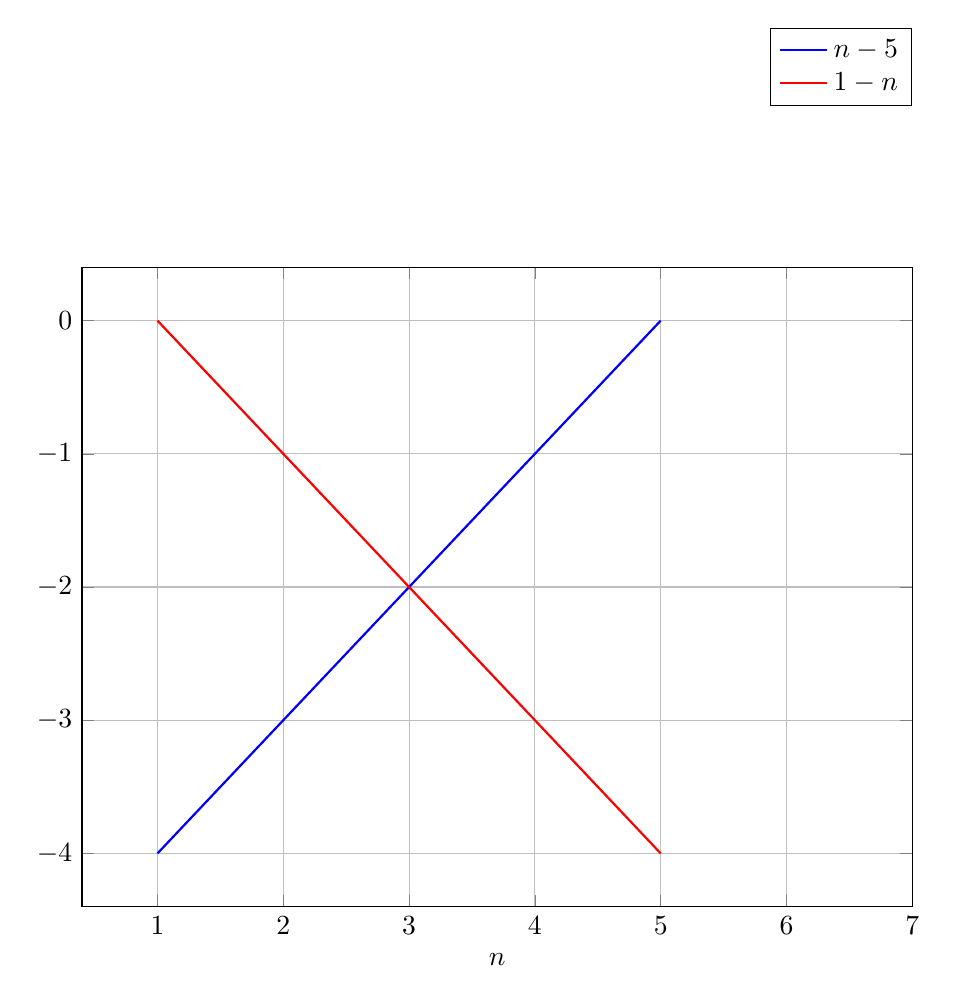
\begin{tikzpicture}
			\begin{axis}[
					xlabel={$n$},
					legend style={at={(axis cs:7,2.2)},anchor=north east},
					grid=major,
					width=\textwidth,
					height=0.8\textwidth,
					xmax=7,
				]
				\addplot[domain=1:5, samples=100, thick, blue] {x-5};
				\addplot[domain=1:5, samples=100, thick, red] {1-x};
				\legend{$n - 5$, $1-n$}
			\end{axis}
		\end{tikzpicture}
		\caption{Negative Distance to Road Boundaries}
		\label{fig:road_boundaries}
	\end{subfigure}
	\hfill
	\begin{subfigure}{0.48\textwidth}
		\centering
		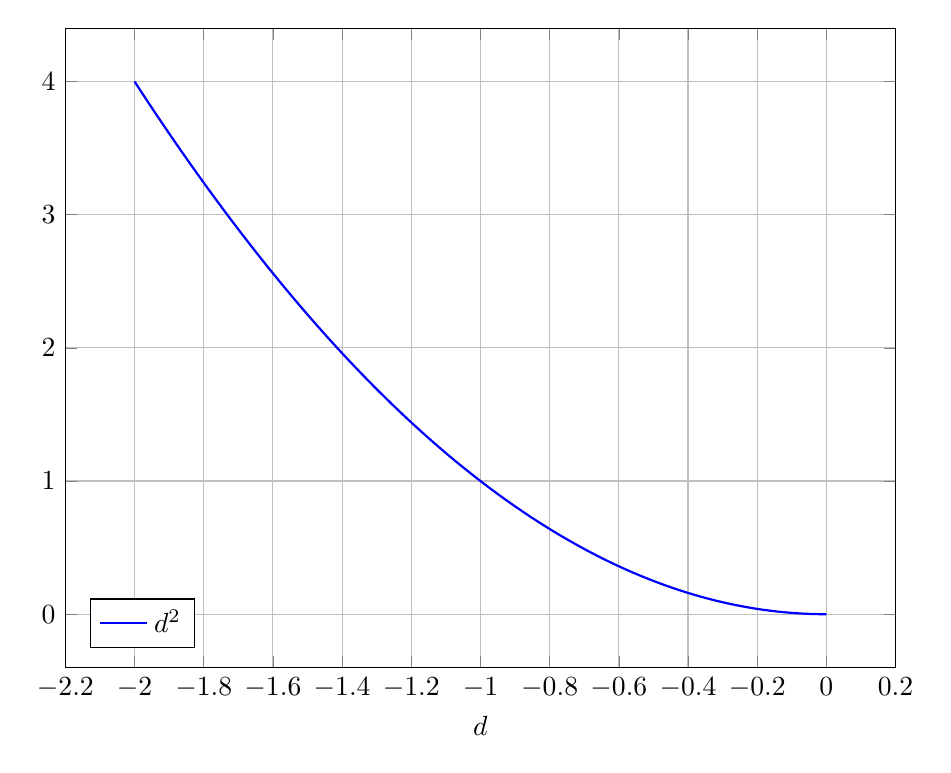
\begin{tikzpicture}
			\begin{axis}[
					xlabel={$d$},
					legend pos=south west,
					grid=major,
					width=\textwidth,
					height=0.8\textwidth
				]
				\addplot[domain=-2:0, samples=100, thick, blue] {x^2};
				\legend{$d^2$}
			\end{axis}
		\end{tikzpicture}
		\caption{Objective Function}
		\label{fig:objective_functions}
	\end{subfigure}
	\caption{Plots the distance to the road boundaries and the objective function.}
	\label{fig:auxiliary_variables}
\end{figure}

While \(\max(x-5, 1-x)\) is a convex function, it is piecewise linear, which can lead to difficulties in optimization.
The benefit of using an auxiliary variable in this context is that it allows us to transform a piecewise linear and potentially non-differentiable
objective function into a smooth and differentiable convex function.
This transformation simplifies the optimization process, making it more efficient and reliable.
Specifically, by introducing the auxiliary variable \( d \) and reformulating the objective as \(\min g(x, u) + d^2\), we obtain a function that is
easier to handle with gradient-based optimization algorithms, which rely on smoothness and differentiability to find optimal solutions effectively.

\subsection{Scenarios} \label{subsec:scenarios}

In order to evaluate the performance of our trajectory planner, we implemented several driving scenarios.
These scenarios are designed to test different aspects of the planner's capabilities.
The Straight Road scenario evaluates the planner's ability to maintain a straight path with minimal control effort, ensuring smooth and efficient
driving.
In the Left Turn scenario, the planner's performance is assessed based on its ability to execute a smooth left turn while adhering to the reference
trajectory.
The Lane Change scenario tests the planner's capability to perform a lane change maneuver safely and efficiently, highlighting its responsiveness and
precision.
The Slalom scenario challenges the planner to navigate through a series of closely spaced obstacles, requiring precise control and smooth transitions
between maneuvers.
The Elchtest, also known as the moose test, evaluates the planner's ability to perform a sudden evasive maneuver to avoid an obstacle, testing its
quick decision-making and control under pressure.
The Elchtest scenario can be visualized as follows:
\begin{figure}[H]
	\centering
	\begin{tikzpicture}
		\draw[thick, dashed] (0,-0.5) -- (5,-0.5); % Road boundary
		\draw[thick, dashed] (0,0.5) -- (3,0.5); % Road boundary
		\draw[thick, dashed] (3,0.5) -- (3,1.5); % Road boundary
		\draw[thick, dashed] (5,0.5) -- (5,-0.5); % Road boundary
		\draw[thick, dashed] (5,0.5) -- (7,0.5); % Road boundary
		\draw[thick, dashed] (3,1.5) -- (9,1.5); % Road boundary
		\draw[thick, dashed] (9,0.5) -- (9,1.5); % Road boundary
		\draw[thick, dashed] (7,0.5) -- (7,-0.5); % Road boundary
		\draw[thick, dashed] (7,-0.5) -- (12,-0.5); % Road boundary
		\draw[thick, dashed] (9,0.5) -- (12,0.5); % Road boundary
		\node at (0,0) {Start};
		\node at (12,0) {End};
	\end{tikzpicture}
	\caption{Elchtest scenario visualization}
	\label{fig:elchtest}
\end{figure}

Finally, the Sharp U Turn scenario tests the planner's ability to execute a sharp U-turn, challenging its control effort and adherence to the desired
terminal state.

By evaluating the planner in these diverse scenarios, we can gain a comprehensive understanding of its strengths and areas for improvement.

\begin{longtable}{l c c c c c}
	\caption{Overview of Road Segments and Their Properties}                                                                                             \\
	\toprule
	\textbf{Road Name}                & \textbf{Segment} & \textbf{Length} & \textbf{Curvature} & \multicolumn{2}{c}{\textbf{Lane Width}}                \\
	\cmidrule(lr){5-6}
	                                  &                  &                 &                    & \textbf{Start}                          & \textbf{End} \\
	\midrule
	\endfirsthead

	\multicolumn{6}{c}{\textit{Continued from previous page}}                                                                                            \\
	\toprule
	\textbf{Road Name}                & \textbf{Segment} & \textbf{Length} & \textbf{Curvature} & \multicolumn{2}{c}{\textbf{Lane Width}}                \\
	\cmidrule(lr){5-6}
	                                  &                  &                 &                    & \textbf{Start}                          & \textbf{End} \\
	\midrule
	\endhead

	\bottomrule
	\multicolumn{6}{c}{\textit{Continued on next page}}                                                                                                  \\
	\endfoot

	\bottomrule
	\endlastfoot

	\multirow{5}{*}{Elchtest}         & 1                & 12.0            & 0.000              & [-1.0,1.0]                              & [-1.0,1.0]   \\
	                                  & 2                & 13.5            & 0.000              & [-1.0,1.0]                              & [2.0,4.7]    \\
	                                  & 3                & 11.0            & 0.000              & [2.0,4.7]                               & [2.0,4.7]    \\
	                                  & 4                & 12.5            & 0.000              & [2.0,4.7]                               & [-1.0,1.0]   \\
	                                  & 5                & 12.0            & 0.000              & [-1.0,1.0]                              & [-1.0,1.0]   \\
	\midrule
	\multirow{1}{*}{Left Turn}        & 1                & 235.6           & 0.007              & [-2.0,2.0]                              & [-2.0,2.0]   \\
	\midrule
	\multirow{1}{*}{Straight}         & 1                & 180.0           & 0.000              & [-2.0,2.0]                              & [-2.0,2.0]   \\
	\midrule
	\multirow{4}{*}{Lane Change}      & 1                & 30.0            & 0.000              & [-2.0,2.0]                              & [-2.0,2.0]   \\
	                                  & 2                & 20.9            & 0.025              & [-2.0,2.0]                              & [-2.0,2.0]   \\
	                                  & 3                & 20.9            & -0.025             & [-2.0,2.0]                              & [-2.0,2.0]   \\
	                                  & 4                & 30.0            & 0.000              & [-2.0,2.0]                              & [-2.0,2.0]   \\
	\midrule
	\multirow{5}{*}{Slalom}           & 1                & 20.0            & 0.000              & [-2.0,2.0]                              & [-2.0,2.0]   \\
	                                  & 2                & 94.2            & -0.033             & [-2.0,2.0]                              & [-2.0,2.0]   \\
	                                  & 3                & 94.2            & 0.033              & [-2.0,2.0]                              & [-2.0,2.0]   \\
	                                  & 4                & 94.2            & -0.033             & [-2.0,2.0]                              & [-2.0,2.0]   \\
	                                  & 5                & 20.0            & 0.000              & [-2.0,2.0]                              & [-2.0,2.0]   \\
	\midrule
	\multirow{3}{*}{Feasible Curve}   & 1                & 20.0            & 0.000              & [-2.0,2.0]                              & [-2.0,2.0]   \\
	                                  & 2                & 15.7            & 0.200              & [-2.0,2.0]                              & [-2.0,2.0]   \\
	                                  & 3                & 20.0            & 0.000              & [-2.0,2.0]                              & [-2.0,2.0]   \\
	\midrule
	\multirow{3}{*}{Infeasible Curve} & 1                & 20.0            & 0.000              & [-2.0,2.0]                              & [-2.0,2.0]   \\
	                                  & 2                & 8.8             & 0.357              & [-2.0,2.0]                              & [-2.0,2.0]   \\
	                                  & 3                & 20.0            & 0.000              & [-2.0,2.0]                              & [-2.0,2.0]   \\
	\midrule
	\label{tab:road_segments}
\end{longtable}

Table \ref{tab:road_segments} provides an overview of the road segments used in our evaluation scenarios.
Each segment is characterized by its length, curvature, and lane width at the start and end points.
This detailed breakdown helps in understanding the specific challenges posed by each scenario and how the trajectory planner adapts to different road
conditions.

\subsection{Simulation Setup} \label{subsec:simulation}

For the vehicle simulation, we employ a more sophisticated model from \cite{noauthor_dateien_2021} and discretize its dynamics using the Runge-Kutta
method \cite{griffiths_rungekutta_2010}, which offers greater accuracy compared to the forward Euler method used for trajectory planning.
To ensure reproducibility, we define the model using the following state variables and control inputs: \[ x = [p_x, p_y, \delta, v, \psi, \dot{\psi},
	\beta]^T, u = [a_x, v_{\delta}]^T \] where $p_x$, $p_y$ represent the vehicle's position coordinates, $\delta$ is the steering angle, $v$ is the
velocity, $\psi$ is the yaw angle, $\dot{\psi}$ is the yaw rate, $\beta$ is the slip angle, $a_x$ is the longitudinal acceleration, and $v_\delta$ is
the steering rate.

The model's dynamics are governed by the following equations, valid for $|v|\geq0.1$:
\[
	f(x, u) = \begin{bmatrix}
		v\cos(\psi + \beta)                                  \\
		v\sin(\psi + \beta)                                  \\
		v_\delta                                             \\
		a_x                                                  \\
		\dot{\psi}                                           \\
		\frac{\mu\,m}{I_{z}(l_{r}+l_{f})}\Bigl(
		l_{f}\,C_{S,f}\bigl(g\,l_{r}-a_xh_{cg}\bigr)\,\delta \\
		\;+                                                 \;\bigl[l_{r}\,C_{S,r}\bigl(g\,l_{f}+a_xh_{cg}\bigr)
			\;-\;l_{f}\,C_{S,f}\bigl(g\,l_{r}-a_xh_{cg}\bigr)\bigr]\,\beta
		\Bigr)                                               \\
		\quad -\;\Bigl[
		l_{f}^{2}\,C_{S,f}\bigl(g\,l_{r}-a_xh_{cg}\bigr)
		\;+\;
		l_{r}^{2}\,C_{S,r}\bigl(g\,l_{f}+a_xh_{cg}\bigr)
		\Bigr]
		\frac{\dot{\psi}}{v}                                 \\
		\frac{\mu}{v\,\bigl(l_{r}+l_{f}\bigr)}\Bigl(
		C_{S,f}\bigl(g\,l_{r}-a_xh_{cg}\bigr)\,\delta
		\;-\;
		\bigl[C_{S,r}\bigl(g\,l_{f}+a_xh_{cg}\bigr)          \\
			\;+\;
		C_{S,f}\bigl(g\,l_{r}-a_xh_{cg}\bigr)\bigr]\,\beta   \\
		\quad +\;\bigl[
			C_{S,r}\bigl(g\,l_{f}+a_xh_{cg}\bigr)\,l_{r}
			\;-\;
			C_{S,f}\bigl(g\,l_{r}-a_xh_{cg}\bigr)\,l_{f}
			\bigr]
		\frac{\dot{\psi}}{v}
		\Bigr)
		\;-\;
		\dot{\psi}
	\end{bmatrix}
\]
For smaller velocities $|v|<0.1$, the dynamics simplify to:
\[
	f(x, u) = \begin{bmatrix}
		v\cos(\psi + \beta) \\
		v\sin(\psi + \beta) \\
		v_\delta            \\
		a_x                 \\
		\dot{\psi}          \\
		\frac{1}{l_{wb}}
		\biggl(
		a_x\,\cos( \beta)\,\tan(\delta)
		\;-\;
		v\,\sin( \beta)\,\tan(\delta)\,\dot{x}_{7}
		\;+\;
		\frac{v\,\cos( \beta)}{\cos^2(\delta)}\,
		v_{\delta}
		\biggr)
		\\
		\frac{1}{1 +
			\bigl(\tan(\delta)\tfrac{l_{r}}{l_{wb}}\bigr)^2}
		\;\cdot\;
		\frac{l_{r}}{l_{wb}\,\cos^2(\delta)}\,
		v_{\delta}
	\end{bmatrix}
\]

We consider a vehicle, with the identifier '1' from \cite{noauthor_dateien_2021} of length \(l = 4.298\,\mathrm{m}\) and width \(w =
1.674\,\mathrm{m}\), with total mass \(m = 1.225\times10^3\,\mathrm{kg}\) and moment of inertia \(I_z = 1.538\times10^3\,\mathrm{kg\,m}^2\).
The center of gravity is located \(l_f = 0.883\,\mathrm{m}\) from the front axle and \(l_r = 1.508\,\mathrm{m}\) from the rear axle, at a height
\(h_{cg} = 0.557\,\mathrm{m}\).
The front and rear cornering stiffness coefficients are both \(C_{S,f} = C_{S,r} = 20.89\,\text{[1/rad]}\), and the friction coefficient is \(\mu =
1.048\).
The switching velocity for the dynamics is set to \(v_S = 4.755\,\mathrm{m/s}\).

\subsection{Results}
\label{subsec:results}

Throughout our simulations, we defined specific ranges for the control inputs to ensure realistic vehicle behavior.
The longitudinal acceleration, $a_x$, was constrained within $[-6, 3]$ m/s², while the steering rate, $v_\delta$, was limited to $[-0.5, 0.5]$ rad/s.
Additionally, the steering angle, $\delta$, was bounded within $[-0.698, 0.698]$ radians.
\[
	a_x \in [-6, 3] \text{ m/s²}, \quad v_\delta \in [-0.5, 0.5] \text{ rad/s}, \quad \delta \in [-0.698, 0.698] \text{ rad}
\]
To evaluate performance under different conditions, we simulated all scenarios at three distinct speeds:
\[
	v_{low}=5 \text{m/s}, v_{mid}=10 \text{m/s}, \text{and } v_{high}=20 \text{m/s}.
\]
We also allowed the vehicle to decelerate down to $70\%$ of its initial speed.

For time discretization, we implemented two configurations, represented as \[ t_{\text{conf}} = (T, R, \Delta t, \Delta^2 t_{\text{replan}}) \] where
$T$ is the time horizon, $R$ is the replanning interval, the initial constant time interval $\Delta t$ for the first few time points, and the
increasing time interval $\Delta^2 t_{\text{replan}}$ for the remaining time points as illustrated in \ref{fig:time_points}.
The first configuration, $t_{\text{conf}}^{(1)}$, was set to a smaller time horizon with a finer $\Delta t$, while the second configuration,
$t_{\text{conf}}^{(2)}$, used a larger time horizon with a coarser $\Delta t$ as well as a smaller slope for the time steps after the replanning
interval, providing two distinct approaches for evaluating planning and control strategies.
\begin{align*}
	t_{\text{conf}}^{(1)} = (3\text{s}, 0.1\text{s}, 10\text{ms}, 40\text{ms}) \\
	t_{\text{conf}}^{(2)} = (5\text{s}, 0.1\text{s}, 20\text{ms}, 20\text{ms})
\end{align*}

We used four objectives to evaluate performance: the control effort cost $J_{control}$, the trajectory tracking cost $J_{tracking}$, the terminal
cost $J_{terminal}$, and the combined cost function $J$ from \eqref{eq:cost_function_combined}, with weighting factors $\alpha = 1$, $\beta = 10^3$,
and $\gamma = 10^4$.
Those weights were chosen to equally balance the objectives.
\[
	J_{control}, J_{tracking}, J_{terminal}, J
\]

All simulations were conducted on a MacBook Air equipped with an Apple M1 processor and 16 GB of unified memory.
The operating system used was macOS 15.3 (24D60).
The simulations were executed using Python 3.11.3, compiled with Clang 13.0.0.

\subsubsection{Solver Times}

This section evaluates solver performance across different models and configurations.
We assessed efficiency by running simulations with varying velocity, scenarios, and objective functions, totaling $96$ simulations per
model-configuration pair.

Table \ref{tab:solver_performance} summarizes the average solver time and its deviation for each model and configuration.

\begin{table}[h]
	\centering
	\caption{Solver Performance for Different Models and Configurations}
	\label{tab:solver_performance}
	\begin{tabular}{lcccc}
		\toprule
		\textbf{Model}    & \textbf{Configuration}  & \textbf{Avg Time (ms)} & \textbf{Time Deviation (ms)} \\
		\midrule
		Double Integrator & $t_{\text{conf}}^{(1)}$ & 3.9                    & 1.0                          \\
		Double Integrator & $t_{\text{conf}}^{(2)}$ & 3.8                    & 1.3                          \\
		Bicycle           & $t_{\text{conf}}^{(1)}$ & 9.5                    & 2.1                          \\
		Bicycle           & $t_{\text{conf}}^{(2)}$ & 9.4                    & 2.9                          \\
		\bottomrule
	\end{tabular}
\end{table}

The double integrator model outperforms the bicycle model, achieving solver times of $3.9$ms and $3.8$ms across both configurations.
In contrast, the bicycle model requires $9.5$ms and $9.4$ms, making it over twice as slow.
Solver time deviations also differ significantly: the double integrator model exhibits deviations of $1.0$ms and $1.3$ms, while the bicycle model
experiences deviations of $2.1$ms and $2.9$ms.

This indicates that the double integrator model provides not only faster solutions but also more stable performance.

\begin{figure}[h!]
	\centering
	\resizebox{\textwidth}{!}{
		\begin{adjustbox}{clip, trim=0cm 0cm 0cm 9.8cm} % left, bottom, right, top
			\input{../code/benchmark-results/slalom-PointMassModel-44e48f14-d19d-4b3f-b484-f84f67a1bcf5/solver_metrics.pgf}
		\end{adjustbox}
	}
	\caption{Solver metrics for Slalom scenario using double integrator model}
	\label{fig:slalom_point_mass_model}
\end{figure}

\begin{figure}[h!]
	\centering
	\resizebox{\textwidth}{!}{
		\begin{adjustbox}{clip, trim=0cm 0cm 0cm 10cm} % left, bottom, right, top
			\input{../code/benchmark-results/slalom-BicycleModel-f33181f3-900a-45bf-88f1-ebadf0bf8a1e/solver_metrics.pgf}
		\end{adjustbox}
	}
	\caption{Solver metrics for Slalom scenario using kinematic bicycle model}
	\label{fig:slalom_bicycle_model}
\end{figure}

Figures \ref{fig:slalom_point_mass_model} and \ref{fig:slalom_bicycle_model} illustrate solver performance in the Slalom scenario.
\begin{itemize}
	\item The double integrator model maintains relatively stable solver times across iterations.
	\item The bicycle model exhibits more variation, aligning with the larger solver time deviations observed in Table \ref{tab:solver_performance}.
\end{itemize}

These findings confirm that the double integrator model provides a more consistent and efficient solution.

\subsubsection{Completion Rates}

Figure \ref{fig:failed_scenarios} presents the number of failed scenarios per model.
As expected, both models fail every test in the Infeasible Curve scenario, which is intentionally designed to be unsolvable.
However, when the curve radius increases slightly (making the scenario marginally feasible), both models successfully complete it at the lowest
velocity $v_{\text{low}}$.

\begin{figure}[h]
	\centering
	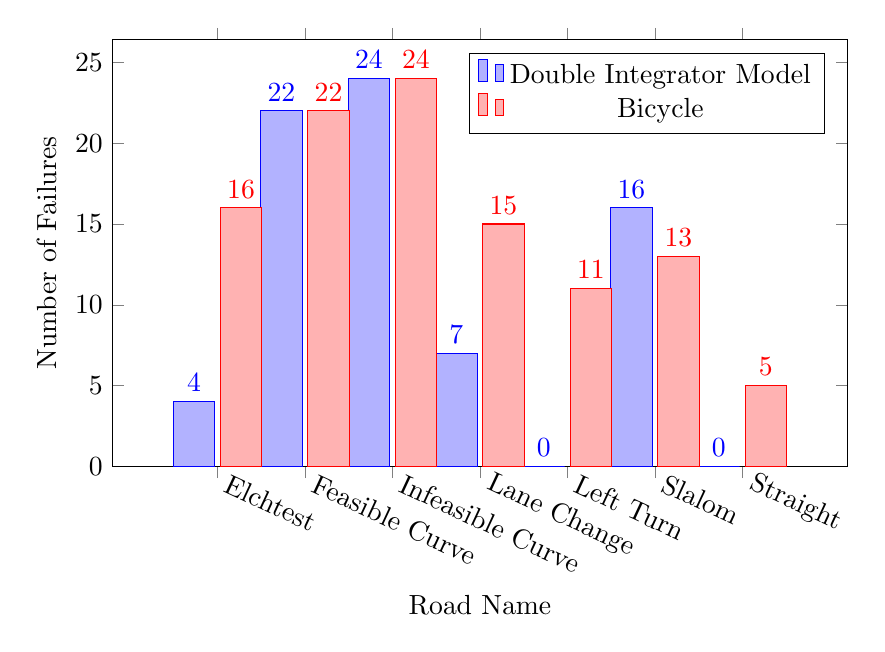
\begin{tikzpicture}
		\begin{axis}[
				ybar,
				bar width=15pt, % Increase bar width
				width=0.9\textwidth, % Increase overall figure width
				height=7cm,
				enlarge x limits=0.2, % Add some space on both sides
				symbolic x coords={Elchtest, Feasible Curve, Infeasible Curve, Lane Change, Left Turn, Slalom, Straight}, % Replace with actual road names
				xtick=data,
				xticklabel style={rotate=-25, anchor=west}, % Rotate labels for readability
				ymin=0,
				ylabel={Number of Failures},
				xlabel={Road Name},
				legend pos=north east,
				nodes near coords
			]
			% Replace the values below with actual failure counts
			\addplot coordinates {(Elchtest,4) (Feasible Curve,22) (Infeasible Curve,24) (Lane Change,7) (Left Turn,0) (Slalom,16) (Straight,0)};
			\addlegendentry{Double Integrator Model}

			\addplot coordinates {(Elchtest,16) (Feasible Curve,22) (Infeasible Curve,24) (Lane Change,15) (Left Turn,11) (Slalom,13) (Straight,5)};
			\addlegendentry{Bicycle}
		\end{axis}
	\end{tikzpicture}
	\caption{Histogram of Failed Scenarios per Model}
	\label{fig:failed_scenarios}
\end{figure}

The results indicate that higher speeds lead to higher failure rates.
However, an anomaly occurs in the Straight scenario, where the bicycle model has a higher failure rate at lower velocities.
This issue arises when using the $J_{\text{terminal}}$ objective function, which prioritizes velocity maximization.
This suggests a numerical instability that may be resolved using soft constraints.

\begin{figure}[h]
	\centering
	\begin{tikzpicture}
		\begin{groupplot}[
				group style={group size=2 by 1, horizontal sep=2cm}, % Two plots side by side
				width=0.5\textwidth, % Adjust width for each plot
				height=7cm,
				symbolic x coords={Elchtest, Feasible Curve, Lane Change, Left Turn, Slalom, Straight}, % Road names
				xtick=data,
				xticklabel style={rotate=-45, anchor=west}, % Rotate labels for readability
				ymin=0,
				ylabel={Number of Failures},
				xlabel={Road Name},
			]

			\nextgroupplot[
				title={Double Integrator Model},
				ybar stacked, % Stacked bars
				bar width=15pt, % Moved inside the groupplot
				nodes near coords, % Show numbers on bars
				every node near coord/.append style={yshift=-1pt}, % Move numbers slightly down
			]
			\addplot coordinates { (Elchtest, 0) (Feasible Curve, 6) (Lane Change, 0) (Left Turn, 0) (Slalom, 8) (Straight, 0) };
			\addplot coordinates { (Elchtest, 0) (Feasible Curve, 8) (Lane Change, 0) (Left Turn, 0) (Slalom, 0) (Straight, 0) };
			\addplot coordinates { (Elchtest, 4) (Feasible Curve, 8) (Lane Change, 7) (Left Turn, 0) (Slalom, 8) (Straight, 0) };
			\legend{5 m/s, 10 m/s, 20 m/s}

			% Second plot: Bicycle Model
			\nextgroupplot[
				title={Kinematic Bicycle Model},
				ybar stacked, % Stacked bars
				bar width=15pt, % Moved inside the groupplot
				nodes near coords, % Show numbers on bars
				every node near coord/.append style={yshift=-1pt}, % Move numbers slightly down
			]
			\addplot coordinates { (Elchtest, 3) (Feasible Curve, 6) (Lane Change, 3) (Left Turn, 2) (Slalom, 3) (Straight, 2) };
			\addplot coordinates { (Elchtest, 5) (Feasible Curve, 8) (Lane Change, 5) (Left Turn, 4) (Slalom, 5) (Straight, 2) };
			\addplot coordinates { (Elchtest, 8) (Feasible Curve, 8) (Lane Change, 7) (Left Turn, 5) (Slalom, 5) (Straight, 1) };
			\legend{5 m/s, 10 m/s, 20 m/s}
		\end{groupplot}
	\end{tikzpicture}
	\caption{Stacked Histogram of Failed Road Names per Model with Velocity}
	\label{fig:failed_scenarios_stacked}
\end{figure}

The bicycle model completes more runs in the slalom scenario compared to the double integrator model.
This is because the double integrator model considers the worst-case scenario and does not find a solution if it is infeasible to drive on the inner
side of the curve, even though it might be feasible to drive on the outer line.
For example driving at the highest speed $v_{max}$, the resulting polytope of the double integrator model is empty.
Limiting the vehicle options to the outer side and reduce the upper speed limit to $14.5$m/s results in a non-empty set.
In fact, we can observe that the bicycle model completes the slalom always at the outer lines (see \ref{fig:slalom_bicycle_model_n}), while driving
at around $14.5$m/s (see \ref{fig:slalom_bicycle_model_velocity}).

\begin{figure}[h!]
	\centering
	\resizebox{\textwidth}{!}{
		\begin{adjustbox}{clip, trim=0cm 14.5cm 0cm 4.8cm}
			%% Creator: Matplotlib, PGF backend
%%
%% To include the figure in your LaTeX document, write
%%   \input{<filename>.pgf}
%%
%% Make sure the required packages are loaded in your preamble
%%   \usepackage{pgf}
%%
%% Also ensure that all the required font packages are loaded; for instance,
%% the lmodern package is sometimes necessary when using math font.
%%   \usepackage{lmodern}
%%
%% Figures using additional raster images can only be included by \input if
%% they are in the same directory as the main LaTeX file. For loading figures
%% from other directories you can use the `import` package
%%   \usepackage{import}
%%
%% and then include the figures with
%%   \import{<path to file>}{<filename>.pgf}
%%
%% Matplotlib used the following preamble
%%   \def\mathdefault#1{#1}
%%   \everymath=\expandafter{\the\everymath\displaystyle}
%%   
%%   \ifdefined\pdftexversion\else  % non-pdftex case.
%%     \usepackage{fontspec}
%%   \fi
%%   \makeatletter\@ifpackageloaded{underscore}{}{\usepackage[strings]{underscore}}\makeatother
%%
\begingroup%
\makeatletter%
\begin{pgfpicture}%
\pgfpathrectangle{\pgfpointorigin}{\pgfqpoint{9.861316in}{9.357149in}}%
\pgfusepath{use as bounding box, clip}%
\begin{pgfscope}%
\pgfsetbuttcap%
\pgfsetmiterjoin%
\definecolor{currentfill}{rgb}{1.000000,1.000000,1.000000}%
\pgfsetfillcolor{currentfill}%
\pgfsetlinewidth{0.000000pt}%
\definecolor{currentstroke}{rgb}{1.000000,1.000000,1.000000}%
\pgfsetstrokecolor{currentstroke}%
\pgfsetdash{}{0pt}%
\pgfpathmoveto{\pgfqpoint{0.000000in}{0.000000in}}%
\pgfpathlineto{\pgfqpoint{9.861316in}{0.000000in}}%
\pgfpathlineto{\pgfqpoint{9.861316in}{9.357149in}}%
\pgfpathlineto{\pgfqpoint{0.000000in}{9.357149in}}%
\pgfpathlineto{\pgfqpoint{0.000000in}{0.000000in}}%
\pgfpathclose%
\pgfusepath{fill}%
\end{pgfscope}%
\begin{pgfscope}%
\pgfsetbuttcap%
\pgfsetmiterjoin%
\definecolor{currentfill}{rgb}{1.000000,1.000000,1.000000}%
\pgfsetfillcolor{currentfill}%
\pgfsetlinewidth{0.000000pt}%
\definecolor{currentstroke}{rgb}{0.000000,0.000000,0.000000}%
\pgfsetstrokecolor{currentstroke}%
\pgfsetstrokeopacity{0.000000}%
\pgfsetdash{}{0pt}%
\pgfpathmoveto{\pgfqpoint{0.716279in}{7.983972in}}%
\pgfpathlineto{\pgfqpoint{9.761316in}{7.983972in}}%
\pgfpathlineto{\pgfqpoint{9.761316in}{9.257149in}}%
\pgfpathlineto{\pgfqpoint{0.716279in}{9.257149in}}%
\pgfpathlineto{\pgfqpoint{0.716279in}{7.983972in}}%
\pgfpathclose%
\pgfusepath{fill}%
\end{pgfscope}%
\begin{pgfscope}%
\pgfsetbuttcap%
\pgfsetroundjoin%
\definecolor{currentfill}{rgb}{0.000000,0.000000,0.000000}%
\pgfsetfillcolor{currentfill}%
\pgfsetlinewidth{0.803000pt}%
\definecolor{currentstroke}{rgb}{0.000000,0.000000,0.000000}%
\pgfsetstrokecolor{currentstroke}%
\pgfsetdash{}{0pt}%
\pgfsys@defobject{currentmarker}{\pgfqpoint{0.000000in}{-0.048611in}}{\pgfqpoint{0.000000in}{0.000000in}}{%
\pgfpathmoveto{\pgfqpoint{0.000000in}{0.000000in}}%
\pgfpathlineto{\pgfqpoint{0.000000in}{-0.048611in}}%
\pgfusepath{stroke,fill}%
}%
\begin{pgfscope}%
\pgfsys@transformshift{1.127417in}{7.983972in}%
\pgfsys@useobject{currentmarker}{}%
\end{pgfscope}%
\end{pgfscope}%
\begin{pgfscope}%
\definecolor{textcolor}{rgb}{0.000000,0.000000,0.000000}%
\pgfsetstrokecolor{textcolor}%
\pgfsetfillcolor{textcolor}%
\pgftext[x=1.127417in,y=7.886750in,,top]{\color{textcolor}{\rmfamily\fontsize{9.000000}{10.800000}\selectfont\catcode`\^=\active\def^{\ifmmode\sp\else\^{}\fi}\catcode`\%=\active\def%{\%}$\mathdefault{0}$}}%
\end{pgfscope}%
\begin{pgfscope}%
\pgfsetbuttcap%
\pgfsetroundjoin%
\definecolor{currentfill}{rgb}{0.000000,0.000000,0.000000}%
\pgfsetfillcolor{currentfill}%
\pgfsetlinewidth{0.803000pt}%
\definecolor{currentstroke}{rgb}{0.000000,0.000000,0.000000}%
\pgfsetstrokecolor{currentstroke}%
\pgfsetdash{}{0pt}%
\pgfsys@defobject{currentmarker}{\pgfqpoint{0.000000in}{-0.048611in}}{\pgfqpoint{0.000000in}{0.000000in}}{%
\pgfpathmoveto{\pgfqpoint{0.000000in}{0.000000in}}%
\pgfpathlineto{\pgfqpoint{0.000000in}{-0.048611in}}%
\pgfusepath{stroke,fill}%
}%
\begin{pgfscope}%
\pgfsys@transformshift{2.402263in}{7.983972in}%
\pgfsys@useobject{currentmarker}{}%
\end{pgfscope}%
\end{pgfscope}%
\begin{pgfscope}%
\definecolor{textcolor}{rgb}{0.000000,0.000000,0.000000}%
\pgfsetstrokecolor{textcolor}%
\pgfsetfillcolor{textcolor}%
\pgftext[x=2.402263in,y=7.886750in,,top]{\color{textcolor}{\rmfamily\fontsize{9.000000}{10.800000}\selectfont\catcode`\^=\active\def^{\ifmmode\sp\else\^{}\fi}\catcode`\%=\active\def%{\%}$\mathdefault{2}$}}%
\end{pgfscope}%
\begin{pgfscope}%
\pgfsetbuttcap%
\pgfsetroundjoin%
\definecolor{currentfill}{rgb}{0.000000,0.000000,0.000000}%
\pgfsetfillcolor{currentfill}%
\pgfsetlinewidth{0.803000pt}%
\definecolor{currentstroke}{rgb}{0.000000,0.000000,0.000000}%
\pgfsetstrokecolor{currentstroke}%
\pgfsetdash{}{0pt}%
\pgfsys@defobject{currentmarker}{\pgfqpoint{0.000000in}{-0.048611in}}{\pgfqpoint{0.000000in}{0.000000in}}{%
\pgfpathmoveto{\pgfqpoint{0.000000in}{0.000000in}}%
\pgfpathlineto{\pgfqpoint{0.000000in}{-0.048611in}}%
\pgfusepath{stroke,fill}%
}%
\begin{pgfscope}%
\pgfsys@transformshift{3.677110in}{7.983972in}%
\pgfsys@useobject{currentmarker}{}%
\end{pgfscope}%
\end{pgfscope}%
\begin{pgfscope}%
\definecolor{textcolor}{rgb}{0.000000,0.000000,0.000000}%
\pgfsetstrokecolor{textcolor}%
\pgfsetfillcolor{textcolor}%
\pgftext[x=3.677110in,y=7.886750in,,top]{\color{textcolor}{\rmfamily\fontsize{9.000000}{10.800000}\selectfont\catcode`\^=\active\def^{\ifmmode\sp\else\^{}\fi}\catcode`\%=\active\def%{\%}$\mathdefault{4}$}}%
\end{pgfscope}%
\begin{pgfscope}%
\pgfsetbuttcap%
\pgfsetroundjoin%
\definecolor{currentfill}{rgb}{0.000000,0.000000,0.000000}%
\pgfsetfillcolor{currentfill}%
\pgfsetlinewidth{0.803000pt}%
\definecolor{currentstroke}{rgb}{0.000000,0.000000,0.000000}%
\pgfsetstrokecolor{currentstroke}%
\pgfsetdash{}{0pt}%
\pgfsys@defobject{currentmarker}{\pgfqpoint{0.000000in}{-0.048611in}}{\pgfqpoint{0.000000in}{0.000000in}}{%
\pgfpathmoveto{\pgfqpoint{0.000000in}{0.000000in}}%
\pgfpathlineto{\pgfqpoint{0.000000in}{-0.048611in}}%
\pgfusepath{stroke,fill}%
}%
\begin{pgfscope}%
\pgfsys@transformshift{4.951957in}{7.983972in}%
\pgfsys@useobject{currentmarker}{}%
\end{pgfscope}%
\end{pgfscope}%
\begin{pgfscope}%
\definecolor{textcolor}{rgb}{0.000000,0.000000,0.000000}%
\pgfsetstrokecolor{textcolor}%
\pgfsetfillcolor{textcolor}%
\pgftext[x=4.951957in,y=7.886750in,,top]{\color{textcolor}{\rmfamily\fontsize{9.000000}{10.800000}\selectfont\catcode`\^=\active\def^{\ifmmode\sp\else\^{}\fi}\catcode`\%=\active\def%{\%}$\mathdefault{6}$}}%
\end{pgfscope}%
\begin{pgfscope}%
\pgfsetbuttcap%
\pgfsetroundjoin%
\definecolor{currentfill}{rgb}{0.000000,0.000000,0.000000}%
\pgfsetfillcolor{currentfill}%
\pgfsetlinewidth{0.803000pt}%
\definecolor{currentstroke}{rgb}{0.000000,0.000000,0.000000}%
\pgfsetstrokecolor{currentstroke}%
\pgfsetdash{}{0pt}%
\pgfsys@defobject{currentmarker}{\pgfqpoint{0.000000in}{-0.048611in}}{\pgfqpoint{0.000000in}{0.000000in}}{%
\pgfpathmoveto{\pgfqpoint{0.000000in}{0.000000in}}%
\pgfpathlineto{\pgfqpoint{0.000000in}{-0.048611in}}%
\pgfusepath{stroke,fill}%
}%
\begin{pgfscope}%
\pgfsys@transformshift{6.226804in}{7.983972in}%
\pgfsys@useobject{currentmarker}{}%
\end{pgfscope}%
\end{pgfscope}%
\begin{pgfscope}%
\definecolor{textcolor}{rgb}{0.000000,0.000000,0.000000}%
\pgfsetstrokecolor{textcolor}%
\pgfsetfillcolor{textcolor}%
\pgftext[x=6.226804in,y=7.886750in,,top]{\color{textcolor}{\rmfamily\fontsize{9.000000}{10.800000}\selectfont\catcode`\^=\active\def^{\ifmmode\sp\else\^{}\fi}\catcode`\%=\active\def%{\%}$\mathdefault{8}$}}%
\end{pgfscope}%
\begin{pgfscope}%
\pgfsetbuttcap%
\pgfsetroundjoin%
\definecolor{currentfill}{rgb}{0.000000,0.000000,0.000000}%
\pgfsetfillcolor{currentfill}%
\pgfsetlinewidth{0.803000pt}%
\definecolor{currentstroke}{rgb}{0.000000,0.000000,0.000000}%
\pgfsetstrokecolor{currentstroke}%
\pgfsetdash{}{0pt}%
\pgfsys@defobject{currentmarker}{\pgfqpoint{0.000000in}{-0.048611in}}{\pgfqpoint{0.000000in}{0.000000in}}{%
\pgfpathmoveto{\pgfqpoint{0.000000in}{0.000000in}}%
\pgfpathlineto{\pgfqpoint{0.000000in}{-0.048611in}}%
\pgfusepath{stroke,fill}%
}%
\begin{pgfscope}%
\pgfsys@transformshift{7.501650in}{7.983972in}%
\pgfsys@useobject{currentmarker}{}%
\end{pgfscope}%
\end{pgfscope}%
\begin{pgfscope}%
\definecolor{textcolor}{rgb}{0.000000,0.000000,0.000000}%
\pgfsetstrokecolor{textcolor}%
\pgfsetfillcolor{textcolor}%
\pgftext[x=7.501650in,y=7.886750in,,top]{\color{textcolor}{\rmfamily\fontsize{9.000000}{10.800000}\selectfont\catcode`\^=\active\def^{\ifmmode\sp\else\^{}\fi}\catcode`\%=\active\def%{\%}$\mathdefault{10}$}}%
\end{pgfscope}%
\begin{pgfscope}%
\pgfsetbuttcap%
\pgfsetroundjoin%
\definecolor{currentfill}{rgb}{0.000000,0.000000,0.000000}%
\pgfsetfillcolor{currentfill}%
\pgfsetlinewidth{0.803000pt}%
\definecolor{currentstroke}{rgb}{0.000000,0.000000,0.000000}%
\pgfsetstrokecolor{currentstroke}%
\pgfsetdash{}{0pt}%
\pgfsys@defobject{currentmarker}{\pgfqpoint{0.000000in}{-0.048611in}}{\pgfqpoint{0.000000in}{0.000000in}}{%
\pgfpathmoveto{\pgfqpoint{0.000000in}{0.000000in}}%
\pgfpathlineto{\pgfqpoint{0.000000in}{-0.048611in}}%
\pgfusepath{stroke,fill}%
}%
\begin{pgfscope}%
\pgfsys@transformshift{8.776497in}{7.983972in}%
\pgfsys@useobject{currentmarker}{}%
\end{pgfscope}%
\end{pgfscope}%
\begin{pgfscope}%
\definecolor{textcolor}{rgb}{0.000000,0.000000,0.000000}%
\pgfsetstrokecolor{textcolor}%
\pgfsetfillcolor{textcolor}%
\pgftext[x=8.776497in,y=7.886750in,,top]{\color{textcolor}{\rmfamily\fontsize{9.000000}{10.800000}\selectfont\catcode`\^=\active\def^{\ifmmode\sp\else\^{}\fi}\catcode`\%=\active\def%{\%}$\mathdefault{12}$}}%
\end{pgfscope}%
\begin{pgfscope}%
\definecolor{textcolor}{rgb}{0.000000,0.000000,0.000000}%
\pgfsetstrokecolor{textcolor}%
\pgfsetfillcolor{textcolor}%
\pgftext[x=5.238797in,y=7.720083in,,top]{\color{textcolor}{\rmfamily\fontsize{11.000000}{13.200000}\selectfont\catcode`\^=\active\def^{\ifmmode\sp\else\^{}\fi}\catcode`\%=\active\def%{\%}Time [s]}}%
\end{pgfscope}%
\begin{pgfscope}%
\pgfsetbuttcap%
\pgfsetroundjoin%
\definecolor{currentfill}{rgb}{0.000000,0.000000,0.000000}%
\pgfsetfillcolor{currentfill}%
\pgfsetlinewidth{0.803000pt}%
\definecolor{currentstroke}{rgb}{0.000000,0.000000,0.000000}%
\pgfsetstrokecolor{currentstroke}%
\pgfsetdash{}{0pt}%
\pgfsys@defobject{currentmarker}{\pgfqpoint{-0.048611in}{0.000000in}}{\pgfqpoint{-0.000000in}{0.000000in}}{%
\pgfpathmoveto{\pgfqpoint{-0.000000in}{0.000000in}}%
\pgfpathlineto{\pgfqpoint{-0.048611in}{0.000000in}}%
\pgfusepath{stroke,fill}%
}%
\begin{pgfscope}%
\pgfsys@transformshift{0.716279in}{8.041844in}%
\pgfsys@useobject{currentmarker}{}%
\end{pgfscope}%
\end{pgfscope}%
\begin{pgfscope}%
\definecolor{textcolor}{rgb}{0.000000,0.000000,0.000000}%
\pgfsetstrokecolor{textcolor}%
\pgfsetfillcolor{textcolor}%
\pgftext[x=0.554821in, y=7.998441in, left, base]{\color{textcolor}{\rmfamily\fontsize{9.000000}{10.800000}\selectfont\catcode`\^=\active\def^{\ifmmode\sp\else\^{}\fi}\catcode`\%=\active\def%{\%}$\mathdefault{0}$}}%
\end{pgfscope}%
\begin{pgfscope}%
\pgfsetbuttcap%
\pgfsetroundjoin%
\definecolor{currentfill}{rgb}{0.000000,0.000000,0.000000}%
\pgfsetfillcolor{currentfill}%
\pgfsetlinewidth{0.803000pt}%
\definecolor{currentstroke}{rgb}{0.000000,0.000000,0.000000}%
\pgfsetstrokecolor{currentstroke}%
\pgfsetdash{}{0pt}%
\pgfsys@defobject{currentmarker}{\pgfqpoint{-0.048611in}{0.000000in}}{\pgfqpoint{-0.000000in}{0.000000in}}{%
\pgfpathmoveto{\pgfqpoint{-0.000000in}{0.000000in}}%
\pgfpathlineto{\pgfqpoint{-0.048611in}{0.000000in}}%
\pgfusepath{stroke,fill}%
}%
\begin{pgfscope}%
\pgfsys@transformshift{0.716279in}{8.318510in}%
\pgfsys@useobject{currentmarker}{}%
\end{pgfscope}%
\end{pgfscope}%
\begin{pgfscope}%
\definecolor{textcolor}{rgb}{0.000000,0.000000,0.000000}%
\pgfsetstrokecolor{textcolor}%
\pgfsetfillcolor{textcolor}%
\pgftext[x=0.490585in, y=8.275107in, left, base]{\color{textcolor}{\rmfamily\fontsize{9.000000}{10.800000}\selectfont\catcode`\^=\active\def^{\ifmmode\sp\else\^{}\fi}\catcode`\%=\active\def%{\%}$\mathdefault{20}$}}%
\end{pgfscope}%
\begin{pgfscope}%
\pgfsetbuttcap%
\pgfsetroundjoin%
\definecolor{currentfill}{rgb}{0.000000,0.000000,0.000000}%
\pgfsetfillcolor{currentfill}%
\pgfsetlinewidth{0.803000pt}%
\definecolor{currentstroke}{rgb}{0.000000,0.000000,0.000000}%
\pgfsetstrokecolor{currentstroke}%
\pgfsetdash{}{0pt}%
\pgfsys@defobject{currentmarker}{\pgfqpoint{-0.048611in}{0.000000in}}{\pgfqpoint{-0.000000in}{0.000000in}}{%
\pgfpathmoveto{\pgfqpoint{-0.000000in}{0.000000in}}%
\pgfpathlineto{\pgfqpoint{-0.048611in}{0.000000in}}%
\pgfusepath{stroke,fill}%
}%
\begin{pgfscope}%
\pgfsys@transformshift{0.716279in}{8.595176in}%
\pgfsys@useobject{currentmarker}{}%
\end{pgfscope}%
\end{pgfscope}%
\begin{pgfscope}%
\definecolor{textcolor}{rgb}{0.000000,0.000000,0.000000}%
\pgfsetstrokecolor{textcolor}%
\pgfsetfillcolor{textcolor}%
\pgftext[x=0.490585in, y=8.551773in, left, base]{\color{textcolor}{\rmfamily\fontsize{9.000000}{10.800000}\selectfont\catcode`\^=\active\def^{\ifmmode\sp\else\^{}\fi}\catcode`\%=\active\def%{\%}$\mathdefault{40}$}}%
\end{pgfscope}%
\begin{pgfscope}%
\pgfsetbuttcap%
\pgfsetroundjoin%
\definecolor{currentfill}{rgb}{0.000000,0.000000,0.000000}%
\pgfsetfillcolor{currentfill}%
\pgfsetlinewidth{0.803000pt}%
\definecolor{currentstroke}{rgb}{0.000000,0.000000,0.000000}%
\pgfsetstrokecolor{currentstroke}%
\pgfsetdash{}{0pt}%
\pgfsys@defobject{currentmarker}{\pgfqpoint{-0.048611in}{0.000000in}}{\pgfqpoint{-0.000000in}{0.000000in}}{%
\pgfpathmoveto{\pgfqpoint{-0.000000in}{0.000000in}}%
\pgfpathlineto{\pgfqpoint{-0.048611in}{0.000000in}}%
\pgfusepath{stroke,fill}%
}%
\begin{pgfscope}%
\pgfsys@transformshift{0.716279in}{8.871842in}%
\pgfsys@useobject{currentmarker}{}%
\end{pgfscope}%
\end{pgfscope}%
\begin{pgfscope}%
\definecolor{textcolor}{rgb}{0.000000,0.000000,0.000000}%
\pgfsetstrokecolor{textcolor}%
\pgfsetfillcolor{textcolor}%
\pgftext[x=0.490585in, y=8.828439in, left, base]{\color{textcolor}{\rmfamily\fontsize{9.000000}{10.800000}\selectfont\catcode`\^=\active\def^{\ifmmode\sp\else\^{}\fi}\catcode`\%=\active\def%{\%}$\mathdefault{60}$}}%
\end{pgfscope}%
\begin{pgfscope}%
\pgfsetbuttcap%
\pgfsetroundjoin%
\definecolor{currentfill}{rgb}{0.000000,0.000000,0.000000}%
\pgfsetfillcolor{currentfill}%
\pgfsetlinewidth{0.803000pt}%
\definecolor{currentstroke}{rgb}{0.000000,0.000000,0.000000}%
\pgfsetstrokecolor{currentstroke}%
\pgfsetdash{}{0pt}%
\pgfsys@defobject{currentmarker}{\pgfqpoint{-0.048611in}{0.000000in}}{\pgfqpoint{-0.000000in}{0.000000in}}{%
\pgfpathmoveto{\pgfqpoint{-0.000000in}{0.000000in}}%
\pgfpathlineto{\pgfqpoint{-0.048611in}{0.000000in}}%
\pgfusepath{stroke,fill}%
}%
\begin{pgfscope}%
\pgfsys@transformshift{0.716279in}{9.148508in}%
\pgfsys@useobject{currentmarker}{}%
\end{pgfscope}%
\end{pgfscope}%
\begin{pgfscope}%
\definecolor{textcolor}{rgb}{0.000000,0.000000,0.000000}%
\pgfsetstrokecolor{textcolor}%
\pgfsetfillcolor{textcolor}%
\pgftext[x=0.490585in, y=9.105105in, left, base]{\color{textcolor}{\rmfamily\fontsize{9.000000}{10.800000}\selectfont\catcode`\^=\active\def^{\ifmmode\sp\else\^{}\fi}\catcode`\%=\active\def%{\%}$\mathdefault{80}$}}%
\end{pgfscope}%
\begin{pgfscope}%
\definecolor{textcolor}{rgb}{0.000000,0.000000,0.000000}%
\pgfsetstrokecolor{textcolor}%
\pgfsetfillcolor{textcolor}%
\pgftext[x=0.435029in,y=8.620561in,,bottom,rotate=90.000000]{\color{textcolor}{\rmfamily\fontsize{11.000000}{13.200000}\selectfont\catcode`\^=\active\def^{\ifmmode\sp\else\^{}\fi}\catcode`\%=\active\def%{\%}s}}%
\end{pgfscope}%
\begin{pgfscope}%
\pgfpathrectangle{\pgfqpoint{0.716279in}{7.983972in}}{\pgfqpoint{9.045038in}{1.273177in}}%
\pgfusepath{clip}%
\pgfsetrectcap%
\pgfsetroundjoin%
\pgfsetlinewidth{1.505625pt}%
\definecolor{currentstroke}{rgb}{0.000000,0.000000,1.000000}%
\pgfsetstrokecolor{currentstroke}%
\pgfsetdash{}{0pt}%
\pgfpathmoveto{\pgfqpoint{1.140165in}{8.043227in}}%
\pgfpathlineto{\pgfqpoint{1.280398in}{8.059641in}}%
\pgfpathlineto{\pgfqpoint{1.420631in}{8.078063in}}%
\pgfpathlineto{\pgfqpoint{1.803085in}{8.132063in}}%
\pgfpathlineto{\pgfqpoint{2.096300in}{8.173375in}}%
\pgfpathlineto{\pgfqpoint{2.963196in}{8.295757in}}%
\pgfpathlineto{\pgfqpoint{3.116178in}{8.317241in}}%
\pgfpathlineto{\pgfqpoint{3.983073in}{8.439621in}}%
\pgfpathlineto{\pgfqpoint{4.136055in}{8.461097in}}%
\pgfpathlineto{\pgfqpoint{5.908092in}{8.712256in}}%
\pgfpathlineto{\pgfqpoint{8.049834in}{9.015474in}}%
\pgfpathlineto{\pgfqpoint{8.381295in}{9.062387in}}%
\pgfpathlineto{\pgfqpoint{8.534276in}{9.083864in}}%
\pgfpathlineto{\pgfqpoint{9.350178in}{9.199277in}}%
\pgfpathlineto{\pgfqpoint{9.350178in}{9.199277in}}%
\pgfusepath{stroke}%
\end{pgfscope}%
\begin{pgfscope}%
\pgfpathrectangle{\pgfqpoint{0.716279in}{7.983972in}}{\pgfqpoint{9.045038in}{1.273177in}}%
\pgfusepath{clip}%
\pgfsetrectcap%
\pgfsetroundjoin%
\pgfsetlinewidth{1.505625pt}%
\definecolor{currentstroke}{rgb}{1.000000,0.000000,0.000000}%
\pgfsetstrokecolor{currentstroke}%
\pgfsetdash{}{0pt}%
\pgfpathmoveto{\pgfqpoint{0.000000in}{0.000000in}}%
\pgfusepath{stroke}%
\end{pgfscope}%
\begin{pgfscope}%
\pgfpathrectangle{\pgfqpoint{0.716279in}{7.983972in}}{\pgfqpoint{9.045038in}{1.273177in}}%
\pgfusepath{clip}%
\pgfsetrectcap%
\pgfsetroundjoin%
\pgfsetlinewidth{1.505625pt}%
\definecolor{currentstroke}{rgb}{0.000000,0.501961,0.000000}%
\pgfsetstrokecolor{currentstroke}%
\pgfsetdash{}{0pt}%
\pgfpathmoveto{\pgfqpoint{1.127417in}{8.041844in}}%
\pgfusepath{stroke}%
\end{pgfscope}%
\begin{pgfscope}%
\pgfsetrectcap%
\pgfsetmiterjoin%
\pgfsetlinewidth{0.803000pt}%
\definecolor{currentstroke}{rgb}{0.000000,0.000000,0.000000}%
\pgfsetstrokecolor{currentstroke}%
\pgfsetdash{}{0pt}%
\pgfpathmoveto{\pgfqpoint{0.716279in}{7.983972in}}%
\pgfpathlineto{\pgfqpoint{0.716279in}{9.257149in}}%
\pgfusepath{stroke}%
\end{pgfscope}%
\begin{pgfscope}%
\pgfsetrectcap%
\pgfsetmiterjoin%
\pgfsetlinewidth{0.803000pt}%
\definecolor{currentstroke}{rgb}{0.000000,0.000000,0.000000}%
\pgfsetstrokecolor{currentstroke}%
\pgfsetdash{}{0pt}%
\pgfpathmoveto{\pgfqpoint{9.761316in}{7.983972in}}%
\pgfpathlineto{\pgfqpoint{9.761316in}{9.257149in}}%
\pgfusepath{stroke}%
\end{pgfscope}%
\begin{pgfscope}%
\pgfsetrectcap%
\pgfsetmiterjoin%
\pgfsetlinewidth{0.803000pt}%
\definecolor{currentstroke}{rgb}{0.000000,0.000000,0.000000}%
\pgfsetstrokecolor{currentstroke}%
\pgfsetdash{}{0pt}%
\pgfpathmoveto{\pgfqpoint{0.716279in}{7.983972in}}%
\pgfpathlineto{\pgfqpoint{9.761316in}{7.983972in}}%
\pgfusepath{stroke}%
\end{pgfscope}%
\begin{pgfscope}%
\pgfsetrectcap%
\pgfsetmiterjoin%
\pgfsetlinewidth{0.803000pt}%
\definecolor{currentstroke}{rgb}{0.000000,0.000000,0.000000}%
\pgfsetstrokecolor{currentstroke}%
\pgfsetdash{}{0pt}%
\pgfpathmoveto{\pgfqpoint{0.716279in}{9.257149in}}%
\pgfpathlineto{\pgfqpoint{9.761316in}{9.257149in}}%
\pgfusepath{stroke}%
\end{pgfscope}%
\begin{pgfscope}%
\pgfsetbuttcap%
\pgfsetmiterjoin%
\definecolor{currentfill}{rgb}{1.000000,1.000000,1.000000}%
\pgfsetfillcolor{currentfill}%
\pgfsetfillopacity{0.800000}%
\pgfsetlinewidth{1.003750pt}%
\definecolor{currentstroke}{rgb}{0.800000,0.800000,0.800000}%
\pgfsetstrokecolor{currentstroke}%
\pgfsetstrokeopacity{0.800000}%
\pgfsetdash{}{0pt}%
\pgfpathmoveto{\pgfqpoint{0.813501in}{8.565019in}}%
\pgfpathlineto{\pgfqpoint{1.481711in}{8.565019in}}%
\pgfpathquadraticcurveto{\pgfqpoint{1.509489in}{8.565019in}}{\pgfqpoint{1.509489in}{8.592797in}}%
\pgfpathlineto{\pgfqpoint{1.509489in}{9.159927in}}%
\pgfpathquadraticcurveto{\pgfqpoint{1.509489in}{9.187704in}}{\pgfqpoint{1.481711in}{9.187704in}}%
\pgfpathlineto{\pgfqpoint{0.813501in}{9.187704in}}%
\pgfpathquadraticcurveto{\pgfqpoint{0.785723in}{9.187704in}}{\pgfqpoint{0.785723in}{9.159927in}}%
\pgfpathlineto{\pgfqpoint{0.785723in}{8.592797in}}%
\pgfpathquadraticcurveto{\pgfqpoint{0.785723in}{8.565019in}}{\pgfqpoint{0.813501in}{8.565019in}}%
\pgfpathlineto{\pgfqpoint{0.813501in}{8.565019in}}%
\pgfpathclose%
\pgfusepath{stroke,fill}%
\end{pgfscope}%
\begin{pgfscope}%
\pgfsetrectcap%
\pgfsetroundjoin%
\pgfsetlinewidth{1.505625pt}%
\definecolor{currentstroke}{rgb}{0.000000,0.000000,1.000000}%
\pgfsetstrokecolor{currentstroke}%
\pgfsetdash{}{0pt}%
\pgfpathmoveto{\pgfqpoint{0.841279in}{9.083538in}}%
\pgfpathlineto{\pgfqpoint{0.980168in}{9.083538in}}%
\pgfpathlineto{\pgfqpoint{1.119056in}{9.083538in}}%
\pgfusepath{stroke}%
\end{pgfscope}%
\begin{pgfscope}%
\definecolor{textcolor}{rgb}{0.000000,0.000000,0.000000}%
\pgfsetstrokecolor{textcolor}%
\pgfsetfillcolor{textcolor}%
\pgftext[x=1.230168in,y=9.034927in,left,base]{\color{textcolor}{\rmfamily\fontsize{10.000000}{12.000000}\selectfont\catcode`\^=\active\def^{\ifmmode\sp\else\^{}\fi}\catcode`\%=\active\def%{\%}pos}}%
\end{pgfscope}%
\begin{pgfscope}%
\pgfsetrectcap%
\pgfsetroundjoin%
\pgfsetlinewidth{1.505625pt}%
\definecolor{currentstroke}{rgb}{1.000000,0.000000,0.000000}%
\pgfsetstrokecolor{currentstroke}%
\pgfsetdash{}{0pt}%
\pgfpathmoveto{\pgfqpoint{0.841279in}{8.889865in}}%
\pgfpathlineto{\pgfqpoint{0.980168in}{8.889865in}}%
\pgfpathlineto{\pgfqpoint{1.119056in}{8.889865in}}%
\pgfusepath{stroke}%
\end{pgfscope}%
\begin{pgfscope}%
\definecolor{textcolor}{rgb}{0.000000,0.000000,0.000000}%
\pgfsetstrokecolor{textcolor}%
\pgfsetfillcolor{textcolor}%
\pgftext[x=1.230168in,y=8.841254in,left,base]{\color{textcolor}{\rmfamily\fontsize{10.000000}{12.000000}\selectfont\catcode`\^=\active\def^{\ifmmode\sp\else\^{}\fi}\catcode`\%=\active\def%{\%}neg}}%
\end{pgfscope}%
\begin{pgfscope}%
\pgfsetrectcap%
\pgfsetroundjoin%
\pgfsetlinewidth{1.505625pt}%
\definecolor{currentstroke}{rgb}{0.000000,0.501961,0.000000}%
\pgfsetstrokecolor{currentstroke}%
\pgfsetdash{}{0pt}%
\pgfpathmoveto{\pgfqpoint{0.841279in}{8.696192in}}%
\pgfpathlineto{\pgfqpoint{0.980168in}{8.696192in}}%
\pgfpathlineto{\pgfqpoint{1.119056in}{8.696192in}}%
\pgfusepath{stroke}%
\end{pgfscope}%
\begin{pgfscope}%
\definecolor{textcolor}{rgb}{0.000000,0.000000,0.000000}%
\pgfsetstrokecolor{textcolor}%
\pgfsetfillcolor{textcolor}%
\pgftext[x=1.230168in,y=8.647581in,left,base]{\color{textcolor}{\rmfamily\fontsize{10.000000}{12.000000}\selectfont\catcode`\^=\active\def^{\ifmmode\sp\else\^{}\fi}\catcode`\%=\active\def%{\%}= 0}}%
\end{pgfscope}%
\begin{pgfscope}%
\pgfsetbuttcap%
\pgfsetmiterjoin%
\definecolor{currentfill}{rgb}{1.000000,1.000000,1.000000}%
\pgfsetfillcolor{currentfill}%
\pgfsetlinewidth{0.000000pt}%
\definecolor{currentstroke}{rgb}{0.000000,0.000000,0.000000}%
\pgfsetstrokecolor{currentstroke}%
\pgfsetstrokeopacity{0.000000}%
\pgfsetdash{}{0pt}%
\pgfpathmoveto{\pgfqpoint{0.716279in}{6.116972in}}%
\pgfpathlineto{\pgfqpoint{9.761316in}{6.116972in}}%
\pgfpathlineto{\pgfqpoint{9.761316in}{7.390149in}}%
\pgfpathlineto{\pgfqpoint{0.716279in}{7.390149in}}%
\pgfpathlineto{\pgfqpoint{0.716279in}{6.116972in}}%
\pgfpathclose%
\pgfusepath{fill}%
\end{pgfscope}%
\begin{pgfscope}%
\pgfsetbuttcap%
\pgfsetroundjoin%
\definecolor{currentfill}{rgb}{0.000000,0.000000,0.000000}%
\pgfsetfillcolor{currentfill}%
\pgfsetlinewidth{0.803000pt}%
\definecolor{currentstroke}{rgb}{0.000000,0.000000,0.000000}%
\pgfsetstrokecolor{currentstroke}%
\pgfsetdash{}{0pt}%
\pgfsys@defobject{currentmarker}{\pgfqpoint{0.000000in}{-0.048611in}}{\pgfqpoint{0.000000in}{0.000000in}}{%
\pgfpathmoveto{\pgfqpoint{0.000000in}{0.000000in}}%
\pgfpathlineto{\pgfqpoint{0.000000in}{-0.048611in}}%
\pgfusepath{stroke,fill}%
}%
\begin{pgfscope}%
\pgfsys@transformshift{1.127417in}{6.116972in}%
\pgfsys@useobject{currentmarker}{}%
\end{pgfscope}%
\end{pgfscope}%
\begin{pgfscope}%
\definecolor{textcolor}{rgb}{0.000000,0.000000,0.000000}%
\pgfsetstrokecolor{textcolor}%
\pgfsetfillcolor{textcolor}%
\pgftext[x=1.127417in,y=6.019750in,,top]{\color{textcolor}{\rmfamily\fontsize{9.000000}{10.800000}\selectfont\catcode`\^=\active\def^{\ifmmode\sp\else\^{}\fi}\catcode`\%=\active\def%{\%}$\mathdefault{0}$}}%
\end{pgfscope}%
\begin{pgfscope}%
\pgfsetbuttcap%
\pgfsetroundjoin%
\definecolor{currentfill}{rgb}{0.000000,0.000000,0.000000}%
\pgfsetfillcolor{currentfill}%
\pgfsetlinewidth{0.803000pt}%
\definecolor{currentstroke}{rgb}{0.000000,0.000000,0.000000}%
\pgfsetstrokecolor{currentstroke}%
\pgfsetdash{}{0pt}%
\pgfsys@defobject{currentmarker}{\pgfqpoint{0.000000in}{-0.048611in}}{\pgfqpoint{0.000000in}{0.000000in}}{%
\pgfpathmoveto{\pgfqpoint{0.000000in}{0.000000in}}%
\pgfpathlineto{\pgfqpoint{0.000000in}{-0.048611in}}%
\pgfusepath{stroke,fill}%
}%
\begin{pgfscope}%
\pgfsys@transformshift{2.402263in}{6.116972in}%
\pgfsys@useobject{currentmarker}{}%
\end{pgfscope}%
\end{pgfscope}%
\begin{pgfscope}%
\definecolor{textcolor}{rgb}{0.000000,0.000000,0.000000}%
\pgfsetstrokecolor{textcolor}%
\pgfsetfillcolor{textcolor}%
\pgftext[x=2.402263in,y=6.019750in,,top]{\color{textcolor}{\rmfamily\fontsize{9.000000}{10.800000}\selectfont\catcode`\^=\active\def^{\ifmmode\sp\else\^{}\fi}\catcode`\%=\active\def%{\%}$\mathdefault{2}$}}%
\end{pgfscope}%
\begin{pgfscope}%
\pgfsetbuttcap%
\pgfsetroundjoin%
\definecolor{currentfill}{rgb}{0.000000,0.000000,0.000000}%
\pgfsetfillcolor{currentfill}%
\pgfsetlinewidth{0.803000pt}%
\definecolor{currentstroke}{rgb}{0.000000,0.000000,0.000000}%
\pgfsetstrokecolor{currentstroke}%
\pgfsetdash{}{0pt}%
\pgfsys@defobject{currentmarker}{\pgfqpoint{0.000000in}{-0.048611in}}{\pgfqpoint{0.000000in}{0.000000in}}{%
\pgfpathmoveto{\pgfqpoint{0.000000in}{0.000000in}}%
\pgfpathlineto{\pgfqpoint{0.000000in}{-0.048611in}}%
\pgfusepath{stroke,fill}%
}%
\begin{pgfscope}%
\pgfsys@transformshift{3.677110in}{6.116972in}%
\pgfsys@useobject{currentmarker}{}%
\end{pgfscope}%
\end{pgfscope}%
\begin{pgfscope}%
\definecolor{textcolor}{rgb}{0.000000,0.000000,0.000000}%
\pgfsetstrokecolor{textcolor}%
\pgfsetfillcolor{textcolor}%
\pgftext[x=3.677110in,y=6.019750in,,top]{\color{textcolor}{\rmfamily\fontsize{9.000000}{10.800000}\selectfont\catcode`\^=\active\def^{\ifmmode\sp\else\^{}\fi}\catcode`\%=\active\def%{\%}$\mathdefault{4}$}}%
\end{pgfscope}%
\begin{pgfscope}%
\pgfsetbuttcap%
\pgfsetroundjoin%
\definecolor{currentfill}{rgb}{0.000000,0.000000,0.000000}%
\pgfsetfillcolor{currentfill}%
\pgfsetlinewidth{0.803000pt}%
\definecolor{currentstroke}{rgb}{0.000000,0.000000,0.000000}%
\pgfsetstrokecolor{currentstroke}%
\pgfsetdash{}{0pt}%
\pgfsys@defobject{currentmarker}{\pgfqpoint{0.000000in}{-0.048611in}}{\pgfqpoint{0.000000in}{0.000000in}}{%
\pgfpathmoveto{\pgfqpoint{0.000000in}{0.000000in}}%
\pgfpathlineto{\pgfqpoint{0.000000in}{-0.048611in}}%
\pgfusepath{stroke,fill}%
}%
\begin{pgfscope}%
\pgfsys@transformshift{4.951957in}{6.116972in}%
\pgfsys@useobject{currentmarker}{}%
\end{pgfscope}%
\end{pgfscope}%
\begin{pgfscope}%
\definecolor{textcolor}{rgb}{0.000000,0.000000,0.000000}%
\pgfsetstrokecolor{textcolor}%
\pgfsetfillcolor{textcolor}%
\pgftext[x=4.951957in,y=6.019750in,,top]{\color{textcolor}{\rmfamily\fontsize{9.000000}{10.800000}\selectfont\catcode`\^=\active\def^{\ifmmode\sp\else\^{}\fi}\catcode`\%=\active\def%{\%}$\mathdefault{6}$}}%
\end{pgfscope}%
\begin{pgfscope}%
\pgfsetbuttcap%
\pgfsetroundjoin%
\definecolor{currentfill}{rgb}{0.000000,0.000000,0.000000}%
\pgfsetfillcolor{currentfill}%
\pgfsetlinewidth{0.803000pt}%
\definecolor{currentstroke}{rgb}{0.000000,0.000000,0.000000}%
\pgfsetstrokecolor{currentstroke}%
\pgfsetdash{}{0pt}%
\pgfsys@defobject{currentmarker}{\pgfqpoint{0.000000in}{-0.048611in}}{\pgfqpoint{0.000000in}{0.000000in}}{%
\pgfpathmoveto{\pgfqpoint{0.000000in}{0.000000in}}%
\pgfpathlineto{\pgfqpoint{0.000000in}{-0.048611in}}%
\pgfusepath{stroke,fill}%
}%
\begin{pgfscope}%
\pgfsys@transformshift{6.226804in}{6.116972in}%
\pgfsys@useobject{currentmarker}{}%
\end{pgfscope}%
\end{pgfscope}%
\begin{pgfscope}%
\definecolor{textcolor}{rgb}{0.000000,0.000000,0.000000}%
\pgfsetstrokecolor{textcolor}%
\pgfsetfillcolor{textcolor}%
\pgftext[x=6.226804in,y=6.019750in,,top]{\color{textcolor}{\rmfamily\fontsize{9.000000}{10.800000}\selectfont\catcode`\^=\active\def^{\ifmmode\sp\else\^{}\fi}\catcode`\%=\active\def%{\%}$\mathdefault{8}$}}%
\end{pgfscope}%
\begin{pgfscope}%
\pgfsetbuttcap%
\pgfsetroundjoin%
\definecolor{currentfill}{rgb}{0.000000,0.000000,0.000000}%
\pgfsetfillcolor{currentfill}%
\pgfsetlinewidth{0.803000pt}%
\definecolor{currentstroke}{rgb}{0.000000,0.000000,0.000000}%
\pgfsetstrokecolor{currentstroke}%
\pgfsetdash{}{0pt}%
\pgfsys@defobject{currentmarker}{\pgfqpoint{0.000000in}{-0.048611in}}{\pgfqpoint{0.000000in}{0.000000in}}{%
\pgfpathmoveto{\pgfqpoint{0.000000in}{0.000000in}}%
\pgfpathlineto{\pgfqpoint{0.000000in}{-0.048611in}}%
\pgfusepath{stroke,fill}%
}%
\begin{pgfscope}%
\pgfsys@transformshift{7.501650in}{6.116972in}%
\pgfsys@useobject{currentmarker}{}%
\end{pgfscope}%
\end{pgfscope}%
\begin{pgfscope}%
\definecolor{textcolor}{rgb}{0.000000,0.000000,0.000000}%
\pgfsetstrokecolor{textcolor}%
\pgfsetfillcolor{textcolor}%
\pgftext[x=7.501650in,y=6.019750in,,top]{\color{textcolor}{\rmfamily\fontsize{9.000000}{10.800000}\selectfont\catcode`\^=\active\def^{\ifmmode\sp\else\^{}\fi}\catcode`\%=\active\def%{\%}$\mathdefault{10}$}}%
\end{pgfscope}%
\begin{pgfscope}%
\pgfsetbuttcap%
\pgfsetroundjoin%
\definecolor{currentfill}{rgb}{0.000000,0.000000,0.000000}%
\pgfsetfillcolor{currentfill}%
\pgfsetlinewidth{0.803000pt}%
\definecolor{currentstroke}{rgb}{0.000000,0.000000,0.000000}%
\pgfsetstrokecolor{currentstroke}%
\pgfsetdash{}{0pt}%
\pgfsys@defobject{currentmarker}{\pgfqpoint{0.000000in}{-0.048611in}}{\pgfqpoint{0.000000in}{0.000000in}}{%
\pgfpathmoveto{\pgfqpoint{0.000000in}{0.000000in}}%
\pgfpathlineto{\pgfqpoint{0.000000in}{-0.048611in}}%
\pgfusepath{stroke,fill}%
}%
\begin{pgfscope}%
\pgfsys@transformshift{8.776497in}{6.116972in}%
\pgfsys@useobject{currentmarker}{}%
\end{pgfscope}%
\end{pgfscope}%
\begin{pgfscope}%
\definecolor{textcolor}{rgb}{0.000000,0.000000,0.000000}%
\pgfsetstrokecolor{textcolor}%
\pgfsetfillcolor{textcolor}%
\pgftext[x=8.776497in,y=6.019750in,,top]{\color{textcolor}{\rmfamily\fontsize{9.000000}{10.800000}\selectfont\catcode`\^=\active\def^{\ifmmode\sp\else\^{}\fi}\catcode`\%=\active\def%{\%}$\mathdefault{12}$}}%
\end{pgfscope}%
\begin{pgfscope}%
\definecolor{textcolor}{rgb}{0.000000,0.000000,0.000000}%
\pgfsetstrokecolor{textcolor}%
\pgfsetfillcolor{textcolor}%
\pgftext[x=5.238797in,y=5.853083in,,top]{\color{textcolor}{\rmfamily\fontsize{11.000000}{13.200000}\selectfont\catcode`\^=\active\def^{\ifmmode\sp\else\^{}\fi}\catcode`\%=\active\def%{\%}Time [s]}}%
\end{pgfscope}%
\begin{pgfscope}%
\pgfsetbuttcap%
\pgfsetroundjoin%
\definecolor{currentfill}{rgb}{0.000000,0.000000,0.000000}%
\pgfsetfillcolor{currentfill}%
\pgfsetlinewidth{0.803000pt}%
\definecolor{currentstroke}{rgb}{0.000000,0.000000,0.000000}%
\pgfsetstrokecolor{currentstroke}%
\pgfsetdash{}{0pt}%
\pgfsys@defobject{currentmarker}{\pgfqpoint{-0.048611in}{0.000000in}}{\pgfqpoint{-0.000000in}{0.000000in}}{%
\pgfpathmoveto{\pgfqpoint{-0.000000in}{0.000000in}}%
\pgfpathlineto{\pgfqpoint{-0.048611in}{0.000000in}}%
\pgfusepath{stroke,fill}%
}%
\begin{pgfscope}%
\pgfsys@transformshift{0.716279in}{6.309572in}%
\pgfsys@useobject{currentmarker}{}%
\end{pgfscope}%
\end{pgfscope}%
\begin{pgfscope}%
\definecolor{textcolor}{rgb}{0.000000,0.000000,0.000000}%
\pgfsetstrokecolor{textcolor}%
\pgfsetfillcolor{textcolor}%
\pgftext[x=0.354976in, y=6.266169in, left, base]{\color{textcolor}{\rmfamily\fontsize{9.000000}{10.800000}\selectfont\catcode`\^=\active\def^{\ifmmode\sp\else\^{}\fi}\catcode`\%=\active\def%{\%}$\mathdefault{\ensuremath{-}0.2}$}}%
\end{pgfscope}%
\begin{pgfscope}%
\pgfsetbuttcap%
\pgfsetroundjoin%
\definecolor{currentfill}{rgb}{0.000000,0.000000,0.000000}%
\pgfsetfillcolor{currentfill}%
\pgfsetlinewidth{0.803000pt}%
\definecolor{currentstroke}{rgb}{0.000000,0.000000,0.000000}%
\pgfsetstrokecolor{currentstroke}%
\pgfsetdash{}{0pt}%
\pgfsys@defobject{currentmarker}{\pgfqpoint{-0.048611in}{0.000000in}}{\pgfqpoint{-0.000000in}{0.000000in}}{%
\pgfpathmoveto{\pgfqpoint{-0.000000in}{0.000000in}}%
\pgfpathlineto{\pgfqpoint{-0.048611in}{0.000000in}}%
\pgfusepath{stroke,fill}%
}%
\begin{pgfscope}%
\pgfsys@transformshift{0.716279in}{6.637112in}%
\pgfsys@useobject{currentmarker}{}%
\end{pgfscope}%
\end{pgfscope}%
\begin{pgfscope}%
\definecolor{textcolor}{rgb}{0.000000,0.000000,0.000000}%
\pgfsetstrokecolor{textcolor}%
\pgfsetfillcolor{textcolor}%
\pgftext[x=0.454898in, y=6.593709in, left, base]{\color{textcolor}{\rmfamily\fontsize{9.000000}{10.800000}\selectfont\catcode`\^=\active\def^{\ifmmode\sp\else\^{}\fi}\catcode`\%=\active\def%{\%}$\mathdefault{0.0}$}}%
\end{pgfscope}%
\begin{pgfscope}%
\pgfsetbuttcap%
\pgfsetroundjoin%
\definecolor{currentfill}{rgb}{0.000000,0.000000,0.000000}%
\pgfsetfillcolor{currentfill}%
\pgfsetlinewidth{0.803000pt}%
\definecolor{currentstroke}{rgb}{0.000000,0.000000,0.000000}%
\pgfsetstrokecolor{currentstroke}%
\pgfsetdash{}{0pt}%
\pgfsys@defobject{currentmarker}{\pgfqpoint{-0.048611in}{0.000000in}}{\pgfqpoint{-0.000000in}{0.000000in}}{%
\pgfpathmoveto{\pgfqpoint{-0.000000in}{0.000000in}}%
\pgfpathlineto{\pgfqpoint{-0.048611in}{0.000000in}}%
\pgfusepath{stroke,fill}%
}%
\begin{pgfscope}%
\pgfsys@transformshift{0.716279in}{6.964651in}%
\pgfsys@useobject{currentmarker}{}%
\end{pgfscope}%
\end{pgfscope}%
\begin{pgfscope}%
\definecolor{textcolor}{rgb}{0.000000,0.000000,0.000000}%
\pgfsetstrokecolor{textcolor}%
\pgfsetfillcolor{textcolor}%
\pgftext[x=0.454898in, y=6.921248in, left, base]{\color{textcolor}{\rmfamily\fontsize{9.000000}{10.800000}\selectfont\catcode`\^=\active\def^{\ifmmode\sp\else\^{}\fi}\catcode`\%=\active\def%{\%}$\mathdefault{0.2}$}}%
\end{pgfscope}%
\begin{pgfscope}%
\pgfsetbuttcap%
\pgfsetroundjoin%
\definecolor{currentfill}{rgb}{0.000000,0.000000,0.000000}%
\pgfsetfillcolor{currentfill}%
\pgfsetlinewidth{0.803000pt}%
\definecolor{currentstroke}{rgb}{0.000000,0.000000,0.000000}%
\pgfsetstrokecolor{currentstroke}%
\pgfsetdash{}{0pt}%
\pgfsys@defobject{currentmarker}{\pgfqpoint{-0.048611in}{0.000000in}}{\pgfqpoint{-0.000000in}{0.000000in}}{%
\pgfpathmoveto{\pgfqpoint{-0.000000in}{0.000000in}}%
\pgfpathlineto{\pgfqpoint{-0.048611in}{0.000000in}}%
\pgfusepath{stroke,fill}%
}%
\begin{pgfscope}%
\pgfsys@transformshift{0.716279in}{7.292191in}%
\pgfsys@useobject{currentmarker}{}%
\end{pgfscope}%
\end{pgfscope}%
\begin{pgfscope}%
\definecolor{textcolor}{rgb}{0.000000,0.000000,0.000000}%
\pgfsetstrokecolor{textcolor}%
\pgfsetfillcolor{textcolor}%
\pgftext[x=0.454898in, y=7.248788in, left, base]{\color{textcolor}{\rmfamily\fontsize{9.000000}{10.800000}\selectfont\catcode`\^=\active\def^{\ifmmode\sp\else\^{}\fi}\catcode`\%=\active\def%{\%}$\mathdefault{0.4}$}}%
\end{pgfscope}%
\begin{pgfscope}%
\definecolor{textcolor}{rgb}{0.000000,0.000000,0.000000}%
\pgfsetstrokecolor{textcolor}%
\pgfsetfillcolor{textcolor}%
\pgftext[x=0.299421in,y=6.753561in,,bottom,rotate=90.000000]{\color{textcolor}{\rmfamily\fontsize{11.000000}{13.200000}\selectfont\catcode`\^=\active\def^{\ifmmode\sp\else\^{}\fi}\catcode`\%=\active\def%{\%}n}}%
\end{pgfscope}%
\begin{pgfscope}%
\pgfpathrectangle{\pgfqpoint{0.716279in}{6.116972in}}{\pgfqpoint{9.045038in}{1.273177in}}%
\pgfusepath{clip}%
\pgfsetrectcap%
\pgfsetroundjoin%
\pgfsetlinewidth{1.505625pt}%
\definecolor{currentstroke}{rgb}{0.000000,0.000000,1.000000}%
\pgfsetstrokecolor{currentstroke}%
\pgfsetdash{}{0pt}%
\pgfpathmoveto{\pgfqpoint{3.868337in}{6.637440in}}%
\pgfpathlineto{\pgfqpoint{3.919331in}{6.641575in}}%
\pgfpathlineto{\pgfqpoint{3.932079in}{6.657240in}}%
\pgfpathlineto{\pgfqpoint{3.970325in}{6.662557in}}%
\pgfpathlineto{\pgfqpoint{3.983073in}{6.664739in}}%
\pgfpathlineto{\pgfqpoint{3.995822in}{6.683673in}}%
\pgfpathlineto{\pgfqpoint{4.034067in}{6.691946in}}%
\pgfpathlineto{\pgfqpoint{4.046816in}{6.695241in}}%
\pgfpathlineto{\pgfqpoint{4.059564in}{6.716925in}}%
\pgfpathlineto{\pgfqpoint{4.097810in}{6.728080in}}%
\pgfpathlineto{\pgfqpoint{4.110558in}{6.732310in}}%
\pgfpathlineto{\pgfqpoint{4.123306in}{6.752812in}}%
\pgfpathlineto{\pgfqpoint{4.148803in}{6.759345in}}%
\pgfpathlineto{\pgfqpoint{4.174300in}{6.764113in}}%
\pgfpathlineto{\pgfqpoint{4.187049in}{6.785657in}}%
\pgfpathlineto{\pgfqpoint{4.212546in}{6.787714in}}%
\pgfpathlineto{\pgfqpoint{4.238043in}{6.788216in}}%
\pgfpathlineto{\pgfqpoint{4.250791in}{6.813517in}}%
\pgfpathlineto{\pgfqpoint{4.276288in}{6.811670in}}%
\pgfpathlineto{\pgfqpoint{4.301785in}{6.808244in}}%
\pgfpathlineto{\pgfqpoint{4.314534in}{6.839499in}}%
\pgfpathlineto{\pgfqpoint{4.352779in}{6.831893in}}%
\pgfpathlineto{\pgfqpoint{4.365527in}{6.828627in}}%
\pgfpathlineto{\pgfqpoint{4.378276in}{6.876705in}}%
\pgfpathlineto{\pgfqpoint{4.429270in}{6.865431in}}%
\pgfpathlineto{\pgfqpoint{4.442018in}{6.927033in}}%
\pgfpathlineto{\pgfqpoint{4.493012in}{6.915667in}}%
\pgfpathlineto{\pgfqpoint{4.505761in}{6.975700in}}%
\pgfpathlineto{\pgfqpoint{4.556754in}{6.964094in}}%
\pgfpathlineto{\pgfqpoint{4.569503in}{7.021111in}}%
\pgfpathlineto{\pgfqpoint{4.620497in}{7.008247in}}%
\pgfpathlineto{\pgfqpoint{4.633245in}{7.055933in}}%
\pgfpathlineto{\pgfqpoint{4.696988in}{7.037660in}}%
\pgfpathlineto{\pgfqpoint{4.709736in}{7.030332in}}%
\pgfpathlineto{\pgfqpoint{4.722484in}{7.020972in}}%
\pgfpathlineto{\pgfqpoint{4.735233in}{7.009586in}}%
\pgfpathlineto{\pgfqpoint{4.747981in}{6.996341in}}%
\pgfpathlineto{\pgfqpoint{4.760730in}{6.923661in}}%
\pgfpathlineto{\pgfqpoint{4.786227in}{6.894837in}}%
\pgfpathlineto{\pgfqpoint{4.811724in}{6.863633in}}%
\pgfpathlineto{\pgfqpoint{4.824472in}{6.860978in}}%
\pgfpathlineto{\pgfqpoint{4.862718in}{6.812978in}}%
\pgfpathlineto{\pgfqpoint{4.875466in}{6.798103in}}%
\pgfpathlineto{\pgfqpoint{4.888215in}{6.844502in}}%
\pgfpathlineto{\pgfqpoint{4.926460in}{6.798061in}}%
\pgfpathlineto{\pgfqpoint{4.939208in}{6.784413in}}%
\pgfpathlineto{\pgfqpoint{4.951957in}{6.873550in}}%
\pgfpathlineto{\pgfqpoint{4.990202in}{6.834754in}}%
\pgfpathlineto{\pgfqpoint{5.002951in}{6.822628in}}%
\pgfpathlineto{\pgfqpoint{5.015699in}{6.920161in}}%
\pgfpathlineto{\pgfqpoint{5.053945in}{6.885406in}}%
\pgfpathlineto{\pgfqpoint{5.066693in}{6.872198in}}%
\pgfpathlineto{\pgfqpoint{5.079442in}{6.974092in}}%
\pgfpathlineto{\pgfqpoint{5.104938in}{6.958263in}}%
\pgfpathlineto{\pgfqpoint{5.117687in}{6.952599in}}%
\pgfpathlineto{\pgfqpoint{5.130435in}{6.948798in}}%
\pgfpathlineto{\pgfqpoint{5.143184in}{7.107198in}}%
\pgfpathlineto{\pgfqpoint{5.168681in}{7.102555in}}%
\pgfpathlineto{\pgfqpoint{5.194178in}{7.101119in}}%
\pgfpathlineto{\pgfqpoint{5.206926in}{7.234176in}}%
\pgfpathlineto{\pgfqpoint{5.245172in}{7.235476in}}%
\pgfpathlineto{\pgfqpoint{5.257920in}{7.235283in}}%
\pgfpathlineto{\pgfqpoint{5.270669in}{7.297529in}}%
\pgfpathlineto{\pgfqpoint{5.296165in}{7.297319in}}%
\pgfpathlineto{\pgfqpoint{5.321662in}{7.295267in}}%
\pgfpathlineto{\pgfqpoint{5.334411in}{7.316332in}}%
\pgfpathlineto{\pgfqpoint{5.359908in}{7.310802in}}%
\pgfpathlineto{\pgfqpoint{5.385405in}{7.303040in}}%
\pgfpathlineto{\pgfqpoint{5.398153in}{7.317001in}}%
\pgfpathlineto{\pgfqpoint{5.423650in}{7.308148in}}%
\pgfpathlineto{\pgfqpoint{5.436399in}{7.305331in}}%
\pgfpathlineto{\pgfqpoint{5.449147in}{7.304229in}}%
\pgfpathlineto{\pgfqpoint{5.461896in}{7.332277in}}%
\pgfpathlineto{\pgfqpoint{5.474644in}{7.326215in}}%
\pgfpathlineto{\pgfqpoint{5.487392in}{7.318599in}}%
\pgfpathlineto{\pgfqpoint{5.512889in}{7.299350in}}%
\pgfpathlineto{\pgfqpoint{5.525638in}{7.255582in}}%
\pgfpathlineto{\pgfqpoint{5.551135in}{7.231644in}}%
\pgfpathlineto{\pgfqpoint{5.602129in}{7.178066in}}%
\pgfpathlineto{\pgfqpoint{5.640374in}{7.132156in}}%
\pgfpathlineto{\pgfqpoint{5.653123in}{7.155508in}}%
\pgfpathlineto{\pgfqpoint{5.704116in}{7.092007in}}%
\pgfpathlineto{\pgfqpoint{5.716865in}{7.130881in}}%
\pgfpathlineto{\pgfqpoint{5.767859in}{7.065294in}}%
\pgfpathlineto{\pgfqpoint{5.780607in}{7.105007in}}%
\pgfpathlineto{\pgfqpoint{5.831601in}{7.038294in}}%
\pgfpathlineto{\pgfqpoint{5.844350in}{7.080480in}}%
\pgfpathlineto{\pgfqpoint{5.895343in}{7.012745in}}%
\pgfpathlineto{\pgfqpoint{5.908092in}{7.041047in}}%
\pgfpathlineto{\pgfqpoint{5.933589in}{7.004647in}}%
\pgfpathlineto{\pgfqpoint{5.959086in}{6.964974in}}%
\pgfpathlineto{\pgfqpoint{5.971834in}{6.986851in}}%
\pgfpathlineto{\pgfqpoint{6.022828in}{6.912767in}}%
\pgfpathlineto{\pgfqpoint{6.035577in}{6.986255in}}%
\pgfpathlineto{\pgfqpoint{6.086570in}{6.917053in}}%
\pgfpathlineto{\pgfqpoint{6.099319in}{6.968582in}}%
\pgfpathlineto{\pgfqpoint{6.137564in}{6.915234in}}%
\pgfpathlineto{\pgfqpoint{6.150313in}{6.896299in}}%
\pgfpathlineto{\pgfqpoint{6.163061in}{6.906496in}}%
\pgfpathlineto{\pgfqpoint{6.201307in}{6.854416in}}%
\pgfpathlineto{\pgfqpoint{6.214055in}{6.838581in}}%
\pgfpathlineto{\pgfqpoint{6.226804in}{6.835229in}}%
\pgfpathlineto{\pgfqpoint{6.252301in}{6.807671in}}%
\pgfpathlineto{\pgfqpoint{6.277797in}{6.782756in}}%
\pgfpathlineto{\pgfqpoint{6.290546in}{6.779346in}}%
\pgfpathlineto{\pgfqpoint{6.316043in}{6.758976in}}%
\pgfpathlineto{\pgfqpoint{6.341540in}{6.740657in}}%
\pgfpathlineto{\pgfqpoint{6.354288in}{6.727373in}}%
\pgfpathlineto{\pgfqpoint{6.379785in}{6.712898in}}%
\pgfpathlineto{\pgfqpoint{6.405282in}{6.699895in}}%
\pgfpathlineto{\pgfqpoint{6.418031in}{6.675186in}}%
\pgfpathlineto{\pgfqpoint{6.469024in}{6.655150in}}%
\pgfpathlineto{\pgfqpoint{6.469024in}{6.655150in}}%
\pgfusepath{stroke}%
\end{pgfscope}%
\begin{pgfscope}%
\pgfpathrectangle{\pgfqpoint{0.716279in}{6.116972in}}{\pgfqpoint{9.045038in}{1.273177in}}%
\pgfusepath{clip}%
\pgfsetrectcap%
\pgfsetroundjoin%
\pgfsetlinewidth{1.505625pt}%
\definecolor{currentstroke}{rgb}{1.000000,0.000000,0.000000}%
\pgfsetstrokecolor{currentstroke}%
\pgfsetdash{}{0pt}%
\pgfpathmoveto{\pgfqpoint{2.338521in}{6.637093in}}%
\pgfpathlineto{\pgfqpoint{2.517000in}{6.636196in}}%
\pgfpathlineto{\pgfqpoint{2.542497in}{6.635407in}}%
\pgfpathlineto{\pgfqpoint{2.644484in}{6.633749in}}%
\pgfpathlineto{\pgfqpoint{2.669981in}{6.632640in}}%
\pgfpathlineto{\pgfqpoint{3.026938in}{6.628938in}}%
\pgfpathlineto{\pgfqpoint{3.052435in}{6.629838in}}%
\pgfpathlineto{\pgfqpoint{3.205417in}{6.628095in}}%
\pgfpathlineto{\pgfqpoint{3.218165in}{6.627921in}}%
\pgfpathlineto{\pgfqpoint{3.230914in}{6.626475in}}%
\pgfpathlineto{\pgfqpoint{3.281908in}{6.625683in}}%
\pgfpathlineto{\pgfqpoint{3.294656in}{6.624268in}}%
\pgfpathlineto{\pgfqpoint{3.396644in}{6.621268in}}%
\pgfpathlineto{\pgfqpoint{3.409392in}{6.620962in}}%
\pgfpathlineto{\pgfqpoint{3.422141in}{6.622166in}}%
\pgfpathlineto{\pgfqpoint{3.473135in}{6.621615in}}%
\pgfpathlineto{\pgfqpoint{3.485883in}{6.624751in}}%
\pgfpathlineto{\pgfqpoint{3.600619in}{6.623735in}}%
\pgfpathlineto{\pgfqpoint{3.613368in}{6.621218in}}%
\pgfpathlineto{\pgfqpoint{3.664362in}{6.620179in}}%
\pgfpathlineto{\pgfqpoint{3.677110in}{6.618138in}}%
\pgfpathlineto{\pgfqpoint{3.728104in}{6.617057in}}%
\pgfpathlineto{\pgfqpoint{3.740852in}{6.618760in}}%
\pgfpathlineto{\pgfqpoint{3.791846in}{6.618329in}}%
\pgfpathlineto{\pgfqpoint{3.804595in}{6.623851in}}%
\pgfpathlineto{\pgfqpoint{3.855589in}{6.625264in}}%
\pgfpathmoveto{\pgfqpoint{6.481773in}{6.618275in}}%
\pgfpathlineto{\pgfqpoint{6.507270in}{6.611283in}}%
\pgfpathlineto{\pgfqpoint{6.532767in}{6.605940in}}%
\pgfpathlineto{\pgfqpoint{6.545515in}{6.582051in}}%
\pgfpathlineto{\pgfqpoint{6.583761in}{6.578433in}}%
\pgfpathlineto{\pgfqpoint{6.596509in}{6.577684in}}%
\pgfpathlineto{\pgfqpoint{6.609258in}{6.545285in}}%
\pgfpathlineto{\pgfqpoint{6.660251in}{6.546069in}}%
\pgfpathlineto{\pgfqpoint{6.673000in}{6.504874in}}%
\pgfpathlineto{\pgfqpoint{6.723994in}{6.509927in}}%
\pgfpathlineto{\pgfqpoint{6.736742in}{6.465063in}}%
\pgfpathlineto{\pgfqpoint{6.787736in}{6.471822in}}%
\pgfpathlineto{\pgfqpoint{6.800485in}{6.411622in}}%
\pgfpathlineto{\pgfqpoint{6.851478in}{6.419716in}}%
\pgfpathlineto{\pgfqpoint{6.864227in}{6.370920in}}%
\pgfpathlineto{\pgfqpoint{6.915221in}{6.381865in}}%
\pgfpathlineto{\pgfqpoint{6.927969in}{6.336832in}}%
\pgfpathlineto{\pgfqpoint{6.978963in}{6.351067in}}%
\pgfpathlineto{\pgfqpoint{6.991712in}{6.308462in}}%
\pgfpathlineto{\pgfqpoint{7.029957in}{6.321667in}}%
\pgfpathlineto{\pgfqpoint{7.042706in}{6.326546in}}%
\pgfpathlineto{\pgfqpoint{7.055454in}{6.286342in}}%
\pgfpathlineto{\pgfqpoint{7.093699in}{6.302618in}}%
\pgfpathlineto{\pgfqpoint{7.106448in}{6.308520in}}%
\pgfpathlineto{\pgfqpoint{7.119196in}{6.269333in}}%
\pgfpathlineto{\pgfqpoint{7.170190in}{6.294706in}}%
\pgfpathlineto{\pgfqpoint{7.182939in}{6.250218in}}%
\pgfpathlineto{\pgfqpoint{7.233933in}{6.278321in}}%
\pgfpathlineto{\pgfqpoint{7.246681in}{6.232284in}}%
\pgfpathlineto{\pgfqpoint{7.284926in}{6.254894in}}%
\pgfpathlineto{\pgfqpoint{7.297675in}{6.262906in}}%
\pgfpathlineto{\pgfqpoint{7.310423in}{6.220151in}}%
\pgfpathlineto{\pgfqpoint{7.361417in}{6.252888in}}%
\pgfpathlineto{\pgfqpoint{7.374166in}{6.206253in}}%
\pgfpathlineto{\pgfqpoint{7.425160in}{6.240721in}}%
\pgfpathlineto{\pgfqpoint{7.437908in}{6.194126in}}%
\pgfpathlineto{\pgfqpoint{7.476153in}{6.221633in}}%
\pgfpathlineto{\pgfqpoint{7.488902in}{6.231204in}}%
\pgfpathlineto{\pgfqpoint{7.501650in}{6.193611in}}%
\pgfpathlineto{\pgfqpoint{7.552644in}{6.233545in}}%
\pgfpathlineto{\pgfqpoint{7.565393in}{6.189289in}}%
\pgfpathlineto{\pgfqpoint{7.616387in}{6.230448in}}%
\pgfpathlineto{\pgfqpoint{7.629135in}{6.182444in}}%
\pgfpathlineto{\pgfqpoint{7.680129in}{6.225015in}}%
\pgfpathlineto{\pgfqpoint{7.692877in}{6.178355in}}%
\pgfpathlineto{\pgfqpoint{7.743871in}{6.221994in}}%
\pgfpathlineto{\pgfqpoint{7.756620in}{6.174844in}}%
\pgfpathlineto{\pgfqpoint{7.807614in}{6.220178in}}%
\pgfpathlineto{\pgfqpoint{7.820362in}{6.184541in}}%
\pgfpathlineto{\pgfqpoint{7.858607in}{6.221864in}}%
\pgfpathlineto{\pgfqpoint{7.871356in}{6.235053in}}%
\pgfpathlineto{\pgfqpoint{7.884104in}{6.212117in}}%
\pgfpathlineto{\pgfqpoint{7.935098in}{6.267765in}}%
\pgfpathlineto{\pgfqpoint{7.947847in}{6.240244in}}%
\pgfpathlineto{\pgfqpoint{7.998841in}{6.299912in}}%
\pgfpathlineto{\pgfqpoint{8.011589in}{6.265940in}}%
\pgfpathlineto{\pgfqpoint{8.062583in}{6.328858in}}%
\pgfpathlineto{\pgfqpoint{8.075331in}{6.294477in}}%
\pgfpathlineto{\pgfqpoint{8.126325in}{6.360355in}}%
\pgfpathlineto{\pgfqpoint{8.139074in}{6.326370in}}%
\pgfpathlineto{\pgfqpoint{8.190068in}{6.394325in}}%
\pgfpathlineto{\pgfqpoint{8.202816in}{6.360664in}}%
\pgfpathlineto{\pgfqpoint{8.241061in}{6.411128in}}%
\pgfpathlineto{\pgfqpoint{8.253810in}{6.427216in}}%
\pgfpathlineto{\pgfqpoint{8.266558in}{6.398443in}}%
\pgfpathlineto{\pgfqpoint{8.304804in}{6.441745in}}%
\pgfpathlineto{\pgfqpoint{8.317552in}{6.455284in}}%
\pgfpathlineto{\pgfqpoint{8.330301in}{6.425674in}}%
\pgfpathlineto{\pgfqpoint{8.368546in}{6.462583in}}%
\pgfpathlineto{\pgfqpoint{8.381295in}{6.474239in}}%
\pgfpathlineto{\pgfqpoint{8.394043in}{6.450645in}}%
\pgfpathlineto{\pgfqpoint{8.432288in}{6.482331in}}%
\pgfpathlineto{\pgfqpoint{8.445037in}{6.492326in}}%
\pgfpathlineto{\pgfqpoint{8.457785in}{6.474365in}}%
\pgfpathlineto{\pgfqpoint{8.508779in}{6.510921in}}%
\pgfpathlineto{\pgfqpoint{8.521528in}{6.497824in}}%
\pgfpathlineto{\pgfqpoint{8.572522in}{6.529908in}}%
\pgfpathlineto{\pgfqpoint{8.585270in}{6.517341in}}%
\pgfpathlineto{\pgfqpoint{8.636264in}{6.545235in}}%
\pgfpathlineto{\pgfqpoint{8.649012in}{6.531509in}}%
\pgfpathlineto{\pgfqpoint{8.700006in}{6.554970in}}%
\pgfpathlineto{\pgfqpoint{8.712755in}{6.540517in}}%
\pgfpathlineto{\pgfqpoint{8.763749in}{6.560200in}}%
\pgfpathlineto{\pgfqpoint{8.776497in}{6.549739in}}%
\pgfpathlineto{\pgfqpoint{8.827491in}{6.566617in}}%
\pgfpathlineto{\pgfqpoint{8.840239in}{6.559427in}}%
\pgfpathlineto{\pgfqpoint{8.891233in}{6.574181in}}%
\pgfpathlineto{\pgfqpoint{8.903982in}{6.568839in}}%
\pgfpathlineto{\pgfqpoint{8.954976in}{6.581855in}}%
\pgfpathlineto{\pgfqpoint{8.967724in}{6.577404in}}%
\pgfpathlineto{\pgfqpoint{9.018718in}{6.588872in}}%
\pgfpathlineto{\pgfqpoint{9.031466in}{6.584666in}}%
\pgfpathlineto{\pgfqpoint{9.082460in}{6.594764in}}%
\pgfpathlineto{\pgfqpoint{9.095209in}{6.591162in}}%
\pgfpathlineto{\pgfqpoint{9.146203in}{6.600044in}}%
\pgfpathlineto{\pgfqpoint{9.158951in}{6.596665in}}%
\pgfpathlineto{\pgfqpoint{9.209945in}{6.604404in}}%
\pgfpathlineto{\pgfqpoint{9.222693in}{6.600849in}}%
\pgfpathlineto{\pgfqpoint{9.273687in}{6.607419in}}%
\pgfpathlineto{\pgfqpoint{9.286436in}{6.603753in}}%
\pgfpathlineto{\pgfqpoint{9.337430in}{6.609384in}}%
\pgfpathlineto{\pgfqpoint{9.350178in}{6.606707in}}%
\pgfpathlineto{\pgfqpoint{9.350178in}{6.606707in}}%
\pgfusepath{stroke}%
\end{pgfscope}%
\begin{pgfscope}%
\pgfpathrectangle{\pgfqpoint{0.716279in}{6.116972in}}{\pgfqpoint{9.045038in}{1.273177in}}%
\pgfusepath{clip}%
\pgfsetrectcap%
\pgfsetroundjoin%
\pgfsetlinewidth{1.505625pt}%
\definecolor{currentstroke}{rgb}{0.000000,0.501961,0.000000}%
\pgfsetstrokecolor{currentstroke}%
\pgfsetdash{}{0pt}%
\pgfpathmoveto{\pgfqpoint{1.127417in}{6.637112in}}%
\pgfpathlineto{\pgfqpoint{2.325773in}{6.637107in}}%
\pgfpathlineto{\pgfqpoint{2.325773in}{6.637107in}}%
\pgfusepath{stroke}%
\end{pgfscope}%
\begin{pgfscope}%
\pgfsetrectcap%
\pgfsetmiterjoin%
\pgfsetlinewidth{0.803000pt}%
\definecolor{currentstroke}{rgb}{0.000000,0.000000,0.000000}%
\pgfsetstrokecolor{currentstroke}%
\pgfsetdash{}{0pt}%
\pgfpathmoveto{\pgfqpoint{0.716279in}{6.116972in}}%
\pgfpathlineto{\pgfqpoint{0.716279in}{7.390149in}}%
\pgfusepath{stroke}%
\end{pgfscope}%
\begin{pgfscope}%
\pgfsetrectcap%
\pgfsetmiterjoin%
\pgfsetlinewidth{0.803000pt}%
\definecolor{currentstroke}{rgb}{0.000000,0.000000,0.000000}%
\pgfsetstrokecolor{currentstroke}%
\pgfsetdash{}{0pt}%
\pgfpathmoveto{\pgfqpoint{9.761316in}{6.116972in}}%
\pgfpathlineto{\pgfqpoint{9.761316in}{7.390149in}}%
\pgfusepath{stroke}%
\end{pgfscope}%
\begin{pgfscope}%
\pgfsetrectcap%
\pgfsetmiterjoin%
\pgfsetlinewidth{0.803000pt}%
\definecolor{currentstroke}{rgb}{0.000000,0.000000,0.000000}%
\pgfsetstrokecolor{currentstroke}%
\pgfsetdash{}{0pt}%
\pgfpathmoveto{\pgfqpoint{0.716279in}{6.116972in}}%
\pgfpathlineto{\pgfqpoint{9.761316in}{6.116972in}}%
\pgfusepath{stroke}%
\end{pgfscope}%
\begin{pgfscope}%
\pgfsetrectcap%
\pgfsetmiterjoin%
\pgfsetlinewidth{0.803000pt}%
\definecolor{currentstroke}{rgb}{0.000000,0.000000,0.000000}%
\pgfsetstrokecolor{currentstroke}%
\pgfsetdash{}{0pt}%
\pgfpathmoveto{\pgfqpoint{0.716279in}{7.390149in}}%
\pgfpathlineto{\pgfqpoint{9.761316in}{7.390149in}}%
\pgfusepath{stroke}%
\end{pgfscope}%
\begin{pgfscope}%
\pgfsetbuttcap%
\pgfsetmiterjoin%
\definecolor{currentfill}{rgb}{1.000000,1.000000,1.000000}%
\pgfsetfillcolor{currentfill}%
\pgfsetfillopacity{0.800000}%
\pgfsetlinewidth{1.003750pt}%
\definecolor{currentstroke}{rgb}{0.800000,0.800000,0.800000}%
\pgfsetstrokecolor{currentstroke}%
\pgfsetstrokeopacity{0.800000}%
\pgfsetdash{}{0pt}%
\pgfpathmoveto{\pgfqpoint{8.995884in}{6.698019in}}%
\pgfpathlineto{\pgfqpoint{9.664094in}{6.698019in}}%
\pgfpathquadraticcurveto{\pgfqpoint{9.691872in}{6.698019in}}{\pgfqpoint{9.691872in}{6.725797in}}%
\pgfpathlineto{\pgfqpoint{9.691872in}{7.292927in}}%
\pgfpathquadraticcurveto{\pgfqpoint{9.691872in}{7.320704in}}{\pgfqpoint{9.664094in}{7.320704in}}%
\pgfpathlineto{\pgfqpoint{8.995884in}{7.320704in}}%
\pgfpathquadraticcurveto{\pgfqpoint{8.968106in}{7.320704in}}{\pgfqpoint{8.968106in}{7.292927in}}%
\pgfpathlineto{\pgfqpoint{8.968106in}{6.725797in}}%
\pgfpathquadraticcurveto{\pgfqpoint{8.968106in}{6.698019in}}{\pgfqpoint{8.995884in}{6.698019in}}%
\pgfpathlineto{\pgfqpoint{8.995884in}{6.698019in}}%
\pgfpathclose%
\pgfusepath{stroke,fill}%
\end{pgfscope}%
\begin{pgfscope}%
\pgfsetrectcap%
\pgfsetroundjoin%
\pgfsetlinewidth{1.505625pt}%
\definecolor{currentstroke}{rgb}{0.000000,0.000000,1.000000}%
\pgfsetstrokecolor{currentstroke}%
\pgfsetdash{}{0pt}%
\pgfpathmoveto{\pgfqpoint{9.023661in}{7.216538in}}%
\pgfpathlineto{\pgfqpoint{9.162550in}{7.216538in}}%
\pgfpathlineto{\pgfqpoint{9.301439in}{7.216538in}}%
\pgfusepath{stroke}%
\end{pgfscope}%
\begin{pgfscope}%
\definecolor{textcolor}{rgb}{0.000000,0.000000,0.000000}%
\pgfsetstrokecolor{textcolor}%
\pgfsetfillcolor{textcolor}%
\pgftext[x=9.412550in,y=7.167927in,left,base]{\color{textcolor}{\rmfamily\fontsize{10.000000}{12.000000}\selectfont\catcode`\^=\active\def^{\ifmmode\sp\else\^{}\fi}\catcode`\%=\active\def%{\%}pos}}%
\end{pgfscope}%
\begin{pgfscope}%
\pgfsetrectcap%
\pgfsetroundjoin%
\pgfsetlinewidth{1.505625pt}%
\definecolor{currentstroke}{rgb}{1.000000,0.000000,0.000000}%
\pgfsetstrokecolor{currentstroke}%
\pgfsetdash{}{0pt}%
\pgfpathmoveto{\pgfqpoint{9.023661in}{7.022865in}}%
\pgfpathlineto{\pgfqpoint{9.162550in}{7.022865in}}%
\pgfpathlineto{\pgfqpoint{9.301439in}{7.022865in}}%
\pgfusepath{stroke}%
\end{pgfscope}%
\begin{pgfscope}%
\definecolor{textcolor}{rgb}{0.000000,0.000000,0.000000}%
\pgfsetstrokecolor{textcolor}%
\pgfsetfillcolor{textcolor}%
\pgftext[x=9.412550in,y=6.974254in,left,base]{\color{textcolor}{\rmfamily\fontsize{10.000000}{12.000000}\selectfont\catcode`\^=\active\def^{\ifmmode\sp\else\^{}\fi}\catcode`\%=\active\def%{\%}neg}}%
\end{pgfscope}%
\begin{pgfscope}%
\pgfsetrectcap%
\pgfsetroundjoin%
\pgfsetlinewidth{1.505625pt}%
\definecolor{currentstroke}{rgb}{0.000000,0.501961,0.000000}%
\pgfsetstrokecolor{currentstroke}%
\pgfsetdash{}{0pt}%
\pgfpathmoveto{\pgfqpoint{9.023661in}{6.829192in}}%
\pgfpathlineto{\pgfqpoint{9.162550in}{6.829192in}}%
\pgfpathlineto{\pgfqpoint{9.301439in}{6.829192in}}%
\pgfusepath{stroke}%
\end{pgfscope}%
\begin{pgfscope}%
\definecolor{textcolor}{rgb}{0.000000,0.000000,0.000000}%
\pgfsetstrokecolor{textcolor}%
\pgfsetfillcolor{textcolor}%
\pgftext[x=9.412550in,y=6.780581in,left,base]{\color{textcolor}{\rmfamily\fontsize{10.000000}{12.000000}\selectfont\catcode`\^=\active\def^{\ifmmode\sp\else\^{}\fi}\catcode`\%=\active\def%{\%}= 0}}%
\end{pgfscope}%
\begin{pgfscope}%
\pgfsetbuttcap%
\pgfsetmiterjoin%
\definecolor{currentfill}{rgb}{1.000000,1.000000,1.000000}%
\pgfsetfillcolor{currentfill}%
\pgfsetlinewidth{0.000000pt}%
\definecolor{currentstroke}{rgb}{0.000000,0.000000,0.000000}%
\pgfsetstrokecolor{currentstroke}%
\pgfsetstrokeopacity{0.000000}%
\pgfsetdash{}{0pt}%
\pgfpathmoveto{\pgfqpoint{0.716279in}{4.249972in}}%
\pgfpathlineto{\pgfqpoint{9.761316in}{4.249972in}}%
\pgfpathlineto{\pgfqpoint{9.761316in}{5.523149in}}%
\pgfpathlineto{\pgfqpoint{0.716279in}{5.523149in}}%
\pgfpathlineto{\pgfqpoint{0.716279in}{4.249972in}}%
\pgfpathclose%
\pgfusepath{fill}%
\end{pgfscope}%
\begin{pgfscope}%
\pgfsetbuttcap%
\pgfsetroundjoin%
\definecolor{currentfill}{rgb}{0.000000,0.000000,0.000000}%
\pgfsetfillcolor{currentfill}%
\pgfsetlinewidth{0.803000pt}%
\definecolor{currentstroke}{rgb}{0.000000,0.000000,0.000000}%
\pgfsetstrokecolor{currentstroke}%
\pgfsetdash{}{0pt}%
\pgfsys@defobject{currentmarker}{\pgfqpoint{0.000000in}{-0.048611in}}{\pgfqpoint{0.000000in}{0.000000in}}{%
\pgfpathmoveto{\pgfqpoint{0.000000in}{0.000000in}}%
\pgfpathlineto{\pgfqpoint{0.000000in}{-0.048611in}}%
\pgfusepath{stroke,fill}%
}%
\begin{pgfscope}%
\pgfsys@transformshift{1.127417in}{4.249972in}%
\pgfsys@useobject{currentmarker}{}%
\end{pgfscope}%
\end{pgfscope}%
\begin{pgfscope}%
\definecolor{textcolor}{rgb}{0.000000,0.000000,0.000000}%
\pgfsetstrokecolor{textcolor}%
\pgfsetfillcolor{textcolor}%
\pgftext[x=1.127417in,y=4.152750in,,top]{\color{textcolor}{\rmfamily\fontsize{9.000000}{10.800000}\selectfont\catcode`\^=\active\def^{\ifmmode\sp\else\^{}\fi}\catcode`\%=\active\def%{\%}$\mathdefault{0}$}}%
\end{pgfscope}%
\begin{pgfscope}%
\pgfsetbuttcap%
\pgfsetroundjoin%
\definecolor{currentfill}{rgb}{0.000000,0.000000,0.000000}%
\pgfsetfillcolor{currentfill}%
\pgfsetlinewidth{0.803000pt}%
\definecolor{currentstroke}{rgb}{0.000000,0.000000,0.000000}%
\pgfsetstrokecolor{currentstroke}%
\pgfsetdash{}{0pt}%
\pgfsys@defobject{currentmarker}{\pgfqpoint{0.000000in}{-0.048611in}}{\pgfqpoint{0.000000in}{0.000000in}}{%
\pgfpathmoveto{\pgfqpoint{0.000000in}{0.000000in}}%
\pgfpathlineto{\pgfqpoint{0.000000in}{-0.048611in}}%
\pgfusepath{stroke,fill}%
}%
\begin{pgfscope}%
\pgfsys@transformshift{2.402263in}{4.249972in}%
\pgfsys@useobject{currentmarker}{}%
\end{pgfscope}%
\end{pgfscope}%
\begin{pgfscope}%
\definecolor{textcolor}{rgb}{0.000000,0.000000,0.000000}%
\pgfsetstrokecolor{textcolor}%
\pgfsetfillcolor{textcolor}%
\pgftext[x=2.402263in,y=4.152750in,,top]{\color{textcolor}{\rmfamily\fontsize{9.000000}{10.800000}\selectfont\catcode`\^=\active\def^{\ifmmode\sp\else\^{}\fi}\catcode`\%=\active\def%{\%}$\mathdefault{2}$}}%
\end{pgfscope}%
\begin{pgfscope}%
\pgfsetbuttcap%
\pgfsetroundjoin%
\definecolor{currentfill}{rgb}{0.000000,0.000000,0.000000}%
\pgfsetfillcolor{currentfill}%
\pgfsetlinewidth{0.803000pt}%
\definecolor{currentstroke}{rgb}{0.000000,0.000000,0.000000}%
\pgfsetstrokecolor{currentstroke}%
\pgfsetdash{}{0pt}%
\pgfsys@defobject{currentmarker}{\pgfqpoint{0.000000in}{-0.048611in}}{\pgfqpoint{0.000000in}{0.000000in}}{%
\pgfpathmoveto{\pgfqpoint{0.000000in}{0.000000in}}%
\pgfpathlineto{\pgfqpoint{0.000000in}{-0.048611in}}%
\pgfusepath{stroke,fill}%
}%
\begin{pgfscope}%
\pgfsys@transformshift{3.677110in}{4.249972in}%
\pgfsys@useobject{currentmarker}{}%
\end{pgfscope}%
\end{pgfscope}%
\begin{pgfscope}%
\definecolor{textcolor}{rgb}{0.000000,0.000000,0.000000}%
\pgfsetstrokecolor{textcolor}%
\pgfsetfillcolor{textcolor}%
\pgftext[x=3.677110in,y=4.152750in,,top]{\color{textcolor}{\rmfamily\fontsize{9.000000}{10.800000}\selectfont\catcode`\^=\active\def^{\ifmmode\sp\else\^{}\fi}\catcode`\%=\active\def%{\%}$\mathdefault{4}$}}%
\end{pgfscope}%
\begin{pgfscope}%
\pgfsetbuttcap%
\pgfsetroundjoin%
\definecolor{currentfill}{rgb}{0.000000,0.000000,0.000000}%
\pgfsetfillcolor{currentfill}%
\pgfsetlinewidth{0.803000pt}%
\definecolor{currentstroke}{rgb}{0.000000,0.000000,0.000000}%
\pgfsetstrokecolor{currentstroke}%
\pgfsetdash{}{0pt}%
\pgfsys@defobject{currentmarker}{\pgfqpoint{0.000000in}{-0.048611in}}{\pgfqpoint{0.000000in}{0.000000in}}{%
\pgfpathmoveto{\pgfqpoint{0.000000in}{0.000000in}}%
\pgfpathlineto{\pgfqpoint{0.000000in}{-0.048611in}}%
\pgfusepath{stroke,fill}%
}%
\begin{pgfscope}%
\pgfsys@transformshift{4.951957in}{4.249972in}%
\pgfsys@useobject{currentmarker}{}%
\end{pgfscope}%
\end{pgfscope}%
\begin{pgfscope}%
\definecolor{textcolor}{rgb}{0.000000,0.000000,0.000000}%
\pgfsetstrokecolor{textcolor}%
\pgfsetfillcolor{textcolor}%
\pgftext[x=4.951957in,y=4.152750in,,top]{\color{textcolor}{\rmfamily\fontsize{9.000000}{10.800000}\selectfont\catcode`\^=\active\def^{\ifmmode\sp\else\^{}\fi}\catcode`\%=\active\def%{\%}$\mathdefault{6}$}}%
\end{pgfscope}%
\begin{pgfscope}%
\pgfsetbuttcap%
\pgfsetroundjoin%
\definecolor{currentfill}{rgb}{0.000000,0.000000,0.000000}%
\pgfsetfillcolor{currentfill}%
\pgfsetlinewidth{0.803000pt}%
\definecolor{currentstroke}{rgb}{0.000000,0.000000,0.000000}%
\pgfsetstrokecolor{currentstroke}%
\pgfsetdash{}{0pt}%
\pgfsys@defobject{currentmarker}{\pgfqpoint{0.000000in}{-0.048611in}}{\pgfqpoint{0.000000in}{0.000000in}}{%
\pgfpathmoveto{\pgfqpoint{0.000000in}{0.000000in}}%
\pgfpathlineto{\pgfqpoint{0.000000in}{-0.048611in}}%
\pgfusepath{stroke,fill}%
}%
\begin{pgfscope}%
\pgfsys@transformshift{6.226804in}{4.249972in}%
\pgfsys@useobject{currentmarker}{}%
\end{pgfscope}%
\end{pgfscope}%
\begin{pgfscope}%
\definecolor{textcolor}{rgb}{0.000000,0.000000,0.000000}%
\pgfsetstrokecolor{textcolor}%
\pgfsetfillcolor{textcolor}%
\pgftext[x=6.226804in,y=4.152750in,,top]{\color{textcolor}{\rmfamily\fontsize{9.000000}{10.800000}\selectfont\catcode`\^=\active\def^{\ifmmode\sp\else\^{}\fi}\catcode`\%=\active\def%{\%}$\mathdefault{8}$}}%
\end{pgfscope}%
\begin{pgfscope}%
\pgfsetbuttcap%
\pgfsetroundjoin%
\definecolor{currentfill}{rgb}{0.000000,0.000000,0.000000}%
\pgfsetfillcolor{currentfill}%
\pgfsetlinewidth{0.803000pt}%
\definecolor{currentstroke}{rgb}{0.000000,0.000000,0.000000}%
\pgfsetstrokecolor{currentstroke}%
\pgfsetdash{}{0pt}%
\pgfsys@defobject{currentmarker}{\pgfqpoint{0.000000in}{-0.048611in}}{\pgfqpoint{0.000000in}{0.000000in}}{%
\pgfpathmoveto{\pgfqpoint{0.000000in}{0.000000in}}%
\pgfpathlineto{\pgfqpoint{0.000000in}{-0.048611in}}%
\pgfusepath{stroke,fill}%
}%
\begin{pgfscope}%
\pgfsys@transformshift{7.501650in}{4.249972in}%
\pgfsys@useobject{currentmarker}{}%
\end{pgfscope}%
\end{pgfscope}%
\begin{pgfscope}%
\definecolor{textcolor}{rgb}{0.000000,0.000000,0.000000}%
\pgfsetstrokecolor{textcolor}%
\pgfsetfillcolor{textcolor}%
\pgftext[x=7.501650in,y=4.152750in,,top]{\color{textcolor}{\rmfamily\fontsize{9.000000}{10.800000}\selectfont\catcode`\^=\active\def^{\ifmmode\sp\else\^{}\fi}\catcode`\%=\active\def%{\%}$\mathdefault{10}$}}%
\end{pgfscope}%
\begin{pgfscope}%
\pgfsetbuttcap%
\pgfsetroundjoin%
\definecolor{currentfill}{rgb}{0.000000,0.000000,0.000000}%
\pgfsetfillcolor{currentfill}%
\pgfsetlinewidth{0.803000pt}%
\definecolor{currentstroke}{rgb}{0.000000,0.000000,0.000000}%
\pgfsetstrokecolor{currentstroke}%
\pgfsetdash{}{0pt}%
\pgfsys@defobject{currentmarker}{\pgfqpoint{0.000000in}{-0.048611in}}{\pgfqpoint{0.000000in}{0.000000in}}{%
\pgfpathmoveto{\pgfqpoint{0.000000in}{0.000000in}}%
\pgfpathlineto{\pgfqpoint{0.000000in}{-0.048611in}}%
\pgfusepath{stroke,fill}%
}%
\begin{pgfscope}%
\pgfsys@transformshift{8.776497in}{4.249972in}%
\pgfsys@useobject{currentmarker}{}%
\end{pgfscope}%
\end{pgfscope}%
\begin{pgfscope}%
\definecolor{textcolor}{rgb}{0.000000,0.000000,0.000000}%
\pgfsetstrokecolor{textcolor}%
\pgfsetfillcolor{textcolor}%
\pgftext[x=8.776497in,y=4.152750in,,top]{\color{textcolor}{\rmfamily\fontsize{9.000000}{10.800000}\selectfont\catcode`\^=\active\def^{\ifmmode\sp\else\^{}\fi}\catcode`\%=\active\def%{\%}$\mathdefault{12}$}}%
\end{pgfscope}%
\begin{pgfscope}%
\definecolor{textcolor}{rgb}{0.000000,0.000000,0.000000}%
\pgfsetstrokecolor{textcolor}%
\pgfsetfillcolor{textcolor}%
\pgftext[x=5.238797in,y=3.986083in,,top]{\color{textcolor}{\rmfamily\fontsize{11.000000}{13.200000}\selectfont\catcode`\^=\active\def^{\ifmmode\sp\else\^{}\fi}\catcode`\%=\active\def%{\%}Time [s]}}%
\end{pgfscope}%
\begin{pgfscope}%
\pgfsetbuttcap%
\pgfsetroundjoin%
\definecolor{currentfill}{rgb}{0.000000,0.000000,0.000000}%
\pgfsetfillcolor{currentfill}%
\pgfsetlinewidth{0.803000pt}%
\definecolor{currentstroke}{rgb}{0.000000,0.000000,0.000000}%
\pgfsetstrokecolor{currentstroke}%
\pgfsetdash{}{0pt}%
\pgfsys@defobject{currentmarker}{\pgfqpoint{-0.048611in}{0.000000in}}{\pgfqpoint{-0.000000in}{0.000000in}}{%
\pgfpathmoveto{\pgfqpoint{-0.000000in}{0.000000in}}%
\pgfpathlineto{\pgfqpoint{-0.048611in}{0.000000in}}%
\pgfusepath{stroke,fill}%
}%
\begin{pgfscope}%
\pgfsys@transformshift{0.716279in}{4.282779in}%
\pgfsys@useobject{currentmarker}{}%
\end{pgfscope}%
\end{pgfscope}%
\begin{pgfscope}%
\definecolor{textcolor}{rgb}{0.000000,0.000000,0.000000}%
\pgfsetstrokecolor{textcolor}%
\pgfsetfillcolor{textcolor}%
\pgftext[x=0.290741in, y=4.239376in, left, base]{\color{textcolor}{\rmfamily\fontsize{9.000000}{10.800000}\selectfont\catcode`\^=\active\def^{\ifmmode\sp\else\^{}\fi}\catcode`\%=\active\def%{\%}$\mathdefault{\ensuremath{-}0.10}$}}%
\end{pgfscope}%
\begin{pgfscope}%
\pgfsetbuttcap%
\pgfsetroundjoin%
\definecolor{currentfill}{rgb}{0.000000,0.000000,0.000000}%
\pgfsetfillcolor{currentfill}%
\pgfsetlinewidth{0.803000pt}%
\definecolor{currentstroke}{rgb}{0.000000,0.000000,0.000000}%
\pgfsetstrokecolor{currentstroke}%
\pgfsetdash{}{0pt}%
\pgfsys@defobject{currentmarker}{\pgfqpoint{-0.048611in}{0.000000in}}{\pgfqpoint{-0.000000in}{0.000000in}}{%
\pgfpathmoveto{\pgfqpoint{-0.000000in}{0.000000in}}%
\pgfpathlineto{\pgfqpoint{-0.048611in}{0.000000in}}%
\pgfusepath{stroke,fill}%
}%
\begin{pgfscope}%
\pgfsys@transformshift{0.716279in}{4.610468in}%
\pgfsys@useobject{currentmarker}{}%
\end{pgfscope}%
\end{pgfscope}%
\begin{pgfscope}%
\definecolor{textcolor}{rgb}{0.000000,0.000000,0.000000}%
\pgfsetstrokecolor{textcolor}%
\pgfsetfillcolor{textcolor}%
\pgftext[x=0.290741in, y=4.567065in, left, base]{\color{textcolor}{\rmfamily\fontsize{9.000000}{10.800000}\selectfont\catcode`\^=\active\def^{\ifmmode\sp\else\^{}\fi}\catcode`\%=\active\def%{\%}$\mathdefault{\ensuremath{-}0.05}$}}%
\end{pgfscope}%
\begin{pgfscope}%
\pgfsetbuttcap%
\pgfsetroundjoin%
\definecolor{currentfill}{rgb}{0.000000,0.000000,0.000000}%
\pgfsetfillcolor{currentfill}%
\pgfsetlinewidth{0.803000pt}%
\definecolor{currentstroke}{rgb}{0.000000,0.000000,0.000000}%
\pgfsetstrokecolor{currentstroke}%
\pgfsetdash{}{0pt}%
\pgfsys@defobject{currentmarker}{\pgfqpoint{-0.048611in}{0.000000in}}{\pgfqpoint{-0.000000in}{0.000000in}}{%
\pgfpathmoveto{\pgfqpoint{-0.000000in}{0.000000in}}%
\pgfpathlineto{\pgfqpoint{-0.048611in}{0.000000in}}%
\pgfusepath{stroke,fill}%
}%
\begin{pgfscope}%
\pgfsys@transformshift{0.716279in}{4.938156in}%
\pgfsys@useobject{currentmarker}{}%
\end{pgfscope}%
\end{pgfscope}%
\begin{pgfscope}%
\definecolor{textcolor}{rgb}{0.000000,0.000000,0.000000}%
\pgfsetstrokecolor{textcolor}%
\pgfsetfillcolor{textcolor}%
\pgftext[x=0.390663in, y=4.894754in, left, base]{\color{textcolor}{\rmfamily\fontsize{9.000000}{10.800000}\selectfont\catcode`\^=\active\def^{\ifmmode\sp\else\^{}\fi}\catcode`\%=\active\def%{\%}$\mathdefault{0.00}$}}%
\end{pgfscope}%
\begin{pgfscope}%
\pgfsetbuttcap%
\pgfsetroundjoin%
\definecolor{currentfill}{rgb}{0.000000,0.000000,0.000000}%
\pgfsetfillcolor{currentfill}%
\pgfsetlinewidth{0.803000pt}%
\definecolor{currentstroke}{rgb}{0.000000,0.000000,0.000000}%
\pgfsetstrokecolor{currentstroke}%
\pgfsetdash{}{0pt}%
\pgfsys@defobject{currentmarker}{\pgfqpoint{-0.048611in}{0.000000in}}{\pgfqpoint{-0.000000in}{0.000000in}}{%
\pgfpathmoveto{\pgfqpoint{-0.000000in}{0.000000in}}%
\pgfpathlineto{\pgfqpoint{-0.048611in}{0.000000in}}%
\pgfusepath{stroke,fill}%
}%
\begin{pgfscope}%
\pgfsys@transformshift{0.716279in}{5.265845in}%
\pgfsys@useobject{currentmarker}{}%
\end{pgfscope}%
\end{pgfscope}%
\begin{pgfscope}%
\definecolor{textcolor}{rgb}{0.000000,0.000000,0.000000}%
\pgfsetstrokecolor{textcolor}%
\pgfsetfillcolor{textcolor}%
\pgftext[x=0.390663in, y=5.222442in, left, base]{\color{textcolor}{\rmfamily\fontsize{9.000000}{10.800000}\selectfont\catcode`\^=\active\def^{\ifmmode\sp\else\^{}\fi}\catcode`\%=\active\def%{\%}$\mathdefault{0.05}$}}%
\end{pgfscope}%
\begin{pgfscope}%
\definecolor{textcolor}{rgb}{0.000000,0.000000,0.000000}%
\pgfsetstrokecolor{textcolor}%
\pgfsetfillcolor{textcolor}%
\pgftext[x=0.235185in,y=4.886561in,,bottom,rotate=90.000000]{\color{textcolor}{\rmfamily\fontsize{11.000000}{13.200000}\selectfont\catcode`\^=\active\def^{\ifmmode\sp\else\^{}\fi}\catcode`\%=\active\def%{\%}xi}}%
\end{pgfscope}%
\begin{pgfscope}%
\pgfpathrectangle{\pgfqpoint{0.716279in}{4.249972in}}{\pgfqpoint{9.045038in}{1.273177in}}%
\pgfusepath{clip}%
\pgfsetrectcap%
\pgfsetroundjoin%
\pgfsetlinewidth{1.505625pt}%
\definecolor{currentstroke}{rgb}{0.000000,0.000000,1.000000}%
\pgfsetstrokecolor{currentstroke}%
\pgfsetdash{}{0pt}%
\pgfpathmoveto{\pgfqpoint{3.791846in}{4.939390in}}%
\pgfpathlineto{\pgfqpoint{3.855589in}{4.958290in}}%
\pgfpathlineto{\pgfqpoint{3.893834in}{4.971781in}}%
\pgfpathlineto{\pgfqpoint{3.919331in}{4.978912in}}%
\pgfpathlineto{\pgfqpoint{3.932079in}{4.986886in}}%
\pgfpathlineto{\pgfqpoint{3.957576in}{4.997615in}}%
\pgfpathlineto{\pgfqpoint{4.008570in}{5.022113in}}%
\pgfpathlineto{\pgfqpoint{4.046816in}{5.044865in}}%
\pgfpathlineto{\pgfqpoint{4.059564in}{5.046107in}}%
\pgfpathlineto{\pgfqpoint{4.072313in}{5.051134in}}%
\pgfpathlineto{\pgfqpoint{4.085061in}{5.057387in}}%
\pgfpathlineto{\pgfqpoint{4.097810in}{5.065118in}}%
\pgfpathlineto{\pgfqpoint{4.110558in}{5.052155in}}%
\pgfpathlineto{\pgfqpoint{4.123306in}{5.045549in}}%
\pgfpathlineto{\pgfqpoint{4.161552in}{5.002981in}}%
\pgfpathlineto{\pgfqpoint{4.187049in}{4.975844in}}%
\pgfpathlineto{\pgfqpoint{4.225294in}{4.939927in}}%
\pgfpathmoveto{\pgfqpoint{5.206926in}{4.956232in}}%
\pgfpathlineto{\pgfqpoint{5.219675in}{4.953063in}}%
\pgfpathlineto{\pgfqpoint{5.232423in}{4.944919in}}%
\pgfpathmoveto{\pgfqpoint{6.609258in}{4.938306in}}%
\pgfpathlineto{\pgfqpoint{6.622006in}{4.943202in}}%
\pgfpathlineto{\pgfqpoint{6.647503in}{4.948450in}}%
\pgfpathlineto{\pgfqpoint{6.660251in}{4.950243in}}%
\pgfpathlineto{\pgfqpoint{6.673000in}{4.970928in}}%
\pgfpathlineto{\pgfqpoint{6.685748in}{4.979481in}}%
\pgfpathlineto{\pgfqpoint{6.698497in}{4.980563in}}%
\pgfpathlineto{\pgfqpoint{6.711245in}{4.975093in}}%
\pgfpathlineto{\pgfqpoint{6.723994in}{4.963957in}}%
\pgfpathlineto{\pgfqpoint{6.736742in}{4.993975in}}%
\pgfpathlineto{\pgfqpoint{6.762239in}{4.987534in}}%
\pgfpathlineto{\pgfqpoint{6.774988in}{4.986275in}}%
\pgfpathlineto{\pgfqpoint{6.787736in}{4.986611in}}%
\pgfpathlineto{\pgfqpoint{6.800485in}{4.993679in}}%
\pgfpathlineto{\pgfqpoint{6.813233in}{4.998608in}}%
\pgfpathlineto{\pgfqpoint{6.825982in}{5.002001in}}%
\pgfpathlineto{\pgfqpoint{6.851478in}{5.005037in}}%
\pgfpathlineto{\pgfqpoint{6.864227in}{5.015119in}}%
\pgfpathlineto{\pgfqpoint{6.889724in}{5.023487in}}%
\pgfpathlineto{\pgfqpoint{6.915221in}{5.029383in}}%
\pgfpathlineto{\pgfqpoint{6.927969in}{5.039652in}}%
\pgfpathlineto{\pgfqpoint{6.940718in}{5.044915in}}%
\pgfpathlineto{\pgfqpoint{6.966215in}{5.051625in}}%
\pgfpathlineto{\pgfqpoint{6.978963in}{5.053882in}}%
\pgfpathlineto{\pgfqpoint{6.991712in}{5.066685in}}%
\pgfpathlineto{\pgfqpoint{7.017209in}{5.078261in}}%
\pgfpathlineto{\pgfqpoint{7.093699in}{5.115323in}}%
\pgfpathlineto{\pgfqpoint{7.106448in}{5.119471in}}%
\pgfpathlineto{\pgfqpoint{7.119196in}{5.126524in}}%
\pgfpathlineto{\pgfqpoint{7.131945in}{5.130303in}}%
\pgfpathlineto{\pgfqpoint{7.144693in}{5.132749in}}%
\pgfpathlineto{\pgfqpoint{7.170190in}{5.133999in}}%
\pgfpathlineto{\pgfqpoint{7.182939in}{5.145187in}}%
\pgfpathlineto{\pgfqpoint{7.195687in}{5.147653in}}%
\pgfpathlineto{\pgfqpoint{7.208436in}{5.152776in}}%
\pgfpathlineto{\pgfqpoint{7.221184in}{5.160682in}}%
\pgfpathlineto{\pgfqpoint{7.233933in}{5.170781in}}%
\pgfpathlineto{\pgfqpoint{7.246681in}{5.162867in}}%
\pgfpathlineto{\pgfqpoint{7.297675in}{5.183784in}}%
\pgfpathlineto{\pgfqpoint{7.310423in}{5.184432in}}%
\pgfpathlineto{\pgfqpoint{7.323172in}{5.187326in}}%
\pgfpathlineto{\pgfqpoint{7.335920in}{5.188240in}}%
\pgfpathlineto{\pgfqpoint{7.348669in}{5.187334in}}%
\pgfpathlineto{\pgfqpoint{7.361417in}{5.184823in}}%
\pgfpathlineto{\pgfqpoint{7.374166in}{5.196843in}}%
\pgfpathlineto{\pgfqpoint{7.386914in}{5.197423in}}%
\pgfpathlineto{\pgfqpoint{7.399663in}{5.200222in}}%
\pgfpathlineto{\pgfqpoint{7.412411in}{5.205393in}}%
\pgfpathlineto{\pgfqpoint{7.425160in}{5.212578in}}%
\pgfpathlineto{\pgfqpoint{7.437908in}{5.211562in}}%
\pgfpathlineto{\pgfqpoint{7.450656in}{5.218649in}}%
\pgfpathlineto{\pgfqpoint{7.463405in}{5.223416in}}%
\pgfpathlineto{\pgfqpoint{7.476153in}{5.225524in}}%
\pgfpathlineto{\pgfqpoint{7.488902in}{5.225293in}}%
\pgfpathlineto{\pgfqpoint{7.501650in}{5.238935in}}%
\pgfpathlineto{\pgfqpoint{7.514399in}{5.241863in}}%
\pgfpathlineto{\pgfqpoint{7.527147in}{5.242940in}}%
\pgfpathlineto{\pgfqpoint{7.539896in}{5.242370in}}%
\pgfpathlineto{\pgfqpoint{7.552644in}{5.240473in}}%
\pgfpathlineto{\pgfqpoint{7.565393in}{5.252115in}}%
\pgfpathlineto{\pgfqpoint{7.578141in}{5.252661in}}%
\pgfpathlineto{\pgfqpoint{7.590890in}{5.251017in}}%
\pgfpathlineto{\pgfqpoint{7.603638in}{5.247712in}}%
\pgfpathlineto{\pgfqpoint{7.616387in}{5.243102in}}%
\pgfpathlineto{\pgfqpoint{7.629135in}{5.260067in}}%
\pgfpathlineto{\pgfqpoint{7.641883in}{5.262764in}}%
\pgfpathlineto{\pgfqpoint{7.654632in}{5.262915in}}%
\pgfpathlineto{\pgfqpoint{7.667380in}{5.260630in}}%
\pgfpathlineto{\pgfqpoint{7.680129in}{5.256107in}}%
\pgfpathlineto{\pgfqpoint{7.692877in}{5.270060in}}%
\pgfpathlineto{\pgfqpoint{7.705626in}{5.270532in}}%
\pgfpathlineto{\pgfqpoint{7.731123in}{5.268522in}}%
\pgfpathlineto{\pgfqpoint{7.743871in}{5.267018in}}%
\pgfpathlineto{\pgfqpoint{7.756620in}{5.279151in}}%
\pgfpathlineto{\pgfqpoint{7.769368in}{5.282822in}}%
\pgfpathlineto{\pgfqpoint{7.782117in}{5.284440in}}%
\pgfpathlineto{\pgfqpoint{7.807614in}{5.282694in}}%
\pgfpathlineto{\pgfqpoint{7.820362in}{5.308294in}}%
\pgfpathlineto{\pgfqpoint{7.833110in}{5.319007in}}%
\pgfpathlineto{\pgfqpoint{7.858607in}{5.334266in}}%
\pgfpathlineto{\pgfqpoint{7.871356in}{5.343010in}}%
\pgfpathlineto{\pgfqpoint{7.884104in}{5.354650in}}%
\pgfpathlineto{\pgfqpoint{7.896853in}{5.361960in}}%
\pgfpathlineto{\pgfqpoint{7.922350in}{5.364530in}}%
\pgfpathlineto{\pgfqpoint{7.935098in}{5.368424in}}%
\pgfpathlineto{\pgfqpoint{7.947847in}{5.388119in}}%
\pgfpathlineto{\pgfqpoint{7.960595in}{5.392301in}}%
\pgfpathlineto{\pgfqpoint{7.973344in}{5.393290in}}%
\pgfpathlineto{\pgfqpoint{7.998841in}{5.392283in}}%
\pgfpathlineto{\pgfqpoint{8.011589in}{5.410469in}}%
\pgfpathlineto{\pgfqpoint{8.062583in}{5.425970in}}%
\pgfpathlineto{\pgfqpoint{8.075331in}{5.432804in}}%
\pgfpathlineto{\pgfqpoint{8.088080in}{5.438041in}}%
\pgfpathlineto{\pgfqpoint{8.100828in}{5.441617in}}%
\pgfpathlineto{\pgfqpoint{8.113577in}{5.443215in}}%
\pgfpathlineto{\pgfqpoint{8.126325in}{5.443157in}}%
\pgfpathlineto{\pgfqpoint{8.139074in}{5.453815in}}%
\pgfpathlineto{\pgfqpoint{8.151822in}{5.455751in}}%
\pgfpathlineto{\pgfqpoint{8.164571in}{5.455526in}}%
\pgfpathlineto{\pgfqpoint{8.190068in}{5.451987in}}%
\pgfpathlineto{\pgfqpoint{8.202816in}{5.465277in}}%
\pgfpathlineto{\pgfqpoint{8.228313in}{5.437905in}}%
\pgfpathlineto{\pgfqpoint{8.253810in}{5.403299in}}%
\pgfpathlineto{\pgfqpoint{8.266558in}{5.394657in}}%
\pgfpathlineto{\pgfqpoint{8.292055in}{5.362489in}}%
\pgfpathlineto{\pgfqpoint{8.317552in}{5.326690in}}%
\pgfpathlineto{\pgfqpoint{8.330301in}{5.325415in}}%
\pgfpathlineto{\pgfqpoint{8.355798in}{5.301504in}}%
\pgfpathlineto{\pgfqpoint{8.381295in}{5.274149in}}%
\pgfpathlineto{\pgfqpoint{8.394043in}{5.270483in}}%
\pgfpathlineto{\pgfqpoint{8.406792in}{5.260980in}}%
\pgfpathlineto{\pgfqpoint{8.432288in}{5.238270in}}%
\pgfpathlineto{\pgfqpoint{8.445037in}{5.226113in}}%
\pgfpathlineto{\pgfqpoint{8.457785in}{5.226964in}}%
\pgfpathlineto{\pgfqpoint{8.483282in}{5.212575in}}%
\pgfpathlineto{\pgfqpoint{8.508779in}{5.194614in}}%
\pgfpathlineto{\pgfqpoint{8.521528in}{5.192772in}}%
\pgfpathlineto{\pgfqpoint{8.547025in}{5.178585in}}%
\pgfpathlineto{\pgfqpoint{8.572522in}{5.161500in}}%
\pgfpathlineto{\pgfqpoint{8.585270in}{5.160284in}}%
\pgfpathlineto{\pgfqpoint{8.610767in}{5.146969in}}%
\pgfpathlineto{\pgfqpoint{8.636264in}{5.130722in}}%
\pgfpathlineto{\pgfqpoint{8.649012in}{5.127433in}}%
\pgfpathlineto{\pgfqpoint{8.700006in}{5.097795in}}%
\pgfpathlineto{\pgfqpoint{8.712755in}{5.095446in}}%
\pgfpathlineto{\pgfqpoint{8.751000in}{5.079667in}}%
\pgfpathlineto{\pgfqpoint{8.763749in}{5.074072in}}%
\pgfpathlineto{\pgfqpoint{8.776497in}{5.072129in}}%
\pgfpathlineto{\pgfqpoint{8.814742in}{5.060339in}}%
\pgfpathlineto{\pgfqpoint{8.827491in}{5.055983in}}%
\pgfpathlineto{\pgfqpoint{8.840239in}{5.054796in}}%
\pgfpathlineto{\pgfqpoint{8.878485in}{5.045455in}}%
\pgfpathlineto{\pgfqpoint{8.891233in}{5.041993in}}%
\pgfpathlineto{\pgfqpoint{8.903982in}{5.040982in}}%
\pgfpathlineto{\pgfqpoint{8.929479in}{5.035838in}}%
\pgfpathlineto{\pgfqpoint{8.954976in}{5.029324in}}%
\pgfpathlineto{\pgfqpoint{8.967724in}{5.029000in}}%
\pgfpathlineto{\pgfqpoint{9.005969in}{5.021347in}}%
\pgfpathlineto{\pgfqpoint{9.018718in}{5.018498in}}%
\pgfpathlineto{\pgfqpoint{9.031466in}{5.017976in}}%
\pgfpathlineto{\pgfqpoint{9.069712in}{5.011568in}}%
\pgfpathlineto{\pgfqpoint{9.082460in}{5.009148in}}%
\pgfpathlineto{\pgfqpoint{9.107957in}{5.006730in}}%
\pgfpathlineto{\pgfqpoint{9.171700in}{4.997992in}}%
\pgfpathlineto{\pgfqpoint{9.273687in}{4.983621in}}%
\pgfpathlineto{\pgfqpoint{9.324681in}{4.978356in}}%
\pgfpathlineto{\pgfqpoint{9.350178in}{4.976277in}}%
\pgfpathlineto{\pgfqpoint{9.350178in}{4.976277in}}%
\pgfusepath{stroke}%
\end{pgfscope}%
\begin{pgfscope}%
\pgfpathrectangle{\pgfqpoint{0.716279in}{4.249972in}}{\pgfqpoint{9.045038in}{1.273177in}}%
\pgfusepath{clip}%
\pgfsetrectcap%
\pgfsetroundjoin%
\pgfsetlinewidth{1.505625pt}%
\definecolor{currentstroke}{rgb}{1.000000,0.000000,0.000000}%
\pgfsetstrokecolor{currentstroke}%
\pgfsetdash{}{0pt}%
\pgfpathmoveto{\pgfqpoint{2.364018in}{4.938066in}}%
\pgfpathlineto{\pgfqpoint{2.504251in}{4.936083in}}%
\pgfpathlineto{\pgfqpoint{2.529748in}{4.935923in}}%
\pgfpathlineto{\pgfqpoint{2.784717in}{4.932084in}}%
\pgfpathlineto{\pgfqpoint{2.975944in}{4.934972in}}%
\pgfpathlineto{\pgfqpoint{3.014190in}{4.935795in}}%
\pgfpathlineto{\pgfqpoint{3.039687in}{4.936541in}}%
\pgfpathlineto{\pgfqpoint{3.141675in}{4.935047in}}%
\pgfpathlineto{\pgfqpoint{3.154423in}{4.934257in}}%
\pgfpathlineto{\pgfqpoint{3.167171in}{4.934934in}}%
\pgfpathlineto{\pgfqpoint{3.269159in}{4.931615in}}%
\pgfpathlineto{\pgfqpoint{3.332902in}{4.930655in}}%
\pgfpathlineto{\pgfqpoint{3.345650in}{4.931166in}}%
\pgfpathlineto{\pgfqpoint{3.358398in}{4.929487in}}%
\pgfpathlineto{\pgfqpoint{3.396644in}{4.928974in}}%
\pgfpathlineto{\pgfqpoint{3.409392in}{4.928610in}}%
\pgfpathlineto{\pgfqpoint{3.422141in}{4.932320in}}%
\pgfpathlineto{\pgfqpoint{3.447638in}{4.934812in}}%
\pgfpathlineto{\pgfqpoint{3.473135in}{4.933899in}}%
\pgfpathlineto{\pgfqpoint{3.485883in}{4.937465in}}%
\pgfpathlineto{\pgfqpoint{3.511380in}{4.936620in}}%
\pgfpathlineto{\pgfqpoint{3.536877in}{4.933532in}}%
\pgfpathlineto{\pgfqpoint{3.549625in}{4.936275in}}%
\pgfpathlineto{\pgfqpoint{3.575122in}{4.933352in}}%
\pgfpathlineto{\pgfqpoint{3.587871in}{4.930023in}}%
\pgfpathlineto{\pgfqpoint{3.600619in}{4.925237in}}%
\pgfpathlineto{\pgfqpoint{3.613368in}{4.931794in}}%
\pgfpathlineto{\pgfqpoint{3.664362in}{4.928540in}}%
\pgfpathlineto{\pgfqpoint{3.702607in}{4.930314in}}%
\pgfpathlineto{\pgfqpoint{3.728104in}{4.929679in}}%
\pgfpathlineto{\pgfqpoint{3.740852in}{4.932967in}}%
\pgfpathlineto{\pgfqpoint{3.779098in}{4.937047in}}%
\pgfpathmoveto{\pgfqpoint{4.238043in}{4.928709in}}%
\pgfpathlineto{\pgfqpoint{4.250791in}{4.915404in}}%
\pgfpathlineto{\pgfqpoint{4.276288in}{4.892525in}}%
\pgfpathlineto{\pgfqpoint{4.301785in}{4.869434in}}%
\pgfpathlineto{\pgfqpoint{4.314534in}{4.868103in}}%
\pgfpathlineto{\pgfqpoint{4.327282in}{4.862620in}}%
\pgfpathlineto{\pgfqpoint{4.352779in}{4.840120in}}%
\pgfpathlineto{\pgfqpoint{4.365527in}{4.827658in}}%
\pgfpathlineto{\pgfqpoint{4.378276in}{4.850726in}}%
\pgfpathlineto{\pgfqpoint{4.391024in}{4.853078in}}%
\pgfpathlineto{\pgfqpoint{4.403773in}{4.853707in}}%
\pgfpathlineto{\pgfqpoint{4.416521in}{4.852585in}}%
\pgfpathlineto{\pgfqpoint{4.429270in}{4.849992in}}%
\pgfpathlineto{\pgfqpoint{4.442018in}{4.854680in}}%
\pgfpathlineto{\pgfqpoint{4.454767in}{4.854259in}}%
\pgfpathlineto{\pgfqpoint{4.467515in}{4.851632in}}%
\pgfpathlineto{\pgfqpoint{4.480264in}{4.846865in}}%
\pgfpathlineto{\pgfqpoint{4.493012in}{4.840492in}}%
\pgfpathlineto{\pgfqpoint{4.505761in}{4.853313in}}%
\pgfpathlineto{\pgfqpoint{4.518509in}{4.853100in}}%
\pgfpathlineto{\pgfqpoint{4.531257in}{4.850056in}}%
\pgfpathlineto{\pgfqpoint{4.544006in}{4.843705in}}%
\pgfpathlineto{\pgfqpoint{4.556754in}{4.835012in}}%
\pgfpathlineto{\pgfqpoint{4.569503in}{4.846417in}}%
\pgfpathlineto{\pgfqpoint{4.595000in}{4.838901in}}%
\pgfpathlineto{\pgfqpoint{4.645994in}{4.817397in}}%
\pgfpathlineto{\pgfqpoint{4.658742in}{4.822312in}}%
\pgfpathlineto{\pgfqpoint{4.671491in}{4.816536in}}%
\pgfpathlineto{\pgfqpoint{4.684239in}{4.796056in}}%
\pgfpathlineto{\pgfqpoint{4.696988in}{4.712516in}}%
\pgfpathlineto{\pgfqpoint{4.722484in}{4.593889in}}%
\pgfpathlineto{\pgfqpoint{4.735233in}{4.540462in}}%
\pgfpathlineto{\pgfqpoint{4.747981in}{4.494706in}}%
\pgfpathlineto{\pgfqpoint{4.760730in}{4.502920in}}%
\pgfpathlineto{\pgfqpoint{4.786227in}{4.475030in}}%
\pgfpathlineto{\pgfqpoint{4.798975in}{4.460719in}}%
\pgfpathlineto{\pgfqpoint{4.824472in}{4.436308in}}%
\pgfpathlineto{\pgfqpoint{4.837221in}{4.434789in}}%
\pgfpathlineto{\pgfqpoint{4.849969in}{4.477556in}}%
\pgfpathlineto{\pgfqpoint{4.862718in}{4.491369in}}%
\pgfpathlineto{\pgfqpoint{4.875466in}{4.502898in}}%
\pgfpathlineto{\pgfqpoint{4.888215in}{4.448585in}}%
\pgfpathlineto{\pgfqpoint{4.900963in}{4.462786in}}%
\pgfpathlineto{\pgfqpoint{4.913711in}{4.484994in}}%
\pgfpathlineto{\pgfqpoint{4.926460in}{4.528315in}}%
\pgfpathlineto{\pgfqpoint{4.939208in}{4.588254in}}%
\pgfpathlineto{\pgfqpoint{4.951957in}{4.523430in}}%
\pgfpathlineto{\pgfqpoint{4.964705in}{4.544520in}}%
\pgfpathlineto{\pgfqpoint{4.977454in}{4.562107in}}%
\pgfpathlineto{\pgfqpoint{4.990202in}{4.574059in}}%
\pgfpathlineto{\pgfqpoint{5.002951in}{4.582667in}}%
\pgfpathlineto{\pgfqpoint{5.015699in}{4.596415in}}%
\pgfpathlineto{\pgfqpoint{5.028448in}{4.598906in}}%
\pgfpathlineto{\pgfqpoint{5.041196in}{4.558897in}}%
\pgfpathlineto{\pgfqpoint{5.053945in}{4.541506in}}%
\pgfpathlineto{\pgfqpoint{5.066693in}{4.543041in}}%
\pgfpathlineto{\pgfqpoint{5.079442in}{4.674343in}}%
\pgfpathlineto{\pgfqpoint{5.092190in}{4.716647in}}%
\pgfpathlineto{\pgfqpoint{5.104938in}{4.766974in}}%
\pgfpathlineto{\pgfqpoint{5.130435in}{4.885778in}}%
\pgfpathlineto{\pgfqpoint{5.143184in}{4.851389in}}%
\pgfpathlineto{\pgfqpoint{5.155932in}{4.882515in}}%
\pgfpathlineto{\pgfqpoint{5.168681in}{4.907988in}}%
\pgfpathlineto{\pgfqpoint{5.181429in}{4.925032in}}%
\pgfpathlineto{\pgfqpoint{5.194178in}{4.933360in}}%
\pgfpathmoveto{\pgfqpoint{5.245172in}{4.932382in}}%
\pgfpathlineto{\pgfqpoint{5.257920in}{4.916328in}}%
\pgfpathmoveto{\pgfqpoint{5.283417in}{4.929403in}}%
\pgfpathlineto{\pgfqpoint{5.296165in}{4.915795in}}%
\pgfpathlineto{\pgfqpoint{5.308914in}{4.898770in}}%
\pgfpathlineto{\pgfqpoint{5.321662in}{4.877642in}}%
\pgfpathlineto{\pgfqpoint{5.334411in}{4.866017in}}%
\pgfpathlineto{\pgfqpoint{5.347159in}{4.840958in}}%
\pgfpathlineto{\pgfqpoint{5.359908in}{4.824543in}}%
\pgfpathlineto{\pgfqpoint{5.372656in}{4.817997in}}%
\pgfpathlineto{\pgfqpoint{5.385405in}{4.821994in}}%
\pgfpathlineto{\pgfqpoint{5.398153in}{4.797325in}}%
\pgfpathlineto{\pgfqpoint{5.410902in}{4.807640in}}%
\pgfpathlineto{\pgfqpoint{5.423650in}{4.853032in}}%
\pgfpathlineto{\pgfqpoint{5.436399in}{4.905106in}}%
\pgfpathmoveto{\pgfqpoint{5.461896in}{4.751506in}}%
\pgfpathlineto{\pgfqpoint{5.474644in}{4.705827in}}%
\pgfpathlineto{\pgfqpoint{5.487392in}{4.665158in}}%
\pgfpathlineto{\pgfqpoint{5.500141in}{4.631361in}}%
\pgfpathlineto{\pgfqpoint{5.512889in}{4.604062in}}%
\pgfpathlineto{\pgfqpoint{5.525638in}{4.581308in}}%
\pgfpathlineto{\pgfqpoint{5.538386in}{4.561206in}}%
\pgfpathlineto{\pgfqpoint{5.551135in}{4.544622in}}%
\pgfpathlineto{\pgfqpoint{5.563883in}{4.532214in}}%
\pgfpathlineto{\pgfqpoint{5.576632in}{4.523465in}}%
\pgfpathlineto{\pgfqpoint{5.589380in}{4.489104in}}%
\pgfpathlineto{\pgfqpoint{5.614877in}{4.474191in}}%
\pgfpathlineto{\pgfqpoint{5.627626in}{4.469461in}}%
\pgfpathlineto{\pgfqpoint{5.640374in}{4.466859in}}%
\pgfpathlineto{\pgfqpoint{5.653123in}{4.454360in}}%
\pgfpathlineto{\pgfqpoint{5.665871in}{4.453283in}}%
\pgfpathlineto{\pgfqpoint{5.678620in}{4.454977in}}%
\pgfpathlineto{\pgfqpoint{5.691368in}{4.459154in}}%
\pgfpathlineto{\pgfqpoint{5.704116in}{4.465138in}}%
\pgfpathlineto{\pgfqpoint{5.716865in}{4.442289in}}%
\pgfpathlineto{\pgfqpoint{5.729613in}{4.439266in}}%
\pgfpathlineto{\pgfqpoint{5.742362in}{4.437934in}}%
\pgfpathlineto{\pgfqpoint{5.755110in}{4.438844in}}%
\pgfpathlineto{\pgfqpoint{5.767859in}{4.441622in}}%
\pgfpathlineto{\pgfqpoint{5.780607in}{4.429986in}}%
\pgfpathlineto{\pgfqpoint{5.793356in}{4.428890in}}%
\pgfpathlineto{\pgfqpoint{5.806104in}{4.430530in}}%
\pgfpathlineto{\pgfqpoint{5.818853in}{4.434515in}}%
\pgfpathlineto{\pgfqpoint{5.831601in}{4.440306in}}%
\pgfpathlineto{\pgfqpoint{5.844350in}{4.422868in}}%
\pgfpathlineto{\pgfqpoint{5.857098in}{4.421703in}}%
\pgfpathlineto{\pgfqpoint{5.869847in}{4.424409in}}%
\pgfpathlineto{\pgfqpoint{5.882595in}{4.423815in}}%
\pgfpathlineto{\pgfqpoint{5.895343in}{4.419403in}}%
\pgfpathlineto{\pgfqpoint{5.908092in}{4.389343in}}%
\pgfpathlineto{\pgfqpoint{5.933589in}{4.350892in}}%
\pgfpathlineto{\pgfqpoint{5.959086in}{4.307844in}}%
\pgfpathlineto{\pgfqpoint{5.971834in}{4.354444in}}%
\pgfpathlineto{\pgfqpoint{5.984583in}{4.371671in}}%
\pgfpathlineto{\pgfqpoint{5.997331in}{4.383640in}}%
\pgfpathlineto{\pgfqpoint{6.010080in}{4.389070in}}%
\pgfpathlineto{\pgfqpoint{6.022828in}{4.389121in}}%
\pgfpathlineto{\pgfqpoint{6.035577in}{4.406882in}}%
\pgfpathlineto{\pgfqpoint{6.048325in}{4.411535in}}%
\pgfpathlineto{\pgfqpoint{6.061074in}{4.414741in}}%
\pgfpathlineto{\pgfqpoint{6.073822in}{4.414851in}}%
\pgfpathlineto{\pgfqpoint{6.099319in}{4.407428in}}%
\pgfpathlineto{\pgfqpoint{6.124816in}{4.382795in}}%
\pgfpathlineto{\pgfqpoint{6.150313in}{4.354267in}}%
\pgfpathlineto{\pgfqpoint{6.163061in}{4.384064in}}%
\pgfpathlineto{\pgfqpoint{6.175810in}{4.406680in}}%
\pgfpathlineto{\pgfqpoint{6.188558in}{4.433018in}}%
\pgfpathlineto{\pgfqpoint{6.214055in}{4.494258in}}%
\pgfpathlineto{\pgfqpoint{6.226804in}{4.503155in}}%
\pgfpathlineto{\pgfqpoint{6.252301in}{4.551759in}}%
\pgfpathlineto{\pgfqpoint{6.290546in}{4.616736in}}%
\pgfpathlineto{\pgfqpoint{6.354288in}{4.708017in}}%
\pgfpathlineto{\pgfqpoint{6.367037in}{4.724592in}}%
\pgfpathlineto{\pgfqpoint{6.379785in}{4.737578in}}%
\pgfpathlineto{\pgfqpoint{6.392534in}{4.747023in}}%
\pgfpathlineto{\pgfqpoint{6.405282in}{4.753238in}}%
\pgfpathlineto{\pgfqpoint{6.418031in}{4.775040in}}%
\pgfpathlineto{\pgfqpoint{6.430779in}{4.780812in}}%
\pgfpathlineto{\pgfqpoint{6.443528in}{4.788752in}}%
\pgfpathlineto{\pgfqpoint{6.456276in}{4.798956in}}%
\pgfpathlineto{\pgfqpoint{6.481773in}{4.823067in}}%
\pgfpathlineto{\pgfqpoint{6.494521in}{4.838914in}}%
\pgfpathlineto{\pgfqpoint{6.507270in}{4.852205in}}%
\pgfpathlineto{\pgfqpoint{6.520018in}{4.863126in}}%
\pgfpathlineto{\pgfqpoint{6.532767in}{4.872298in}}%
\pgfpathlineto{\pgfqpoint{6.545515in}{4.891227in}}%
\pgfpathlineto{\pgfqpoint{6.558264in}{4.902174in}}%
\pgfpathlineto{\pgfqpoint{6.571012in}{4.910533in}}%
\pgfpathlineto{\pgfqpoint{6.583761in}{4.915665in}}%
\pgfpathlineto{\pgfqpoint{6.596509in}{4.917535in}}%
\pgfpathlineto{\pgfqpoint{6.596509in}{4.917535in}}%
\pgfusepath{stroke}%
\end{pgfscope}%
\begin{pgfscope}%
\pgfpathrectangle{\pgfqpoint{0.716279in}{4.249972in}}{\pgfqpoint{9.045038in}{1.273177in}}%
\pgfusepath{clip}%
\pgfsetrectcap%
\pgfsetroundjoin%
\pgfsetlinewidth{1.505625pt}%
\definecolor{currentstroke}{rgb}{0.000000,0.501961,0.000000}%
\pgfsetstrokecolor{currentstroke}%
\pgfsetdash{}{0pt}%
\pgfpathmoveto{\pgfqpoint{1.127417in}{4.938156in}}%
\pgfpathlineto{\pgfqpoint{2.351270in}{4.938117in}}%
\pgfpathlineto{\pgfqpoint{2.351270in}{4.938117in}}%
\pgfusepath{stroke}%
\end{pgfscope}%
\begin{pgfscope}%
\pgfsetrectcap%
\pgfsetmiterjoin%
\pgfsetlinewidth{0.803000pt}%
\definecolor{currentstroke}{rgb}{0.000000,0.000000,0.000000}%
\pgfsetstrokecolor{currentstroke}%
\pgfsetdash{}{0pt}%
\pgfpathmoveto{\pgfqpoint{0.716279in}{4.249972in}}%
\pgfpathlineto{\pgfqpoint{0.716279in}{5.523149in}}%
\pgfusepath{stroke}%
\end{pgfscope}%
\begin{pgfscope}%
\pgfsetrectcap%
\pgfsetmiterjoin%
\pgfsetlinewidth{0.803000pt}%
\definecolor{currentstroke}{rgb}{0.000000,0.000000,0.000000}%
\pgfsetstrokecolor{currentstroke}%
\pgfsetdash{}{0pt}%
\pgfpathmoveto{\pgfqpoint{9.761316in}{4.249972in}}%
\pgfpathlineto{\pgfqpoint{9.761316in}{5.523149in}}%
\pgfusepath{stroke}%
\end{pgfscope}%
\begin{pgfscope}%
\pgfsetrectcap%
\pgfsetmiterjoin%
\pgfsetlinewidth{0.803000pt}%
\definecolor{currentstroke}{rgb}{0.000000,0.000000,0.000000}%
\pgfsetstrokecolor{currentstroke}%
\pgfsetdash{}{0pt}%
\pgfpathmoveto{\pgfqpoint{0.716279in}{4.249972in}}%
\pgfpathlineto{\pgfqpoint{9.761316in}{4.249972in}}%
\pgfusepath{stroke}%
\end{pgfscope}%
\begin{pgfscope}%
\pgfsetrectcap%
\pgfsetmiterjoin%
\pgfsetlinewidth{0.803000pt}%
\definecolor{currentstroke}{rgb}{0.000000,0.000000,0.000000}%
\pgfsetstrokecolor{currentstroke}%
\pgfsetdash{}{0pt}%
\pgfpathmoveto{\pgfqpoint{0.716279in}{5.523149in}}%
\pgfpathlineto{\pgfqpoint{9.761316in}{5.523149in}}%
\pgfusepath{stroke}%
\end{pgfscope}%
\begin{pgfscope}%
\pgfsetbuttcap%
\pgfsetmiterjoin%
\definecolor{currentfill}{rgb}{1.000000,1.000000,1.000000}%
\pgfsetfillcolor{currentfill}%
\pgfsetfillopacity{0.800000}%
\pgfsetlinewidth{1.003750pt}%
\definecolor{currentstroke}{rgb}{0.800000,0.800000,0.800000}%
\pgfsetstrokecolor{currentstroke}%
\pgfsetstrokeopacity{0.800000}%
\pgfsetdash{}{0pt}%
\pgfpathmoveto{\pgfqpoint{8.995884in}{4.319417in}}%
\pgfpathlineto{\pgfqpoint{9.664094in}{4.319417in}}%
\pgfpathquadraticcurveto{\pgfqpoint{9.691872in}{4.319417in}}{\pgfqpoint{9.691872in}{4.347194in}}%
\pgfpathlineto{\pgfqpoint{9.691872in}{4.914324in}}%
\pgfpathquadraticcurveto{\pgfqpoint{9.691872in}{4.942102in}}{\pgfqpoint{9.664094in}{4.942102in}}%
\pgfpathlineto{\pgfqpoint{8.995884in}{4.942102in}}%
\pgfpathquadraticcurveto{\pgfqpoint{8.968106in}{4.942102in}}{\pgfqpoint{8.968106in}{4.914324in}}%
\pgfpathlineto{\pgfqpoint{8.968106in}{4.347194in}}%
\pgfpathquadraticcurveto{\pgfqpoint{8.968106in}{4.319417in}}{\pgfqpoint{8.995884in}{4.319417in}}%
\pgfpathlineto{\pgfqpoint{8.995884in}{4.319417in}}%
\pgfpathclose%
\pgfusepath{stroke,fill}%
\end{pgfscope}%
\begin{pgfscope}%
\pgfsetrectcap%
\pgfsetroundjoin%
\pgfsetlinewidth{1.505625pt}%
\definecolor{currentstroke}{rgb}{0.000000,0.000000,1.000000}%
\pgfsetstrokecolor{currentstroke}%
\pgfsetdash{}{0pt}%
\pgfpathmoveto{\pgfqpoint{9.023661in}{4.837935in}}%
\pgfpathlineto{\pgfqpoint{9.162550in}{4.837935in}}%
\pgfpathlineto{\pgfqpoint{9.301439in}{4.837935in}}%
\pgfusepath{stroke}%
\end{pgfscope}%
\begin{pgfscope}%
\definecolor{textcolor}{rgb}{0.000000,0.000000,0.000000}%
\pgfsetstrokecolor{textcolor}%
\pgfsetfillcolor{textcolor}%
\pgftext[x=9.412550in,y=4.789324in,left,base]{\color{textcolor}{\rmfamily\fontsize{10.000000}{12.000000}\selectfont\catcode`\^=\active\def^{\ifmmode\sp\else\^{}\fi}\catcode`\%=\active\def%{\%}pos}}%
\end{pgfscope}%
\begin{pgfscope}%
\pgfsetrectcap%
\pgfsetroundjoin%
\pgfsetlinewidth{1.505625pt}%
\definecolor{currentstroke}{rgb}{1.000000,0.000000,0.000000}%
\pgfsetstrokecolor{currentstroke}%
\pgfsetdash{}{0pt}%
\pgfpathmoveto{\pgfqpoint{9.023661in}{4.644262in}}%
\pgfpathlineto{\pgfqpoint{9.162550in}{4.644262in}}%
\pgfpathlineto{\pgfqpoint{9.301439in}{4.644262in}}%
\pgfusepath{stroke}%
\end{pgfscope}%
\begin{pgfscope}%
\definecolor{textcolor}{rgb}{0.000000,0.000000,0.000000}%
\pgfsetstrokecolor{textcolor}%
\pgfsetfillcolor{textcolor}%
\pgftext[x=9.412550in,y=4.595651in,left,base]{\color{textcolor}{\rmfamily\fontsize{10.000000}{12.000000}\selectfont\catcode`\^=\active\def^{\ifmmode\sp\else\^{}\fi}\catcode`\%=\active\def%{\%}neg}}%
\end{pgfscope}%
\begin{pgfscope}%
\pgfsetrectcap%
\pgfsetroundjoin%
\pgfsetlinewidth{1.505625pt}%
\definecolor{currentstroke}{rgb}{0.000000,0.501961,0.000000}%
\pgfsetstrokecolor{currentstroke}%
\pgfsetdash{}{0pt}%
\pgfpathmoveto{\pgfqpoint{9.023661in}{4.450589in}}%
\pgfpathlineto{\pgfqpoint{9.162550in}{4.450589in}}%
\pgfpathlineto{\pgfqpoint{9.301439in}{4.450589in}}%
\pgfusepath{stroke}%
\end{pgfscope}%
\begin{pgfscope}%
\definecolor{textcolor}{rgb}{0.000000,0.000000,0.000000}%
\pgfsetstrokecolor{textcolor}%
\pgfsetfillcolor{textcolor}%
\pgftext[x=9.412550in,y=4.401978in,left,base]{\color{textcolor}{\rmfamily\fontsize{10.000000}{12.000000}\selectfont\catcode`\^=\active\def^{\ifmmode\sp\else\^{}\fi}\catcode`\%=\active\def%{\%}= 0}}%
\end{pgfscope}%
\begin{pgfscope}%
\pgfsetbuttcap%
\pgfsetmiterjoin%
\definecolor{currentfill}{rgb}{1.000000,1.000000,1.000000}%
\pgfsetfillcolor{currentfill}%
\pgfsetlinewidth{0.000000pt}%
\definecolor{currentstroke}{rgb}{0.000000,0.000000,0.000000}%
\pgfsetstrokecolor{currentstroke}%
\pgfsetstrokeopacity{0.000000}%
\pgfsetdash{}{0pt}%
\pgfpathmoveto{\pgfqpoint{0.716279in}{2.382972in}}%
\pgfpathlineto{\pgfqpoint{9.761316in}{2.382972in}}%
\pgfpathlineto{\pgfqpoint{9.761316in}{3.656149in}}%
\pgfpathlineto{\pgfqpoint{0.716279in}{3.656149in}}%
\pgfpathlineto{\pgfqpoint{0.716279in}{2.382972in}}%
\pgfpathclose%
\pgfusepath{fill}%
\end{pgfscope}%
\begin{pgfscope}%
\pgfsetbuttcap%
\pgfsetroundjoin%
\definecolor{currentfill}{rgb}{0.000000,0.000000,0.000000}%
\pgfsetfillcolor{currentfill}%
\pgfsetlinewidth{0.803000pt}%
\definecolor{currentstroke}{rgb}{0.000000,0.000000,0.000000}%
\pgfsetstrokecolor{currentstroke}%
\pgfsetdash{}{0pt}%
\pgfsys@defobject{currentmarker}{\pgfqpoint{0.000000in}{-0.048611in}}{\pgfqpoint{0.000000in}{0.000000in}}{%
\pgfpathmoveto{\pgfqpoint{0.000000in}{0.000000in}}%
\pgfpathlineto{\pgfqpoint{0.000000in}{-0.048611in}}%
\pgfusepath{stroke,fill}%
}%
\begin{pgfscope}%
\pgfsys@transformshift{1.127417in}{2.382972in}%
\pgfsys@useobject{currentmarker}{}%
\end{pgfscope}%
\end{pgfscope}%
\begin{pgfscope}%
\definecolor{textcolor}{rgb}{0.000000,0.000000,0.000000}%
\pgfsetstrokecolor{textcolor}%
\pgfsetfillcolor{textcolor}%
\pgftext[x=1.127417in,y=2.285750in,,top]{\color{textcolor}{\rmfamily\fontsize{9.000000}{10.800000}\selectfont\catcode`\^=\active\def^{\ifmmode\sp\else\^{}\fi}\catcode`\%=\active\def%{\%}$\mathdefault{0}$}}%
\end{pgfscope}%
\begin{pgfscope}%
\pgfsetbuttcap%
\pgfsetroundjoin%
\definecolor{currentfill}{rgb}{0.000000,0.000000,0.000000}%
\pgfsetfillcolor{currentfill}%
\pgfsetlinewidth{0.803000pt}%
\definecolor{currentstroke}{rgb}{0.000000,0.000000,0.000000}%
\pgfsetstrokecolor{currentstroke}%
\pgfsetdash{}{0pt}%
\pgfsys@defobject{currentmarker}{\pgfqpoint{0.000000in}{-0.048611in}}{\pgfqpoint{0.000000in}{0.000000in}}{%
\pgfpathmoveto{\pgfqpoint{0.000000in}{0.000000in}}%
\pgfpathlineto{\pgfqpoint{0.000000in}{-0.048611in}}%
\pgfusepath{stroke,fill}%
}%
\begin{pgfscope}%
\pgfsys@transformshift{2.402263in}{2.382972in}%
\pgfsys@useobject{currentmarker}{}%
\end{pgfscope}%
\end{pgfscope}%
\begin{pgfscope}%
\definecolor{textcolor}{rgb}{0.000000,0.000000,0.000000}%
\pgfsetstrokecolor{textcolor}%
\pgfsetfillcolor{textcolor}%
\pgftext[x=2.402263in,y=2.285750in,,top]{\color{textcolor}{\rmfamily\fontsize{9.000000}{10.800000}\selectfont\catcode`\^=\active\def^{\ifmmode\sp\else\^{}\fi}\catcode`\%=\active\def%{\%}$\mathdefault{2}$}}%
\end{pgfscope}%
\begin{pgfscope}%
\pgfsetbuttcap%
\pgfsetroundjoin%
\definecolor{currentfill}{rgb}{0.000000,0.000000,0.000000}%
\pgfsetfillcolor{currentfill}%
\pgfsetlinewidth{0.803000pt}%
\definecolor{currentstroke}{rgb}{0.000000,0.000000,0.000000}%
\pgfsetstrokecolor{currentstroke}%
\pgfsetdash{}{0pt}%
\pgfsys@defobject{currentmarker}{\pgfqpoint{0.000000in}{-0.048611in}}{\pgfqpoint{0.000000in}{0.000000in}}{%
\pgfpathmoveto{\pgfqpoint{0.000000in}{0.000000in}}%
\pgfpathlineto{\pgfqpoint{0.000000in}{-0.048611in}}%
\pgfusepath{stroke,fill}%
}%
\begin{pgfscope}%
\pgfsys@transformshift{3.677110in}{2.382972in}%
\pgfsys@useobject{currentmarker}{}%
\end{pgfscope}%
\end{pgfscope}%
\begin{pgfscope}%
\definecolor{textcolor}{rgb}{0.000000,0.000000,0.000000}%
\pgfsetstrokecolor{textcolor}%
\pgfsetfillcolor{textcolor}%
\pgftext[x=3.677110in,y=2.285750in,,top]{\color{textcolor}{\rmfamily\fontsize{9.000000}{10.800000}\selectfont\catcode`\^=\active\def^{\ifmmode\sp\else\^{}\fi}\catcode`\%=\active\def%{\%}$\mathdefault{4}$}}%
\end{pgfscope}%
\begin{pgfscope}%
\pgfsetbuttcap%
\pgfsetroundjoin%
\definecolor{currentfill}{rgb}{0.000000,0.000000,0.000000}%
\pgfsetfillcolor{currentfill}%
\pgfsetlinewidth{0.803000pt}%
\definecolor{currentstroke}{rgb}{0.000000,0.000000,0.000000}%
\pgfsetstrokecolor{currentstroke}%
\pgfsetdash{}{0pt}%
\pgfsys@defobject{currentmarker}{\pgfqpoint{0.000000in}{-0.048611in}}{\pgfqpoint{0.000000in}{0.000000in}}{%
\pgfpathmoveto{\pgfqpoint{0.000000in}{0.000000in}}%
\pgfpathlineto{\pgfqpoint{0.000000in}{-0.048611in}}%
\pgfusepath{stroke,fill}%
}%
\begin{pgfscope}%
\pgfsys@transformshift{4.951957in}{2.382972in}%
\pgfsys@useobject{currentmarker}{}%
\end{pgfscope}%
\end{pgfscope}%
\begin{pgfscope}%
\definecolor{textcolor}{rgb}{0.000000,0.000000,0.000000}%
\pgfsetstrokecolor{textcolor}%
\pgfsetfillcolor{textcolor}%
\pgftext[x=4.951957in,y=2.285750in,,top]{\color{textcolor}{\rmfamily\fontsize{9.000000}{10.800000}\selectfont\catcode`\^=\active\def^{\ifmmode\sp\else\^{}\fi}\catcode`\%=\active\def%{\%}$\mathdefault{6}$}}%
\end{pgfscope}%
\begin{pgfscope}%
\pgfsetbuttcap%
\pgfsetroundjoin%
\definecolor{currentfill}{rgb}{0.000000,0.000000,0.000000}%
\pgfsetfillcolor{currentfill}%
\pgfsetlinewidth{0.803000pt}%
\definecolor{currentstroke}{rgb}{0.000000,0.000000,0.000000}%
\pgfsetstrokecolor{currentstroke}%
\pgfsetdash{}{0pt}%
\pgfsys@defobject{currentmarker}{\pgfqpoint{0.000000in}{-0.048611in}}{\pgfqpoint{0.000000in}{0.000000in}}{%
\pgfpathmoveto{\pgfqpoint{0.000000in}{0.000000in}}%
\pgfpathlineto{\pgfqpoint{0.000000in}{-0.048611in}}%
\pgfusepath{stroke,fill}%
}%
\begin{pgfscope}%
\pgfsys@transformshift{6.226804in}{2.382972in}%
\pgfsys@useobject{currentmarker}{}%
\end{pgfscope}%
\end{pgfscope}%
\begin{pgfscope}%
\definecolor{textcolor}{rgb}{0.000000,0.000000,0.000000}%
\pgfsetstrokecolor{textcolor}%
\pgfsetfillcolor{textcolor}%
\pgftext[x=6.226804in,y=2.285750in,,top]{\color{textcolor}{\rmfamily\fontsize{9.000000}{10.800000}\selectfont\catcode`\^=\active\def^{\ifmmode\sp\else\^{}\fi}\catcode`\%=\active\def%{\%}$\mathdefault{8}$}}%
\end{pgfscope}%
\begin{pgfscope}%
\pgfsetbuttcap%
\pgfsetroundjoin%
\definecolor{currentfill}{rgb}{0.000000,0.000000,0.000000}%
\pgfsetfillcolor{currentfill}%
\pgfsetlinewidth{0.803000pt}%
\definecolor{currentstroke}{rgb}{0.000000,0.000000,0.000000}%
\pgfsetstrokecolor{currentstroke}%
\pgfsetdash{}{0pt}%
\pgfsys@defobject{currentmarker}{\pgfqpoint{0.000000in}{-0.048611in}}{\pgfqpoint{0.000000in}{0.000000in}}{%
\pgfpathmoveto{\pgfqpoint{0.000000in}{0.000000in}}%
\pgfpathlineto{\pgfqpoint{0.000000in}{-0.048611in}}%
\pgfusepath{stroke,fill}%
}%
\begin{pgfscope}%
\pgfsys@transformshift{7.501650in}{2.382972in}%
\pgfsys@useobject{currentmarker}{}%
\end{pgfscope}%
\end{pgfscope}%
\begin{pgfscope}%
\definecolor{textcolor}{rgb}{0.000000,0.000000,0.000000}%
\pgfsetstrokecolor{textcolor}%
\pgfsetfillcolor{textcolor}%
\pgftext[x=7.501650in,y=2.285750in,,top]{\color{textcolor}{\rmfamily\fontsize{9.000000}{10.800000}\selectfont\catcode`\^=\active\def^{\ifmmode\sp\else\^{}\fi}\catcode`\%=\active\def%{\%}$\mathdefault{10}$}}%
\end{pgfscope}%
\begin{pgfscope}%
\pgfsetbuttcap%
\pgfsetroundjoin%
\definecolor{currentfill}{rgb}{0.000000,0.000000,0.000000}%
\pgfsetfillcolor{currentfill}%
\pgfsetlinewidth{0.803000pt}%
\definecolor{currentstroke}{rgb}{0.000000,0.000000,0.000000}%
\pgfsetstrokecolor{currentstroke}%
\pgfsetdash{}{0pt}%
\pgfsys@defobject{currentmarker}{\pgfqpoint{0.000000in}{-0.048611in}}{\pgfqpoint{0.000000in}{0.000000in}}{%
\pgfpathmoveto{\pgfqpoint{0.000000in}{0.000000in}}%
\pgfpathlineto{\pgfqpoint{0.000000in}{-0.048611in}}%
\pgfusepath{stroke,fill}%
}%
\begin{pgfscope}%
\pgfsys@transformshift{8.776497in}{2.382972in}%
\pgfsys@useobject{currentmarker}{}%
\end{pgfscope}%
\end{pgfscope}%
\begin{pgfscope}%
\definecolor{textcolor}{rgb}{0.000000,0.000000,0.000000}%
\pgfsetstrokecolor{textcolor}%
\pgfsetfillcolor{textcolor}%
\pgftext[x=8.776497in,y=2.285750in,,top]{\color{textcolor}{\rmfamily\fontsize{9.000000}{10.800000}\selectfont\catcode`\^=\active\def^{\ifmmode\sp\else\^{}\fi}\catcode`\%=\active\def%{\%}$\mathdefault{12}$}}%
\end{pgfscope}%
\begin{pgfscope}%
\definecolor{textcolor}{rgb}{0.000000,0.000000,0.000000}%
\pgfsetstrokecolor{textcolor}%
\pgfsetfillcolor{textcolor}%
\pgftext[x=5.238797in,y=2.119083in,,top]{\color{textcolor}{\rmfamily\fontsize{11.000000}{13.200000}\selectfont\catcode`\^=\active\def^{\ifmmode\sp\else\^{}\fi}\catcode`\%=\active\def%{\%}Time [s]}}%
\end{pgfscope}%
\begin{pgfscope}%
\pgfsetbuttcap%
\pgfsetroundjoin%
\definecolor{currentfill}{rgb}{0.000000,0.000000,0.000000}%
\pgfsetfillcolor{currentfill}%
\pgfsetlinewidth{0.803000pt}%
\definecolor{currentstroke}{rgb}{0.000000,0.000000,0.000000}%
\pgfsetstrokecolor{currentstroke}%
\pgfsetdash{}{0pt}%
\pgfsys@defobject{currentmarker}{\pgfqpoint{-0.048611in}{0.000000in}}{\pgfqpoint{-0.000000in}{0.000000in}}{%
\pgfpathmoveto{\pgfqpoint{-0.000000in}{0.000000in}}%
\pgfpathlineto{\pgfqpoint{-0.048611in}{0.000000in}}%
\pgfusepath{stroke,fill}%
}%
\begin{pgfscope}%
\pgfsys@transformshift{0.716279in}{2.440844in}%
\pgfsys@useobject{currentmarker}{}%
\end{pgfscope}%
\end{pgfscope}%
\begin{pgfscope}%
\definecolor{textcolor}{rgb}{0.000000,0.000000,0.000000}%
\pgfsetstrokecolor{textcolor}%
\pgfsetfillcolor{textcolor}%
\pgftext[x=0.454898in, y=2.397441in, left, base]{\color{textcolor}{\rmfamily\fontsize{9.000000}{10.800000}\selectfont\catcode`\^=\active\def^{\ifmmode\sp\else\^{}\fi}\catcode`\%=\active\def%{\%}$\mathdefault{5.0}$}}%
\end{pgfscope}%
\begin{pgfscope}%
\pgfsetbuttcap%
\pgfsetroundjoin%
\definecolor{currentfill}{rgb}{0.000000,0.000000,0.000000}%
\pgfsetfillcolor{currentfill}%
\pgfsetlinewidth{0.803000pt}%
\definecolor{currentstroke}{rgb}{0.000000,0.000000,0.000000}%
\pgfsetstrokecolor{currentstroke}%
\pgfsetdash{}{0pt}%
\pgfsys@defobject{currentmarker}{\pgfqpoint{-0.048611in}{0.000000in}}{\pgfqpoint{-0.000000in}{0.000000in}}{%
\pgfpathmoveto{\pgfqpoint{-0.000000in}{0.000000in}}%
\pgfpathlineto{\pgfqpoint{-0.048611in}{0.000000in}}%
\pgfusepath{stroke,fill}%
}%
\begin{pgfscope}%
\pgfsys@transformshift{0.716279in}{2.788073in}%
\pgfsys@useobject{currentmarker}{}%
\end{pgfscope}%
\end{pgfscope}%
\begin{pgfscope}%
\definecolor{textcolor}{rgb}{0.000000,0.000000,0.000000}%
\pgfsetstrokecolor{textcolor}%
\pgfsetfillcolor{textcolor}%
\pgftext[x=0.454898in, y=2.744671in, left, base]{\color{textcolor}{\rmfamily\fontsize{9.000000}{10.800000}\selectfont\catcode`\^=\active\def^{\ifmmode\sp\else\^{}\fi}\catcode`\%=\active\def%{\%}$\mathdefault{5.5}$}}%
\end{pgfscope}%
\begin{pgfscope}%
\pgfsetbuttcap%
\pgfsetroundjoin%
\definecolor{currentfill}{rgb}{0.000000,0.000000,0.000000}%
\pgfsetfillcolor{currentfill}%
\pgfsetlinewidth{0.803000pt}%
\definecolor{currentstroke}{rgb}{0.000000,0.000000,0.000000}%
\pgfsetstrokecolor{currentstroke}%
\pgfsetdash{}{0pt}%
\pgfsys@defobject{currentmarker}{\pgfqpoint{-0.048611in}{0.000000in}}{\pgfqpoint{-0.000000in}{0.000000in}}{%
\pgfpathmoveto{\pgfqpoint{-0.000000in}{0.000000in}}%
\pgfpathlineto{\pgfqpoint{-0.048611in}{0.000000in}}%
\pgfusepath{stroke,fill}%
}%
\begin{pgfscope}%
\pgfsys@transformshift{0.716279in}{3.135303in}%
\pgfsys@useobject{currentmarker}{}%
\end{pgfscope}%
\end{pgfscope}%
\begin{pgfscope}%
\definecolor{textcolor}{rgb}{0.000000,0.000000,0.000000}%
\pgfsetstrokecolor{textcolor}%
\pgfsetfillcolor{textcolor}%
\pgftext[x=0.454898in, y=3.091900in, left, base]{\color{textcolor}{\rmfamily\fontsize{9.000000}{10.800000}\selectfont\catcode`\^=\active\def^{\ifmmode\sp\else\^{}\fi}\catcode`\%=\active\def%{\%}$\mathdefault{6.0}$}}%
\end{pgfscope}%
\begin{pgfscope}%
\pgfsetbuttcap%
\pgfsetroundjoin%
\definecolor{currentfill}{rgb}{0.000000,0.000000,0.000000}%
\pgfsetfillcolor{currentfill}%
\pgfsetlinewidth{0.803000pt}%
\definecolor{currentstroke}{rgb}{0.000000,0.000000,0.000000}%
\pgfsetstrokecolor{currentstroke}%
\pgfsetdash{}{0pt}%
\pgfsys@defobject{currentmarker}{\pgfqpoint{-0.048611in}{0.000000in}}{\pgfqpoint{-0.000000in}{0.000000in}}{%
\pgfpathmoveto{\pgfqpoint{-0.000000in}{0.000000in}}%
\pgfpathlineto{\pgfqpoint{-0.048611in}{0.000000in}}%
\pgfusepath{stroke,fill}%
}%
\begin{pgfscope}%
\pgfsys@transformshift{0.716279in}{3.482533in}%
\pgfsys@useobject{currentmarker}{}%
\end{pgfscope}%
\end{pgfscope}%
\begin{pgfscope}%
\definecolor{textcolor}{rgb}{0.000000,0.000000,0.000000}%
\pgfsetstrokecolor{textcolor}%
\pgfsetfillcolor{textcolor}%
\pgftext[x=0.454898in, y=3.439130in, left, base]{\color{textcolor}{\rmfamily\fontsize{9.000000}{10.800000}\selectfont\catcode`\^=\active\def^{\ifmmode\sp\else\^{}\fi}\catcode`\%=\active\def%{\%}$\mathdefault{6.5}$}}%
\end{pgfscope}%
\begin{pgfscope}%
\definecolor{textcolor}{rgb}{0.000000,0.000000,0.000000}%
\pgfsetstrokecolor{textcolor}%
\pgfsetfillcolor{textcolor}%
\pgftext[x=0.399343in,y=3.019561in,,bottom,rotate=90.000000]{\color{textcolor}{\rmfamily\fontsize{11.000000}{13.200000}\selectfont\catcode`\^=\active\def^{\ifmmode\sp\else\^{}\fi}\catcode`\%=\active\def%{\%}v}}%
\end{pgfscope}%
\begin{pgfscope}%
\pgfpathrectangle{\pgfqpoint{0.716279in}{2.382972in}}{\pgfqpoint{9.045038in}{1.273177in}}%
\pgfusepath{clip}%
\pgfsetrectcap%
\pgfsetroundjoin%
\pgfsetlinewidth{1.505625pt}%
\definecolor{currentstroke}{rgb}{0.000000,0.000000,1.000000}%
\pgfsetstrokecolor{currentstroke}%
\pgfsetdash{}{0pt}%
\pgfpathmoveto{\pgfqpoint{1.127417in}{2.440844in}}%
\pgfpathlineto{\pgfqpoint{1.471625in}{3.565868in}}%
\pgfpathlineto{\pgfqpoint{1.484374in}{3.598276in}}%
\pgfpathlineto{\pgfqpoint{1.497122in}{3.598276in}}%
\pgfpathlineto{\pgfqpoint{1.509871in}{3.482533in}}%
\pgfpathlineto{\pgfqpoint{1.535368in}{3.565868in}}%
\pgfpathlineto{\pgfqpoint{1.548116in}{3.598276in}}%
\pgfpathlineto{\pgfqpoint{1.560865in}{3.598276in}}%
\pgfpathlineto{\pgfqpoint{1.573613in}{3.482533in}}%
\pgfpathlineto{\pgfqpoint{1.599110in}{3.565868in}}%
\pgfpathlineto{\pgfqpoint{1.611858in}{3.598276in}}%
\pgfpathlineto{\pgfqpoint{1.624607in}{3.598276in}}%
\pgfpathlineto{\pgfqpoint{1.637355in}{3.482533in}}%
\pgfpathlineto{\pgfqpoint{1.662852in}{3.565868in}}%
\pgfpathlineto{\pgfqpoint{1.675601in}{3.598276in}}%
\pgfpathlineto{\pgfqpoint{1.688349in}{3.598276in}}%
\pgfpathlineto{\pgfqpoint{1.701098in}{3.482533in}}%
\pgfpathlineto{\pgfqpoint{1.726595in}{3.565868in}}%
\pgfpathlineto{\pgfqpoint{1.739343in}{3.598276in}}%
\pgfpathlineto{\pgfqpoint{1.752092in}{3.598276in}}%
\pgfpathlineto{\pgfqpoint{1.764840in}{3.482533in}}%
\pgfpathlineto{\pgfqpoint{1.790337in}{3.565868in}}%
\pgfpathlineto{\pgfqpoint{1.803085in}{3.598276in}}%
\pgfpathlineto{\pgfqpoint{1.815834in}{3.598276in}}%
\pgfpathlineto{\pgfqpoint{1.828582in}{3.482533in}}%
\pgfpathlineto{\pgfqpoint{1.854079in}{3.565868in}}%
\pgfpathlineto{\pgfqpoint{1.866828in}{3.598276in}}%
\pgfpathlineto{\pgfqpoint{1.879576in}{3.598276in}}%
\pgfpathlineto{\pgfqpoint{1.892325in}{3.482533in}}%
\pgfpathlineto{\pgfqpoint{1.917822in}{3.565868in}}%
\pgfpathlineto{\pgfqpoint{1.930570in}{3.598276in}}%
\pgfpathlineto{\pgfqpoint{1.943319in}{3.598276in}}%
\pgfpathlineto{\pgfqpoint{1.956067in}{3.482533in}}%
\pgfpathlineto{\pgfqpoint{1.981564in}{3.565868in}}%
\pgfpathlineto{\pgfqpoint{1.994312in}{3.598276in}}%
\pgfpathlineto{\pgfqpoint{2.007061in}{3.598276in}}%
\pgfpathlineto{\pgfqpoint{2.019809in}{3.482533in}}%
\pgfpathlineto{\pgfqpoint{2.045306in}{3.565868in}}%
\pgfpathlineto{\pgfqpoint{2.058055in}{3.598276in}}%
\pgfpathlineto{\pgfqpoint{2.070803in}{3.598276in}}%
\pgfpathlineto{\pgfqpoint{2.083552in}{3.482533in}}%
\pgfpathlineto{\pgfqpoint{2.109049in}{3.565868in}}%
\pgfpathlineto{\pgfqpoint{2.121797in}{3.598276in}}%
\pgfpathlineto{\pgfqpoint{2.134546in}{3.598276in}}%
\pgfpathlineto{\pgfqpoint{2.147294in}{3.482533in}}%
\pgfpathlineto{\pgfqpoint{2.172791in}{3.565868in}}%
\pgfpathlineto{\pgfqpoint{2.185539in}{3.598276in}}%
\pgfpathlineto{\pgfqpoint{2.198288in}{3.598276in}}%
\pgfpathlineto{\pgfqpoint{2.211036in}{3.482533in}}%
\pgfpathlineto{\pgfqpoint{2.236533in}{3.565868in}}%
\pgfpathlineto{\pgfqpoint{2.249282in}{3.598276in}}%
\pgfpathlineto{\pgfqpoint{2.262030in}{3.598276in}}%
\pgfpathlineto{\pgfqpoint{2.274779in}{3.482533in}}%
\pgfpathlineto{\pgfqpoint{2.300276in}{3.565868in}}%
\pgfpathlineto{\pgfqpoint{2.313024in}{3.598276in}}%
\pgfpathlineto{\pgfqpoint{2.325773in}{3.598276in}}%
\pgfpathlineto{\pgfqpoint{2.338521in}{3.482533in}}%
\pgfpathlineto{\pgfqpoint{2.364018in}{3.565868in}}%
\pgfpathlineto{\pgfqpoint{2.376766in}{3.598276in}}%
\pgfpathlineto{\pgfqpoint{2.389515in}{3.598276in}}%
\pgfpathlineto{\pgfqpoint{2.402263in}{3.482533in}}%
\pgfpathlineto{\pgfqpoint{2.427760in}{3.565868in}}%
\pgfpathlineto{\pgfqpoint{2.440509in}{3.598276in}}%
\pgfpathlineto{\pgfqpoint{2.453257in}{3.598276in}}%
\pgfpathlineto{\pgfqpoint{2.466006in}{3.482533in}}%
\pgfpathlineto{\pgfqpoint{2.491503in}{3.565868in}}%
\pgfpathlineto{\pgfqpoint{2.504251in}{3.598276in}}%
\pgfpathlineto{\pgfqpoint{2.517000in}{3.598276in}}%
\pgfpathlineto{\pgfqpoint{2.529748in}{3.482533in}}%
\pgfpathlineto{\pgfqpoint{2.555245in}{3.565868in}}%
\pgfpathlineto{\pgfqpoint{2.567993in}{3.598276in}}%
\pgfpathlineto{\pgfqpoint{2.580742in}{3.598276in}}%
\pgfpathlineto{\pgfqpoint{2.593490in}{3.482533in}}%
\pgfpathlineto{\pgfqpoint{2.618987in}{3.565868in}}%
\pgfpathlineto{\pgfqpoint{2.631736in}{3.598276in}}%
\pgfpathlineto{\pgfqpoint{2.644484in}{3.598276in}}%
\pgfpathlineto{\pgfqpoint{2.657233in}{3.482533in}}%
\pgfpathlineto{\pgfqpoint{2.682730in}{3.565868in}}%
\pgfpathlineto{\pgfqpoint{2.695478in}{3.598276in}}%
\pgfpathlineto{\pgfqpoint{2.708227in}{3.598276in}}%
\pgfpathlineto{\pgfqpoint{2.720975in}{3.482533in}}%
\pgfpathlineto{\pgfqpoint{2.746472in}{3.565868in}}%
\pgfpathlineto{\pgfqpoint{2.759220in}{3.598276in}}%
\pgfpathlineto{\pgfqpoint{2.771969in}{3.598276in}}%
\pgfpathlineto{\pgfqpoint{2.784717in}{3.482533in}}%
\pgfpathlineto{\pgfqpoint{2.810214in}{3.565868in}}%
\pgfpathlineto{\pgfqpoint{2.822963in}{3.598276in}}%
\pgfpathlineto{\pgfqpoint{2.835711in}{3.598276in}}%
\pgfpathlineto{\pgfqpoint{2.848460in}{3.482533in}}%
\pgfpathlineto{\pgfqpoint{2.873957in}{3.565868in}}%
\pgfpathlineto{\pgfqpoint{2.886705in}{3.598276in}}%
\pgfpathlineto{\pgfqpoint{2.899454in}{3.598276in}}%
\pgfpathlineto{\pgfqpoint{2.912202in}{3.482533in}}%
\pgfpathlineto{\pgfqpoint{2.937699in}{3.565868in}}%
\pgfpathlineto{\pgfqpoint{2.950448in}{3.598276in}}%
\pgfpathlineto{\pgfqpoint{2.963196in}{3.598276in}}%
\pgfpathlineto{\pgfqpoint{2.975944in}{3.482533in}}%
\pgfpathlineto{\pgfqpoint{3.001441in}{3.565868in}}%
\pgfpathlineto{\pgfqpoint{3.014190in}{3.598276in}}%
\pgfpathlineto{\pgfqpoint{3.026938in}{3.598276in}}%
\pgfpathlineto{\pgfqpoint{3.039687in}{3.482533in}}%
\pgfpathlineto{\pgfqpoint{3.065184in}{3.565868in}}%
\pgfpathlineto{\pgfqpoint{3.077932in}{3.598276in}}%
\pgfpathlineto{\pgfqpoint{3.090681in}{3.598276in}}%
\pgfpathlineto{\pgfqpoint{3.103429in}{3.482533in}}%
\pgfpathlineto{\pgfqpoint{3.128926in}{3.565868in}}%
\pgfpathlineto{\pgfqpoint{3.141675in}{3.598276in}}%
\pgfpathlineto{\pgfqpoint{3.154423in}{3.598276in}}%
\pgfpathlineto{\pgfqpoint{3.167171in}{3.482533in}}%
\pgfpathlineto{\pgfqpoint{3.192668in}{3.565868in}}%
\pgfpathlineto{\pgfqpoint{3.205417in}{3.598276in}}%
\pgfpathlineto{\pgfqpoint{3.218165in}{3.598276in}}%
\pgfpathlineto{\pgfqpoint{3.230914in}{3.482533in}}%
\pgfpathlineto{\pgfqpoint{3.256411in}{3.565868in}}%
\pgfpathlineto{\pgfqpoint{3.269159in}{3.598276in}}%
\pgfpathlineto{\pgfqpoint{3.281908in}{3.598276in}}%
\pgfpathlineto{\pgfqpoint{3.294656in}{3.482533in}}%
\pgfpathlineto{\pgfqpoint{3.320153in}{3.565868in}}%
\pgfpathlineto{\pgfqpoint{3.332902in}{3.598276in}}%
\pgfpathlineto{\pgfqpoint{3.345650in}{3.598276in}}%
\pgfpathlineto{\pgfqpoint{3.358398in}{3.482533in}}%
\pgfpathlineto{\pgfqpoint{3.383895in}{3.565868in}}%
\pgfpathlineto{\pgfqpoint{3.396644in}{3.598276in}}%
\pgfpathlineto{\pgfqpoint{3.409392in}{3.598276in}}%
\pgfpathlineto{\pgfqpoint{3.422141in}{3.482533in}}%
\pgfpathlineto{\pgfqpoint{3.447638in}{3.565868in}}%
\pgfpathlineto{\pgfqpoint{3.460386in}{3.598276in}}%
\pgfpathlineto{\pgfqpoint{3.473135in}{3.598276in}}%
\pgfpathlineto{\pgfqpoint{3.485883in}{3.482533in}}%
\pgfpathlineto{\pgfqpoint{3.511380in}{3.565868in}}%
\pgfpathlineto{\pgfqpoint{3.524129in}{3.598276in}}%
\pgfpathlineto{\pgfqpoint{3.536877in}{3.598276in}}%
\pgfpathlineto{\pgfqpoint{3.549625in}{3.482533in}}%
\pgfpathlineto{\pgfqpoint{3.575122in}{3.565868in}}%
\pgfpathlineto{\pgfqpoint{3.587871in}{3.598276in}}%
\pgfpathlineto{\pgfqpoint{3.600619in}{3.598276in}}%
\pgfpathlineto{\pgfqpoint{3.613368in}{3.482533in}}%
\pgfpathlineto{\pgfqpoint{3.638865in}{3.565868in}}%
\pgfpathlineto{\pgfqpoint{3.651613in}{3.598276in}}%
\pgfpathlineto{\pgfqpoint{3.664362in}{3.598276in}}%
\pgfpathlineto{\pgfqpoint{3.677110in}{3.482533in}}%
\pgfpathlineto{\pgfqpoint{3.702607in}{3.565868in}}%
\pgfpathlineto{\pgfqpoint{3.715356in}{3.598276in}}%
\pgfpathlineto{\pgfqpoint{3.728104in}{3.598276in}}%
\pgfpathlineto{\pgfqpoint{3.740852in}{3.482533in}}%
\pgfpathlineto{\pgfqpoint{3.766349in}{3.565868in}}%
\pgfpathlineto{\pgfqpoint{3.779098in}{3.598276in}}%
\pgfpathlineto{\pgfqpoint{3.791846in}{3.598276in}}%
\pgfpathlineto{\pgfqpoint{3.804595in}{3.482533in}}%
\pgfpathlineto{\pgfqpoint{3.830092in}{3.565868in}}%
\pgfpathlineto{\pgfqpoint{3.842840in}{3.598276in}}%
\pgfpathlineto{\pgfqpoint{3.855589in}{3.598276in}}%
\pgfpathlineto{\pgfqpoint{3.868337in}{3.482533in}}%
\pgfpathlineto{\pgfqpoint{3.893834in}{3.565868in}}%
\pgfpathlineto{\pgfqpoint{3.906583in}{3.598276in}}%
\pgfpathlineto{\pgfqpoint{3.919331in}{3.598276in}}%
\pgfpathlineto{\pgfqpoint{3.932079in}{3.482533in}}%
\pgfpathlineto{\pgfqpoint{3.957576in}{3.565868in}}%
\pgfpathlineto{\pgfqpoint{3.970325in}{3.598276in}}%
\pgfpathlineto{\pgfqpoint{3.983073in}{3.598276in}}%
\pgfpathlineto{\pgfqpoint{3.995822in}{3.482533in}}%
\pgfpathlineto{\pgfqpoint{4.021319in}{3.565868in}}%
\pgfpathlineto{\pgfqpoint{4.034067in}{3.598276in}}%
\pgfpathlineto{\pgfqpoint{4.046816in}{3.598276in}}%
\pgfpathlineto{\pgfqpoint{4.059564in}{3.482533in}}%
\pgfpathlineto{\pgfqpoint{4.085061in}{3.565868in}}%
\pgfpathlineto{\pgfqpoint{4.097810in}{3.598276in}}%
\pgfpathlineto{\pgfqpoint{4.110558in}{3.598276in}}%
\pgfpathlineto{\pgfqpoint{4.123306in}{3.482533in}}%
\pgfpathlineto{\pgfqpoint{4.148803in}{3.565868in}}%
\pgfpathlineto{\pgfqpoint{4.161552in}{3.598276in}}%
\pgfpathlineto{\pgfqpoint{4.174300in}{3.598276in}}%
\pgfpathlineto{\pgfqpoint{4.187049in}{3.482533in}}%
\pgfpathlineto{\pgfqpoint{4.212546in}{3.565868in}}%
\pgfpathlineto{\pgfqpoint{4.225294in}{3.598276in}}%
\pgfpathlineto{\pgfqpoint{4.238043in}{3.598276in}}%
\pgfpathlineto{\pgfqpoint{4.250791in}{3.482533in}}%
\pgfpathlineto{\pgfqpoint{4.276288in}{3.565868in}}%
\pgfpathlineto{\pgfqpoint{4.289037in}{3.598276in}}%
\pgfpathlineto{\pgfqpoint{4.301785in}{3.598276in}}%
\pgfpathlineto{\pgfqpoint{4.314534in}{3.482533in}}%
\pgfpathlineto{\pgfqpoint{4.340030in}{3.565868in}}%
\pgfpathlineto{\pgfqpoint{4.352779in}{3.598276in}}%
\pgfpathlineto{\pgfqpoint{4.365527in}{3.598276in}}%
\pgfpathlineto{\pgfqpoint{4.378276in}{3.482533in}}%
\pgfpathlineto{\pgfqpoint{4.403773in}{3.565868in}}%
\pgfpathlineto{\pgfqpoint{4.416521in}{3.598276in}}%
\pgfpathlineto{\pgfqpoint{4.429270in}{3.598276in}}%
\pgfpathlineto{\pgfqpoint{4.442018in}{3.482533in}}%
\pgfpathlineto{\pgfqpoint{4.467515in}{3.565868in}}%
\pgfpathlineto{\pgfqpoint{4.480264in}{3.598276in}}%
\pgfpathlineto{\pgfqpoint{4.493012in}{3.598276in}}%
\pgfpathlineto{\pgfqpoint{4.505761in}{3.482533in}}%
\pgfpathlineto{\pgfqpoint{4.531257in}{3.565868in}}%
\pgfpathlineto{\pgfqpoint{4.544006in}{3.598276in}}%
\pgfpathlineto{\pgfqpoint{4.556754in}{3.598276in}}%
\pgfpathlineto{\pgfqpoint{4.569503in}{3.482532in}}%
\pgfpathlineto{\pgfqpoint{4.595000in}{3.565867in}}%
\pgfpathlineto{\pgfqpoint{4.607748in}{3.598276in}}%
\pgfpathlineto{\pgfqpoint{4.620497in}{3.598276in}}%
\pgfpathlineto{\pgfqpoint{4.633245in}{3.482532in}}%
\pgfpathlineto{\pgfqpoint{4.658742in}{3.565867in}}%
\pgfpathlineto{\pgfqpoint{4.671491in}{3.598276in}}%
\pgfpathlineto{\pgfqpoint{4.684239in}{3.598276in}}%
\pgfpathlineto{\pgfqpoint{4.696988in}{3.482532in}}%
\pgfpathlineto{\pgfqpoint{4.722484in}{3.565867in}}%
\pgfpathlineto{\pgfqpoint{4.735233in}{3.598276in}}%
\pgfpathlineto{\pgfqpoint{4.747981in}{3.598276in}}%
\pgfpathlineto{\pgfqpoint{4.760730in}{3.482532in}}%
\pgfpathlineto{\pgfqpoint{4.786227in}{3.565867in}}%
\pgfpathlineto{\pgfqpoint{4.798975in}{3.598276in}}%
\pgfpathlineto{\pgfqpoint{4.811724in}{3.598276in}}%
\pgfpathlineto{\pgfqpoint{4.824472in}{3.482532in}}%
\pgfpathlineto{\pgfqpoint{4.849969in}{3.565867in}}%
\pgfpathlineto{\pgfqpoint{4.862718in}{3.598276in}}%
\pgfpathlineto{\pgfqpoint{4.875466in}{3.598276in}}%
\pgfpathlineto{\pgfqpoint{4.888215in}{3.482532in}}%
\pgfpathlineto{\pgfqpoint{4.913711in}{3.565867in}}%
\pgfpathlineto{\pgfqpoint{4.926460in}{3.598276in}}%
\pgfpathlineto{\pgfqpoint{4.939208in}{3.598276in}}%
\pgfpathlineto{\pgfqpoint{4.951957in}{3.482532in}}%
\pgfpathlineto{\pgfqpoint{4.977454in}{3.565867in}}%
\pgfpathlineto{\pgfqpoint{4.990202in}{3.598276in}}%
\pgfpathlineto{\pgfqpoint{5.002951in}{3.598276in}}%
\pgfpathlineto{\pgfqpoint{5.015699in}{3.482532in}}%
\pgfpathlineto{\pgfqpoint{5.041196in}{3.565867in}}%
\pgfpathlineto{\pgfqpoint{5.053945in}{3.598276in}}%
\pgfpathlineto{\pgfqpoint{5.066693in}{3.598276in}}%
\pgfpathlineto{\pgfqpoint{5.079442in}{3.482532in}}%
\pgfpathlineto{\pgfqpoint{5.104938in}{3.565867in}}%
\pgfpathlineto{\pgfqpoint{5.117687in}{3.598276in}}%
\pgfpathlineto{\pgfqpoint{5.130435in}{3.598276in}}%
\pgfpathlineto{\pgfqpoint{5.143184in}{3.482532in}}%
\pgfpathlineto{\pgfqpoint{5.168681in}{3.565867in}}%
\pgfpathlineto{\pgfqpoint{5.181429in}{3.598276in}}%
\pgfpathlineto{\pgfqpoint{5.194178in}{3.598276in}}%
\pgfpathlineto{\pgfqpoint{5.206926in}{3.482532in}}%
\pgfpathlineto{\pgfqpoint{5.232423in}{3.565867in}}%
\pgfpathlineto{\pgfqpoint{5.245172in}{3.598276in}}%
\pgfpathlineto{\pgfqpoint{5.257920in}{3.598276in}}%
\pgfpathlineto{\pgfqpoint{5.270669in}{3.482532in}}%
\pgfpathlineto{\pgfqpoint{5.296165in}{3.565867in}}%
\pgfpathlineto{\pgfqpoint{5.308914in}{3.598276in}}%
\pgfpathlineto{\pgfqpoint{5.321662in}{3.598276in}}%
\pgfpathlineto{\pgfqpoint{5.334411in}{3.482532in}}%
\pgfpathlineto{\pgfqpoint{5.359908in}{3.565867in}}%
\pgfpathlineto{\pgfqpoint{5.372656in}{3.598276in}}%
\pgfpathlineto{\pgfqpoint{5.385405in}{3.598276in}}%
\pgfpathlineto{\pgfqpoint{5.398153in}{3.482532in}}%
\pgfpathlineto{\pgfqpoint{5.423650in}{3.565867in}}%
\pgfpathlineto{\pgfqpoint{5.436399in}{3.598276in}}%
\pgfpathlineto{\pgfqpoint{5.449147in}{3.598276in}}%
\pgfpathlineto{\pgfqpoint{5.461896in}{3.482532in}}%
\pgfpathlineto{\pgfqpoint{5.487392in}{3.565867in}}%
\pgfpathlineto{\pgfqpoint{5.500141in}{3.598276in}}%
\pgfpathlineto{\pgfqpoint{5.512889in}{3.598276in}}%
\pgfpathlineto{\pgfqpoint{5.525638in}{3.482532in}}%
\pgfpathlineto{\pgfqpoint{5.551135in}{3.565867in}}%
\pgfpathlineto{\pgfqpoint{5.563883in}{3.598276in}}%
\pgfpathlineto{\pgfqpoint{5.576632in}{3.598276in}}%
\pgfpathlineto{\pgfqpoint{5.589380in}{3.482532in}}%
\pgfpathlineto{\pgfqpoint{5.614877in}{3.565867in}}%
\pgfpathlineto{\pgfqpoint{5.627626in}{3.598276in}}%
\pgfpathlineto{\pgfqpoint{5.640374in}{3.598276in}}%
\pgfpathlineto{\pgfqpoint{5.653123in}{3.482532in}}%
\pgfpathlineto{\pgfqpoint{5.678620in}{3.565867in}}%
\pgfpathlineto{\pgfqpoint{5.691368in}{3.598276in}}%
\pgfpathlineto{\pgfqpoint{5.704116in}{3.598276in}}%
\pgfpathlineto{\pgfqpoint{5.716865in}{3.482532in}}%
\pgfpathlineto{\pgfqpoint{5.742362in}{3.565867in}}%
\pgfpathlineto{\pgfqpoint{5.755110in}{3.598276in}}%
\pgfpathlineto{\pgfqpoint{5.767859in}{3.598276in}}%
\pgfpathlineto{\pgfqpoint{5.780607in}{3.482532in}}%
\pgfpathlineto{\pgfqpoint{5.806104in}{3.565867in}}%
\pgfpathlineto{\pgfqpoint{5.818853in}{3.598276in}}%
\pgfpathlineto{\pgfqpoint{5.831601in}{3.598276in}}%
\pgfpathlineto{\pgfqpoint{5.844350in}{3.482532in}}%
\pgfpathlineto{\pgfqpoint{5.869847in}{3.565867in}}%
\pgfpathlineto{\pgfqpoint{5.882595in}{3.598276in}}%
\pgfpathlineto{\pgfqpoint{5.895343in}{3.598276in}}%
\pgfpathlineto{\pgfqpoint{5.908092in}{3.482532in}}%
\pgfpathlineto{\pgfqpoint{5.933589in}{3.565867in}}%
\pgfpathlineto{\pgfqpoint{5.946337in}{3.598276in}}%
\pgfpathlineto{\pgfqpoint{5.959086in}{3.598276in}}%
\pgfpathlineto{\pgfqpoint{5.971834in}{3.482532in}}%
\pgfpathlineto{\pgfqpoint{5.997331in}{3.565867in}}%
\pgfpathlineto{\pgfqpoint{6.010080in}{3.598276in}}%
\pgfpathlineto{\pgfqpoint{6.022828in}{3.598276in}}%
\pgfpathlineto{\pgfqpoint{6.035577in}{3.482532in}}%
\pgfpathlineto{\pgfqpoint{6.061074in}{3.565867in}}%
\pgfpathlineto{\pgfqpoint{6.073822in}{3.598276in}}%
\pgfpathlineto{\pgfqpoint{6.086570in}{3.598276in}}%
\pgfpathlineto{\pgfqpoint{6.099319in}{3.482532in}}%
\pgfpathlineto{\pgfqpoint{6.124816in}{3.565867in}}%
\pgfpathlineto{\pgfqpoint{6.137564in}{3.598276in}}%
\pgfpathlineto{\pgfqpoint{6.150313in}{3.598276in}}%
\pgfpathlineto{\pgfqpoint{6.163061in}{3.482532in}}%
\pgfpathlineto{\pgfqpoint{6.188558in}{3.565867in}}%
\pgfpathlineto{\pgfqpoint{6.201307in}{3.598276in}}%
\pgfpathlineto{\pgfqpoint{6.214055in}{3.598276in}}%
\pgfpathlineto{\pgfqpoint{6.226804in}{3.482532in}}%
\pgfpathlineto{\pgfqpoint{6.252301in}{3.565867in}}%
\pgfpathlineto{\pgfqpoint{6.265049in}{3.598276in}}%
\pgfpathlineto{\pgfqpoint{6.277797in}{3.598276in}}%
\pgfpathlineto{\pgfqpoint{6.290546in}{3.482532in}}%
\pgfpathlineto{\pgfqpoint{6.316043in}{3.565867in}}%
\pgfpathlineto{\pgfqpoint{6.328791in}{3.598276in}}%
\pgfpathlineto{\pgfqpoint{6.341540in}{3.598276in}}%
\pgfpathlineto{\pgfqpoint{6.354288in}{3.482532in}}%
\pgfpathlineto{\pgfqpoint{6.379785in}{3.565867in}}%
\pgfpathlineto{\pgfqpoint{6.392534in}{3.598276in}}%
\pgfpathlineto{\pgfqpoint{6.405282in}{3.598276in}}%
\pgfpathlineto{\pgfqpoint{6.418031in}{3.482532in}}%
\pgfpathlineto{\pgfqpoint{6.443528in}{3.565867in}}%
\pgfpathlineto{\pgfqpoint{6.456276in}{3.598276in}}%
\pgfpathlineto{\pgfqpoint{6.469024in}{3.598276in}}%
\pgfpathlineto{\pgfqpoint{6.481773in}{3.482532in}}%
\pgfpathlineto{\pgfqpoint{6.507270in}{3.565867in}}%
\pgfpathlineto{\pgfqpoint{6.520018in}{3.598276in}}%
\pgfpathlineto{\pgfqpoint{6.532767in}{3.598276in}}%
\pgfpathlineto{\pgfqpoint{6.545515in}{3.482532in}}%
\pgfpathlineto{\pgfqpoint{6.571012in}{3.565867in}}%
\pgfpathlineto{\pgfqpoint{6.583761in}{3.598276in}}%
\pgfpathlineto{\pgfqpoint{6.596509in}{3.598276in}}%
\pgfpathlineto{\pgfqpoint{6.609258in}{3.482532in}}%
\pgfpathlineto{\pgfqpoint{6.634755in}{3.565867in}}%
\pgfpathlineto{\pgfqpoint{6.647503in}{3.598276in}}%
\pgfpathlineto{\pgfqpoint{6.660251in}{3.598276in}}%
\pgfpathlineto{\pgfqpoint{6.673000in}{3.482532in}}%
\pgfpathlineto{\pgfqpoint{6.698497in}{3.565867in}}%
\pgfpathlineto{\pgfqpoint{6.711245in}{3.598276in}}%
\pgfpathlineto{\pgfqpoint{6.723994in}{3.598276in}}%
\pgfpathlineto{\pgfqpoint{6.736742in}{3.482532in}}%
\pgfpathlineto{\pgfqpoint{6.762239in}{3.565867in}}%
\pgfpathlineto{\pgfqpoint{6.774988in}{3.598276in}}%
\pgfpathlineto{\pgfqpoint{6.787736in}{3.598276in}}%
\pgfpathlineto{\pgfqpoint{6.800485in}{3.482532in}}%
\pgfpathlineto{\pgfqpoint{6.825982in}{3.565867in}}%
\pgfpathlineto{\pgfqpoint{6.838730in}{3.598276in}}%
\pgfpathlineto{\pgfqpoint{6.851478in}{3.598276in}}%
\pgfpathlineto{\pgfqpoint{6.864227in}{3.482532in}}%
\pgfpathlineto{\pgfqpoint{6.889724in}{3.565867in}}%
\pgfpathlineto{\pgfqpoint{6.902472in}{3.598276in}}%
\pgfpathlineto{\pgfqpoint{6.915221in}{3.598276in}}%
\pgfpathlineto{\pgfqpoint{6.927969in}{3.482532in}}%
\pgfpathlineto{\pgfqpoint{6.953466in}{3.565867in}}%
\pgfpathlineto{\pgfqpoint{6.966215in}{3.598276in}}%
\pgfpathlineto{\pgfqpoint{6.978963in}{3.598276in}}%
\pgfpathlineto{\pgfqpoint{6.991712in}{3.482532in}}%
\pgfpathlineto{\pgfqpoint{7.017209in}{3.565867in}}%
\pgfpathlineto{\pgfqpoint{7.029957in}{3.598276in}}%
\pgfpathlineto{\pgfqpoint{7.042706in}{3.598276in}}%
\pgfpathlineto{\pgfqpoint{7.055454in}{3.482532in}}%
\pgfpathlineto{\pgfqpoint{7.080951in}{3.565867in}}%
\pgfpathlineto{\pgfqpoint{7.093699in}{3.598276in}}%
\pgfpathlineto{\pgfqpoint{7.106448in}{3.598276in}}%
\pgfpathlineto{\pgfqpoint{7.119196in}{3.482532in}}%
\pgfpathlineto{\pgfqpoint{7.144693in}{3.565867in}}%
\pgfpathlineto{\pgfqpoint{7.157442in}{3.598276in}}%
\pgfpathlineto{\pgfqpoint{7.170190in}{3.598276in}}%
\pgfpathlineto{\pgfqpoint{7.182939in}{3.482532in}}%
\pgfpathlineto{\pgfqpoint{7.208436in}{3.565867in}}%
\pgfpathlineto{\pgfqpoint{7.221184in}{3.598276in}}%
\pgfpathlineto{\pgfqpoint{7.233933in}{3.598276in}}%
\pgfpathlineto{\pgfqpoint{7.246681in}{3.482532in}}%
\pgfpathlineto{\pgfqpoint{7.272178in}{3.565867in}}%
\pgfpathlineto{\pgfqpoint{7.284926in}{3.598276in}}%
\pgfpathlineto{\pgfqpoint{7.297675in}{3.598276in}}%
\pgfpathlineto{\pgfqpoint{7.310423in}{3.482532in}}%
\pgfpathlineto{\pgfqpoint{7.335920in}{3.565867in}}%
\pgfpathlineto{\pgfqpoint{7.348669in}{3.598276in}}%
\pgfpathlineto{\pgfqpoint{7.361417in}{3.598276in}}%
\pgfpathlineto{\pgfqpoint{7.374166in}{3.482532in}}%
\pgfpathlineto{\pgfqpoint{7.399663in}{3.565867in}}%
\pgfpathlineto{\pgfqpoint{7.412411in}{3.598276in}}%
\pgfpathlineto{\pgfqpoint{7.425160in}{3.598276in}}%
\pgfpathlineto{\pgfqpoint{7.437908in}{3.482532in}}%
\pgfpathlineto{\pgfqpoint{7.463405in}{3.565867in}}%
\pgfpathlineto{\pgfqpoint{7.476153in}{3.598276in}}%
\pgfpathlineto{\pgfqpoint{7.488902in}{3.598276in}}%
\pgfpathlineto{\pgfqpoint{7.501650in}{3.482532in}}%
\pgfpathlineto{\pgfqpoint{7.527147in}{3.565867in}}%
\pgfpathlineto{\pgfqpoint{7.539896in}{3.598276in}}%
\pgfpathlineto{\pgfqpoint{7.552644in}{3.598276in}}%
\pgfpathlineto{\pgfqpoint{7.565393in}{3.482532in}}%
\pgfpathlineto{\pgfqpoint{7.590890in}{3.565867in}}%
\pgfpathlineto{\pgfqpoint{7.603638in}{3.598276in}}%
\pgfpathlineto{\pgfqpoint{7.616387in}{3.598276in}}%
\pgfpathlineto{\pgfqpoint{7.629135in}{3.482532in}}%
\pgfpathlineto{\pgfqpoint{7.654632in}{3.565867in}}%
\pgfpathlineto{\pgfqpoint{7.667380in}{3.598276in}}%
\pgfpathlineto{\pgfqpoint{7.680129in}{3.598276in}}%
\pgfpathlineto{\pgfqpoint{7.692877in}{3.482532in}}%
\pgfpathlineto{\pgfqpoint{7.718374in}{3.565867in}}%
\pgfpathlineto{\pgfqpoint{7.731123in}{3.598276in}}%
\pgfpathlineto{\pgfqpoint{7.743871in}{3.598276in}}%
\pgfpathlineto{\pgfqpoint{7.756620in}{3.482532in}}%
\pgfpathlineto{\pgfqpoint{7.782117in}{3.565867in}}%
\pgfpathlineto{\pgfqpoint{7.794865in}{3.598276in}}%
\pgfpathlineto{\pgfqpoint{7.807614in}{3.598276in}}%
\pgfpathlineto{\pgfqpoint{7.820362in}{3.482532in}}%
\pgfpathlineto{\pgfqpoint{7.845859in}{3.565867in}}%
\pgfpathlineto{\pgfqpoint{7.858607in}{3.598276in}}%
\pgfpathlineto{\pgfqpoint{7.871356in}{3.598276in}}%
\pgfpathlineto{\pgfqpoint{7.884104in}{3.482532in}}%
\pgfpathlineto{\pgfqpoint{7.909601in}{3.565867in}}%
\pgfpathlineto{\pgfqpoint{7.922350in}{3.598276in}}%
\pgfpathlineto{\pgfqpoint{7.935098in}{3.598276in}}%
\pgfpathlineto{\pgfqpoint{7.947847in}{3.482532in}}%
\pgfpathlineto{\pgfqpoint{7.973344in}{3.565867in}}%
\pgfpathlineto{\pgfqpoint{7.986092in}{3.598276in}}%
\pgfpathlineto{\pgfqpoint{7.998841in}{3.598276in}}%
\pgfpathlineto{\pgfqpoint{8.011589in}{3.482532in}}%
\pgfpathlineto{\pgfqpoint{8.037086in}{3.565867in}}%
\pgfpathlineto{\pgfqpoint{8.049834in}{3.598276in}}%
\pgfpathlineto{\pgfqpoint{8.062583in}{3.598276in}}%
\pgfpathlineto{\pgfqpoint{8.075331in}{3.482532in}}%
\pgfpathlineto{\pgfqpoint{8.100828in}{3.565867in}}%
\pgfpathlineto{\pgfqpoint{8.113577in}{3.598276in}}%
\pgfpathlineto{\pgfqpoint{8.126325in}{3.598276in}}%
\pgfpathlineto{\pgfqpoint{8.139074in}{3.482532in}}%
\pgfpathlineto{\pgfqpoint{8.164571in}{3.565867in}}%
\pgfpathlineto{\pgfqpoint{8.177319in}{3.598276in}}%
\pgfpathlineto{\pgfqpoint{8.190068in}{3.598276in}}%
\pgfpathlineto{\pgfqpoint{8.202816in}{3.482532in}}%
\pgfpathlineto{\pgfqpoint{8.228313in}{3.565867in}}%
\pgfpathlineto{\pgfqpoint{8.241061in}{3.598276in}}%
\pgfpathlineto{\pgfqpoint{8.253810in}{3.598276in}}%
\pgfpathlineto{\pgfqpoint{8.266558in}{3.482532in}}%
\pgfpathlineto{\pgfqpoint{8.292055in}{3.565867in}}%
\pgfpathlineto{\pgfqpoint{8.304804in}{3.598276in}}%
\pgfpathlineto{\pgfqpoint{8.317552in}{3.598276in}}%
\pgfpathlineto{\pgfqpoint{8.330301in}{3.482532in}}%
\pgfpathlineto{\pgfqpoint{8.355798in}{3.565867in}}%
\pgfpathlineto{\pgfqpoint{8.368546in}{3.598276in}}%
\pgfpathlineto{\pgfqpoint{8.381295in}{3.598276in}}%
\pgfpathlineto{\pgfqpoint{8.394043in}{3.482532in}}%
\pgfpathlineto{\pgfqpoint{8.419540in}{3.565867in}}%
\pgfpathlineto{\pgfqpoint{8.432288in}{3.598276in}}%
\pgfpathlineto{\pgfqpoint{8.445037in}{3.598276in}}%
\pgfpathlineto{\pgfqpoint{8.457785in}{3.482532in}}%
\pgfpathlineto{\pgfqpoint{8.483282in}{3.565867in}}%
\pgfpathlineto{\pgfqpoint{8.496031in}{3.598276in}}%
\pgfpathlineto{\pgfqpoint{8.508779in}{3.598276in}}%
\pgfpathlineto{\pgfqpoint{8.521528in}{3.482532in}}%
\pgfpathlineto{\pgfqpoint{8.547025in}{3.565867in}}%
\pgfpathlineto{\pgfqpoint{8.559773in}{3.598276in}}%
\pgfpathlineto{\pgfqpoint{8.572522in}{3.598276in}}%
\pgfpathlineto{\pgfqpoint{8.585270in}{3.482532in}}%
\pgfpathlineto{\pgfqpoint{8.610767in}{3.565867in}}%
\pgfpathlineto{\pgfqpoint{8.623515in}{3.598276in}}%
\pgfpathlineto{\pgfqpoint{8.636264in}{3.598276in}}%
\pgfpathlineto{\pgfqpoint{8.649012in}{3.482532in}}%
\pgfpathlineto{\pgfqpoint{8.674509in}{3.565867in}}%
\pgfpathlineto{\pgfqpoint{8.687258in}{3.598276in}}%
\pgfpathlineto{\pgfqpoint{8.700006in}{3.598276in}}%
\pgfpathlineto{\pgfqpoint{8.712755in}{3.482532in}}%
\pgfpathlineto{\pgfqpoint{8.738252in}{3.565867in}}%
\pgfpathlineto{\pgfqpoint{8.751000in}{3.598276in}}%
\pgfpathlineto{\pgfqpoint{8.763749in}{3.598276in}}%
\pgfpathlineto{\pgfqpoint{8.776497in}{3.482532in}}%
\pgfpathlineto{\pgfqpoint{8.801994in}{3.565867in}}%
\pgfpathlineto{\pgfqpoint{8.814742in}{3.598276in}}%
\pgfpathlineto{\pgfqpoint{8.827491in}{3.598276in}}%
\pgfpathlineto{\pgfqpoint{8.840239in}{3.482532in}}%
\pgfpathlineto{\pgfqpoint{8.865736in}{3.565867in}}%
\pgfpathlineto{\pgfqpoint{8.878485in}{3.598276in}}%
\pgfpathlineto{\pgfqpoint{8.891233in}{3.598276in}}%
\pgfpathlineto{\pgfqpoint{8.903982in}{3.482532in}}%
\pgfpathlineto{\pgfqpoint{8.929479in}{3.565867in}}%
\pgfpathlineto{\pgfqpoint{8.942227in}{3.598276in}}%
\pgfpathlineto{\pgfqpoint{8.954976in}{3.598276in}}%
\pgfpathlineto{\pgfqpoint{8.967724in}{3.482532in}}%
\pgfpathlineto{\pgfqpoint{8.993221in}{3.565867in}}%
\pgfpathlineto{\pgfqpoint{9.005969in}{3.598276in}}%
\pgfpathlineto{\pgfqpoint{9.018718in}{3.598276in}}%
\pgfpathlineto{\pgfqpoint{9.031466in}{3.482532in}}%
\pgfpathlineto{\pgfqpoint{9.056963in}{3.565867in}}%
\pgfpathlineto{\pgfqpoint{9.069712in}{3.598276in}}%
\pgfpathlineto{\pgfqpoint{9.082460in}{3.598276in}}%
\pgfpathlineto{\pgfqpoint{9.095209in}{3.482532in}}%
\pgfpathlineto{\pgfqpoint{9.120706in}{3.565867in}}%
\pgfpathlineto{\pgfqpoint{9.133454in}{3.598276in}}%
\pgfpathlineto{\pgfqpoint{9.146203in}{3.598276in}}%
\pgfpathlineto{\pgfqpoint{9.158951in}{3.482532in}}%
\pgfpathlineto{\pgfqpoint{9.184448in}{3.565867in}}%
\pgfpathlineto{\pgfqpoint{9.197196in}{3.598276in}}%
\pgfpathlineto{\pgfqpoint{9.209945in}{3.598276in}}%
\pgfpathlineto{\pgfqpoint{9.222693in}{3.482532in}}%
\pgfpathlineto{\pgfqpoint{9.260939in}{3.476324in}}%
\pgfpathlineto{\pgfqpoint{9.273687in}{3.503150in}}%
\pgfpathlineto{\pgfqpoint{9.286436in}{3.578800in}}%
\pgfpathlineto{\pgfqpoint{9.299184in}{3.576566in}}%
\pgfpathlineto{\pgfqpoint{9.311933in}{3.579853in}}%
\pgfpathlineto{\pgfqpoint{9.324681in}{3.574113in}}%
\pgfpathlineto{\pgfqpoint{9.337430in}{3.564514in}}%
\pgfpathlineto{\pgfqpoint{9.350178in}{3.598277in}}%
\pgfpathlineto{\pgfqpoint{9.350178in}{3.598277in}}%
\pgfusepath{stroke}%
\end{pgfscope}%
\begin{pgfscope}%
\pgfpathrectangle{\pgfqpoint{0.716279in}{2.382972in}}{\pgfqpoint{9.045038in}{1.273177in}}%
\pgfusepath{clip}%
\pgfsetrectcap%
\pgfsetroundjoin%
\pgfsetlinewidth{1.505625pt}%
\definecolor{currentstroke}{rgb}{1.000000,0.000000,0.000000}%
\pgfsetstrokecolor{currentstroke}%
\pgfsetdash{}{0pt}%
\pgfpathmoveto{\pgfqpoint{0.000000in}{0.000000in}}%
\pgfusepath{stroke}%
\end{pgfscope}%
\begin{pgfscope}%
\pgfpathrectangle{\pgfqpoint{0.716279in}{2.382972in}}{\pgfqpoint{9.045038in}{1.273177in}}%
\pgfusepath{clip}%
\pgfsetrectcap%
\pgfsetroundjoin%
\pgfsetlinewidth{1.505625pt}%
\definecolor{currentstroke}{rgb}{0.000000,0.501961,0.000000}%
\pgfsetstrokecolor{currentstroke}%
\pgfsetdash{}{0pt}%
\pgfpathmoveto{\pgfqpoint{0.000000in}{0.000000in}}%
\pgfusepath{stroke}%
\end{pgfscope}%
\begin{pgfscope}%
\pgfsetrectcap%
\pgfsetmiterjoin%
\pgfsetlinewidth{0.803000pt}%
\definecolor{currentstroke}{rgb}{0.000000,0.000000,0.000000}%
\pgfsetstrokecolor{currentstroke}%
\pgfsetdash{}{0pt}%
\pgfpathmoveto{\pgfqpoint{0.716279in}{2.382972in}}%
\pgfpathlineto{\pgfqpoint{0.716279in}{3.656149in}}%
\pgfusepath{stroke}%
\end{pgfscope}%
\begin{pgfscope}%
\pgfsetrectcap%
\pgfsetmiterjoin%
\pgfsetlinewidth{0.803000pt}%
\definecolor{currentstroke}{rgb}{0.000000,0.000000,0.000000}%
\pgfsetstrokecolor{currentstroke}%
\pgfsetdash{}{0pt}%
\pgfpathmoveto{\pgfqpoint{9.761316in}{2.382972in}}%
\pgfpathlineto{\pgfqpoint{9.761316in}{3.656149in}}%
\pgfusepath{stroke}%
\end{pgfscope}%
\begin{pgfscope}%
\pgfsetrectcap%
\pgfsetmiterjoin%
\pgfsetlinewidth{0.803000pt}%
\definecolor{currentstroke}{rgb}{0.000000,0.000000,0.000000}%
\pgfsetstrokecolor{currentstroke}%
\pgfsetdash{}{0pt}%
\pgfpathmoveto{\pgfqpoint{0.716279in}{2.382972in}}%
\pgfpathlineto{\pgfqpoint{9.761316in}{2.382972in}}%
\pgfusepath{stroke}%
\end{pgfscope}%
\begin{pgfscope}%
\pgfsetrectcap%
\pgfsetmiterjoin%
\pgfsetlinewidth{0.803000pt}%
\definecolor{currentstroke}{rgb}{0.000000,0.000000,0.000000}%
\pgfsetstrokecolor{currentstroke}%
\pgfsetdash{}{0pt}%
\pgfpathmoveto{\pgfqpoint{0.716279in}{3.656149in}}%
\pgfpathlineto{\pgfqpoint{9.761316in}{3.656149in}}%
\pgfusepath{stroke}%
\end{pgfscope}%
\begin{pgfscope}%
\pgfsetbuttcap%
\pgfsetmiterjoin%
\definecolor{currentfill}{rgb}{1.000000,1.000000,1.000000}%
\pgfsetfillcolor{currentfill}%
\pgfsetfillopacity{0.800000}%
\pgfsetlinewidth{1.003750pt}%
\definecolor{currentstroke}{rgb}{0.800000,0.800000,0.800000}%
\pgfsetstrokecolor{currentstroke}%
\pgfsetstrokeopacity{0.800000}%
\pgfsetdash{}{0pt}%
\pgfpathmoveto{\pgfqpoint{8.995884in}{2.452417in}}%
\pgfpathlineto{\pgfqpoint{9.664094in}{2.452417in}}%
\pgfpathquadraticcurveto{\pgfqpoint{9.691872in}{2.452417in}}{\pgfqpoint{9.691872in}{2.480194in}}%
\pgfpathlineto{\pgfqpoint{9.691872in}{3.047324in}}%
\pgfpathquadraticcurveto{\pgfqpoint{9.691872in}{3.075102in}}{\pgfqpoint{9.664094in}{3.075102in}}%
\pgfpathlineto{\pgfqpoint{8.995884in}{3.075102in}}%
\pgfpathquadraticcurveto{\pgfqpoint{8.968106in}{3.075102in}}{\pgfqpoint{8.968106in}{3.047324in}}%
\pgfpathlineto{\pgfqpoint{8.968106in}{2.480194in}}%
\pgfpathquadraticcurveto{\pgfqpoint{8.968106in}{2.452417in}}{\pgfqpoint{8.995884in}{2.452417in}}%
\pgfpathlineto{\pgfqpoint{8.995884in}{2.452417in}}%
\pgfpathclose%
\pgfusepath{stroke,fill}%
\end{pgfscope}%
\begin{pgfscope}%
\pgfsetrectcap%
\pgfsetroundjoin%
\pgfsetlinewidth{1.505625pt}%
\definecolor{currentstroke}{rgb}{0.000000,0.000000,1.000000}%
\pgfsetstrokecolor{currentstroke}%
\pgfsetdash{}{0pt}%
\pgfpathmoveto{\pgfqpoint{9.023661in}{2.970935in}}%
\pgfpathlineto{\pgfqpoint{9.162550in}{2.970935in}}%
\pgfpathlineto{\pgfqpoint{9.301439in}{2.970935in}}%
\pgfusepath{stroke}%
\end{pgfscope}%
\begin{pgfscope}%
\definecolor{textcolor}{rgb}{0.000000,0.000000,0.000000}%
\pgfsetstrokecolor{textcolor}%
\pgfsetfillcolor{textcolor}%
\pgftext[x=9.412550in,y=2.922324in,left,base]{\color{textcolor}{\rmfamily\fontsize{10.000000}{12.000000}\selectfont\catcode`\^=\active\def^{\ifmmode\sp\else\^{}\fi}\catcode`\%=\active\def%{\%}pos}}%
\end{pgfscope}%
\begin{pgfscope}%
\pgfsetrectcap%
\pgfsetroundjoin%
\pgfsetlinewidth{1.505625pt}%
\definecolor{currentstroke}{rgb}{1.000000,0.000000,0.000000}%
\pgfsetstrokecolor{currentstroke}%
\pgfsetdash{}{0pt}%
\pgfpathmoveto{\pgfqpoint{9.023661in}{2.777262in}}%
\pgfpathlineto{\pgfqpoint{9.162550in}{2.777262in}}%
\pgfpathlineto{\pgfqpoint{9.301439in}{2.777262in}}%
\pgfusepath{stroke}%
\end{pgfscope}%
\begin{pgfscope}%
\definecolor{textcolor}{rgb}{0.000000,0.000000,0.000000}%
\pgfsetstrokecolor{textcolor}%
\pgfsetfillcolor{textcolor}%
\pgftext[x=9.412550in,y=2.728651in,left,base]{\color{textcolor}{\rmfamily\fontsize{10.000000}{12.000000}\selectfont\catcode`\^=\active\def^{\ifmmode\sp\else\^{}\fi}\catcode`\%=\active\def%{\%}neg}}%
\end{pgfscope}%
\begin{pgfscope}%
\pgfsetrectcap%
\pgfsetroundjoin%
\pgfsetlinewidth{1.505625pt}%
\definecolor{currentstroke}{rgb}{0.000000,0.501961,0.000000}%
\pgfsetstrokecolor{currentstroke}%
\pgfsetdash{}{0pt}%
\pgfpathmoveto{\pgfqpoint{9.023661in}{2.583589in}}%
\pgfpathlineto{\pgfqpoint{9.162550in}{2.583589in}}%
\pgfpathlineto{\pgfqpoint{9.301439in}{2.583589in}}%
\pgfusepath{stroke}%
\end{pgfscope}%
\begin{pgfscope}%
\definecolor{textcolor}{rgb}{0.000000,0.000000,0.000000}%
\pgfsetstrokecolor{textcolor}%
\pgfsetfillcolor{textcolor}%
\pgftext[x=9.412550in,y=2.534978in,left,base]{\color{textcolor}{\rmfamily\fontsize{10.000000}{12.000000}\selectfont\catcode`\^=\active\def^{\ifmmode\sp\else\^{}\fi}\catcode`\%=\active\def%{\%}= 0}}%
\end{pgfscope}%
\begin{pgfscope}%
\pgfsetbuttcap%
\pgfsetmiterjoin%
\definecolor{currentfill}{rgb}{1.000000,1.000000,1.000000}%
\pgfsetfillcolor{currentfill}%
\pgfsetlinewidth{0.000000pt}%
\definecolor{currentstroke}{rgb}{0.000000,0.000000,0.000000}%
\pgfsetstrokecolor{currentstroke}%
\pgfsetstrokeopacity{0.000000}%
\pgfsetdash{}{0pt}%
\pgfpathmoveto{\pgfqpoint{0.716279in}{0.515972in}}%
\pgfpathlineto{\pgfqpoint{9.761316in}{0.515972in}}%
\pgfpathlineto{\pgfqpoint{9.761316in}{1.789149in}}%
\pgfpathlineto{\pgfqpoint{0.716279in}{1.789149in}}%
\pgfpathlineto{\pgfqpoint{0.716279in}{0.515972in}}%
\pgfpathclose%
\pgfusepath{fill}%
\end{pgfscope}%
\begin{pgfscope}%
\pgfsetbuttcap%
\pgfsetroundjoin%
\definecolor{currentfill}{rgb}{0.000000,0.000000,0.000000}%
\pgfsetfillcolor{currentfill}%
\pgfsetlinewidth{0.803000pt}%
\definecolor{currentstroke}{rgb}{0.000000,0.000000,0.000000}%
\pgfsetstrokecolor{currentstroke}%
\pgfsetdash{}{0pt}%
\pgfsys@defobject{currentmarker}{\pgfqpoint{0.000000in}{-0.048611in}}{\pgfqpoint{0.000000in}{0.000000in}}{%
\pgfpathmoveto{\pgfqpoint{0.000000in}{0.000000in}}%
\pgfpathlineto{\pgfqpoint{0.000000in}{-0.048611in}}%
\pgfusepath{stroke,fill}%
}%
\begin{pgfscope}%
\pgfsys@transformshift{1.127417in}{0.515972in}%
\pgfsys@useobject{currentmarker}{}%
\end{pgfscope}%
\end{pgfscope}%
\begin{pgfscope}%
\definecolor{textcolor}{rgb}{0.000000,0.000000,0.000000}%
\pgfsetstrokecolor{textcolor}%
\pgfsetfillcolor{textcolor}%
\pgftext[x=1.127417in,y=0.418750in,,top]{\color{textcolor}{\rmfamily\fontsize{9.000000}{10.800000}\selectfont\catcode`\^=\active\def^{\ifmmode\sp\else\^{}\fi}\catcode`\%=\active\def%{\%}$\mathdefault{0}$}}%
\end{pgfscope}%
\begin{pgfscope}%
\pgfsetbuttcap%
\pgfsetroundjoin%
\definecolor{currentfill}{rgb}{0.000000,0.000000,0.000000}%
\pgfsetfillcolor{currentfill}%
\pgfsetlinewidth{0.803000pt}%
\definecolor{currentstroke}{rgb}{0.000000,0.000000,0.000000}%
\pgfsetstrokecolor{currentstroke}%
\pgfsetdash{}{0pt}%
\pgfsys@defobject{currentmarker}{\pgfqpoint{0.000000in}{-0.048611in}}{\pgfqpoint{0.000000in}{0.000000in}}{%
\pgfpathmoveto{\pgfqpoint{0.000000in}{0.000000in}}%
\pgfpathlineto{\pgfqpoint{0.000000in}{-0.048611in}}%
\pgfusepath{stroke,fill}%
}%
\begin{pgfscope}%
\pgfsys@transformshift{2.402263in}{0.515972in}%
\pgfsys@useobject{currentmarker}{}%
\end{pgfscope}%
\end{pgfscope}%
\begin{pgfscope}%
\definecolor{textcolor}{rgb}{0.000000,0.000000,0.000000}%
\pgfsetstrokecolor{textcolor}%
\pgfsetfillcolor{textcolor}%
\pgftext[x=2.402263in,y=0.418750in,,top]{\color{textcolor}{\rmfamily\fontsize{9.000000}{10.800000}\selectfont\catcode`\^=\active\def^{\ifmmode\sp\else\^{}\fi}\catcode`\%=\active\def%{\%}$\mathdefault{2}$}}%
\end{pgfscope}%
\begin{pgfscope}%
\pgfsetbuttcap%
\pgfsetroundjoin%
\definecolor{currentfill}{rgb}{0.000000,0.000000,0.000000}%
\pgfsetfillcolor{currentfill}%
\pgfsetlinewidth{0.803000pt}%
\definecolor{currentstroke}{rgb}{0.000000,0.000000,0.000000}%
\pgfsetstrokecolor{currentstroke}%
\pgfsetdash{}{0pt}%
\pgfsys@defobject{currentmarker}{\pgfqpoint{0.000000in}{-0.048611in}}{\pgfqpoint{0.000000in}{0.000000in}}{%
\pgfpathmoveto{\pgfqpoint{0.000000in}{0.000000in}}%
\pgfpathlineto{\pgfqpoint{0.000000in}{-0.048611in}}%
\pgfusepath{stroke,fill}%
}%
\begin{pgfscope}%
\pgfsys@transformshift{3.677110in}{0.515972in}%
\pgfsys@useobject{currentmarker}{}%
\end{pgfscope}%
\end{pgfscope}%
\begin{pgfscope}%
\definecolor{textcolor}{rgb}{0.000000,0.000000,0.000000}%
\pgfsetstrokecolor{textcolor}%
\pgfsetfillcolor{textcolor}%
\pgftext[x=3.677110in,y=0.418750in,,top]{\color{textcolor}{\rmfamily\fontsize{9.000000}{10.800000}\selectfont\catcode`\^=\active\def^{\ifmmode\sp\else\^{}\fi}\catcode`\%=\active\def%{\%}$\mathdefault{4}$}}%
\end{pgfscope}%
\begin{pgfscope}%
\pgfsetbuttcap%
\pgfsetroundjoin%
\definecolor{currentfill}{rgb}{0.000000,0.000000,0.000000}%
\pgfsetfillcolor{currentfill}%
\pgfsetlinewidth{0.803000pt}%
\definecolor{currentstroke}{rgb}{0.000000,0.000000,0.000000}%
\pgfsetstrokecolor{currentstroke}%
\pgfsetdash{}{0pt}%
\pgfsys@defobject{currentmarker}{\pgfqpoint{0.000000in}{-0.048611in}}{\pgfqpoint{0.000000in}{0.000000in}}{%
\pgfpathmoveto{\pgfqpoint{0.000000in}{0.000000in}}%
\pgfpathlineto{\pgfqpoint{0.000000in}{-0.048611in}}%
\pgfusepath{stroke,fill}%
}%
\begin{pgfscope}%
\pgfsys@transformshift{4.951957in}{0.515972in}%
\pgfsys@useobject{currentmarker}{}%
\end{pgfscope}%
\end{pgfscope}%
\begin{pgfscope}%
\definecolor{textcolor}{rgb}{0.000000,0.000000,0.000000}%
\pgfsetstrokecolor{textcolor}%
\pgfsetfillcolor{textcolor}%
\pgftext[x=4.951957in,y=0.418750in,,top]{\color{textcolor}{\rmfamily\fontsize{9.000000}{10.800000}\selectfont\catcode`\^=\active\def^{\ifmmode\sp\else\^{}\fi}\catcode`\%=\active\def%{\%}$\mathdefault{6}$}}%
\end{pgfscope}%
\begin{pgfscope}%
\pgfsetbuttcap%
\pgfsetroundjoin%
\definecolor{currentfill}{rgb}{0.000000,0.000000,0.000000}%
\pgfsetfillcolor{currentfill}%
\pgfsetlinewidth{0.803000pt}%
\definecolor{currentstroke}{rgb}{0.000000,0.000000,0.000000}%
\pgfsetstrokecolor{currentstroke}%
\pgfsetdash{}{0pt}%
\pgfsys@defobject{currentmarker}{\pgfqpoint{0.000000in}{-0.048611in}}{\pgfqpoint{0.000000in}{0.000000in}}{%
\pgfpathmoveto{\pgfqpoint{0.000000in}{0.000000in}}%
\pgfpathlineto{\pgfqpoint{0.000000in}{-0.048611in}}%
\pgfusepath{stroke,fill}%
}%
\begin{pgfscope}%
\pgfsys@transformshift{6.226804in}{0.515972in}%
\pgfsys@useobject{currentmarker}{}%
\end{pgfscope}%
\end{pgfscope}%
\begin{pgfscope}%
\definecolor{textcolor}{rgb}{0.000000,0.000000,0.000000}%
\pgfsetstrokecolor{textcolor}%
\pgfsetfillcolor{textcolor}%
\pgftext[x=6.226804in,y=0.418750in,,top]{\color{textcolor}{\rmfamily\fontsize{9.000000}{10.800000}\selectfont\catcode`\^=\active\def^{\ifmmode\sp\else\^{}\fi}\catcode`\%=\active\def%{\%}$\mathdefault{8}$}}%
\end{pgfscope}%
\begin{pgfscope}%
\pgfsetbuttcap%
\pgfsetroundjoin%
\definecolor{currentfill}{rgb}{0.000000,0.000000,0.000000}%
\pgfsetfillcolor{currentfill}%
\pgfsetlinewidth{0.803000pt}%
\definecolor{currentstroke}{rgb}{0.000000,0.000000,0.000000}%
\pgfsetstrokecolor{currentstroke}%
\pgfsetdash{}{0pt}%
\pgfsys@defobject{currentmarker}{\pgfqpoint{0.000000in}{-0.048611in}}{\pgfqpoint{0.000000in}{0.000000in}}{%
\pgfpathmoveto{\pgfqpoint{0.000000in}{0.000000in}}%
\pgfpathlineto{\pgfqpoint{0.000000in}{-0.048611in}}%
\pgfusepath{stroke,fill}%
}%
\begin{pgfscope}%
\pgfsys@transformshift{7.501650in}{0.515972in}%
\pgfsys@useobject{currentmarker}{}%
\end{pgfscope}%
\end{pgfscope}%
\begin{pgfscope}%
\definecolor{textcolor}{rgb}{0.000000,0.000000,0.000000}%
\pgfsetstrokecolor{textcolor}%
\pgfsetfillcolor{textcolor}%
\pgftext[x=7.501650in,y=0.418750in,,top]{\color{textcolor}{\rmfamily\fontsize{9.000000}{10.800000}\selectfont\catcode`\^=\active\def^{\ifmmode\sp\else\^{}\fi}\catcode`\%=\active\def%{\%}$\mathdefault{10}$}}%
\end{pgfscope}%
\begin{pgfscope}%
\pgfsetbuttcap%
\pgfsetroundjoin%
\definecolor{currentfill}{rgb}{0.000000,0.000000,0.000000}%
\pgfsetfillcolor{currentfill}%
\pgfsetlinewidth{0.803000pt}%
\definecolor{currentstroke}{rgb}{0.000000,0.000000,0.000000}%
\pgfsetstrokecolor{currentstroke}%
\pgfsetdash{}{0pt}%
\pgfsys@defobject{currentmarker}{\pgfqpoint{0.000000in}{-0.048611in}}{\pgfqpoint{0.000000in}{0.000000in}}{%
\pgfpathmoveto{\pgfqpoint{0.000000in}{0.000000in}}%
\pgfpathlineto{\pgfqpoint{0.000000in}{-0.048611in}}%
\pgfusepath{stroke,fill}%
}%
\begin{pgfscope}%
\pgfsys@transformshift{8.776497in}{0.515972in}%
\pgfsys@useobject{currentmarker}{}%
\end{pgfscope}%
\end{pgfscope}%
\begin{pgfscope}%
\definecolor{textcolor}{rgb}{0.000000,0.000000,0.000000}%
\pgfsetstrokecolor{textcolor}%
\pgfsetfillcolor{textcolor}%
\pgftext[x=8.776497in,y=0.418750in,,top]{\color{textcolor}{\rmfamily\fontsize{9.000000}{10.800000}\selectfont\catcode`\^=\active\def^{\ifmmode\sp\else\^{}\fi}\catcode`\%=\active\def%{\%}$\mathdefault{12}$}}%
\end{pgfscope}%
\begin{pgfscope}%
\definecolor{textcolor}{rgb}{0.000000,0.000000,0.000000}%
\pgfsetstrokecolor{textcolor}%
\pgfsetfillcolor{textcolor}%
\pgftext[x=5.238797in,y=0.252083in,,top]{\color{textcolor}{\rmfamily\fontsize{11.000000}{13.200000}\selectfont\catcode`\^=\active\def^{\ifmmode\sp\else\^{}\fi}\catcode`\%=\active\def%{\%}Time [s]}}%
\end{pgfscope}%
\begin{pgfscope}%
\pgfsetbuttcap%
\pgfsetroundjoin%
\definecolor{currentfill}{rgb}{0.000000,0.000000,0.000000}%
\pgfsetfillcolor{currentfill}%
\pgfsetlinewidth{0.803000pt}%
\definecolor{currentstroke}{rgb}{0.000000,0.000000,0.000000}%
\pgfsetstrokecolor{currentstroke}%
\pgfsetdash{}{0pt}%
\pgfsys@defobject{currentmarker}{\pgfqpoint{-0.048611in}{0.000000in}}{\pgfqpoint{-0.000000in}{0.000000in}}{%
\pgfpathmoveto{\pgfqpoint{-0.000000in}{0.000000in}}%
\pgfpathlineto{\pgfqpoint{-0.048611in}{0.000000in}}%
\pgfusepath{stroke,fill}%
}%
\begin{pgfscope}%
\pgfsys@transformshift{0.716279in}{0.600171in}%
\pgfsys@useobject{currentmarker}{}%
\end{pgfscope}%
\end{pgfscope}%
\begin{pgfscope}%
\definecolor{textcolor}{rgb}{0.000000,0.000000,0.000000}%
\pgfsetstrokecolor{textcolor}%
\pgfsetfillcolor{textcolor}%
\pgftext[x=0.354976in, y=0.556768in, left, base]{\color{textcolor}{\rmfamily\fontsize{9.000000}{10.800000}\selectfont\catcode`\^=\active\def^{\ifmmode\sp\else\^{}\fi}\catcode`\%=\active\def%{\%}$\mathdefault{\ensuremath{-}0.1}$}}%
\end{pgfscope}%
\begin{pgfscope}%
\pgfsetbuttcap%
\pgfsetroundjoin%
\definecolor{currentfill}{rgb}{0.000000,0.000000,0.000000}%
\pgfsetfillcolor{currentfill}%
\pgfsetlinewidth{0.803000pt}%
\definecolor{currentstroke}{rgb}{0.000000,0.000000,0.000000}%
\pgfsetstrokecolor{currentstroke}%
\pgfsetdash{}{0pt}%
\pgfsys@defobject{currentmarker}{\pgfqpoint{-0.048611in}{0.000000in}}{\pgfqpoint{-0.000000in}{0.000000in}}{%
\pgfpathmoveto{\pgfqpoint{-0.000000in}{0.000000in}}%
\pgfpathlineto{\pgfqpoint{-0.048611in}{0.000000in}}%
\pgfusepath{stroke,fill}%
}%
\begin{pgfscope}%
\pgfsys@transformshift{0.716279in}{0.931779in}%
\pgfsys@useobject{currentmarker}{}%
\end{pgfscope}%
\end{pgfscope}%
\begin{pgfscope}%
\definecolor{textcolor}{rgb}{0.000000,0.000000,0.000000}%
\pgfsetstrokecolor{textcolor}%
\pgfsetfillcolor{textcolor}%
\pgftext[x=0.454898in, y=0.888376in, left, base]{\color{textcolor}{\rmfamily\fontsize{9.000000}{10.800000}\selectfont\catcode`\^=\active\def^{\ifmmode\sp\else\^{}\fi}\catcode`\%=\active\def%{\%}$\mathdefault{0.0}$}}%
\end{pgfscope}%
\begin{pgfscope}%
\pgfsetbuttcap%
\pgfsetroundjoin%
\definecolor{currentfill}{rgb}{0.000000,0.000000,0.000000}%
\pgfsetfillcolor{currentfill}%
\pgfsetlinewidth{0.803000pt}%
\definecolor{currentstroke}{rgb}{0.000000,0.000000,0.000000}%
\pgfsetstrokecolor{currentstroke}%
\pgfsetdash{}{0pt}%
\pgfsys@defobject{currentmarker}{\pgfqpoint{-0.048611in}{0.000000in}}{\pgfqpoint{-0.000000in}{0.000000in}}{%
\pgfpathmoveto{\pgfqpoint{-0.000000in}{0.000000in}}%
\pgfpathlineto{\pgfqpoint{-0.048611in}{0.000000in}}%
\pgfusepath{stroke,fill}%
}%
\begin{pgfscope}%
\pgfsys@transformshift{0.716279in}{1.263388in}%
\pgfsys@useobject{currentmarker}{}%
\end{pgfscope}%
\end{pgfscope}%
\begin{pgfscope}%
\definecolor{textcolor}{rgb}{0.000000,0.000000,0.000000}%
\pgfsetstrokecolor{textcolor}%
\pgfsetfillcolor{textcolor}%
\pgftext[x=0.454898in, y=1.219985in, left, base]{\color{textcolor}{\rmfamily\fontsize{9.000000}{10.800000}\selectfont\catcode`\^=\active\def^{\ifmmode\sp\else\^{}\fi}\catcode`\%=\active\def%{\%}$\mathdefault{0.1}$}}%
\end{pgfscope}%
\begin{pgfscope}%
\pgfsetbuttcap%
\pgfsetroundjoin%
\definecolor{currentfill}{rgb}{0.000000,0.000000,0.000000}%
\pgfsetfillcolor{currentfill}%
\pgfsetlinewidth{0.803000pt}%
\definecolor{currentstroke}{rgb}{0.000000,0.000000,0.000000}%
\pgfsetstrokecolor{currentstroke}%
\pgfsetdash{}{0pt}%
\pgfsys@defobject{currentmarker}{\pgfqpoint{-0.048611in}{0.000000in}}{\pgfqpoint{-0.000000in}{0.000000in}}{%
\pgfpathmoveto{\pgfqpoint{-0.000000in}{0.000000in}}%
\pgfpathlineto{\pgfqpoint{-0.048611in}{0.000000in}}%
\pgfusepath{stroke,fill}%
}%
\begin{pgfscope}%
\pgfsys@transformshift{0.716279in}{1.594997in}%
\pgfsys@useobject{currentmarker}{}%
\end{pgfscope}%
\end{pgfscope}%
\begin{pgfscope}%
\definecolor{textcolor}{rgb}{0.000000,0.000000,0.000000}%
\pgfsetstrokecolor{textcolor}%
\pgfsetfillcolor{textcolor}%
\pgftext[x=0.454898in, y=1.551594in, left, base]{\color{textcolor}{\rmfamily\fontsize{9.000000}{10.800000}\selectfont\catcode`\^=\active\def^{\ifmmode\sp\else\^{}\fi}\catcode`\%=\active\def%{\%}$\mathdefault{0.2}$}}%
\end{pgfscope}%
\begin{pgfscope}%
\definecolor{textcolor}{rgb}{0.000000,0.000000,0.000000}%
\pgfsetstrokecolor{textcolor}%
\pgfsetfillcolor{textcolor}%
\pgftext[x=0.299421in,y=1.152561in,,bottom,rotate=90.000000]{\color{textcolor}{\rmfamily\fontsize{11.000000}{13.200000}\selectfont\catcode`\^=\active\def^{\ifmmode\sp\else\^{}\fi}\catcode`\%=\active\def%{\%}delta}}%
\end{pgfscope}%
\begin{pgfscope}%
\pgfpathrectangle{\pgfqpoint{0.716279in}{0.515972in}}{\pgfqpoint{9.045038in}{1.273177in}}%
\pgfusepath{clip}%
\pgfsetrectcap%
\pgfsetroundjoin%
\pgfsetlinewidth{1.505625pt}%
\definecolor{currentstroke}{rgb}{0.000000,0.000000,1.000000}%
\pgfsetstrokecolor{currentstroke}%
\pgfsetdash{}{0pt}%
\pgfpathmoveto{\pgfqpoint{2.746472in}{0.932879in}}%
\pgfpathlineto{\pgfqpoint{2.771969in}{0.934944in}}%
\pgfpathlineto{\pgfqpoint{2.784717in}{0.933095in}}%
\pgfpathlineto{\pgfqpoint{2.835711in}{0.934417in}}%
\pgfpathlineto{\pgfqpoint{2.848460in}{0.932921in}}%
\pgfpathlineto{\pgfqpoint{2.899454in}{0.935640in}}%
\pgfpathlineto{\pgfqpoint{2.912202in}{0.933888in}}%
\pgfpathlineto{\pgfqpoint{2.950448in}{0.934726in}}%
\pgfpathlineto{\pgfqpoint{2.975944in}{0.936563in}}%
\pgfpathlineto{\pgfqpoint{3.001441in}{0.932161in}}%
\pgfpathmoveto{\pgfqpoint{3.307405in}{0.931878in}}%
\pgfpathlineto{\pgfqpoint{3.320153in}{0.934855in}}%
\pgfpathlineto{\pgfqpoint{3.345650in}{0.937582in}}%
\pgfpathlineto{\pgfqpoint{3.358398in}{0.933076in}}%
\pgfpathmoveto{\pgfqpoint{3.422141in}{0.947622in}}%
\pgfpathlineto{\pgfqpoint{3.434889in}{0.939057in}}%
\pgfpathmoveto{\pgfqpoint{3.677110in}{0.938913in}}%
\pgfpathlineto{\pgfqpoint{3.689859in}{0.934557in}}%
\pgfpathmoveto{\pgfqpoint{3.740852in}{0.942541in}}%
\pgfpathlineto{\pgfqpoint{3.753601in}{0.942858in}}%
\pgfpathlineto{\pgfqpoint{3.779098in}{0.953040in}}%
\pgfpathlineto{\pgfqpoint{3.791846in}{0.958713in}}%
\pgfpathlineto{\pgfqpoint{3.804595in}{0.969770in}}%
\pgfpathlineto{\pgfqpoint{3.817343in}{0.966923in}}%
\pgfpathlineto{\pgfqpoint{3.830092in}{0.965596in}}%
\pgfpathlineto{\pgfqpoint{3.855589in}{0.966163in}}%
\pgfpathlineto{\pgfqpoint{3.868337in}{0.974845in}}%
\pgfpathlineto{\pgfqpoint{3.881086in}{0.969285in}}%
\pgfpathlineto{\pgfqpoint{3.906583in}{0.962759in}}%
\pgfpathlineto{\pgfqpoint{3.919331in}{0.961614in}}%
\pgfpathlineto{\pgfqpoint{3.932079in}{0.979889in}}%
\pgfpathlineto{\pgfqpoint{3.957576in}{0.986792in}}%
\pgfpathlineto{\pgfqpoint{3.983073in}{0.994701in}}%
\pgfpathlineto{\pgfqpoint{3.995822in}{0.995794in}}%
\pgfpathlineto{\pgfqpoint{4.034067in}{1.002829in}}%
\pgfpathlineto{\pgfqpoint{4.046816in}{1.001112in}}%
\pgfpathlineto{\pgfqpoint{4.059564in}{0.978556in}}%
\pgfpathlineto{\pgfqpoint{4.072313in}{0.989428in}}%
\pgfpathlineto{\pgfqpoint{4.085061in}{1.002415in}}%
\pgfpathlineto{\pgfqpoint{4.097810in}{1.012374in}}%
\pgfpathlineto{\pgfqpoint{4.110558in}{1.018946in}}%
\pgfpathlineto{\pgfqpoint{4.123306in}{0.994928in}}%
\pgfpathlineto{\pgfqpoint{4.136055in}{1.000519in}}%
\pgfpathlineto{\pgfqpoint{4.148803in}{1.001928in}}%
\pgfpathlineto{\pgfqpoint{4.174300in}{1.009961in}}%
\pgfpathlineto{\pgfqpoint{4.187049in}{1.015771in}}%
\pgfpathlineto{\pgfqpoint{4.199797in}{1.019081in}}%
\pgfpathlineto{\pgfqpoint{4.225294in}{1.028179in}}%
\pgfpathlineto{\pgfqpoint{4.238043in}{1.031966in}}%
\pgfpathlineto{\pgfqpoint{4.250791in}{1.027292in}}%
\pgfpathlineto{\pgfqpoint{4.263540in}{1.020755in}}%
\pgfpathlineto{\pgfqpoint{4.276288in}{1.021431in}}%
\pgfpathlineto{\pgfqpoint{4.289037in}{1.028238in}}%
\pgfpathlineto{\pgfqpoint{4.301785in}{1.038275in}}%
\pgfpathlineto{\pgfqpoint{4.314534in}{1.078878in}}%
\pgfpathlineto{\pgfqpoint{4.327282in}{1.031086in}}%
\pgfpathlineto{\pgfqpoint{4.340030in}{1.022435in}}%
\pgfpathlineto{\pgfqpoint{4.352779in}{1.016951in}}%
\pgfpathlineto{\pgfqpoint{4.365527in}{1.013379in}}%
\pgfpathlineto{\pgfqpoint{4.378276in}{1.151564in}}%
\pgfpathlineto{\pgfqpoint{4.403773in}{1.119562in}}%
\pgfpathlineto{\pgfqpoint{4.416521in}{1.106349in}}%
\pgfpathlineto{\pgfqpoint{4.429270in}{1.097475in}}%
\pgfpathlineto{\pgfqpoint{4.442018in}{1.125855in}}%
\pgfpathlineto{\pgfqpoint{4.467515in}{1.086349in}}%
\pgfpathlineto{\pgfqpoint{4.480264in}{1.072138in}}%
\pgfpathlineto{\pgfqpoint{4.493012in}{1.059627in}}%
\pgfpathlineto{\pgfqpoint{4.505761in}{1.127784in}}%
\pgfpathlineto{\pgfqpoint{4.518509in}{1.101790in}}%
\pgfpathlineto{\pgfqpoint{4.531257in}{1.071941in}}%
\pgfpathlineto{\pgfqpoint{4.544006in}{1.051159in}}%
\pgfpathlineto{\pgfqpoint{4.556754in}{1.037043in}}%
\pgfpathlineto{\pgfqpoint{4.569503in}{1.098025in}}%
\pgfpathlineto{\pgfqpoint{4.582251in}{1.092111in}}%
\pgfpathlineto{\pgfqpoint{4.595000in}{1.082324in}}%
\pgfpathlineto{\pgfqpoint{4.607748in}{1.074185in}}%
\pgfpathlineto{\pgfqpoint{4.620497in}{1.067551in}}%
\pgfpathlineto{\pgfqpoint{4.633245in}{1.066638in}}%
\pgfpathlineto{\pgfqpoint{4.645994in}{1.175068in}}%
\pgfpathlineto{\pgfqpoint{4.658742in}{1.077126in}}%
\pgfpathlineto{\pgfqpoint{4.671491in}{0.944300in}}%
\pgfpathmoveto{\pgfqpoint{4.760730in}{1.005477in}}%
\pgfpathlineto{\pgfqpoint{4.773478in}{0.996181in}}%
\pgfpathlineto{\pgfqpoint{4.786227in}{0.999227in}}%
\pgfpathlineto{\pgfqpoint{4.798975in}{1.016787in}}%
\pgfpathlineto{\pgfqpoint{4.811724in}{1.036818in}}%
\pgfpathlineto{\pgfqpoint{4.824472in}{1.115677in}}%
\pgfpathlineto{\pgfqpoint{4.837221in}{1.522910in}}%
\pgfpathlineto{\pgfqpoint{4.849969in}{1.255596in}}%
\pgfpathlineto{\pgfqpoint{4.862718in}{1.234054in}}%
\pgfpathlineto{\pgfqpoint{4.875466in}{1.267315in}}%
\pgfpathlineto{\pgfqpoint{4.888215in}{1.261068in}}%
\pgfpathlineto{\pgfqpoint{4.900963in}{1.332981in}}%
\pgfpathlineto{\pgfqpoint{4.913711in}{1.522165in}}%
\pgfpathlineto{\pgfqpoint{4.926460in}{1.668721in}}%
\pgfpathlineto{\pgfqpoint{4.939208in}{1.731277in}}%
\pgfpathlineto{\pgfqpoint{4.951957in}{1.324415in}}%
\pgfpathlineto{\pgfqpoint{4.964705in}{1.290808in}}%
\pgfpathlineto{\pgfqpoint{4.977454in}{1.238576in}}%
\pgfpathlineto{\pgfqpoint{4.990202in}{1.207905in}}%
\pgfpathlineto{\pgfqpoint{5.002951in}{1.164665in}}%
\pgfpathlineto{\pgfqpoint{5.015699in}{1.152859in}}%
\pgfpathmoveto{\pgfqpoint{5.041196in}{0.971568in}}%
\pgfpathlineto{\pgfqpoint{5.053945in}{1.143640in}}%
\pgfpathlineto{\pgfqpoint{5.066693in}{1.252946in}}%
\pgfpathlineto{\pgfqpoint{5.079442in}{1.517515in}}%
\pgfpathlineto{\pgfqpoint{5.092190in}{1.585728in}}%
\pgfpathlineto{\pgfqpoint{5.104938in}{1.641964in}}%
\pgfpathlineto{\pgfqpoint{5.117687in}{1.678228in}}%
\pgfpathlineto{\pgfqpoint{5.130435in}{1.680705in}}%
\pgfpathlineto{\pgfqpoint{5.143184in}{1.416191in}}%
\pgfpathlineto{\pgfqpoint{5.155932in}{1.362572in}}%
\pgfpathlineto{\pgfqpoint{5.194178in}{1.127854in}}%
\pgfpathlineto{\pgfqpoint{5.206926in}{1.100357in}}%
\pgfpathlineto{\pgfqpoint{5.219675in}{1.054873in}}%
\pgfpathlineto{\pgfqpoint{5.232423in}{1.015523in}}%
\pgfpathlineto{\pgfqpoint{5.245172in}{0.984482in}}%
\pgfpathlineto{\pgfqpoint{5.257920in}{0.962345in}}%
\pgfpathlineto{\pgfqpoint{5.270669in}{1.026636in}}%
\pgfpathlineto{\pgfqpoint{5.283417in}{1.004516in}}%
\pgfpathlineto{\pgfqpoint{5.296165in}{0.974447in}}%
\pgfpathlineto{\pgfqpoint{5.308914in}{0.938339in}}%
\pgfpathmoveto{\pgfqpoint{5.347159in}{0.978632in}}%
\pgfpathlineto{\pgfqpoint{5.385405in}{1.254049in}}%
\pgfpathlineto{\pgfqpoint{5.398153in}{1.225224in}}%
\pgfpathlineto{\pgfqpoint{5.410902in}{1.545265in}}%
\pgfpathlineto{\pgfqpoint{5.423650in}{1.602088in}}%
\pgfpathlineto{\pgfqpoint{5.449147in}{1.492586in}}%
\pgfpathmoveto{\pgfqpoint{5.512889in}{0.938099in}}%
\pgfpathlineto{\pgfqpoint{5.525638in}{0.942930in}}%
\pgfpathlineto{\pgfqpoint{5.538386in}{0.977073in}}%
\pgfpathlineto{\pgfqpoint{5.551135in}{1.016623in}}%
\pgfpathlineto{\pgfqpoint{5.563883in}{1.050607in}}%
\pgfpathlineto{\pgfqpoint{5.576632in}{1.079208in}}%
\pgfpathlineto{\pgfqpoint{5.589380in}{1.056163in}}%
\pgfpathlineto{\pgfqpoint{5.602129in}{1.065510in}}%
\pgfpathlineto{\pgfqpoint{5.627626in}{1.106262in}}%
\pgfpathlineto{\pgfqpoint{5.640374in}{1.119891in}}%
\pgfpathlineto{\pgfqpoint{5.653123in}{1.119771in}}%
\pgfpathlineto{\pgfqpoint{5.665871in}{1.145336in}}%
\pgfpathlineto{\pgfqpoint{5.678620in}{1.167809in}}%
\pgfpathlineto{\pgfqpoint{5.691368in}{1.183888in}}%
\pgfpathlineto{\pgfqpoint{5.704116in}{1.189493in}}%
\pgfpathlineto{\pgfqpoint{5.716865in}{1.101717in}}%
\pgfpathlineto{\pgfqpoint{5.729613in}{1.117527in}}%
\pgfpathlineto{\pgfqpoint{5.742362in}{1.138068in}}%
\pgfpathlineto{\pgfqpoint{5.755110in}{1.154913in}}%
\pgfpathlineto{\pgfqpoint{5.767859in}{1.164837in}}%
\pgfpathlineto{\pgfqpoint{5.780607in}{1.119598in}}%
\pgfpathlineto{\pgfqpoint{5.793356in}{1.144833in}}%
\pgfpathlineto{\pgfqpoint{5.806104in}{1.166064in}}%
\pgfpathlineto{\pgfqpoint{5.818853in}{1.182142in}}%
\pgfpathlineto{\pgfqpoint{5.831601in}{1.189633in}}%
\pgfpathlineto{\pgfqpoint{5.844350in}{1.118955in}}%
\pgfpathlineto{\pgfqpoint{5.857098in}{1.154638in}}%
\pgfpathlineto{\pgfqpoint{5.869847in}{1.124354in}}%
\pgfpathlineto{\pgfqpoint{5.895343in}{1.054119in}}%
\pgfpathlineto{\pgfqpoint{5.908092in}{0.953381in}}%
\pgfpathlineto{\pgfqpoint{5.920840in}{0.950443in}}%
\pgfpathmoveto{\pgfqpoint{5.946337in}{0.938452in}}%
\pgfpathlineto{\pgfqpoint{5.959086in}{0.989590in}}%
\pgfpathlineto{\pgfqpoint{5.971834in}{1.288926in}}%
\pgfpathlineto{\pgfqpoint{5.984583in}{1.239557in}}%
\pgfpathlineto{\pgfqpoint{5.997331in}{1.179507in}}%
\pgfpathlineto{\pgfqpoint{6.010080in}{1.130923in}}%
\pgfpathlineto{\pgfqpoint{6.022828in}{1.091648in}}%
\pgfpathlineto{\pgfqpoint{6.035577in}{1.172872in}}%
\pgfpathlineto{\pgfqpoint{6.048325in}{1.159209in}}%
\pgfpathlineto{\pgfqpoint{6.073822in}{1.100062in}}%
\pgfpathlineto{\pgfqpoint{6.086570in}{1.066596in}}%
\pgfpathlineto{\pgfqpoint{6.099319in}{1.017918in}}%
\pgfpathlineto{\pgfqpoint{6.112067in}{1.013879in}}%
\pgfpathlineto{\pgfqpoint{6.124816in}{1.005485in}}%
\pgfpathlineto{\pgfqpoint{6.137564in}{0.994776in}}%
\pgfpathlineto{\pgfqpoint{6.150313in}{0.981991in}}%
\pgfpathlineto{\pgfqpoint{6.163061in}{0.944024in}}%
\pgfpathlineto{\pgfqpoint{6.175810in}{0.976426in}}%
\pgfpathlineto{\pgfqpoint{6.188558in}{1.002939in}}%
\pgfpathlineto{\pgfqpoint{6.201307in}{1.021725in}}%
\pgfpathlineto{\pgfqpoint{6.214055in}{1.034271in}}%
\pgfpathlineto{\pgfqpoint{6.226804in}{0.965169in}}%
\pgfpathlineto{\pgfqpoint{6.239552in}{0.952243in}}%
\pgfpathlineto{\pgfqpoint{6.252301in}{0.933904in}}%
\pgfpathlineto{\pgfqpoint{6.252301in}{0.933904in}}%
\pgfusepath{stroke}%
\end{pgfscope}%
\begin{pgfscope}%
\pgfpathrectangle{\pgfqpoint{0.716279in}{0.515972in}}{\pgfqpoint{9.045038in}{1.273177in}}%
\pgfusepath{clip}%
\pgfsetrectcap%
\pgfsetroundjoin%
\pgfsetlinewidth{1.505625pt}%
\definecolor{currentstroke}{rgb}{1.000000,0.000000,0.000000}%
\pgfsetstrokecolor{currentstroke}%
\pgfsetdash{}{0pt}%
\pgfpathmoveto{\pgfqpoint{2.262030in}{0.931743in}}%
\pgfpathlineto{\pgfqpoint{2.364018in}{0.930812in}}%
\pgfpathlineto{\pgfqpoint{2.389515in}{0.929902in}}%
\pgfpathlineto{\pgfqpoint{2.415012in}{0.930323in}}%
\pgfpathlineto{\pgfqpoint{2.466006in}{0.929593in}}%
\pgfpathlineto{\pgfqpoint{2.517000in}{0.926431in}}%
\pgfpathlineto{\pgfqpoint{2.529748in}{0.929614in}}%
\pgfpathlineto{\pgfqpoint{2.580742in}{0.923990in}}%
\pgfpathlineto{\pgfqpoint{2.593490in}{0.928874in}}%
\pgfpathlineto{\pgfqpoint{2.657233in}{0.930126in}}%
\pgfpathlineto{\pgfqpoint{2.733724in}{0.931560in}}%
\pgfpathmoveto{\pgfqpoint{3.014190in}{0.930429in}}%
\pgfpathlineto{\pgfqpoint{3.026938in}{0.929022in}}%
\pgfpathlineto{\pgfqpoint{3.039687in}{0.931062in}}%
\pgfpathlineto{\pgfqpoint{3.077932in}{0.927565in}}%
\pgfpathlineto{\pgfqpoint{3.090681in}{0.927123in}}%
\pgfpathlineto{\pgfqpoint{3.103429in}{0.930319in}}%
\pgfpathlineto{\pgfqpoint{3.128926in}{0.925976in}}%
\pgfpathlineto{\pgfqpoint{3.154423in}{0.923603in}}%
\pgfpathlineto{\pgfqpoint{3.167171in}{0.926832in}}%
\pgfpathlineto{\pgfqpoint{3.192668in}{0.924559in}}%
\pgfpathlineto{\pgfqpoint{3.218165in}{0.924221in}}%
\pgfpathlineto{\pgfqpoint{3.230914in}{0.928445in}}%
\pgfpathlineto{\pgfqpoint{3.294656in}{0.927839in}}%
\pgfpathmoveto{\pgfqpoint{3.371147in}{0.929637in}}%
\pgfpathlineto{\pgfqpoint{3.383895in}{0.927938in}}%
\pgfpathlineto{\pgfqpoint{3.396644in}{0.928475in}}%
\pgfpathlineto{\pgfqpoint{3.409392in}{0.930172in}}%
\pgfpathmoveto{\pgfqpoint{3.447638in}{0.930899in}}%
\pgfpathlineto{\pgfqpoint{3.460386in}{0.924376in}}%
\pgfpathlineto{\pgfqpoint{3.473135in}{0.919553in}}%
\pgfpathlineto{\pgfqpoint{3.485883in}{0.930398in}}%
\pgfpathlineto{\pgfqpoint{3.524129in}{0.915510in}}%
\pgfpathlineto{\pgfqpoint{3.536877in}{0.912503in}}%
\pgfpathlineto{\pgfqpoint{3.549625in}{0.923342in}}%
\pgfpathlineto{\pgfqpoint{3.562374in}{0.913185in}}%
\pgfpathlineto{\pgfqpoint{3.600619in}{0.878307in}}%
\pgfpathlineto{\pgfqpoint{3.613368in}{0.921784in}}%
\pgfpathlineto{\pgfqpoint{3.626116in}{0.922099in}}%
\pgfpathlineto{\pgfqpoint{3.664362in}{0.931651in}}%
\pgfpathmoveto{\pgfqpoint{3.702607in}{0.930494in}}%
\pgfpathlineto{\pgfqpoint{3.715356in}{0.927291in}}%
\pgfpathlineto{\pgfqpoint{3.728104in}{0.925572in}}%
\pgfpathmoveto{\pgfqpoint{4.684239in}{0.827336in}}%
\pgfpathlineto{\pgfqpoint{4.696988in}{0.573844in}}%
\pgfpathlineto{\pgfqpoint{4.709736in}{0.589796in}}%
\pgfpathlineto{\pgfqpoint{4.722484in}{0.642403in}}%
\pgfpathlineto{\pgfqpoint{4.735233in}{0.714571in}}%
\pgfpathlineto{\pgfqpoint{4.747981in}{0.796292in}}%
\pgfpathmoveto{\pgfqpoint{5.321662in}{0.903285in}}%
\pgfpathlineto{\pgfqpoint{5.334411in}{0.896798in}}%
\pgfpathmoveto{\pgfqpoint{5.461896in}{0.705259in}}%
\pgfpathlineto{\pgfqpoint{5.474644in}{0.755099in}}%
\pgfpathlineto{\pgfqpoint{5.500141in}{0.881827in}}%
\pgfpathmoveto{\pgfqpoint{6.265049in}{0.917183in}}%
\pgfpathlineto{\pgfqpoint{6.277797in}{0.902777in}}%
\pgfpathlineto{\pgfqpoint{6.290546in}{0.904481in}}%
\pgfpathlineto{\pgfqpoint{6.316043in}{0.896380in}}%
\pgfpathlineto{\pgfqpoint{6.341540in}{0.887218in}}%
\pgfpathlineto{\pgfqpoint{6.354288in}{0.887818in}}%
\pgfpathlineto{\pgfqpoint{6.379785in}{0.819882in}}%
\pgfpathlineto{\pgfqpoint{6.392534in}{0.789970in}}%
\pgfpathlineto{\pgfqpoint{6.405282in}{0.764063in}}%
\pgfpathlineto{\pgfqpoint{6.418031in}{0.787372in}}%
\pgfpathlineto{\pgfqpoint{6.456276in}{0.847622in}}%
\pgfpathlineto{\pgfqpoint{6.469024in}{0.867597in}}%
\pgfpathlineto{\pgfqpoint{6.481773in}{0.881039in}}%
\pgfpathlineto{\pgfqpoint{6.507270in}{0.833362in}}%
\pgfpathlineto{\pgfqpoint{6.520018in}{0.816808in}}%
\pgfpathlineto{\pgfqpoint{6.532767in}{0.803846in}}%
\pgfpathlineto{\pgfqpoint{6.545515in}{0.835462in}}%
\pgfpathlineto{\pgfqpoint{6.558264in}{0.810682in}}%
\pgfpathlineto{\pgfqpoint{6.583761in}{0.750627in}}%
\pgfpathlineto{\pgfqpoint{6.596509in}{0.727995in}}%
\pgfpathlineto{\pgfqpoint{6.609258in}{0.779225in}}%
\pgfpathlineto{\pgfqpoint{6.622006in}{0.762701in}}%
\pgfpathlineto{\pgfqpoint{6.634755in}{0.752942in}}%
\pgfpathlineto{\pgfqpoint{6.647503in}{0.750003in}}%
\pgfpathlineto{\pgfqpoint{6.660251in}{0.751710in}}%
\pgfpathlineto{\pgfqpoint{6.673000in}{0.813201in}}%
\pgfpathlineto{\pgfqpoint{6.685748in}{0.743682in}}%
\pgfpathlineto{\pgfqpoint{6.698497in}{0.683788in}}%
\pgfpathlineto{\pgfqpoint{6.711245in}{0.632798in}}%
\pgfpathlineto{\pgfqpoint{6.723994in}{0.596181in}}%
\pgfpathlineto{\pgfqpoint{6.736742in}{0.699770in}}%
\pgfpathlineto{\pgfqpoint{6.749491in}{0.708355in}}%
\pgfpathlineto{\pgfqpoint{6.774988in}{0.736806in}}%
\pgfpathlineto{\pgfqpoint{6.787736in}{0.752131in}}%
\pgfpathlineto{\pgfqpoint{6.800485in}{0.779539in}}%
\pgfpathlineto{\pgfqpoint{6.813233in}{0.764980in}}%
\pgfpathlineto{\pgfqpoint{6.825982in}{0.752665in}}%
\pgfpathlineto{\pgfqpoint{6.838730in}{0.742484in}}%
\pgfpathlineto{\pgfqpoint{6.851478in}{0.737435in}}%
\pgfpathlineto{\pgfqpoint{6.864227in}{0.776606in}}%
\pgfpathlineto{\pgfqpoint{6.876975in}{0.768322in}}%
\pgfpathlineto{\pgfqpoint{6.889724in}{0.762241in}}%
\pgfpathlineto{\pgfqpoint{6.902472in}{0.758872in}}%
\pgfpathlineto{\pgfqpoint{6.915221in}{0.757572in}}%
\pgfpathlineto{\pgfqpoint{6.927969in}{0.782643in}}%
\pgfpathlineto{\pgfqpoint{6.940718in}{0.768757in}}%
\pgfpathlineto{\pgfqpoint{6.953466in}{0.760270in}}%
\pgfpathlineto{\pgfqpoint{6.966215in}{0.754189in}}%
\pgfpathlineto{\pgfqpoint{6.978963in}{0.750883in}}%
\pgfpathlineto{\pgfqpoint{6.991712in}{0.785323in}}%
\pgfpathlineto{\pgfqpoint{7.004460in}{0.789202in}}%
\pgfpathlineto{\pgfqpoint{7.055454in}{0.797563in}}%
\pgfpathlineto{\pgfqpoint{7.068202in}{0.791776in}}%
\pgfpathlineto{\pgfqpoint{7.093699in}{0.771314in}}%
\pgfpathlineto{\pgfqpoint{7.106448in}{0.763630in}}%
\pgfpathlineto{\pgfqpoint{7.119196in}{0.768863in}}%
\pgfpathlineto{\pgfqpoint{7.144693in}{0.743499in}}%
\pgfpathlineto{\pgfqpoint{7.157442in}{0.735441in}}%
\pgfpathlineto{\pgfqpoint{7.170190in}{0.730520in}}%
\pgfpathlineto{\pgfqpoint{7.195687in}{0.780887in}}%
\pgfpathlineto{\pgfqpoint{7.208436in}{0.805827in}}%
\pgfpathlineto{\pgfqpoint{7.221184in}{0.825167in}}%
\pgfpathlineto{\pgfqpoint{7.233933in}{0.837693in}}%
\pgfpathlineto{\pgfqpoint{7.246681in}{0.780517in}}%
\pgfpathlineto{\pgfqpoint{7.259429in}{0.784140in}}%
\pgfpathlineto{\pgfqpoint{7.284926in}{0.779843in}}%
\pgfpathlineto{\pgfqpoint{7.297675in}{0.774903in}}%
\pgfpathlineto{\pgfqpoint{7.310423in}{0.760640in}}%
\pgfpathlineto{\pgfqpoint{7.335920in}{0.725526in}}%
\pgfpathlineto{\pgfqpoint{7.348669in}{0.711062in}}%
\pgfpathlineto{\pgfqpoint{7.361417in}{0.701467in}}%
\pgfpathlineto{\pgfqpoint{7.374166in}{0.739176in}}%
\pgfpathlineto{\pgfqpoint{7.412411in}{0.798770in}}%
\pgfpathlineto{\pgfqpoint{7.425160in}{0.815188in}}%
\pgfpathlineto{\pgfqpoint{7.437908in}{0.799582in}}%
\pgfpathlineto{\pgfqpoint{7.450656in}{0.777623in}}%
\pgfpathlineto{\pgfqpoint{7.463405in}{0.752967in}}%
\pgfpathlineto{\pgfqpoint{7.476153in}{0.731649in}}%
\pgfpathlineto{\pgfqpoint{7.488902in}{0.717106in}}%
\pgfpathlineto{\pgfqpoint{7.501650in}{0.760960in}}%
\pgfpathlineto{\pgfqpoint{7.514399in}{0.743690in}}%
\pgfpathlineto{\pgfqpoint{7.527147in}{0.728595in}}%
\pgfpathlineto{\pgfqpoint{7.539896in}{0.716616in}}%
\pgfpathlineto{\pgfqpoint{7.552644in}{0.707410in}}%
\pgfpathlineto{\pgfqpoint{7.565393in}{0.738862in}}%
\pgfpathlineto{\pgfqpoint{7.578141in}{0.718685in}}%
\pgfpathlineto{\pgfqpoint{7.590890in}{0.703695in}}%
\pgfpathlineto{\pgfqpoint{7.603638in}{0.692112in}}%
\pgfpathlineto{\pgfqpoint{7.616387in}{0.689895in}}%
\pgfpathlineto{\pgfqpoint{7.629135in}{0.758812in}}%
\pgfpathlineto{\pgfqpoint{7.654632in}{0.712963in}}%
\pgfpathlineto{\pgfqpoint{7.667380in}{0.692854in}}%
\pgfpathlineto{\pgfqpoint{7.680129in}{0.681766in}}%
\pgfpathlineto{\pgfqpoint{7.692877in}{0.738174in}}%
\pgfpathlineto{\pgfqpoint{7.705626in}{0.726924in}}%
\pgfpathlineto{\pgfqpoint{7.718374in}{0.722300in}}%
\pgfpathlineto{\pgfqpoint{7.731123in}{0.720194in}}%
\pgfpathlineto{\pgfqpoint{7.743871in}{0.721433in}}%
\pgfpathlineto{\pgfqpoint{7.756620in}{0.767855in}}%
\pgfpathlineto{\pgfqpoint{7.782117in}{0.729395in}}%
\pgfpathlineto{\pgfqpoint{7.794865in}{0.722330in}}%
\pgfpathlineto{\pgfqpoint{7.807614in}{0.725365in}}%
\pgfpathlineto{\pgfqpoint{7.820362in}{0.833289in}}%
\pgfpathlineto{\pgfqpoint{7.833110in}{0.798473in}}%
\pgfpathlineto{\pgfqpoint{7.845859in}{0.808772in}}%
\pgfpathlineto{\pgfqpoint{7.858607in}{0.812944in}}%
\pgfpathlineto{\pgfqpoint{7.871356in}{0.807956in}}%
\pgfpathlineto{\pgfqpoint{7.884104in}{0.801659in}}%
\pgfpathlineto{\pgfqpoint{7.896853in}{0.743224in}}%
\pgfpathlineto{\pgfqpoint{7.909601in}{0.747771in}}%
\pgfpathlineto{\pgfqpoint{7.922350in}{0.769004in}}%
\pgfpathlineto{\pgfqpoint{7.935098in}{0.771549in}}%
\pgfpathlineto{\pgfqpoint{7.947847in}{0.772599in}}%
\pgfpathlineto{\pgfqpoint{7.960595in}{0.742876in}}%
\pgfpathlineto{\pgfqpoint{7.973344in}{0.730257in}}%
\pgfpathlineto{\pgfqpoint{7.986092in}{0.728142in}}%
\pgfpathlineto{\pgfqpoint{7.998841in}{0.732703in}}%
\pgfpathlineto{\pgfqpoint{8.011589in}{0.769955in}}%
\pgfpathlineto{\pgfqpoint{8.024337in}{0.770747in}}%
\pgfpathlineto{\pgfqpoint{8.049834in}{0.767318in}}%
\pgfpathlineto{\pgfqpoint{8.062583in}{0.767325in}}%
\pgfpathlineto{\pgfqpoint{8.075331in}{0.782405in}}%
\pgfpathlineto{\pgfqpoint{8.088080in}{0.766660in}}%
\pgfpathlineto{\pgfqpoint{8.100828in}{0.748335in}}%
\pgfpathlineto{\pgfqpoint{8.113577in}{0.733237in}}%
\pgfpathlineto{\pgfqpoint{8.126325in}{0.720496in}}%
\pgfpathlineto{\pgfqpoint{8.139074in}{0.751747in}}%
\pgfpathlineto{\pgfqpoint{8.151822in}{0.731723in}}%
\pgfpathlineto{\pgfqpoint{8.164571in}{0.720062in}}%
\pgfpathlineto{\pgfqpoint{8.177319in}{0.715405in}}%
\pgfpathlineto{\pgfqpoint{8.190068in}{0.720283in}}%
\pgfpathlineto{\pgfqpoint{8.202816in}{0.811482in}}%
\pgfpathlineto{\pgfqpoint{8.215564in}{0.798701in}}%
\pgfpathlineto{\pgfqpoint{8.228313in}{0.781574in}}%
\pgfpathlineto{\pgfqpoint{8.241061in}{0.767134in}}%
\pgfpathlineto{\pgfqpoint{8.253810in}{0.759990in}}%
\pgfpathlineto{\pgfqpoint{8.266558in}{0.789815in}}%
\pgfpathlineto{\pgfqpoint{8.279307in}{0.776015in}}%
\pgfpathlineto{\pgfqpoint{8.292055in}{0.769954in}}%
\pgfpathlineto{\pgfqpoint{8.304804in}{0.767899in}}%
\pgfpathlineto{\pgfqpoint{8.317552in}{0.771101in}}%
\pgfpathlineto{\pgfqpoint{8.330301in}{0.826998in}}%
\pgfpathlineto{\pgfqpoint{8.343049in}{0.815198in}}%
\pgfpathlineto{\pgfqpoint{8.368546in}{0.804597in}}%
\pgfpathlineto{\pgfqpoint{8.381295in}{0.803940in}}%
\pgfpathlineto{\pgfqpoint{8.394043in}{0.843363in}}%
\pgfpathlineto{\pgfqpoint{8.406792in}{0.830843in}}%
\pgfpathlineto{\pgfqpoint{8.419540in}{0.824356in}}%
\pgfpathlineto{\pgfqpoint{8.432288in}{0.821507in}}%
\pgfpathlineto{\pgfqpoint{8.445037in}{0.823728in}}%
\pgfpathlineto{\pgfqpoint{8.457785in}{0.870083in}}%
\pgfpathlineto{\pgfqpoint{8.470534in}{0.860252in}}%
\pgfpathlineto{\pgfqpoint{8.483282in}{0.852640in}}%
\pgfpathlineto{\pgfqpoint{8.496031in}{0.847419in}}%
\pgfpathlineto{\pgfqpoint{8.508779in}{0.844436in}}%
\pgfpathlineto{\pgfqpoint{8.521528in}{0.870477in}}%
\pgfpathlineto{\pgfqpoint{8.534276in}{0.861718in}}%
\pgfpathlineto{\pgfqpoint{8.547025in}{0.856100in}}%
\pgfpathlineto{\pgfqpoint{8.559773in}{0.851928in}}%
\pgfpathlineto{\pgfqpoint{8.572522in}{0.850418in}}%
\pgfpathlineto{\pgfqpoint{8.585270in}{0.873573in}}%
\pgfpathlineto{\pgfqpoint{8.610767in}{0.860376in}}%
\pgfpathlineto{\pgfqpoint{8.623515in}{0.855288in}}%
\pgfpathlineto{\pgfqpoint{8.636264in}{0.851419in}}%
\pgfpathlineto{\pgfqpoint{8.649012in}{0.865178in}}%
\pgfpathlineto{\pgfqpoint{8.661761in}{0.862722in}}%
\pgfpathlineto{\pgfqpoint{8.674509in}{0.862895in}}%
\pgfpathlineto{\pgfqpoint{8.687258in}{0.864188in}}%
\pgfpathlineto{\pgfqpoint{8.700006in}{0.866904in}}%
\pgfpathlineto{\pgfqpoint{8.712755in}{0.885892in}}%
\pgfpathlineto{\pgfqpoint{8.725503in}{0.882694in}}%
\pgfpathlineto{\pgfqpoint{8.751000in}{0.881021in}}%
\pgfpathlineto{\pgfqpoint{8.763749in}{0.881997in}}%
\pgfpathlineto{\pgfqpoint{8.776497in}{0.898294in}}%
\pgfpathlineto{\pgfqpoint{8.789246in}{0.895119in}}%
\pgfpathlineto{\pgfqpoint{8.814742in}{0.892256in}}%
\pgfpathlineto{\pgfqpoint{8.827491in}{0.892623in}}%
\pgfpathlineto{\pgfqpoint{8.840239in}{0.905161in}}%
\pgfpathlineto{\pgfqpoint{8.865736in}{0.901226in}}%
\pgfpathlineto{\pgfqpoint{8.891233in}{0.900454in}}%
\pgfpathlineto{\pgfqpoint{8.903982in}{0.909722in}}%
\pgfpathlineto{\pgfqpoint{8.929479in}{0.903130in}}%
\pgfpathlineto{\pgfqpoint{8.954976in}{0.900177in}}%
\pgfpathlineto{\pgfqpoint{8.967724in}{0.910107in}}%
\pgfpathlineto{\pgfqpoint{8.993221in}{0.906634in}}%
\pgfpathlineto{\pgfqpoint{9.018718in}{0.906014in}}%
\pgfpathlineto{\pgfqpoint{9.031466in}{0.913886in}}%
\pgfpathlineto{\pgfqpoint{9.056963in}{0.910542in}}%
\pgfpathlineto{\pgfqpoint{9.082460in}{0.909483in}}%
\pgfpathlineto{\pgfqpoint{9.095209in}{0.915502in}}%
\pgfpathlineto{\pgfqpoint{9.133454in}{0.910444in}}%
\pgfpathlineto{\pgfqpoint{9.146203in}{0.909947in}}%
\pgfpathlineto{\pgfqpoint{9.158951in}{0.915786in}}%
\pgfpathlineto{\pgfqpoint{9.184448in}{0.912944in}}%
\pgfpathlineto{\pgfqpoint{9.209945in}{0.911654in}}%
\pgfpathlineto{\pgfqpoint{9.222693in}{0.915261in}}%
\pgfpathlineto{\pgfqpoint{9.248190in}{0.914205in}}%
\pgfpathlineto{\pgfqpoint{9.273687in}{0.914792in}}%
\pgfpathlineto{\pgfqpoint{9.286436in}{0.919968in}}%
\pgfpathlineto{\pgfqpoint{9.311933in}{0.918308in}}%
\pgfpathlineto{\pgfqpoint{9.337430in}{0.918570in}}%
\pgfpathlineto{\pgfqpoint{9.350178in}{0.924047in}}%
\pgfpathlineto{\pgfqpoint{9.350178in}{0.924047in}}%
\pgfusepath{stroke}%
\end{pgfscope}%
\begin{pgfscope}%
\pgfpathrectangle{\pgfqpoint{0.716279in}{0.515972in}}{\pgfqpoint{9.045038in}{1.273177in}}%
\pgfusepath{clip}%
\pgfsetrectcap%
\pgfsetroundjoin%
\pgfsetlinewidth{1.505625pt}%
\definecolor{currentstroke}{rgb}{0.000000,0.501961,0.000000}%
\pgfsetstrokecolor{currentstroke}%
\pgfsetdash{}{0pt}%
\pgfpathmoveto{\pgfqpoint{1.127417in}{0.931779in}}%
\pgfpathlineto{\pgfqpoint{2.249282in}{0.931750in}}%
\pgfpathlineto{\pgfqpoint{2.249282in}{0.931750in}}%
\pgfusepath{stroke}%
\end{pgfscope}%
\begin{pgfscope}%
\pgfsetrectcap%
\pgfsetmiterjoin%
\pgfsetlinewidth{0.803000pt}%
\definecolor{currentstroke}{rgb}{0.000000,0.000000,0.000000}%
\pgfsetstrokecolor{currentstroke}%
\pgfsetdash{}{0pt}%
\pgfpathmoveto{\pgfqpoint{0.716279in}{0.515972in}}%
\pgfpathlineto{\pgfqpoint{0.716279in}{1.789149in}}%
\pgfusepath{stroke}%
\end{pgfscope}%
\begin{pgfscope}%
\pgfsetrectcap%
\pgfsetmiterjoin%
\pgfsetlinewidth{0.803000pt}%
\definecolor{currentstroke}{rgb}{0.000000,0.000000,0.000000}%
\pgfsetstrokecolor{currentstroke}%
\pgfsetdash{}{0pt}%
\pgfpathmoveto{\pgfqpoint{9.761316in}{0.515972in}}%
\pgfpathlineto{\pgfqpoint{9.761316in}{1.789149in}}%
\pgfusepath{stroke}%
\end{pgfscope}%
\begin{pgfscope}%
\pgfsetrectcap%
\pgfsetmiterjoin%
\pgfsetlinewidth{0.803000pt}%
\definecolor{currentstroke}{rgb}{0.000000,0.000000,0.000000}%
\pgfsetstrokecolor{currentstroke}%
\pgfsetdash{}{0pt}%
\pgfpathmoveto{\pgfqpoint{0.716279in}{0.515972in}}%
\pgfpathlineto{\pgfqpoint{9.761316in}{0.515972in}}%
\pgfusepath{stroke}%
\end{pgfscope}%
\begin{pgfscope}%
\pgfsetrectcap%
\pgfsetmiterjoin%
\pgfsetlinewidth{0.803000pt}%
\definecolor{currentstroke}{rgb}{0.000000,0.000000,0.000000}%
\pgfsetstrokecolor{currentstroke}%
\pgfsetdash{}{0pt}%
\pgfpathmoveto{\pgfqpoint{0.716279in}{1.789149in}}%
\pgfpathlineto{\pgfqpoint{9.761316in}{1.789149in}}%
\pgfusepath{stroke}%
\end{pgfscope}%
\begin{pgfscope}%
\pgfsetbuttcap%
\pgfsetmiterjoin%
\definecolor{currentfill}{rgb}{1.000000,1.000000,1.000000}%
\pgfsetfillcolor{currentfill}%
\pgfsetfillopacity{0.800000}%
\pgfsetlinewidth{1.003750pt}%
\definecolor{currentstroke}{rgb}{0.800000,0.800000,0.800000}%
\pgfsetstrokecolor{currentstroke}%
\pgfsetstrokeopacity{0.800000}%
\pgfsetdash{}{0pt}%
\pgfpathmoveto{\pgfqpoint{8.995884in}{1.097019in}}%
\pgfpathlineto{\pgfqpoint{9.664094in}{1.097019in}}%
\pgfpathquadraticcurveto{\pgfqpoint{9.691872in}{1.097019in}}{\pgfqpoint{9.691872in}{1.124797in}}%
\pgfpathlineto{\pgfqpoint{9.691872in}{1.691927in}}%
\pgfpathquadraticcurveto{\pgfqpoint{9.691872in}{1.719704in}}{\pgfqpoint{9.664094in}{1.719704in}}%
\pgfpathlineto{\pgfqpoint{8.995884in}{1.719704in}}%
\pgfpathquadraticcurveto{\pgfqpoint{8.968106in}{1.719704in}}{\pgfqpoint{8.968106in}{1.691927in}}%
\pgfpathlineto{\pgfqpoint{8.968106in}{1.124797in}}%
\pgfpathquadraticcurveto{\pgfqpoint{8.968106in}{1.097019in}}{\pgfqpoint{8.995884in}{1.097019in}}%
\pgfpathlineto{\pgfqpoint{8.995884in}{1.097019in}}%
\pgfpathclose%
\pgfusepath{stroke,fill}%
\end{pgfscope}%
\begin{pgfscope}%
\pgfsetrectcap%
\pgfsetroundjoin%
\pgfsetlinewidth{1.505625pt}%
\definecolor{currentstroke}{rgb}{0.000000,0.000000,1.000000}%
\pgfsetstrokecolor{currentstroke}%
\pgfsetdash{}{0pt}%
\pgfpathmoveto{\pgfqpoint{9.023661in}{1.615538in}}%
\pgfpathlineto{\pgfqpoint{9.162550in}{1.615538in}}%
\pgfpathlineto{\pgfqpoint{9.301439in}{1.615538in}}%
\pgfusepath{stroke}%
\end{pgfscope}%
\begin{pgfscope}%
\definecolor{textcolor}{rgb}{0.000000,0.000000,0.000000}%
\pgfsetstrokecolor{textcolor}%
\pgfsetfillcolor{textcolor}%
\pgftext[x=9.412550in,y=1.566927in,left,base]{\color{textcolor}{\rmfamily\fontsize{10.000000}{12.000000}\selectfont\catcode`\^=\active\def^{\ifmmode\sp\else\^{}\fi}\catcode`\%=\active\def%{\%}pos}}%
\end{pgfscope}%
\begin{pgfscope}%
\pgfsetrectcap%
\pgfsetroundjoin%
\pgfsetlinewidth{1.505625pt}%
\definecolor{currentstroke}{rgb}{1.000000,0.000000,0.000000}%
\pgfsetstrokecolor{currentstroke}%
\pgfsetdash{}{0pt}%
\pgfpathmoveto{\pgfqpoint{9.023661in}{1.421865in}}%
\pgfpathlineto{\pgfqpoint{9.162550in}{1.421865in}}%
\pgfpathlineto{\pgfqpoint{9.301439in}{1.421865in}}%
\pgfusepath{stroke}%
\end{pgfscope}%
\begin{pgfscope}%
\definecolor{textcolor}{rgb}{0.000000,0.000000,0.000000}%
\pgfsetstrokecolor{textcolor}%
\pgfsetfillcolor{textcolor}%
\pgftext[x=9.412550in,y=1.373254in,left,base]{\color{textcolor}{\rmfamily\fontsize{10.000000}{12.000000}\selectfont\catcode`\^=\active\def^{\ifmmode\sp\else\^{}\fi}\catcode`\%=\active\def%{\%}neg}}%
\end{pgfscope}%
\begin{pgfscope}%
\pgfsetrectcap%
\pgfsetroundjoin%
\pgfsetlinewidth{1.505625pt}%
\definecolor{currentstroke}{rgb}{0.000000,0.501961,0.000000}%
\pgfsetstrokecolor{currentstroke}%
\pgfsetdash{}{0pt}%
\pgfpathmoveto{\pgfqpoint{9.023661in}{1.228192in}}%
\pgfpathlineto{\pgfqpoint{9.162550in}{1.228192in}}%
\pgfpathlineto{\pgfqpoint{9.301439in}{1.228192in}}%
\pgfusepath{stroke}%
\end{pgfscope}%
\begin{pgfscope}%
\definecolor{textcolor}{rgb}{0.000000,0.000000,0.000000}%
\pgfsetstrokecolor{textcolor}%
\pgfsetfillcolor{textcolor}%
\pgftext[x=9.412550in,y=1.179581in,left,base]{\color{textcolor}{\rmfamily\fontsize{10.000000}{12.000000}\selectfont\catcode`\^=\active\def^{\ifmmode\sp\else\^{}\fi}\catcode`\%=\active\def%{\%}= 0}}%
\end{pgfscope}%
\end{pgfpicture}%
\makeatother%
\endgroup%

		\end{adjustbox}
	}
	\caption{Later offset for slalom using bicycle model}
	\label{fig:slalom_bicycle_model_n}
\end{figure}

\begin{figure}[h!]
	\centering
	\resizebox{\textwidth}{!}{
		\begin{adjustbox}{clip, trim=0cm 5cm 0cm 14.3cm} % left, bottom, right, top
			%% Creator: Matplotlib, PGF backend
%%
%% To include the figure in your LaTeX document, write
%%   \input{<filename>.pgf}
%%
%% Make sure the required packages are loaded in your preamble
%%   \usepackage{pgf}
%%
%% Also ensure that all the required font packages are loaded; for instance,
%% the lmodern package is sometimes necessary when using math font.
%%   \usepackage{lmodern}
%%
%% Figures using additional raster images can only be included by \input if
%% they are in the same directory as the main LaTeX file. For loading figures
%% from other directories you can use the `import` package
%%   \usepackage{import}
%%
%% and then include the figures with
%%   \import{<path to file>}{<filename>.pgf}
%%
%% Matplotlib used the following preamble
%%   \def\mathdefault#1{#1}
%%   \everymath=\expandafter{\the\everymath\displaystyle}
%%   
%%   \ifdefined\pdftexversion\else  % non-pdftex case.
%%     \usepackage{fontspec}
%%   \fi
%%   \makeatletter\@ifpackageloaded{underscore}{}{\usepackage[strings]{underscore}}\makeatother
%%
\begingroup%
\makeatletter%
\begin{pgfpicture}%
\pgfpathrectangle{\pgfpointorigin}{\pgfqpoint{9.861316in}{9.357149in}}%
\pgfusepath{use as bounding box, clip}%
\begin{pgfscope}%
\pgfsetbuttcap%
\pgfsetmiterjoin%
\definecolor{currentfill}{rgb}{1.000000,1.000000,1.000000}%
\pgfsetfillcolor{currentfill}%
\pgfsetlinewidth{0.000000pt}%
\definecolor{currentstroke}{rgb}{1.000000,1.000000,1.000000}%
\pgfsetstrokecolor{currentstroke}%
\pgfsetdash{}{0pt}%
\pgfpathmoveto{\pgfqpoint{0.000000in}{0.000000in}}%
\pgfpathlineto{\pgfqpoint{9.861316in}{0.000000in}}%
\pgfpathlineto{\pgfqpoint{9.861316in}{9.357149in}}%
\pgfpathlineto{\pgfqpoint{0.000000in}{9.357149in}}%
\pgfpathlineto{\pgfqpoint{0.000000in}{0.000000in}}%
\pgfpathclose%
\pgfusepath{fill}%
\end{pgfscope}%
\begin{pgfscope}%
\pgfsetbuttcap%
\pgfsetmiterjoin%
\definecolor{currentfill}{rgb}{1.000000,1.000000,1.000000}%
\pgfsetfillcolor{currentfill}%
\pgfsetlinewidth{0.000000pt}%
\definecolor{currentstroke}{rgb}{0.000000,0.000000,0.000000}%
\pgfsetstrokecolor{currentstroke}%
\pgfsetstrokeopacity{0.000000}%
\pgfsetdash{}{0pt}%
\pgfpathmoveto{\pgfqpoint{0.716279in}{7.983972in}}%
\pgfpathlineto{\pgfqpoint{9.761316in}{7.983972in}}%
\pgfpathlineto{\pgfqpoint{9.761316in}{9.257149in}}%
\pgfpathlineto{\pgfqpoint{0.716279in}{9.257149in}}%
\pgfpathlineto{\pgfqpoint{0.716279in}{7.983972in}}%
\pgfpathclose%
\pgfusepath{fill}%
\end{pgfscope}%
\begin{pgfscope}%
\pgfsetbuttcap%
\pgfsetroundjoin%
\definecolor{currentfill}{rgb}{0.000000,0.000000,0.000000}%
\pgfsetfillcolor{currentfill}%
\pgfsetlinewidth{0.803000pt}%
\definecolor{currentstroke}{rgb}{0.000000,0.000000,0.000000}%
\pgfsetstrokecolor{currentstroke}%
\pgfsetdash{}{0pt}%
\pgfsys@defobject{currentmarker}{\pgfqpoint{0.000000in}{-0.048611in}}{\pgfqpoint{0.000000in}{0.000000in}}{%
\pgfpathmoveto{\pgfqpoint{0.000000in}{0.000000in}}%
\pgfpathlineto{\pgfqpoint{0.000000in}{-0.048611in}}%
\pgfusepath{stroke,fill}%
}%
\begin{pgfscope}%
\pgfsys@transformshift{1.127417in}{7.983972in}%
\pgfsys@useobject{currentmarker}{}%
\end{pgfscope}%
\end{pgfscope}%
\begin{pgfscope}%
\definecolor{textcolor}{rgb}{0.000000,0.000000,0.000000}%
\pgfsetstrokecolor{textcolor}%
\pgfsetfillcolor{textcolor}%
\pgftext[x=1.127417in,y=7.886750in,,top]{\color{textcolor}{\rmfamily\fontsize{9.000000}{10.800000}\selectfont\catcode`\^=\active\def^{\ifmmode\sp\else\^{}\fi}\catcode`\%=\active\def%{\%}$\mathdefault{0}$}}%
\end{pgfscope}%
\begin{pgfscope}%
\pgfsetbuttcap%
\pgfsetroundjoin%
\definecolor{currentfill}{rgb}{0.000000,0.000000,0.000000}%
\pgfsetfillcolor{currentfill}%
\pgfsetlinewidth{0.803000pt}%
\definecolor{currentstroke}{rgb}{0.000000,0.000000,0.000000}%
\pgfsetstrokecolor{currentstroke}%
\pgfsetdash{}{0pt}%
\pgfsys@defobject{currentmarker}{\pgfqpoint{0.000000in}{-0.048611in}}{\pgfqpoint{0.000000in}{0.000000in}}{%
\pgfpathmoveto{\pgfqpoint{0.000000in}{0.000000in}}%
\pgfpathlineto{\pgfqpoint{0.000000in}{-0.048611in}}%
\pgfusepath{stroke,fill}%
}%
\begin{pgfscope}%
\pgfsys@transformshift{2.402263in}{7.983972in}%
\pgfsys@useobject{currentmarker}{}%
\end{pgfscope}%
\end{pgfscope}%
\begin{pgfscope}%
\definecolor{textcolor}{rgb}{0.000000,0.000000,0.000000}%
\pgfsetstrokecolor{textcolor}%
\pgfsetfillcolor{textcolor}%
\pgftext[x=2.402263in,y=7.886750in,,top]{\color{textcolor}{\rmfamily\fontsize{9.000000}{10.800000}\selectfont\catcode`\^=\active\def^{\ifmmode\sp\else\^{}\fi}\catcode`\%=\active\def%{\%}$\mathdefault{2}$}}%
\end{pgfscope}%
\begin{pgfscope}%
\pgfsetbuttcap%
\pgfsetroundjoin%
\definecolor{currentfill}{rgb}{0.000000,0.000000,0.000000}%
\pgfsetfillcolor{currentfill}%
\pgfsetlinewidth{0.803000pt}%
\definecolor{currentstroke}{rgb}{0.000000,0.000000,0.000000}%
\pgfsetstrokecolor{currentstroke}%
\pgfsetdash{}{0pt}%
\pgfsys@defobject{currentmarker}{\pgfqpoint{0.000000in}{-0.048611in}}{\pgfqpoint{0.000000in}{0.000000in}}{%
\pgfpathmoveto{\pgfqpoint{0.000000in}{0.000000in}}%
\pgfpathlineto{\pgfqpoint{0.000000in}{-0.048611in}}%
\pgfusepath{stroke,fill}%
}%
\begin{pgfscope}%
\pgfsys@transformshift{3.677110in}{7.983972in}%
\pgfsys@useobject{currentmarker}{}%
\end{pgfscope}%
\end{pgfscope}%
\begin{pgfscope}%
\definecolor{textcolor}{rgb}{0.000000,0.000000,0.000000}%
\pgfsetstrokecolor{textcolor}%
\pgfsetfillcolor{textcolor}%
\pgftext[x=3.677110in,y=7.886750in,,top]{\color{textcolor}{\rmfamily\fontsize{9.000000}{10.800000}\selectfont\catcode`\^=\active\def^{\ifmmode\sp\else\^{}\fi}\catcode`\%=\active\def%{\%}$\mathdefault{4}$}}%
\end{pgfscope}%
\begin{pgfscope}%
\pgfsetbuttcap%
\pgfsetroundjoin%
\definecolor{currentfill}{rgb}{0.000000,0.000000,0.000000}%
\pgfsetfillcolor{currentfill}%
\pgfsetlinewidth{0.803000pt}%
\definecolor{currentstroke}{rgb}{0.000000,0.000000,0.000000}%
\pgfsetstrokecolor{currentstroke}%
\pgfsetdash{}{0pt}%
\pgfsys@defobject{currentmarker}{\pgfqpoint{0.000000in}{-0.048611in}}{\pgfqpoint{0.000000in}{0.000000in}}{%
\pgfpathmoveto{\pgfqpoint{0.000000in}{0.000000in}}%
\pgfpathlineto{\pgfqpoint{0.000000in}{-0.048611in}}%
\pgfusepath{stroke,fill}%
}%
\begin{pgfscope}%
\pgfsys@transformshift{4.951957in}{7.983972in}%
\pgfsys@useobject{currentmarker}{}%
\end{pgfscope}%
\end{pgfscope}%
\begin{pgfscope}%
\definecolor{textcolor}{rgb}{0.000000,0.000000,0.000000}%
\pgfsetstrokecolor{textcolor}%
\pgfsetfillcolor{textcolor}%
\pgftext[x=4.951957in,y=7.886750in,,top]{\color{textcolor}{\rmfamily\fontsize{9.000000}{10.800000}\selectfont\catcode`\^=\active\def^{\ifmmode\sp\else\^{}\fi}\catcode`\%=\active\def%{\%}$\mathdefault{6}$}}%
\end{pgfscope}%
\begin{pgfscope}%
\pgfsetbuttcap%
\pgfsetroundjoin%
\definecolor{currentfill}{rgb}{0.000000,0.000000,0.000000}%
\pgfsetfillcolor{currentfill}%
\pgfsetlinewidth{0.803000pt}%
\definecolor{currentstroke}{rgb}{0.000000,0.000000,0.000000}%
\pgfsetstrokecolor{currentstroke}%
\pgfsetdash{}{0pt}%
\pgfsys@defobject{currentmarker}{\pgfqpoint{0.000000in}{-0.048611in}}{\pgfqpoint{0.000000in}{0.000000in}}{%
\pgfpathmoveto{\pgfqpoint{0.000000in}{0.000000in}}%
\pgfpathlineto{\pgfqpoint{0.000000in}{-0.048611in}}%
\pgfusepath{stroke,fill}%
}%
\begin{pgfscope}%
\pgfsys@transformshift{6.226804in}{7.983972in}%
\pgfsys@useobject{currentmarker}{}%
\end{pgfscope}%
\end{pgfscope}%
\begin{pgfscope}%
\definecolor{textcolor}{rgb}{0.000000,0.000000,0.000000}%
\pgfsetstrokecolor{textcolor}%
\pgfsetfillcolor{textcolor}%
\pgftext[x=6.226804in,y=7.886750in,,top]{\color{textcolor}{\rmfamily\fontsize{9.000000}{10.800000}\selectfont\catcode`\^=\active\def^{\ifmmode\sp\else\^{}\fi}\catcode`\%=\active\def%{\%}$\mathdefault{8}$}}%
\end{pgfscope}%
\begin{pgfscope}%
\pgfsetbuttcap%
\pgfsetroundjoin%
\definecolor{currentfill}{rgb}{0.000000,0.000000,0.000000}%
\pgfsetfillcolor{currentfill}%
\pgfsetlinewidth{0.803000pt}%
\definecolor{currentstroke}{rgb}{0.000000,0.000000,0.000000}%
\pgfsetstrokecolor{currentstroke}%
\pgfsetdash{}{0pt}%
\pgfsys@defobject{currentmarker}{\pgfqpoint{0.000000in}{-0.048611in}}{\pgfqpoint{0.000000in}{0.000000in}}{%
\pgfpathmoveto{\pgfqpoint{0.000000in}{0.000000in}}%
\pgfpathlineto{\pgfqpoint{0.000000in}{-0.048611in}}%
\pgfusepath{stroke,fill}%
}%
\begin{pgfscope}%
\pgfsys@transformshift{7.501650in}{7.983972in}%
\pgfsys@useobject{currentmarker}{}%
\end{pgfscope}%
\end{pgfscope}%
\begin{pgfscope}%
\definecolor{textcolor}{rgb}{0.000000,0.000000,0.000000}%
\pgfsetstrokecolor{textcolor}%
\pgfsetfillcolor{textcolor}%
\pgftext[x=7.501650in,y=7.886750in,,top]{\color{textcolor}{\rmfamily\fontsize{9.000000}{10.800000}\selectfont\catcode`\^=\active\def^{\ifmmode\sp\else\^{}\fi}\catcode`\%=\active\def%{\%}$\mathdefault{10}$}}%
\end{pgfscope}%
\begin{pgfscope}%
\pgfsetbuttcap%
\pgfsetroundjoin%
\definecolor{currentfill}{rgb}{0.000000,0.000000,0.000000}%
\pgfsetfillcolor{currentfill}%
\pgfsetlinewidth{0.803000pt}%
\definecolor{currentstroke}{rgb}{0.000000,0.000000,0.000000}%
\pgfsetstrokecolor{currentstroke}%
\pgfsetdash{}{0pt}%
\pgfsys@defobject{currentmarker}{\pgfqpoint{0.000000in}{-0.048611in}}{\pgfqpoint{0.000000in}{0.000000in}}{%
\pgfpathmoveto{\pgfqpoint{0.000000in}{0.000000in}}%
\pgfpathlineto{\pgfqpoint{0.000000in}{-0.048611in}}%
\pgfusepath{stroke,fill}%
}%
\begin{pgfscope}%
\pgfsys@transformshift{8.776497in}{7.983972in}%
\pgfsys@useobject{currentmarker}{}%
\end{pgfscope}%
\end{pgfscope}%
\begin{pgfscope}%
\definecolor{textcolor}{rgb}{0.000000,0.000000,0.000000}%
\pgfsetstrokecolor{textcolor}%
\pgfsetfillcolor{textcolor}%
\pgftext[x=8.776497in,y=7.886750in,,top]{\color{textcolor}{\rmfamily\fontsize{9.000000}{10.800000}\selectfont\catcode`\^=\active\def^{\ifmmode\sp\else\^{}\fi}\catcode`\%=\active\def%{\%}$\mathdefault{12}$}}%
\end{pgfscope}%
\begin{pgfscope}%
\definecolor{textcolor}{rgb}{0.000000,0.000000,0.000000}%
\pgfsetstrokecolor{textcolor}%
\pgfsetfillcolor{textcolor}%
\pgftext[x=5.238797in,y=7.720083in,,top]{\color{textcolor}{\rmfamily\fontsize{11.000000}{13.200000}\selectfont\catcode`\^=\active\def^{\ifmmode\sp\else\^{}\fi}\catcode`\%=\active\def%{\%}Time [s]}}%
\end{pgfscope}%
\begin{pgfscope}%
\pgfsetbuttcap%
\pgfsetroundjoin%
\definecolor{currentfill}{rgb}{0.000000,0.000000,0.000000}%
\pgfsetfillcolor{currentfill}%
\pgfsetlinewidth{0.803000pt}%
\definecolor{currentstroke}{rgb}{0.000000,0.000000,0.000000}%
\pgfsetstrokecolor{currentstroke}%
\pgfsetdash{}{0pt}%
\pgfsys@defobject{currentmarker}{\pgfqpoint{-0.048611in}{0.000000in}}{\pgfqpoint{-0.000000in}{0.000000in}}{%
\pgfpathmoveto{\pgfqpoint{-0.000000in}{0.000000in}}%
\pgfpathlineto{\pgfqpoint{-0.048611in}{0.000000in}}%
\pgfusepath{stroke,fill}%
}%
\begin{pgfscope}%
\pgfsys@transformshift{0.716279in}{8.041844in}%
\pgfsys@useobject{currentmarker}{}%
\end{pgfscope}%
\end{pgfscope}%
\begin{pgfscope}%
\definecolor{textcolor}{rgb}{0.000000,0.000000,0.000000}%
\pgfsetstrokecolor{textcolor}%
\pgfsetfillcolor{textcolor}%
\pgftext[x=0.554821in, y=7.998441in, left, base]{\color{textcolor}{\rmfamily\fontsize{9.000000}{10.800000}\selectfont\catcode`\^=\active\def^{\ifmmode\sp\else\^{}\fi}\catcode`\%=\active\def%{\%}$\mathdefault{0}$}}%
\end{pgfscope}%
\begin{pgfscope}%
\pgfsetbuttcap%
\pgfsetroundjoin%
\definecolor{currentfill}{rgb}{0.000000,0.000000,0.000000}%
\pgfsetfillcolor{currentfill}%
\pgfsetlinewidth{0.803000pt}%
\definecolor{currentstroke}{rgb}{0.000000,0.000000,0.000000}%
\pgfsetstrokecolor{currentstroke}%
\pgfsetdash{}{0pt}%
\pgfsys@defobject{currentmarker}{\pgfqpoint{-0.048611in}{0.000000in}}{\pgfqpoint{-0.000000in}{0.000000in}}{%
\pgfpathmoveto{\pgfqpoint{-0.000000in}{0.000000in}}%
\pgfpathlineto{\pgfqpoint{-0.048611in}{0.000000in}}%
\pgfusepath{stroke,fill}%
}%
\begin{pgfscope}%
\pgfsys@transformshift{0.716279in}{8.318510in}%
\pgfsys@useobject{currentmarker}{}%
\end{pgfscope}%
\end{pgfscope}%
\begin{pgfscope}%
\definecolor{textcolor}{rgb}{0.000000,0.000000,0.000000}%
\pgfsetstrokecolor{textcolor}%
\pgfsetfillcolor{textcolor}%
\pgftext[x=0.490585in, y=8.275107in, left, base]{\color{textcolor}{\rmfamily\fontsize{9.000000}{10.800000}\selectfont\catcode`\^=\active\def^{\ifmmode\sp\else\^{}\fi}\catcode`\%=\active\def%{\%}$\mathdefault{20}$}}%
\end{pgfscope}%
\begin{pgfscope}%
\pgfsetbuttcap%
\pgfsetroundjoin%
\definecolor{currentfill}{rgb}{0.000000,0.000000,0.000000}%
\pgfsetfillcolor{currentfill}%
\pgfsetlinewidth{0.803000pt}%
\definecolor{currentstroke}{rgb}{0.000000,0.000000,0.000000}%
\pgfsetstrokecolor{currentstroke}%
\pgfsetdash{}{0pt}%
\pgfsys@defobject{currentmarker}{\pgfqpoint{-0.048611in}{0.000000in}}{\pgfqpoint{-0.000000in}{0.000000in}}{%
\pgfpathmoveto{\pgfqpoint{-0.000000in}{0.000000in}}%
\pgfpathlineto{\pgfqpoint{-0.048611in}{0.000000in}}%
\pgfusepath{stroke,fill}%
}%
\begin{pgfscope}%
\pgfsys@transformshift{0.716279in}{8.595176in}%
\pgfsys@useobject{currentmarker}{}%
\end{pgfscope}%
\end{pgfscope}%
\begin{pgfscope}%
\definecolor{textcolor}{rgb}{0.000000,0.000000,0.000000}%
\pgfsetstrokecolor{textcolor}%
\pgfsetfillcolor{textcolor}%
\pgftext[x=0.490585in, y=8.551773in, left, base]{\color{textcolor}{\rmfamily\fontsize{9.000000}{10.800000}\selectfont\catcode`\^=\active\def^{\ifmmode\sp\else\^{}\fi}\catcode`\%=\active\def%{\%}$\mathdefault{40}$}}%
\end{pgfscope}%
\begin{pgfscope}%
\pgfsetbuttcap%
\pgfsetroundjoin%
\definecolor{currentfill}{rgb}{0.000000,0.000000,0.000000}%
\pgfsetfillcolor{currentfill}%
\pgfsetlinewidth{0.803000pt}%
\definecolor{currentstroke}{rgb}{0.000000,0.000000,0.000000}%
\pgfsetstrokecolor{currentstroke}%
\pgfsetdash{}{0pt}%
\pgfsys@defobject{currentmarker}{\pgfqpoint{-0.048611in}{0.000000in}}{\pgfqpoint{-0.000000in}{0.000000in}}{%
\pgfpathmoveto{\pgfqpoint{-0.000000in}{0.000000in}}%
\pgfpathlineto{\pgfqpoint{-0.048611in}{0.000000in}}%
\pgfusepath{stroke,fill}%
}%
\begin{pgfscope}%
\pgfsys@transformshift{0.716279in}{8.871842in}%
\pgfsys@useobject{currentmarker}{}%
\end{pgfscope}%
\end{pgfscope}%
\begin{pgfscope}%
\definecolor{textcolor}{rgb}{0.000000,0.000000,0.000000}%
\pgfsetstrokecolor{textcolor}%
\pgfsetfillcolor{textcolor}%
\pgftext[x=0.490585in, y=8.828439in, left, base]{\color{textcolor}{\rmfamily\fontsize{9.000000}{10.800000}\selectfont\catcode`\^=\active\def^{\ifmmode\sp\else\^{}\fi}\catcode`\%=\active\def%{\%}$\mathdefault{60}$}}%
\end{pgfscope}%
\begin{pgfscope}%
\pgfsetbuttcap%
\pgfsetroundjoin%
\definecolor{currentfill}{rgb}{0.000000,0.000000,0.000000}%
\pgfsetfillcolor{currentfill}%
\pgfsetlinewidth{0.803000pt}%
\definecolor{currentstroke}{rgb}{0.000000,0.000000,0.000000}%
\pgfsetstrokecolor{currentstroke}%
\pgfsetdash{}{0pt}%
\pgfsys@defobject{currentmarker}{\pgfqpoint{-0.048611in}{0.000000in}}{\pgfqpoint{-0.000000in}{0.000000in}}{%
\pgfpathmoveto{\pgfqpoint{-0.000000in}{0.000000in}}%
\pgfpathlineto{\pgfqpoint{-0.048611in}{0.000000in}}%
\pgfusepath{stroke,fill}%
}%
\begin{pgfscope}%
\pgfsys@transformshift{0.716279in}{9.148508in}%
\pgfsys@useobject{currentmarker}{}%
\end{pgfscope}%
\end{pgfscope}%
\begin{pgfscope}%
\definecolor{textcolor}{rgb}{0.000000,0.000000,0.000000}%
\pgfsetstrokecolor{textcolor}%
\pgfsetfillcolor{textcolor}%
\pgftext[x=0.490585in, y=9.105105in, left, base]{\color{textcolor}{\rmfamily\fontsize{9.000000}{10.800000}\selectfont\catcode`\^=\active\def^{\ifmmode\sp\else\^{}\fi}\catcode`\%=\active\def%{\%}$\mathdefault{80}$}}%
\end{pgfscope}%
\begin{pgfscope}%
\definecolor{textcolor}{rgb}{0.000000,0.000000,0.000000}%
\pgfsetstrokecolor{textcolor}%
\pgfsetfillcolor{textcolor}%
\pgftext[x=0.435029in,y=8.620561in,,bottom,rotate=90.000000]{\color{textcolor}{\rmfamily\fontsize{11.000000}{13.200000}\selectfont\catcode`\^=\active\def^{\ifmmode\sp\else\^{}\fi}\catcode`\%=\active\def%{\%}s}}%
\end{pgfscope}%
\begin{pgfscope}%
\pgfpathrectangle{\pgfqpoint{0.716279in}{7.983972in}}{\pgfqpoint{9.045038in}{1.273177in}}%
\pgfusepath{clip}%
\pgfsetrectcap%
\pgfsetroundjoin%
\pgfsetlinewidth{1.505625pt}%
\definecolor{currentstroke}{rgb}{0.000000,0.000000,1.000000}%
\pgfsetstrokecolor{currentstroke}%
\pgfsetdash{}{0pt}%
\pgfpathmoveto{\pgfqpoint{1.140165in}{8.043227in}}%
\pgfpathlineto{\pgfqpoint{1.280398in}{8.059641in}}%
\pgfpathlineto{\pgfqpoint{1.420631in}{8.078063in}}%
\pgfpathlineto{\pgfqpoint{1.803085in}{8.132063in}}%
\pgfpathlineto{\pgfqpoint{2.096300in}{8.173375in}}%
\pgfpathlineto{\pgfqpoint{2.963196in}{8.295757in}}%
\pgfpathlineto{\pgfqpoint{3.116178in}{8.317241in}}%
\pgfpathlineto{\pgfqpoint{3.983073in}{8.439621in}}%
\pgfpathlineto{\pgfqpoint{4.136055in}{8.461097in}}%
\pgfpathlineto{\pgfqpoint{5.908092in}{8.712256in}}%
\pgfpathlineto{\pgfqpoint{8.049834in}{9.015474in}}%
\pgfpathlineto{\pgfqpoint{8.381295in}{9.062387in}}%
\pgfpathlineto{\pgfqpoint{8.534276in}{9.083864in}}%
\pgfpathlineto{\pgfqpoint{9.350178in}{9.199277in}}%
\pgfpathlineto{\pgfqpoint{9.350178in}{9.199277in}}%
\pgfusepath{stroke}%
\end{pgfscope}%
\begin{pgfscope}%
\pgfpathrectangle{\pgfqpoint{0.716279in}{7.983972in}}{\pgfqpoint{9.045038in}{1.273177in}}%
\pgfusepath{clip}%
\pgfsetrectcap%
\pgfsetroundjoin%
\pgfsetlinewidth{1.505625pt}%
\definecolor{currentstroke}{rgb}{1.000000,0.000000,0.000000}%
\pgfsetstrokecolor{currentstroke}%
\pgfsetdash{}{0pt}%
\pgfpathmoveto{\pgfqpoint{0.000000in}{0.000000in}}%
\pgfusepath{stroke}%
\end{pgfscope}%
\begin{pgfscope}%
\pgfpathrectangle{\pgfqpoint{0.716279in}{7.983972in}}{\pgfqpoint{9.045038in}{1.273177in}}%
\pgfusepath{clip}%
\pgfsetrectcap%
\pgfsetroundjoin%
\pgfsetlinewidth{1.505625pt}%
\definecolor{currentstroke}{rgb}{0.000000,0.501961,0.000000}%
\pgfsetstrokecolor{currentstroke}%
\pgfsetdash{}{0pt}%
\pgfpathmoveto{\pgfqpoint{1.127417in}{8.041844in}}%
\pgfusepath{stroke}%
\end{pgfscope}%
\begin{pgfscope}%
\pgfsetrectcap%
\pgfsetmiterjoin%
\pgfsetlinewidth{0.803000pt}%
\definecolor{currentstroke}{rgb}{0.000000,0.000000,0.000000}%
\pgfsetstrokecolor{currentstroke}%
\pgfsetdash{}{0pt}%
\pgfpathmoveto{\pgfqpoint{0.716279in}{7.983972in}}%
\pgfpathlineto{\pgfqpoint{0.716279in}{9.257149in}}%
\pgfusepath{stroke}%
\end{pgfscope}%
\begin{pgfscope}%
\pgfsetrectcap%
\pgfsetmiterjoin%
\pgfsetlinewidth{0.803000pt}%
\definecolor{currentstroke}{rgb}{0.000000,0.000000,0.000000}%
\pgfsetstrokecolor{currentstroke}%
\pgfsetdash{}{0pt}%
\pgfpathmoveto{\pgfqpoint{9.761316in}{7.983972in}}%
\pgfpathlineto{\pgfqpoint{9.761316in}{9.257149in}}%
\pgfusepath{stroke}%
\end{pgfscope}%
\begin{pgfscope}%
\pgfsetrectcap%
\pgfsetmiterjoin%
\pgfsetlinewidth{0.803000pt}%
\definecolor{currentstroke}{rgb}{0.000000,0.000000,0.000000}%
\pgfsetstrokecolor{currentstroke}%
\pgfsetdash{}{0pt}%
\pgfpathmoveto{\pgfqpoint{0.716279in}{7.983972in}}%
\pgfpathlineto{\pgfqpoint{9.761316in}{7.983972in}}%
\pgfusepath{stroke}%
\end{pgfscope}%
\begin{pgfscope}%
\pgfsetrectcap%
\pgfsetmiterjoin%
\pgfsetlinewidth{0.803000pt}%
\definecolor{currentstroke}{rgb}{0.000000,0.000000,0.000000}%
\pgfsetstrokecolor{currentstroke}%
\pgfsetdash{}{0pt}%
\pgfpathmoveto{\pgfqpoint{0.716279in}{9.257149in}}%
\pgfpathlineto{\pgfqpoint{9.761316in}{9.257149in}}%
\pgfusepath{stroke}%
\end{pgfscope}%
\begin{pgfscope}%
\pgfsetbuttcap%
\pgfsetmiterjoin%
\definecolor{currentfill}{rgb}{1.000000,1.000000,1.000000}%
\pgfsetfillcolor{currentfill}%
\pgfsetfillopacity{0.800000}%
\pgfsetlinewidth{1.003750pt}%
\definecolor{currentstroke}{rgb}{0.800000,0.800000,0.800000}%
\pgfsetstrokecolor{currentstroke}%
\pgfsetstrokeopacity{0.800000}%
\pgfsetdash{}{0pt}%
\pgfpathmoveto{\pgfqpoint{0.813501in}{8.565019in}}%
\pgfpathlineto{\pgfqpoint{1.481711in}{8.565019in}}%
\pgfpathquadraticcurveto{\pgfqpoint{1.509489in}{8.565019in}}{\pgfqpoint{1.509489in}{8.592797in}}%
\pgfpathlineto{\pgfqpoint{1.509489in}{9.159927in}}%
\pgfpathquadraticcurveto{\pgfqpoint{1.509489in}{9.187704in}}{\pgfqpoint{1.481711in}{9.187704in}}%
\pgfpathlineto{\pgfqpoint{0.813501in}{9.187704in}}%
\pgfpathquadraticcurveto{\pgfqpoint{0.785723in}{9.187704in}}{\pgfqpoint{0.785723in}{9.159927in}}%
\pgfpathlineto{\pgfqpoint{0.785723in}{8.592797in}}%
\pgfpathquadraticcurveto{\pgfqpoint{0.785723in}{8.565019in}}{\pgfqpoint{0.813501in}{8.565019in}}%
\pgfpathlineto{\pgfqpoint{0.813501in}{8.565019in}}%
\pgfpathclose%
\pgfusepath{stroke,fill}%
\end{pgfscope}%
\begin{pgfscope}%
\pgfsetrectcap%
\pgfsetroundjoin%
\pgfsetlinewidth{1.505625pt}%
\definecolor{currentstroke}{rgb}{0.000000,0.000000,1.000000}%
\pgfsetstrokecolor{currentstroke}%
\pgfsetdash{}{0pt}%
\pgfpathmoveto{\pgfqpoint{0.841279in}{9.083538in}}%
\pgfpathlineto{\pgfqpoint{0.980168in}{9.083538in}}%
\pgfpathlineto{\pgfqpoint{1.119056in}{9.083538in}}%
\pgfusepath{stroke}%
\end{pgfscope}%
\begin{pgfscope}%
\definecolor{textcolor}{rgb}{0.000000,0.000000,0.000000}%
\pgfsetstrokecolor{textcolor}%
\pgfsetfillcolor{textcolor}%
\pgftext[x=1.230168in,y=9.034927in,left,base]{\color{textcolor}{\rmfamily\fontsize{10.000000}{12.000000}\selectfont\catcode`\^=\active\def^{\ifmmode\sp\else\^{}\fi}\catcode`\%=\active\def%{\%}pos}}%
\end{pgfscope}%
\begin{pgfscope}%
\pgfsetrectcap%
\pgfsetroundjoin%
\pgfsetlinewidth{1.505625pt}%
\definecolor{currentstroke}{rgb}{1.000000,0.000000,0.000000}%
\pgfsetstrokecolor{currentstroke}%
\pgfsetdash{}{0pt}%
\pgfpathmoveto{\pgfqpoint{0.841279in}{8.889865in}}%
\pgfpathlineto{\pgfqpoint{0.980168in}{8.889865in}}%
\pgfpathlineto{\pgfqpoint{1.119056in}{8.889865in}}%
\pgfusepath{stroke}%
\end{pgfscope}%
\begin{pgfscope}%
\definecolor{textcolor}{rgb}{0.000000,0.000000,0.000000}%
\pgfsetstrokecolor{textcolor}%
\pgfsetfillcolor{textcolor}%
\pgftext[x=1.230168in,y=8.841254in,left,base]{\color{textcolor}{\rmfamily\fontsize{10.000000}{12.000000}\selectfont\catcode`\^=\active\def^{\ifmmode\sp\else\^{}\fi}\catcode`\%=\active\def%{\%}neg}}%
\end{pgfscope}%
\begin{pgfscope}%
\pgfsetrectcap%
\pgfsetroundjoin%
\pgfsetlinewidth{1.505625pt}%
\definecolor{currentstroke}{rgb}{0.000000,0.501961,0.000000}%
\pgfsetstrokecolor{currentstroke}%
\pgfsetdash{}{0pt}%
\pgfpathmoveto{\pgfqpoint{0.841279in}{8.696192in}}%
\pgfpathlineto{\pgfqpoint{0.980168in}{8.696192in}}%
\pgfpathlineto{\pgfqpoint{1.119056in}{8.696192in}}%
\pgfusepath{stroke}%
\end{pgfscope}%
\begin{pgfscope}%
\definecolor{textcolor}{rgb}{0.000000,0.000000,0.000000}%
\pgfsetstrokecolor{textcolor}%
\pgfsetfillcolor{textcolor}%
\pgftext[x=1.230168in,y=8.647581in,left,base]{\color{textcolor}{\rmfamily\fontsize{10.000000}{12.000000}\selectfont\catcode`\^=\active\def^{\ifmmode\sp\else\^{}\fi}\catcode`\%=\active\def%{\%}= 0}}%
\end{pgfscope}%
\begin{pgfscope}%
\pgfsetbuttcap%
\pgfsetmiterjoin%
\definecolor{currentfill}{rgb}{1.000000,1.000000,1.000000}%
\pgfsetfillcolor{currentfill}%
\pgfsetlinewidth{0.000000pt}%
\definecolor{currentstroke}{rgb}{0.000000,0.000000,0.000000}%
\pgfsetstrokecolor{currentstroke}%
\pgfsetstrokeopacity{0.000000}%
\pgfsetdash{}{0pt}%
\pgfpathmoveto{\pgfqpoint{0.716279in}{6.116972in}}%
\pgfpathlineto{\pgfqpoint{9.761316in}{6.116972in}}%
\pgfpathlineto{\pgfqpoint{9.761316in}{7.390149in}}%
\pgfpathlineto{\pgfqpoint{0.716279in}{7.390149in}}%
\pgfpathlineto{\pgfqpoint{0.716279in}{6.116972in}}%
\pgfpathclose%
\pgfusepath{fill}%
\end{pgfscope}%
\begin{pgfscope}%
\pgfsetbuttcap%
\pgfsetroundjoin%
\definecolor{currentfill}{rgb}{0.000000,0.000000,0.000000}%
\pgfsetfillcolor{currentfill}%
\pgfsetlinewidth{0.803000pt}%
\definecolor{currentstroke}{rgb}{0.000000,0.000000,0.000000}%
\pgfsetstrokecolor{currentstroke}%
\pgfsetdash{}{0pt}%
\pgfsys@defobject{currentmarker}{\pgfqpoint{0.000000in}{-0.048611in}}{\pgfqpoint{0.000000in}{0.000000in}}{%
\pgfpathmoveto{\pgfqpoint{0.000000in}{0.000000in}}%
\pgfpathlineto{\pgfqpoint{0.000000in}{-0.048611in}}%
\pgfusepath{stroke,fill}%
}%
\begin{pgfscope}%
\pgfsys@transformshift{1.127417in}{6.116972in}%
\pgfsys@useobject{currentmarker}{}%
\end{pgfscope}%
\end{pgfscope}%
\begin{pgfscope}%
\definecolor{textcolor}{rgb}{0.000000,0.000000,0.000000}%
\pgfsetstrokecolor{textcolor}%
\pgfsetfillcolor{textcolor}%
\pgftext[x=1.127417in,y=6.019750in,,top]{\color{textcolor}{\rmfamily\fontsize{9.000000}{10.800000}\selectfont\catcode`\^=\active\def^{\ifmmode\sp\else\^{}\fi}\catcode`\%=\active\def%{\%}$\mathdefault{0}$}}%
\end{pgfscope}%
\begin{pgfscope}%
\pgfsetbuttcap%
\pgfsetroundjoin%
\definecolor{currentfill}{rgb}{0.000000,0.000000,0.000000}%
\pgfsetfillcolor{currentfill}%
\pgfsetlinewidth{0.803000pt}%
\definecolor{currentstroke}{rgb}{0.000000,0.000000,0.000000}%
\pgfsetstrokecolor{currentstroke}%
\pgfsetdash{}{0pt}%
\pgfsys@defobject{currentmarker}{\pgfqpoint{0.000000in}{-0.048611in}}{\pgfqpoint{0.000000in}{0.000000in}}{%
\pgfpathmoveto{\pgfqpoint{0.000000in}{0.000000in}}%
\pgfpathlineto{\pgfqpoint{0.000000in}{-0.048611in}}%
\pgfusepath{stroke,fill}%
}%
\begin{pgfscope}%
\pgfsys@transformshift{2.402263in}{6.116972in}%
\pgfsys@useobject{currentmarker}{}%
\end{pgfscope}%
\end{pgfscope}%
\begin{pgfscope}%
\definecolor{textcolor}{rgb}{0.000000,0.000000,0.000000}%
\pgfsetstrokecolor{textcolor}%
\pgfsetfillcolor{textcolor}%
\pgftext[x=2.402263in,y=6.019750in,,top]{\color{textcolor}{\rmfamily\fontsize{9.000000}{10.800000}\selectfont\catcode`\^=\active\def^{\ifmmode\sp\else\^{}\fi}\catcode`\%=\active\def%{\%}$\mathdefault{2}$}}%
\end{pgfscope}%
\begin{pgfscope}%
\pgfsetbuttcap%
\pgfsetroundjoin%
\definecolor{currentfill}{rgb}{0.000000,0.000000,0.000000}%
\pgfsetfillcolor{currentfill}%
\pgfsetlinewidth{0.803000pt}%
\definecolor{currentstroke}{rgb}{0.000000,0.000000,0.000000}%
\pgfsetstrokecolor{currentstroke}%
\pgfsetdash{}{0pt}%
\pgfsys@defobject{currentmarker}{\pgfqpoint{0.000000in}{-0.048611in}}{\pgfqpoint{0.000000in}{0.000000in}}{%
\pgfpathmoveto{\pgfqpoint{0.000000in}{0.000000in}}%
\pgfpathlineto{\pgfqpoint{0.000000in}{-0.048611in}}%
\pgfusepath{stroke,fill}%
}%
\begin{pgfscope}%
\pgfsys@transformshift{3.677110in}{6.116972in}%
\pgfsys@useobject{currentmarker}{}%
\end{pgfscope}%
\end{pgfscope}%
\begin{pgfscope}%
\definecolor{textcolor}{rgb}{0.000000,0.000000,0.000000}%
\pgfsetstrokecolor{textcolor}%
\pgfsetfillcolor{textcolor}%
\pgftext[x=3.677110in,y=6.019750in,,top]{\color{textcolor}{\rmfamily\fontsize{9.000000}{10.800000}\selectfont\catcode`\^=\active\def^{\ifmmode\sp\else\^{}\fi}\catcode`\%=\active\def%{\%}$\mathdefault{4}$}}%
\end{pgfscope}%
\begin{pgfscope}%
\pgfsetbuttcap%
\pgfsetroundjoin%
\definecolor{currentfill}{rgb}{0.000000,0.000000,0.000000}%
\pgfsetfillcolor{currentfill}%
\pgfsetlinewidth{0.803000pt}%
\definecolor{currentstroke}{rgb}{0.000000,0.000000,0.000000}%
\pgfsetstrokecolor{currentstroke}%
\pgfsetdash{}{0pt}%
\pgfsys@defobject{currentmarker}{\pgfqpoint{0.000000in}{-0.048611in}}{\pgfqpoint{0.000000in}{0.000000in}}{%
\pgfpathmoveto{\pgfqpoint{0.000000in}{0.000000in}}%
\pgfpathlineto{\pgfqpoint{0.000000in}{-0.048611in}}%
\pgfusepath{stroke,fill}%
}%
\begin{pgfscope}%
\pgfsys@transformshift{4.951957in}{6.116972in}%
\pgfsys@useobject{currentmarker}{}%
\end{pgfscope}%
\end{pgfscope}%
\begin{pgfscope}%
\definecolor{textcolor}{rgb}{0.000000,0.000000,0.000000}%
\pgfsetstrokecolor{textcolor}%
\pgfsetfillcolor{textcolor}%
\pgftext[x=4.951957in,y=6.019750in,,top]{\color{textcolor}{\rmfamily\fontsize{9.000000}{10.800000}\selectfont\catcode`\^=\active\def^{\ifmmode\sp\else\^{}\fi}\catcode`\%=\active\def%{\%}$\mathdefault{6}$}}%
\end{pgfscope}%
\begin{pgfscope}%
\pgfsetbuttcap%
\pgfsetroundjoin%
\definecolor{currentfill}{rgb}{0.000000,0.000000,0.000000}%
\pgfsetfillcolor{currentfill}%
\pgfsetlinewidth{0.803000pt}%
\definecolor{currentstroke}{rgb}{0.000000,0.000000,0.000000}%
\pgfsetstrokecolor{currentstroke}%
\pgfsetdash{}{0pt}%
\pgfsys@defobject{currentmarker}{\pgfqpoint{0.000000in}{-0.048611in}}{\pgfqpoint{0.000000in}{0.000000in}}{%
\pgfpathmoveto{\pgfqpoint{0.000000in}{0.000000in}}%
\pgfpathlineto{\pgfqpoint{0.000000in}{-0.048611in}}%
\pgfusepath{stroke,fill}%
}%
\begin{pgfscope}%
\pgfsys@transformshift{6.226804in}{6.116972in}%
\pgfsys@useobject{currentmarker}{}%
\end{pgfscope}%
\end{pgfscope}%
\begin{pgfscope}%
\definecolor{textcolor}{rgb}{0.000000,0.000000,0.000000}%
\pgfsetstrokecolor{textcolor}%
\pgfsetfillcolor{textcolor}%
\pgftext[x=6.226804in,y=6.019750in,,top]{\color{textcolor}{\rmfamily\fontsize{9.000000}{10.800000}\selectfont\catcode`\^=\active\def^{\ifmmode\sp\else\^{}\fi}\catcode`\%=\active\def%{\%}$\mathdefault{8}$}}%
\end{pgfscope}%
\begin{pgfscope}%
\pgfsetbuttcap%
\pgfsetroundjoin%
\definecolor{currentfill}{rgb}{0.000000,0.000000,0.000000}%
\pgfsetfillcolor{currentfill}%
\pgfsetlinewidth{0.803000pt}%
\definecolor{currentstroke}{rgb}{0.000000,0.000000,0.000000}%
\pgfsetstrokecolor{currentstroke}%
\pgfsetdash{}{0pt}%
\pgfsys@defobject{currentmarker}{\pgfqpoint{0.000000in}{-0.048611in}}{\pgfqpoint{0.000000in}{0.000000in}}{%
\pgfpathmoveto{\pgfqpoint{0.000000in}{0.000000in}}%
\pgfpathlineto{\pgfqpoint{0.000000in}{-0.048611in}}%
\pgfusepath{stroke,fill}%
}%
\begin{pgfscope}%
\pgfsys@transformshift{7.501650in}{6.116972in}%
\pgfsys@useobject{currentmarker}{}%
\end{pgfscope}%
\end{pgfscope}%
\begin{pgfscope}%
\definecolor{textcolor}{rgb}{0.000000,0.000000,0.000000}%
\pgfsetstrokecolor{textcolor}%
\pgfsetfillcolor{textcolor}%
\pgftext[x=7.501650in,y=6.019750in,,top]{\color{textcolor}{\rmfamily\fontsize{9.000000}{10.800000}\selectfont\catcode`\^=\active\def^{\ifmmode\sp\else\^{}\fi}\catcode`\%=\active\def%{\%}$\mathdefault{10}$}}%
\end{pgfscope}%
\begin{pgfscope}%
\pgfsetbuttcap%
\pgfsetroundjoin%
\definecolor{currentfill}{rgb}{0.000000,0.000000,0.000000}%
\pgfsetfillcolor{currentfill}%
\pgfsetlinewidth{0.803000pt}%
\definecolor{currentstroke}{rgb}{0.000000,0.000000,0.000000}%
\pgfsetstrokecolor{currentstroke}%
\pgfsetdash{}{0pt}%
\pgfsys@defobject{currentmarker}{\pgfqpoint{0.000000in}{-0.048611in}}{\pgfqpoint{0.000000in}{0.000000in}}{%
\pgfpathmoveto{\pgfqpoint{0.000000in}{0.000000in}}%
\pgfpathlineto{\pgfqpoint{0.000000in}{-0.048611in}}%
\pgfusepath{stroke,fill}%
}%
\begin{pgfscope}%
\pgfsys@transformshift{8.776497in}{6.116972in}%
\pgfsys@useobject{currentmarker}{}%
\end{pgfscope}%
\end{pgfscope}%
\begin{pgfscope}%
\definecolor{textcolor}{rgb}{0.000000,0.000000,0.000000}%
\pgfsetstrokecolor{textcolor}%
\pgfsetfillcolor{textcolor}%
\pgftext[x=8.776497in,y=6.019750in,,top]{\color{textcolor}{\rmfamily\fontsize{9.000000}{10.800000}\selectfont\catcode`\^=\active\def^{\ifmmode\sp\else\^{}\fi}\catcode`\%=\active\def%{\%}$\mathdefault{12}$}}%
\end{pgfscope}%
\begin{pgfscope}%
\definecolor{textcolor}{rgb}{0.000000,0.000000,0.000000}%
\pgfsetstrokecolor{textcolor}%
\pgfsetfillcolor{textcolor}%
\pgftext[x=5.238797in,y=5.853083in,,top]{\color{textcolor}{\rmfamily\fontsize{11.000000}{13.200000}\selectfont\catcode`\^=\active\def^{\ifmmode\sp\else\^{}\fi}\catcode`\%=\active\def%{\%}Time [s]}}%
\end{pgfscope}%
\begin{pgfscope}%
\pgfsetbuttcap%
\pgfsetroundjoin%
\definecolor{currentfill}{rgb}{0.000000,0.000000,0.000000}%
\pgfsetfillcolor{currentfill}%
\pgfsetlinewidth{0.803000pt}%
\definecolor{currentstroke}{rgb}{0.000000,0.000000,0.000000}%
\pgfsetstrokecolor{currentstroke}%
\pgfsetdash{}{0pt}%
\pgfsys@defobject{currentmarker}{\pgfqpoint{-0.048611in}{0.000000in}}{\pgfqpoint{-0.000000in}{0.000000in}}{%
\pgfpathmoveto{\pgfqpoint{-0.000000in}{0.000000in}}%
\pgfpathlineto{\pgfqpoint{-0.048611in}{0.000000in}}%
\pgfusepath{stroke,fill}%
}%
\begin{pgfscope}%
\pgfsys@transformshift{0.716279in}{6.309572in}%
\pgfsys@useobject{currentmarker}{}%
\end{pgfscope}%
\end{pgfscope}%
\begin{pgfscope}%
\definecolor{textcolor}{rgb}{0.000000,0.000000,0.000000}%
\pgfsetstrokecolor{textcolor}%
\pgfsetfillcolor{textcolor}%
\pgftext[x=0.354976in, y=6.266169in, left, base]{\color{textcolor}{\rmfamily\fontsize{9.000000}{10.800000}\selectfont\catcode`\^=\active\def^{\ifmmode\sp\else\^{}\fi}\catcode`\%=\active\def%{\%}$\mathdefault{\ensuremath{-}0.2}$}}%
\end{pgfscope}%
\begin{pgfscope}%
\pgfsetbuttcap%
\pgfsetroundjoin%
\definecolor{currentfill}{rgb}{0.000000,0.000000,0.000000}%
\pgfsetfillcolor{currentfill}%
\pgfsetlinewidth{0.803000pt}%
\definecolor{currentstroke}{rgb}{0.000000,0.000000,0.000000}%
\pgfsetstrokecolor{currentstroke}%
\pgfsetdash{}{0pt}%
\pgfsys@defobject{currentmarker}{\pgfqpoint{-0.048611in}{0.000000in}}{\pgfqpoint{-0.000000in}{0.000000in}}{%
\pgfpathmoveto{\pgfqpoint{-0.000000in}{0.000000in}}%
\pgfpathlineto{\pgfqpoint{-0.048611in}{0.000000in}}%
\pgfusepath{stroke,fill}%
}%
\begin{pgfscope}%
\pgfsys@transformshift{0.716279in}{6.637112in}%
\pgfsys@useobject{currentmarker}{}%
\end{pgfscope}%
\end{pgfscope}%
\begin{pgfscope}%
\definecolor{textcolor}{rgb}{0.000000,0.000000,0.000000}%
\pgfsetstrokecolor{textcolor}%
\pgfsetfillcolor{textcolor}%
\pgftext[x=0.454898in, y=6.593709in, left, base]{\color{textcolor}{\rmfamily\fontsize{9.000000}{10.800000}\selectfont\catcode`\^=\active\def^{\ifmmode\sp\else\^{}\fi}\catcode`\%=\active\def%{\%}$\mathdefault{0.0}$}}%
\end{pgfscope}%
\begin{pgfscope}%
\pgfsetbuttcap%
\pgfsetroundjoin%
\definecolor{currentfill}{rgb}{0.000000,0.000000,0.000000}%
\pgfsetfillcolor{currentfill}%
\pgfsetlinewidth{0.803000pt}%
\definecolor{currentstroke}{rgb}{0.000000,0.000000,0.000000}%
\pgfsetstrokecolor{currentstroke}%
\pgfsetdash{}{0pt}%
\pgfsys@defobject{currentmarker}{\pgfqpoint{-0.048611in}{0.000000in}}{\pgfqpoint{-0.000000in}{0.000000in}}{%
\pgfpathmoveto{\pgfqpoint{-0.000000in}{0.000000in}}%
\pgfpathlineto{\pgfqpoint{-0.048611in}{0.000000in}}%
\pgfusepath{stroke,fill}%
}%
\begin{pgfscope}%
\pgfsys@transformshift{0.716279in}{6.964651in}%
\pgfsys@useobject{currentmarker}{}%
\end{pgfscope}%
\end{pgfscope}%
\begin{pgfscope}%
\definecolor{textcolor}{rgb}{0.000000,0.000000,0.000000}%
\pgfsetstrokecolor{textcolor}%
\pgfsetfillcolor{textcolor}%
\pgftext[x=0.454898in, y=6.921248in, left, base]{\color{textcolor}{\rmfamily\fontsize{9.000000}{10.800000}\selectfont\catcode`\^=\active\def^{\ifmmode\sp\else\^{}\fi}\catcode`\%=\active\def%{\%}$\mathdefault{0.2}$}}%
\end{pgfscope}%
\begin{pgfscope}%
\pgfsetbuttcap%
\pgfsetroundjoin%
\definecolor{currentfill}{rgb}{0.000000,0.000000,0.000000}%
\pgfsetfillcolor{currentfill}%
\pgfsetlinewidth{0.803000pt}%
\definecolor{currentstroke}{rgb}{0.000000,0.000000,0.000000}%
\pgfsetstrokecolor{currentstroke}%
\pgfsetdash{}{0pt}%
\pgfsys@defobject{currentmarker}{\pgfqpoint{-0.048611in}{0.000000in}}{\pgfqpoint{-0.000000in}{0.000000in}}{%
\pgfpathmoveto{\pgfqpoint{-0.000000in}{0.000000in}}%
\pgfpathlineto{\pgfqpoint{-0.048611in}{0.000000in}}%
\pgfusepath{stroke,fill}%
}%
\begin{pgfscope}%
\pgfsys@transformshift{0.716279in}{7.292191in}%
\pgfsys@useobject{currentmarker}{}%
\end{pgfscope}%
\end{pgfscope}%
\begin{pgfscope}%
\definecolor{textcolor}{rgb}{0.000000,0.000000,0.000000}%
\pgfsetstrokecolor{textcolor}%
\pgfsetfillcolor{textcolor}%
\pgftext[x=0.454898in, y=7.248788in, left, base]{\color{textcolor}{\rmfamily\fontsize{9.000000}{10.800000}\selectfont\catcode`\^=\active\def^{\ifmmode\sp\else\^{}\fi}\catcode`\%=\active\def%{\%}$\mathdefault{0.4}$}}%
\end{pgfscope}%
\begin{pgfscope}%
\definecolor{textcolor}{rgb}{0.000000,0.000000,0.000000}%
\pgfsetstrokecolor{textcolor}%
\pgfsetfillcolor{textcolor}%
\pgftext[x=0.299421in,y=6.753561in,,bottom,rotate=90.000000]{\color{textcolor}{\rmfamily\fontsize{11.000000}{13.200000}\selectfont\catcode`\^=\active\def^{\ifmmode\sp\else\^{}\fi}\catcode`\%=\active\def%{\%}n}}%
\end{pgfscope}%
\begin{pgfscope}%
\pgfpathrectangle{\pgfqpoint{0.716279in}{6.116972in}}{\pgfqpoint{9.045038in}{1.273177in}}%
\pgfusepath{clip}%
\pgfsetrectcap%
\pgfsetroundjoin%
\pgfsetlinewidth{1.505625pt}%
\definecolor{currentstroke}{rgb}{0.000000,0.000000,1.000000}%
\pgfsetstrokecolor{currentstroke}%
\pgfsetdash{}{0pt}%
\pgfpathmoveto{\pgfqpoint{3.868337in}{6.637440in}}%
\pgfpathlineto{\pgfqpoint{3.919331in}{6.641575in}}%
\pgfpathlineto{\pgfqpoint{3.932079in}{6.657240in}}%
\pgfpathlineto{\pgfqpoint{3.970325in}{6.662557in}}%
\pgfpathlineto{\pgfqpoint{3.983073in}{6.664739in}}%
\pgfpathlineto{\pgfqpoint{3.995822in}{6.683673in}}%
\pgfpathlineto{\pgfqpoint{4.034067in}{6.691946in}}%
\pgfpathlineto{\pgfqpoint{4.046816in}{6.695241in}}%
\pgfpathlineto{\pgfqpoint{4.059564in}{6.716925in}}%
\pgfpathlineto{\pgfqpoint{4.097810in}{6.728080in}}%
\pgfpathlineto{\pgfqpoint{4.110558in}{6.732310in}}%
\pgfpathlineto{\pgfqpoint{4.123306in}{6.752812in}}%
\pgfpathlineto{\pgfqpoint{4.148803in}{6.759345in}}%
\pgfpathlineto{\pgfqpoint{4.174300in}{6.764113in}}%
\pgfpathlineto{\pgfqpoint{4.187049in}{6.785657in}}%
\pgfpathlineto{\pgfqpoint{4.212546in}{6.787714in}}%
\pgfpathlineto{\pgfqpoint{4.238043in}{6.788216in}}%
\pgfpathlineto{\pgfqpoint{4.250791in}{6.813517in}}%
\pgfpathlineto{\pgfqpoint{4.276288in}{6.811670in}}%
\pgfpathlineto{\pgfqpoint{4.301785in}{6.808244in}}%
\pgfpathlineto{\pgfqpoint{4.314534in}{6.839499in}}%
\pgfpathlineto{\pgfqpoint{4.352779in}{6.831893in}}%
\pgfpathlineto{\pgfqpoint{4.365527in}{6.828627in}}%
\pgfpathlineto{\pgfqpoint{4.378276in}{6.876705in}}%
\pgfpathlineto{\pgfqpoint{4.429270in}{6.865431in}}%
\pgfpathlineto{\pgfqpoint{4.442018in}{6.927033in}}%
\pgfpathlineto{\pgfqpoint{4.493012in}{6.915667in}}%
\pgfpathlineto{\pgfqpoint{4.505761in}{6.975700in}}%
\pgfpathlineto{\pgfqpoint{4.556754in}{6.964094in}}%
\pgfpathlineto{\pgfqpoint{4.569503in}{7.021111in}}%
\pgfpathlineto{\pgfqpoint{4.620497in}{7.008247in}}%
\pgfpathlineto{\pgfqpoint{4.633245in}{7.055933in}}%
\pgfpathlineto{\pgfqpoint{4.696988in}{7.037660in}}%
\pgfpathlineto{\pgfqpoint{4.709736in}{7.030332in}}%
\pgfpathlineto{\pgfqpoint{4.722484in}{7.020972in}}%
\pgfpathlineto{\pgfqpoint{4.735233in}{7.009586in}}%
\pgfpathlineto{\pgfqpoint{4.747981in}{6.996341in}}%
\pgfpathlineto{\pgfqpoint{4.760730in}{6.923661in}}%
\pgfpathlineto{\pgfqpoint{4.786227in}{6.894837in}}%
\pgfpathlineto{\pgfqpoint{4.811724in}{6.863633in}}%
\pgfpathlineto{\pgfqpoint{4.824472in}{6.860978in}}%
\pgfpathlineto{\pgfqpoint{4.862718in}{6.812978in}}%
\pgfpathlineto{\pgfqpoint{4.875466in}{6.798103in}}%
\pgfpathlineto{\pgfqpoint{4.888215in}{6.844502in}}%
\pgfpathlineto{\pgfqpoint{4.926460in}{6.798061in}}%
\pgfpathlineto{\pgfqpoint{4.939208in}{6.784413in}}%
\pgfpathlineto{\pgfqpoint{4.951957in}{6.873550in}}%
\pgfpathlineto{\pgfqpoint{4.990202in}{6.834754in}}%
\pgfpathlineto{\pgfqpoint{5.002951in}{6.822628in}}%
\pgfpathlineto{\pgfqpoint{5.015699in}{6.920161in}}%
\pgfpathlineto{\pgfqpoint{5.053945in}{6.885406in}}%
\pgfpathlineto{\pgfqpoint{5.066693in}{6.872198in}}%
\pgfpathlineto{\pgfqpoint{5.079442in}{6.974092in}}%
\pgfpathlineto{\pgfqpoint{5.104938in}{6.958263in}}%
\pgfpathlineto{\pgfqpoint{5.117687in}{6.952599in}}%
\pgfpathlineto{\pgfqpoint{5.130435in}{6.948798in}}%
\pgfpathlineto{\pgfqpoint{5.143184in}{7.107198in}}%
\pgfpathlineto{\pgfqpoint{5.168681in}{7.102555in}}%
\pgfpathlineto{\pgfqpoint{5.194178in}{7.101119in}}%
\pgfpathlineto{\pgfqpoint{5.206926in}{7.234176in}}%
\pgfpathlineto{\pgfqpoint{5.245172in}{7.235476in}}%
\pgfpathlineto{\pgfqpoint{5.257920in}{7.235283in}}%
\pgfpathlineto{\pgfqpoint{5.270669in}{7.297529in}}%
\pgfpathlineto{\pgfqpoint{5.296165in}{7.297319in}}%
\pgfpathlineto{\pgfqpoint{5.321662in}{7.295267in}}%
\pgfpathlineto{\pgfqpoint{5.334411in}{7.316332in}}%
\pgfpathlineto{\pgfqpoint{5.359908in}{7.310802in}}%
\pgfpathlineto{\pgfqpoint{5.385405in}{7.303040in}}%
\pgfpathlineto{\pgfqpoint{5.398153in}{7.317001in}}%
\pgfpathlineto{\pgfqpoint{5.423650in}{7.308148in}}%
\pgfpathlineto{\pgfqpoint{5.436399in}{7.305331in}}%
\pgfpathlineto{\pgfqpoint{5.449147in}{7.304229in}}%
\pgfpathlineto{\pgfqpoint{5.461896in}{7.332277in}}%
\pgfpathlineto{\pgfqpoint{5.474644in}{7.326215in}}%
\pgfpathlineto{\pgfqpoint{5.487392in}{7.318599in}}%
\pgfpathlineto{\pgfqpoint{5.512889in}{7.299350in}}%
\pgfpathlineto{\pgfqpoint{5.525638in}{7.255582in}}%
\pgfpathlineto{\pgfqpoint{5.551135in}{7.231644in}}%
\pgfpathlineto{\pgfqpoint{5.602129in}{7.178066in}}%
\pgfpathlineto{\pgfqpoint{5.640374in}{7.132156in}}%
\pgfpathlineto{\pgfqpoint{5.653123in}{7.155508in}}%
\pgfpathlineto{\pgfqpoint{5.704116in}{7.092007in}}%
\pgfpathlineto{\pgfqpoint{5.716865in}{7.130881in}}%
\pgfpathlineto{\pgfqpoint{5.767859in}{7.065294in}}%
\pgfpathlineto{\pgfqpoint{5.780607in}{7.105007in}}%
\pgfpathlineto{\pgfqpoint{5.831601in}{7.038294in}}%
\pgfpathlineto{\pgfqpoint{5.844350in}{7.080480in}}%
\pgfpathlineto{\pgfqpoint{5.895343in}{7.012745in}}%
\pgfpathlineto{\pgfqpoint{5.908092in}{7.041047in}}%
\pgfpathlineto{\pgfqpoint{5.933589in}{7.004647in}}%
\pgfpathlineto{\pgfqpoint{5.959086in}{6.964974in}}%
\pgfpathlineto{\pgfqpoint{5.971834in}{6.986851in}}%
\pgfpathlineto{\pgfqpoint{6.022828in}{6.912767in}}%
\pgfpathlineto{\pgfqpoint{6.035577in}{6.986255in}}%
\pgfpathlineto{\pgfqpoint{6.086570in}{6.917053in}}%
\pgfpathlineto{\pgfqpoint{6.099319in}{6.968582in}}%
\pgfpathlineto{\pgfqpoint{6.137564in}{6.915234in}}%
\pgfpathlineto{\pgfqpoint{6.150313in}{6.896299in}}%
\pgfpathlineto{\pgfqpoint{6.163061in}{6.906496in}}%
\pgfpathlineto{\pgfqpoint{6.201307in}{6.854416in}}%
\pgfpathlineto{\pgfqpoint{6.214055in}{6.838581in}}%
\pgfpathlineto{\pgfqpoint{6.226804in}{6.835229in}}%
\pgfpathlineto{\pgfqpoint{6.252301in}{6.807671in}}%
\pgfpathlineto{\pgfqpoint{6.277797in}{6.782756in}}%
\pgfpathlineto{\pgfqpoint{6.290546in}{6.779346in}}%
\pgfpathlineto{\pgfqpoint{6.316043in}{6.758976in}}%
\pgfpathlineto{\pgfqpoint{6.341540in}{6.740657in}}%
\pgfpathlineto{\pgfqpoint{6.354288in}{6.727373in}}%
\pgfpathlineto{\pgfqpoint{6.379785in}{6.712898in}}%
\pgfpathlineto{\pgfqpoint{6.405282in}{6.699895in}}%
\pgfpathlineto{\pgfqpoint{6.418031in}{6.675186in}}%
\pgfpathlineto{\pgfqpoint{6.469024in}{6.655150in}}%
\pgfpathlineto{\pgfqpoint{6.469024in}{6.655150in}}%
\pgfusepath{stroke}%
\end{pgfscope}%
\begin{pgfscope}%
\pgfpathrectangle{\pgfqpoint{0.716279in}{6.116972in}}{\pgfqpoint{9.045038in}{1.273177in}}%
\pgfusepath{clip}%
\pgfsetrectcap%
\pgfsetroundjoin%
\pgfsetlinewidth{1.505625pt}%
\definecolor{currentstroke}{rgb}{1.000000,0.000000,0.000000}%
\pgfsetstrokecolor{currentstroke}%
\pgfsetdash{}{0pt}%
\pgfpathmoveto{\pgfqpoint{2.338521in}{6.637093in}}%
\pgfpathlineto{\pgfqpoint{2.517000in}{6.636196in}}%
\pgfpathlineto{\pgfqpoint{2.542497in}{6.635407in}}%
\pgfpathlineto{\pgfqpoint{2.644484in}{6.633749in}}%
\pgfpathlineto{\pgfqpoint{2.669981in}{6.632640in}}%
\pgfpathlineto{\pgfqpoint{3.026938in}{6.628938in}}%
\pgfpathlineto{\pgfqpoint{3.052435in}{6.629838in}}%
\pgfpathlineto{\pgfqpoint{3.205417in}{6.628095in}}%
\pgfpathlineto{\pgfqpoint{3.218165in}{6.627921in}}%
\pgfpathlineto{\pgfqpoint{3.230914in}{6.626475in}}%
\pgfpathlineto{\pgfqpoint{3.281908in}{6.625683in}}%
\pgfpathlineto{\pgfqpoint{3.294656in}{6.624268in}}%
\pgfpathlineto{\pgfqpoint{3.396644in}{6.621268in}}%
\pgfpathlineto{\pgfqpoint{3.409392in}{6.620962in}}%
\pgfpathlineto{\pgfqpoint{3.422141in}{6.622166in}}%
\pgfpathlineto{\pgfqpoint{3.473135in}{6.621615in}}%
\pgfpathlineto{\pgfqpoint{3.485883in}{6.624751in}}%
\pgfpathlineto{\pgfqpoint{3.600619in}{6.623735in}}%
\pgfpathlineto{\pgfqpoint{3.613368in}{6.621218in}}%
\pgfpathlineto{\pgfqpoint{3.664362in}{6.620179in}}%
\pgfpathlineto{\pgfqpoint{3.677110in}{6.618138in}}%
\pgfpathlineto{\pgfqpoint{3.728104in}{6.617057in}}%
\pgfpathlineto{\pgfqpoint{3.740852in}{6.618760in}}%
\pgfpathlineto{\pgfqpoint{3.791846in}{6.618329in}}%
\pgfpathlineto{\pgfqpoint{3.804595in}{6.623851in}}%
\pgfpathlineto{\pgfqpoint{3.855589in}{6.625264in}}%
\pgfpathmoveto{\pgfqpoint{6.481773in}{6.618275in}}%
\pgfpathlineto{\pgfqpoint{6.507270in}{6.611283in}}%
\pgfpathlineto{\pgfqpoint{6.532767in}{6.605940in}}%
\pgfpathlineto{\pgfqpoint{6.545515in}{6.582051in}}%
\pgfpathlineto{\pgfqpoint{6.583761in}{6.578433in}}%
\pgfpathlineto{\pgfqpoint{6.596509in}{6.577684in}}%
\pgfpathlineto{\pgfqpoint{6.609258in}{6.545285in}}%
\pgfpathlineto{\pgfqpoint{6.660251in}{6.546069in}}%
\pgfpathlineto{\pgfqpoint{6.673000in}{6.504874in}}%
\pgfpathlineto{\pgfqpoint{6.723994in}{6.509927in}}%
\pgfpathlineto{\pgfqpoint{6.736742in}{6.465063in}}%
\pgfpathlineto{\pgfqpoint{6.787736in}{6.471822in}}%
\pgfpathlineto{\pgfqpoint{6.800485in}{6.411622in}}%
\pgfpathlineto{\pgfqpoint{6.851478in}{6.419716in}}%
\pgfpathlineto{\pgfqpoint{6.864227in}{6.370920in}}%
\pgfpathlineto{\pgfqpoint{6.915221in}{6.381865in}}%
\pgfpathlineto{\pgfqpoint{6.927969in}{6.336832in}}%
\pgfpathlineto{\pgfqpoint{6.978963in}{6.351067in}}%
\pgfpathlineto{\pgfqpoint{6.991712in}{6.308462in}}%
\pgfpathlineto{\pgfqpoint{7.029957in}{6.321667in}}%
\pgfpathlineto{\pgfqpoint{7.042706in}{6.326546in}}%
\pgfpathlineto{\pgfqpoint{7.055454in}{6.286342in}}%
\pgfpathlineto{\pgfqpoint{7.093699in}{6.302618in}}%
\pgfpathlineto{\pgfqpoint{7.106448in}{6.308520in}}%
\pgfpathlineto{\pgfqpoint{7.119196in}{6.269333in}}%
\pgfpathlineto{\pgfqpoint{7.170190in}{6.294706in}}%
\pgfpathlineto{\pgfqpoint{7.182939in}{6.250218in}}%
\pgfpathlineto{\pgfqpoint{7.233933in}{6.278321in}}%
\pgfpathlineto{\pgfqpoint{7.246681in}{6.232284in}}%
\pgfpathlineto{\pgfqpoint{7.284926in}{6.254894in}}%
\pgfpathlineto{\pgfqpoint{7.297675in}{6.262906in}}%
\pgfpathlineto{\pgfqpoint{7.310423in}{6.220151in}}%
\pgfpathlineto{\pgfqpoint{7.361417in}{6.252888in}}%
\pgfpathlineto{\pgfqpoint{7.374166in}{6.206253in}}%
\pgfpathlineto{\pgfqpoint{7.425160in}{6.240721in}}%
\pgfpathlineto{\pgfqpoint{7.437908in}{6.194126in}}%
\pgfpathlineto{\pgfqpoint{7.476153in}{6.221633in}}%
\pgfpathlineto{\pgfqpoint{7.488902in}{6.231204in}}%
\pgfpathlineto{\pgfqpoint{7.501650in}{6.193611in}}%
\pgfpathlineto{\pgfqpoint{7.552644in}{6.233545in}}%
\pgfpathlineto{\pgfqpoint{7.565393in}{6.189289in}}%
\pgfpathlineto{\pgfqpoint{7.616387in}{6.230448in}}%
\pgfpathlineto{\pgfqpoint{7.629135in}{6.182444in}}%
\pgfpathlineto{\pgfqpoint{7.680129in}{6.225015in}}%
\pgfpathlineto{\pgfqpoint{7.692877in}{6.178355in}}%
\pgfpathlineto{\pgfqpoint{7.743871in}{6.221994in}}%
\pgfpathlineto{\pgfqpoint{7.756620in}{6.174844in}}%
\pgfpathlineto{\pgfqpoint{7.807614in}{6.220178in}}%
\pgfpathlineto{\pgfqpoint{7.820362in}{6.184541in}}%
\pgfpathlineto{\pgfqpoint{7.858607in}{6.221864in}}%
\pgfpathlineto{\pgfqpoint{7.871356in}{6.235053in}}%
\pgfpathlineto{\pgfqpoint{7.884104in}{6.212117in}}%
\pgfpathlineto{\pgfqpoint{7.935098in}{6.267765in}}%
\pgfpathlineto{\pgfqpoint{7.947847in}{6.240244in}}%
\pgfpathlineto{\pgfqpoint{7.998841in}{6.299912in}}%
\pgfpathlineto{\pgfqpoint{8.011589in}{6.265940in}}%
\pgfpathlineto{\pgfqpoint{8.062583in}{6.328858in}}%
\pgfpathlineto{\pgfqpoint{8.075331in}{6.294477in}}%
\pgfpathlineto{\pgfqpoint{8.126325in}{6.360355in}}%
\pgfpathlineto{\pgfqpoint{8.139074in}{6.326370in}}%
\pgfpathlineto{\pgfqpoint{8.190068in}{6.394325in}}%
\pgfpathlineto{\pgfqpoint{8.202816in}{6.360664in}}%
\pgfpathlineto{\pgfqpoint{8.241061in}{6.411128in}}%
\pgfpathlineto{\pgfqpoint{8.253810in}{6.427216in}}%
\pgfpathlineto{\pgfqpoint{8.266558in}{6.398443in}}%
\pgfpathlineto{\pgfqpoint{8.304804in}{6.441745in}}%
\pgfpathlineto{\pgfqpoint{8.317552in}{6.455284in}}%
\pgfpathlineto{\pgfqpoint{8.330301in}{6.425674in}}%
\pgfpathlineto{\pgfqpoint{8.368546in}{6.462583in}}%
\pgfpathlineto{\pgfqpoint{8.381295in}{6.474239in}}%
\pgfpathlineto{\pgfqpoint{8.394043in}{6.450645in}}%
\pgfpathlineto{\pgfqpoint{8.432288in}{6.482331in}}%
\pgfpathlineto{\pgfqpoint{8.445037in}{6.492326in}}%
\pgfpathlineto{\pgfqpoint{8.457785in}{6.474365in}}%
\pgfpathlineto{\pgfqpoint{8.508779in}{6.510921in}}%
\pgfpathlineto{\pgfqpoint{8.521528in}{6.497824in}}%
\pgfpathlineto{\pgfqpoint{8.572522in}{6.529908in}}%
\pgfpathlineto{\pgfqpoint{8.585270in}{6.517341in}}%
\pgfpathlineto{\pgfqpoint{8.636264in}{6.545235in}}%
\pgfpathlineto{\pgfqpoint{8.649012in}{6.531509in}}%
\pgfpathlineto{\pgfqpoint{8.700006in}{6.554970in}}%
\pgfpathlineto{\pgfqpoint{8.712755in}{6.540517in}}%
\pgfpathlineto{\pgfqpoint{8.763749in}{6.560200in}}%
\pgfpathlineto{\pgfqpoint{8.776497in}{6.549739in}}%
\pgfpathlineto{\pgfqpoint{8.827491in}{6.566617in}}%
\pgfpathlineto{\pgfqpoint{8.840239in}{6.559427in}}%
\pgfpathlineto{\pgfqpoint{8.891233in}{6.574181in}}%
\pgfpathlineto{\pgfqpoint{8.903982in}{6.568839in}}%
\pgfpathlineto{\pgfqpoint{8.954976in}{6.581855in}}%
\pgfpathlineto{\pgfqpoint{8.967724in}{6.577404in}}%
\pgfpathlineto{\pgfqpoint{9.018718in}{6.588872in}}%
\pgfpathlineto{\pgfqpoint{9.031466in}{6.584666in}}%
\pgfpathlineto{\pgfqpoint{9.082460in}{6.594764in}}%
\pgfpathlineto{\pgfqpoint{9.095209in}{6.591162in}}%
\pgfpathlineto{\pgfqpoint{9.146203in}{6.600044in}}%
\pgfpathlineto{\pgfqpoint{9.158951in}{6.596665in}}%
\pgfpathlineto{\pgfqpoint{9.209945in}{6.604404in}}%
\pgfpathlineto{\pgfqpoint{9.222693in}{6.600849in}}%
\pgfpathlineto{\pgfqpoint{9.273687in}{6.607419in}}%
\pgfpathlineto{\pgfqpoint{9.286436in}{6.603753in}}%
\pgfpathlineto{\pgfqpoint{9.337430in}{6.609384in}}%
\pgfpathlineto{\pgfqpoint{9.350178in}{6.606707in}}%
\pgfpathlineto{\pgfqpoint{9.350178in}{6.606707in}}%
\pgfusepath{stroke}%
\end{pgfscope}%
\begin{pgfscope}%
\pgfpathrectangle{\pgfqpoint{0.716279in}{6.116972in}}{\pgfqpoint{9.045038in}{1.273177in}}%
\pgfusepath{clip}%
\pgfsetrectcap%
\pgfsetroundjoin%
\pgfsetlinewidth{1.505625pt}%
\definecolor{currentstroke}{rgb}{0.000000,0.501961,0.000000}%
\pgfsetstrokecolor{currentstroke}%
\pgfsetdash{}{0pt}%
\pgfpathmoveto{\pgfqpoint{1.127417in}{6.637112in}}%
\pgfpathlineto{\pgfqpoint{2.325773in}{6.637107in}}%
\pgfpathlineto{\pgfqpoint{2.325773in}{6.637107in}}%
\pgfusepath{stroke}%
\end{pgfscope}%
\begin{pgfscope}%
\pgfsetrectcap%
\pgfsetmiterjoin%
\pgfsetlinewidth{0.803000pt}%
\definecolor{currentstroke}{rgb}{0.000000,0.000000,0.000000}%
\pgfsetstrokecolor{currentstroke}%
\pgfsetdash{}{0pt}%
\pgfpathmoveto{\pgfqpoint{0.716279in}{6.116972in}}%
\pgfpathlineto{\pgfqpoint{0.716279in}{7.390149in}}%
\pgfusepath{stroke}%
\end{pgfscope}%
\begin{pgfscope}%
\pgfsetrectcap%
\pgfsetmiterjoin%
\pgfsetlinewidth{0.803000pt}%
\definecolor{currentstroke}{rgb}{0.000000,0.000000,0.000000}%
\pgfsetstrokecolor{currentstroke}%
\pgfsetdash{}{0pt}%
\pgfpathmoveto{\pgfqpoint{9.761316in}{6.116972in}}%
\pgfpathlineto{\pgfqpoint{9.761316in}{7.390149in}}%
\pgfusepath{stroke}%
\end{pgfscope}%
\begin{pgfscope}%
\pgfsetrectcap%
\pgfsetmiterjoin%
\pgfsetlinewidth{0.803000pt}%
\definecolor{currentstroke}{rgb}{0.000000,0.000000,0.000000}%
\pgfsetstrokecolor{currentstroke}%
\pgfsetdash{}{0pt}%
\pgfpathmoveto{\pgfqpoint{0.716279in}{6.116972in}}%
\pgfpathlineto{\pgfqpoint{9.761316in}{6.116972in}}%
\pgfusepath{stroke}%
\end{pgfscope}%
\begin{pgfscope}%
\pgfsetrectcap%
\pgfsetmiterjoin%
\pgfsetlinewidth{0.803000pt}%
\definecolor{currentstroke}{rgb}{0.000000,0.000000,0.000000}%
\pgfsetstrokecolor{currentstroke}%
\pgfsetdash{}{0pt}%
\pgfpathmoveto{\pgfqpoint{0.716279in}{7.390149in}}%
\pgfpathlineto{\pgfqpoint{9.761316in}{7.390149in}}%
\pgfusepath{stroke}%
\end{pgfscope}%
\begin{pgfscope}%
\pgfsetbuttcap%
\pgfsetmiterjoin%
\definecolor{currentfill}{rgb}{1.000000,1.000000,1.000000}%
\pgfsetfillcolor{currentfill}%
\pgfsetfillopacity{0.800000}%
\pgfsetlinewidth{1.003750pt}%
\definecolor{currentstroke}{rgb}{0.800000,0.800000,0.800000}%
\pgfsetstrokecolor{currentstroke}%
\pgfsetstrokeopacity{0.800000}%
\pgfsetdash{}{0pt}%
\pgfpathmoveto{\pgfqpoint{8.995884in}{6.698019in}}%
\pgfpathlineto{\pgfqpoint{9.664094in}{6.698019in}}%
\pgfpathquadraticcurveto{\pgfqpoint{9.691872in}{6.698019in}}{\pgfqpoint{9.691872in}{6.725797in}}%
\pgfpathlineto{\pgfqpoint{9.691872in}{7.292927in}}%
\pgfpathquadraticcurveto{\pgfqpoint{9.691872in}{7.320704in}}{\pgfqpoint{9.664094in}{7.320704in}}%
\pgfpathlineto{\pgfqpoint{8.995884in}{7.320704in}}%
\pgfpathquadraticcurveto{\pgfqpoint{8.968106in}{7.320704in}}{\pgfqpoint{8.968106in}{7.292927in}}%
\pgfpathlineto{\pgfqpoint{8.968106in}{6.725797in}}%
\pgfpathquadraticcurveto{\pgfqpoint{8.968106in}{6.698019in}}{\pgfqpoint{8.995884in}{6.698019in}}%
\pgfpathlineto{\pgfqpoint{8.995884in}{6.698019in}}%
\pgfpathclose%
\pgfusepath{stroke,fill}%
\end{pgfscope}%
\begin{pgfscope}%
\pgfsetrectcap%
\pgfsetroundjoin%
\pgfsetlinewidth{1.505625pt}%
\definecolor{currentstroke}{rgb}{0.000000,0.000000,1.000000}%
\pgfsetstrokecolor{currentstroke}%
\pgfsetdash{}{0pt}%
\pgfpathmoveto{\pgfqpoint{9.023661in}{7.216538in}}%
\pgfpathlineto{\pgfqpoint{9.162550in}{7.216538in}}%
\pgfpathlineto{\pgfqpoint{9.301439in}{7.216538in}}%
\pgfusepath{stroke}%
\end{pgfscope}%
\begin{pgfscope}%
\definecolor{textcolor}{rgb}{0.000000,0.000000,0.000000}%
\pgfsetstrokecolor{textcolor}%
\pgfsetfillcolor{textcolor}%
\pgftext[x=9.412550in,y=7.167927in,left,base]{\color{textcolor}{\rmfamily\fontsize{10.000000}{12.000000}\selectfont\catcode`\^=\active\def^{\ifmmode\sp\else\^{}\fi}\catcode`\%=\active\def%{\%}pos}}%
\end{pgfscope}%
\begin{pgfscope}%
\pgfsetrectcap%
\pgfsetroundjoin%
\pgfsetlinewidth{1.505625pt}%
\definecolor{currentstroke}{rgb}{1.000000,0.000000,0.000000}%
\pgfsetstrokecolor{currentstroke}%
\pgfsetdash{}{0pt}%
\pgfpathmoveto{\pgfqpoint{9.023661in}{7.022865in}}%
\pgfpathlineto{\pgfqpoint{9.162550in}{7.022865in}}%
\pgfpathlineto{\pgfqpoint{9.301439in}{7.022865in}}%
\pgfusepath{stroke}%
\end{pgfscope}%
\begin{pgfscope}%
\definecolor{textcolor}{rgb}{0.000000,0.000000,0.000000}%
\pgfsetstrokecolor{textcolor}%
\pgfsetfillcolor{textcolor}%
\pgftext[x=9.412550in,y=6.974254in,left,base]{\color{textcolor}{\rmfamily\fontsize{10.000000}{12.000000}\selectfont\catcode`\^=\active\def^{\ifmmode\sp\else\^{}\fi}\catcode`\%=\active\def%{\%}neg}}%
\end{pgfscope}%
\begin{pgfscope}%
\pgfsetrectcap%
\pgfsetroundjoin%
\pgfsetlinewidth{1.505625pt}%
\definecolor{currentstroke}{rgb}{0.000000,0.501961,0.000000}%
\pgfsetstrokecolor{currentstroke}%
\pgfsetdash{}{0pt}%
\pgfpathmoveto{\pgfqpoint{9.023661in}{6.829192in}}%
\pgfpathlineto{\pgfqpoint{9.162550in}{6.829192in}}%
\pgfpathlineto{\pgfqpoint{9.301439in}{6.829192in}}%
\pgfusepath{stroke}%
\end{pgfscope}%
\begin{pgfscope}%
\definecolor{textcolor}{rgb}{0.000000,0.000000,0.000000}%
\pgfsetstrokecolor{textcolor}%
\pgfsetfillcolor{textcolor}%
\pgftext[x=9.412550in,y=6.780581in,left,base]{\color{textcolor}{\rmfamily\fontsize{10.000000}{12.000000}\selectfont\catcode`\^=\active\def^{\ifmmode\sp\else\^{}\fi}\catcode`\%=\active\def%{\%}= 0}}%
\end{pgfscope}%
\begin{pgfscope}%
\pgfsetbuttcap%
\pgfsetmiterjoin%
\definecolor{currentfill}{rgb}{1.000000,1.000000,1.000000}%
\pgfsetfillcolor{currentfill}%
\pgfsetlinewidth{0.000000pt}%
\definecolor{currentstroke}{rgb}{0.000000,0.000000,0.000000}%
\pgfsetstrokecolor{currentstroke}%
\pgfsetstrokeopacity{0.000000}%
\pgfsetdash{}{0pt}%
\pgfpathmoveto{\pgfqpoint{0.716279in}{4.249972in}}%
\pgfpathlineto{\pgfqpoint{9.761316in}{4.249972in}}%
\pgfpathlineto{\pgfqpoint{9.761316in}{5.523149in}}%
\pgfpathlineto{\pgfqpoint{0.716279in}{5.523149in}}%
\pgfpathlineto{\pgfqpoint{0.716279in}{4.249972in}}%
\pgfpathclose%
\pgfusepath{fill}%
\end{pgfscope}%
\begin{pgfscope}%
\pgfsetbuttcap%
\pgfsetroundjoin%
\definecolor{currentfill}{rgb}{0.000000,0.000000,0.000000}%
\pgfsetfillcolor{currentfill}%
\pgfsetlinewidth{0.803000pt}%
\definecolor{currentstroke}{rgb}{0.000000,0.000000,0.000000}%
\pgfsetstrokecolor{currentstroke}%
\pgfsetdash{}{0pt}%
\pgfsys@defobject{currentmarker}{\pgfqpoint{0.000000in}{-0.048611in}}{\pgfqpoint{0.000000in}{0.000000in}}{%
\pgfpathmoveto{\pgfqpoint{0.000000in}{0.000000in}}%
\pgfpathlineto{\pgfqpoint{0.000000in}{-0.048611in}}%
\pgfusepath{stroke,fill}%
}%
\begin{pgfscope}%
\pgfsys@transformshift{1.127417in}{4.249972in}%
\pgfsys@useobject{currentmarker}{}%
\end{pgfscope}%
\end{pgfscope}%
\begin{pgfscope}%
\definecolor{textcolor}{rgb}{0.000000,0.000000,0.000000}%
\pgfsetstrokecolor{textcolor}%
\pgfsetfillcolor{textcolor}%
\pgftext[x=1.127417in,y=4.152750in,,top]{\color{textcolor}{\rmfamily\fontsize{9.000000}{10.800000}\selectfont\catcode`\^=\active\def^{\ifmmode\sp\else\^{}\fi}\catcode`\%=\active\def%{\%}$\mathdefault{0}$}}%
\end{pgfscope}%
\begin{pgfscope}%
\pgfsetbuttcap%
\pgfsetroundjoin%
\definecolor{currentfill}{rgb}{0.000000,0.000000,0.000000}%
\pgfsetfillcolor{currentfill}%
\pgfsetlinewidth{0.803000pt}%
\definecolor{currentstroke}{rgb}{0.000000,0.000000,0.000000}%
\pgfsetstrokecolor{currentstroke}%
\pgfsetdash{}{0pt}%
\pgfsys@defobject{currentmarker}{\pgfqpoint{0.000000in}{-0.048611in}}{\pgfqpoint{0.000000in}{0.000000in}}{%
\pgfpathmoveto{\pgfqpoint{0.000000in}{0.000000in}}%
\pgfpathlineto{\pgfqpoint{0.000000in}{-0.048611in}}%
\pgfusepath{stroke,fill}%
}%
\begin{pgfscope}%
\pgfsys@transformshift{2.402263in}{4.249972in}%
\pgfsys@useobject{currentmarker}{}%
\end{pgfscope}%
\end{pgfscope}%
\begin{pgfscope}%
\definecolor{textcolor}{rgb}{0.000000,0.000000,0.000000}%
\pgfsetstrokecolor{textcolor}%
\pgfsetfillcolor{textcolor}%
\pgftext[x=2.402263in,y=4.152750in,,top]{\color{textcolor}{\rmfamily\fontsize{9.000000}{10.800000}\selectfont\catcode`\^=\active\def^{\ifmmode\sp\else\^{}\fi}\catcode`\%=\active\def%{\%}$\mathdefault{2}$}}%
\end{pgfscope}%
\begin{pgfscope}%
\pgfsetbuttcap%
\pgfsetroundjoin%
\definecolor{currentfill}{rgb}{0.000000,0.000000,0.000000}%
\pgfsetfillcolor{currentfill}%
\pgfsetlinewidth{0.803000pt}%
\definecolor{currentstroke}{rgb}{0.000000,0.000000,0.000000}%
\pgfsetstrokecolor{currentstroke}%
\pgfsetdash{}{0pt}%
\pgfsys@defobject{currentmarker}{\pgfqpoint{0.000000in}{-0.048611in}}{\pgfqpoint{0.000000in}{0.000000in}}{%
\pgfpathmoveto{\pgfqpoint{0.000000in}{0.000000in}}%
\pgfpathlineto{\pgfqpoint{0.000000in}{-0.048611in}}%
\pgfusepath{stroke,fill}%
}%
\begin{pgfscope}%
\pgfsys@transformshift{3.677110in}{4.249972in}%
\pgfsys@useobject{currentmarker}{}%
\end{pgfscope}%
\end{pgfscope}%
\begin{pgfscope}%
\definecolor{textcolor}{rgb}{0.000000,0.000000,0.000000}%
\pgfsetstrokecolor{textcolor}%
\pgfsetfillcolor{textcolor}%
\pgftext[x=3.677110in,y=4.152750in,,top]{\color{textcolor}{\rmfamily\fontsize{9.000000}{10.800000}\selectfont\catcode`\^=\active\def^{\ifmmode\sp\else\^{}\fi}\catcode`\%=\active\def%{\%}$\mathdefault{4}$}}%
\end{pgfscope}%
\begin{pgfscope}%
\pgfsetbuttcap%
\pgfsetroundjoin%
\definecolor{currentfill}{rgb}{0.000000,0.000000,0.000000}%
\pgfsetfillcolor{currentfill}%
\pgfsetlinewidth{0.803000pt}%
\definecolor{currentstroke}{rgb}{0.000000,0.000000,0.000000}%
\pgfsetstrokecolor{currentstroke}%
\pgfsetdash{}{0pt}%
\pgfsys@defobject{currentmarker}{\pgfqpoint{0.000000in}{-0.048611in}}{\pgfqpoint{0.000000in}{0.000000in}}{%
\pgfpathmoveto{\pgfqpoint{0.000000in}{0.000000in}}%
\pgfpathlineto{\pgfqpoint{0.000000in}{-0.048611in}}%
\pgfusepath{stroke,fill}%
}%
\begin{pgfscope}%
\pgfsys@transformshift{4.951957in}{4.249972in}%
\pgfsys@useobject{currentmarker}{}%
\end{pgfscope}%
\end{pgfscope}%
\begin{pgfscope}%
\definecolor{textcolor}{rgb}{0.000000,0.000000,0.000000}%
\pgfsetstrokecolor{textcolor}%
\pgfsetfillcolor{textcolor}%
\pgftext[x=4.951957in,y=4.152750in,,top]{\color{textcolor}{\rmfamily\fontsize{9.000000}{10.800000}\selectfont\catcode`\^=\active\def^{\ifmmode\sp\else\^{}\fi}\catcode`\%=\active\def%{\%}$\mathdefault{6}$}}%
\end{pgfscope}%
\begin{pgfscope}%
\pgfsetbuttcap%
\pgfsetroundjoin%
\definecolor{currentfill}{rgb}{0.000000,0.000000,0.000000}%
\pgfsetfillcolor{currentfill}%
\pgfsetlinewidth{0.803000pt}%
\definecolor{currentstroke}{rgb}{0.000000,0.000000,0.000000}%
\pgfsetstrokecolor{currentstroke}%
\pgfsetdash{}{0pt}%
\pgfsys@defobject{currentmarker}{\pgfqpoint{0.000000in}{-0.048611in}}{\pgfqpoint{0.000000in}{0.000000in}}{%
\pgfpathmoveto{\pgfqpoint{0.000000in}{0.000000in}}%
\pgfpathlineto{\pgfqpoint{0.000000in}{-0.048611in}}%
\pgfusepath{stroke,fill}%
}%
\begin{pgfscope}%
\pgfsys@transformshift{6.226804in}{4.249972in}%
\pgfsys@useobject{currentmarker}{}%
\end{pgfscope}%
\end{pgfscope}%
\begin{pgfscope}%
\definecolor{textcolor}{rgb}{0.000000,0.000000,0.000000}%
\pgfsetstrokecolor{textcolor}%
\pgfsetfillcolor{textcolor}%
\pgftext[x=6.226804in,y=4.152750in,,top]{\color{textcolor}{\rmfamily\fontsize{9.000000}{10.800000}\selectfont\catcode`\^=\active\def^{\ifmmode\sp\else\^{}\fi}\catcode`\%=\active\def%{\%}$\mathdefault{8}$}}%
\end{pgfscope}%
\begin{pgfscope}%
\pgfsetbuttcap%
\pgfsetroundjoin%
\definecolor{currentfill}{rgb}{0.000000,0.000000,0.000000}%
\pgfsetfillcolor{currentfill}%
\pgfsetlinewidth{0.803000pt}%
\definecolor{currentstroke}{rgb}{0.000000,0.000000,0.000000}%
\pgfsetstrokecolor{currentstroke}%
\pgfsetdash{}{0pt}%
\pgfsys@defobject{currentmarker}{\pgfqpoint{0.000000in}{-0.048611in}}{\pgfqpoint{0.000000in}{0.000000in}}{%
\pgfpathmoveto{\pgfqpoint{0.000000in}{0.000000in}}%
\pgfpathlineto{\pgfqpoint{0.000000in}{-0.048611in}}%
\pgfusepath{stroke,fill}%
}%
\begin{pgfscope}%
\pgfsys@transformshift{7.501650in}{4.249972in}%
\pgfsys@useobject{currentmarker}{}%
\end{pgfscope}%
\end{pgfscope}%
\begin{pgfscope}%
\definecolor{textcolor}{rgb}{0.000000,0.000000,0.000000}%
\pgfsetstrokecolor{textcolor}%
\pgfsetfillcolor{textcolor}%
\pgftext[x=7.501650in,y=4.152750in,,top]{\color{textcolor}{\rmfamily\fontsize{9.000000}{10.800000}\selectfont\catcode`\^=\active\def^{\ifmmode\sp\else\^{}\fi}\catcode`\%=\active\def%{\%}$\mathdefault{10}$}}%
\end{pgfscope}%
\begin{pgfscope}%
\pgfsetbuttcap%
\pgfsetroundjoin%
\definecolor{currentfill}{rgb}{0.000000,0.000000,0.000000}%
\pgfsetfillcolor{currentfill}%
\pgfsetlinewidth{0.803000pt}%
\definecolor{currentstroke}{rgb}{0.000000,0.000000,0.000000}%
\pgfsetstrokecolor{currentstroke}%
\pgfsetdash{}{0pt}%
\pgfsys@defobject{currentmarker}{\pgfqpoint{0.000000in}{-0.048611in}}{\pgfqpoint{0.000000in}{0.000000in}}{%
\pgfpathmoveto{\pgfqpoint{0.000000in}{0.000000in}}%
\pgfpathlineto{\pgfqpoint{0.000000in}{-0.048611in}}%
\pgfusepath{stroke,fill}%
}%
\begin{pgfscope}%
\pgfsys@transformshift{8.776497in}{4.249972in}%
\pgfsys@useobject{currentmarker}{}%
\end{pgfscope}%
\end{pgfscope}%
\begin{pgfscope}%
\definecolor{textcolor}{rgb}{0.000000,0.000000,0.000000}%
\pgfsetstrokecolor{textcolor}%
\pgfsetfillcolor{textcolor}%
\pgftext[x=8.776497in,y=4.152750in,,top]{\color{textcolor}{\rmfamily\fontsize{9.000000}{10.800000}\selectfont\catcode`\^=\active\def^{\ifmmode\sp\else\^{}\fi}\catcode`\%=\active\def%{\%}$\mathdefault{12}$}}%
\end{pgfscope}%
\begin{pgfscope}%
\definecolor{textcolor}{rgb}{0.000000,0.000000,0.000000}%
\pgfsetstrokecolor{textcolor}%
\pgfsetfillcolor{textcolor}%
\pgftext[x=5.238797in,y=3.986083in,,top]{\color{textcolor}{\rmfamily\fontsize{11.000000}{13.200000}\selectfont\catcode`\^=\active\def^{\ifmmode\sp\else\^{}\fi}\catcode`\%=\active\def%{\%}Time [s]}}%
\end{pgfscope}%
\begin{pgfscope}%
\pgfsetbuttcap%
\pgfsetroundjoin%
\definecolor{currentfill}{rgb}{0.000000,0.000000,0.000000}%
\pgfsetfillcolor{currentfill}%
\pgfsetlinewidth{0.803000pt}%
\definecolor{currentstroke}{rgb}{0.000000,0.000000,0.000000}%
\pgfsetstrokecolor{currentstroke}%
\pgfsetdash{}{0pt}%
\pgfsys@defobject{currentmarker}{\pgfqpoint{-0.048611in}{0.000000in}}{\pgfqpoint{-0.000000in}{0.000000in}}{%
\pgfpathmoveto{\pgfqpoint{-0.000000in}{0.000000in}}%
\pgfpathlineto{\pgfqpoint{-0.048611in}{0.000000in}}%
\pgfusepath{stroke,fill}%
}%
\begin{pgfscope}%
\pgfsys@transformshift{0.716279in}{4.282779in}%
\pgfsys@useobject{currentmarker}{}%
\end{pgfscope}%
\end{pgfscope}%
\begin{pgfscope}%
\definecolor{textcolor}{rgb}{0.000000,0.000000,0.000000}%
\pgfsetstrokecolor{textcolor}%
\pgfsetfillcolor{textcolor}%
\pgftext[x=0.290741in, y=4.239376in, left, base]{\color{textcolor}{\rmfamily\fontsize{9.000000}{10.800000}\selectfont\catcode`\^=\active\def^{\ifmmode\sp\else\^{}\fi}\catcode`\%=\active\def%{\%}$\mathdefault{\ensuremath{-}0.10}$}}%
\end{pgfscope}%
\begin{pgfscope}%
\pgfsetbuttcap%
\pgfsetroundjoin%
\definecolor{currentfill}{rgb}{0.000000,0.000000,0.000000}%
\pgfsetfillcolor{currentfill}%
\pgfsetlinewidth{0.803000pt}%
\definecolor{currentstroke}{rgb}{0.000000,0.000000,0.000000}%
\pgfsetstrokecolor{currentstroke}%
\pgfsetdash{}{0pt}%
\pgfsys@defobject{currentmarker}{\pgfqpoint{-0.048611in}{0.000000in}}{\pgfqpoint{-0.000000in}{0.000000in}}{%
\pgfpathmoveto{\pgfqpoint{-0.000000in}{0.000000in}}%
\pgfpathlineto{\pgfqpoint{-0.048611in}{0.000000in}}%
\pgfusepath{stroke,fill}%
}%
\begin{pgfscope}%
\pgfsys@transformshift{0.716279in}{4.610468in}%
\pgfsys@useobject{currentmarker}{}%
\end{pgfscope}%
\end{pgfscope}%
\begin{pgfscope}%
\definecolor{textcolor}{rgb}{0.000000,0.000000,0.000000}%
\pgfsetstrokecolor{textcolor}%
\pgfsetfillcolor{textcolor}%
\pgftext[x=0.290741in, y=4.567065in, left, base]{\color{textcolor}{\rmfamily\fontsize{9.000000}{10.800000}\selectfont\catcode`\^=\active\def^{\ifmmode\sp\else\^{}\fi}\catcode`\%=\active\def%{\%}$\mathdefault{\ensuremath{-}0.05}$}}%
\end{pgfscope}%
\begin{pgfscope}%
\pgfsetbuttcap%
\pgfsetroundjoin%
\definecolor{currentfill}{rgb}{0.000000,0.000000,0.000000}%
\pgfsetfillcolor{currentfill}%
\pgfsetlinewidth{0.803000pt}%
\definecolor{currentstroke}{rgb}{0.000000,0.000000,0.000000}%
\pgfsetstrokecolor{currentstroke}%
\pgfsetdash{}{0pt}%
\pgfsys@defobject{currentmarker}{\pgfqpoint{-0.048611in}{0.000000in}}{\pgfqpoint{-0.000000in}{0.000000in}}{%
\pgfpathmoveto{\pgfqpoint{-0.000000in}{0.000000in}}%
\pgfpathlineto{\pgfqpoint{-0.048611in}{0.000000in}}%
\pgfusepath{stroke,fill}%
}%
\begin{pgfscope}%
\pgfsys@transformshift{0.716279in}{4.938156in}%
\pgfsys@useobject{currentmarker}{}%
\end{pgfscope}%
\end{pgfscope}%
\begin{pgfscope}%
\definecolor{textcolor}{rgb}{0.000000,0.000000,0.000000}%
\pgfsetstrokecolor{textcolor}%
\pgfsetfillcolor{textcolor}%
\pgftext[x=0.390663in, y=4.894754in, left, base]{\color{textcolor}{\rmfamily\fontsize{9.000000}{10.800000}\selectfont\catcode`\^=\active\def^{\ifmmode\sp\else\^{}\fi}\catcode`\%=\active\def%{\%}$\mathdefault{0.00}$}}%
\end{pgfscope}%
\begin{pgfscope}%
\pgfsetbuttcap%
\pgfsetroundjoin%
\definecolor{currentfill}{rgb}{0.000000,0.000000,0.000000}%
\pgfsetfillcolor{currentfill}%
\pgfsetlinewidth{0.803000pt}%
\definecolor{currentstroke}{rgb}{0.000000,0.000000,0.000000}%
\pgfsetstrokecolor{currentstroke}%
\pgfsetdash{}{0pt}%
\pgfsys@defobject{currentmarker}{\pgfqpoint{-0.048611in}{0.000000in}}{\pgfqpoint{-0.000000in}{0.000000in}}{%
\pgfpathmoveto{\pgfqpoint{-0.000000in}{0.000000in}}%
\pgfpathlineto{\pgfqpoint{-0.048611in}{0.000000in}}%
\pgfusepath{stroke,fill}%
}%
\begin{pgfscope}%
\pgfsys@transformshift{0.716279in}{5.265845in}%
\pgfsys@useobject{currentmarker}{}%
\end{pgfscope}%
\end{pgfscope}%
\begin{pgfscope}%
\definecolor{textcolor}{rgb}{0.000000,0.000000,0.000000}%
\pgfsetstrokecolor{textcolor}%
\pgfsetfillcolor{textcolor}%
\pgftext[x=0.390663in, y=5.222442in, left, base]{\color{textcolor}{\rmfamily\fontsize{9.000000}{10.800000}\selectfont\catcode`\^=\active\def^{\ifmmode\sp\else\^{}\fi}\catcode`\%=\active\def%{\%}$\mathdefault{0.05}$}}%
\end{pgfscope}%
\begin{pgfscope}%
\definecolor{textcolor}{rgb}{0.000000,0.000000,0.000000}%
\pgfsetstrokecolor{textcolor}%
\pgfsetfillcolor{textcolor}%
\pgftext[x=0.235185in,y=4.886561in,,bottom,rotate=90.000000]{\color{textcolor}{\rmfamily\fontsize{11.000000}{13.200000}\selectfont\catcode`\^=\active\def^{\ifmmode\sp\else\^{}\fi}\catcode`\%=\active\def%{\%}xi}}%
\end{pgfscope}%
\begin{pgfscope}%
\pgfpathrectangle{\pgfqpoint{0.716279in}{4.249972in}}{\pgfqpoint{9.045038in}{1.273177in}}%
\pgfusepath{clip}%
\pgfsetrectcap%
\pgfsetroundjoin%
\pgfsetlinewidth{1.505625pt}%
\definecolor{currentstroke}{rgb}{0.000000,0.000000,1.000000}%
\pgfsetstrokecolor{currentstroke}%
\pgfsetdash{}{0pt}%
\pgfpathmoveto{\pgfqpoint{3.791846in}{4.939390in}}%
\pgfpathlineto{\pgfqpoint{3.855589in}{4.958290in}}%
\pgfpathlineto{\pgfqpoint{3.893834in}{4.971781in}}%
\pgfpathlineto{\pgfqpoint{3.919331in}{4.978912in}}%
\pgfpathlineto{\pgfqpoint{3.932079in}{4.986886in}}%
\pgfpathlineto{\pgfqpoint{3.957576in}{4.997615in}}%
\pgfpathlineto{\pgfqpoint{4.008570in}{5.022113in}}%
\pgfpathlineto{\pgfqpoint{4.046816in}{5.044865in}}%
\pgfpathlineto{\pgfqpoint{4.059564in}{5.046107in}}%
\pgfpathlineto{\pgfqpoint{4.072313in}{5.051134in}}%
\pgfpathlineto{\pgfqpoint{4.085061in}{5.057387in}}%
\pgfpathlineto{\pgfqpoint{4.097810in}{5.065118in}}%
\pgfpathlineto{\pgfqpoint{4.110558in}{5.052155in}}%
\pgfpathlineto{\pgfqpoint{4.123306in}{5.045549in}}%
\pgfpathlineto{\pgfqpoint{4.161552in}{5.002981in}}%
\pgfpathlineto{\pgfqpoint{4.187049in}{4.975844in}}%
\pgfpathlineto{\pgfqpoint{4.225294in}{4.939927in}}%
\pgfpathmoveto{\pgfqpoint{5.206926in}{4.956232in}}%
\pgfpathlineto{\pgfqpoint{5.219675in}{4.953063in}}%
\pgfpathlineto{\pgfqpoint{5.232423in}{4.944919in}}%
\pgfpathmoveto{\pgfqpoint{6.609258in}{4.938306in}}%
\pgfpathlineto{\pgfqpoint{6.622006in}{4.943202in}}%
\pgfpathlineto{\pgfqpoint{6.647503in}{4.948450in}}%
\pgfpathlineto{\pgfqpoint{6.660251in}{4.950243in}}%
\pgfpathlineto{\pgfqpoint{6.673000in}{4.970928in}}%
\pgfpathlineto{\pgfqpoint{6.685748in}{4.979481in}}%
\pgfpathlineto{\pgfqpoint{6.698497in}{4.980563in}}%
\pgfpathlineto{\pgfqpoint{6.711245in}{4.975093in}}%
\pgfpathlineto{\pgfqpoint{6.723994in}{4.963957in}}%
\pgfpathlineto{\pgfqpoint{6.736742in}{4.993975in}}%
\pgfpathlineto{\pgfqpoint{6.762239in}{4.987534in}}%
\pgfpathlineto{\pgfqpoint{6.774988in}{4.986275in}}%
\pgfpathlineto{\pgfqpoint{6.787736in}{4.986611in}}%
\pgfpathlineto{\pgfqpoint{6.800485in}{4.993679in}}%
\pgfpathlineto{\pgfqpoint{6.813233in}{4.998608in}}%
\pgfpathlineto{\pgfqpoint{6.825982in}{5.002001in}}%
\pgfpathlineto{\pgfqpoint{6.851478in}{5.005037in}}%
\pgfpathlineto{\pgfqpoint{6.864227in}{5.015119in}}%
\pgfpathlineto{\pgfqpoint{6.889724in}{5.023487in}}%
\pgfpathlineto{\pgfqpoint{6.915221in}{5.029383in}}%
\pgfpathlineto{\pgfqpoint{6.927969in}{5.039652in}}%
\pgfpathlineto{\pgfqpoint{6.940718in}{5.044915in}}%
\pgfpathlineto{\pgfqpoint{6.966215in}{5.051625in}}%
\pgfpathlineto{\pgfqpoint{6.978963in}{5.053882in}}%
\pgfpathlineto{\pgfqpoint{6.991712in}{5.066685in}}%
\pgfpathlineto{\pgfqpoint{7.017209in}{5.078261in}}%
\pgfpathlineto{\pgfqpoint{7.093699in}{5.115323in}}%
\pgfpathlineto{\pgfqpoint{7.106448in}{5.119471in}}%
\pgfpathlineto{\pgfqpoint{7.119196in}{5.126524in}}%
\pgfpathlineto{\pgfqpoint{7.131945in}{5.130303in}}%
\pgfpathlineto{\pgfqpoint{7.144693in}{5.132749in}}%
\pgfpathlineto{\pgfqpoint{7.170190in}{5.133999in}}%
\pgfpathlineto{\pgfqpoint{7.182939in}{5.145187in}}%
\pgfpathlineto{\pgfqpoint{7.195687in}{5.147653in}}%
\pgfpathlineto{\pgfqpoint{7.208436in}{5.152776in}}%
\pgfpathlineto{\pgfqpoint{7.221184in}{5.160682in}}%
\pgfpathlineto{\pgfqpoint{7.233933in}{5.170781in}}%
\pgfpathlineto{\pgfqpoint{7.246681in}{5.162867in}}%
\pgfpathlineto{\pgfqpoint{7.297675in}{5.183784in}}%
\pgfpathlineto{\pgfqpoint{7.310423in}{5.184432in}}%
\pgfpathlineto{\pgfqpoint{7.323172in}{5.187326in}}%
\pgfpathlineto{\pgfqpoint{7.335920in}{5.188240in}}%
\pgfpathlineto{\pgfqpoint{7.348669in}{5.187334in}}%
\pgfpathlineto{\pgfqpoint{7.361417in}{5.184823in}}%
\pgfpathlineto{\pgfqpoint{7.374166in}{5.196843in}}%
\pgfpathlineto{\pgfqpoint{7.386914in}{5.197423in}}%
\pgfpathlineto{\pgfqpoint{7.399663in}{5.200222in}}%
\pgfpathlineto{\pgfqpoint{7.412411in}{5.205393in}}%
\pgfpathlineto{\pgfqpoint{7.425160in}{5.212578in}}%
\pgfpathlineto{\pgfqpoint{7.437908in}{5.211562in}}%
\pgfpathlineto{\pgfqpoint{7.450656in}{5.218649in}}%
\pgfpathlineto{\pgfqpoint{7.463405in}{5.223416in}}%
\pgfpathlineto{\pgfqpoint{7.476153in}{5.225524in}}%
\pgfpathlineto{\pgfqpoint{7.488902in}{5.225293in}}%
\pgfpathlineto{\pgfqpoint{7.501650in}{5.238935in}}%
\pgfpathlineto{\pgfqpoint{7.514399in}{5.241863in}}%
\pgfpathlineto{\pgfqpoint{7.527147in}{5.242940in}}%
\pgfpathlineto{\pgfqpoint{7.539896in}{5.242370in}}%
\pgfpathlineto{\pgfqpoint{7.552644in}{5.240473in}}%
\pgfpathlineto{\pgfqpoint{7.565393in}{5.252115in}}%
\pgfpathlineto{\pgfqpoint{7.578141in}{5.252661in}}%
\pgfpathlineto{\pgfqpoint{7.590890in}{5.251017in}}%
\pgfpathlineto{\pgfqpoint{7.603638in}{5.247712in}}%
\pgfpathlineto{\pgfqpoint{7.616387in}{5.243102in}}%
\pgfpathlineto{\pgfqpoint{7.629135in}{5.260067in}}%
\pgfpathlineto{\pgfqpoint{7.641883in}{5.262764in}}%
\pgfpathlineto{\pgfqpoint{7.654632in}{5.262915in}}%
\pgfpathlineto{\pgfqpoint{7.667380in}{5.260630in}}%
\pgfpathlineto{\pgfqpoint{7.680129in}{5.256107in}}%
\pgfpathlineto{\pgfqpoint{7.692877in}{5.270060in}}%
\pgfpathlineto{\pgfqpoint{7.705626in}{5.270532in}}%
\pgfpathlineto{\pgfqpoint{7.731123in}{5.268522in}}%
\pgfpathlineto{\pgfqpoint{7.743871in}{5.267018in}}%
\pgfpathlineto{\pgfqpoint{7.756620in}{5.279151in}}%
\pgfpathlineto{\pgfqpoint{7.769368in}{5.282822in}}%
\pgfpathlineto{\pgfqpoint{7.782117in}{5.284440in}}%
\pgfpathlineto{\pgfqpoint{7.807614in}{5.282694in}}%
\pgfpathlineto{\pgfqpoint{7.820362in}{5.308294in}}%
\pgfpathlineto{\pgfqpoint{7.833110in}{5.319007in}}%
\pgfpathlineto{\pgfqpoint{7.858607in}{5.334266in}}%
\pgfpathlineto{\pgfqpoint{7.871356in}{5.343010in}}%
\pgfpathlineto{\pgfqpoint{7.884104in}{5.354650in}}%
\pgfpathlineto{\pgfqpoint{7.896853in}{5.361960in}}%
\pgfpathlineto{\pgfqpoint{7.922350in}{5.364530in}}%
\pgfpathlineto{\pgfqpoint{7.935098in}{5.368424in}}%
\pgfpathlineto{\pgfqpoint{7.947847in}{5.388119in}}%
\pgfpathlineto{\pgfqpoint{7.960595in}{5.392301in}}%
\pgfpathlineto{\pgfqpoint{7.973344in}{5.393290in}}%
\pgfpathlineto{\pgfqpoint{7.998841in}{5.392283in}}%
\pgfpathlineto{\pgfqpoint{8.011589in}{5.410469in}}%
\pgfpathlineto{\pgfqpoint{8.062583in}{5.425970in}}%
\pgfpathlineto{\pgfqpoint{8.075331in}{5.432804in}}%
\pgfpathlineto{\pgfqpoint{8.088080in}{5.438041in}}%
\pgfpathlineto{\pgfqpoint{8.100828in}{5.441617in}}%
\pgfpathlineto{\pgfqpoint{8.113577in}{5.443215in}}%
\pgfpathlineto{\pgfqpoint{8.126325in}{5.443157in}}%
\pgfpathlineto{\pgfqpoint{8.139074in}{5.453815in}}%
\pgfpathlineto{\pgfqpoint{8.151822in}{5.455751in}}%
\pgfpathlineto{\pgfqpoint{8.164571in}{5.455526in}}%
\pgfpathlineto{\pgfqpoint{8.190068in}{5.451987in}}%
\pgfpathlineto{\pgfqpoint{8.202816in}{5.465277in}}%
\pgfpathlineto{\pgfqpoint{8.228313in}{5.437905in}}%
\pgfpathlineto{\pgfqpoint{8.253810in}{5.403299in}}%
\pgfpathlineto{\pgfqpoint{8.266558in}{5.394657in}}%
\pgfpathlineto{\pgfqpoint{8.292055in}{5.362489in}}%
\pgfpathlineto{\pgfqpoint{8.317552in}{5.326690in}}%
\pgfpathlineto{\pgfqpoint{8.330301in}{5.325415in}}%
\pgfpathlineto{\pgfqpoint{8.355798in}{5.301504in}}%
\pgfpathlineto{\pgfqpoint{8.381295in}{5.274149in}}%
\pgfpathlineto{\pgfqpoint{8.394043in}{5.270483in}}%
\pgfpathlineto{\pgfqpoint{8.406792in}{5.260980in}}%
\pgfpathlineto{\pgfqpoint{8.432288in}{5.238270in}}%
\pgfpathlineto{\pgfqpoint{8.445037in}{5.226113in}}%
\pgfpathlineto{\pgfqpoint{8.457785in}{5.226964in}}%
\pgfpathlineto{\pgfqpoint{8.483282in}{5.212575in}}%
\pgfpathlineto{\pgfqpoint{8.508779in}{5.194614in}}%
\pgfpathlineto{\pgfqpoint{8.521528in}{5.192772in}}%
\pgfpathlineto{\pgfqpoint{8.547025in}{5.178585in}}%
\pgfpathlineto{\pgfqpoint{8.572522in}{5.161500in}}%
\pgfpathlineto{\pgfqpoint{8.585270in}{5.160284in}}%
\pgfpathlineto{\pgfqpoint{8.610767in}{5.146969in}}%
\pgfpathlineto{\pgfqpoint{8.636264in}{5.130722in}}%
\pgfpathlineto{\pgfqpoint{8.649012in}{5.127433in}}%
\pgfpathlineto{\pgfqpoint{8.700006in}{5.097795in}}%
\pgfpathlineto{\pgfqpoint{8.712755in}{5.095446in}}%
\pgfpathlineto{\pgfqpoint{8.751000in}{5.079667in}}%
\pgfpathlineto{\pgfqpoint{8.763749in}{5.074072in}}%
\pgfpathlineto{\pgfqpoint{8.776497in}{5.072129in}}%
\pgfpathlineto{\pgfqpoint{8.814742in}{5.060339in}}%
\pgfpathlineto{\pgfqpoint{8.827491in}{5.055983in}}%
\pgfpathlineto{\pgfqpoint{8.840239in}{5.054796in}}%
\pgfpathlineto{\pgfqpoint{8.878485in}{5.045455in}}%
\pgfpathlineto{\pgfqpoint{8.891233in}{5.041993in}}%
\pgfpathlineto{\pgfqpoint{8.903982in}{5.040982in}}%
\pgfpathlineto{\pgfqpoint{8.929479in}{5.035838in}}%
\pgfpathlineto{\pgfqpoint{8.954976in}{5.029324in}}%
\pgfpathlineto{\pgfqpoint{8.967724in}{5.029000in}}%
\pgfpathlineto{\pgfqpoint{9.005969in}{5.021347in}}%
\pgfpathlineto{\pgfqpoint{9.018718in}{5.018498in}}%
\pgfpathlineto{\pgfqpoint{9.031466in}{5.017976in}}%
\pgfpathlineto{\pgfqpoint{9.069712in}{5.011568in}}%
\pgfpathlineto{\pgfqpoint{9.082460in}{5.009148in}}%
\pgfpathlineto{\pgfqpoint{9.107957in}{5.006730in}}%
\pgfpathlineto{\pgfqpoint{9.171700in}{4.997992in}}%
\pgfpathlineto{\pgfqpoint{9.273687in}{4.983621in}}%
\pgfpathlineto{\pgfqpoint{9.324681in}{4.978356in}}%
\pgfpathlineto{\pgfqpoint{9.350178in}{4.976277in}}%
\pgfpathlineto{\pgfqpoint{9.350178in}{4.976277in}}%
\pgfusepath{stroke}%
\end{pgfscope}%
\begin{pgfscope}%
\pgfpathrectangle{\pgfqpoint{0.716279in}{4.249972in}}{\pgfqpoint{9.045038in}{1.273177in}}%
\pgfusepath{clip}%
\pgfsetrectcap%
\pgfsetroundjoin%
\pgfsetlinewidth{1.505625pt}%
\definecolor{currentstroke}{rgb}{1.000000,0.000000,0.000000}%
\pgfsetstrokecolor{currentstroke}%
\pgfsetdash{}{0pt}%
\pgfpathmoveto{\pgfqpoint{2.364018in}{4.938066in}}%
\pgfpathlineto{\pgfqpoint{2.504251in}{4.936083in}}%
\pgfpathlineto{\pgfqpoint{2.529748in}{4.935923in}}%
\pgfpathlineto{\pgfqpoint{2.784717in}{4.932084in}}%
\pgfpathlineto{\pgfqpoint{2.975944in}{4.934972in}}%
\pgfpathlineto{\pgfqpoint{3.014190in}{4.935795in}}%
\pgfpathlineto{\pgfqpoint{3.039687in}{4.936541in}}%
\pgfpathlineto{\pgfqpoint{3.141675in}{4.935047in}}%
\pgfpathlineto{\pgfqpoint{3.154423in}{4.934257in}}%
\pgfpathlineto{\pgfqpoint{3.167171in}{4.934934in}}%
\pgfpathlineto{\pgfqpoint{3.269159in}{4.931615in}}%
\pgfpathlineto{\pgfqpoint{3.332902in}{4.930655in}}%
\pgfpathlineto{\pgfqpoint{3.345650in}{4.931166in}}%
\pgfpathlineto{\pgfqpoint{3.358398in}{4.929487in}}%
\pgfpathlineto{\pgfqpoint{3.396644in}{4.928974in}}%
\pgfpathlineto{\pgfqpoint{3.409392in}{4.928610in}}%
\pgfpathlineto{\pgfqpoint{3.422141in}{4.932320in}}%
\pgfpathlineto{\pgfqpoint{3.447638in}{4.934812in}}%
\pgfpathlineto{\pgfqpoint{3.473135in}{4.933899in}}%
\pgfpathlineto{\pgfqpoint{3.485883in}{4.937465in}}%
\pgfpathlineto{\pgfqpoint{3.511380in}{4.936620in}}%
\pgfpathlineto{\pgfqpoint{3.536877in}{4.933532in}}%
\pgfpathlineto{\pgfqpoint{3.549625in}{4.936275in}}%
\pgfpathlineto{\pgfqpoint{3.575122in}{4.933352in}}%
\pgfpathlineto{\pgfqpoint{3.587871in}{4.930023in}}%
\pgfpathlineto{\pgfqpoint{3.600619in}{4.925237in}}%
\pgfpathlineto{\pgfqpoint{3.613368in}{4.931794in}}%
\pgfpathlineto{\pgfqpoint{3.664362in}{4.928540in}}%
\pgfpathlineto{\pgfqpoint{3.702607in}{4.930314in}}%
\pgfpathlineto{\pgfqpoint{3.728104in}{4.929679in}}%
\pgfpathlineto{\pgfqpoint{3.740852in}{4.932967in}}%
\pgfpathlineto{\pgfqpoint{3.779098in}{4.937047in}}%
\pgfpathmoveto{\pgfqpoint{4.238043in}{4.928709in}}%
\pgfpathlineto{\pgfqpoint{4.250791in}{4.915404in}}%
\pgfpathlineto{\pgfqpoint{4.276288in}{4.892525in}}%
\pgfpathlineto{\pgfqpoint{4.301785in}{4.869434in}}%
\pgfpathlineto{\pgfqpoint{4.314534in}{4.868103in}}%
\pgfpathlineto{\pgfqpoint{4.327282in}{4.862620in}}%
\pgfpathlineto{\pgfqpoint{4.352779in}{4.840120in}}%
\pgfpathlineto{\pgfqpoint{4.365527in}{4.827658in}}%
\pgfpathlineto{\pgfqpoint{4.378276in}{4.850726in}}%
\pgfpathlineto{\pgfqpoint{4.391024in}{4.853078in}}%
\pgfpathlineto{\pgfqpoint{4.403773in}{4.853707in}}%
\pgfpathlineto{\pgfqpoint{4.416521in}{4.852585in}}%
\pgfpathlineto{\pgfqpoint{4.429270in}{4.849992in}}%
\pgfpathlineto{\pgfqpoint{4.442018in}{4.854680in}}%
\pgfpathlineto{\pgfqpoint{4.454767in}{4.854259in}}%
\pgfpathlineto{\pgfqpoint{4.467515in}{4.851632in}}%
\pgfpathlineto{\pgfqpoint{4.480264in}{4.846865in}}%
\pgfpathlineto{\pgfqpoint{4.493012in}{4.840492in}}%
\pgfpathlineto{\pgfqpoint{4.505761in}{4.853313in}}%
\pgfpathlineto{\pgfqpoint{4.518509in}{4.853100in}}%
\pgfpathlineto{\pgfqpoint{4.531257in}{4.850056in}}%
\pgfpathlineto{\pgfqpoint{4.544006in}{4.843705in}}%
\pgfpathlineto{\pgfqpoint{4.556754in}{4.835012in}}%
\pgfpathlineto{\pgfqpoint{4.569503in}{4.846417in}}%
\pgfpathlineto{\pgfqpoint{4.595000in}{4.838901in}}%
\pgfpathlineto{\pgfqpoint{4.645994in}{4.817397in}}%
\pgfpathlineto{\pgfqpoint{4.658742in}{4.822312in}}%
\pgfpathlineto{\pgfqpoint{4.671491in}{4.816536in}}%
\pgfpathlineto{\pgfqpoint{4.684239in}{4.796056in}}%
\pgfpathlineto{\pgfqpoint{4.696988in}{4.712516in}}%
\pgfpathlineto{\pgfqpoint{4.722484in}{4.593889in}}%
\pgfpathlineto{\pgfqpoint{4.735233in}{4.540462in}}%
\pgfpathlineto{\pgfqpoint{4.747981in}{4.494706in}}%
\pgfpathlineto{\pgfqpoint{4.760730in}{4.502920in}}%
\pgfpathlineto{\pgfqpoint{4.786227in}{4.475030in}}%
\pgfpathlineto{\pgfqpoint{4.798975in}{4.460719in}}%
\pgfpathlineto{\pgfqpoint{4.824472in}{4.436308in}}%
\pgfpathlineto{\pgfqpoint{4.837221in}{4.434789in}}%
\pgfpathlineto{\pgfqpoint{4.849969in}{4.477556in}}%
\pgfpathlineto{\pgfqpoint{4.862718in}{4.491369in}}%
\pgfpathlineto{\pgfqpoint{4.875466in}{4.502898in}}%
\pgfpathlineto{\pgfqpoint{4.888215in}{4.448585in}}%
\pgfpathlineto{\pgfqpoint{4.900963in}{4.462786in}}%
\pgfpathlineto{\pgfqpoint{4.913711in}{4.484994in}}%
\pgfpathlineto{\pgfqpoint{4.926460in}{4.528315in}}%
\pgfpathlineto{\pgfqpoint{4.939208in}{4.588254in}}%
\pgfpathlineto{\pgfqpoint{4.951957in}{4.523430in}}%
\pgfpathlineto{\pgfqpoint{4.964705in}{4.544520in}}%
\pgfpathlineto{\pgfqpoint{4.977454in}{4.562107in}}%
\pgfpathlineto{\pgfqpoint{4.990202in}{4.574059in}}%
\pgfpathlineto{\pgfqpoint{5.002951in}{4.582667in}}%
\pgfpathlineto{\pgfqpoint{5.015699in}{4.596415in}}%
\pgfpathlineto{\pgfqpoint{5.028448in}{4.598906in}}%
\pgfpathlineto{\pgfqpoint{5.041196in}{4.558897in}}%
\pgfpathlineto{\pgfqpoint{5.053945in}{4.541506in}}%
\pgfpathlineto{\pgfqpoint{5.066693in}{4.543041in}}%
\pgfpathlineto{\pgfqpoint{5.079442in}{4.674343in}}%
\pgfpathlineto{\pgfqpoint{5.092190in}{4.716647in}}%
\pgfpathlineto{\pgfqpoint{5.104938in}{4.766974in}}%
\pgfpathlineto{\pgfqpoint{5.130435in}{4.885778in}}%
\pgfpathlineto{\pgfqpoint{5.143184in}{4.851389in}}%
\pgfpathlineto{\pgfqpoint{5.155932in}{4.882515in}}%
\pgfpathlineto{\pgfqpoint{5.168681in}{4.907988in}}%
\pgfpathlineto{\pgfqpoint{5.181429in}{4.925032in}}%
\pgfpathlineto{\pgfqpoint{5.194178in}{4.933360in}}%
\pgfpathmoveto{\pgfqpoint{5.245172in}{4.932382in}}%
\pgfpathlineto{\pgfqpoint{5.257920in}{4.916328in}}%
\pgfpathmoveto{\pgfqpoint{5.283417in}{4.929403in}}%
\pgfpathlineto{\pgfqpoint{5.296165in}{4.915795in}}%
\pgfpathlineto{\pgfqpoint{5.308914in}{4.898770in}}%
\pgfpathlineto{\pgfqpoint{5.321662in}{4.877642in}}%
\pgfpathlineto{\pgfqpoint{5.334411in}{4.866017in}}%
\pgfpathlineto{\pgfqpoint{5.347159in}{4.840958in}}%
\pgfpathlineto{\pgfqpoint{5.359908in}{4.824543in}}%
\pgfpathlineto{\pgfqpoint{5.372656in}{4.817997in}}%
\pgfpathlineto{\pgfqpoint{5.385405in}{4.821994in}}%
\pgfpathlineto{\pgfqpoint{5.398153in}{4.797325in}}%
\pgfpathlineto{\pgfqpoint{5.410902in}{4.807640in}}%
\pgfpathlineto{\pgfqpoint{5.423650in}{4.853032in}}%
\pgfpathlineto{\pgfqpoint{5.436399in}{4.905106in}}%
\pgfpathmoveto{\pgfqpoint{5.461896in}{4.751506in}}%
\pgfpathlineto{\pgfqpoint{5.474644in}{4.705827in}}%
\pgfpathlineto{\pgfqpoint{5.487392in}{4.665158in}}%
\pgfpathlineto{\pgfqpoint{5.500141in}{4.631361in}}%
\pgfpathlineto{\pgfqpoint{5.512889in}{4.604062in}}%
\pgfpathlineto{\pgfqpoint{5.525638in}{4.581308in}}%
\pgfpathlineto{\pgfqpoint{5.538386in}{4.561206in}}%
\pgfpathlineto{\pgfqpoint{5.551135in}{4.544622in}}%
\pgfpathlineto{\pgfqpoint{5.563883in}{4.532214in}}%
\pgfpathlineto{\pgfqpoint{5.576632in}{4.523465in}}%
\pgfpathlineto{\pgfqpoint{5.589380in}{4.489104in}}%
\pgfpathlineto{\pgfqpoint{5.614877in}{4.474191in}}%
\pgfpathlineto{\pgfqpoint{5.627626in}{4.469461in}}%
\pgfpathlineto{\pgfqpoint{5.640374in}{4.466859in}}%
\pgfpathlineto{\pgfqpoint{5.653123in}{4.454360in}}%
\pgfpathlineto{\pgfqpoint{5.665871in}{4.453283in}}%
\pgfpathlineto{\pgfqpoint{5.678620in}{4.454977in}}%
\pgfpathlineto{\pgfqpoint{5.691368in}{4.459154in}}%
\pgfpathlineto{\pgfqpoint{5.704116in}{4.465138in}}%
\pgfpathlineto{\pgfqpoint{5.716865in}{4.442289in}}%
\pgfpathlineto{\pgfqpoint{5.729613in}{4.439266in}}%
\pgfpathlineto{\pgfqpoint{5.742362in}{4.437934in}}%
\pgfpathlineto{\pgfqpoint{5.755110in}{4.438844in}}%
\pgfpathlineto{\pgfqpoint{5.767859in}{4.441622in}}%
\pgfpathlineto{\pgfqpoint{5.780607in}{4.429986in}}%
\pgfpathlineto{\pgfqpoint{5.793356in}{4.428890in}}%
\pgfpathlineto{\pgfqpoint{5.806104in}{4.430530in}}%
\pgfpathlineto{\pgfqpoint{5.818853in}{4.434515in}}%
\pgfpathlineto{\pgfqpoint{5.831601in}{4.440306in}}%
\pgfpathlineto{\pgfqpoint{5.844350in}{4.422868in}}%
\pgfpathlineto{\pgfqpoint{5.857098in}{4.421703in}}%
\pgfpathlineto{\pgfqpoint{5.869847in}{4.424409in}}%
\pgfpathlineto{\pgfqpoint{5.882595in}{4.423815in}}%
\pgfpathlineto{\pgfqpoint{5.895343in}{4.419403in}}%
\pgfpathlineto{\pgfqpoint{5.908092in}{4.389343in}}%
\pgfpathlineto{\pgfqpoint{5.933589in}{4.350892in}}%
\pgfpathlineto{\pgfqpoint{5.959086in}{4.307844in}}%
\pgfpathlineto{\pgfqpoint{5.971834in}{4.354444in}}%
\pgfpathlineto{\pgfqpoint{5.984583in}{4.371671in}}%
\pgfpathlineto{\pgfqpoint{5.997331in}{4.383640in}}%
\pgfpathlineto{\pgfqpoint{6.010080in}{4.389070in}}%
\pgfpathlineto{\pgfqpoint{6.022828in}{4.389121in}}%
\pgfpathlineto{\pgfqpoint{6.035577in}{4.406882in}}%
\pgfpathlineto{\pgfqpoint{6.048325in}{4.411535in}}%
\pgfpathlineto{\pgfqpoint{6.061074in}{4.414741in}}%
\pgfpathlineto{\pgfqpoint{6.073822in}{4.414851in}}%
\pgfpathlineto{\pgfqpoint{6.099319in}{4.407428in}}%
\pgfpathlineto{\pgfqpoint{6.124816in}{4.382795in}}%
\pgfpathlineto{\pgfqpoint{6.150313in}{4.354267in}}%
\pgfpathlineto{\pgfqpoint{6.163061in}{4.384064in}}%
\pgfpathlineto{\pgfqpoint{6.175810in}{4.406680in}}%
\pgfpathlineto{\pgfqpoint{6.188558in}{4.433018in}}%
\pgfpathlineto{\pgfqpoint{6.214055in}{4.494258in}}%
\pgfpathlineto{\pgfqpoint{6.226804in}{4.503155in}}%
\pgfpathlineto{\pgfqpoint{6.252301in}{4.551759in}}%
\pgfpathlineto{\pgfqpoint{6.290546in}{4.616736in}}%
\pgfpathlineto{\pgfqpoint{6.354288in}{4.708017in}}%
\pgfpathlineto{\pgfqpoint{6.367037in}{4.724592in}}%
\pgfpathlineto{\pgfqpoint{6.379785in}{4.737578in}}%
\pgfpathlineto{\pgfqpoint{6.392534in}{4.747023in}}%
\pgfpathlineto{\pgfqpoint{6.405282in}{4.753238in}}%
\pgfpathlineto{\pgfqpoint{6.418031in}{4.775040in}}%
\pgfpathlineto{\pgfqpoint{6.430779in}{4.780812in}}%
\pgfpathlineto{\pgfqpoint{6.443528in}{4.788752in}}%
\pgfpathlineto{\pgfqpoint{6.456276in}{4.798956in}}%
\pgfpathlineto{\pgfqpoint{6.481773in}{4.823067in}}%
\pgfpathlineto{\pgfqpoint{6.494521in}{4.838914in}}%
\pgfpathlineto{\pgfqpoint{6.507270in}{4.852205in}}%
\pgfpathlineto{\pgfqpoint{6.520018in}{4.863126in}}%
\pgfpathlineto{\pgfqpoint{6.532767in}{4.872298in}}%
\pgfpathlineto{\pgfqpoint{6.545515in}{4.891227in}}%
\pgfpathlineto{\pgfqpoint{6.558264in}{4.902174in}}%
\pgfpathlineto{\pgfqpoint{6.571012in}{4.910533in}}%
\pgfpathlineto{\pgfqpoint{6.583761in}{4.915665in}}%
\pgfpathlineto{\pgfqpoint{6.596509in}{4.917535in}}%
\pgfpathlineto{\pgfqpoint{6.596509in}{4.917535in}}%
\pgfusepath{stroke}%
\end{pgfscope}%
\begin{pgfscope}%
\pgfpathrectangle{\pgfqpoint{0.716279in}{4.249972in}}{\pgfqpoint{9.045038in}{1.273177in}}%
\pgfusepath{clip}%
\pgfsetrectcap%
\pgfsetroundjoin%
\pgfsetlinewidth{1.505625pt}%
\definecolor{currentstroke}{rgb}{0.000000,0.501961,0.000000}%
\pgfsetstrokecolor{currentstroke}%
\pgfsetdash{}{0pt}%
\pgfpathmoveto{\pgfqpoint{1.127417in}{4.938156in}}%
\pgfpathlineto{\pgfqpoint{2.351270in}{4.938117in}}%
\pgfpathlineto{\pgfqpoint{2.351270in}{4.938117in}}%
\pgfusepath{stroke}%
\end{pgfscope}%
\begin{pgfscope}%
\pgfsetrectcap%
\pgfsetmiterjoin%
\pgfsetlinewidth{0.803000pt}%
\definecolor{currentstroke}{rgb}{0.000000,0.000000,0.000000}%
\pgfsetstrokecolor{currentstroke}%
\pgfsetdash{}{0pt}%
\pgfpathmoveto{\pgfqpoint{0.716279in}{4.249972in}}%
\pgfpathlineto{\pgfqpoint{0.716279in}{5.523149in}}%
\pgfusepath{stroke}%
\end{pgfscope}%
\begin{pgfscope}%
\pgfsetrectcap%
\pgfsetmiterjoin%
\pgfsetlinewidth{0.803000pt}%
\definecolor{currentstroke}{rgb}{0.000000,0.000000,0.000000}%
\pgfsetstrokecolor{currentstroke}%
\pgfsetdash{}{0pt}%
\pgfpathmoveto{\pgfqpoint{9.761316in}{4.249972in}}%
\pgfpathlineto{\pgfqpoint{9.761316in}{5.523149in}}%
\pgfusepath{stroke}%
\end{pgfscope}%
\begin{pgfscope}%
\pgfsetrectcap%
\pgfsetmiterjoin%
\pgfsetlinewidth{0.803000pt}%
\definecolor{currentstroke}{rgb}{0.000000,0.000000,0.000000}%
\pgfsetstrokecolor{currentstroke}%
\pgfsetdash{}{0pt}%
\pgfpathmoveto{\pgfqpoint{0.716279in}{4.249972in}}%
\pgfpathlineto{\pgfqpoint{9.761316in}{4.249972in}}%
\pgfusepath{stroke}%
\end{pgfscope}%
\begin{pgfscope}%
\pgfsetrectcap%
\pgfsetmiterjoin%
\pgfsetlinewidth{0.803000pt}%
\definecolor{currentstroke}{rgb}{0.000000,0.000000,0.000000}%
\pgfsetstrokecolor{currentstroke}%
\pgfsetdash{}{0pt}%
\pgfpathmoveto{\pgfqpoint{0.716279in}{5.523149in}}%
\pgfpathlineto{\pgfqpoint{9.761316in}{5.523149in}}%
\pgfusepath{stroke}%
\end{pgfscope}%
\begin{pgfscope}%
\pgfsetbuttcap%
\pgfsetmiterjoin%
\definecolor{currentfill}{rgb}{1.000000,1.000000,1.000000}%
\pgfsetfillcolor{currentfill}%
\pgfsetfillopacity{0.800000}%
\pgfsetlinewidth{1.003750pt}%
\definecolor{currentstroke}{rgb}{0.800000,0.800000,0.800000}%
\pgfsetstrokecolor{currentstroke}%
\pgfsetstrokeopacity{0.800000}%
\pgfsetdash{}{0pt}%
\pgfpathmoveto{\pgfqpoint{8.995884in}{4.319417in}}%
\pgfpathlineto{\pgfqpoint{9.664094in}{4.319417in}}%
\pgfpathquadraticcurveto{\pgfqpoint{9.691872in}{4.319417in}}{\pgfqpoint{9.691872in}{4.347194in}}%
\pgfpathlineto{\pgfqpoint{9.691872in}{4.914324in}}%
\pgfpathquadraticcurveto{\pgfqpoint{9.691872in}{4.942102in}}{\pgfqpoint{9.664094in}{4.942102in}}%
\pgfpathlineto{\pgfqpoint{8.995884in}{4.942102in}}%
\pgfpathquadraticcurveto{\pgfqpoint{8.968106in}{4.942102in}}{\pgfqpoint{8.968106in}{4.914324in}}%
\pgfpathlineto{\pgfqpoint{8.968106in}{4.347194in}}%
\pgfpathquadraticcurveto{\pgfqpoint{8.968106in}{4.319417in}}{\pgfqpoint{8.995884in}{4.319417in}}%
\pgfpathlineto{\pgfqpoint{8.995884in}{4.319417in}}%
\pgfpathclose%
\pgfusepath{stroke,fill}%
\end{pgfscope}%
\begin{pgfscope}%
\pgfsetrectcap%
\pgfsetroundjoin%
\pgfsetlinewidth{1.505625pt}%
\definecolor{currentstroke}{rgb}{0.000000,0.000000,1.000000}%
\pgfsetstrokecolor{currentstroke}%
\pgfsetdash{}{0pt}%
\pgfpathmoveto{\pgfqpoint{9.023661in}{4.837935in}}%
\pgfpathlineto{\pgfqpoint{9.162550in}{4.837935in}}%
\pgfpathlineto{\pgfqpoint{9.301439in}{4.837935in}}%
\pgfusepath{stroke}%
\end{pgfscope}%
\begin{pgfscope}%
\definecolor{textcolor}{rgb}{0.000000,0.000000,0.000000}%
\pgfsetstrokecolor{textcolor}%
\pgfsetfillcolor{textcolor}%
\pgftext[x=9.412550in,y=4.789324in,left,base]{\color{textcolor}{\rmfamily\fontsize{10.000000}{12.000000}\selectfont\catcode`\^=\active\def^{\ifmmode\sp\else\^{}\fi}\catcode`\%=\active\def%{\%}pos}}%
\end{pgfscope}%
\begin{pgfscope}%
\pgfsetrectcap%
\pgfsetroundjoin%
\pgfsetlinewidth{1.505625pt}%
\definecolor{currentstroke}{rgb}{1.000000,0.000000,0.000000}%
\pgfsetstrokecolor{currentstroke}%
\pgfsetdash{}{0pt}%
\pgfpathmoveto{\pgfqpoint{9.023661in}{4.644262in}}%
\pgfpathlineto{\pgfqpoint{9.162550in}{4.644262in}}%
\pgfpathlineto{\pgfqpoint{9.301439in}{4.644262in}}%
\pgfusepath{stroke}%
\end{pgfscope}%
\begin{pgfscope}%
\definecolor{textcolor}{rgb}{0.000000,0.000000,0.000000}%
\pgfsetstrokecolor{textcolor}%
\pgfsetfillcolor{textcolor}%
\pgftext[x=9.412550in,y=4.595651in,left,base]{\color{textcolor}{\rmfamily\fontsize{10.000000}{12.000000}\selectfont\catcode`\^=\active\def^{\ifmmode\sp\else\^{}\fi}\catcode`\%=\active\def%{\%}neg}}%
\end{pgfscope}%
\begin{pgfscope}%
\pgfsetrectcap%
\pgfsetroundjoin%
\pgfsetlinewidth{1.505625pt}%
\definecolor{currentstroke}{rgb}{0.000000,0.501961,0.000000}%
\pgfsetstrokecolor{currentstroke}%
\pgfsetdash{}{0pt}%
\pgfpathmoveto{\pgfqpoint{9.023661in}{4.450589in}}%
\pgfpathlineto{\pgfqpoint{9.162550in}{4.450589in}}%
\pgfpathlineto{\pgfqpoint{9.301439in}{4.450589in}}%
\pgfusepath{stroke}%
\end{pgfscope}%
\begin{pgfscope}%
\definecolor{textcolor}{rgb}{0.000000,0.000000,0.000000}%
\pgfsetstrokecolor{textcolor}%
\pgfsetfillcolor{textcolor}%
\pgftext[x=9.412550in,y=4.401978in,left,base]{\color{textcolor}{\rmfamily\fontsize{10.000000}{12.000000}\selectfont\catcode`\^=\active\def^{\ifmmode\sp\else\^{}\fi}\catcode`\%=\active\def%{\%}= 0}}%
\end{pgfscope}%
\begin{pgfscope}%
\pgfsetbuttcap%
\pgfsetmiterjoin%
\definecolor{currentfill}{rgb}{1.000000,1.000000,1.000000}%
\pgfsetfillcolor{currentfill}%
\pgfsetlinewidth{0.000000pt}%
\definecolor{currentstroke}{rgb}{0.000000,0.000000,0.000000}%
\pgfsetstrokecolor{currentstroke}%
\pgfsetstrokeopacity{0.000000}%
\pgfsetdash{}{0pt}%
\pgfpathmoveto{\pgfqpoint{0.716279in}{2.382972in}}%
\pgfpathlineto{\pgfqpoint{9.761316in}{2.382972in}}%
\pgfpathlineto{\pgfqpoint{9.761316in}{3.656149in}}%
\pgfpathlineto{\pgfqpoint{0.716279in}{3.656149in}}%
\pgfpathlineto{\pgfqpoint{0.716279in}{2.382972in}}%
\pgfpathclose%
\pgfusepath{fill}%
\end{pgfscope}%
\begin{pgfscope}%
\pgfsetbuttcap%
\pgfsetroundjoin%
\definecolor{currentfill}{rgb}{0.000000,0.000000,0.000000}%
\pgfsetfillcolor{currentfill}%
\pgfsetlinewidth{0.803000pt}%
\definecolor{currentstroke}{rgb}{0.000000,0.000000,0.000000}%
\pgfsetstrokecolor{currentstroke}%
\pgfsetdash{}{0pt}%
\pgfsys@defobject{currentmarker}{\pgfqpoint{0.000000in}{-0.048611in}}{\pgfqpoint{0.000000in}{0.000000in}}{%
\pgfpathmoveto{\pgfqpoint{0.000000in}{0.000000in}}%
\pgfpathlineto{\pgfqpoint{0.000000in}{-0.048611in}}%
\pgfusepath{stroke,fill}%
}%
\begin{pgfscope}%
\pgfsys@transformshift{1.127417in}{2.382972in}%
\pgfsys@useobject{currentmarker}{}%
\end{pgfscope}%
\end{pgfscope}%
\begin{pgfscope}%
\definecolor{textcolor}{rgb}{0.000000,0.000000,0.000000}%
\pgfsetstrokecolor{textcolor}%
\pgfsetfillcolor{textcolor}%
\pgftext[x=1.127417in,y=2.285750in,,top]{\color{textcolor}{\rmfamily\fontsize{9.000000}{10.800000}\selectfont\catcode`\^=\active\def^{\ifmmode\sp\else\^{}\fi}\catcode`\%=\active\def%{\%}$\mathdefault{0}$}}%
\end{pgfscope}%
\begin{pgfscope}%
\pgfsetbuttcap%
\pgfsetroundjoin%
\definecolor{currentfill}{rgb}{0.000000,0.000000,0.000000}%
\pgfsetfillcolor{currentfill}%
\pgfsetlinewidth{0.803000pt}%
\definecolor{currentstroke}{rgb}{0.000000,0.000000,0.000000}%
\pgfsetstrokecolor{currentstroke}%
\pgfsetdash{}{0pt}%
\pgfsys@defobject{currentmarker}{\pgfqpoint{0.000000in}{-0.048611in}}{\pgfqpoint{0.000000in}{0.000000in}}{%
\pgfpathmoveto{\pgfqpoint{0.000000in}{0.000000in}}%
\pgfpathlineto{\pgfqpoint{0.000000in}{-0.048611in}}%
\pgfusepath{stroke,fill}%
}%
\begin{pgfscope}%
\pgfsys@transformshift{2.402263in}{2.382972in}%
\pgfsys@useobject{currentmarker}{}%
\end{pgfscope}%
\end{pgfscope}%
\begin{pgfscope}%
\definecolor{textcolor}{rgb}{0.000000,0.000000,0.000000}%
\pgfsetstrokecolor{textcolor}%
\pgfsetfillcolor{textcolor}%
\pgftext[x=2.402263in,y=2.285750in,,top]{\color{textcolor}{\rmfamily\fontsize{9.000000}{10.800000}\selectfont\catcode`\^=\active\def^{\ifmmode\sp\else\^{}\fi}\catcode`\%=\active\def%{\%}$\mathdefault{2}$}}%
\end{pgfscope}%
\begin{pgfscope}%
\pgfsetbuttcap%
\pgfsetroundjoin%
\definecolor{currentfill}{rgb}{0.000000,0.000000,0.000000}%
\pgfsetfillcolor{currentfill}%
\pgfsetlinewidth{0.803000pt}%
\definecolor{currentstroke}{rgb}{0.000000,0.000000,0.000000}%
\pgfsetstrokecolor{currentstroke}%
\pgfsetdash{}{0pt}%
\pgfsys@defobject{currentmarker}{\pgfqpoint{0.000000in}{-0.048611in}}{\pgfqpoint{0.000000in}{0.000000in}}{%
\pgfpathmoveto{\pgfqpoint{0.000000in}{0.000000in}}%
\pgfpathlineto{\pgfqpoint{0.000000in}{-0.048611in}}%
\pgfusepath{stroke,fill}%
}%
\begin{pgfscope}%
\pgfsys@transformshift{3.677110in}{2.382972in}%
\pgfsys@useobject{currentmarker}{}%
\end{pgfscope}%
\end{pgfscope}%
\begin{pgfscope}%
\definecolor{textcolor}{rgb}{0.000000,0.000000,0.000000}%
\pgfsetstrokecolor{textcolor}%
\pgfsetfillcolor{textcolor}%
\pgftext[x=3.677110in,y=2.285750in,,top]{\color{textcolor}{\rmfamily\fontsize{9.000000}{10.800000}\selectfont\catcode`\^=\active\def^{\ifmmode\sp\else\^{}\fi}\catcode`\%=\active\def%{\%}$\mathdefault{4}$}}%
\end{pgfscope}%
\begin{pgfscope}%
\pgfsetbuttcap%
\pgfsetroundjoin%
\definecolor{currentfill}{rgb}{0.000000,0.000000,0.000000}%
\pgfsetfillcolor{currentfill}%
\pgfsetlinewidth{0.803000pt}%
\definecolor{currentstroke}{rgb}{0.000000,0.000000,0.000000}%
\pgfsetstrokecolor{currentstroke}%
\pgfsetdash{}{0pt}%
\pgfsys@defobject{currentmarker}{\pgfqpoint{0.000000in}{-0.048611in}}{\pgfqpoint{0.000000in}{0.000000in}}{%
\pgfpathmoveto{\pgfqpoint{0.000000in}{0.000000in}}%
\pgfpathlineto{\pgfqpoint{0.000000in}{-0.048611in}}%
\pgfusepath{stroke,fill}%
}%
\begin{pgfscope}%
\pgfsys@transformshift{4.951957in}{2.382972in}%
\pgfsys@useobject{currentmarker}{}%
\end{pgfscope}%
\end{pgfscope}%
\begin{pgfscope}%
\definecolor{textcolor}{rgb}{0.000000,0.000000,0.000000}%
\pgfsetstrokecolor{textcolor}%
\pgfsetfillcolor{textcolor}%
\pgftext[x=4.951957in,y=2.285750in,,top]{\color{textcolor}{\rmfamily\fontsize{9.000000}{10.800000}\selectfont\catcode`\^=\active\def^{\ifmmode\sp\else\^{}\fi}\catcode`\%=\active\def%{\%}$\mathdefault{6}$}}%
\end{pgfscope}%
\begin{pgfscope}%
\pgfsetbuttcap%
\pgfsetroundjoin%
\definecolor{currentfill}{rgb}{0.000000,0.000000,0.000000}%
\pgfsetfillcolor{currentfill}%
\pgfsetlinewidth{0.803000pt}%
\definecolor{currentstroke}{rgb}{0.000000,0.000000,0.000000}%
\pgfsetstrokecolor{currentstroke}%
\pgfsetdash{}{0pt}%
\pgfsys@defobject{currentmarker}{\pgfqpoint{0.000000in}{-0.048611in}}{\pgfqpoint{0.000000in}{0.000000in}}{%
\pgfpathmoveto{\pgfqpoint{0.000000in}{0.000000in}}%
\pgfpathlineto{\pgfqpoint{0.000000in}{-0.048611in}}%
\pgfusepath{stroke,fill}%
}%
\begin{pgfscope}%
\pgfsys@transformshift{6.226804in}{2.382972in}%
\pgfsys@useobject{currentmarker}{}%
\end{pgfscope}%
\end{pgfscope}%
\begin{pgfscope}%
\definecolor{textcolor}{rgb}{0.000000,0.000000,0.000000}%
\pgfsetstrokecolor{textcolor}%
\pgfsetfillcolor{textcolor}%
\pgftext[x=6.226804in,y=2.285750in,,top]{\color{textcolor}{\rmfamily\fontsize{9.000000}{10.800000}\selectfont\catcode`\^=\active\def^{\ifmmode\sp\else\^{}\fi}\catcode`\%=\active\def%{\%}$\mathdefault{8}$}}%
\end{pgfscope}%
\begin{pgfscope}%
\pgfsetbuttcap%
\pgfsetroundjoin%
\definecolor{currentfill}{rgb}{0.000000,0.000000,0.000000}%
\pgfsetfillcolor{currentfill}%
\pgfsetlinewidth{0.803000pt}%
\definecolor{currentstroke}{rgb}{0.000000,0.000000,0.000000}%
\pgfsetstrokecolor{currentstroke}%
\pgfsetdash{}{0pt}%
\pgfsys@defobject{currentmarker}{\pgfqpoint{0.000000in}{-0.048611in}}{\pgfqpoint{0.000000in}{0.000000in}}{%
\pgfpathmoveto{\pgfqpoint{0.000000in}{0.000000in}}%
\pgfpathlineto{\pgfqpoint{0.000000in}{-0.048611in}}%
\pgfusepath{stroke,fill}%
}%
\begin{pgfscope}%
\pgfsys@transformshift{7.501650in}{2.382972in}%
\pgfsys@useobject{currentmarker}{}%
\end{pgfscope}%
\end{pgfscope}%
\begin{pgfscope}%
\definecolor{textcolor}{rgb}{0.000000,0.000000,0.000000}%
\pgfsetstrokecolor{textcolor}%
\pgfsetfillcolor{textcolor}%
\pgftext[x=7.501650in,y=2.285750in,,top]{\color{textcolor}{\rmfamily\fontsize{9.000000}{10.800000}\selectfont\catcode`\^=\active\def^{\ifmmode\sp\else\^{}\fi}\catcode`\%=\active\def%{\%}$\mathdefault{10}$}}%
\end{pgfscope}%
\begin{pgfscope}%
\pgfsetbuttcap%
\pgfsetroundjoin%
\definecolor{currentfill}{rgb}{0.000000,0.000000,0.000000}%
\pgfsetfillcolor{currentfill}%
\pgfsetlinewidth{0.803000pt}%
\definecolor{currentstroke}{rgb}{0.000000,0.000000,0.000000}%
\pgfsetstrokecolor{currentstroke}%
\pgfsetdash{}{0pt}%
\pgfsys@defobject{currentmarker}{\pgfqpoint{0.000000in}{-0.048611in}}{\pgfqpoint{0.000000in}{0.000000in}}{%
\pgfpathmoveto{\pgfqpoint{0.000000in}{0.000000in}}%
\pgfpathlineto{\pgfqpoint{0.000000in}{-0.048611in}}%
\pgfusepath{stroke,fill}%
}%
\begin{pgfscope}%
\pgfsys@transformshift{8.776497in}{2.382972in}%
\pgfsys@useobject{currentmarker}{}%
\end{pgfscope}%
\end{pgfscope}%
\begin{pgfscope}%
\definecolor{textcolor}{rgb}{0.000000,0.000000,0.000000}%
\pgfsetstrokecolor{textcolor}%
\pgfsetfillcolor{textcolor}%
\pgftext[x=8.776497in,y=2.285750in,,top]{\color{textcolor}{\rmfamily\fontsize{9.000000}{10.800000}\selectfont\catcode`\^=\active\def^{\ifmmode\sp\else\^{}\fi}\catcode`\%=\active\def%{\%}$\mathdefault{12}$}}%
\end{pgfscope}%
\begin{pgfscope}%
\definecolor{textcolor}{rgb}{0.000000,0.000000,0.000000}%
\pgfsetstrokecolor{textcolor}%
\pgfsetfillcolor{textcolor}%
\pgftext[x=5.238797in,y=2.119083in,,top]{\color{textcolor}{\rmfamily\fontsize{11.000000}{13.200000}\selectfont\catcode`\^=\active\def^{\ifmmode\sp\else\^{}\fi}\catcode`\%=\active\def%{\%}Time [s]}}%
\end{pgfscope}%
\begin{pgfscope}%
\pgfsetbuttcap%
\pgfsetroundjoin%
\definecolor{currentfill}{rgb}{0.000000,0.000000,0.000000}%
\pgfsetfillcolor{currentfill}%
\pgfsetlinewidth{0.803000pt}%
\definecolor{currentstroke}{rgb}{0.000000,0.000000,0.000000}%
\pgfsetstrokecolor{currentstroke}%
\pgfsetdash{}{0pt}%
\pgfsys@defobject{currentmarker}{\pgfqpoint{-0.048611in}{0.000000in}}{\pgfqpoint{-0.000000in}{0.000000in}}{%
\pgfpathmoveto{\pgfqpoint{-0.000000in}{0.000000in}}%
\pgfpathlineto{\pgfqpoint{-0.048611in}{0.000000in}}%
\pgfusepath{stroke,fill}%
}%
\begin{pgfscope}%
\pgfsys@transformshift{0.716279in}{2.440844in}%
\pgfsys@useobject{currentmarker}{}%
\end{pgfscope}%
\end{pgfscope}%
\begin{pgfscope}%
\definecolor{textcolor}{rgb}{0.000000,0.000000,0.000000}%
\pgfsetstrokecolor{textcolor}%
\pgfsetfillcolor{textcolor}%
\pgftext[x=0.454898in, y=2.397441in, left, base]{\color{textcolor}{\rmfamily\fontsize{9.000000}{10.800000}\selectfont\catcode`\^=\active\def^{\ifmmode\sp\else\^{}\fi}\catcode`\%=\active\def%{\%}$\mathdefault{5.0}$}}%
\end{pgfscope}%
\begin{pgfscope}%
\pgfsetbuttcap%
\pgfsetroundjoin%
\definecolor{currentfill}{rgb}{0.000000,0.000000,0.000000}%
\pgfsetfillcolor{currentfill}%
\pgfsetlinewidth{0.803000pt}%
\definecolor{currentstroke}{rgb}{0.000000,0.000000,0.000000}%
\pgfsetstrokecolor{currentstroke}%
\pgfsetdash{}{0pt}%
\pgfsys@defobject{currentmarker}{\pgfqpoint{-0.048611in}{0.000000in}}{\pgfqpoint{-0.000000in}{0.000000in}}{%
\pgfpathmoveto{\pgfqpoint{-0.000000in}{0.000000in}}%
\pgfpathlineto{\pgfqpoint{-0.048611in}{0.000000in}}%
\pgfusepath{stroke,fill}%
}%
\begin{pgfscope}%
\pgfsys@transformshift{0.716279in}{2.788073in}%
\pgfsys@useobject{currentmarker}{}%
\end{pgfscope}%
\end{pgfscope}%
\begin{pgfscope}%
\definecolor{textcolor}{rgb}{0.000000,0.000000,0.000000}%
\pgfsetstrokecolor{textcolor}%
\pgfsetfillcolor{textcolor}%
\pgftext[x=0.454898in, y=2.744671in, left, base]{\color{textcolor}{\rmfamily\fontsize{9.000000}{10.800000}\selectfont\catcode`\^=\active\def^{\ifmmode\sp\else\^{}\fi}\catcode`\%=\active\def%{\%}$\mathdefault{5.5}$}}%
\end{pgfscope}%
\begin{pgfscope}%
\pgfsetbuttcap%
\pgfsetroundjoin%
\definecolor{currentfill}{rgb}{0.000000,0.000000,0.000000}%
\pgfsetfillcolor{currentfill}%
\pgfsetlinewidth{0.803000pt}%
\definecolor{currentstroke}{rgb}{0.000000,0.000000,0.000000}%
\pgfsetstrokecolor{currentstroke}%
\pgfsetdash{}{0pt}%
\pgfsys@defobject{currentmarker}{\pgfqpoint{-0.048611in}{0.000000in}}{\pgfqpoint{-0.000000in}{0.000000in}}{%
\pgfpathmoveto{\pgfqpoint{-0.000000in}{0.000000in}}%
\pgfpathlineto{\pgfqpoint{-0.048611in}{0.000000in}}%
\pgfusepath{stroke,fill}%
}%
\begin{pgfscope}%
\pgfsys@transformshift{0.716279in}{3.135303in}%
\pgfsys@useobject{currentmarker}{}%
\end{pgfscope}%
\end{pgfscope}%
\begin{pgfscope}%
\definecolor{textcolor}{rgb}{0.000000,0.000000,0.000000}%
\pgfsetstrokecolor{textcolor}%
\pgfsetfillcolor{textcolor}%
\pgftext[x=0.454898in, y=3.091900in, left, base]{\color{textcolor}{\rmfamily\fontsize{9.000000}{10.800000}\selectfont\catcode`\^=\active\def^{\ifmmode\sp\else\^{}\fi}\catcode`\%=\active\def%{\%}$\mathdefault{6.0}$}}%
\end{pgfscope}%
\begin{pgfscope}%
\pgfsetbuttcap%
\pgfsetroundjoin%
\definecolor{currentfill}{rgb}{0.000000,0.000000,0.000000}%
\pgfsetfillcolor{currentfill}%
\pgfsetlinewidth{0.803000pt}%
\definecolor{currentstroke}{rgb}{0.000000,0.000000,0.000000}%
\pgfsetstrokecolor{currentstroke}%
\pgfsetdash{}{0pt}%
\pgfsys@defobject{currentmarker}{\pgfqpoint{-0.048611in}{0.000000in}}{\pgfqpoint{-0.000000in}{0.000000in}}{%
\pgfpathmoveto{\pgfqpoint{-0.000000in}{0.000000in}}%
\pgfpathlineto{\pgfqpoint{-0.048611in}{0.000000in}}%
\pgfusepath{stroke,fill}%
}%
\begin{pgfscope}%
\pgfsys@transformshift{0.716279in}{3.482533in}%
\pgfsys@useobject{currentmarker}{}%
\end{pgfscope}%
\end{pgfscope}%
\begin{pgfscope}%
\definecolor{textcolor}{rgb}{0.000000,0.000000,0.000000}%
\pgfsetstrokecolor{textcolor}%
\pgfsetfillcolor{textcolor}%
\pgftext[x=0.454898in, y=3.439130in, left, base]{\color{textcolor}{\rmfamily\fontsize{9.000000}{10.800000}\selectfont\catcode`\^=\active\def^{\ifmmode\sp\else\^{}\fi}\catcode`\%=\active\def%{\%}$\mathdefault{6.5}$}}%
\end{pgfscope}%
\begin{pgfscope}%
\definecolor{textcolor}{rgb}{0.000000,0.000000,0.000000}%
\pgfsetstrokecolor{textcolor}%
\pgfsetfillcolor{textcolor}%
\pgftext[x=0.399343in,y=3.019561in,,bottom,rotate=90.000000]{\color{textcolor}{\rmfamily\fontsize{11.000000}{13.200000}\selectfont\catcode`\^=\active\def^{\ifmmode\sp\else\^{}\fi}\catcode`\%=\active\def%{\%}v}}%
\end{pgfscope}%
\begin{pgfscope}%
\pgfpathrectangle{\pgfqpoint{0.716279in}{2.382972in}}{\pgfqpoint{9.045038in}{1.273177in}}%
\pgfusepath{clip}%
\pgfsetrectcap%
\pgfsetroundjoin%
\pgfsetlinewidth{1.505625pt}%
\definecolor{currentstroke}{rgb}{0.000000,0.000000,1.000000}%
\pgfsetstrokecolor{currentstroke}%
\pgfsetdash{}{0pt}%
\pgfpathmoveto{\pgfqpoint{1.127417in}{2.440844in}}%
\pgfpathlineto{\pgfqpoint{1.471625in}{3.565868in}}%
\pgfpathlineto{\pgfqpoint{1.484374in}{3.598276in}}%
\pgfpathlineto{\pgfqpoint{1.497122in}{3.598276in}}%
\pgfpathlineto{\pgfqpoint{1.509871in}{3.482533in}}%
\pgfpathlineto{\pgfqpoint{1.535368in}{3.565868in}}%
\pgfpathlineto{\pgfqpoint{1.548116in}{3.598276in}}%
\pgfpathlineto{\pgfqpoint{1.560865in}{3.598276in}}%
\pgfpathlineto{\pgfqpoint{1.573613in}{3.482533in}}%
\pgfpathlineto{\pgfqpoint{1.599110in}{3.565868in}}%
\pgfpathlineto{\pgfqpoint{1.611858in}{3.598276in}}%
\pgfpathlineto{\pgfqpoint{1.624607in}{3.598276in}}%
\pgfpathlineto{\pgfqpoint{1.637355in}{3.482533in}}%
\pgfpathlineto{\pgfqpoint{1.662852in}{3.565868in}}%
\pgfpathlineto{\pgfqpoint{1.675601in}{3.598276in}}%
\pgfpathlineto{\pgfqpoint{1.688349in}{3.598276in}}%
\pgfpathlineto{\pgfqpoint{1.701098in}{3.482533in}}%
\pgfpathlineto{\pgfqpoint{1.726595in}{3.565868in}}%
\pgfpathlineto{\pgfqpoint{1.739343in}{3.598276in}}%
\pgfpathlineto{\pgfqpoint{1.752092in}{3.598276in}}%
\pgfpathlineto{\pgfqpoint{1.764840in}{3.482533in}}%
\pgfpathlineto{\pgfqpoint{1.790337in}{3.565868in}}%
\pgfpathlineto{\pgfqpoint{1.803085in}{3.598276in}}%
\pgfpathlineto{\pgfqpoint{1.815834in}{3.598276in}}%
\pgfpathlineto{\pgfqpoint{1.828582in}{3.482533in}}%
\pgfpathlineto{\pgfqpoint{1.854079in}{3.565868in}}%
\pgfpathlineto{\pgfqpoint{1.866828in}{3.598276in}}%
\pgfpathlineto{\pgfqpoint{1.879576in}{3.598276in}}%
\pgfpathlineto{\pgfqpoint{1.892325in}{3.482533in}}%
\pgfpathlineto{\pgfqpoint{1.917822in}{3.565868in}}%
\pgfpathlineto{\pgfqpoint{1.930570in}{3.598276in}}%
\pgfpathlineto{\pgfqpoint{1.943319in}{3.598276in}}%
\pgfpathlineto{\pgfqpoint{1.956067in}{3.482533in}}%
\pgfpathlineto{\pgfqpoint{1.981564in}{3.565868in}}%
\pgfpathlineto{\pgfqpoint{1.994312in}{3.598276in}}%
\pgfpathlineto{\pgfqpoint{2.007061in}{3.598276in}}%
\pgfpathlineto{\pgfqpoint{2.019809in}{3.482533in}}%
\pgfpathlineto{\pgfqpoint{2.045306in}{3.565868in}}%
\pgfpathlineto{\pgfqpoint{2.058055in}{3.598276in}}%
\pgfpathlineto{\pgfqpoint{2.070803in}{3.598276in}}%
\pgfpathlineto{\pgfqpoint{2.083552in}{3.482533in}}%
\pgfpathlineto{\pgfqpoint{2.109049in}{3.565868in}}%
\pgfpathlineto{\pgfqpoint{2.121797in}{3.598276in}}%
\pgfpathlineto{\pgfqpoint{2.134546in}{3.598276in}}%
\pgfpathlineto{\pgfqpoint{2.147294in}{3.482533in}}%
\pgfpathlineto{\pgfqpoint{2.172791in}{3.565868in}}%
\pgfpathlineto{\pgfqpoint{2.185539in}{3.598276in}}%
\pgfpathlineto{\pgfqpoint{2.198288in}{3.598276in}}%
\pgfpathlineto{\pgfqpoint{2.211036in}{3.482533in}}%
\pgfpathlineto{\pgfqpoint{2.236533in}{3.565868in}}%
\pgfpathlineto{\pgfqpoint{2.249282in}{3.598276in}}%
\pgfpathlineto{\pgfqpoint{2.262030in}{3.598276in}}%
\pgfpathlineto{\pgfqpoint{2.274779in}{3.482533in}}%
\pgfpathlineto{\pgfqpoint{2.300276in}{3.565868in}}%
\pgfpathlineto{\pgfqpoint{2.313024in}{3.598276in}}%
\pgfpathlineto{\pgfqpoint{2.325773in}{3.598276in}}%
\pgfpathlineto{\pgfqpoint{2.338521in}{3.482533in}}%
\pgfpathlineto{\pgfqpoint{2.364018in}{3.565868in}}%
\pgfpathlineto{\pgfqpoint{2.376766in}{3.598276in}}%
\pgfpathlineto{\pgfqpoint{2.389515in}{3.598276in}}%
\pgfpathlineto{\pgfqpoint{2.402263in}{3.482533in}}%
\pgfpathlineto{\pgfqpoint{2.427760in}{3.565868in}}%
\pgfpathlineto{\pgfqpoint{2.440509in}{3.598276in}}%
\pgfpathlineto{\pgfqpoint{2.453257in}{3.598276in}}%
\pgfpathlineto{\pgfqpoint{2.466006in}{3.482533in}}%
\pgfpathlineto{\pgfqpoint{2.491503in}{3.565868in}}%
\pgfpathlineto{\pgfqpoint{2.504251in}{3.598276in}}%
\pgfpathlineto{\pgfqpoint{2.517000in}{3.598276in}}%
\pgfpathlineto{\pgfqpoint{2.529748in}{3.482533in}}%
\pgfpathlineto{\pgfqpoint{2.555245in}{3.565868in}}%
\pgfpathlineto{\pgfqpoint{2.567993in}{3.598276in}}%
\pgfpathlineto{\pgfqpoint{2.580742in}{3.598276in}}%
\pgfpathlineto{\pgfqpoint{2.593490in}{3.482533in}}%
\pgfpathlineto{\pgfqpoint{2.618987in}{3.565868in}}%
\pgfpathlineto{\pgfqpoint{2.631736in}{3.598276in}}%
\pgfpathlineto{\pgfqpoint{2.644484in}{3.598276in}}%
\pgfpathlineto{\pgfqpoint{2.657233in}{3.482533in}}%
\pgfpathlineto{\pgfqpoint{2.682730in}{3.565868in}}%
\pgfpathlineto{\pgfqpoint{2.695478in}{3.598276in}}%
\pgfpathlineto{\pgfqpoint{2.708227in}{3.598276in}}%
\pgfpathlineto{\pgfqpoint{2.720975in}{3.482533in}}%
\pgfpathlineto{\pgfqpoint{2.746472in}{3.565868in}}%
\pgfpathlineto{\pgfqpoint{2.759220in}{3.598276in}}%
\pgfpathlineto{\pgfqpoint{2.771969in}{3.598276in}}%
\pgfpathlineto{\pgfqpoint{2.784717in}{3.482533in}}%
\pgfpathlineto{\pgfqpoint{2.810214in}{3.565868in}}%
\pgfpathlineto{\pgfqpoint{2.822963in}{3.598276in}}%
\pgfpathlineto{\pgfqpoint{2.835711in}{3.598276in}}%
\pgfpathlineto{\pgfqpoint{2.848460in}{3.482533in}}%
\pgfpathlineto{\pgfqpoint{2.873957in}{3.565868in}}%
\pgfpathlineto{\pgfqpoint{2.886705in}{3.598276in}}%
\pgfpathlineto{\pgfqpoint{2.899454in}{3.598276in}}%
\pgfpathlineto{\pgfqpoint{2.912202in}{3.482533in}}%
\pgfpathlineto{\pgfqpoint{2.937699in}{3.565868in}}%
\pgfpathlineto{\pgfqpoint{2.950448in}{3.598276in}}%
\pgfpathlineto{\pgfqpoint{2.963196in}{3.598276in}}%
\pgfpathlineto{\pgfqpoint{2.975944in}{3.482533in}}%
\pgfpathlineto{\pgfqpoint{3.001441in}{3.565868in}}%
\pgfpathlineto{\pgfqpoint{3.014190in}{3.598276in}}%
\pgfpathlineto{\pgfqpoint{3.026938in}{3.598276in}}%
\pgfpathlineto{\pgfqpoint{3.039687in}{3.482533in}}%
\pgfpathlineto{\pgfqpoint{3.065184in}{3.565868in}}%
\pgfpathlineto{\pgfqpoint{3.077932in}{3.598276in}}%
\pgfpathlineto{\pgfqpoint{3.090681in}{3.598276in}}%
\pgfpathlineto{\pgfqpoint{3.103429in}{3.482533in}}%
\pgfpathlineto{\pgfqpoint{3.128926in}{3.565868in}}%
\pgfpathlineto{\pgfqpoint{3.141675in}{3.598276in}}%
\pgfpathlineto{\pgfqpoint{3.154423in}{3.598276in}}%
\pgfpathlineto{\pgfqpoint{3.167171in}{3.482533in}}%
\pgfpathlineto{\pgfqpoint{3.192668in}{3.565868in}}%
\pgfpathlineto{\pgfqpoint{3.205417in}{3.598276in}}%
\pgfpathlineto{\pgfqpoint{3.218165in}{3.598276in}}%
\pgfpathlineto{\pgfqpoint{3.230914in}{3.482533in}}%
\pgfpathlineto{\pgfqpoint{3.256411in}{3.565868in}}%
\pgfpathlineto{\pgfqpoint{3.269159in}{3.598276in}}%
\pgfpathlineto{\pgfqpoint{3.281908in}{3.598276in}}%
\pgfpathlineto{\pgfqpoint{3.294656in}{3.482533in}}%
\pgfpathlineto{\pgfqpoint{3.320153in}{3.565868in}}%
\pgfpathlineto{\pgfqpoint{3.332902in}{3.598276in}}%
\pgfpathlineto{\pgfqpoint{3.345650in}{3.598276in}}%
\pgfpathlineto{\pgfqpoint{3.358398in}{3.482533in}}%
\pgfpathlineto{\pgfqpoint{3.383895in}{3.565868in}}%
\pgfpathlineto{\pgfqpoint{3.396644in}{3.598276in}}%
\pgfpathlineto{\pgfqpoint{3.409392in}{3.598276in}}%
\pgfpathlineto{\pgfqpoint{3.422141in}{3.482533in}}%
\pgfpathlineto{\pgfqpoint{3.447638in}{3.565868in}}%
\pgfpathlineto{\pgfqpoint{3.460386in}{3.598276in}}%
\pgfpathlineto{\pgfqpoint{3.473135in}{3.598276in}}%
\pgfpathlineto{\pgfqpoint{3.485883in}{3.482533in}}%
\pgfpathlineto{\pgfqpoint{3.511380in}{3.565868in}}%
\pgfpathlineto{\pgfqpoint{3.524129in}{3.598276in}}%
\pgfpathlineto{\pgfqpoint{3.536877in}{3.598276in}}%
\pgfpathlineto{\pgfqpoint{3.549625in}{3.482533in}}%
\pgfpathlineto{\pgfqpoint{3.575122in}{3.565868in}}%
\pgfpathlineto{\pgfqpoint{3.587871in}{3.598276in}}%
\pgfpathlineto{\pgfqpoint{3.600619in}{3.598276in}}%
\pgfpathlineto{\pgfqpoint{3.613368in}{3.482533in}}%
\pgfpathlineto{\pgfqpoint{3.638865in}{3.565868in}}%
\pgfpathlineto{\pgfqpoint{3.651613in}{3.598276in}}%
\pgfpathlineto{\pgfqpoint{3.664362in}{3.598276in}}%
\pgfpathlineto{\pgfqpoint{3.677110in}{3.482533in}}%
\pgfpathlineto{\pgfqpoint{3.702607in}{3.565868in}}%
\pgfpathlineto{\pgfqpoint{3.715356in}{3.598276in}}%
\pgfpathlineto{\pgfqpoint{3.728104in}{3.598276in}}%
\pgfpathlineto{\pgfqpoint{3.740852in}{3.482533in}}%
\pgfpathlineto{\pgfqpoint{3.766349in}{3.565868in}}%
\pgfpathlineto{\pgfqpoint{3.779098in}{3.598276in}}%
\pgfpathlineto{\pgfqpoint{3.791846in}{3.598276in}}%
\pgfpathlineto{\pgfqpoint{3.804595in}{3.482533in}}%
\pgfpathlineto{\pgfqpoint{3.830092in}{3.565868in}}%
\pgfpathlineto{\pgfqpoint{3.842840in}{3.598276in}}%
\pgfpathlineto{\pgfqpoint{3.855589in}{3.598276in}}%
\pgfpathlineto{\pgfqpoint{3.868337in}{3.482533in}}%
\pgfpathlineto{\pgfqpoint{3.893834in}{3.565868in}}%
\pgfpathlineto{\pgfqpoint{3.906583in}{3.598276in}}%
\pgfpathlineto{\pgfqpoint{3.919331in}{3.598276in}}%
\pgfpathlineto{\pgfqpoint{3.932079in}{3.482533in}}%
\pgfpathlineto{\pgfqpoint{3.957576in}{3.565868in}}%
\pgfpathlineto{\pgfqpoint{3.970325in}{3.598276in}}%
\pgfpathlineto{\pgfqpoint{3.983073in}{3.598276in}}%
\pgfpathlineto{\pgfqpoint{3.995822in}{3.482533in}}%
\pgfpathlineto{\pgfqpoint{4.021319in}{3.565868in}}%
\pgfpathlineto{\pgfqpoint{4.034067in}{3.598276in}}%
\pgfpathlineto{\pgfqpoint{4.046816in}{3.598276in}}%
\pgfpathlineto{\pgfqpoint{4.059564in}{3.482533in}}%
\pgfpathlineto{\pgfqpoint{4.085061in}{3.565868in}}%
\pgfpathlineto{\pgfqpoint{4.097810in}{3.598276in}}%
\pgfpathlineto{\pgfqpoint{4.110558in}{3.598276in}}%
\pgfpathlineto{\pgfqpoint{4.123306in}{3.482533in}}%
\pgfpathlineto{\pgfqpoint{4.148803in}{3.565868in}}%
\pgfpathlineto{\pgfqpoint{4.161552in}{3.598276in}}%
\pgfpathlineto{\pgfqpoint{4.174300in}{3.598276in}}%
\pgfpathlineto{\pgfqpoint{4.187049in}{3.482533in}}%
\pgfpathlineto{\pgfqpoint{4.212546in}{3.565868in}}%
\pgfpathlineto{\pgfqpoint{4.225294in}{3.598276in}}%
\pgfpathlineto{\pgfqpoint{4.238043in}{3.598276in}}%
\pgfpathlineto{\pgfqpoint{4.250791in}{3.482533in}}%
\pgfpathlineto{\pgfqpoint{4.276288in}{3.565868in}}%
\pgfpathlineto{\pgfqpoint{4.289037in}{3.598276in}}%
\pgfpathlineto{\pgfqpoint{4.301785in}{3.598276in}}%
\pgfpathlineto{\pgfqpoint{4.314534in}{3.482533in}}%
\pgfpathlineto{\pgfqpoint{4.340030in}{3.565868in}}%
\pgfpathlineto{\pgfqpoint{4.352779in}{3.598276in}}%
\pgfpathlineto{\pgfqpoint{4.365527in}{3.598276in}}%
\pgfpathlineto{\pgfqpoint{4.378276in}{3.482533in}}%
\pgfpathlineto{\pgfqpoint{4.403773in}{3.565868in}}%
\pgfpathlineto{\pgfqpoint{4.416521in}{3.598276in}}%
\pgfpathlineto{\pgfqpoint{4.429270in}{3.598276in}}%
\pgfpathlineto{\pgfqpoint{4.442018in}{3.482533in}}%
\pgfpathlineto{\pgfqpoint{4.467515in}{3.565868in}}%
\pgfpathlineto{\pgfqpoint{4.480264in}{3.598276in}}%
\pgfpathlineto{\pgfqpoint{4.493012in}{3.598276in}}%
\pgfpathlineto{\pgfqpoint{4.505761in}{3.482533in}}%
\pgfpathlineto{\pgfqpoint{4.531257in}{3.565868in}}%
\pgfpathlineto{\pgfqpoint{4.544006in}{3.598276in}}%
\pgfpathlineto{\pgfqpoint{4.556754in}{3.598276in}}%
\pgfpathlineto{\pgfqpoint{4.569503in}{3.482532in}}%
\pgfpathlineto{\pgfqpoint{4.595000in}{3.565867in}}%
\pgfpathlineto{\pgfqpoint{4.607748in}{3.598276in}}%
\pgfpathlineto{\pgfqpoint{4.620497in}{3.598276in}}%
\pgfpathlineto{\pgfqpoint{4.633245in}{3.482532in}}%
\pgfpathlineto{\pgfqpoint{4.658742in}{3.565867in}}%
\pgfpathlineto{\pgfqpoint{4.671491in}{3.598276in}}%
\pgfpathlineto{\pgfqpoint{4.684239in}{3.598276in}}%
\pgfpathlineto{\pgfqpoint{4.696988in}{3.482532in}}%
\pgfpathlineto{\pgfqpoint{4.722484in}{3.565867in}}%
\pgfpathlineto{\pgfqpoint{4.735233in}{3.598276in}}%
\pgfpathlineto{\pgfqpoint{4.747981in}{3.598276in}}%
\pgfpathlineto{\pgfqpoint{4.760730in}{3.482532in}}%
\pgfpathlineto{\pgfqpoint{4.786227in}{3.565867in}}%
\pgfpathlineto{\pgfqpoint{4.798975in}{3.598276in}}%
\pgfpathlineto{\pgfqpoint{4.811724in}{3.598276in}}%
\pgfpathlineto{\pgfqpoint{4.824472in}{3.482532in}}%
\pgfpathlineto{\pgfqpoint{4.849969in}{3.565867in}}%
\pgfpathlineto{\pgfqpoint{4.862718in}{3.598276in}}%
\pgfpathlineto{\pgfqpoint{4.875466in}{3.598276in}}%
\pgfpathlineto{\pgfqpoint{4.888215in}{3.482532in}}%
\pgfpathlineto{\pgfqpoint{4.913711in}{3.565867in}}%
\pgfpathlineto{\pgfqpoint{4.926460in}{3.598276in}}%
\pgfpathlineto{\pgfqpoint{4.939208in}{3.598276in}}%
\pgfpathlineto{\pgfqpoint{4.951957in}{3.482532in}}%
\pgfpathlineto{\pgfqpoint{4.977454in}{3.565867in}}%
\pgfpathlineto{\pgfqpoint{4.990202in}{3.598276in}}%
\pgfpathlineto{\pgfqpoint{5.002951in}{3.598276in}}%
\pgfpathlineto{\pgfqpoint{5.015699in}{3.482532in}}%
\pgfpathlineto{\pgfqpoint{5.041196in}{3.565867in}}%
\pgfpathlineto{\pgfqpoint{5.053945in}{3.598276in}}%
\pgfpathlineto{\pgfqpoint{5.066693in}{3.598276in}}%
\pgfpathlineto{\pgfqpoint{5.079442in}{3.482532in}}%
\pgfpathlineto{\pgfqpoint{5.104938in}{3.565867in}}%
\pgfpathlineto{\pgfqpoint{5.117687in}{3.598276in}}%
\pgfpathlineto{\pgfqpoint{5.130435in}{3.598276in}}%
\pgfpathlineto{\pgfqpoint{5.143184in}{3.482532in}}%
\pgfpathlineto{\pgfqpoint{5.168681in}{3.565867in}}%
\pgfpathlineto{\pgfqpoint{5.181429in}{3.598276in}}%
\pgfpathlineto{\pgfqpoint{5.194178in}{3.598276in}}%
\pgfpathlineto{\pgfqpoint{5.206926in}{3.482532in}}%
\pgfpathlineto{\pgfqpoint{5.232423in}{3.565867in}}%
\pgfpathlineto{\pgfqpoint{5.245172in}{3.598276in}}%
\pgfpathlineto{\pgfqpoint{5.257920in}{3.598276in}}%
\pgfpathlineto{\pgfqpoint{5.270669in}{3.482532in}}%
\pgfpathlineto{\pgfqpoint{5.296165in}{3.565867in}}%
\pgfpathlineto{\pgfqpoint{5.308914in}{3.598276in}}%
\pgfpathlineto{\pgfqpoint{5.321662in}{3.598276in}}%
\pgfpathlineto{\pgfqpoint{5.334411in}{3.482532in}}%
\pgfpathlineto{\pgfqpoint{5.359908in}{3.565867in}}%
\pgfpathlineto{\pgfqpoint{5.372656in}{3.598276in}}%
\pgfpathlineto{\pgfqpoint{5.385405in}{3.598276in}}%
\pgfpathlineto{\pgfqpoint{5.398153in}{3.482532in}}%
\pgfpathlineto{\pgfqpoint{5.423650in}{3.565867in}}%
\pgfpathlineto{\pgfqpoint{5.436399in}{3.598276in}}%
\pgfpathlineto{\pgfqpoint{5.449147in}{3.598276in}}%
\pgfpathlineto{\pgfqpoint{5.461896in}{3.482532in}}%
\pgfpathlineto{\pgfqpoint{5.487392in}{3.565867in}}%
\pgfpathlineto{\pgfqpoint{5.500141in}{3.598276in}}%
\pgfpathlineto{\pgfqpoint{5.512889in}{3.598276in}}%
\pgfpathlineto{\pgfqpoint{5.525638in}{3.482532in}}%
\pgfpathlineto{\pgfqpoint{5.551135in}{3.565867in}}%
\pgfpathlineto{\pgfqpoint{5.563883in}{3.598276in}}%
\pgfpathlineto{\pgfqpoint{5.576632in}{3.598276in}}%
\pgfpathlineto{\pgfqpoint{5.589380in}{3.482532in}}%
\pgfpathlineto{\pgfqpoint{5.614877in}{3.565867in}}%
\pgfpathlineto{\pgfqpoint{5.627626in}{3.598276in}}%
\pgfpathlineto{\pgfqpoint{5.640374in}{3.598276in}}%
\pgfpathlineto{\pgfqpoint{5.653123in}{3.482532in}}%
\pgfpathlineto{\pgfqpoint{5.678620in}{3.565867in}}%
\pgfpathlineto{\pgfqpoint{5.691368in}{3.598276in}}%
\pgfpathlineto{\pgfqpoint{5.704116in}{3.598276in}}%
\pgfpathlineto{\pgfqpoint{5.716865in}{3.482532in}}%
\pgfpathlineto{\pgfqpoint{5.742362in}{3.565867in}}%
\pgfpathlineto{\pgfqpoint{5.755110in}{3.598276in}}%
\pgfpathlineto{\pgfqpoint{5.767859in}{3.598276in}}%
\pgfpathlineto{\pgfqpoint{5.780607in}{3.482532in}}%
\pgfpathlineto{\pgfqpoint{5.806104in}{3.565867in}}%
\pgfpathlineto{\pgfqpoint{5.818853in}{3.598276in}}%
\pgfpathlineto{\pgfqpoint{5.831601in}{3.598276in}}%
\pgfpathlineto{\pgfqpoint{5.844350in}{3.482532in}}%
\pgfpathlineto{\pgfqpoint{5.869847in}{3.565867in}}%
\pgfpathlineto{\pgfqpoint{5.882595in}{3.598276in}}%
\pgfpathlineto{\pgfqpoint{5.895343in}{3.598276in}}%
\pgfpathlineto{\pgfqpoint{5.908092in}{3.482532in}}%
\pgfpathlineto{\pgfqpoint{5.933589in}{3.565867in}}%
\pgfpathlineto{\pgfqpoint{5.946337in}{3.598276in}}%
\pgfpathlineto{\pgfqpoint{5.959086in}{3.598276in}}%
\pgfpathlineto{\pgfqpoint{5.971834in}{3.482532in}}%
\pgfpathlineto{\pgfqpoint{5.997331in}{3.565867in}}%
\pgfpathlineto{\pgfqpoint{6.010080in}{3.598276in}}%
\pgfpathlineto{\pgfqpoint{6.022828in}{3.598276in}}%
\pgfpathlineto{\pgfqpoint{6.035577in}{3.482532in}}%
\pgfpathlineto{\pgfqpoint{6.061074in}{3.565867in}}%
\pgfpathlineto{\pgfqpoint{6.073822in}{3.598276in}}%
\pgfpathlineto{\pgfqpoint{6.086570in}{3.598276in}}%
\pgfpathlineto{\pgfqpoint{6.099319in}{3.482532in}}%
\pgfpathlineto{\pgfqpoint{6.124816in}{3.565867in}}%
\pgfpathlineto{\pgfqpoint{6.137564in}{3.598276in}}%
\pgfpathlineto{\pgfqpoint{6.150313in}{3.598276in}}%
\pgfpathlineto{\pgfqpoint{6.163061in}{3.482532in}}%
\pgfpathlineto{\pgfqpoint{6.188558in}{3.565867in}}%
\pgfpathlineto{\pgfqpoint{6.201307in}{3.598276in}}%
\pgfpathlineto{\pgfqpoint{6.214055in}{3.598276in}}%
\pgfpathlineto{\pgfqpoint{6.226804in}{3.482532in}}%
\pgfpathlineto{\pgfqpoint{6.252301in}{3.565867in}}%
\pgfpathlineto{\pgfqpoint{6.265049in}{3.598276in}}%
\pgfpathlineto{\pgfqpoint{6.277797in}{3.598276in}}%
\pgfpathlineto{\pgfqpoint{6.290546in}{3.482532in}}%
\pgfpathlineto{\pgfqpoint{6.316043in}{3.565867in}}%
\pgfpathlineto{\pgfqpoint{6.328791in}{3.598276in}}%
\pgfpathlineto{\pgfqpoint{6.341540in}{3.598276in}}%
\pgfpathlineto{\pgfqpoint{6.354288in}{3.482532in}}%
\pgfpathlineto{\pgfqpoint{6.379785in}{3.565867in}}%
\pgfpathlineto{\pgfqpoint{6.392534in}{3.598276in}}%
\pgfpathlineto{\pgfqpoint{6.405282in}{3.598276in}}%
\pgfpathlineto{\pgfqpoint{6.418031in}{3.482532in}}%
\pgfpathlineto{\pgfqpoint{6.443528in}{3.565867in}}%
\pgfpathlineto{\pgfqpoint{6.456276in}{3.598276in}}%
\pgfpathlineto{\pgfqpoint{6.469024in}{3.598276in}}%
\pgfpathlineto{\pgfqpoint{6.481773in}{3.482532in}}%
\pgfpathlineto{\pgfqpoint{6.507270in}{3.565867in}}%
\pgfpathlineto{\pgfqpoint{6.520018in}{3.598276in}}%
\pgfpathlineto{\pgfqpoint{6.532767in}{3.598276in}}%
\pgfpathlineto{\pgfqpoint{6.545515in}{3.482532in}}%
\pgfpathlineto{\pgfqpoint{6.571012in}{3.565867in}}%
\pgfpathlineto{\pgfqpoint{6.583761in}{3.598276in}}%
\pgfpathlineto{\pgfqpoint{6.596509in}{3.598276in}}%
\pgfpathlineto{\pgfqpoint{6.609258in}{3.482532in}}%
\pgfpathlineto{\pgfqpoint{6.634755in}{3.565867in}}%
\pgfpathlineto{\pgfqpoint{6.647503in}{3.598276in}}%
\pgfpathlineto{\pgfqpoint{6.660251in}{3.598276in}}%
\pgfpathlineto{\pgfqpoint{6.673000in}{3.482532in}}%
\pgfpathlineto{\pgfqpoint{6.698497in}{3.565867in}}%
\pgfpathlineto{\pgfqpoint{6.711245in}{3.598276in}}%
\pgfpathlineto{\pgfqpoint{6.723994in}{3.598276in}}%
\pgfpathlineto{\pgfqpoint{6.736742in}{3.482532in}}%
\pgfpathlineto{\pgfqpoint{6.762239in}{3.565867in}}%
\pgfpathlineto{\pgfqpoint{6.774988in}{3.598276in}}%
\pgfpathlineto{\pgfqpoint{6.787736in}{3.598276in}}%
\pgfpathlineto{\pgfqpoint{6.800485in}{3.482532in}}%
\pgfpathlineto{\pgfqpoint{6.825982in}{3.565867in}}%
\pgfpathlineto{\pgfqpoint{6.838730in}{3.598276in}}%
\pgfpathlineto{\pgfqpoint{6.851478in}{3.598276in}}%
\pgfpathlineto{\pgfqpoint{6.864227in}{3.482532in}}%
\pgfpathlineto{\pgfqpoint{6.889724in}{3.565867in}}%
\pgfpathlineto{\pgfqpoint{6.902472in}{3.598276in}}%
\pgfpathlineto{\pgfqpoint{6.915221in}{3.598276in}}%
\pgfpathlineto{\pgfqpoint{6.927969in}{3.482532in}}%
\pgfpathlineto{\pgfqpoint{6.953466in}{3.565867in}}%
\pgfpathlineto{\pgfqpoint{6.966215in}{3.598276in}}%
\pgfpathlineto{\pgfqpoint{6.978963in}{3.598276in}}%
\pgfpathlineto{\pgfqpoint{6.991712in}{3.482532in}}%
\pgfpathlineto{\pgfqpoint{7.017209in}{3.565867in}}%
\pgfpathlineto{\pgfqpoint{7.029957in}{3.598276in}}%
\pgfpathlineto{\pgfqpoint{7.042706in}{3.598276in}}%
\pgfpathlineto{\pgfqpoint{7.055454in}{3.482532in}}%
\pgfpathlineto{\pgfqpoint{7.080951in}{3.565867in}}%
\pgfpathlineto{\pgfqpoint{7.093699in}{3.598276in}}%
\pgfpathlineto{\pgfqpoint{7.106448in}{3.598276in}}%
\pgfpathlineto{\pgfqpoint{7.119196in}{3.482532in}}%
\pgfpathlineto{\pgfqpoint{7.144693in}{3.565867in}}%
\pgfpathlineto{\pgfqpoint{7.157442in}{3.598276in}}%
\pgfpathlineto{\pgfqpoint{7.170190in}{3.598276in}}%
\pgfpathlineto{\pgfqpoint{7.182939in}{3.482532in}}%
\pgfpathlineto{\pgfqpoint{7.208436in}{3.565867in}}%
\pgfpathlineto{\pgfqpoint{7.221184in}{3.598276in}}%
\pgfpathlineto{\pgfqpoint{7.233933in}{3.598276in}}%
\pgfpathlineto{\pgfqpoint{7.246681in}{3.482532in}}%
\pgfpathlineto{\pgfqpoint{7.272178in}{3.565867in}}%
\pgfpathlineto{\pgfqpoint{7.284926in}{3.598276in}}%
\pgfpathlineto{\pgfqpoint{7.297675in}{3.598276in}}%
\pgfpathlineto{\pgfqpoint{7.310423in}{3.482532in}}%
\pgfpathlineto{\pgfqpoint{7.335920in}{3.565867in}}%
\pgfpathlineto{\pgfqpoint{7.348669in}{3.598276in}}%
\pgfpathlineto{\pgfqpoint{7.361417in}{3.598276in}}%
\pgfpathlineto{\pgfqpoint{7.374166in}{3.482532in}}%
\pgfpathlineto{\pgfqpoint{7.399663in}{3.565867in}}%
\pgfpathlineto{\pgfqpoint{7.412411in}{3.598276in}}%
\pgfpathlineto{\pgfqpoint{7.425160in}{3.598276in}}%
\pgfpathlineto{\pgfqpoint{7.437908in}{3.482532in}}%
\pgfpathlineto{\pgfqpoint{7.463405in}{3.565867in}}%
\pgfpathlineto{\pgfqpoint{7.476153in}{3.598276in}}%
\pgfpathlineto{\pgfqpoint{7.488902in}{3.598276in}}%
\pgfpathlineto{\pgfqpoint{7.501650in}{3.482532in}}%
\pgfpathlineto{\pgfqpoint{7.527147in}{3.565867in}}%
\pgfpathlineto{\pgfqpoint{7.539896in}{3.598276in}}%
\pgfpathlineto{\pgfqpoint{7.552644in}{3.598276in}}%
\pgfpathlineto{\pgfqpoint{7.565393in}{3.482532in}}%
\pgfpathlineto{\pgfqpoint{7.590890in}{3.565867in}}%
\pgfpathlineto{\pgfqpoint{7.603638in}{3.598276in}}%
\pgfpathlineto{\pgfqpoint{7.616387in}{3.598276in}}%
\pgfpathlineto{\pgfqpoint{7.629135in}{3.482532in}}%
\pgfpathlineto{\pgfqpoint{7.654632in}{3.565867in}}%
\pgfpathlineto{\pgfqpoint{7.667380in}{3.598276in}}%
\pgfpathlineto{\pgfqpoint{7.680129in}{3.598276in}}%
\pgfpathlineto{\pgfqpoint{7.692877in}{3.482532in}}%
\pgfpathlineto{\pgfqpoint{7.718374in}{3.565867in}}%
\pgfpathlineto{\pgfqpoint{7.731123in}{3.598276in}}%
\pgfpathlineto{\pgfqpoint{7.743871in}{3.598276in}}%
\pgfpathlineto{\pgfqpoint{7.756620in}{3.482532in}}%
\pgfpathlineto{\pgfqpoint{7.782117in}{3.565867in}}%
\pgfpathlineto{\pgfqpoint{7.794865in}{3.598276in}}%
\pgfpathlineto{\pgfqpoint{7.807614in}{3.598276in}}%
\pgfpathlineto{\pgfqpoint{7.820362in}{3.482532in}}%
\pgfpathlineto{\pgfqpoint{7.845859in}{3.565867in}}%
\pgfpathlineto{\pgfqpoint{7.858607in}{3.598276in}}%
\pgfpathlineto{\pgfqpoint{7.871356in}{3.598276in}}%
\pgfpathlineto{\pgfqpoint{7.884104in}{3.482532in}}%
\pgfpathlineto{\pgfqpoint{7.909601in}{3.565867in}}%
\pgfpathlineto{\pgfqpoint{7.922350in}{3.598276in}}%
\pgfpathlineto{\pgfqpoint{7.935098in}{3.598276in}}%
\pgfpathlineto{\pgfqpoint{7.947847in}{3.482532in}}%
\pgfpathlineto{\pgfqpoint{7.973344in}{3.565867in}}%
\pgfpathlineto{\pgfqpoint{7.986092in}{3.598276in}}%
\pgfpathlineto{\pgfqpoint{7.998841in}{3.598276in}}%
\pgfpathlineto{\pgfqpoint{8.011589in}{3.482532in}}%
\pgfpathlineto{\pgfqpoint{8.037086in}{3.565867in}}%
\pgfpathlineto{\pgfqpoint{8.049834in}{3.598276in}}%
\pgfpathlineto{\pgfqpoint{8.062583in}{3.598276in}}%
\pgfpathlineto{\pgfqpoint{8.075331in}{3.482532in}}%
\pgfpathlineto{\pgfqpoint{8.100828in}{3.565867in}}%
\pgfpathlineto{\pgfqpoint{8.113577in}{3.598276in}}%
\pgfpathlineto{\pgfqpoint{8.126325in}{3.598276in}}%
\pgfpathlineto{\pgfqpoint{8.139074in}{3.482532in}}%
\pgfpathlineto{\pgfqpoint{8.164571in}{3.565867in}}%
\pgfpathlineto{\pgfqpoint{8.177319in}{3.598276in}}%
\pgfpathlineto{\pgfqpoint{8.190068in}{3.598276in}}%
\pgfpathlineto{\pgfqpoint{8.202816in}{3.482532in}}%
\pgfpathlineto{\pgfqpoint{8.228313in}{3.565867in}}%
\pgfpathlineto{\pgfqpoint{8.241061in}{3.598276in}}%
\pgfpathlineto{\pgfqpoint{8.253810in}{3.598276in}}%
\pgfpathlineto{\pgfqpoint{8.266558in}{3.482532in}}%
\pgfpathlineto{\pgfqpoint{8.292055in}{3.565867in}}%
\pgfpathlineto{\pgfqpoint{8.304804in}{3.598276in}}%
\pgfpathlineto{\pgfqpoint{8.317552in}{3.598276in}}%
\pgfpathlineto{\pgfqpoint{8.330301in}{3.482532in}}%
\pgfpathlineto{\pgfqpoint{8.355798in}{3.565867in}}%
\pgfpathlineto{\pgfqpoint{8.368546in}{3.598276in}}%
\pgfpathlineto{\pgfqpoint{8.381295in}{3.598276in}}%
\pgfpathlineto{\pgfqpoint{8.394043in}{3.482532in}}%
\pgfpathlineto{\pgfqpoint{8.419540in}{3.565867in}}%
\pgfpathlineto{\pgfqpoint{8.432288in}{3.598276in}}%
\pgfpathlineto{\pgfqpoint{8.445037in}{3.598276in}}%
\pgfpathlineto{\pgfqpoint{8.457785in}{3.482532in}}%
\pgfpathlineto{\pgfqpoint{8.483282in}{3.565867in}}%
\pgfpathlineto{\pgfqpoint{8.496031in}{3.598276in}}%
\pgfpathlineto{\pgfqpoint{8.508779in}{3.598276in}}%
\pgfpathlineto{\pgfqpoint{8.521528in}{3.482532in}}%
\pgfpathlineto{\pgfqpoint{8.547025in}{3.565867in}}%
\pgfpathlineto{\pgfqpoint{8.559773in}{3.598276in}}%
\pgfpathlineto{\pgfqpoint{8.572522in}{3.598276in}}%
\pgfpathlineto{\pgfqpoint{8.585270in}{3.482532in}}%
\pgfpathlineto{\pgfqpoint{8.610767in}{3.565867in}}%
\pgfpathlineto{\pgfqpoint{8.623515in}{3.598276in}}%
\pgfpathlineto{\pgfqpoint{8.636264in}{3.598276in}}%
\pgfpathlineto{\pgfqpoint{8.649012in}{3.482532in}}%
\pgfpathlineto{\pgfqpoint{8.674509in}{3.565867in}}%
\pgfpathlineto{\pgfqpoint{8.687258in}{3.598276in}}%
\pgfpathlineto{\pgfqpoint{8.700006in}{3.598276in}}%
\pgfpathlineto{\pgfqpoint{8.712755in}{3.482532in}}%
\pgfpathlineto{\pgfqpoint{8.738252in}{3.565867in}}%
\pgfpathlineto{\pgfqpoint{8.751000in}{3.598276in}}%
\pgfpathlineto{\pgfqpoint{8.763749in}{3.598276in}}%
\pgfpathlineto{\pgfqpoint{8.776497in}{3.482532in}}%
\pgfpathlineto{\pgfqpoint{8.801994in}{3.565867in}}%
\pgfpathlineto{\pgfqpoint{8.814742in}{3.598276in}}%
\pgfpathlineto{\pgfqpoint{8.827491in}{3.598276in}}%
\pgfpathlineto{\pgfqpoint{8.840239in}{3.482532in}}%
\pgfpathlineto{\pgfqpoint{8.865736in}{3.565867in}}%
\pgfpathlineto{\pgfqpoint{8.878485in}{3.598276in}}%
\pgfpathlineto{\pgfqpoint{8.891233in}{3.598276in}}%
\pgfpathlineto{\pgfqpoint{8.903982in}{3.482532in}}%
\pgfpathlineto{\pgfqpoint{8.929479in}{3.565867in}}%
\pgfpathlineto{\pgfqpoint{8.942227in}{3.598276in}}%
\pgfpathlineto{\pgfqpoint{8.954976in}{3.598276in}}%
\pgfpathlineto{\pgfqpoint{8.967724in}{3.482532in}}%
\pgfpathlineto{\pgfqpoint{8.993221in}{3.565867in}}%
\pgfpathlineto{\pgfqpoint{9.005969in}{3.598276in}}%
\pgfpathlineto{\pgfqpoint{9.018718in}{3.598276in}}%
\pgfpathlineto{\pgfqpoint{9.031466in}{3.482532in}}%
\pgfpathlineto{\pgfqpoint{9.056963in}{3.565867in}}%
\pgfpathlineto{\pgfqpoint{9.069712in}{3.598276in}}%
\pgfpathlineto{\pgfqpoint{9.082460in}{3.598276in}}%
\pgfpathlineto{\pgfqpoint{9.095209in}{3.482532in}}%
\pgfpathlineto{\pgfqpoint{9.120706in}{3.565867in}}%
\pgfpathlineto{\pgfqpoint{9.133454in}{3.598276in}}%
\pgfpathlineto{\pgfqpoint{9.146203in}{3.598276in}}%
\pgfpathlineto{\pgfqpoint{9.158951in}{3.482532in}}%
\pgfpathlineto{\pgfqpoint{9.184448in}{3.565867in}}%
\pgfpathlineto{\pgfqpoint{9.197196in}{3.598276in}}%
\pgfpathlineto{\pgfqpoint{9.209945in}{3.598276in}}%
\pgfpathlineto{\pgfqpoint{9.222693in}{3.482532in}}%
\pgfpathlineto{\pgfqpoint{9.260939in}{3.476324in}}%
\pgfpathlineto{\pgfqpoint{9.273687in}{3.503150in}}%
\pgfpathlineto{\pgfqpoint{9.286436in}{3.578800in}}%
\pgfpathlineto{\pgfqpoint{9.299184in}{3.576566in}}%
\pgfpathlineto{\pgfqpoint{9.311933in}{3.579853in}}%
\pgfpathlineto{\pgfqpoint{9.324681in}{3.574113in}}%
\pgfpathlineto{\pgfqpoint{9.337430in}{3.564514in}}%
\pgfpathlineto{\pgfqpoint{9.350178in}{3.598277in}}%
\pgfpathlineto{\pgfqpoint{9.350178in}{3.598277in}}%
\pgfusepath{stroke}%
\end{pgfscope}%
\begin{pgfscope}%
\pgfpathrectangle{\pgfqpoint{0.716279in}{2.382972in}}{\pgfqpoint{9.045038in}{1.273177in}}%
\pgfusepath{clip}%
\pgfsetrectcap%
\pgfsetroundjoin%
\pgfsetlinewidth{1.505625pt}%
\definecolor{currentstroke}{rgb}{1.000000,0.000000,0.000000}%
\pgfsetstrokecolor{currentstroke}%
\pgfsetdash{}{0pt}%
\pgfpathmoveto{\pgfqpoint{0.000000in}{0.000000in}}%
\pgfusepath{stroke}%
\end{pgfscope}%
\begin{pgfscope}%
\pgfpathrectangle{\pgfqpoint{0.716279in}{2.382972in}}{\pgfqpoint{9.045038in}{1.273177in}}%
\pgfusepath{clip}%
\pgfsetrectcap%
\pgfsetroundjoin%
\pgfsetlinewidth{1.505625pt}%
\definecolor{currentstroke}{rgb}{0.000000,0.501961,0.000000}%
\pgfsetstrokecolor{currentstroke}%
\pgfsetdash{}{0pt}%
\pgfpathmoveto{\pgfqpoint{0.000000in}{0.000000in}}%
\pgfusepath{stroke}%
\end{pgfscope}%
\begin{pgfscope}%
\pgfsetrectcap%
\pgfsetmiterjoin%
\pgfsetlinewidth{0.803000pt}%
\definecolor{currentstroke}{rgb}{0.000000,0.000000,0.000000}%
\pgfsetstrokecolor{currentstroke}%
\pgfsetdash{}{0pt}%
\pgfpathmoveto{\pgfqpoint{0.716279in}{2.382972in}}%
\pgfpathlineto{\pgfqpoint{0.716279in}{3.656149in}}%
\pgfusepath{stroke}%
\end{pgfscope}%
\begin{pgfscope}%
\pgfsetrectcap%
\pgfsetmiterjoin%
\pgfsetlinewidth{0.803000pt}%
\definecolor{currentstroke}{rgb}{0.000000,0.000000,0.000000}%
\pgfsetstrokecolor{currentstroke}%
\pgfsetdash{}{0pt}%
\pgfpathmoveto{\pgfqpoint{9.761316in}{2.382972in}}%
\pgfpathlineto{\pgfqpoint{9.761316in}{3.656149in}}%
\pgfusepath{stroke}%
\end{pgfscope}%
\begin{pgfscope}%
\pgfsetrectcap%
\pgfsetmiterjoin%
\pgfsetlinewidth{0.803000pt}%
\definecolor{currentstroke}{rgb}{0.000000,0.000000,0.000000}%
\pgfsetstrokecolor{currentstroke}%
\pgfsetdash{}{0pt}%
\pgfpathmoveto{\pgfqpoint{0.716279in}{2.382972in}}%
\pgfpathlineto{\pgfqpoint{9.761316in}{2.382972in}}%
\pgfusepath{stroke}%
\end{pgfscope}%
\begin{pgfscope}%
\pgfsetrectcap%
\pgfsetmiterjoin%
\pgfsetlinewidth{0.803000pt}%
\definecolor{currentstroke}{rgb}{0.000000,0.000000,0.000000}%
\pgfsetstrokecolor{currentstroke}%
\pgfsetdash{}{0pt}%
\pgfpathmoveto{\pgfqpoint{0.716279in}{3.656149in}}%
\pgfpathlineto{\pgfqpoint{9.761316in}{3.656149in}}%
\pgfusepath{stroke}%
\end{pgfscope}%
\begin{pgfscope}%
\pgfsetbuttcap%
\pgfsetmiterjoin%
\definecolor{currentfill}{rgb}{1.000000,1.000000,1.000000}%
\pgfsetfillcolor{currentfill}%
\pgfsetfillopacity{0.800000}%
\pgfsetlinewidth{1.003750pt}%
\definecolor{currentstroke}{rgb}{0.800000,0.800000,0.800000}%
\pgfsetstrokecolor{currentstroke}%
\pgfsetstrokeopacity{0.800000}%
\pgfsetdash{}{0pt}%
\pgfpathmoveto{\pgfqpoint{8.995884in}{2.452417in}}%
\pgfpathlineto{\pgfqpoint{9.664094in}{2.452417in}}%
\pgfpathquadraticcurveto{\pgfqpoint{9.691872in}{2.452417in}}{\pgfqpoint{9.691872in}{2.480194in}}%
\pgfpathlineto{\pgfqpoint{9.691872in}{3.047324in}}%
\pgfpathquadraticcurveto{\pgfqpoint{9.691872in}{3.075102in}}{\pgfqpoint{9.664094in}{3.075102in}}%
\pgfpathlineto{\pgfqpoint{8.995884in}{3.075102in}}%
\pgfpathquadraticcurveto{\pgfqpoint{8.968106in}{3.075102in}}{\pgfqpoint{8.968106in}{3.047324in}}%
\pgfpathlineto{\pgfqpoint{8.968106in}{2.480194in}}%
\pgfpathquadraticcurveto{\pgfqpoint{8.968106in}{2.452417in}}{\pgfqpoint{8.995884in}{2.452417in}}%
\pgfpathlineto{\pgfqpoint{8.995884in}{2.452417in}}%
\pgfpathclose%
\pgfusepath{stroke,fill}%
\end{pgfscope}%
\begin{pgfscope}%
\pgfsetrectcap%
\pgfsetroundjoin%
\pgfsetlinewidth{1.505625pt}%
\definecolor{currentstroke}{rgb}{0.000000,0.000000,1.000000}%
\pgfsetstrokecolor{currentstroke}%
\pgfsetdash{}{0pt}%
\pgfpathmoveto{\pgfqpoint{9.023661in}{2.970935in}}%
\pgfpathlineto{\pgfqpoint{9.162550in}{2.970935in}}%
\pgfpathlineto{\pgfqpoint{9.301439in}{2.970935in}}%
\pgfusepath{stroke}%
\end{pgfscope}%
\begin{pgfscope}%
\definecolor{textcolor}{rgb}{0.000000,0.000000,0.000000}%
\pgfsetstrokecolor{textcolor}%
\pgfsetfillcolor{textcolor}%
\pgftext[x=9.412550in,y=2.922324in,left,base]{\color{textcolor}{\rmfamily\fontsize{10.000000}{12.000000}\selectfont\catcode`\^=\active\def^{\ifmmode\sp\else\^{}\fi}\catcode`\%=\active\def%{\%}pos}}%
\end{pgfscope}%
\begin{pgfscope}%
\pgfsetrectcap%
\pgfsetroundjoin%
\pgfsetlinewidth{1.505625pt}%
\definecolor{currentstroke}{rgb}{1.000000,0.000000,0.000000}%
\pgfsetstrokecolor{currentstroke}%
\pgfsetdash{}{0pt}%
\pgfpathmoveto{\pgfqpoint{9.023661in}{2.777262in}}%
\pgfpathlineto{\pgfqpoint{9.162550in}{2.777262in}}%
\pgfpathlineto{\pgfqpoint{9.301439in}{2.777262in}}%
\pgfusepath{stroke}%
\end{pgfscope}%
\begin{pgfscope}%
\definecolor{textcolor}{rgb}{0.000000,0.000000,0.000000}%
\pgfsetstrokecolor{textcolor}%
\pgfsetfillcolor{textcolor}%
\pgftext[x=9.412550in,y=2.728651in,left,base]{\color{textcolor}{\rmfamily\fontsize{10.000000}{12.000000}\selectfont\catcode`\^=\active\def^{\ifmmode\sp\else\^{}\fi}\catcode`\%=\active\def%{\%}neg}}%
\end{pgfscope}%
\begin{pgfscope}%
\pgfsetrectcap%
\pgfsetroundjoin%
\pgfsetlinewidth{1.505625pt}%
\definecolor{currentstroke}{rgb}{0.000000,0.501961,0.000000}%
\pgfsetstrokecolor{currentstroke}%
\pgfsetdash{}{0pt}%
\pgfpathmoveto{\pgfqpoint{9.023661in}{2.583589in}}%
\pgfpathlineto{\pgfqpoint{9.162550in}{2.583589in}}%
\pgfpathlineto{\pgfqpoint{9.301439in}{2.583589in}}%
\pgfusepath{stroke}%
\end{pgfscope}%
\begin{pgfscope}%
\definecolor{textcolor}{rgb}{0.000000,0.000000,0.000000}%
\pgfsetstrokecolor{textcolor}%
\pgfsetfillcolor{textcolor}%
\pgftext[x=9.412550in,y=2.534978in,left,base]{\color{textcolor}{\rmfamily\fontsize{10.000000}{12.000000}\selectfont\catcode`\^=\active\def^{\ifmmode\sp\else\^{}\fi}\catcode`\%=\active\def%{\%}= 0}}%
\end{pgfscope}%
\begin{pgfscope}%
\pgfsetbuttcap%
\pgfsetmiterjoin%
\definecolor{currentfill}{rgb}{1.000000,1.000000,1.000000}%
\pgfsetfillcolor{currentfill}%
\pgfsetlinewidth{0.000000pt}%
\definecolor{currentstroke}{rgb}{0.000000,0.000000,0.000000}%
\pgfsetstrokecolor{currentstroke}%
\pgfsetstrokeopacity{0.000000}%
\pgfsetdash{}{0pt}%
\pgfpathmoveto{\pgfqpoint{0.716279in}{0.515972in}}%
\pgfpathlineto{\pgfqpoint{9.761316in}{0.515972in}}%
\pgfpathlineto{\pgfqpoint{9.761316in}{1.789149in}}%
\pgfpathlineto{\pgfqpoint{0.716279in}{1.789149in}}%
\pgfpathlineto{\pgfqpoint{0.716279in}{0.515972in}}%
\pgfpathclose%
\pgfusepath{fill}%
\end{pgfscope}%
\begin{pgfscope}%
\pgfsetbuttcap%
\pgfsetroundjoin%
\definecolor{currentfill}{rgb}{0.000000,0.000000,0.000000}%
\pgfsetfillcolor{currentfill}%
\pgfsetlinewidth{0.803000pt}%
\definecolor{currentstroke}{rgb}{0.000000,0.000000,0.000000}%
\pgfsetstrokecolor{currentstroke}%
\pgfsetdash{}{0pt}%
\pgfsys@defobject{currentmarker}{\pgfqpoint{0.000000in}{-0.048611in}}{\pgfqpoint{0.000000in}{0.000000in}}{%
\pgfpathmoveto{\pgfqpoint{0.000000in}{0.000000in}}%
\pgfpathlineto{\pgfqpoint{0.000000in}{-0.048611in}}%
\pgfusepath{stroke,fill}%
}%
\begin{pgfscope}%
\pgfsys@transformshift{1.127417in}{0.515972in}%
\pgfsys@useobject{currentmarker}{}%
\end{pgfscope}%
\end{pgfscope}%
\begin{pgfscope}%
\definecolor{textcolor}{rgb}{0.000000,0.000000,0.000000}%
\pgfsetstrokecolor{textcolor}%
\pgfsetfillcolor{textcolor}%
\pgftext[x=1.127417in,y=0.418750in,,top]{\color{textcolor}{\rmfamily\fontsize{9.000000}{10.800000}\selectfont\catcode`\^=\active\def^{\ifmmode\sp\else\^{}\fi}\catcode`\%=\active\def%{\%}$\mathdefault{0}$}}%
\end{pgfscope}%
\begin{pgfscope}%
\pgfsetbuttcap%
\pgfsetroundjoin%
\definecolor{currentfill}{rgb}{0.000000,0.000000,0.000000}%
\pgfsetfillcolor{currentfill}%
\pgfsetlinewidth{0.803000pt}%
\definecolor{currentstroke}{rgb}{0.000000,0.000000,0.000000}%
\pgfsetstrokecolor{currentstroke}%
\pgfsetdash{}{0pt}%
\pgfsys@defobject{currentmarker}{\pgfqpoint{0.000000in}{-0.048611in}}{\pgfqpoint{0.000000in}{0.000000in}}{%
\pgfpathmoveto{\pgfqpoint{0.000000in}{0.000000in}}%
\pgfpathlineto{\pgfqpoint{0.000000in}{-0.048611in}}%
\pgfusepath{stroke,fill}%
}%
\begin{pgfscope}%
\pgfsys@transformshift{2.402263in}{0.515972in}%
\pgfsys@useobject{currentmarker}{}%
\end{pgfscope}%
\end{pgfscope}%
\begin{pgfscope}%
\definecolor{textcolor}{rgb}{0.000000,0.000000,0.000000}%
\pgfsetstrokecolor{textcolor}%
\pgfsetfillcolor{textcolor}%
\pgftext[x=2.402263in,y=0.418750in,,top]{\color{textcolor}{\rmfamily\fontsize{9.000000}{10.800000}\selectfont\catcode`\^=\active\def^{\ifmmode\sp\else\^{}\fi}\catcode`\%=\active\def%{\%}$\mathdefault{2}$}}%
\end{pgfscope}%
\begin{pgfscope}%
\pgfsetbuttcap%
\pgfsetroundjoin%
\definecolor{currentfill}{rgb}{0.000000,0.000000,0.000000}%
\pgfsetfillcolor{currentfill}%
\pgfsetlinewidth{0.803000pt}%
\definecolor{currentstroke}{rgb}{0.000000,0.000000,0.000000}%
\pgfsetstrokecolor{currentstroke}%
\pgfsetdash{}{0pt}%
\pgfsys@defobject{currentmarker}{\pgfqpoint{0.000000in}{-0.048611in}}{\pgfqpoint{0.000000in}{0.000000in}}{%
\pgfpathmoveto{\pgfqpoint{0.000000in}{0.000000in}}%
\pgfpathlineto{\pgfqpoint{0.000000in}{-0.048611in}}%
\pgfusepath{stroke,fill}%
}%
\begin{pgfscope}%
\pgfsys@transformshift{3.677110in}{0.515972in}%
\pgfsys@useobject{currentmarker}{}%
\end{pgfscope}%
\end{pgfscope}%
\begin{pgfscope}%
\definecolor{textcolor}{rgb}{0.000000,0.000000,0.000000}%
\pgfsetstrokecolor{textcolor}%
\pgfsetfillcolor{textcolor}%
\pgftext[x=3.677110in,y=0.418750in,,top]{\color{textcolor}{\rmfamily\fontsize{9.000000}{10.800000}\selectfont\catcode`\^=\active\def^{\ifmmode\sp\else\^{}\fi}\catcode`\%=\active\def%{\%}$\mathdefault{4}$}}%
\end{pgfscope}%
\begin{pgfscope}%
\pgfsetbuttcap%
\pgfsetroundjoin%
\definecolor{currentfill}{rgb}{0.000000,0.000000,0.000000}%
\pgfsetfillcolor{currentfill}%
\pgfsetlinewidth{0.803000pt}%
\definecolor{currentstroke}{rgb}{0.000000,0.000000,0.000000}%
\pgfsetstrokecolor{currentstroke}%
\pgfsetdash{}{0pt}%
\pgfsys@defobject{currentmarker}{\pgfqpoint{0.000000in}{-0.048611in}}{\pgfqpoint{0.000000in}{0.000000in}}{%
\pgfpathmoveto{\pgfqpoint{0.000000in}{0.000000in}}%
\pgfpathlineto{\pgfqpoint{0.000000in}{-0.048611in}}%
\pgfusepath{stroke,fill}%
}%
\begin{pgfscope}%
\pgfsys@transformshift{4.951957in}{0.515972in}%
\pgfsys@useobject{currentmarker}{}%
\end{pgfscope}%
\end{pgfscope}%
\begin{pgfscope}%
\definecolor{textcolor}{rgb}{0.000000,0.000000,0.000000}%
\pgfsetstrokecolor{textcolor}%
\pgfsetfillcolor{textcolor}%
\pgftext[x=4.951957in,y=0.418750in,,top]{\color{textcolor}{\rmfamily\fontsize{9.000000}{10.800000}\selectfont\catcode`\^=\active\def^{\ifmmode\sp\else\^{}\fi}\catcode`\%=\active\def%{\%}$\mathdefault{6}$}}%
\end{pgfscope}%
\begin{pgfscope}%
\pgfsetbuttcap%
\pgfsetroundjoin%
\definecolor{currentfill}{rgb}{0.000000,0.000000,0.000000}%
\pgfsetfillcolor{currentfill}%
\pgfsetlinewidth{0.803000pt}%
\definecolor{currentstroke}{rgb}{0.000000,0.000000,0.000000}%
\pgfsetstrokecolor{currentstroke}%
\pgfsetdash{}{0pt}%
\pgfsys@defobject{currentmarker}{\pgfqpoint{0.000000in}{-0.048611in}}{\pgfqpoint{0.000000in}{0.000000in}}{%
\pgfpathmoveto{\pgfqpoint{0.000000in}{0.000000in}}%
\pgfpathlineto{\pgfqpoint{0.000000in}{-0.048611in}}%
\pgfusepath{stroke,fill}%
}%
\begin{pgfscope}%
\pgfsys@transformshift{6.226804in}{0.515972in}%
\pgfsys@useobject{currentmarker}{}%
\end{pgfscope}%
\end{pgfscope}%
\begin{pgfscope}%
\definecolor{textcolor}{rgb}{0.000000,0.000000,0.000000}%
\pgfsetstrokecolor{textcolor}%
\pgfsetfillcolor{textcolor}%
\pgftext[x=6.226804in,y=0.418750in,,top]{\color{textcolor}{\rmfamily\fontsize{9.000000}{10.800000}\selectfont\catcode`\^=\active\def^{\ifmmode\sp\else\^{}\fi}\catcode`\%=\active\def%{\%}$\mathdefault{8}$}}%
\end{pgfscope}%
\begin{pgfscope}%
\pgfsetbuttcap%
\pgfsetroundjoin%
\definecolor{currentfill}{rgb}{0.000000,0.000000,0.000000}%
\pgfsetfillcolor{currentfill}%
\pgfsetlinewidth{0.803000pt}%
\definecolor{currentstroke}{rgb}{0.000000,0.000000,0.000000}%
\pgfsetstrokecolor{currentstroke}%
\pgfsetdash{}{0pt}%
\pgfsys@defobject{currentmarker}{\pgfqpoint{0.000000in}{-0.048611in}}{\pgfqpoint{0.000000in}{0.000000in}}{%
\pgfpathmoveto{\pgfqpoint{0.000000in}{0.000000in}}%
\pgfpathlineto{\pgfqpoint{0.000000in}{-0.048611in}}%
\pgfusepath{stroke,fill}%
}%
\begin{pgfscope}%
\pgfsys@transformshift{7.501650in}{0.515972in}%
\pgfsys@useobject{currentmarker}{}%
\end{pgfscope}%
\end{pgfscope}%
\begin{pgfscope}%
\definecolor{textcolor}{rgb}{0.000000,0.000000,0.000000}%
\pgfsetstrokecolor{textcolor}%
\pgfsetfillcolor{textcolor}%
\pgftext[x=7.501650in,y=0.418750in,,top]{\color{textcolor}{\rmfamily\fontsize{9.000000}{10.800000}\selectfont\catcode`\^=\active\def^{\ifmmode\sp\else\^{}\fi}\catcode`\%=\active\def%{\%}$\mathdefault{10}$}}%
\end{pgfscope}%
\begin{pgfscope}%
\pgfsetbuttcap%
\pgfsetroundjoin%
\definecolor{currentfill}{rgb}{0.000000,0.000000,0.000000}%
\pgfsetfillcolor{currentfill}%
\pgfsetlinewidth{0.803000pt}%
\definecolor{currentstroke}{rgb}{0.000000,0.000000,0.000000}%
\pgfsetstrokecolor{currentstroke}%
\pgfsetdash{}{0pt}%
\pgfsys@defobject{currentmarker}{\pgfqpoint{0.000000in}{-0.048611in}}{\pgfqpoint{0.000000in}{0.000000in}}{%
\pgfpathmoveto{\pgfqpoint{0.000000in}{0.000000in}}%
\pgfpathlineto{\pgfqpoint{0.000000in}{-0.048611in}}%
\pgfusepath{stroke,fill}%
}%
\begin{pgfscope}%
\pgfsys@transformshift{8.776497in}{0.515972in}%
\pgfsys@useobject{currentmarker}{}%
\end{pgfscope}%
\end{pgfscope}%
\begin{pgfscope}%
\definecolor{textcolor}{rgb}{0.000000,0.000000,0.000000}%
\pgfsetstrokecolor{textcolor}%
\pgfsetfillcolor{textcolor}%
\pgftext[x=8.776497in,y=0.418750in,,top]{\color{textcolor}{\rmfamily\fontsize{9.000000}{10.800000}\selectfont\catcode`\^=\active\def^{\ifmmode\sp\else\^{}\fi}\catcode`\%=\active\def%{\%}$\mathdefault{12}$}}%
\end{pgfscope}%
\begin{pgfscope}%
\definecolor{textcolor}{rgb}{0.000000,0.000000,0.000000}%
\pgfsetstrokecolor{textcolor}%
\pgfsetfillcolor{textcolor}%
\pgftext[x=5.238797in,y=0.252083in,,top]{\color{textcolor}{\rmfamily\fontsize{11.000000}{13.200000}\selectfont\catcode`\^=\active\def^{\ifmmode\sp\else\^{}\fi}\catcode`\%=\active\def%{\%}Time [s]}}%
\end{pgfscope}%
\begin{pgfscope}%
\pgfsetbuttcap%
\pgfsetroundjoin%
\definecolor{currentfill}{rgb}{0.000000,0.000000,0.000000}%
\pgfsetfillcolor{currentfill}%
\pgfsetlinewidth{0.803000pt}%
\definecolor{currentstroke}{rgb}{0.000000,0.000000,0.000000}%
\pgfsetstrokecolor{currentstroke}%
\pgfsetdash{}{0pt}%
\pgfsys@defobject{currentmarker}{\pgfqpoint{-0.048611in}{0.000000in}}{\pgfqpoint{-0.000000in}{0.000000in}}{%
\pgfpathmoveto{\pgfqpoint{-0.000000in}{0.000000in}}%
\pgfpathlineto{\pgfqpoint{-0.048611in}{0.000000in}}%
\pgfusepath{stroke,fill}%
}%
\begin{pgfscope}%
\pgfsys@transformshift{0.716279in}{0.600171in}%
\pgfsys@useobject{currentmarker}{}%
\end{pgfscope}%
\end{pgfscope}%
\begin{pgfscope}%
\definecolor{textcolor}{rgb}{0.000000,0.000000,0.000000}%
\pgfsetstrokecolor{textcolor}%
\pgfsetfillcolor{textcolor}%
\pgftext[x=0.354976in, y=0.556768in, left, base]{\color{textcolor}{\rmfamily\fontsize{9.000000}{10.800000}\selectfont\catcode`\^=\active\def^{\ifmmode\sp\else\^{}\fi}\catcode`\%=\active\def%{\%}$\mathdefault{\ensuremath{-}0.1}$}}%
\end{pgfscope}%
\begin{pgfscope}%
\pgfsetbuttcap%
\pgfsetroundjoin%
\definecolor{currentfill}{rgb}{0.000000,0.000000,0.000000}%
\pgfsetfillcolor{currentfill}%
\pgfsetlinewidth{0.803000pt}%
\definecolor{currentstroke}{rgb}{0.000000,0.000000,0.000000}%
\pgfsetstrokecolor{currentstroke}%
\pgfsetdash{}{0pt}%
\pgfsys@defobject{currentmarker}{\pgfqpoint{-0.048611in}{0.000000in}}{\pgfqpoint{-0.000000in}{0.000000in}}{%
\pgfpathmoveto{\pgfqpoint{-0.000000in}{0.000000in}}%
\pgfpathlineto{\pgfqpoint{-0.048611in}{0.000000in}}%
\pgfusepath{stroke,fill}%
}%
\begin{pgfscope}%
\pgfsys@transformshift{0.716279in}{0.931779in}%
\pgfsys@useobject{currentmarker}{}%
\end{pgfscope}%
\end{pgfscope}%
\begin{pgfscope}%
\definecolor{textcolor}{rgb}{0.000000,0.000000,0.000000}%
\pgfsetstrokecolor{textcolor}%
\pgfsetfillcolor{textcolor}%
\pgftext[x=0.454898in, y=0.888376in, left, base]{\color{textcolor}{\rmfamily\fontsize{9.000000}{10.800000}\selectfont\catcode`\^=\active\def^{\ifmmode\sp\else\^{}\fi}\catcode`\%=\active\def%{\%}$\mathdefault{0.0}$}}%
\end{pgfscope}%
\begin{pgfscope}%
\pgfsetbuttcap%
\pgfsetroundjoin%
\definecolor{currentfill}{rgb}{0.000000,0.000000,0.000000}%
\pgfsetfillcolor{currentfill}%
\pgfsetlinewidth{0.803000pt}%
\definecolor{currentstroke}{rgb}{0.000000,0.000000,0.000000}%
\pgfsetstrokecolor{currentstroke}%
\pgfsetdash{}{0pt}%
\pgfsys@defobject{currentmarker}{\pgfqpoint{-0.048611in}{0.000000in}}{\pgfqpoint{-0.000000in}{0.000000in}}{%
\pgfpathmoveto{\pgfqpoint{-0.000000in}{0.000000in}}%
\pgfpathlineto{\pgfqpoint{-0.048611in}{0.000000in}}%
\pgfusepath{stroke,fill}%
}%
\begin{pgfscope}%
\pgfsys@transformshift{0.716279in}{1.263388in}%
\pgfsys@useobject{currentmarker}{}%
\end{pgfscope}%
\end{pgfscope}%
\begin{pgfscope}%
\definecolor{textcolor}{rgb}{0.000000,0.000000,0.000000}%
\pgfsetstrokecolor{textcolor}%
\pgfsetfillcolor{textcolor}%
\pgftext[x=0.454898in, y=1.219985in, left, base]{\color{textcolor}{\rmfamily\fontsize{9.000000}{10.800000}\selectfont\catcode`\^=\active\def^{\ifmmode\sp\else\^{}\fi}\catcode`\%=\active\def%{\%}$\mathdefault{0.1}$}}%
\end{pgfscope}%
\begin{pgfscope}%
\pgfsetbuttcap%
\pgfsetroundjoin%
\definecolor{currentfill}{rgb}{0.000000,0.000000,0.000000}%
\pgfsetfillcolor{currentfill}%
\pgfsetlinewidth{0.803000pt}%
\definecolor{currentstroke}{rgb}{0.000000,0.000000,0.000000}%
\pgfsetstrokecolor{currentstroke}%
\pgfsetdash{}{0pt}%
\pgfsys@defobject{currentmarker}{\pgfqpoint{-0.048611in}{0.000000in}}{\pgfqpoint{-0.000000in}{0.000000in}}{%
\pgfpathmoveto{\pgfqpoint{-0.000000in}{0.000000in}}%
\pgfpathlineto{\pgfqpoint{-0.048611in}{0.000000in}}%
\pgfusepath{stroke,fill}%
}%
\begin{pgfscope}%
\pgfsys@transformshift{0.716279in}{1.594997in}%
\pgfsys@useobject{currentmarker}{}%
\end{pgfscope}%
\end{pgfscope}%
\begin{pgfscope}%
\definecolor{textcolor}{rgb}{0.000000,0.000000,0.000000}%
\pgfsetstrokecolor{textcolor}%
\pgfsetfillcolor{textcolor}%
\pgftext[x=0.454898in, y=1.551594in, left, base]{\color{textcolor}{\rmfamily\fontsize{9.000000}{10.800000}\selectfont\catcode`\^=\active\def^{\ifmmode\sp\else\^{}\fi}\catcode`\%=\active\def%{\%}$\mathdefault{0.2}$}}%
\end{pgfscope}%
\begin{pgfscope}%
\definecolor{textcolor}{rgb}{0.000000,0.000000,0.000000}%
\pgfsetstrokecolor{textcolor}%
\pgfsetfillcolor{textcolor}%
\pgftext[x=0.299421in,y=1.152561in,,bottom,rotate=90.000000]{\color{textcolor}{\rmfamily\fontsize{11.000000}{13.200000}\selectfont\catcode`\^=\active\def^{\ifmmode\sp\else\^{}\fi}\catcode`\%=\active\def%{\%}delta}}%
\end{pgfscope}%
\begin{pgfscope}%
\pgfpathrectangle{\pgfqpoint{0.716279in}{0.515972in}}{\pgfqpoint{9.045038in}{1.273177in}}%
\pgfusepath{clip}%
\pgfsetrectcap%
\pgfsetroundjoin%
\pgfsetlinewidth{1.505625pt}%
\definecolor{currentstroke}{rgb}{0.000000,0.000000,1.000000}%
\pgfsetstrokecolor{currentstroke}%
\pgfsetdash{}{0pt}%
\pgfpathmoveto{\pgfqpoint{2.746472in}{0.932879in}}%
\pgfpathlineto{\pgfqpoint{2.771969in}{0.934944in}}%
\pgfpathlineto{\pgfqpoint{2.784717in}{0.933095in}}%
\pgfpathlineto{\pgfqpoint{2.835711in}{0.934417in}}%
\pgfpathlineto{\pgfqpoint{2.848460in}{0.932921in}}%
\pgfpathlineto{\pgfqpoint{2.899454in}{0.935640in}}%
\pgfpathlineto{\pgfqpoint{2.912202in}{0.933888in}}%
\pgfpathlineto{\pgfqpoint{2.950448in}{0.934726in}}%
\pgfpathlineto{\pgfqpoint{2.975944in}{0.936563in}}%
\pgfpathlineto{\pgfqpoint{3.001441in}{0.932161in}}%
\pgfpathmoveto{\pgfqpoint{3.307405in}{0.931878in}}%
\pgfpathlineto{\pgfqpoint{3.320153in}{0.934855in}}%
\pgfpathlineto{\pgfqpoint{3.345650in}{0.937582in}}%
\pgfpathlineto{\pgfqpoint{3.358398in}{0.933076in}}%
\pgfpathmoveto{\pgfqpoint{3.422141in}{0.947622in}}%
\pgfpathlineto{\pgfqpoint{3.434889in}{0.939057in}}%
\pgfpathmoveto{\pgfqpoint{3.677110in}{0.938913in}}%
\pgfpathlineto{\pgfqpoint{3.689859in}{0.934557in}}%
\pgfpathmoveto{\pgfqpoint{3.740852in}{0.942541in}}%
\pgfpathlineto{\pgfqpoint{3.753601in}{0.942858in}}%
\pgfpathlineto{\pgfqpoint{3.779098in}{0.953040in}}%
\pgfpathlineto{\pgfqpoint{3.791846in}{0.958713in}}%
\pgfpathlineto{\pgfqpoint{3.804595in}{0.969770in}}%
\pgfpathlineto{\pgfqpoint{3.817343in}{0.966923in}}%
\pgfpathlineto{\pgfqpoint{3.830092in}{0.965596in}}%
\pgfpathlineto{\pgfqpoint{3.855589in}{0.966163in}}%
\pgfpathlineto{\pgfqpoint{3.868337in}{0.974845in}}%
\pgfpathlineto{\pgfqpoint{3.881086in}{0.969285in}}%
\pgfpathlineto{\pgfqpoint{3.906583in}{0.962759in}}%
\pgfpathlineto{\pgfqpoint{3.919331in}{0.961614in}}%
\pgfpathlineto{\pgfqpoint{3.932079in}{0.979889in}}%
\pgfpathlineto{\pgfqpoint{3.957576in}{0.986792in}}%
\pgfpathlineto{\pgfqpoint{3.983073in}{0.994701in}}%
\pgfpathlineto{\pgfqpoint{3.995822in}{0.995794in}}%
\pgfpathlineto{\pgfqpoint{4.034067in}{1.002829in}}%
\pgfpathlineto{\pgfqpoint{4.046816in}{1.001112in}}%
\pgfpathlineto{\pgfqpoint{4.059564in}{0.978556in}}%
\pgfpathlineto{\pgfqpoint{4.072313in}{0.989428in}}%
\pgfpathlineto{\pgfqpoint{4.085061in}{1.002415in}}%
\pgfpathlineto{\pgfqpoint{4.097810in}{1.012374in}}%
\pgfpathlineto{\pgfqpoint{4.110558in}{1.018946in}}%
\pgfpathlineto{\pgfqpoint{4.123306in}{0.994928in}}%
\pgfpathlineto{\pgfqpoint{4.136055in}{1.000519in}}%
\pgfpathlineto{\pgfqpoint{4.148803in}{1.001928in}}%
\pgfpathlineto{\pgfqpoint{4.174300in}{1.009961in}}%
\pgfpathlineto{\pgfqpoint{4.187049in}{1.015771in}}%
\pgfpathlineto{\pgfqpoint{4.199797in}{1.019081in}}%
\pgfpathlineto{\pgfqpoint{4.225294in}{1.028179in}}%
\pgfpathlineto{\pgfqpoint{4.238043in}{1.031966in}}%
\pgfpathlineto{\pgfqpoint{4.250791in}{1.027292in}}%
\pgfpathlineto{\pgfqpoint{4.263540in}{1.020755in}}%
\pgfpathlineto{\pgfqpoint{4.276288in}{1.021431in}}%
\pgfpathlineto{\pgfqpoint{4.289037in}{1.028238in}}%
\pgfpathlineto{\pgfqpoint{4.301785in}{1.038275in}}%
\pgfpathlineto{\pgfqpoint{4.314534in}{1.078878in}}%
\pgfpathlineto{\pgfqpoint{4.327282in}{1.031086in}}%
\pgfpathlineto{\pgfqpoint{4.340030in}{1.022435in}}%
\pgfpathlineto{\pgfqpoint{4.352779in}{1.016951in}}%
\pgfpathlineto{\pgfqpoint{4.365527in}{1.013379in}}%
\pgfpathlineto{\pgfqpoint{4.378276in}{1.151564in}}%
\pgfpathlineto{\pgfqpoint{4.403773in}{1.119562in}}%
\pgfpathlineto{\pgfqpoint{4.416521in}{1.106349in}}%
\pgfpathlineto{\pgfqpoint{4.429270in}{1.097475in}}%
\pgfpathlineto{\pgfqpoint{4.442018in}{1.125855in}}%
\pgfpathlineto{\pgfqpoint{4.467515in}{1.086349in}}%
\pgfpathlineto{\pgfqpoint{4.480264in}{1.072138in}}%
\pgfpathlineto{\pgfqpoint{4.493012in}{1.059627in}}%
\pgfpathlineto{\pgfqpoint{4.505761in}{1.127784in}}%
\pgfpathlineto{\pgfqpoint{4.518509in}{1.101790in}}%
\pgfpathlineto{\pgfqpoint{4.531257in}{1.071941in}}%
\pgfpathlineto{\pgfqpoint{4.544006in}{1.051159in}}%
\pgfpathlineto{\pgfqpoint{4.556754in}{1.037043in}}%
\pgfpathlineto{\pgfqpoint{4.569503in}{1.098025in}}%
\pgfpathlineto{\pgfqpoint{4.582251in}{1.092111in}}%
\pgfpathlineto{\pgfqpoint{4.595000in}{1.082324in}}%
\pgfpathlineto{\pgfqpoint{4.607748in}{1.074185in}}%
\pgfpathlineto{\pgfqpoint{4.620497in}{1.067551in}}%
\pgfpathlineto{\pgfqpoint{4.633245in}{1.066638in}}%
\pgfpathlineto{\pgfqpoint{4.645994in}{1.175068in}}%
\pgfpathlineto{\pgfqpoint{4.658742in}{1.077126in}}%
\pgfpathlineto{\pgfqpoint{4.671491in}{0.944300in}}%
\pgfpathmoveto{\pgfqpoint{4.760730in}{1.005477in}}%
\pgfpathlineto{\pgfqpoint{4.773478in}{0.996181in}}%
\pgfpathlineto{\pgfqpoint{4.786227in}{0.999227in}}%
\pgfpathlineto{\pgfqpoint{4.798975in}{1.016787in}}%
\pgfpathlineto{\pgfqpoint{4.811724in}{1.036818in}}%
\pgfpathlineto{\pgfqpoint{4.824472in}{1.115677in}}%
\pgfpathlineto{\pgfqpoint{4.837221in}{1.522910in}}%
\pgfpathlineto{\pgfqpoint{4.849969in}{1.255596in}}%
\pgfpathlineto{\pgfqpoint{4.862718in}{1.234054in}}%
\pgfpathlineto{\pgfqpoint{4.875466in}{1.267315in}}%
\pgfpathlineto{\pgfqpoint{4.888215in}{1.261068in}}%
\pgfpathlineto{\pgfqpoint{4.900963in}{1.332981in}}%
\pgfpathlineto{\pgfqpoint{4.913711in}{1.522165in}}%
\pgfpathlineto{\pgfqpoint{4.926460in}{1.668721in}}%
\pgfpathlineto{\pgfqpoint{4.939208in}{1.731277in}}%
\pgfpathlineto{\pgfqpoint{4.951957in}{1.324415in}}%
\pgfpathlineto{\pgfqpoint{4.964705in}{1.290808in}}%
\pgfpathlineto{\pgfqpoint{4.977454in}{1.238576in}}%
\pgfpathlineto{\pgfqpoint{4.990202in}{1.207905in}}%
\pgfpathlineto{\pgfqpoint{5.002951in}{1.164665in}}%
\pgfpathlineto{\pgfqpoint{5.015699in}{1.152859in}}%
\pgfpathmoveto{\pgfqpoint{5.041196in}{0.971568in}}%
\pgfpathlineto{\pgfqpoint{5.053945in}{1.143640in}}%
\pgfpathlineto{\pgfqpoint{5.066693in}{1.252946in}}%
\pgfpathlineto{\pgfqpoint{5.079442in}{1.517515in}}%
\pgfpathlineto{\pgfqpoint{5.092190in}{1.585728in}}%
\pgfpathlineto{\pgfqpoint{5.104938in}{1.641964in}}%
\pgfpathlineto{\pgfqpoint{5.117687in}{1.678228in}}%
\pgfpathlineto{\pgfqpoint{5.130435in}{1.680705in}}%
\pgfpathlineto{\pgfqpoint{5.143184in}{1.416191in}}%
\pgfpathlineto{\pgfqpoint{5.155932in}{1.362572in}}%
\pgfpathlineto{\pgfqpoint{5.194178in}{1.127854in}}%
\pgfpathlineto{\pgfqpoint{5.206926in}{1.100357in}}%
\pgfpathlineto{\pgfqpoint{5.219675in}{1.054873in}}%
\pgfpathlineto{\pgfqpoint{5.232423in}{1.015523in}}%
\pgfpathlineto{\pgfqpoint{5.245172in}{0.984482in}}%
\pgfpathlineto{\pgfqpoint{5.257920in}{0.962345in}}%
\pgfpathlineto{\pgfqpoint{5.270669in}{1.026636in}}%
\pgfpathlineto{\pgfqpoint{5.283417in}{1.004516in}}%
\pgfpathlineto{\pgfqpoint{5.296165in}{0.974447in}}%
\pgfpathlineto{\pgfqpoint{5.308914in}{0.938339in}}%
\pgfpathmoveto{\pgfqpoint{5.347159in}{0.978632in}}%
\pgfpathlineto{\pgfqpoint{5.385405in}{1.254049in}}%
\pgfpathlineto{\pgfqpoint{5.398153in}{1.225224in}}%
\pgfpathlineto{\pgfqpoint{5.410902in}{1.545265in}}%
\pgfpathlineto{\pgfqpoint{5.423650in}{1.602088in}}%
\pgfpathlineto{\pgfqpoint{5.449147in}{1.492586in}}%
\pgfpathmoveto{\pgfqpoint{5.512889in}{0.938099in}}%
\pgfpathlineto{\pgfqpoint{5.525638in}{0.942930in}}%
\pgfpathlineto{\pgfqpoint{5.538386in}{0.977073in}}%
\pgfpathlineto{\pgfqpoint{5.551135in}{1.016623in}}%
\pgfpathlineto{\pgfqpoint{5.563883in}{1.050607in}}%
\pgfpathlineto{\pgfqpoint{5.576632in}{1.079208in}}%
\pgfpathlineto{\pgfqpoint{5.589380in}{1.056163in}}%
\pgfpathlineto{\pgfqpoint{5.602129in}{1.065510in}}%
\pgfpathlineto{\pgfqpoint{5.627626in}{1.106262in}}%
\pgfpathlineto{\pgfqpoint{5.640374in}{1.119891in}}%
\pgfpathlineto{\pgfqpoint{5.653123in}{1.119771in}}%
\pgfpathlineto{\pgfqpoint{5.665871in}{1.145336in}}%
\pgfpathlineto{\pgfqpoint{5.678620in}{1.167809in}}%
\pgfpathlineto{\pgfqpoint{5.691368in}{1.183888in}}%
\pgfpathlineto{\pgfqpoint{5.704116in}{1.189493in}}%
\pgfpathlineto{\pgfqpoint{5.716865in}{1.101717in}}%
\pgfpathlineto{\pgfqpoint{5.729613in}{1.117527in}}%
\pgfpathlineto{\pgfqpoint{5.742362in}{1.138068in}}%
\pgfpathlineto{\pgfqpoint{5.755110in}{1.154913in}}%
\pgfpathlineto{\pgfqpoint{5.767859in}{1.164837in}}%
\pgfpathlineto{\pgfqpoint{5.780607in}{1.119598in}}%
\pgfpathlineto{\pgfqpoint{5.793356in}{1.144833in}}%
\pgfpathlineto{\pgfqpoint{5.806104in}{1.166064in}}%
\pgfpathlineto{\pgfqpoint{5.818853in}{1.182142in}}%
\pgfpathlineto{\pgfqpoint{5.831601in}{1.189633in}}%
\pgfpathlineto{\pgfqpoint{5.844350in}{1.118955in}}%
\pgfpathlineto{\pgfqpoint{5.857098in}{1.154638in}}%
\pgfpathlineto{\pgfqpoint{5.869847in}{1.124354in}}%
\pgfpathlineto{\pgfqpoint{5.895343in}{1.054119in}}%
\pgfpathlineto{\pgfqpoint{5.908092in}{0.953381in}}%
\pgfpathlineto{\pgfqpoint{5.920840in}{0.950443in}}%
\pgfpathmoveto{\pgfqpoint{5.946337in}{0.938452in}}%
\pgfpathlineto{\pgfqpoint{5.959086in}{0.989590in}}%
\pgfpathlineto{\pgfqpoint{5.971834in}{1.288926in}}%
\pgfpathlineto{\pgfqpoint{5.984583in}{1.239557in}}%
\pgfpathlineto{\pgfqpoint{5.997331in}{1.179507in}}%
\pgfpathlineto{\pgfqpoint{6.010080in}{1.130923in}}%
\pgfpathlineto{\pgfqpoint{6.022828in}{1.091648in}}%
\pgfpathlineto{\pgfqpoint{6.035577in}{1.172872in}}%
\pgfpathlineto{\pgfqpoint{6.048325in}{1.159209in}}%
\pgfpathlineto{\pgfqpoint{6.073822in}{1.100062in}}%
\pgfpathlineto{\pgfqpoint{6.086570in}{1.066596in}}%
\pgfpathlineto{\pgfqpoint{6.099319in}{1.017918in}}%
\pgfpathlineto{\pgfqpoint{6.112067in}{1.013879in}}%
\pgfpathlineto{\pgfqpoint{6.124816in}{1.005485in}}%
\pgfpathlineto{\pgfqpoint{6.137564in}{0.994776in}}%
\pgfpathlineto{\pgfqpoint{6.150313in}{0.981991in}}%
\pgfpathlineto{\pgfqpoint{6.163061in}{0.944024in}}%
\pgfpathlineto{\pgfqpoint{6.175810in}{0.976426in}}%
\pgfpathlineto{\pgfqpoint{6.188558in}{1.002939in}}%
\pgfpathlineto{\pgfqpoint{6.201307in}{1.021725in}}%
\pgfpathlineto{\pgfqpoint{6.214055in}{1.034271in}}%
\pgfpathlineto{\pgfqpoint{6.226804in}{0.965169in}}%
\pgfpathlineto{\pgfqpoint{6.239552in}{0.952243in}}%
\pgfpathlineto{\pgfqpoint{6.252301in}{0.933904in}}%
\pgfpathlineto{\pgfqpoint{6.252301in}{0.933904in}}%
\pgfusepath{stroke}%
\end{pgfscope}%
\begin{pgfscope}%
\pgfpathrectangle{\pgfqpoint{0.716279in}{0.515972in}}{\pgfqpoint{9.045038in}{1.273177in}}%
\pgfusepath{clip}%
\pgfsetrectcap%
\pgfsetroundjoin%
\pgfsetlinewidth{1.505625pt}%
\definecolor{currentstroke}{rgb}{1.000000,0.000000,0.000000}%
\pgfsetstrokecolor{currentstroke}%
\pgfsetdash{}{0pt}%
\pgfpathmoveto{\pgfqpoint{2.262030in}{0.931743in}}%
\pgfpathlineto{\pgfqpoint{2.364018in}{0.930812in}}%
\pgfpathlineto{\pgfqpoint{2.389515in}{0.929902in}}%
\pgfpathlineto{\pgfqpoint{2.415012in}{0.930323in}}%
\pgfpathlineto{\pgfqpoint{2.466006in}{0.929593in}}%
\pgfpathlineto{\pgfqpoint{2.517000in}{0.926431in}}%
\pgfpathlineto{\pgfqpoint{2.529748in}{0.929614in}}%
\pgfpathlineto{\pgfqpoint{2.580742in}{0.923990in}}%
\pgfpathlineto{\pgfqpoint{2.593490in}{0.928874in}}%
\pgfpathlineto{\pgfqpoint{2.657233in}{0.930126in}}%
\pgfpathlineto{\pgfqpoint{2.733724in}{0.931560in}}%
\pgfpathmoveto{\pgfqpoint{3.014190in}{0.930429in}}%
\pgfpathlineto{\pgfqpoint{3.026938in}{0.929022in}}%
\pgfpathlineto{\pgfqpoint{3.039687in}{0.931062in}}%
\pgfpathlineto{\pgfqpoint{3.077932in}{0.927565in}}%
\pgfpathlineto{\pgfqpoint{3.090681in}{0.927123in}}%
\pgfpathlineto{\pgfqpoint{3.103429in}{0.930319in}}%
\pgfpathlineto{\pgfqpoint{3.128926in}{0.925976in}}%
\pgfpathlineto{\pgfqpoint{3.154423in}{0.923603in}}%
\pgfpathlineto{\pgfqpoint{3.167171in}{0.926832in}}%
\pgfpathlineto{\pgfqpoint{3.192668in}{0.924559in}}%
\pgfpathlineto{\pgfqpoint{3.218165in}{0.924221in}}%
\pgfpathlineto{\pgfqpoint{3.230914in}{0.928445in}}%
\pgfpathlineto{\pgfqpoint{3.294656in}{0.927839in}}%
\pgfpathmoveto{\pgfqpoint{3.371147in}{0.929637in}}%
\pgfpathlineto{\pgfqpoint{3.383895in}{0.927938in}}%
\pgfpathlineto{\pgfqpoint{3.396644in}{0.928475in}}%
\pgfpathlineto{\pgfqpoint{3.409392in}{0.930172in}}%
\pgfpathmoveto{\pgfqpoint{3.447638in}{0.930899in}}%
\pgfpathlineto{\pgfqpoint{3.460386in}{0.924376in}}%
\pgfpathlineto{\pgfqpoint{3.473135in}{0.919553in}}%
\pgfpathlineto{\pgfqpoint{3.485883in}{0.930398in}}%
\pgfpathlineto{\pgfqpoint{3.524129in}{0.915510in}}%
\pgfpathlineto{\pgfqpoint{3.536877in}{0.912503in}}%
\pgfpathlineto{\pgfqpoint{3.549625in}{0.923342in}}%
\pgfpathlineto{\pgfqpoint{3.562374in}{0.913185in}}%
\pgfpathlineto{\pgfqpoint{3.600619in}{0.878307in}}%
\pgfpathlineto{\pgfqpoint{3.613368in}{0.921784in}}%
\pgfpathlineto{\pgfqpoint{3.626116in}{0.922099in}}%
\pgfpathlineto{\pgfqpoint{3.664362in}{0.931651in}}%
\pgfpathmoveto{\pgfqpoint{3.702607in}{0.930494in}}%
\pgfpathlineto{\pgfqpoint{3.715356in}{0.927291in}}%
\pgfpathlineto{\pgfqpoint{3.728104in}{0.925572in}}%
\pgfpathmoveto{\pgfqpoint{4.684239in}{0.827336in}}%
\pgfpathlineto{\pgfqpoint{4.696988in}{0.573844in}}%
\pgfpathlineto{\pgfqpoint{4.709736in}{0.589796in}}%
\pgfpathlineto{\pgfqpoint{4.722484in}{0.642403in}}%
\pgfpathlineto{\pgfqpoint{4.735233in}{0.714571in}}%
\pgfpathlineto{\pgfqpoint{4.747981in}{0.796292in}}%
\pgfpathmoveto{\pgfqpoint{5.321662in}{0.903285in}}%
\pgfpathlineto{\pgfqpoint{5.334411in}{0.896798in}}%
\pgfpathmoveto{\pgfqpoint{5.461896in}{0.705259in}}%
\pgfpathlineto{\pgfqpoint{5.474644in}{0.755099in}}%
\pgfpathlineto{\pgfqpoint{5.500141in}{0.881827in}}%
\pgfpathmoveto{\pgfqpoint{6.265049in}{0.917183in}}%
\pgfpathlineto{\pgfqpoint{6.277797in}{0.902777in}}%
\pgfpathlineto{\pgfqpoint{6.290546in}{0.904481in}}%
\pgfpathlineto{\pgfqpoint{6.316043in}{0.896380in}}%
\pgfpathlineto{\pgfqpoint{6.341540in}{0.887218in}}%
\pgfpathlineto{\pgfqpoint{6.354288in}{0.887818in}}%
\pgfpathlineto{\pgfqpoint{6.379785in}{0.819882in}}%
\pgfpathlineto{\pgfqpoint{6.392534in}{0.789970in}}%
\pgfpathlineto{\pgfqpoint{6.405282in}{0.764063in}}%
\pgfpathlineto{\pgfqpoint{6.418031in}{0.787372in}}%
\pgfpathlineto{\pgfqpoint{6.456276in}{0.847622in}}%
\pgfpathlineto{\pgfqpoint{6.469024in}{0.867597in}}%
\pgfpathlineto{\pgfqpoint{6.481773in}{0.881039in}}%
\pgfpathlineto{\pgfqpoint{6.507270in}{0.833362in}}%
\pgfpathlineto{\pgfqpoint{6.520018in}{0.816808in}}%
\pgfpathlineto{\pgfqpoint{6.532767in}{0.803846in}}%
\pgfpathlineto{\pgfqpoint{6.545515in}{0.835462in}}%
\pgfpathlineto{\pgfqpoint{6.558264in}{0.810682in}}%
\pgfpathlineto{\pgfqpoint{6.583761in}{0.750627in}}%
\pgfpathlineto{\pgfqpoint{6.596509in}{0.727995in}}%
\pgfpathlineto{\pgfqpoint{6.609258in}{0.779225in}}%
\pgfpathlineto{\pgfqpoint{6.622006in}{0.762701in}}%
\pgfpathlineto{\pgfqpoint{6.634755in}{0.752942in}}%
\pgfpathlineto{\pgfqpoint{6.647503in}{0.750003in}}%
\pgfpathlineto{\pgfqpoint{6.660251in}{0.751710in}}%
\pgfpathlineto{\pgfqpoint{6.673000in}{0.813201in}}%
\pgfpathlineto{\pgfqpoint{6.685748in}{0.743682in}}%
\pgfpathlineto{\pgfqpoint{6.698497in}{0.683788in}}%
\pgfpathlineto{\pgfqpoint{6.711245in}{0.632798in}}%
\pgfpathlineto{\pgfqpoint{6.723994in}{0.596181in}}%
\pgfpathlineto{\pgfqpoint{6.736742in}{0.699770in}}%
\pgfpathlineto{\pgfqpoint{6.749491in}{0.708355in}}%
\pgfpathlineto{\pgfqpoint{6.774988in}{0.736806in}}%
\pgfpathlineto{\pgfqpoint{6.787736in}{0.752131in}}%
\pgfpathlineto{\pgfqpoint{6.800485in}{0.779539in}}%
\pgfpathlineto{\pgfqpoint{6.813233in}{0.764980in}}%
\pgfpathlineto{\pgfqpoint{6.825982in}{0.752665in}}%
\pgfpathlineto{\pgfqpoint{6.838730in}{0.742484in}}%
\pgfpathlineto{\pgfqpoint{6.851478in}{0.737435in}}%
\pgfpathlineto{\pgfqpoint{6.864227in}{0.776606in}}%
\pgfpathlineto{\pgfqpoint{6.876975in}{0.768322in}}%
\pgfpathlineto{\pgfqpoint{6.889724in}{0.762241in}}%
\pgfpathlineto{\pgfqpoint{6.902472in}{0.758872in}}%
\pgfpathlineto{\pgfqpoint{6.915221in}{0.757572in}}%
\pgfpathlineto{\pgfqpoint{6.927969in}{0.782643in}}%
\pgfpathlineto{\pgfqpoint{6.940718in}{0.768757in}}%
\pgfpathlineto{\pgfqpoint{6.953466in}{0.760270in}}%
\pgfpathlineto{\pgfqpoint{6.966215in}{0.754189in}}%
\pgfpathlineto{\pgfqpoint{6.978963in}{0.750883in}}%
\pgfpathlineto{\pgfqpoint{6.991712in}{0.785323in}}%
\pgfpathlineto{\pgfqpoint{7.004460in}{0.789202in}}%
\pgfpathlineto{\pgfqpoint{7.055454in}{0.797563in}}%
\pgfpathlineto{\pgfqpoint{7.068202in}{0.791776in}}%
\pgfpathlineto{\pgfqpoint{7.093699in}{0.771314in}}%
\pgfpathlineto{\pgfqpoint{7.106448in}{0.763630in}}%
\pgfpathlineto{\pgfqpoint{7.119196in}{0.768863in}}%
\pgfpathlineto{\pgfqpoint{7.144693in}{0.743499in}}%
\pgfpathlineto{\pgfqpoint{7.157442in}{0.735441in}}%
\pgfpathlineto{\pgfqpoint{7.170190in}{0.730520in}}%
\pgfpathlineto{\pgfqpoint{7.195687in}{0.780887in}}%
\pgfpathlineto{\pgfqpoint{7.208436in}{0.805827in}}%
\pgfpathlineto{\pgfqpoint{7.221184in}{0.825167in}}%
\pgfpathlineto{\pgfqpoint{7.233933in}{0.837693in}}%
\pgfpathlineto{\pgfqpoint{7.246681in}{0.780517in}}%
\pgfpathlineto{\pgfqpoint{7.259429in}{0.784140in}}%
\pgfpathlineto{\pgfqpoint{7.284926in}{0.779843in}}%
\pgfpathlineto{\pgfqpoint{7.297675in}{0.774903in}}%
\pgfpathlineto{\pgfqpoint{7.310423in}{0.760640in}}%
\pgfpathlineto{\pgfqpoint{7.335920in}{0.725526in}}%
\pgfpathlineto{\pgfqpoint{7.348669in}{0.711062in}}%
\pgfpathlineto{\pgfqpoint{7.361417in}{0.701467in}}%
\pgfpathlineto{\pgfqpoint{7.374166in}{0.739176in}}%
\pgfpathlineto{\pgfqpoint{7.412411in}{0.798770in}}%
\pgfpathlineto{\pgfqpoint{7.425160in}{0.815188in}}%
\pgfpathlineto{\pgfqpoint{7.437908in}{0.799582in}}%
\pgfpathlineto{\pgfqpoint{7.450656in}{0.777623in}}%
\pgfpathlineto{\pgfqpoint{7.463405in}{0.752967in}}%
\pgfpathlineto{\pgfqpoint{7.476153in}{0.731649in}}%
\pgfpathlineto{\pgfqpoint{7.488902in}{0.717106in}}%
\pgfpathlineto{\pgfqpoint{7.501650in}{0.760960in}}%
\pgfpathlineto{\pgfqpoint{7.514399in}{0.743690in}}%
\pgfpathlineto{\pgfqpoint{7.527147in}{0.728595in}}%
\pgfpathlineto{\pgfqpoint{7.539896in}{0.716616in}}%
\pgfpathlineto{\pgfqpoint{7.552644in}{0.707410in}}%
\pgfpathlineto{\pgfqpoint{7.565393in}{0.738862in}}%
\pgfpathlineto{\pgfqpoint{7.578141in}{0.718685in}}%
\pgfpathlineto{\pgfqpoint{7.590890in}{0.703695in}}%
\pgfpathlineto{\pgfqpoint{7.603638in}{0.692112in}}%
\pgfpathlineto{\pgfqpoint{7.616387in}{0.689895in}}%
\pgfpathlineto{\pgfqpoint{7.629135in}{0.758812in}}%
\pgfpathlineto{\pgfqpoint{7.654632in}{0.712963in}}%
\pgfpathlineto{\pgfqpoint{7.667380in}{0.692854in}}%
\pgfpathlineto{\pgfqpoint{7.680129in}{0.681766in}}%
\pgfpathlineto{\pgfqpoint{7.692877in}{0.738174in}}%
\pgfpathlineto{\pgfqpoint{7.705626in}{0.726924in}}%
\pgfpathlineto{\pgfqpoint{7.718374in}{0.722300in}}%
\pgfpathlineto{\pgfqpoint{7.731123in}{0.720194in}}%
\pgfpathlineto{\pgfqpoint{7.743871in}{0.721433in}}%
\pgfpathlineto{\pgfqpoint{7.756620in}{0.767855in}}%
\pgfpathlineto{\pgfqpoint{7.782117in}{0.729395in}}%
\pgfpathlineto{\pgfqpoint{7.794865in}{0.722330in}}%
\pgfpathlineto{\pgfqpoint{7.807614in}{0.725365in}}%
\pgfpathlineto{\pgfqpoint{7.820362in}{0.833289in}}%
\pgfpathlineto{\pgfqpoint{7.833110in}{0.798473in}}%
\pgfpathlineto{\pgfqpoint{7.845859in}{0.808772in}}%
\pgfpathlineto{\pgfqpoint{7.858607in}{0.812944in}}%
\pgfpathlineto{\pgfqpoint{7.871356in}{0.807956in}}%
\pgfpathlineto{\pgfqpoint{7.884104in}{0.801659in}}%
\pgfpathlineto{\pgfqpoint{7.896853in}{0.743224in}}%
\pgfpathlineto{\pgfqpoint{7.909601in}{0.747771in}}%
\pgfpathlineto{\pgfqpoint{7.922350in}{0.769004in}}%
\pgfpathlineto{\pgfqpoint{7.935098in}{0.771549in}}%
\pgfpathlineto{\pgfqpoint{7.947847in}{0.772599in}}%
\pgfpathlineto{\pgfqpoint{7.960595in}{0.742876in}}%
\pgfpathlineto{\pgfqpoint{7.973344in}{0.730257in}}%
\pgfpathlineto{\pgfqpoint{7.986092in}{0.728142in}}%
\pgfpathlineto{\pgfqpoint{7.998841in}{0.732703in}}%
\pgfpathlineto{\pgfqpoint{8.011589in}{0.769955in}}%
\pgfpathlineto{\pgfqpoint{8.024337in}{0.770747in}}%
\pgfpathlineto{\pgfqpoint{8.049834in}{0.767318in}}%
\pgfpathlineto{\pgfqpoint{8.062583in}{0.767325in}}%
\pgfpathlineto{\pgfqpoint{8.075331in}{0.782405in}}%
\pgfpathlineto{\pgfqpoint{8.088080in}{0.766660in}}%
\pgfpathlineto{\pgfqpoint{8.100828in}{0.748335in}}%
\pgfpathlineto{\pgfqpoint{8.113577in}{0.733237in}}%
\pgfpathlineto{\pgfqpoint{8.126325in}{0.720496in}}%
\pgfpathlineto{\pgfqpoint{8.139074in}{0.751747in}}%
\pgfpathlineto{\pgfqpoint{8.151822in}{0.731723in}}%
\pgfpathlineto{\pgfqpoint{8.164571in}{0.720062in}}%
\pgfpathlineto{\pgfqpoint{8.177319in}{0.715405in}}%
\pgfpathlineto{\pgfqpoint{8.190068in}{0.720283in}}%
\pgfpathlineto{\pgfqpoint{8.202816in}{0.811482in}}%
\pgfpathlineto{\pgfqpoint{8.215564in}{0.798701in}}%
\pgfpathlineto{\pgfqpoint{8.228313in}{0.781574in}}%
\pgfpathlineto{\pgfqpoint{8.241061in}{0.767134in}}%
\pgfpathlineto{\pgfqpoint{8.253810in}{0.759990in}}%
\pgfpathlineto{\pgfqpoint{8.266558in}{0.789815in}}%
\pgfpathlineto{\pgfqpoint{8.279307in}{0.776015in}}%
\pgfpathlineto{\pgfqpoint{8.292055in}{0.769954in}}%
\pgfpathlineto{\pgfqpoint{8.304804in}{0.767899in}}%
\pgfpathlineto{\pgfqpoint{8.317552in}{0.771101in}}%
\pgfpathlineto{\pgfqpoint{8.330301in}{0.826998in}}%
\pgfpathlineto{\pgfqpoint{8.343049in}{0.815198in}}%
\pgfpathlineto{\pgfqpoint{8.368546in}{0.804597in}}%
\pgfpathlineto{\pgfqpoint{8.381295in}{0.803940in}}%
\pgfpathlineto{\pgfqpoint{8.394043in}{0.843363in}}%
\pgfpathlineto{\pgfqpoint{8.406792in}{0.830843in}}%
\pgfpathlineto{\pgfqpoint{8.419540in}{0.824356in}}%
\pgfpathlineto{\pgfqpoint{8.432288in}{0.821507in}}%
\pgfpathlineto{\pgfqpoint{8.445037in}{0.823728in}}%
\pgfpathlineto{\pgfqpoint{8.457785in}{0.870083in}}%
\pgfpathlineto{\pgfqpoint{8.470534in}{0.860252in}}%
\pgfpathlineto{\pgfqpoint{8.483282in}{0.852640in}}%
\pgfpathlineto{\pgfqpoint{8.496031in}{0.847419in}}%
\pgfpathlineto{\pgfqpoint{8.508779in}{0.844436in}}%
\pgfpathlineto{\pgfqpoint{8.521528in}{0.870477in}}%
\pgfpathlineto{\pgfqpoint{8.534276in}{0.861718in}}%
\pgfpathlineto{\pgfqpoint{8.547025in}{0.856100in}}%
\pgfpathlineto{\pgfqpoint{8.559773in}{0.851928in}}%
\pgfpathlineto{\pgfqpoint{8.572522in}{0.850418in}}%
\pgfpathlineto{\pgfqpoint{8.585270in}{0.873573in}}%
\pgfpathlineto{\pgfqpoint{8.610767in}{0.860376in}}%
\pgfpathlineto{\pgfqpoint{8.623515in}{0.855288in}}%
\pgfpathlineto{\pgfqpoint{8.636264in}{0.851419in}}%
\pgfpathlineto{\pgfqpoint{8.649012in}{0.865178in}}%
\pgfpathlineto{\pgfqpoint{8.661761in}{0.862722in}}%
\pgfpathlineto{\pgfqpoint{8.674509in}{0.862895in}}%
\pgfpathlineto{\pgfqpoint{8.687258in}{0.864188in}}%
\pgfpathlineto{\pgfqpoint{8.700006in}{0.866904in}}%
\pgfpathlineto{\pgfqpoint{8.712755in}{0.885892in}}%
\pgfpathlineto{\pgfqpoint{8.725503in}{0.882694in}}%
\pgfpathlineto{\pgfqpoint{8.751000in}{0.881021in}}%
\pgfpathlineto{\pgfqpoint{8.763749in}{0.881997in}}%
\pgfpathlineto{\pgfqpoint{8.776497in}{0.898294in}}%
\pgfpathlineto{\pgfqpoint{8.789246in}{0.895119in}}%
\pgfpathlineto{\pgfqpoint{8.814742in}{0.892256in}}%
\pgfpathlineto{\pgfqpoint{8.827491in}{0.892623in}}%
\pgfpathlineto{\pgfqpoint{8.840239in}{0.905161in}}%
\pgfpathlineto{\pgfqpoint{8.865736in}{0.901226in}}%
\pgfpathlineto{\pgfqpoint{8.891233in}{0.900454in}}%
\pgfpathlineto{\pgfqpoint{8.903982in}{0.909722in}}%
\pgfpathlineto{\pgfqpoint{8.929479in}{0.903130in}}%
\pgfpathlineto{\pgfqpoint{8.954976in}{0.900177in}}%
\pgfpathlineto{\pgfqpoint{8.967724in}{0.910107in}}%
\pgfpathlineto{\pgfqpoint{8.993221in}{0.906634in}}%
\pgfpathlineto{\pgfqpoint{9.018718in}{0.906014in}}%
\pgfpathlineto{\pgfqpoint{9.031466in}{0.913886in}}%
\pgfpathlineto{\pgfqpoint{9.056963in}{0.910542in}}%
\pgfpathlineto{\pgfqpoint{9.082460in}{0.909483in}}%
\pgfpathlineto{\pgfqpoint{9.095209in}{0.915502in}}%
\pgfpathlineto{\pgfqpoint{9.133454in}{0.910444in}}%
\pgfpathlineto{\pgfqpoint{9.146203in}{0.909947in}}%
\pgfpathlineto{\pgfqpoint{9.158951in}{0.915786in}}%
\pgfpathlineto{\pgfqpoint{9.184448in}{0.912944in}}%
\pgfpathlineto{\pgfqpoint{9.209945in}{0.911654in}}%
\pgfpathlineto{\pgfqpoint{9.222693in}{0.915261in}}%
\pgfpathlineto{\pgfqpoint{9.248190in}{0.914205in}}%
\pgfpathlineto{\pgfqpoint{9.273687in}{0.914792in}}%
\pgfpathlineto{\pgfqpoint{9.286436in}{0.919968in}}%
\pgfpathlineto{\pgfqpoint{9.311933in}{0.918308in}}%
\pgfpathlineto{\pgfqpoint{9.337430in}{0.918570in}}%
\pgfpathlineto{\pgfqpoint{9.350178in}{0.924047in}}%
\pgfpathlineto{\pgfqpoint{9.350178in}{0.924047in}}%
\pgfusepath{stroke}%
\end{pgfscope}%
\begin{pgfscope}%
\pgfpathrectangle{\pgfqpoint{0.716279in}{0.515972in}}{\pgfqpoint{9.045038in}{1.273177in}}%
\pgfusepath{clip}%
\pgfsetrectcap%
\pgfsetroundjoin%
\pgfsetlinewidth{1.505625pt}%
\definecolor{currentstroke}{rgb}{0.000000,0.501961,0.000000}%
\pgfsetstrokecolor{currentstroke}%
\pgfsetdash{}{0pt}%
\pgfpathmoveto{\pgfqpoint{1.127417in}{0.931779in}}%
\pgfpathlineto{\pgfqpoint{2.249282in}{0.931750in}}%
\pgfpathlineto{\pgfqpoint{2.249282in}{0.931750in}}%
\pgfusepath{stroke}%
\end{pgfscope}%
\begin{pgfscope}%
\pgfsetrectcap%
\pgfsetmiterjoin%
\pgfsetlinewidth{0.803000pt}%
\definecolor{currentstroke}{rgb}{0.000000,0.000000,0.000000}%
\pgfsetstrokecolor{currentstroke}%
\pgfsetdash{}{0pt}%
\pgfpathmoveto{\pgfqpoint{0.716279in}{0.515972in}}%
\pgfpathlineto{\pgfqpoint{0.716279in}{1.789149in}}%
\pgfusepath{stroke}%
\end{pgfscope}%
\begin{pgfscope}%
\pgfsetrectcap%
\pgfsetmiterjoin%
\pgfsetlinewidth{0.803000pt}%
\definecolor{currentstroke}{rgb}{0.000000,0.000000,0.000000}%
\pgfsetstrokecolor{currentstroke}%
\pgfsetdash{}{0pt}%
\pgfpathmoveto{\pgfqpoint{9.761316in}{0.515972in}}%
\pgfpathlineto{\pgfqpoint{9.761316in}{1.789149in}}%
\pgfusepath{stroke}%
\end{pgfscope}%
\begin{pgfscope}%
\pgfsetrectcap%
\pgfsetmiterjoin%
\pgfsetlinewidth{0.803000pt}%
\definecolor{currentstroke}{rgb}{0.000000,0.000000,0.000000}%
\pgfsetstrokecolor{currentstroke}%
\pgfsetdash{}{0pt}%
\pgfpathmoveto{\pgfqpoint{0.716279in}{0.515972in}}%
\pgfpathlineto{\pgfqpoint{9.761316in}{0.515972in}}%
\pgfusepath{stroke}%
\end{pgfscope}%
\begin{pgfscope}%
\pgfsetrectcap%
\pgfsetmiterjoin%
\pgfsetlinewidth{0.803000pt}%
\definecolor{currentstroke}{rgb}{0.000000,0.000000,0.000000}%
\pgfsetstrokecolor{currentstroke}%
\pgfsetdash{}{0pt}%
\pgfpathmoveto{\pgfqpoint{0.716279in}{1.789149in}}%
\pgfpathlineto{\pgfqpoint{9.761316in}{1.789149in}}%
\pgfusepath{stroke}%
\end{pgfscope}%
\begin{pgfscope}%
\pgfsetbuttcap%
\pgfsetmiterjoin%
\definecolor{currentfill}{rgb}{1.000000,1.000000,1.000000}%
\pgfsetfillcolor{currentfill}%
\pgfsetfillopacity{0.800000}%
\pgfsetlinewidth{1.003750pt}%
\definecolor{currentstroke}{rgb}{0.800000,0.800000,0.800000}%
\pgfsetstrokecolor{currentstroke}%
\pgfsetstrokeopacity{0.800000}%
\pgfsetdash{}{0pt}%
\pgfpathmoveto{\pgfqpoint{8.995884in}{1.097019in}}%
\pgfpathlineto{\pgfqpoint{9.664094in}{1.097019in}}%
\pgfpathquadraticcurveto{\pgfqpoint{9.691872in}{1.097019in}}{\pgfqpoint{9.691872in}{1.124797in}}%
\pgfpathlineto{\pgfqpoint{9.691872in}{1.691927in}}%
\pgfpathquadraticcurveto{\pgfqpoint{9.691872in}{1.719704in}}{\pgfqpoint{9.664094in}{1.719704in}}%
\pgfpathlineto{\pgfqpoint{8.995884in}{1.719704in}}%
\pgfpathquadraticcurveto{\pgfqpoint{8.968106in}{1.719704in}}{\pgfqpoint{8.968106in}{1.691927in}}%
\pgfpathlineto{\pgfqpoint{8.968106in}{1.124797in}}%
\pgfpathquadraticcurveto{\pgfqpoint{8.968106in}{1.097019in}}{\pgfqpoint{8.995884in}{1.097019in}}%
\pgfpathlineto{\pgfqpoint{8.995884in}{1.097019in}}%
\pgfpathclose%
\pgfusepath{stroke,fill}%
\end{pgfscope}%
\begin{pgfscope}%
\pgfsetrectcap%
\pgfsetroundjoin%
\pgfsetlinewidth{1.505625pt}%
\definecolor{currentstroke}{rgb}{0.000000,0.000000,1.000000}%
\pgfsetstrokecolor{currentstroke}%
\pgfsetdash{}{0pt}%
\pgfpathmoveto{\pgfqpoint{9.023661in}{1.615538in}}%
\pgfpathlineto{\pgfqpoint{9.162550in}{1.615538in}}%
\pgfpathlineto{\pgfqpoint{9.301439in}{1.615538in}}%
\pgfusepath{stroke}%
\end{pgfscope}%
\begin{pgfscope}%
\definecolor{textcolor}{rgb}{0.000000,0.000000,0.000000}%
\pgfsetstrokecolor{textcolor}%
\pgfsetfillcolor{textcolor}%
\pgftext[x=9.412550in,y=1.566927in,left,base]{\color{textcolor}{\rmfamily\fontsize{10.000000}{12.000000}\selectfont\catcode`\^=\active\def^{\ifmmode\sp\else\^{}\fi}\catcode`\%=\active\def%{\%}pos}}%
\end{pgfscope}%
\begin{pgfscope}%
\pgfsetrectcap%
\pgfsetroundjoin%
\pgfsetlinewidth{1.505625pt}%
\definecolor{currentstroke}{rgb}{1.000000,0.000000,0.000000}%
\pgfsetstrokecolor{currentstroke}%
\pgfsetdash{}{0pt}%
\pgfpathmoveto{\pgfqpoint{9.023661in}{1.421865in}}%
\pgfpathlineto{\pgfqpoint{9.162550in}{1.421865in}}%
\pgfpathlineto{\pgfqpoint{9.301439in}{1.421865in}}%
\pgfusepath{stroke}%
\end{pgfscope}%
\begin{pgfscope}%
\definecolor{textcolor}{rgb}{0.000000,0.000000,0.000000}%
\pgfsetstrokecolor{textcolor}%
\pgfsetfillcolor{textcolor}%
\pgftext[x=9.412550in,y=1.373254in,left,base]{\color{textcolor}{\rmfamily\fontsize{10.000000}{12.000000}\selectfont\catcode`\^=\active\def^{\ifmmode\sp\else\^{}\fi}\catcode`\%=\active\def%{\%}neg}}%
\end{pgfscope}%
\begin{pgfscope}%
\pgfsetrectcap%
\pgfsetroundjoin%
\pgfsetlinewidth{1.505625pt}%
\definecolor{currentstroke}{rgb}{0.000000,0.501961,0.000000}%
\pgfsetstrokecolor{currentstroke}%
\pgfsetdash{}{0pt}%
\pgfpathmoveto{\pgfqpoint{9.023661in}{1.228192in}}%
\pgfpathlineto{\pgfqpoint{9.162550in}{1.228192in}}%
\pgfpathlineto{\pgfqpoint{9.301439in}{1.228192in}}%
\pgfusepath{stroke}%
\end{pgfscope}%
\begin{pgfscope}%
\definecolor{textcolor}{rgb}{0.000000,0.000000,0.000000}%
\pgfsetstrokecolor{textcolor}%
\pgfsetfillcolor{textcolor}%
\pgftext[x=9.412550in,y=1.179581in,left,base]{\color{textcolor}{\rmfamily\fontsize{10.000000}{12.000000}\selectfont\catcode`\^=\active\def^{\ifmmode\sp\else\^{}\fi}\catcode`\%=\active\def%{\%}= 0}}%
\end{pgfscope}%
\end{pgfpicture}%
\makeatother%
\endgroup%

		\end{adjustbox}
	}
	\caption{Velocity for slalom using bicycle model}
	\label{fig:slalom_bicycle_model_velocity}
\end{figure}

Overall, the kinematic bicycle model exhibits a higher failure rate, particularly in the Elchtest and Lane Change scenarios at high speeds (see
Figure \ref{fig:failed_scenarios_stacked}), where sharp turns are necessary.
This is primarily due to the limitations imposed by the friction circle approximation, which the model struggles to handle effectively.
In contrast, the double integrator model performs better in these scenarios as it does not depend on the friction circle approximation.
The double integrator model incorporates this constraint statically, whereas the dynamic approach of the bicycle model allows it to choose between
higher speeds with reduced steering capability or lower speeds with increased steering capability.
Further investigation into this behavior is warranted.

\subsubsection{Friction	circle}
We can calculate the constraints on the steering angle for $v_{high}$, resulting in a steering angle range of $\delta \in \emptyset$, while the exact
range for the model is $\delta \in [-0.07, 0.07]$.
For $v_{mid}$, the exact range is $\delta \in [-0.26, 0.26]$, whereas the approximated range is $\delta \in [-0.21, 0.21]$.
Without considering the friction circle, the model completes more simulations but violates the friction circle constraints.
This makes high-speed maneuvers infeasible for the bicycle model, as the friction circle approximation is too restrictive to accommodate the required
steering angles.

Using $J_{terminal}$, the model tries to maximize its velocity, exacerbating the problem since it does not slow down to achieve a higher steering
angle range.
This issue can be mitigated by introducing soft constraints, but the model will still attempt to keep the steering angle as low as possible.
In the left turn scenario, this results in a decreasing lateral offset.
Combined with the small angle approximation inaccuracies and ignoring forces during planning, the vehicle ends up hitting the right boundary of the
road.

To address this, we introduce a default constraint with an additional auxiliary variable $d_3$: \[ \min \left\{ \overline{n}(s(t_i)) - n(t_i), n(t_i)
	- \underline{n}(s(t_i)) \right\} \geq c - d_3 \] where $c$ is a constant modeling the desired distance to the road boundary, and $d_3 \geq 0$
converts the constraint into a soft constraint.
This way, the model can still try to minimize the cost function but must pay a penalty for getting too close to the road boundary.
\begin{figure}[h]
	\centering
	\resizebox{\textwidth}{!}{
		\begin{adjustbox}{clip, trim=0cm 9.5cm 0cm 5cm}
			%% Creator: Matplotlib, PGF backend
%%
%% To include the figure in your LaTeX document, write
%%   \input{<filename>.pgf}
%%
%% Make sure the required packages are loaded in your preamble
%%   \usepackage{pgf}
%%
%% Also ensure that all the required font packages are loaded; for instance,
%% the lmodern package is sometimes necessary when using math font.
%%   \usepackage{lmodern}
%%
%% Figures using additional raster images can only be included by \input if
%% they are in the same directory as the main LaTeX file. For loading figures
%% from other directories you can use the `import` package
%%   \usepackage{import}
%%
%% and then include the figures with
%%   \import{<path to file>}{<filename>.pgf}
%%
%% Matplotlib used the following preamble
%%   \def\mathdefault#1{#1}
%%   \everymath=\expandafter{\the\everymath\displaystyle}
%%   
%%   \ifdefined\pdftexversion\else  % non-pdftex case.
%%     \usepackage{fontspec}
%%   \fi
%%   \makeatletter\@ifpackageloaded{underscore}{}{\usepackage[strings]{underscore}}\makeatother
%%
\begingroup%
\makeatletter%
\begin{pgfpicture}%
\pgfpathrectangle{\pgfpointorigin}{\pgfqpoint{9.861316in}{9.357149in}}%
\pgfusepath{use as bounding box, clip}%
\begin{pgfscope}%
\pgfsetbuttcap%
\pgfsetmiterjoin%
\definecolor{currentfill}{rgb}{1.000000,1.000000,1.000000}%
\pgfsetfillcolor{currentfill}%
\pgfsetlinewidth{0.000000pt}%
\definecolor{currentstroke}{rgb}{1.000000,1.000000,1.000000}%
\pgfsetstrokecolor{currentstroke}%
\pgfsetdash{}{0pt}%
\pgfpathmoveto{\pgfqpoint{0.000000in}{0.000000in}}%
\pgfpathlineto{\pgfqpoint{9.861316in}{0.000000in}}%
\pgfpathlineto{\pgfqpoint{9.861316in}{9.357149in}}%
\pgfpathlineto{\pgfqpoint{0.000000in}{9.357149in}}%
\pgfpathlineto{\pgfqpoint{0.000000in}{0.000000in}}%
\pgfpathclose%
\pgfusepath{fill}%
\end{pgfscope}%
\begin{pgfscope}%
\pgfsetbuttcap%
\pgfsetmiterjoin%
\definecolor{currentfill}{rgb}{1.000000,1.000000,1.000000}%
\pgfsetfillcolor{currentfill}%
\pgfsetlinewidth{0.000000pt}%
\definecolor{currentstroke}{rgb}{0.000000,0.000000,0.000000}%
\pgfsetstrokecolor{currentstroke}%
\pgfsetstrokeopacity{0.000000}%
\pgfsetdash{}{0pt}%
\pgfpathmoveto{\pgfqpoint{0.716279in}{7.983972in}}%
\pgfpathlineto{\pgfqpoint{9.761316in}{7.983972in}}%
\pgfpathlineto{\pgfqpoint{9.761316in}{9.257149in}}%
\pgfpathlineto{\pgfqpoint{0.716279in}{9.257149in}}%
\pgfpathlineto{\pgfqpoint{0.716279in}{7.983972in}}%
\pgfpathclose%
\pgfusepath{fill}%
\end{pgfscope}%
\begin{pgfscope}%
\pgfsetbuttcap%
\pgfsetroundjoin%
\definecolor{currentfill}{rgb}{0.000000,0.000000,0.000000}%
\pgfsetfillcolor{currentfill}%
\pgfsetlinewidth{0.803000pt}%
\definecolor{currentstroke}{rgb}{0.000000,0.000000,0.000000}%
\pgfsetstrokecolor{currentstroke}%
\pgfsetdash{}{0pt}%
\pgfsys@defobject{currentmarker}{\pgfqpoint{0.000000in}{-0.048611in}}{\pgfqpoint{0.000000in}{0.000000in}}{%
\pgfpathmoveto{\pgfqpoint{0.000000in}{0.000000in}}%
\pgfpathlineto{\pgfqpoint{0.000000in}{-0.048611in}}%
\pgfusepath{stroke,fill}%
}%
\begin{pgfscope}%
\pgfsys@transformshift{1.127417in}{7.983972in}%
\pgfsys@useobject{currentmarker}{}%
\end{pgfscope}%
\end{pgfscope}%
\begin{pgfscope}%
\definecolor{textcolor}{rgb}{0.000000,0.000000,0.000000}%
\pgfsetstrokecolor{textcolor}%
\pgfsetfillcolor{textcolor}%
\pgftext[x=1.127417in,y=7.886750in,,top]{\color{textcolor}{\rmfamily\fontsize{9.000000}{10.800000}\selectfont\catcode`\^=\active\def^{\ifmmode\sp\else\^{}\fi}\catcode`\%=\active\def%{\%}$\mathdefault{0}$}}%
\end{pgfscope}%
\begin{pgfscope}%
\pgfsetbuttcap%
\pgfsetroundjoin%
\definecolor{currentfill}{rgb}{0.000000,0.000000,0.000000}%
\pgfsetfillcolor{currentfill}%
\pgfsetlinewidth{0.803000pt}%
\definecolor{currentstroke}{rgb}{0.000000,0.000000,0.000000}%
\pgfsetstrokecolor{currentstroke}%
\pgfsetdash{}{0pt}%
\pgfsys@defobject{currentmarker}{\pgfqpoint{0.000000in}{-0.048611in}}{\pgfqpoint{0.000000in}{0.000000in}}{%
\pgfpathmoveto{\pgfqpoint{0.000000in}{0.000000in}}%
\pgfpathlineto{\pgfqpoint{0.000000in}{-0.048611in}}%
\pgfusepath{stroke,fill}%
}%
\begin{pgfscope}%
\pgfsys@transformshift{2.402263in}{7.983972in}%
\pgfsys@useobject{currentmarker}{}%
\end{pgfscope}%
\end{pgfscope}%
\begin{pgfscope}%
\definecolor{textcolor}{rgb}{0.000000,0.000000,0.000000}%
\pgfsetstrokecolor{textcolor}%
\pgfsetfillcolor{textcolor}%
\pgftext[x=2.402263in,y=7.886750in,,top]{\color{textcolor}{\rmfamily\fontsize{9.000000}{10.800000}\selectfont\catcode`\^=\active\def^{\ifmmode\sp\else\^{}\fi}\catcode`\%=\active\def%{\%}$\mathdefault{2}$}}%
\end{pgfscope}%
\begin{pgfscope}%
\pgfsetbuttcap%
\pgfsetroundjoin%
\definecolor{currentfill}{rgb}{0.000000,0.000000,0.000000}%
\pgfsetfillcolor{currentfill}%
\pgfsetlinewidth{0.803000pt}%
\definecolor{currentstroke}{rgb}{0.000000,0.000000,0.000000}%
\pgfsetstrokecolor{currentstroke}%
\pgfsetdash{}{0pt}%
\pgfsys@defobject{currentmarker}{\pgfqpoint{0.000000in}{-0.048611in}}{\pgfqpoint{0.000000in}{0.000000in}}{%
\pgfpathmoveto{\pgfqpoint{0.000000in}{0.000000in}}%
\pgfpathlineto{\pgfqpoint{0.000000in}{-0.048611in}}%
\pgfusepath{stroke,fill}%
}%
\begin{pgfscope}%
\pgfsys@transformshift{3.677110in}{7.983972in}%
\pgfsys@useobject{currentmarker}{}%
\end{pgfscope}%
\end{pgfscope}%
\begin{pgfscope}%
\definecolor{textcolor}{rgb}{0.000000,0.000000,0.000000}%
\pgfsetstrokecolor{textcolor}%
\pgfsetfillcolor{textcolor}%
\pgftext[x=3.677110in,y=7.886750in,,top]{\color{textcolor}{\rmfamily\fontsize{9.000000}{10.800000}\selectfont\catcode`\^=\active\def^{\ifmmode\sp\else\^{}\fi}\catcode`\%=\active\def%{\%}$\mathdefault{4}$}}%
\end{pgfscope}%
\begin{pgfscope}%
\pgfsetbuttcap%
\pgfsetroundjoin%
\definecolor{currentfill}{rgb}{0.000000,0.000000,0.000000}%
\pgfsetfillcolor{currentfill}%
\pgfsetlinewidth{0.803000pt}%
\definecolor{currentstroke}{rgb}{0.000000,0.000000,0.000000}%
\pgfsetstrokecolor{currentstroke}%
\pgfsetdash{}{0pt}%
\pgfsys@defobject{currentmarker}{\pgfqpoint{0.000000in}{-0.048611in}}{\pgfqpoint{0.000000in}{0.000000in}}{%
\pgfpathmoveto{\pgfqpoint{0.000000in}{0.000000in}}%
\pgfpathlineto{\pgfqpoint{0.000000in}{-0.048611in}}%
\pgfusepath{stroke,fill}%
}%
\begin{pgfscope}%
\pgfsys@transformshift{4.951957in}{7.983972in}%
\pgfsys@useobject{currentmarker}{}%
\end{pgfscope}%
\end{pgfscope}%
\begin{pgfscope}%
\definecolor{textcolor}{rgb}{0.000000,0.000000,0.000000}%
\pgfsetstrokecolor{textcolor}%
\pgfsetfillcolor{textcolor}%
\pgftext[x=4.951957in,y=7.886750in,,top]{\color{textcolor}{\rmfamily\fontsize{9.000000}{10.800000}\selectfont\catcode`\^=\active\def^{\ifmmode\sp\else\^{}\fi}\catcode`\%=\active\def%{\%}$\mathdefault{6}$}}%
\end{pgfscope}%
\begin{pgfscope}%
\pgfsetbuttcap%
\pgfsetroundjoin%
\definecolor{currentfill}{rgb}{0.000000,0.000000,0.000000}%
\pgfsetfillcolor{currentfill}%
\pgfsetlinewidth{0.803000pt}%
\definecolor{currentstroke}{rgb}{0.000000,0.000000,0.000000}%
\pgfsetstrokecolor{currentstroke}%
\pgfsetdash{}{0pt}%
\pgfsys@defobject{currentmarker}{\pgfqpoint{0.000000in}{-0.048611in}}{\pgfqpoint{0.000000in}{0.000000in}}{%
\pgfpathmoveto{\pgfqpoint{0.000000in}{0.000000in}}%
\pgfpathlineto{\pgfqpoint{0.000000in}{-0.048611in}}%
\pgfusepath{stroke,fill}%
}%
\begin{pgfscope}%
\pgfsys@transformshift{6.226804in}{7.983972in}%
\pgfsys@useobject{currentmarker}{}%
\end{pgfscope}%
\end{pgfscope}%
\begin{pgfscope}%
\definecolor{textcolor}{rgb}{0.000000,0.000000,0.000000}%
\pgfsetstrokecolor{textcolor}%
\pgfsetfillcolor{textcolor}%
\pgftext[x=6.226804in,y=7.886750in,,top]{\color{textcolor}{\rmfamily\fontsize{9.000000}{10.800000}\selectfont\catcode`\^=\active\def^{\ifmmode\sp\else\^{}\fi}\catcode`\%=\active\def%{\%}$\mathdefault{8}$}}%
\end{pgfscope}%
\begin{pgfscope}%
\pgfsetbuttcap%
\pgfsetroundjoin%
\definecolor{currentfill}{rgb}{0.000000,0.000000,0.000000}%
\pgfsetfillcolor{currentfill}%
\pgfsetlinewidth{0.803000pt}%
\definecolor{currentstroke}{rgb}{0.000000,0.000000,0.000000}%
\pgfsetstrokecolor{currentstroke}%
\pgfsetdash{}{0pt}%
\pgfsys@defobject{currentmarker}{\pgfqpoint{0.000000in}{-0.048611in}}{\pgfqpoint{0.000000in}{0.000000in}}{%
\pgfpathmoveto{\pgfqpoint{0.000000in}{0.000000in}}%
\pgfpathlineto{\pgfqpoint{0.000000in}{-0.048611in}}%
\pgfusepath{stroke,fill}%
}%
\begin{pgfscope}%
\pgfsys@transformshift{7.501650in}{7.983972in}%
\pgfsys@useobject{currentmarker}{}%
\end{pgfscope}%
\end{pgfscope}%
\begin{pgfscope}%
\definecolor{textcolor}{rgb}{0.000000,0.000000,0.000000}%
\pgfsetstrokecolor{textcolor}%
\pgfsetfillcolor{textcolor}%
\pgftext[x=7.501650in,y=7.886750in,,top]{\color{textcolor}{\rmfamily\fontsize{9.000000}{10.800000}\selectfont\catcode`\^=\active\def^{\ifmmode\sp\else\^{}\fi}\catcode`\%=\active\def%{\%}$\mathdefault{10}$}}%
\end{pgfscope}%
\begin{pgfscope}%
\pgfsetbuttcap%
\pgfsetroundjoin%
\definecolor{currentfill}{rgb}{0.000000,0.000000,0.000000}%
\pgfsetfillcolor{currentfill}%
\pgfsetlinewidth{0.803000pt}%
\definecolor{currentstroke}{rgb}{0.000000,0.000000,0.000000}%
\pgfsetstrokecolor{currentstroke}%
\pgfsetdash{}{0pt}%
\pgfsys@defobject{currentmarker}{\pgfqpoint{0.000000in}{-0.048611in}}{\pgfqpoint{0.000000in}{0.000000in}}{%
\pgfpathmoveto{\pgfqpoint{0.000000in}{0.000000in}}%
\pgfpathlineto{\pgfqpoint{0.000000in}{-0.048611in}}%
\pgfusepath{stroke,fill}%
}%
\begin{pgfscope}%
\pgfsys@transformshift{8.776497in}{7.983972in}%
\pgfsys@useobject{currentmarker}{}%
\end{pgfscope}%
\end{pgfscope}%
\begin{pgfscope}%
\definecolor{textcolor}{rgb}{0.000000,0.000000,0.000000}%
\pgfsetstrokecolor{textcolor}%
\pgfsetfillcolor{textcolor}%
\pgftext[x=8.776497in,y=7.886750in,,top]{\color{textcolor}{\rmfamily\fontsize{9.000000}{10.800000}\selectfont\catcode`\^=\active\def^{\ifmmode\sp\else\^{}\fi}\catcode`\%=\active\def%{\%}$\mathdefault{12}$}}%
\end{pgfscope}%
\begin{pgfscope}%
\definecolor{textcolor}{rgb}{0.000000,0.000000,0.000000}%
\pgfsetstrokecolor{textcolor}%
\pgfsetfillcolor{textcolor}%
\pgftext[x=5.238797in,y=7.720083in,,top]{\color{textcolor}{\rmfamily\fontsize{11.000000}{13.200000}\selectfont\catcode`\^=\active\def^{\ifmmode\sp\else\^{}\fi}\catcode`\%=\active\def%{\%}Time [s]}}%
\end{pgfscope}%
\begin{pgfscope}%
\pgfsetbuttcap%
\pgfsetroundjoin%
\definecolor{currentfill}{rgb}{0.000000,0.000000,0.000000}%
\pgfsetfillcolor{currentfill}%
\pgfsetlinewidth{0.803000pt}%
\definecolor{currentstroke}{rgb}{0.000000,0.000000,0.000000}%
\pgfsetstrokecolor{currentstroke}%
\pgfsetdash{}{0pt}%
\pgfsys@defobject{currentmarker}{\pgfqpoint{-0.048611in}{0.000000in}}{\pgfqpoint{-0.000000in}{0.000000in}}{%
\pgfpathmoveto{\pgfqpoint{-0.000000in}{0.000000in}}%
\pgfpathlineto{\pgfqpoint{-0.048611in}{0.000000in}}%
\pgfusepath{stroke,fill}%
}%
\begin{pgfscope}%
\pgfsys@transformshift{0.716279in}{8.041844in}%
\pgfsys@useobject{currentmarker}{}%
\end{pgfscope}%
\end{pgfscope}%
\begin{pgfscope}%
\definecolor{textcolor}{rgb}{0.000000,0.000000,0.000000}%
\pgfsetstrokecolor{textcolor}%
\pgfsetfillcolor{textcolor}%
\pgftext[x=0.554821in, y=7.998441in, left, base]{\color{textcolor}{\rmfamily\fontsize{9.000000}{10.800000}\selectfont\catcode`\^=\active\def^{\ifmmode\sp\else\^{}\fi}\catcode`\%=\active\def%{\%}$\mathdefault{0}$}}%
\end{pgfscope}%
\begin{pgfscope}%
\pgfsetbuttcap%
\pgfsetroundjoin%
\definecolor{currentfill}{rgb}{0.000000,0.000000,0.000000}%
\pgfsetfillcolor{currentfill}%
\pgfsetlinewidth{0.803000pt}%
\definecolor{currentstroke}{rgb}{0.000000,0.000000,0.000000}%
\pgfsetstrokecolor{currentstroke}%
\pgfsetdash{}{0pt}%
\pgfsys@defobject{currentmarker}{\pgfqpoint{-0.048611in}{0.000000in}}{\pgfqpoint{-0.000000in}{0.000000in}}{%
\pgfpathmoveto{\pgfqpoint{-0.000000in}{0.000000in}}%
\pgfpathlineto{\pgfqpoint{-0.048611in}{0.000000in}}%
\pgfusepath{stroke,fill}%
}%
\begin{pgfscope}%
\pgfsys@transformshift{0.716279in}{8.318510in}%
\pgfsys@useobject{currentmarker}{}%
\end{pgfscope}%
\end{pgfscope}%
\begin{pgfscope}%
\definecolor{textcolor}{rgb}{0.000000,0.000000,0.000000}%
\pgfsetstrokecolor{textcolor}%
\pgfsetfillcolor{textcolor}%
\pgftext[x=0.490585in, y=8.275107in, left, base]{\color{textcolor}{\rmfamily\fontsize{9.000000}{10.800000}\selectfont\catcode`\^=\active\def^{\ifmmode\sp\else\^{}\fi}\catcode`\%=\active\def%{\%}$\mathdefault{20}$}}%
\end{pgfscope}%
\begin{pgfscope}%
\pgfsetbuttcap%
\pgfsetroundjoin%
\definecolor{currentfill}{rgb}{0.000000,0.000000,0.000000}%
\pgfsetfillcolor{currentfill}%
\pgfsetlinewidth{0.803000pt}%
\definecolor{currentstroke}{rgb}{0.000000,0.000000,0.000000}%
\pgfsetstrokecolor{currentstroke}%
\pgfsetdash{}{0pt}%
\pgfsys@defobject{currentmarker}{\pgfqpoint{-0.048611in}{0.000000in}}{\pgfqpoint{-0.000000in}{0.000000in}}{%
\pgfpathmoveto{\pgfqpoint{-0.000000in}{0.000000in}}%
\pgfpathlineto{\pgfqpoint{-0.048611in}{0.000000in}}%
\pgfusepath{stroke,fill}%
}%
\begin{pgfscope}%
\pgfsys@transformshift{0.716279in}{8.595176in}%
\pgfsys@useobject{currentmarker}{}%
\end{pgfscope}%
\end{pgfscope}%
\begin{pgfscope}%
\definecolor{textcolor}{rgb}{0.000000,0.000000,0.000000}%
\pgfsetstrokecolor{textcolor}%
\pgfsetfillcolor{textcolor}%
\pgftext[x=0.490585in, y=8.551773in, left, base]{\color{textcolor}{\rmfamily\fontsize{9.000000}{10.800000}\selectfont\catcode`\^=\active\def^{\ifmmode\sp\else\^{}\fi}\catcode`\%=\active\def%{\%}$\mathdefault{40}$}}%
\end{pgfscope}%
\begin{pgfscope}%
\pgfsetbuttcap%
\pgfsetroundjoin%
\definecolor{currentfill}{rgb}{0.000000,0.000000,0.000000}%
\pgfsetfillcolor{currentfill}%
\pgfsetlinewidth{0.803000pt}%
\definecolor{currentstroke}{rgb}{0.000000,0.000000,0.000000}%
\pgfsetstrokecolor{currentstroke}%
\pgfsetdash{}{0pt}%
\pgfsys@defobject{currentmarker}{\pgfqpoint{-0.048611in}{0.000000in}}{\pgfqpoint{-0.000000in}{0.000000in}}{%
\pgfpathmoveto{\pgfqpoint{-0.000000in}{0.000000in}}%
\pgfpathlineto{\pgfqpoint{-0.048611in}{0.000000in}}%
\pgfusepath{stroke,fill}%
}%
\begin{pgfscope}%
\pgfsys@transformshift{0.716279in}{8.871842in}%
\pgfsys@useobject{currentmarker}{}%
\end{pgfscope}%
\end{pgfscope}%
\begin{pgfscope}%
\definecolor{textcolor}{rgb}{0.000000,0.000000,0.000000}%
\pgfsetstrokecolor{textcolor}%
\pgfsetfillcolor{textcolor}%
\pgftext[x=0.490585in, y=8.828439in, left, base]{\color{textcolor}{\rmfamily\fontsize{9.000000}{10.800000}\selectfont\catcode`\^=\active\def^{\ifmmode\sp\else\^{}\fi}\catcode`\%=\active\def%{\%}$\mathdefault{60}$}}%
\end{pgfscope}%
\begin{pgfscope}%
\pgfsetbuttcap%
\pgfsetroundjoin%
\definecolor{currentfill}{rgb}{0.000000,0.000000,0.000000}%
\pgfsetfillcolor{currentfill}%
\pgfsetlinewidth{0.803000pt}%
\definecolor{currentstroke}{rgb}{0.000000,0.000000,0.000000}%
\pgfsetstrokecolor{currentstroke}%
\pgfsetdash{}{0pt}%
\pgfsys@defobject{currentmarker}{\pgfqpoint{-0.048611in}{0.000000in}}{\pgfqpoint{-0.000000in}{0.000000in}}{%
\pgfpathmoveto{\pgfqpoint{-0.000000in}{0.000000in}}%
\pgfpathlineto{\pgfqpoint{-0.048611in}{0.000000in}}%
\pgfusepath{stroke,fill}%
}%
\begin{pgfscope}%
\pgfsys@transformshift{0.716279in}{9.148508in}%
\pgfsys@useobject{currentmarker}{}%
\end{pgfscope}%
\end{pgfscope}%
\begin{pgfscope}%
\definecolor{textcolor}{rgb}{0.000000,0.000000,0.000000}%
\pgfsetstrokecolor{textcolor}%
\pgfsetfillcolor{textcolor}%
\pgftext[x=0.490585in, y=9.105105in, left, base]{\color{textcolor}{\rmfamily\fontsize{9.000000}{10.800000}\selectfont\catcode`\^=\active\def^{\ifmmode\sp\else\^{}\fi}\catcode`\%=\active\def%{\%}$\mathdefault{80}$}}%
\end{pgfscope}%
\begin{pgfscope}%
\definecolor{textcolor}{rgb}{0.000000,0.000000,0.000000}%
\pgfsetstrokecolor{textcolor}%
\pgfsetfillcolor{textcolor}%
\pgftext[x=0.435029in,y=8.620561in,,bottom,rotate=90.000000]{\color{textcolor}{\rmfamily\fontsize{11.000000}{13.200000}\selectfont\catcode`\^=\active\def^{\ifmmode\sp\else\^{}\fi}\catcode`\%=\active\def%{\%}s}}%
\end{pgfscope}%
\begin{pgfscope}%
\pgfpathrectangle{\pgfqpoint{0.716279in}{7.983972in}}{\pgfqpoint{9.045038in}{1.273177in}}%
\pgfusepath{clip}%
\pgfsetrectcap%
\pgfsetroundjoin%
\pgfsetlinewidth{1.505625pt}%
\definecolor{currentstroke}{rgb}{0.000000,0.000000,1.000000}%
\pgfsetstrokecolor{currentstroke}%
\pgfsetdash{}{0pt}%
\pgfpathmoveto{\pgfqpoint{1.140165in}{8.043227in}}%
\pgfpathlineto{\pgfqpoint{1.280398in}{8.059641in}}%
\pgfpathlineto{\pgfqpoint{1.420631in}{8.078063in}}%
\pgfpathlineto{\pgfqpoint{1.803085in}{8.132063in}}%
\pgfpathlineto{\pgfqpoint{2.096300in}{8.173375in}}%
\pgfpathlineto{\pgfqpoint{2.963196in}{8.295757in}}%
\pgfpathlineto{\pgfqpoint{3.116178in}{8.317241in}}%
\pgfpathlineto{\pgfqpoint{3.983073in}{8.439621in}}%
\pgfpathlineto{\pgfqpoint{4.136055in}{8.461097in}}%
\pgfpathlineto{\pgfqpoint{5.908092in}{8.712256in}}%
\pgfpathlineto{\pgfqpoint{8.049834in}{9.015474in}}%
\pgfpathlineto{\pgfqpoint{8.381295in}{9.062387in}}%
\pgfpathlineto{\pgfqpoint{8.534276in}{9.083864in}}%
\pgfpathlineto{\pgfqpoint{9.350178in}{9.199277in}}%
\pgfpathlineto{\pgfqpoint{9.350178in}{9.199277in}}%
\pgfusepath{stroke}%
\end{pgfscope}%
\begin{pgfscope}%
\pgfpathrectangle{\pgfqpoint{0.716279in}{7.983972in}}{\pgfqpoint{9.045038in}{1.273177in}}%
\pgfusepath{clip}%
\pgfsetrectcap%
\pgfsetroundjoin%
\pgfsetlinewidth{1.505625pt}%
\definecolor{currentstroke}{rgb}{1.000000,0.000000,0.000000}%
\pgfsetstrokecolor{currentstroke}%
\pgfsetdash{}{0pt}%
\pgfpathmoveto{\pgfqpoint{0.000000in}{0.000000in}}%
\pgfusepath{stroke}%
\end{pgfscope}%
\begin{pgfscope}%
\pgfpathrectangle{\pgfqpoint{0.716279in}{7.983972in}}{\pgfqpoint{9.045038in}{1.273177in}}%
\pgfusepath{clip}%
\pgfsetrectcap%
\pgfsetroundjoin%
\pgfsetlinewidth{1.505625pt}%
\definecolor{currentstroke}{rgb}{0.000000,0.501961,0.000000}%
\pgfsetstrokecolor{currentstroke}%
\pgfsetdash{}{0pt}%
\pgfpathmoveto{\pgfqpoint{1.127417in}{8.041844in}}%
\pgfusepath{stroke}%
\end{pgfscope}%
\begin{pgfscope}%
\pgfsetrectcap%
\pgfsetmiterjoin%
\pgfsetlinewidth{0.803000pt}%
\definecolor{currentstroke}{rgb}{0.000000,0.000000,0.000000}%
\pgfsetstrokecolor{currentstroke}%
\pgfsetdash{}{0pt}%
\pgfpathmoveto{\pgfqpoint{0.716279in}{7.983972in}}%
\pgfpathlineto{\pgfqpoint{0.716279in}{9.257149in}}%
\pgfusepath{stroke}%
\end{pgfscope}%
\begin{pgfscope}%
\pgfsetrectcap%
\pgfsetmiterjoin%
\pgfsetlinewidth{0.803000pt}%
\definecolor{currentstroke}{rgb}{0.000000,0.000000,0.000000}%
\pgfsetstrokecolor{currentstroke}%
\pgfsetdash{}{0pt}%
\pgfpathmoveto{\pgfqpoint{9.761316in}{7.983972in}}%
\pgfpathlineto{\pgfqpoint{9.761316in}{9.257149in}}%
\pgfusepath{stroke}%
\end{pgfscope}%
\begin{pgfscope}%
\pgfsetrectcap%
\pgfsetmiterjoin%
\pgfsetlinewidth{0.803000pt}%
\definecolor{currentstroke}{rgb}{0.000000,0.000000,0.000000}%
\pgfsetstrokecolor{currentstroke}%
\pgfsetdash{}{0pt}%
\pgfpathmoveto{\pgfqpoint{0.716279in}{7.983972in}}%
\pgfpathlineto{\pgfqpoint{9.761316in}{7.983972in}}%
\pgfusepath{stroke}%
\end{pgfscope}%
\begin{pgfscope}%
\pgfsetrectcap%
\pgfsetmiterjoin%
\pgfsetlinewidth{0.803000pt}%
\definecolor{currentstroke}{rgb}{0.000000,0.000000,0.000000}%
\pgfsetstrokecolor{currentstroke}%
\pgfsetdash{}{0pt}%
\pgfpathmoveto{\pgfqpoint{0.716279in}{9.257149in}}%
\pgfpathlineto{\pgfqpoint{9.761316in}{9.257149in}}%
\pgfusepath{stroke}%
\end{pgfscope}%
\begin{pgfscope}%
\pgfsetbuttcap%
\pgfsetmiterjoin%
\definecolor{currentfill}{rgb}{1.000000,1.000000,1.000000}%
\pgfsetfillcolor{currentfill}%
\pgfsetfillopacity{0.800000}%
\pgfsetlinewidth{1.003750pt}%
\definecolor{currentstroke}{rgb}{0.800000,0.800000,0.800000}%
\pgfsetstrokecolor{currentstroke}%
\pgfsetstrokeopacity{0.800000}%
\pgfsetdash{}{0pt}%
\pgfpathmoveto{\pgfqpoint{0.813501in}{8.565019in}}%
\pgfpathlineto{\pgfqpoint{1.481711in}{8.565019in}}%
\pgfpathquadraticcurveto{\pgfqpoint{1.509489in}{8.565019in}}{\pgfqpoint{1.509489in}{8.592797in}}%
\pgfpathlineto{\pgfqpoint{1.509489in}{9.159927in}}%
\pgfpathquadraticcurveto{\pgfqpoint{1.509489in}{9.187704in}}{\pgfqpoint{1.481711in}{9.187704in}}%
\pgfpathlineto{\pgfqpoint{0.813501in}{9.187704in}}%
\pgfpathquadraticcurveto{\pgfqpoint{0.785723in}{9.187704in}}{\pgfqpoint{0.785723in}{9.159927in}}%
\pgfpathlineto{\pgfqpoint{0.785723in}{8.592797in}}%
\pgfpathquadraticcurveto{\pgfqpoint{0.785723in}{8.565019in}}{\pgfqpoint{0.813501in}{8.565019in}}%
\pgfpathlineto{\pgfqpoint{0.813501in}{8.565019in}}%
\pgfpathclose%
\pgfusepath{stroke,fill}%
\end{pgfscope}%
\begin{pgfscope}%
\pgfsetrectcap%
\pgfsetroundjoin%
\pgfsetlinewidth{1.505625pt}%
\definecolor{currentstroke}{rgb}{0.000000,0.000000,1.000000}%
\pgfsetstrokecolor{currentstroke}%
\pgfsetdash{}{0pt}%
\pgfpathmoveto{\pgfqpoint{0.841279in}{9.083538in}}%
\pgfpathlineto{\pgfqpoint{0.980168in}{9.083538in}}%
\pgfpathlineto{\pgfqpoint{1.119056in}{9.083538in}}%
\pgfusepath{stroke}%
\end{pgfscope}%
\begin{pgfscope}%
\definecolor{textcolor}{rgb}{0.000000,0.000000,0.000000}%
\pgfsetstrokecolor{textcolor}%
\pgfsetfillcolor{textcolor}%
\pgftext[x=1.230168in,y=9.034927in,left,base]{\color{textcolor}{\rmfamily\fontsize{10.000000}{12.000000}\selectfont\catcode`\^=\active\def^{\ifmmode\sp\else\^{}\fi}\catcode`\%=\active\def%{\%}pos}}%
\end{pgfscope}%
\begin{pgfscope}%
\pgfsetrectcap%
\pgfsetroundjoin%
\pgfsetlinewidth{1.505625pt}%
\definecolor{currentstroke}{rgb}{1.000000,0.000000,0.000000}%
\pgfsetstrokecolor{currentstroke}%
\pgfsetdash{}{0pt}%
\pgfpathmoveto{\pgfqpoint{0.841279in}{8.889865in}}%
\pgfpathlineto{\pgfqpoint{0.980168in}{8.889865in}}%
\pgfpathlineto{\pgfqpoint{1.119056in}{8.889865in}}%
\pgfusepath{stroke}%
\end{pgfscope}%
\begin{pgfscope}%
\definecolor{textcolor}{rgb}{0.000000,0.000000,0.000000}%
\pgfsetstrokecolor{textcolor}%
\pgfsetfillcolor{textcolor}%
\pgftext[x=1.230168in,y=8.841254in,left,base]{\color{textcolor}{\rmfamily\fontsize{10.000000}{12.000000}\selectfont\catcode`\^=\active\def^{\ifmmode\sp\else\^{}\fi}\catcode`\%=\active\def%{\%}neg}}%
\end{pgfscope}%
\begin{pgfscope}%
\pgfsetrectcap%
\pgfsetroundjoin%
\pgfsetlinewidth{1.505625pt}%
\definecolor{currentstroke}{rgb}{0.000000,0.501961,0.000000}%
\pgfsetstrokecolor{currentstroke}%
\pgfsetdash{}{0pt}%
\pgfpathmoveto{\pgfqpoint{0.841279in}{8.696192in}}%
\pgfpathlineto{\pgfqpoint{0.980168in}{8.696192in}}%
\pgfpathlineto{\pgfqpoint{1.119056in}{8.696192in}}%
\pgfusepath{stroke}%
\end{pgfscope}%
\begin{pgfscope}%
\definecolor{textcolor}{rgb}{0.000000,0.000000,0.000000}%
\pgfsetstrokecolor{textcolor}%
\pgfsetfillcolor{textcolor}%
\pgftext[x=1.230168in,y=8.647581in,left,base]{\color{textcolor}{\rmfamily\fontsize{10.000000}{12.000000}\selectfont\catcode`\^=\active\def^{\ifmmode\sp\else\^{}\fi}\catcode`\%=\active\def%{\%}= 0}}%
\end{pgfscope}%
\begin{pgfscope}%
\pgfsetbuttcap%
\pgfsetmiterjoin%
\definecolor{currentfill}{rgb}{1.000000,1.000000,1.000000}%
\pgfsetfillcolor{currentfill}%
\pgfsetlinewidth{0.000000pt}%
\definecolor{currentstroke}{rgb}{0.000000,0.000000,0.000000}%
\pgfsetstrokecolor{currentstroke}%
\pgfsetstrokeopacity{0.000000}%
\pgfsetdash{}{0pt}%
\pgfpathmoveto{\pgfqpoint{0.716279in}{6.116972in}}%
\pgfpathlineto{\pgfqpoint{9.761316in}{6.116972in}}%
\pgfpathlineto{\pgfqpoint{9.761316in}{7.390149in}}%
\pgfpathlineto{\pgfqpoint{0.716279in}{7.390149in}}%
\pgfpathlineto{\pgfqpoint{0.716279in}{6.116972in}}%
\pgfpathclose%
\pgfusepath{fill}%
\end{pgfscope}%
\begin{pgfscope}%
\pgfsetbuttcap%
\pgfsetroundjoin%
\definecolor{currentfill}{rgb}{0.000000,0.000000,0.000000}%
\pgfsetfillcolor{currentfill}%
\pgfsetlinewidth{0.803000pt}%
\definecolor{currentstroke}{rgb}{0.000000,0.000000,0.000000}%
\pgfsetstrokecolor{currentstroke}%
\pgfsetdash{}{0pt}%
\pgfsys@defobject{currentmarker}{\pgfqpoint{0.000000in}{-0.048611in}}{\pgfqpoint{0.000000in}{0.000000in}}{%
\pgfpathmoveto{\pgfqpoint{0.000000in}{0.000000in}}%
\pgfpathlineto{\pgfqpoint{0.000000in}{-0.048611in}}%
\pgfusepath{stroke,fill}%
}%
\begin{pgfscope}%
\pgfsys@transformshift{1.127417in}{6.116972in}%
\pgfsys@useobject{currentmarker}{}%
\end{pgfscope}%
\end{pgfscope}%
\begin{pgfscope}%
\definecolor{textcolor}{rgb}{0.000000,0.000000,0.000000}%
\pgfsetstrokecolor{textcolor}%
\pgfsetfillcolor{textcolor}%
\pgftext[x=1.127417in,y=6.019750in,,top]{\color{textcolor}{\rmfamily\fontsize{9.000000}{10.800000}\selectfont\catcode`\^=\active\def^{\ifmmode\sp\else\^{}\fi}\catcode`\%=\active\def%{\%}$\mathdefault{0}$}}%
\end{pgfscope}%
\begin{pgfscope}%
\pgfsetbuttcap%
\pgfsetroundjoin%
\definecolor{currentfill}{rgb}{0.000000,0.000000,0.000000}%
\pgfsetfillcolor{currentfill}%
\pgfsetlinewidth{0.803000pt}%
\definecolor{currentstroke}{rgb}{0.000000,0.000000,0.000000}%
\pgfsetstrokecolor{currentstroke}%
\pgfsetdash{}{0pt}%
\pgfsys@defobject{currentmarker}{\pgfqpoint{0.000000in}{-0.048611in}}{\pgfqpoint{0.000000in}{0.000000in}}{%
\pgfpathmoveto{\pgfqpoint{0.000000in}{0.000000in}}%
\pgfpathlineto{\pgfqpoint{0.000000in}{-0.048611in}}%
\pgfusepath{stroke,fill}%
}%
\begin{pgfscope}%
\pgfsys@transformshift{2.402263in}{6.116972in}%
\pgfsys@useobject{currentmarker}{}%
\end{pgfscope}%
\end{pgfscope}%
\begin{pgfscope}%
\definecolor{textcolor}{rgb}{0.000000,0.000000,0.000000}%
\pgfsetstrokecolor{textcolor}%
\pgfsetfillcolor{textcolor}%
\pgftext[x=2.402263in,y=6.019750in,,top]{\color{textcolor}{\rmfamily\fontsize{9.000000}{10.800000}\selectfont\catcode`\^=\active\def^{\ifmmode\sp\else\^{}\fi}\catcode`\%=\active\def%{\%}$\mathdefault{2}$}}%
\end{pgfscope}%
\begin{pgfscope}%
\pgfsetbuttcap%
\pgfsetroundjoin%
\definecolor{currentfill}{rgb}{0.000000,0.000000,0.000000}%
\pgfsetfillcolor{currentfill}%
\pgfsetlinewidth{0.803000pt}%
\definecolor{currentstroke}{rgb}{0.000000,0.000000,0.000000}%
\pgfsetstrokecolor{currentstroke}%
\pgfsetdash{}{0pt}%
\pgfsys@defobject{currentmarker}{\pgfqpoint{0.000000in}{-0.048611in}}{\pgfqpoint{0.000000in}{0.000000in}}{%
\pgfpathmoveto{\pgfqpoint{0.000000in}{0.000000in}}%
\pgfpathlineto{\pgfqpoint{0.000000in}{-0.048611in}}%
\pgfusepath{stroke,fill}%
}%
\begin{pgfscope}%
\pgfsys@transformshift{3.677110in}{6.116972in}%
\pgfsys@useobject{currentmarker}{}%
\end{pgfscope}%
\end{pgfscope}%
\begin{pgfscope}%
\definecolor{textcolor}{rgb}{0.000000,0.000000,0.000000}%
\pgfsetstrokecolor{textcolor}%
\pgfsetfillcolor{textcolor}%
\pgftext[x=3.677110in,y=6.019750in,,top]{\color{textcolor}{\rmfamily\fontsize{9.000000}{10.800000}\selectfont\catcode`\^=\active\def^{\ifmmode\sp\else\^{}\fi}\catcode`\%=\active\def%{\%}$\mathdefault{4}$}}%
\end{pgfscope}%
\begin{pgfscope}%
\pgfsetbuttcap%
\pgfsetroundjoin%
\definecolor{currentfill}{rgb}{0.000000,0.000000,0.000000}%
\pgfsetfillcolor{currentfill}%
\pgfsetlinewidth{0.803000pt}%
\definecolor{currentstroke}{rgb}{0.000000,0.000000,0.000000}%
\pgfsetstrokecolor{currentstroke}%
\pgfsetdash{}{0pt}%
\pgfsys@defobject{currentmarker}{\pgfqpoint{0.000000in}{-0.048611in}}{\pgfqpoint{0.000000in}{0.000000in}}{%
\pgfpathmoveto{\pgfqpoint{0.000000in}{0.000000in}}%
\pgfpathlineto{\pgfqpoint{0.000000in}{-0.048611in}}%
\pgfusepath{stroke,fill}%
}%
\begin{pgfscope}%
\pgfsys@transformshift{4.951957in}{6.116972in}%
\pgfsys@useobject{currentmarker}{}%
\end{pgfscope}%
\end{pgfscope}%
\begin{pgfscope}%
\definecolor{textcolor}{rgb}{0.000000,0.000000,0.000000}%
\pgfsetstrokecolor{textcolor}%
\pgfsetfillcolor{textcolor}%
\pgftext[x=4.951957in,y=6.019750in,,top]{\color{textcolor}{\rmfamily\fontsize{9.000000}{10.800000}\selectfont\catcode`\^=\active\def^{\ifmmode\sp\else\^{}\fi}\catcode`\%=\active\def%{\%}$\mathdefault{6}$}}%
\end{pgfscope}%
\begin{pgfscope}%
\pgfsetbuttcap%
\pgfsetroundjoin%
\definecolor{currentfill}{rgb}{0.000000,0.000000,0.000000}%
\pgfsetfillcolor{currentfill}%
\pgfsetlinewidth{0.803000pt}%
\definecolor{currentstroke}{rgb}{0.000000,0.000000,0.000000}%
\pgfsetstrokecolor{currentstroke}%
\pgfsetdash{}{0pt}%
\pgfsys@defobject{currentmarker}{\pgfqpoint{0.000000in}{-0.048611in}}{\pgfqpoint{0.000000in}{0.000000in}}{%
\pgfpathmoveto{\pgfqpoint{0.000000in}{0.000000in}}%
\pgfpathlineto{\pgfqpoint{0.000000in}{-0.048611in}}%
\pgfusepath{stroke,fill}%
}%
\begin{pgfscope}%
\pgfsys@transformshift{6.226804in}{6.116972in}%
\pgfsys@useobject{currentmarker}{}%
\end{pgfscope}%
\end{pgfscope}%
\begin{pgfscope}%
\definecolor{textcolor}{rgb}{0.000000,0.000000,0.000000}%
\pgfsetstrokecolor{textcolor}%
\pgfsetfillcolor{textcolor}%
\pgftext[x=6.226804in,y=6.019750in,,top]{\color{textcolor}{\rmfamily\fontsize{9.000000}{10.800000}\selectfont\catcode`\^=\active\def^{\ifmmode\sp\else\^{}\fi}\catcode`\%=\active\def%{\%}$\mathdefault{8}$}}%
\end{pgfscope}%
\begin{pgfscope}%
\pgfsetbuttcap%
\pgfsetroundjoin%
\definecolor{currentfill}{rgb}{0.000000,0.000000,0.000000}%
\pgfsetfillcolor{currentfill}%
\pgfsetlinewidth{0.803000pt}%
\definecolor{currentstroke}{rgb}{0.000000,0.000000,0.000000}%
\pgfsetstrokecolor{currentstroke}%
\pgfsetdash{}{0pt}%
\pgfsys@defobject{currentmarker}{\pgfqpoint{0.000000in}{-0.048611in}}{\pgfqpoint{0.000000in}{0.000000in}}{%
\pgfpathmoveto{\pgfqpoint{0.000000in}{0.000000in}}%
\pgfpathlineto{\pgfqpoint{0.000000in}{-0.048611in}}%
\pgfusepath{stroke,fill}%
}%
\begin{pgfscope}%
\pgfsys@transformshift{7.501650in}{6.116972in}%
\pgfsys@useobject{currentmarker}{}%
\end{pgfscope}%
\end{pgfscope}%
\begin{pgfscope}%
\definecolor{textcolor}{rgb}{0.000000,0.000000,0.000000}%
\pgfsetstrokecolor{textcolor}%
\pgfsetfillcolor{textcolor}%
\pgftext[x=7.501650in,y=6.019750in,,top]{\color{textcolor}{\rmfamily\fontsize{9.000000}{10.800000}\selectfont\catcode`\^=\active\def^{\ifmmode\sp\else\^{}\fi}\catcode`\%=\active\def%{\%}$\mathdefault{10}$}}%
\end{pgfscope}%
\begin{pgfscope}%
\pgfsetbuttcap%
\pgfsetroundjoin%
\definecolor{currentfill}{rgb}{0.000000,0.000000,0.000000}%
\pgfsetfillcolor{currentfill}%
\pgfsetlinewidth{0.803000pt}%
\definecolor{currentstroke}{rgb}{0.000000,0.000000,0.000000}%
\pgfsetstrokecolor{currentstroke}%
\pgfsetdash{}{0pt}%
\pgfsys@defobject{currentmarker}{\pgfqpoint{0.000000in}{-0.048611in}}{\pgfqpoint{0.000000in}{0.000000in}}{%
\pgfpathmoveto{\pgfqpoint{0.000000in}{0.000000in}}%
\pgfpathlineto{\pgfqpoint{0.000000in}{-0.048611in}}%
\pgfusepath{stroke,fill}%
}%
\begin{pgfscope}%
\pgfsys@transformshift{8.776497in}{6.116972in}%
\pgfsys@useobject{currentmarker}{}%
\end{pgfscope}%
\end{pgfscope}%
\begin{pgfscope}%
\definecolor{textcolor}{rgb}{0.000000,0.000000,0.000000}%
\pgfsetstrokecolor{textcolor}%
\pgfsetfillcolor{textcolor}%
\pgftext[x=8.776497in,y=6.019750in,,top]{\color{textcolor}{\rmfamily\fontsize{9.000000}{10.800000}\selectfont\catcode`\^=\active\def^{\ifmmode\sp\else\^{}\fi}\catcode`\%=\active\def%{\%}$\mathdefault{12}$}}%
\end{pgfscope}%
\begin{pgfscope}%
\definecolor{textcolor}{rgb}{0.000000,0.000000,0.000000}%
\pgfsetstrokecolor{textcolor}%
\pgfsetfillcolor{textcolor}%
\pgftext[x=5.238797in,y=5.853083in,,top]{\color{textcolor}{\rmfamily\fontsize{11.000000}{13.200000}\selectfont\catcode`\^=\active\def^{\ifmmode\sp\else\^{}\fi}\catcode`\%=\active\def%{\%}Time [s]}}%
\end{pgfscope}%
\begin{pgfscope}%
\pgfsetbuttcap%
\pgfsetroundjoin%
\definecolor{currentfill}{rgb}{0.000000,0.000000,0.000000}%
\pgfsetfillcolor{currentfill}%
\pgfsetlinewidth{0.803000pt}%
\definecolor{currentstroke}{rgb}{0.000000,0.000000,0.000000}%
\pgfsetstrokecolor{currentstroke}%
\pgfsetdash{}{0pt}%
\pgfsys@defobject{currentmarker}{\pgfqpoint{-0.048611in}{0.000000in}}{\pgfqpoint{-0.000000in}{0.000000in}}{%
\pgfpathmoveto{\pgfqpoint{-0.000000in}{0.000000in}}%
\pgfpathlineto{\pgfqpoint{-0.048611in}{0.000000in}}%
\pgfusepath{stroke,fill}%
}%
\begin{pgfscope}%
\pgfsys@transformshift{0.716279in}{6.309572in}%
\pgfsys@useobject{currentmarker}{}%
\end{pgfscope}%
\end{pgfscope}%
\begin{pgfscope}%
\definecolor{textcolor}{rgb}{0.000000,0.000000,0.000000}%
\pgfsetstrokecolor{textcolor}%
\pgfsetfillcolor{textcolor}%
\pgftext[x=0.354976in, y=6.266169in, left, base]{\color{textcolor}{\rmfamily\fontsize{9.000000}{10.800000}\selectfont\catcode`\^=\active\def^{\ifmmode\sp\else\^{}\fi}\catcode`\%=\active\def%{\%}$\mathdefault{\ensuremath{-}0.2}$}}%
\end{pgfscope}%
\begin{pgfscope}%
\pgfsetbuttcap%
\pgfsetroundjoin%
\definecolor{currentfill}{rgb}{0.000000,0.000000,0.000000}%
\pgfsetfillcolor{currentfill}%
\pgfsetlinewidth{0.803000pt}%
\definecolor{currentstroke}{rgb}{0.000000,0.000000,0.000000}%
\pgfsetstrokecolor{currentstroke}%
\pgfsetdash{}{0pt}%
\pgfsys@defobject{currentmarker}{\pgfqpoint{-0.048611in}{0.000000in}}{\pgfqpoint{-0.000000in}{0.000000in}}{%
\pgfpathmoveto{\pgfqpoint{-0.000000in}{0.000000in}}%
\pgfpathlineto{\pgfqpoint{-0.048611in}{0.000000in}}%
\pgfusepath{stroke,fill}%
}%
\begin{pgfscope}%
\pgfsys@transformshift{0.716279in}{6.637112in}%
\pgfsys@useobject{currentmarker}{}%
\end{pgfscope}%
\end{pgfscope}%
\begin{pgfscope}%
\definecolor{textcolor}{rgb}{0.000000,0.000000,0.000000}%
\pgfsetstrokecolor{textcolor}%
\pgfsetfillcolor{textcolor}%
\pgftext[x=0.454898in, y=6.593709in, left, base]{\color{textcolor}{\rmfamily\fontsize{9.000000}{10.800000}\selectfont\catcode`\^=\active\def^{\ifmmode\sp\else\^{}\fi}\catcode`\%=\active\def%{\%}$\mathdefault{0.0}$}}%
\end{pgfscope}%
\begin{pgfscope}%
\pgfsetbuttcap%
\pgfsetroundjoin%
\definecolor{currentfill}{rgb}{0.000000,0.000000,0.000000}%
\pgfsetfillcolor{currentfill}%
\pgfsetlinewidth{0.803000pt}%
\definecolor{currentstroke}{rgb}{0.000000,0.000000,0.000000}%
\pgfsetstrokecolor{currentstroke}%
\pgfsetdash{}{0pt}%
\pgfsys@defobject{currentmarker}{\pgfqpoint{-0.048611in}{0.000000in}}{\pgfqpoint{-0.000000in}{0.000000in}}{%
\pgfpathmoveto{\pgfqpoint{-0.000000in}{0.000000in}}%
\pgfpathlineto{\pgfqpoint{-0.048611in}{0.000000in}}%
\pgfusepath{stroke,fill}%
}%
\begin{pgfscope}%
\pgfsys@transformshift{0.716279in}{6.964651in}%
\pgfsys@useobject{currentmarker}{}%
\end{pgfscope}%
\end{pgfscope}%
\begin{pgfscope}%
\definecolor{textcolor}{rgb}{0.000000,0.000000,0.000000}%
\pgfsetstrokecolor{textcolor}%
\pgfsetfillcolor{textcolor}%
\pgftext[x=0.454898in, y=6.921248in, left, base]{\color{textcolor}{\rmfamily\fontsize{9.000000}{10.800000}\selectfont\catcode`\^=\active\def^{\ifmmode\sp\else\^{}\fi}\catcode`\%=\active\def%{\%}$\mathdefault{0.2}$}}%
\end{pgfscope}%
\begin{pgfscope}%
\pgfsetbuttcap%
\pgfsetroundjoin%
\definecolor{currentfill}{rgb}{0.000000,0.000000,0.000000}%
\pgfsetfillcolor{currentfill}%
\pgfsetlinewidth{0.803000pt}%
\definecolor{currentstroke}{rgb}{0.000000,0.000000,0.000000}%
\pgfsetstrokecolor{currentstroke}%
\pgfsetdash{}{0pt}%
\pgfsys@defobject{currentmarker}{\pgfqpoint{-0.048611in}{0.000000in}}{\pgfqpoint{-0.000000in}{0.000000in}}{%
\pgfpathmoveto{\pgfqpoint{-0.000000in}{0.000000in}}%
\pgfpathlineto{\pgfqpoint{-0.048611in}{0.000000in}}%
\pgfusepath{stroke,fill}%
}%
\begin{pgfscope}%
\pgfsys@transformshift{0.716279in}{7.292191in}%
\pgfsys@useobject{currentmarker}{}%
\end{pgfscope}%
\end{pgfscope}%
\begin{pgfscope}%
\definecolor{textcolor}{rgb}{0.000000,0.000000,0.000000}%
\pgfsetstrokecolor{textcolor}%
\pgfsetfillcolor{textcolor}%
\pgftext[x=0.454898in, y=7.248788in, left, base]{\color{textcolor}{\rmfamily\fontsize{9.000000}{10.800000}\selectfont\catcode`\^=\active\def^{\ifmmode\sp\else\^{}\fi}\catcode`\%=\active\def%{\%}$\mathdefault{0.4}$}}%
\end{pgfscope}%
\begin{pgfscope}%
\definecolor{textcolor}{rgb}{0.000000,0.000000,0.000000}%
\pgfsetstrokecolor{textcolor}%
\pgfsetfillcolor{textcolor}%
\pgftext[x=0.299421in,y=6.753561in,,bottom,rotate=90.000000]{\color{textcolor}{\rmfamily\fontsize{11.000000}{13.200000}\selectfont\catcode`\^=\active\def^{\ifmmode\sp\else\^{}\fi}\catcode`\%=\active\def%{\%}n}}%
\end{pgfscope}%
\begin{pgfscope}%
\pgfpathrectangle{\pgfqpoint{0.716279in}{6.116972in}}{\pgfqpoint{9.045038in}{1.273177in}}%
\pgfusepath{clip}%
\pgfsetrectcap%
\pgfsetroundjoin%
\pgfsetlinewidth{1.505625pt}%
\definecolor{currentstroke}{rgb}{0.000000,0.000000,1.000000}%
\pgfsetstrokecolor{currentstroke}%
\pgfsetdash{}{0pt}%
\pgfpathmoveto{\pgfqpoint{3.868337in}{6.637440in}}%
\pgfpathlineto{\pgfqpoint{3.919331in}{6.641575in}}%
\pgfpathlineto{\pgfqpoint{3.932079in}{6.657240in}}%
\pgfpathlineto{\pgfqpoint{3.970325in}{6.662557in}}%
\pgfpathlineto{\pgfqpoint{3.983073in}{6.664739in}}%
\pgfpathlineto{\pgfqpoint{3.995822in}{6.683673in}}%
\pgfpathlineto{\pgfqpoint{4.034067in}{6.691946in}}%
\pgfpathlineto{\pgfqpoint{4.046816in}{6.695241in}}%
\pgfpathlineto{\pgfqpoint{4.059564in}{6.716925in}}%
\pgfpathlineto{\pgfqpoint{4.097810in}{6.728080in}}%
\pgfpathlineto{\pgfqpoint{4.110558in}{6.732310in}}%
\pgfpathlineto{\pgfqpoint{4.123306in}{6.752812in}}%
\pgfpathlineto{\pgfqpoint{4.148803in}{6.759345in}}%
\pgfpathlineto{\pgfqpoint{4.174300in}{6.764113in}}%
\pgfpathlineto{\pgfqpoint{4.187049in}{6.785657in}}%
\pgfpathlineto{\pgfqpoint{4.212546in}{6.787714in}}%
\pgfpathlineto{\pgfqpoint{4.238043in}{6.788216in}}%
\pgfpathlineto{\pgfqpoint{4.250791in}{6.813517in}}%
\pgfpathlineto{\pgfqpoint{4.276288in}{6.811670in}}%
\pgfpathlineto{\pgfqpoint{4.301785in}{6.808244in}}%
\pgfpathlineto{\pgfqpoint{4.314534in}{6.839499in}}%
\pgfpathlineto{\pgfqpoint{4.352779in}{6.831893in}}%
\pgfpathlineto{\pgfqpoint{4.365527in}{6.828627in}}%
\pgfpathlineto{\pgfqpoint{4.378276in}{6.876705in}}%
\pgfpathlineto{\pgfqpoint{4.429270in}{6.865431in}}%
\pgfpathlineto{\pgfqpoint{4.442018in}{6.927033in}}%
\pgfpathlineto{\pgfqpoint{4.493012in}{6.915667in}}%
\pgfpathlineto{\pgfqpoint{4.505761in}{6.975700in}}%
\pgfpathlineto{\pgfqpoint{4.556754in}{6.964094in}}%
\pgfpathlineto{\pgfqpoint{4.569503in}{7.021111in}}%
\pgfpathlineto{\pgfqpoint{4.620497in}{7.008247in}}%
\pgfpathlineto{\pgfqpoint{4.633245in}{7.055933in}}%
\pgfpathlineto{\pgfqpoint{4.696988in}{7.037660in}}%
\pgfpathlineto{\pgfqpoint{4.709736in}{7.030332in}}%
\pgfpathlineto{\pgfqpoint{4.722484in}{7.020972in}}%
\pgfpathlineto{\pgfqpoint{4.735233in}{7.009586in}}%
\pgfpathlineto{\pgfqpoint{4.747981in}{6.996341in}}%
\pgfpathlineto{\pgfqpoint{4.760730in}{6.923661in}}%
\pgfpathlineto{\pgfqpoint{4.786227in}{6.894837in}}%
\pgfpathlineto{\pgfqpoint{4.811724in}{6.863633in}}%
\pgfpathlineto{\pgfqpoint{4.824472in}{6.860978in}}%
\pgfpathlineto{\pgfqpoint{4.862718in}{6.812978in}}%
\pgfpathlineto{\pgfqpoint{4.875466in}{6.798103in}}%
\pgfpathlineto{\pgfqpoint{4.888215in}{6.844502in}}%
\pgfpathlineto{\pgfqpoint{4.926460in}{6.798061in}}%
\pgfpathlineto{\pgfqpoint{4.939208in}{6.784413in}}%
\pgfpathlineto{\pgfqpoint{4.951957in}{6.873550in}}%
\pgfpathlineto{\pgfqpoint{4.990202in}{6.834754in}}%
\pgfpathlineto{\pgfqpoint{5.002951in}{6.822628in}}%
\pgfpathlineto{\pgfqpoint{5.015699in}{6.920161in}}%
\pgfpathlineto{\pgfqpoint{5.053945in}{6.885406in}}%
\pgfpathlineto{\pgfqpoint{5.066693in}{6.872198in}}%
\pgfpathlineto{\pgfqpoint{5.079442in}{6.974092in}}%
\pgfpathlineto{\pgfqpoint{5.104938in}{6.958263in}}%
\pgfpathlineto{\pgfqpoint{5.117687in}{6.952599in}}%
\pgfpathlineto{\pgfqpoint{5.130435in}{6.948798in}}%
\pgfpathlineto{\pgfqpoint{5.143184in}{7.107198in}}%
\pgfpathlineto{\pgfqpoint{5.168681in}{7.102555in}}%
\pgfpathlineto{\pgfqpoint{5.194178in}{7.101119in}}%
\pgfpathlineto{\pgfqpoint{5.206926in}{7.234176in}}%
\pgfpathlineto{\pgfqpoint{5.245172in}{7.235476in}}%
\pgfpathlineto{\pgfqpoint{5.257920in}{7.235283in}}%
\pgfpathlineto{\pgfqpoint{5.270669in}{7.297529in}}%
\pgfpathlineto{\pgfqpoint{5.296165in}{7.297319in}}%
\pgfpathlineto{\pgfqpoint{5.321662in}{7.295267in}}%
\pgfpathlineto{\pgfqpoint{5.334411in}{7.316332in}}%
\pgfpathlineto{\pgfqpoint{5.359908in}{7.310802in}}%
\pgfpathlineto{\pgfqpoint{5.385405in}{7.303040in}}%
\pgfpathlineto{\pgfqpoint{5.398153in}{7.317001in}}%
\pgfpathlineto{\pgfqpoint{5.423650in}{7.308148in}}%
\pgfpathlineto{\pgfqpoint{5.436399in}{7.305331in}}%
\pgfpathlineto{\pgfqpoint{5.449147in}{7.304229in}}%
\pgfpathlineto{\pgfqpoint{5.461896in}{7.332277in}}%
\pgfpathlineto{\pgfqpoint{5.474644in}{7.326215in}}%
\pgfpathlineto{\pgfqpoint{5.487392in}{7.318599in}}%
\pgfpathlineto{\pgfqpoint{5.512889in}{7.299350in}}%
\pgfpathlineto{\pgfqpoint{5.525638in}{7.255582in}}%
\pgfpathlineto{\pgfqpoint{5.551135in}{7.231644in}}%
\pgfpathlineto{\pgfqpoint{5.602129in}{7.178066in}}%
\pgfpathlineto{\pgfqpoint{5.640374in}{7.132156in}}%
\pgfpathlineto{\pgfqpoint{5.653123in}{7.155508in}}%
\pgfpathlineto{\pgfqpoint{5.704116in}{7.092007in}}%
\pgfpathlineto{\pgfqpoint{5.716865in}{7.130881in}}%
\pgfpathlineto{\pgfqpoint{5.767859in}{7.065294in}}%
\pgfpathlineto{\pgfqpoint{5.780607in}{7.105007in}}%
\pgfpathlineto{\pgfqpoint{5.831601in}{7.038294in}}%
\pgfpathlineto{\pgfqpoint{5.844350in}{7.080480in}}%
\pgfpathlineto{\pgfqpoint{5.895343in}{7.012745in}}%
\pgfpathlineto{\pgfqpoint{5.908092in}{7.041047in}}%
\pgfpathlineto{\pgfqpoint{5.933589in}{7.004647in}}%
\pgfpathlineto{\pgfqpoint{5.959086in}{6.964974in}}%
\pgfpathlineto{\pgfqpoint{5.971834in}{6.986851in}}%
\pgfpathlineto{\pgfqpoint{6.022828in}{6.912767in}}%
\pgfpathlineto{\pgfqpoint{6.035577in}{6.986255in}}%
\pgfpathlineto{\pgfqpoint{6.086570in}{6.917053in}}%
\pgfpathlineto{\pgfqpoint{6.099319in}{6.968582in}}%
\pgfpathlineto{\pgfqpoint{6.137564in}{6.915234in}}%
\pgfpathlineto{\pgfqpoint{6.150313in}{6.896299in}}%
\pgfpathlineto{\pgfqpoint{6.163061in}{6.906496in}}%
\pgfpathlineto{\pgfqpoint{6.201307in}{6.854416in}}%
\pgfpathlineto{\pgfqpoint{6.214055in}{6.838581in}}%
\pgfpathlineto{\pgfqpoint{6.226804in}{6.835229in}}%
\pgfpathlineto{\pgfqpoint{6.252301in}{6.807671in}}%
\pgfpathlineto{\pgfqpoint{6.277797in}{6.782756in}}%
\pgfpathlineto{\pgfqpoint{6.290546in}{6.779346in}}%
\pgfpathlineto{\pgfqpoint{6.316043in}{6.758976in}}%
\pgfpathlineto{\pgfqpoint{6.341540in}{6.740657in}}%
\pgfpathlineto{\pgfqpoint{6.354288in}{6.727373in}}%
\pgfpathlineto{\pgfqpoint{6.379785in}{6.712898in}}%
\pgfpathlineto{\pgfqpoint{6.405282in}{6.699895in}}%
\pgfpathlineto{\pgfqpoint{6.418031in}{6.675186in}}%
\pgfpathlineto{\pgfqpoint{6.469024in}{6.655150in}}%
\pgfpathlineto{\pgfqpoint{6.469024in}{6.655150in}}%
\pgfusepath{stroke}%
\end{pgfscope}%
\begin{pgfscope}%
\pgfpathrectangle{\pgfqpoint{0.716279in}{6.116972in}}{\pgfqpoint{9.045038in}{1.273177in}}%
\pgfusepath{clip}%
\pgfsetrectcap%
\pgfsetroundjoin%
\pgfsetlinewidth{1.505625pt}%
\definecolor{currentstroke}{rgb}{1.000000,0.000000,0.000000}%
\pgfsetstrokecolor{currentstroke}%
\pgfsetdash{}{0pt}%
\pgfpathmoveto{\pgfqpoint{2.338521in}{6.637093in}}%
\pgfpathlineto{\pgfqpoint{2.517000in}{6.636196in}}%
\pgfpathlineto{\pgfqpoint{2.542497in}{6.635407in}}%
\pgfpathlineto{\pgfqpoint{2.644484in}{6.633749in}}%
\pgfpathlineto{\pgfqpoint{2.669981in}{6.632640in}}%
\pgfpathlineto{\pgfqpoint{3.026938in}{6.628938in}}%
\pgfpathlineto{\pgfqpoint{3.052435in}{6.629838in}}%
\pgfpathlineto{\pgfqpoint{3.205417in}{6.628095in}}%
\pgfpathlineto{\pgfqpoint{3.218165in}{6.627921in}}%
\pgfpathlineto{\pgfqpoint{3.230914in}{6.626475in}}%
\pgfpathlineto{\pgfqpoint{3.281908in}{6.625683in}}%
\pgfpathlineto{\pgfqpoint{3.294656in}{6.624268in}}%
\pgfpathlineto{\pgfqpoint{3.396644in}{6.621268in}}%
\pgfpathlineto{\pgfqpoint{3.409392in}{6.620962in}}%
\pgfpathlineto{\pgfqpoint{3.422141in}{6.622166in}}%
\pgfpathlineto{\pgfqpoint{3.473135in}{6.621615in}}%
\pgfpathlineto{\pgfqpoint{3.485883in}{6.624751in}}%
\pgfpathlineto{\pgfqpoint{3.600619in}{6.623735in}}%
\pgfpathlineto{\pgfqpoint{3.613368in}{6.621218in}}%
\pgfpathlineto{\pgfqpoint{3.664362in}{6.620179in}}%
\pgfpathlineto{\pgfqpoint{3.677110in}{6.618138in}}%
\pgfpathlineto{\pgfqpoint{3.728104in}{6.617057in}}%
\pgfpathlineto{\pgfqpoint{3.740852in}{6.618760in}}%
\pgfpathlineto{\pgfqpoint{3.791846in}{6.618329in}}%
\pgfpathlineto{\pgfqpoint{3.804595in}{6.623851in}}%
\pgfpathlineto{\pgfqpoint{3.855589in}{6.625264in}}%
\pgfpathmoveto{\pgfqpoint{6.481773in}{6.618275in}}%
\pgfpathlineto{\pgfqpoint{6.507270in}{6.611283in}}%
\pgfpathlineto{\pgfqpoint{6.532767in}{6.605940in}}%
\pgfpathlineto{\pgfqpoint{6.545515in}{6.582051in}}%
\pgfpathlineto{\pgfqpoint{6.583761in}{6.578433in}}%
\pgfpathlineto{\pgfqpoint{6.596509in}{6.577684in}}%
\pgfpathlineto{\pgfqpoint{6.609258in}{6.545285in}}%
\pgfpathlineto{\pgfqpoint{6.660251in}{6.546069in}}%
\pgfpathlineto{\pgfqpoint{6.673000in}{6.504874in}}%
\pgfpathlineto{\pgfqpoint{6.723994in}{6.509927in}}%
\pgfpathlineto{\pgfqpoint{6.736742in}{6.465063in}}%
\pgfpathlineto{\pgfqpoint{6.787736in}{6.471822in}}%
\pgfpathlineto{\pgfqpoint{6.800485in}{6.411622in}}%
\pgfpathlineto{\pgfqpoint{6.851478in}{6.419716in}}%
\pgfpathlineto{\pgfqpoint{6.864227in}{6.370920in}}%
\pgfpathlineto{\pgfqpoint{6.915221in}{6.381865in}}%
\pgfpathlineto{\pgfqpoint{6.927969in}{6.336832in}}%
\pgfpathlineto{\pgfqpoint{6.978963in}{6.351067in}}%
\pgfpathlineto{\pgfqpoint{6.991712in}{6.308462in}}%
\pgfpathlineto{\pgfqpoint{7.029957in}{6.321667in}}%
\pgfpathlineto{\pgfqpoint{7.042706in}{6.326546in}}%
\pgfpathlineto{\pgfqpoint{7.055454in}{6.286342in}}%
\pgfpathlineto{\pgfqpoint{7.093699in}{6.302618in}}%
\pgfpathlineto{\pgfqpoint{7.106448in}{6.308520in}}%
\pgfpathlineto{\pgfqpoint{7.119196in}{6.269333in}}%
\pgfpathlineto{\pgfqpoint{7.170190in}{6.294706in}}%
\pgfpathlineto{\pgfqpoint{7.182939in}{6.250218in}}%
\pgfpathlineto{\pgfqpoint{7.233933in}{6.278321in}}%
\pgfpathlineto{\pgfqpoint{7.246681in}{6.232284in}}%
\pgfpathlineto{\pgfqpoint{7.284926in}{6.254894in}}%
\pgfpathlineto{\pgfqpoint{7.297675in}{6.262906in}}%
\pgfpathlineto{\pgfqpoint{7.310423in}{6.220151in}}%
\pgfpathlineto{\pgfqpoint{7.361417in}{6.252888in}}%
\pgfpathlineto{\pgfqpoint{7.374166in}{6.206253in}}%
\pgfpathlineto{\pgfqpoint{7.425160in}{6.240721in}}%
\pgfpathlineto{\pgfqpoint{7.437908in}{6.194126in}}%
\pgfpathlineto{\pgfqpoint{7.476153in}{6.221633in}}%
\pgfpathlineto{\pgfqpoint{7.488902in}{6.231204in}}%
\pgfpathlineto{\pgfqpoint{7.501650in}{6.193611in}}%
\pgfpathlineto{\pgfqpoint{7.552644in}{6.233545in}}%
\pgfpathlineto{\pgfqpoint{7.565393in}{6.189289in}}%
\pgfpathlineto{\pgfqpoint{7.616387in}{6.230448in}}%
\pgfpathlineto{\pgfqpoint{7.629135in}{6.182444in}}%
\pgfpathlineto{\pgfqpoint{7.680129in}{6.225015in}}%
\pgfpathlineto{\pgfqpoint{7.692877in}{6.178355in}}%
\pgfpathlineto{\pgfqpoint{7.743871in}{6.221994in}}%
\pgfpathlineto{\pgfqpoint{7.756620in}{6.174844in}}%
\pgfpathlineto{\pgfqpoint{7.807614in}{6.220178in}}%
\pgfpathlineto{\pgfqpoint{7.820362in}{6.184541in}}%
\pgfpathlineto{\pgfqpoint{7.858607in}{6.221864in}}%
\pgfpathlineto{\pgfqpoint{7.871356in}{6.235053in}}%
\pgfpathlineto{\pgfqpoint{7.884104in}{6.212117in}}%
\pgfpathlineto{\pgfqpoint{7.935098in}{6.267765in}}%
\pgfpathlineto{\pgfqpoint{7.947847in}{6.240244in}}%
\pgfpathlineto{\pgfqpoint{7.998841in}{6.299912in}}%
\pgfpathlineto{\pgfqpoint{8.011589in}{6.265940in}}%
\pgfpathlineto{\pgfqpoint{8.062583in}{6.328858in}}%
\pgfpathlineto{\pgfqpoint{8.075331in}{6.294477in}}%
\pgfpathlineto{\pgfqpoint{8.126325in}{6.360355in}}%
\pgfpathlineto{\pgfqpoint{8.139074in}{6.326370in}}%
\pgfpathlineto{\pgfqpoint{8.190068in}{6.394325in}}%
\pgfpathlineto{\pgfqpoint{8.202816in}{6.360664in}}%
\pgfpathlineto{\pgfqpoint{8.241061in}{6.411128in}}%
\pgfpathlineto{\pgfqpoint{8.253810in}{6.427216in}}%
\pgfpathlineto{\pgfqpoint{8.266558in}{6.398443in}}%
\pgfpathlineto{\pgfqpoint{8.304804in}{6.441745in}}%
\pgfpathlineto{\pgfqpoint{8.317552in}{6.455284in}}%
\pgfpathlineto{\pgfqpoint{8.330301in}{6.425674in}}%
\pgfpathlineto{\pgfqpoint{8.368546in}{6.462583in}}%
\pgfpathlineto{\pgfqpoint{8.381295in}{6.474239in}}%
\pgfpathlineto{\pgfqpoint{8.394043in}{6.450645in}}%
\pgfpathlineto{\pgfqpoint{8.432288in}{6.482331in}}%
\pgfpathlineto{\pgfqpoint{8.445037in}{6.492326in}}%
\pgfpathlineto{\pgfqpoint{8.457785in}{6.474365in}}%
\pgfpathlineto{\pgfqpoint{8.508779in}{6.510921in}}%
\pgfpathlineto{\pgfqpoint{8.521528in}{6.497824in}}%
\pgfpathlineto{\pgfqpoint{8.572522in}{6.529908in}}%
\pgfpathlineto{\pgfqpoint{8.585270in}{6.517341in}}%
\pgfpathlineto{\pgfqpoint{8.636264in}{6.545235in}}%
\pgfpathlineto{\pgfqpoint{8.649012in}{6.531509in}}%
\pgfpathlineto{\pgfqpoint{8.700006in}{6.554970in}}%
\pgfpathlineto{\pgfqpoint{8.712755in}{6.540517in}}%
\pgfpathlineto{\pgfqpoint{8.763749in}{6.560200in}}%
\pgfpathlineto{\pgfqpoint{8.776497in}{6.549739in}}%
\pgfpathlineto{\pgfqpoint{8.827491in}{6.566617in}}%
\pgfpathlineto{\pgfqpoint{8.840239in}{6.559427in}}%
\pgfpathlineto{\pgfqpoint{8.891233in}{6.574181in}}%
\pgfpathlineto{\pgfqpoint{8.903982in}{6.568839in}}%
\pgfpathlineto{\pgfqpoint{8.954976in}{6.581855in}}%
\pgfpathlineto{\pgfqpoint{8.967724in}{6.577404in}}%
\pgfpathlineto{\pgfqpoint{9.018718in}{6.588872in}}%
\pgfpathlineto{\pgfqpoint{9.031466in}{6.584666in}}%
\pgfpathlineto{\pgfqpoint{9.082460in}{6.594764in}}%
\pgfpathlineto{\pgfqpoint{9.095209in}{6.591162in}}%
\pgfpathlineto{\pgfqpoint{9.146203in}{6.600044in}}%
\pgfpathlineto{\pgfqpoint{9.158951in}{6.596665in}}%
\pgfpathlineto{\pgfqpoint{9.209945in}{6.604404in}}%
\pgfpathlineto{\pgfqpoint{9.222693in}{6.600849in}}%
\pgfpathlineto{\pgfqpoint{9.273687in}{6.607419in}}%
\pgfpathlineto{\pgfqpoint{9.286436in}{6.603753in}}%
\pgfpathlineto{\pgfqpoint{9.337430in}{6.609384in}}%
\pgfpathlineto{\pgfqpoint{9.350178in}{6.606707in}}%
\pgfpathlineto{\pgfqpoint{9.350178in}{6.606707in}}%
\pgfusepath{stroke}%
\end{pgfscope}%
\begin{pgfscope}%
\pgfpathrectangle{\pgfqpoint{0.716279in}{6.116972in}}{\pgfqpoint{9.045038in}{1.273177in}}%
\pgfusepath{clip}%
\pgfsetrectcap%
\pgfsetroundjoin%
\pgfsetlinewidth{1.505625pt}%
\definecolor{currentstroke}{rgb}{0.000000,0.501961,0.000000}%
\pgfsetstrokecolor{currentstroke}%
\pgfsetdash{}{0pt}%
\pgfpathmoveto{\pgfqpoint{1.127417in}{6.637112in}}%
\pgfpathlineto{\pgfqpoint{2.325773in}{6.637107in}}%
\pgfpathlineto{\pgfqpoint{2.325773in}{6.637107in}}%
\pgfusepath{stroke}%
\end{pgfscope}%
\begin{pgfscope}%
\pgfsetrectcap%
\pgfsetmiterjoin%
\pgfsetlinewidth{0.803000pt}%
\definecolor{currentstroke}{rgb}{0.000000,0.000000,0.000000}%
\pgfsetstrokecolor{currentstroke}%
\pgfsetdash{}{0pt}%
\pgfpathmoveto{\pgfqpoint{0.716279in}{6.116972in}}%
\pgfpathlineto{\pgfqpoint{0.716279in}{7.390149in}}%
\pgfusepath{stroke}%
\end{pgfscope}%
\begin{pgfscope}%
\pgfsetrectcap%
\pgfsetmiterjoin%
\pgfsetlinewidth{0.803000pt}%
\definecolor{currentstroke}{rgb}{0.000000,0.000000,0.000000}%
\pgfsetstrokecolor{currentstroke}%
\pgfsetdash{}{0pt}%
\pgfpathmoveto{\pgfqpoint{9.761316in}{6.116972in}}%
\pgfpathlineto{\pgfqpoint{9.761316in}{7.390149in}}%
\pgfusepath{stroke}%
\end{pgfscope}%
\begin{pgfscope}%
\pgfsetrectcap%
\pgfsetmiterjoin%
\pgfsetlinewidth{0.803000pt}%
\definecolor{currentstroke}{rgb}{0.000000,0.000000,0.000000}%
\pgfsetstrokecolor{currentstroke}%
\pgfsetdash{}{0pt}%
\pgfpathmoveto{\pgfqpoint{0.716279in}{6.116972in}}%
\pgfpathlineto{\pgfqpoint{9.761316in}{6.116972in}}%
\pgfusepath{stroke}%
\end{pgfscope}%
\begin{pgfscope}%
\pgfsetrectcap%
\pgfsetmiterjoin%
\pgfsetlinewidth{0.803000pt}%
\definecolor{currentstroke}{rgb}{0.000000,0.000000,0.000000}%
\pgfsetstrokecolor{currentstroke}%
\pgfsetdash{}{0pt}%
\pgfpathmoveto{\pgfqpoint{0.716279in}{7.390149in}}%
\pgfpathlineto{\pgfqpoint{9.761316in}{7.390149in}}%
\pgfusepath{stroke}%
\end{pgfscope}%
\begin{pgfscope}%
\pgfsetbuttcap%
\pgfsetmiterjoin%
\definecolor{currentfill}{rgb}{1.000000,1.000000,1.000000}%
\pgfsetfillcolor{currentfill}%
\pgfsetfillopacity{0.800000}%
\pgfsetlinewidth{1.003750pt}%
\definecolor{currentstroke}{rgb}{0.800000,0.800000,0.800000}%
\pgfsetstrokecolor{currentstroke}%
\pgfsetstrokeopacity{0.800000}%
\pgfsetdash{}{0pt}%
\pgfpathmoveto{\pgfqpoint{8.995884in}{6.698019in}}%
\pgfpathlineto{\pgfqpoint{9.664094in}{6.698019in}}%
\pgfpathquadraticcurveto{\pgfqpoint{9.691872in}{6.698019in}}{\pgfqpoint{9.691872in}{6.725797in}}%
\pgfpathlineto{\pgfqpoint{9.691872in}{7.292927in}}%
\pgfpathquadraticcurveto{\pgfqpoint{9.691872in}{7.320704in}}{\pgfqpoint{9.664094in}{7.320704in}}%
\pgfpathlineto{\pgfqpoint{8.995884in}{7.320704in}}%
\pgfpathquadraticcurveto{\pgfqpoint{8.968106in}{7.320704in}}{\pgfqpoint{8.968106in}{7.292927in}}%
\pgfpathlineto{\pgfqpoint{8.968106in}{6.725797in}}%
\pgfpathquadraticcurveto{\pgfqpoint{8.968106in}{6.698019in}}{\pgfqpoint{8.995884in}{6.698019in}}%
\pgfpathlineto{\pgfqpoint{8.995884in}{6.698019in}}%
\pgfpathclose%
\pgfusepath{stroke,fill}%
\end{pgfscope}%
\begin{pgfscope}%
\pgfsetrectcap%
\pgfsetroundjoin%
\pgfsetlinewidth{1.505625pt}%
\definecolor{currentstroke}{rgb}{0.000000,0.000000,1.000000}%
\pgfsetstrokecolor{currentstroke}%
\pgfsetdash{}{0pt}%
\pgfpathmoveto{\pgfqpoint{9.023661in}{7.216538in}}%
\pgfpathlineto{\pgfqpoint{9.162550in}{7.216538in}}%
\pgfpathlineto{\pgfqpoint{9.301439in}{7.216538in}}%
\pgfusepath{stroke}%
\end{pgfscope}%
\begin{pgfscope}%
\definecolor{textcolor}{rgb}{0.000000,0.000000,0.000000}%
\pgfsetstrokecolor{textcolor}%
\pgfsetfillcolor{textcolor}%
\pgftext[x=9.412550in,y=7.167927in,left,base]{\color{textcolor}{\rmfamily\fontsize{10.000000}{12.000000}\selectfont\catcode`\^=\active\def^{\ifmmode\sp\else\^{}\fi}\catcode`\%=\active\def%{\%}pos}}%
\end{pgfscope}%
\begin{pgfscope}%
\pgfsetrectcap%
\pgfsetroundjoin%
\pgfsetlinewidth{1.505625pt}%
\definecolor{currentstroke}{rgb}{1.000000,0.000000,0.000000}%
\pgfsetstrokecolor{currentstroke}%
\pgfsetdash{}{0pt}%
\pgfpathmoveto{\pgfqpoint{9.023661in}{7.022865in}}%
\pgfpathlineto{\pgfqpoint{9.162550in}{7.022865in}}%
\pgfpathlineto{\pgfqpoint{9.301439in}{7.022865in}}%
\pgfusepath{stroke}%
\end{pgfscope}%
\begin{pgfscope}%
\definecolor{textcolor}{rgb}{0.000000,0.000000,0.000000}%
\pgfsetstrokecolor{textcolor}%
\pgfsetfillcolor{textcolor}%
\pgftext[x=9.412550in,y=6.974254in,left,base]{\color{textcolor}{\rmfamily\fontsize{10.000000}{12.000000}\selectfont\catcode`\^=\active\def^{\ifmmode\sp\else\^{}\fi}\catcode`\%=\active\def%{\%}neg}}%
\end{pgfscope}%
\begin{pgfscope}%
\pgfsetrectcap%
\pgfsetroundjoin%
\pgfsetlinewidth{1.505625pt}%
\definecolor{currentstroke}{rgb}{0.000000,0.501961,0.000000}%
\pgfsetstrokecolor{currentstroke}%
\pgfsetdash{}{0pt}%
\pgfpathmoveto{\pgfqpoint{9.023661in}{6.829192in}}%
\pgfpathlineto{\pgfqpoint{9.162550in}{6.829192in}}%
\pgfpathlineto{\pgfqpoint{9.301439in}{6.829192in}}%
\pgfusepath{stroke}%
\end{pgfscope}%
\begin{pgfscope}%
\definecolor{textcolor}{rgb}{0.000000,0.000000,0.000000}%
\pgfsetstrokecolor{textcolor}%
\pgfsetfillcolor{textcolor}%
\pgftext[x=9.412550in,y=6.780581in,left,base]{\color{textcolor}{\rmfamily\fontsize{10.000000}{12.000000}\selectfont\catcode`\^=\active\def^{\ifmmode\sp\else\^{}\fi}\catcode`\%=\active\def%{\%}= 0}}%
\end{pgfscope}%
\begin{pgfscope}%
\pgfsetbuttcap%
\pgfsetmiterjoin%
\definecolor{currentfill}{rgb}{1.000000,1.000000,1.000000}%
\pgfsetfillcolor{currentfill}%
\pgfsetlinewidth{0.000000pt}%
\definecolor{currentstroke}{rgb}{0.000000,0.000000,0.000000}%
\pgfsetstrokecolor{currentstroke}%
\pgfsetstrokeopacity{0.000000}%
\pgfsetdash{}{0pt}%
\pgfpathmoveto{\pgfqpoint{0.716279in}{4.249972in}}%
\pgfpathlineto{\pgfqpoint{9.761316in}{4.249972in}}%
\pgfpathlineto{\pgfqpoint{9.761316in}{5.523149in}}%
\pgfpathlineto{\pgfqpoint{0.716279in}{5.523149in}}%
\pgfpathlineto{\pgfqpoint{0.716279in}{4.249972in}}%
\pgfpathclose%
\pgfusepath{fill}%
\end{pgfscope}%
\begin{pgfscope}%
\pgfsetbuttcap%
\pgfsetroundjoin%
\definecolor{currentfill}{rgb}{0.000000,0.000000,0.000000}%
\pgfsetfillcolor{currentfill}%
\pgfsetlinewidth{0.803000pt}%
\definecolor{currentstroke}{rgb}{0.000000,0.000000,0.000000}%
\pgfsetstrokecolor{currentstroke}%
\pgfsetdash{}{0pt}%
\pgfsys@defobject{currentmarker}{\pgfqpoint{0.000000in}{-0.048611in}}{\pgfqpoint{0.000000in}{0.000000in}}{%
\pgfpathmoveto{\pgfqpoint{0.000000in}{0.000000in}}%
\pgfpathlineto{\pgfqpoint{0.000000in}{-0.048611in}}%
\pgfusepath{stroke,fill}%
}%
\begin{pgfscope}%
\pgfsys@transformshift{1.127417in}{4.249972in}%
\pgfsys@useobject{currentmarker}{}%
\end{pgfscope}%
\end{pgfscope}%
\begin{pgfscope}%
\definecolor{textcolor}{rgb}{0.000000,0.000000,0.000000}%
\pgfsetstrokecolor{textcolor}%
\pgfsetfillcolor{textcolor}%
\pgftext[x=1.127417in,y=4.152750in,,top]{\color{textcolor}{\rmfamily\fontsize{9.000000}{10.800000}\selectfont\catcode`\^=\active\def^{\ifmmode\sp\else\^{}\fi}\catcode`\%=\active\def%{\%}$\mathdefault{0}$}}%
\end{pgfscope}%
\begin{pgfscope}%
\pgfsetbuttcap%
\pgfsetroundjoin%
\definecolor{currentfill}{rgb}{0.000000,0.000000,0.000000}%
\pgfsetfillcolor{currentfill}%
\pgfsetlinewidth{0.803000pt}%
\definecolor{currentstroke}{rgb}{0.000000,0.000000,0.000000}%
\pgfsetstrokecolor{currentstroke}%
\pgfsetdash{}{0pt}%
\pgfsys@defobject{currentmarker}{\pgfqpoint{0.000000in}{-0.048611in}}{\pgfqpoint{0.000000in}{0.000000in}}{%
\pgfpathmoveto{\pgfqpoint{0.000000in}{0.000000in}}%
\pgfpathlineto{\pgfqpoint{0.000000in}{-0.048611in}}%
\pgfusepath{stroke,fill}%
}%
\begin{pgfscope}%
\pgfsys@transformshift{2.402263in}{4.249972in}%
\pgfsys@useobject{currentmarker}{}%
\end{pgfscope}%
\end{pgfscope}%
\begin{pgfscope}%
\definecolor{textcolor}{rgb}{0.000000,0.000000,0.000000}%
\pgfsetstrokecolor{textcolor}%
\pgfsetfillcolor{textcolor}%
\pgftext[x=2.402263in,y=4.152750in,,top]{\color{textcolor}{\rmfamily\fontsize{9.000000}{10.800000}\selectfont\catcode`\^=\active\def^{\ifmmode\sp\else\^{}\fi}\catcode`\%=\active\def%{\%}$\mathdefault{2}$}}%
\end{pgfscope}%
\begin{pgfscope}%
\pgfsetbuttcap%
\pgfsetroundjoin%
\definecolor{currentfill}{rgb}{0.000000,0.000000,0.000000}%
\pgfsetfillcolor{currentfill}%
\pgfsetlinewidth{0.803000pt}%
\definecolor{currentstroke}{rgb}{0.000000,0.000000,0.000000}%
\pgfsetstrokecolor{currentstroke}%
\pgfsetdash{}{0pt}%
\pgfsys@defobject{currentmarker}{\pgfqpoint{0.000000in}{-0.048611in}}{\pgfqpoint{0.000000in}{0.000000in}}{%
\pgfpathmoveto{\pgfqpoint{0.000000in}{0.000000in}}%
\pgfpathlineto{\pgfqpoint{0.000000in}{-0.048611in}}%
\pgfusepath{stroke,fill}%
}%
\begin{pgfscope}%
\pgfsys@transformshift{3.677110in}{4.249972in}%
\pgfsys@useobject{currentmarker}{}%
\end{pgfscope}%
\end{pgfscope}%
\begin{pgfscope}%
\definecolor{textcolor}{rgb}{0.000000,0.000000,0.000000}%
\pgfsetstrokecolor{textcolor}%
\pgfsetfillcolor{textcolor}%
\pgftext[x=3.677110in,y=4.152750in,,top]{\color{textcolor}{\rmfamily\fontsize{9.000000}{10.800000}\selectfont\catcode`\^=\active\def^{\ifmmode\sp\else\^{}\fi}\catcode`\%=\active\def%{\%}$\mathdefault{4}$}}%
\end{pgfscope}%
\begin{pgfscope}%
\pgfsetbuttcap%
\pgfsetroundjoin%
\definecolor{currentfill}{rgb}{0.000000,0.000000,0.000000}%
\pgfsetfillcolor{currentfill}%
\pgfsetlinewidth{0.803000pt}%
\definecolor{currentstroke}{rgb}{0.000000,0.000000,0.000000}%
\pgfsetstrokecolor{currentstroke}%
\pgfsetdash{}{0pt}%
\pgfsys@defobject{currentmarker}{\pgfqpoint{0.000000in}{-0.048611in}}{\pgfqpoint{0.000000in}{0.000000in}}{%
\pgfpathmoveto{\pgfqpoint{0.000000in}{0.000000in}}%
\pgfpathlineto{\pgfqpoint{0.000000in}{-0.048611in}}%
\pgfusepath{stroke,fill}%
}%
\begin{pgfscope}%
\pgfsys@transformshift{4.951957in}{4.249972in}%
\pgfsys@useobject{currentmarker}{}%
\end{pgfscope}%
\end{pgfscope}%
\begin{pgfscope}%
\definecolor{textcolor}{rgb}{0.000000,0.000000,0.000000}%
\pgfsetstrokecolor{textcolor}%
\pgfsetfillcolor{textcolor}%
\pgftext[x=4.951957in,y=4.152750in,,top]{\color{textcolor}{\rmfamily\fontsize{9.000000}{10.800000}\selectfont\catcode`\^=\active\def^{\ifmmode\sp\else\^{}\fi}\catcode`\%=\active\def%{\%}$\mathdefault{6}$}}%
\end{pgfscope}%
\begin{pgfscope}%
\pgfsetbuttcap%
\pgfsetroundjoin%
\definecolor{currentfill}{rgb}{0.000000,0.000000,0.000000}%
\pgfsetfillcolor{currentfill}%
\pgfsetlinewidth{0.803000pt}%
\definecolor{currentstroke}{rgb}{0.000000,0.000000,0.000000}%
\pgfsetstrokecolor{currentstroke}%
\pgfsetdash{}{0pt}%
\pgfsys@defobject{currentmarker}{\pgfqpoint{0.000000in}{-0.048611in}}{\pgfqpoint{0.000000in}{0.000000in}}{%
\pgfpathmoveto{\pgfqpoint{0.000000in}{0.000000in}}%
\pgfpathlineto{\pgfqpoint{0.000000in}{-0.048611in}}%
\pgfusepath{stroke,fill}%
}%
\begin{pgfscope}%
\pgfsys@transformshift{6.226804in}{4.249972in}%
\pgfsys@useobject{currentmarker}{}%
\end{pgfscope}%
\end{pgfscope}%
\begin{pgfscope}%
\definecolor{textcolor}{rgb}{0.000000,0.000000,0.000000}%
\pgfsetstrokecolor{textcolor}%
\pgfsetfillcolor{textcolor}%
\pgftext[x=6.226804in,y=4.152750in,,top]{\color{textcolor}{\rmfamily\fontsize{9.000000}{10.800000}\selectfont\catcode`\^=\active\def^{\ifmmode\sp\else\^{}\fi}\catcode`\%=\active\def%{\%}$\mathdefault{8}$}}%
\end{pgfscope}%
\begin{pgfscope}%
\pgfsetbuttcap%
\pgfsetroundjoin%
\definecolor{currentfill}{rgb}{0.000000,0.000000,0.000000}%
\pgfsetfillcolor{currentfill}%
\pgfsetlinewidth{0.803000pt}%
\definecolor{currentstroke}{rgb}{0.000000,0.000000,0.000000}%
\pgfsetstrokecolor{currentstroke}%
\pgfsetdash{}{0pt}%
\pgfsys@defobject{currentmarker}{\pgfqpoint{0.000000in}{-0.048611in}}{\pgfqpoint{0.000000in}{0.000000in}}{%
\pgfpathmoveto{\pgfqpoint{0.000000in}{0.000000in}}%
\pgfpathlineto{\pgfqpoint{0.000000in}{-0.048611in}}%
\pgfusepath{stroke,fill}%
}%
\begin{pgfscope}%
\pgfsys@transformshift{7.501650in}{4.249972in}%
\pgfsys@useobject{currentmarker}{}%
\end{pgfscope}%
\end{pgfscope}%
\begin{pgfscope}%
\definecolor{textcolor}{rgb}{0.000000,0.000000,0.000000}%
\pgfsetstrokecolor{textcolor}%
\pgfsetfillcolor{textcolor}%
\pgftext[x=7.501650in,y=4.152750in,,top]{\color{textcolor}{\rmfamily\fontsize{9.000000}{10.800000}\selectfont\catcode`\^=\active\def^{\ifmmode\sp\else\^{}\fi}\catcode`\%=\active\def%{\%}$\mathdefault{10}$}}%
\end{pgfscope}%
\begin{pgfscope}%
\pgfsetbuttcap%
\pgfsetroundjoin%
\definecolor{currentfill}{rgb}{0.000000,0.000000,0.000000}%
\pgfsetfillcolor{currentfill}%
\pgfsetlinewidth{0.803000pt}%
\definecolor{currentstroke}{rgb}{0.000000,0.000000,0.000000}%
\pgfsetstrokecolor{currentstroke}%
\pgfsetdash{}{0pt}%
\pgfsys@defobject{currentmarker}{\pgfqpoint{0.000000in}{-0.048611in}}{\pgfqpoint{0.000000in}{0.000000in}}{%
\pgfpathmoveto{\pgfqpoint{0.000000in}{0.000000in}}%
\pgfpathlineto{\pgfqpoint{0.000000in}{-0.048611in}}%
\pgfusepath{stroke,fill}%
}%
\begin{pgfscope}%
\pgfsys@transformshift{8.776497in}{4.249972in}%
\pgfsys@useobject{currentmarker}{}%
\end{pgfscope}%
\end{pgfscope}%
\begin{pgfscope}%
\definecolor{textcolor}{rgb}{0.000000,0.000000,0.000000}%
\pgfsetstrokecolor{textcolor}%
\pgfsetfillcolor{textcolor}%
\pgftext[x=8.776497in,y=4.152750in,,top]{\color{textcolor}{\rmfamily\fontsize{9.000000}{10.800000}\selectfont\catcode`\^=\active\def^{\ifmmode\sp\else\^{}\fi}\catcode`\%=\active\def%{\%}$\mathdefault{12}$}}%
\end{pgfscope}%
\begin{pgfscope}%
\definecolor{textcolor}{rgb}{0.000000,0.000000,0.000000}%
\pgfsetstrokecolor{textcolor}%
\pgfsetfillcolor{textcolor}%
\pgftext[x=5.238797in,y=3.986083in,,top]{\color{textcolor}{\rmfamily\fontsize{11.000000}{13.200000}\selectfont\catcode`\^=\active\def^{\ifmmode\sp\else\^{}\fi}\catcode`\%=\active\def%{\%}Time [s]}}%
\end{pgfscope}%
\begin{pgfscope}%
\pgfsetbuttcap%
\pgfsetroundjoin%
\definecolor{currentfill}{rgb}{0.000000,0.000000,0.000000}%
\pgfsetfillcolor{currentfill}%
\pgfsetlinewidth{0.803000pt}%
\definecolor{currentstroke}{rgb}{0.000000,0.000000,0.000000}%
\pgfsetstrokecolor{currentstroke}%
\pgfsetdash{}{0pt}%
\pgfsys@defobject{currentmarker}{\pgfqpoint{-0.048611in}{0.000000in}}{\pgfqpoint{-0.000000in}{0.000000in}}{%
\pgfpathmoveto{\pgfqpoint{-0.000000in}{0.000000in}}%
\pgfpathlineto{\pgfqpoint{-0.048611in}{0.000000in}}%
\pgfusepath{stroke,fill}%
}%
\begin{pgfscope}%
\pgfsys@transformshift{0.716279in}{4.282779in}%
\pgfsys@useobject{currentmarker}{}%
\end{pgfscope}%
\end{pgfscope}%
\begin{pgfscope}%
\definecolor{textcolor}{rgb}{0.000000,0.000000,0.000000}%
\pgfsetstrokecolor{textcolor}%
\pgfsetfillcolor{textcolor}%
\pgftext[x=0.290741in, y=4.239376in, left, base]{\color{textcolor}{\rmfamily\fontsize{9.000000}{10.800000}\selectfont\catcode`\^=\active\def^{\ifmmode\sp\else\^{}\fi}\catcode`\%=\active\def%{\%}$\mathdefault{\ensuremath{-}0.10}$}}%
\end{pgfscope}%
\begin{pgfscope}%
\pgfsetbuttcap%
\pgfsetroundjoin%
\definecolor{currentfill}{rgb}{0.000000,0.000000,0.000000}%
\pgfsetfillcolor{currentfill}%
\pgfsetlinewidth{0.803000pt}%
\definecolor{currentstroke}{rgb}{0.000000,0.000000,0.000000}%
\pgfsetstrokecolor{currentstroke}%
\pgfsetdash{}{0pt}%
\pgfsys@defobject{currentmarker}{\pgfqpoint{-0.048611in}{0.000000in}}{\pgfqpoint{-0.000000in}{0.000000in}}{%
\pgfpathmoveto{\pgfqpoint{-0.000000in}{0.000000in}}%
\pgfpathlineto{\pgfqpoint{-0.048611in}{0.000000in}}%
\pgfusepath{stroke,fill}%
}%
\begin{pgfscope}%
\pgfsys@transformshift{0.716279in}{4.610468in}%
\pgfsys@useobject{currentmarker}{}%
\end{pgfscope}%
\end{pgfscope}%
\begin{pgfscope}%
\definecolor{textcolor}{rgb}{0.000000,0.000000,0.000000}%
\pgfsetstrokecolor{textcolor}%
\pgfsetfillcolor{textcolor}%
\pgftext[x=0.290741in, y=4.567065in, left, base]{\color{textcolor}{\rmfamily\fontsize{9.000000}{10.800000}\selectfont\catcode`\^=\active\def^{\ifmmode\sp\else\^{}\fi}\catcode`\%=\active\def%{\%}$\mathdefault{\ensuremath{-}0.05}$}}%
\end{pgfscope}%
\begin{pgfscope}%
\pgfsetbuttcap%
\pgfsetroundjoin%
\definecolor{currentfill}{rgb}{0.000000,0.000000,0.000000}%
\pgfsetfillcolor{currentfill}%
\pgfsetlinewidth{0.803000pt}%
\definecolor{currentstroke}{rgb}{0.000000,0.000000,0.000000}%
\pgfsetstrokecolor{currentstroke}%
\pgfsetdash{}{0pt}%
\pgfsys@defobject{currentmarker}{\pgfqpoint{-0.048611in}{0.000000in}}{\pgfqpoint{-0.000000in}{0.000000in}}{%
\pgfpathmoveto{\pgfqpoint{-0.000000in}{0.000000in}}%
\pgfpathlineto{\pgfqpoint{-0.048611in}{0.000000in}}%
\pgfusepath{stroke,fill}%
}%
\begin{pgfscope}%
\pgfsys@transformshift{0.716279in}{4.938156in}%
\pgfsys@useobject{currentmarker}{}%
\end{pgfscope}%
\end{pgfscope}%
\begin{pgfscope}%
\definecolor{textcolor}{rgb}{0.000000,0.000000,0.000000}%
\pgfsetstrokecolor{textcolor}%
\pgfsetfillcolor{textcolor}%
\pgftext[x=0.390663in, y=4.894754in, left, base]{\color{textcolor}{\rmfamily\fontsize{9.000000}{10.800000}\selectfont\catcode`\^=\active\def^{\ifmmode\sp\else\^{}\fi}\catcode`\%=\active\def%{\%}$\mathdefault{0.00}$}}%
\end{pgfscope}%
\begin{pgfscope}%
\pgfsetbuttcap%
\pgfsetroundjoin%
\definecolor{currentfill}{rgb}{0.000000,0.000000,0.000000}%
\pgfsetfillcolor{currentfill}%
\pgfsetlinewidth{0.803000pt}%
\definecolor{currentstroke}{rgb}{0.000000,0.000000,0.000000}%
\pgfsetstrokecolor{currentstroke}%
\pgfsetdash{}{0pt}%
\pgfsys@defobject{currentmarker}{\pgfqpoint{-0.048611in}{0.000000in}}{\pgfqpoint{-0.000000in}{0.000000in}}{%
\pgfpathmoveto{\pgfqpoint{-0.000000in}{0.000000in}}%
\pgfpathlineto{\pgfqpoint{-0.048611in}{0.000000in}}%
\pgfusepath{stroke,fill}%
}%
\begin{pgfscope}%
\pgfsys@transformshift{0.716279in}{5.265845in}%
\pgfsys@useobject{currentmarker}{}%
\end{pgfscope}%
\end{pgfscope}%
\begin{pgfscope}%
\definecolor{textcolor}{rgb}{0.000000,0.000000,0.000000}%
\pgfsetstrokecolor{textcolor}%
\pgfsetfillcolor{textcolor}%
\pgftext[x=0.390663in, y=5.222442in, left, base]{\color{textcolor}{\rmfamily\fontsize{9.000000}{10.800000}\selectfont\catcode`\^=\active\def^{\ifmmode\sp\else\^{}\fi}\catcode`\%=\active\def%{\%}$\mathdefault{0.05}$}}%
\end{pgfscope}%
\begin{pgfscope}%
\definecolor{textcolor}{rgb}{0.000000,0.000000,0.000000}%
\pgfsetstrokecolor{textcolor}%
\pgfsetfillcolor{textcolor}%
\pgftext[x=0.235185in,y=4.886561in,,bottom,rotate=90.000000]{\color{textcolor}{\rmfamily\fontsize{11.000000}{13.200000}\selectfont\catcode`\^=\active\def^{\ifmmode\sp\else\^{}\fi}\catcode`\%=\active\def%{\%}xi}}%
\end{pgfscope}%
\begin{pgfscope}%
\pgfpathrectangle{\pgfqpoint{0.716279in}{4.249972in}}{\pgfqpoint{9.045038in}{1.273177in}}%
\pgfusepath{clip}%
\pgfsetrectcap%
\pgfsetroundjoin%
\pgfsetlinewidth{1.505625pt}%
\definecolor{currentstroke}{rgb}{0.000000,0.000000,1.000000}%
\pgfsetstrokecolor{currentstroke}%
\pgfsetdash{}{0pt}%
\pgfpathmoveto{\pgfqpoint{3.791846in}{4.939390in}}%
\pgfpathlineto{\pgfqpoint{3.855589in}{4.958290in}}%
\pgfpathlineto{\pgfqpoint{3.893834in}{4.971781in}}%
\pgfpathlineto{\pgfqpoint{3.919331in}{4.978912in}}%
\pgfpathlineto{\pgfqpoint{3.932079in}{4.986886in}}%
\pgfpathlineto{\pgfqpoint{3.957576in}{4.997615in}}%
\pgfpathlineto{\pgfqpoint{4.008570in}{5.022113in}}%
\pgfpathlineto{\pgfqpoint{4.046816in}{5.044865in}}%
\pgfpathlineto{\pgfqpoint{4.059564in}{5.046107in}}%
\pgfpathlineto{\pgfqpoint{4.072313in}{5.051134in}}%
\pgfpathlineto{\pgfqpoint{4.085061in}{5.057387in}}%
\pgfpathlineto{\pgfqpoint{4.097810in}{5.065118in}}%
\pgfpathlineto{\pgfqpoint{4.110558in}{5.052155in}}%
\pgfpathlineto{\pgfqpoint{4.123306in}{5.045549in}}%
\pgfpathlineto{\pgfqpoint{4.161552in}{5.002981in}}%
\pgfpathlineto{\pgfqpoint{4.187049in}{4.975844in}}%
\pgfpathlineto{\pgfqpoint{4.225294in}{4.939927in}}%
\pgfpathmoveto{\pgfqpoint{5.206926in}{4.956232in}}%
\pgfpathlineto{\pgfqpoint{5.219675in}{4.953063in}}%
\pgfpathlineto{\pgfqpoint{5.232423in}{4.944919in}}%
\pgfpathmoveto{\pgfqpoint{6.609258in}{4.938306in}}%
\pgfpathlineto{\pgfqpoint{6.622006in}{4.943202in}}%
\pgfpathlineto{\pgfqpoint{6.647503in}{4.948450in}}%
\pgfpathlineto{\pgfqpoint{6.660251in}{4.950243in}}%
\pgfpathlineto{\pgfqpoint{6.673000in}{4.970928in}}%
\pgfpathlineto{\pgfqpoint{6.685748in}{4.979481in}}%
\pgfpathlineto{\pgfqpoint{6.698497in}{4.980563in}}%
\pgfpathlineto{\pgfqpoint{6.711245in}{4.975093in}}%
\pgfpathlineto{\pgfqpoint{6.723994in}{4.963957in}}%
\pgfpathlineto{\pgfqpoint{6.736742in}{4.993975in}}%
\pgfpathlineto{\pgfqpoint{6.762239in}{4.987534in}}%
\pgfpathlineto{\pgfqpoint{6.774988in}{4.986275in}}%
\pgfpathlineto{\pgfqpoint{6.787736in}{4.986611in}}%
\pgfpathlineto{\pgfqpoint{6.800485in}{4.993679in}}%
\pgfpathlineto{\pgfqpoint{6.813233in}{4.998608in}}%
\pgfpathlineto{\pgfqpoint{6.825982in}{5.002001in}}%
\pgfpathlineto{\pgfqpoint{6.851478in}{5.005037in}}%
\pgfpathlineto{\pgfqpoint{6.864227in}{5.015119in}}%
\pgfpathlineto{\pgfqpoint{6.889724in}{5.023487in}}%
\pgfpathlineto{\pgfqpoint{6.915221in}{5.029383in}}%
\pgfpathlineto{\pgfqpoint{6.927969in}{5.039652in}}%
\pgfpathlineto{\pgfqpoint{6.940718in}{5.044915in}}%
\pgfpathlineto{\pgfqpoint{6.966215in}{5.051625in}}%
\pgfpathlineto{\pgfqpoint{6.978963in}{5.053882in}}%
\pgfpathlineto{\pgfqpoint{6.991712in}{5.066685in}}%
\pgfpathlineto{\pgfqpoint{7.017209in}{5.078261in}}%
\pgfpathlineto{\pgfqpoint{7.093699in}{5.115323in}}%
\pgfpathlineto{\pgfqpoint{7.106448in}{5.119471in}}%
\pgfpathlineto{\pgfqpoint{7.119196in}{5.126524in}}%
\pgfpathlineto{\pgfqpoint{7.131945in}{5.130303in}}%
\pgfpathlineto{\pgfqpoint{7.144693in}{5.132749in}}%
\pgfpathlineto{\pgfqpoint{7.170190in}{5.133999in}}%
\pgfpathlineto{\pgfqpoint{7.182939in}{5.145187in}}%
\pgfpathlineto{\pgfqpoint{7.195687in}{5.147653in}}%
\pgfpathlineto{\pgfqpoint{7.208436in}{5.152776in}}%
\pgfpathlineto{\pgfqpoint{7.221184in}{5.160682in}}%
\pgfpathlineto{\pgfqpoint{7.233933in}{5.170781in}}%
\pgfpathlineto{\pgfqpoint{7.246681in}{5.162867in}}%
\pgfpathlineto{\pgfqpoint{7.297675in}{5.183784in}}%
\pgfpathlineto{\pgfqpoint{7.310423in}{5.184432in}}%
\pgfpathlineto{\pgfqpoint{7.323172in}{5.187326in}}%
\pgfpathlineto{\pgfqpoint{7.335920in}{5.188240in}}%
\pgfpathlineto{\pgfqpoint{7.348669in}{5.187334in}}%
\pgfpathlineto{\pgfqpoint{7.361417in}{5.184823in}}%
\pgfpathlineto{\pgfqpoint{7.374166in}{5.196843in}}%
\pgfpathlineto{\pgfqpoint{7.386914in}{5.197423in}}%
\pgfpathlineto{\pgfqpoint{7.399663in}{5.200222in}}%
\pgfpathlineto{\pgfqpoint{7.412411in}{5.205393in}}%
\pgfpathlineto{\pgfqpoint{7.425160in}{5.212578in}}%
\pgfpathlineto{\pgfqpoint{7.437908in}{5.211562in}}%
\pgfpathlineto{\pgfqpoint{7.450656in}{5.218649in}}%
\pgfpathlineto{\pgfqpoint{7.463405in}{5.223416in}}%
\pgfpathlineto{\pgfqpoint{7.476153in}{5.225524in}}%
\pgfpathlineto{\pgfqpoint{7.488902in}{5.225293in}}%
\pgfpathlineto{\pgfqpoint{7.501650in}{5.238935in}}%
\pgfpathlineto{\pgfqpoint{7.514399in}{5.241863in}}%
\pgfpathlineto{\pgfqpoint{7.527147in}{5.242940in}}%
\pgfpathlineto{\pgfqpoint{7.539896in}{5.242370in}}%
\pgfpathlineto{\pgfqpoint{7.552644in}{5.240473in}}%
\pgfpathlineto{\pgfqpoint{7.565393in}{5.252115in}}%
\pgfpathlineto{\pgfqpoint{7.578141in}{5.252661in}}%
\pgfpathlineto{\pgfqpoint{7.590890in}{5.251017in}}%
\pgfpathlineto{\pgfqpoint{7.603638in}{5.247712in}}%
\pgfpathlineto{\pgfqpoint{7.616387in}{5.243102in}}%
\pgfpathlineto{\pgfqpoint{7.629135in}{5.260067in}}%
\pgfpathlineto{\pgfqpoint{7.641883in}{5.262764in}}%
\pgfpathlineto{\pgfqpoint{7.654632in}{5.262915in}}%
\pgfpathlineto{\pgfqpoint{7.667380in}{5.260630in}}%
\pgfpathlineto{\pgfqpoint{7.680129in}{5.256107in}}%
\pgfpathlineto{\pgfqpoint{7.692877in}{5.270060in}}%
\pgfpathlineto{\pgfqpoint{7.705626in}{5.270532in}}%
\pgfpathlineto{\pgfqpoint{7.731123in}{5.268522in}}%
\pgfpathlineto{\pgfqpoint{7.743871in}{5.267018in}}%
\pgfpathlineto{\pgfqpoint{7.756620in}{5.279151in}}%
\pgfpathlineto{\pgfqpoint{7.769368in}{5.282822in}}%
\pgfpathlineto{\pgfqpoint{7.782117in}{5.284440in}}%
\pgfpathlineto{\pgfqpoint{7.807614in}{5.282694in}}%
\pgfpathlineto{\pgfqpoint{7.820362in}{5.308294in}}%
\pgfpathlineto{\pgfqpoint{7.833110in}{5.319007in}}%
\pgfpathlineto{\pgfqpoint{7.858607in}{5.334266in}}%
\pgfpathlineto{\pgfqpoint{7.871356in}{5.343010in}}%
\pgfpathlineto{\pgfqpoint{7.884104in}{5.354650in}}%
\pgfpathlineto{\pgfqpoint{7.896853in}{5.361960in}}%
\pgfpathlineto{\pgfqpoint{7.922350in}{5.364530in}}%
\pgfpathlineto{\pgfqpoint{7.935098in}{5.368424in}}%
\pgfpathlineto{\pgfqpoint{7.947847in}{5.388119in}}%
\pgfpathlineto{\pgfqpoint{7.960595in}{5.392301in}}%
\pgfpathlineto{\pgfqpoint{7.973344in}{5.393290in}}%
\pgfpathlineto{\pgfqpoint{7.998841in}{5.392283in}}%
\pgfpathlineto{\pgfqpoint{8.011589in}{5.410469in}}%
\pgfpathlineto{\pgfqpoint{8.062583in}{5.425970in}}%
\pgfpathlineto{\pgfqpoint{8.075331in}{5.432804in}}%
\pgfpathlineto{\pgfqpoint{8.088080in}{5.438041in}}%
\pgfpathlineto{\pgfqpoint{8.100828in}{5.441617in}}%
\pgfpathlineto{\pgfqpoint{8.113577in}{5.443215in}}%
\pgfpathlineto{\pgfqpoint{8.126325in}{5.443157in}}%
\pgfpathlineto{\pgfqpoint{8.139074in}{5.453815in}}%
\pgfpathlineto{\pgfqpoint{8.151822in}{5.455751in}}%
\pgfpathlineto{\pgfqpoint{8.164571in}{5.455526in}}%
\pgfpathlineto{\pgfqpoint{8.190068in}{5.451987in}}%
\pgfpathlineto{\pgfqpoint{8.202816in}{5.465277in}}%
\pgfpathlineto{\pgfqpoint{8.228313in}{5.437905in}}%
\pgfpathlineto{\pgfqpoint{8.253810in}{5.403299in}}%
\pgfpathlineto{\pgfqpoint{8.266558in}{5.394657in}}%
\pgfpathlineto{\pgfqpoint{8.292055in}{5.362489in}}%
\pgfpathlineto{\pgfqpoint{8.317552in}{5.326690in}}%
\pgfpathlineto{\pgfqpoint{8.330301in}{5.325415in}}%
\pgfpathlineto{\pgfqpoint{8.355798in}{5.301504in}}%
\pgfpathlineto{\pgfqpoint{8.381295in}{5.274149in}}%
\pgfpathlineto{\pgfqpoint{8.394043in}{5.270483in}}%
\pgfpathlineto{\pgfqpoint{8.406792in}{5.260980in}}%
\pgfpathlineto{\pgfqpoint{8.432288in}{5.238270in}}%
\pgfpathlineto{\pgfqpoint{8.445037in}{5.226113in}}%
\pgfpathlineto{\pgfqpoint{8.457785in}{5.226964in}}%
\pgfpathlineto{\pgfqpoint{8.483282in}{5.212575in}}%
\pgfpathlineto{\pgfqpoint{8.508779in}{5.194614in}}%
\pgfpathlineto{\pgfqpoint{8.521528in}{5.192772in}}%
\pgfpathlineto{\pgfqpoint{8.547025in}{5.178585in}}%
\pgfpathlineto{\pgfqpoint{8.572522in}{5.161500in}}%
\pgfpathlineto{\pgfqpoint{8.585270in}{5.160284in}}%
\pgfpathlineto{\pgfqpoint{8.610767in}{5.146969in}}%
\pgfpathlineto{\pgfqpoint{8.636264in}{5.130722in}}%
\pgfpathlineto{\pgfqpoint{8.649012in}{5.127433in}}%
\pgfpathlineto{\pgfqpoint{8.700006in}{5.097795in}}%
\pgfpathlineto{\pgfqpoint{8.712755in}{5.095446in}}%
\pgfpathlineto{\pgfqpoint{8.751000in}{5.079667in}}%
\pgfpathlineto{\pgfqpoint{8.763749in}{5.074072in}}%
\pgfpathlineto{\pgfqpoint{8.776497in}{5.072129in}}%
\pgfpathlineto{\pgfqpoint{8.814742in}{5.060339in}}%
\pgfpathlineto{\pgfqpoint{8.827491in}{5.055983in}}%
\pgfpathlineto{\pgfqpoint{8.840239in}{5.054796in}}%
\pgfpathlineto{\pgfqpoint{8.878485in}{5.045455in}}%
\pgfpathlineto{\pgfqpoint{8.891233in}{5.041993in}}%
\pgfpathlineto{\pgfqpoint{8.903982in}{5.040982in}}%
\pgfpathlineto{\pgfqpoint{8.929479in}{5.035838in}}%
\pgfpathlineto{\pgfqpoint{8.954976in}{5.029324in}}%
\pgfpathlineto{\pgfqpoint{8.967724in}{5.029000in}}%
\pgfpathlineto{\pgfqpoint{9.005969in}{5.021347in}}%
\pgfpathlineto{\pgfqpoint{9.018718in}{5.018498in}}%
\pgfpathlineto{\pgfqpoint{9.031466in}{5.017976in}}%
\pgfpathlineto{\pgfqpoint{9.069712in}{5.011568in}}%
\pgfpathlineto{\pgfqpoint{9.082460in}{5.009148in}}%
\pgfpathlineto{\pgfqpoint{9.107957in}{5.006730in}}%
\pgfpathlineto{\pgfqpoint{9.171700in}{4.997992in}}%
\pgfpathlineto{\pgfqpoint{9.273687in}{4.983621in}}%
\pgfpathlineto{\pgfqpoint{9.324681in}{4.978356in}}%
\pgfpathlineto{\pgfqpoint{9.350178in}{4.976277in}}%
\pgfpathlineto{\pgfqpoint{9.350178in}{4.976277in}}%
\pgfusepath{stroke}%
\end{pgfscope}%
\begin{pgfscope}%
\pgfpathrectangle{\pgfqpoint{0.716279in}{4.249972in}}{\pgfqpoint{9.045038in}{1.273177in}}%
\pgfusepath{clip}%
\pgfsetrectcap%
\pgfsetroundjoin%
\pgfsetlinewidth{1.505625pt}%
\definecolor{currentstroke}{rgb}{1.000000,0.000000,0.000000}%
\pgfsetstrokecolor{currentstroke}%
\pgfsetdash{}{0pt}%
\pgfpathmoveto{\pgfqpoint{2.364018in}{4.938066in}}%
\pgfpathlineto{\pgfqpoint{2.504251in}{4.936083in}}%
\pgfpathlineto{\pgfqpoint{2.529748in}{4.935923in}}%
\pgfpathlineto{\pgfqpoint{2.784717in}{4.932084in}}%
\pgfpathlineto{\pgfqpoint{2.975944in}{4.934972in}}%
\pgfpathlineto{\pgfqpoint{3.014190in}{4.935795in}}%
\pgfpathlineto{\pgfqpoint{3.039687in}{4.936541in}}%
\pgfpathlineto{\pgfqpoint{3.141675in}{4.935047in}}%
\pgfpathlineto{\pgfqpoint{3.154423in}{4.934257in}}%
\pgfpathlineto{\pgfqpoint{3.167171in}{4.934934in}}%
\pgfpathlineto{\pgfqpoint{3.269159in}{4.931615in}}%
\pgfpathlineto{\pgfqpoint{3.332902in}{4.930655in}}%
\pgfpathlineto{\pgfqpoint{3.345650in}{4.931166in}}%
\pgfpathlineto{\pgfqpoint{3.358398in}{4.929487in}}%
\pgfpathlineto{\pgfqpoint{3.396644in}{4.928974in}}%
\pgfpathlineto{\pgfqpoint{3.409392in}{4.928610in}}%
\pgfpathlineto{\pgfqpoint{3.422141in}{4.932320in}}%
\pgfpathlineto{\pgfqpoint{3.447638in}{4.934812in}}%
\pgfpathlineto{\pgfqpoint{3.473135in}{4.933899in}}%
\pgfpathlineto{\pgfqpoint{3.485883in}{4.937465in}}%
\pgfpathlineto{\pgfqpoint{3.511380in}{4.936620in}}%
\pgfpathlineto{\pgfqpoint{3.536877in}{4.933532in}}%
\pgfpathlineto{\pgfqpoint{3.549625in}{4.936275in}}%
\pgfpathlineto{\pgfqpoint{3.575122in}{4.933352in}}%
\pgfpathlineto{\pgfqpoint{3.587871in}{4.930023in}}%
\pgfpathlineto{\pgfqpoint{3.600619in}{4.925237in}}%
\pgfpathlineto{\pgfqpoint{3.613368in}{4.931794in}}%
\pgfpathlineto{\pgfqpoint{3.664362in}{4.928540in}}%
\pgfpathlineto{\pgfqpoint{3.702607in}{4.930314in}}%
\pgfpathlineto{\pgfqpoint{3.728104in}{4.929679in}}%
\pgfpathlineto{\pgfqpoint{3.740852in}{4.932967in}}%
\pgfpathlineto{\pgfqpoint{3.779098in}{4.937047in}}%
\pgfpathmoveto{\pgfqpoint{4.238043in}{4.928709in}}%
\pgfpathlineto{\pgfqpoint{4.250791in}{4.915404in}}%
\pgfpathlineto{\pgfqpoint{4.276288in}{4.892525in}}%
\pgfpathlineto{\pgfqpoint{4.301785in}{4.869434in}}%
\pgfpathlineto{\pgfqpoint{4.314534in}{4.868103in}}%
\pgfpathlineto{\pgfqpoint{4.327282in}{4.862620in}}%
\pgfpathlineto{\pgfqpoint{4.352779in}{4.840120in}}%
\pgfpathlineto{\pgfqpoint{4.365527in}{4.827658in}}%
\pgfpathlineto{\pgfqpoint{4.378276in}{4.850726in}}%
\pgfpathlineto{\pgfqpoint{4.391024in}{4.853078in}}%
\pgfpathlineto{\pgfqpoint{4.403773in}{4.853707in}}%
\pgfpathlineto{\pgfqpoint{4.416521in}{4.852585in}}%
\pgfpathlineto{\pgfqpoint{4.429270in}{4.849992in}}%
\pgfpathlineto{\pgfqpoint{4.442018in}{4.854680in}}%
\pgfpathlineto{\pgfqpoint{4.454767in}{4.854259in}}%
\pgfpathlineto{\pgfqpoint{4.467515in}{4.851632in}}%
\pgfpathlineto{\pgfqpoint{4.480264in}{4.846865in}}%
\pgfpathlineto{\pgfqpoint{4.493012in}{4.840492in}}%
\pgfpathlineto{\pgfqpoint{4.505761in}{4.853313in}}%
\pgfpathlineto{\pgfqpoint{4.518509in}{4.853100in}}%
\pgfpathlineto{\pgfqpoint{4.531257in}{4.850056in}}%
\pgfpathlineto{\pgfqpoint{4.544006in}{4.843705in}}%
\pgfpathlineto{\pgfqpoint{4.556754in}{4.835012in}}%
\pgfpathlineto{\pgfqpoint{4.569503in}{4.846417in}}%
\pgfpathlineto{\pgfqpoint{4.595000in}{4.838901in}}%
\pgfpathlineto{\pgfqpoint{4.645994in}{4.817397in}}%
\pgfpathlineto{\pgfqpoint{4.658742in}{4.822312in}}%
\pgfpathlineto{\pgfqpoint{4.671491in}{4.816536in}}%
\pgfpathlineto{\pgfqpoint{4.684239in}{4.796056in}}%
\pgfpathlineto{\pgfqpoint{4.696988in}{4.712516in}}%
\pgfpathlineto{\pgfqpoint{4.722484in}{4.593889in}}%
\pgfpathlineto{\pgfqpoint{4.735233in}{4.540462in}}%
\pgfpathlineto{\pgfqpoint{4.747981in}{4.494706in}}%
\pgfpathlineto{\pgfqpoint{4.760730in}{4.502920in}}%
\pgfpathlineto{\pgfqpoint{4.786227in}{4.475030in}}%
\pgfpathlineto{\pgfqpoint{4.798975in}{4.460719in}}%
\pgfpathlineto{\pgfqpoint{4.824472in}{4.436308in}}%
\pgfpathlineto{\pgfqpoint{4.837221in}{4.434789in}}%
\pgfpathlineto{\pgfqpoint{4.849969in}{4.477556in}}%
\pgfpathlineto{\pgfqpoint{4.862718in}{4.491369in}}%
\pgfpathlineto{\pgfqpoint{4.875466in}{4.502898in}}%
\pgfpathlineto{\pgfqpoint{4.888215in}{4.448585in}}%
\pgfpathlineto{\pgfqpoint{4.900963in}{4.462786in}}%
\pgfpathlineto{\pgfqpoint{4.913711in}{4.484994in}}%
\pgfpathlineto{\pgfqpoint{4.926460in}{4.528315in}}%
\pgfpathlineto{\pgfqpoint{4.939208in}{4.588254in}}%
\pgfpathlineto{\pgfqpoint{4.951957in}{4.523430in}}%
\pgfpathlineto{\pgfqpoint{4.964705in}{4.544520in}}%
\pgfpathlineto{\pgfqpoint{4.977454in}{4.562107in}}%
\pgfpathlineto{\pgfqpoint{4.990202in}{4.574059in}}%
\pgfpathlineto{\pgfqpoint{5.002951in}{4.582667in}}%
\pgfpathlineto{\pgfqpoint{5.015699in}{4.596415in}}%
\pgfpathlineto{\pgfqpoint{5.028448in}{4.598906in}}%
\pgfpathlineto{\pgfqpoint{5.041196in}{4.558897in}}%
\pgfpathlineto{\pgfqpoint{5.053945in}{4.541506in}}%
\pgfpathlineto{\pgfqpoint{5.066693in}{4.543041in}}%
\pgfpathlineto{\pgfqpoint{5.079442in}{4.674343in}}%
\pgfpathlineto{\pgfqpoint{5.092190in}{4.716647in}}%
\pgfpathlineto{\pgfqpoint{5.104938in}{4.766974in}}%
\pgfpathlineto{\pgfqpoint{5.130435in}{4.885778in}}%
\pgfpathlineto{\pgfqpoint{5.143184in}{4.851389in}}%
\pgfpathlineto{\pgfqpoint{5.155932in}{4.882515in}}%
\pgfpathlineto{\pgfqpoint{5.168681in}{4.907988in}}%
\pgfpathlineto{\pgfqpoint{5.181429in}{4.925032in}}%
\pgfpathlineto{\pgfqpoint{5.194178in}{4.933360in}}%
\pgfpathmoveto{\pgfqpoint{5.245172in}{4.932382in}}%
\pgfpathlineto{\pgfqpoint{5.257920in}{4.916328in}}%
\pgfpathmoveto{\pgfqpoint{5.283417in}{4.929403in}}%
\pgfpathlineto{\pgfqpoint{5.296165in}{4.915795in}}%
\pgfpathlineto{\pgfqpoint{5.308914in}{4.898770in}}%
\pgfpathlineto{\pgfqpoint{5.321662in}{4.877642in}}%
\pgfpathlineto{\pgfqpoint{5.334411in}{4.866017in}}%
\pgfpathlineto{\pgfqpoint{5.347159in}{4.840958in}}%
\pgfpathlineto{\pgfqpoint{5.359908in}{4.824543in}}%
\pgfpathlineto{\pgfqpoint{5.372656in}{4.817997in}}%
\pgfpathlineto{\pgfqpoint{5.385405in}{4.821994in}}%
\pgfpathlineto{\pgfqpoint{5.398153in}{4.797325in}}%
\pgfpathlineto{\pgfqpoint{5.410902in}{4.807640in}}%
\pgfpathlineto{\pgfqpoint{5.423650in}{4.853032in}}%
\pgfpathlineto{\pgfqpoint{5.436399in}{4.905106in}}%
\pgfpathmoveto{\pgfqpoint{5.461896in}{4.751506in}}%
\pgfpathlineto{\pgfqpoint{5.474644in}{4.705827in}}%
\pgfpathlineto{\pgfqpoint{5.487392in}{4.665158in}}%
\pgfpathlineto{\pgfqpoint{5.500141in}{4.631361in}}%
\pgfpathlineto{\pgfqpoint{5.512889in}{4.604062in}}%
\pgfpathlineto{\pgfqpoint{5.525638in}{4.581308in}}%
\pgfpathlineto{\pgfqpoint{5.538386in}{4.561206in}}%
\pgfpathlineto{\pgfqpoint{5.551135in}{4.544622in}}%
\pgfpathlineto{\pgfqpoint{5.563883in}{4.532214in}}%
\pgfpathlineto{\pgfqpoint{5.576632in}{4.523465in}}%
\pgfpathlineto{\pgfqpoint{5.589380in}{4.489104in}}%
\pgfpathlineto{\pgfqpoint{5.614877in}{4.474191in}}%
\pgfpathlineto{\pgfqpoint{5.627626in}{4.469461in}}%
\pgfpathlineto{\pgfqpoint{5.640374in}{4.466859in}}%
\pgfpathlineto{\pgfqpoint{5.653123in}{4.454360in}}%
\pgfpathlineto{\pgfqpoint{5.665871in}{4.453283in}}%
\pgfpathlineto{\pgfqpoint{5.678620in}{4.454977in}}%
\pgfpathlineto{\pgfqpoint{5.691368in}{4.459154in}}%
\pgfpathlineto{\pgfqpoint{5.704116in}{4.465138in}}%
\pgfpathlineto{\pgfqpoint{5.716865in}{4.442289in}}%
\pgfpathlineto{\pgfqpoint{5.729613in}{4.439266in}}%
\pgfpathlineto{\pgfqpoint{5.742362in}{4.437934in}}%
\pgfpathlineto{\pgfqpoint{5.755110in}{4.438844in}}%
\pgfpathlineto{\pgfqpoint{5.767859in}{4.441622in}}%
\pgfpathlineto{\pgfqpoint{5.780607in}{4.429986in}}%
\pgfpathlineto{\pgfqpoint{5.793356in}{4.428890in}}%
\pgfpathlineto{\pgfqpoint{5.806104in}{4.430530in}}%
\pgfpathlineto{\pgfqpoint{5.818853in}{4.434515in}}%
\pgfpathlineto{\pgfqpoint{5.831601in}{4.440306in}}%
\pgfpathlineto{\pgfqpoint{5.844350in}{4.422868in}}%
\pgfpathlineto{\pgfqpoint{5.857098in}{4.421703in}}%
\pgfpathlineto{\pgfqpoint{5.869847in}{4.424409in}}%
\pgfpathlineto{\pgfqpoint{5.882595in}{4.423815in}}%
\pgfpathlineto{\pgfqpoint{5.895343in}{4.419403in}}%
\pgfpathlineto{\pgfqpoint{5.908092in}{4.389343in}}%
\pgfpathlineto{\pgfqpoint{5.933589in}{4.350892in}}%
\pgfpathlineto{\pgfqpoint{5.959086in}{4.307844in}}%
\pgfpathlineto{\pgfqpoint{5.971834in}{4.354444in}}%
\pgfpathlineto{\pgfqpoint{5.984583in}{4.371671in}}%
\pgfpathlineto{\pgfqpoint{5.997331in}{4.383640in}}%
\pgfpathlineto{\pgfqpoint{6.010080in}{4.389070in}}%
\pgfpathlineto{\pgfqpoint{6.022828in}{4.389121in}}%
\pgfpathlineto{\pgfqpoint{6.035577in}{4.406882in}}%
\pgfpathlineto{\pgfqpoint{6.048325in}{4.411535in}}%
\pgfpathlineto{\pgfqpoint{6.061074in}{4.414741in}}%
\pgfpathlineto{\pgfqpoint{6.073822in}{4.414851in}}%
\pgfpathlineto{\pgfqpoint{6.099319in}{4.407428in}}%
\pgfpathlineto{\pgfqpoint{6.124816in}{4.382795in}}%
\pgfpathlineto{\pgfqpoint{6.150313in}{4.354267in}}%
\pgfpathlineto{\pgfqpoint{6.163061in}{4.384064in}}%
\pgfpathlineto{\pgfqpoint{6.175810in}{4.406680in}}%
\pgfpathlineto{\pgfqpoint{6.188558in}{4.433018in}}%
\pgfpathlineto{\pgfqpoint{6.214055in}{4.494258in}}%
\pgfpathlineto{\pgfqpoint{6.226804in}{4.503155in}}%
\pgfpathlineto{\pgfqpoint{6.252301in}{4.551759in}}%
\pgfpathlineto{\pgfqpoint{6.290546in}{4.616736in}}%
\pgfpathlineto{\pgfqpoint{6.354288in}{4.708017in}}%
\pgfpathlineto{\pgfqpoint{6.367037in}{4.724592in}}%
\pgfpathlineto{\pgfqpoint{6.379785in}{4.737578in}}%
\pgfpathlineto{\pgfqpoint{6.392534in}{4.747023in}}%
\pgfpathlineto{\pgfqpoint{6.405282in}{4.753238in}}%
\pgfpathlineto{\pgfqpoint{6.418031in}{4.775040in}}%
\pgfpathlineto{\pgfqpoint{6.430779in}{4.780812in}}%
\pgfpathlineto{\pgfqpoint{6.443528in}{4.788752in}}%
\pgfpathlineto{\pgfqpoint{6.456276in}{4.798956in}}%
\pgfpathlineto{\pgfqpoint{6.481773in}{4.823067in}}%
\pgfpathlineto{\pgfqpoint{6.494521in}{4.838914in}}%
\pgfpathlineto{\pgfqpoint{6.507270in}{4.852205in}}%
\pgfpathlineto{\pgfqpoint{6.520018in}{4.863126in}}%
\pgfpathlineto{\pgfqpoint{6.532767in}{4.872298in}}%
\pgfpathlineto{\pgfqpoint{6.545515in}{4.891227in}}%
\pgfpathlineto{\pgfqpoint{6.558264in}{4.902174in}}%
\pgfpathlineto{\pgfqpoint{6.571012in}{4.910533in}}%
\pgfpathlineto{\pgfqpoint{6.583761in}{4.915665in}}%
\pgfpathlineto{\pgfqpoint{6.596509in}{4.917535in}}%
\pgfpathlineto{\pgfqpoint{6.596509in}{4.917535in}}%
\pgfusepath{stroke}%
\end{pgfscope}%
\begin{pgfscope}%
\pgfpathrectangle{\pgfqpoint{0.716279in}{4.249972in}}{\pgfqpoint{9.045038in}{1.273177in}}%
\pgfusepath{clip}%
\pgfsetrectcap%
\pgfsetroundjoin%
\pgfsetlinewidth{1.505625pt}%
\definecolor{currentstroke}{rgb}{0.000000,0.501961,0.000000}%
\pgfsetstrokecolor{currentstroke}%
\pgfsetdash{}{0pt}%
\pgfpathmoveto{\pgfqpoint{1.127417in}{4.938156in}}%
\pgfpathlineto{\pgfqpoint{2.351270in}{4.938117in}}%
\pgfpathlineto{\pgfqpoint{2.351270in}{4.938117in}}%
\pgfusepath{stroke}%
\end{pgfscope}%
\begin{pgfscope}%
\pgfsetrectcap%
\pgfsetmiterjoin%
\pgfsetlinewidth{0.803000pt}%
\definecolor{currentstroke}{rgb}{0.000000,0.000000,0.000000}%
\pgfsetstrokecolor{currentstroke}%
\pgfsetdash{}{0pt}%
\pgfpathmoveto{\pgfqpoint{0.716279in}{4.249972in}}%
\pgfpathlineto{\pgfqpoint{0.716279in}{5.523149in}}%
\pgfusepath{stroke}%
\end{pgfscope}%
\begin{pgfscope}%
\pgfsetrectcap%
\pgfsetmiterjoin%
\pgfsetlinewidth{0.803000pt}%
\definecolor{currentstroke}{rgb}{0.000000,0.000000,0.000000}%
\pgfsetstrokecolor{currentstroke}%
\pgfsetdash{}{0pt}%
\pgfpathmoveto{\pgfqpoint{9.761316in}{4.249972in}}%
\pgfpathlineto{\pgfqpoint{9.761316in}{5.523149in}}%
\pgfusepath{stroke}%
\end{pgfscope}%
\begin{pgfscope}%
\pgfsetrectcap%
\pgfsetmiterjoin%
\pgfsetlinewidth{0.803000pt}%
\definecolor{currentstroke}{rgb}{0.000000,0.000000,0.000000}%
\pgfsetstrokecolor{currentstroke}%
\pgfsetdash{}{0pt}%
\pgfpathmoveto{\pgfqpoint{0.716279in}{4.249972in}}%
\pgfpathlineto{\pgfqpoint{9.761316in}{4.249972in}}%
\pgfusepath{stroke}%
\end{pgfscope}%
\begin{pgfscope}%
\pgfsetrectcap%
\pgfsetmiterjoin%
\pgfsetlinewidth{0.803000pt}%
\definecolor{currentstroke}{rgb}{0.000000,0.000000,0.000000}%
\pgfsetstrokecolor{currentstroke}%
\pgfsetdash{}{0pt}%
\pgfpathmoveto{\pgfqpoint{0.716279in}{5.523149in}}%
\pgfpathlineto{\pgfqpoint{9.761316in}{5.523149in}}%
\pgfusepath{stroke}%
\end{pgfscope}%
\begin{pgfscope}%
\pgfsetbuttcap%
\pgfsetmiterjoin%
\definecolor{currentfill}{rgb}{1.000000,1.000000,1.000000}%
\pgfsetfillcolor{currentfill}%
\pgfsetfillopacity{0.800000}%
\pgfsetlinewidth{1.003750pt}%
\definecolor{currentstroke}{rgb}{0.800000,0.800000,0.800000}%
\pgfsetstrokecolor{currentstroke}%
\pgfsetstrokeopacity{0.800000}%
\pgfsetdash{}{0pt}%
\pgfpathmoveto{\pgfqpoint{8.995884in}{4.319417in}}%
\pgfpathlineto{\pgfqpoint{9.664094in}{4.319417in}}%
\pgfpathquadraticcurveto{\pgfqpoint{9.691872in}{4.319417in}}{\pgfqpoint{9.691872in}{4.347194in}}%
\pgfpathlineto{\pgfqpoint{9.691872in}{4.914324in}}%
\pgfpathquadraticcurveto{\pgfqpoint{9.691872in}{4.942102in}}{\pgfqpoint{9.664094in}{4.942102in}}%
\pgfpathlineto{\pgfqpoint{8.995884in}{4.942102in}}%
\pgfpathquadraticcurveto{\pgfqpoint{8.968106in}{4.942102in}}{\pgfqpoint{8.968106in}{4.914324in}}%
\pgfpathlineto{\pgfqpoint{8.968106in}{4.347194in}}%
\pgfpathquadraticcurveto{\pgfqpoint{8.968106in}{4.319417in}}{\pgfqpoint{8.995884in}{4.319417in}}%
\pgfpathlineto{\pgfqpoint{8.995884in}{4.319417in}}%
\pgfpathclose%
\pgfusepath{stroke,fill}%
\end{pgfscope}%
\begin{pgfscope}%
\pgfsetrectcap%
\pgfsetroundjoin%
\pgfsetlinewidth{1.505625pt}%
\definecolor{currentstroke}{rgb}{0.000000,0.000000,1.000000}%
\pgfsetstrokecolor{currentstroke}%
\pgfsetdash{}{0pt}%
\pgfpathmoveto{\pgfqpoint{9.023661in}{4.837935in}}%
\pgfpathlineto{\pgfqpoint{9.162550in}{4.837935in}}%
\pgfpathlineto{\pgfqpoint{9.301439in}{4.837935in}}%
\pgfusepath{stroke}%
\end{pgfscope}%
\begin{pgfscope}%
\definecolor{textcolor}{rgb}{0.000000,0.000000,0.000000}%
\pgfsetstrokecolor{textcolor}%
\pgfsetfillcolor{textcolor}%
\pgftext[x=9.412550in,y=4.789324in,left,base]{\color{textcolor}{\rmfamily\fontsize{10.000000}{12.000000}\selectfont\catcode`\^=\active\def^{\ifmmode\sp\else\^{}\fi}\catcode`\%=\active\def%{\%}pos}}%
\end{pgfscope}%
\begin{pgfscope}%
\pgfsetrectcap%
\pgfsetroundjoin%
\pgfsetlinewidth{1.505625pt}%
\definecolor{currentstroke}{rgb}{1.000000,0.000000,0.000000}%
\pgfsetstrokecolor{currentstroke}%
\pgfsetdash{}{0pt}%
\pgfpathmoveto{\pgfqpoint{9.023661in}{4.644262in}}%
\pgfpathlineto{\pgfqpoint{9.162550in}{4.644262in}}%
\pgfpathlineto{\pgfqpoint{9.301439in}{4.644262in}}%
\pgfusepath{stroke}%
\end{pgfscope}%
\begin{pgfscope}%
\definecolor{textcolor}{rgb}{0.000000,0.000000,0.000000}%
\pgfsetstrokecolor{textcolor}%
\pgfsetfillcolor{textcolor}%
\pgftext[x=9.412550in,y=4.595651in,left,base]{\color{textcolor}{\rmfamily\fontsize{10.000000}{12.000000}\selectfont\catcode`\^=\active\def^{\ifmmode\sp\else\^{}\fi}\catcode`\%=\active\def%{\%}neg}}%
\end{pgfscope}%
\begin{pgfscope}%
\pgfsetrectcap%
\pgfsetroundjoin%
\pgfsetlinewidth{1.505625pt}%
\definecolor{currentstroke}{rgb}{0.000000,0.501961,0.000000}%
\pgfsetstrokecolor{currentstroke}%
\pgfsetdash{}{0pt}%
\pgfpathmoveto{\pgfqpoint{9.023661in}{4.450589in}}%
\pgfpathlineto{\pgfqpoint{9.162550in}{4.450589in}}%
\pgfpathlineto{\pgfqpoint{9.301439in}{4.450589in}}%
\pgfusepath{stroke}%
\end{pgfscope}%
\begin{pgfscope}%
\definecolor{textcolor}{rgb}{0.000000,0.000000,0.000000}%
\pgfsetstrokecolor{textcolor}%
\pgfsetfillcolor{textcolor}%
\pgftext[x=9.412550in,y=4.401978in,left,base]{\color{textcolor}{\rmfamily\fontsize{10.000000}{12.000000}\selectfont\catcode`\^=\active\def^{\ifmmode\sp\else\^{}\fi}\catcode`\%=\active\def%{\%}= 0}}%
\end{pgfscope}%
\begin{pgfscope}%
\pgfsetbuttcap%
\pgfsetmiterjoin%
\definecolor{currentfill}{rgb}{1.000000,1.000000,1.000000}%
\pgfsetfillcolor{currentfill}%
\pgfsetlinewidth{0.000000pt}%
\definecolor{currentstroke}{rgb}{0.000000,0.000000,0.000000}%
\pgfsetstrokecolor{currentstroke}%
\pgfsetstrokeopacity{0.000000}%
\pgfsetdash{}{0pt}%
\pgfpathmoveto{\pgfqpoint{0.716279in}{2.382972in}}%
\pgfpathlineto{\pgfqpoint{9.761316in}{2.382972in}}%
\pgfpathlineto{\pgfqpoint{9.761316in}{3.656149in}}%
\pgfpathlineto{\pgfqpoint{0.716279in}{3.656149in}}%
\pgfpathlineto{\pgfqpoint{0.716279in}{2.382972in}}%
\pgfpathclose%
\pgfusepath{fill}%
\end{pgfscope}%
\begin{pgfscope}%
\pgfsetbuttcap%
\pgfsetroundjoin%
\definecolor{currentfill}{rgb}{0.000000,0.000000,0.000000}%
\pgfsetfillcolor{currentfill}%
\pgfsetlinewidth{0.803000pt}%
\definecolor{currentstroke}{rgb}{0.000000,0.000000,0.000000}%
\pgfsetstrokecolor{currentstroke}%
\pgfsetdash{}{0pt}%
\pgfsys@defobject{currentmarker}{\pgfqpoint{0.000000in}{-0.048611in}}{\pgfqpoint{0.000000in}{0.000000in}}{%
\pgfpathmoveto{\pgfqpoint{0.000000in}{0.000000in}}%
\pgfpathlineto{\pgfqpoint{0.000000in}{-0.048611in}}%
\pgfusepath{stroke,fill}%
}%
\begin{pgfscope}%
\pgfsys@transformshift{1.127417in}{2.382972in}%
\pgfsys@useobject{currentmarker}{}%
\end{pgfscope}%
\end{pgfscope}%
\begin{pgfscope}%
\definecolor{textcolor}{rgb}{0.000000,0.000000,0.000000}%
\pgfsetstrokecolor{textcolor}%
\pgfsetfillcolor{textcolor}%
\pgftext[x=1.127417in,y=2.285750in,,top]{\color{textcolor}{\rmfamily\fontsize{9.000000}{10.800000}\selectfont\catcode`\^=\active\def^{\ifmmode\sp\else\^{}\fi}\catcode`\%=\active\def%{\%}$\mathdefault{0}$}}%
\end{pgfscope}%
\begin{pgfscope}%
\pgfsetbuttcap%
\pgfsetroundjoin%
\definecolor{currentfill}{rgb}{0.000000,0.000000,0.000000}%
\pgfsetfillcolor{currentfill}%
\pgfsetlinewidth{0.803000pt}%
\definecolor{currentstroke}{rgb}{0.000000,0.000000,0.000000}%
\pgfsetstrokecolor{currentstroke}%
\pgfsetdash{}{0pt}%
\pgfsys@defobject{currentmarker}{\pgfqpoint{0.000000in}{-0.048611in}}{\pgfqpoint{0.000000in}{0.000000in}}{%
\pgfpathmoveto{\pgfqpoint{0.000000in}{0.000000in}}%
\pgfpathlineto{\pgfqpoint{0.000000in}{-0.048611in}}%
\pgfusepath{stroke,fill}%
}%
\begin{pgfscope}%
\pgfsys@transformshift{2.402263in}{2.382972in}%
\pgfsys@useobject{currentmarker}{}%
\end{pgfscope}%
\end{pgfscope}%
\begin{pgfscope}%
\definecolor{textcolor}{rgb}{0.000000,0.000000,0.000000}%
\pgfsetstrokecolor{textcolor}%
\pgfsetfillcolor{textcolor}%
\pgftext[x=2.402263in,y=2.285750in,,top]{\color{textcolor}{\rmfamily\fontsize{9.000000}{10.800000}\selectfont\catcode`\^=\active\def^{\ifmmode\sp\else\^{}\fi}\catcode`\%=\active\def%{\%}$\mathdefault{2}$}}%
\end{pgfscope}%
\begin{pgfscope}%
\pgfsetbuttcap%
\pgfsetroundjoin%
\definecolor{currentfill}{rgb}{0.000000,0.000000,0.000000}%
\pgfsetfillcolor{currentfill}%
\pgfsetlinewidth{0.803000pt}%
\definecolor{currentstroke}{rgb}{0.000000,0.000000,0.000000}%
\pgfsetstrokecolor{currentstroke}%
\pgfsetdash{}{0pt}%
\pgfsys@defobject{currentmarker}{\pgfqpoint{0.000000in}{-0.048611in}}{\pgfqpoint{0.000000in}{0.000000in}}{%
\pgfpathmoveto{\pgfqpoint{0.000000in}{0.000000in}}%
\pgfpathlineto{\pgfqpoint{0.000000in}{-0.048611in}}%
\pgfusepath{stroke,fill}%
}%
\begin{pgfscope}%
\pgfsys@transformshift{3.677110in}{2.382972in}%
\pgfsys@useobject{currentmarker}{}%
\end{pgfscope}%
\end{pgfscope}%
\begin{pgfscope}%
\definecolor{textcolor}{rgb}{0.000000,0.000000,0.000000}%
\pgfsetstrokecolor{textcolor}%
\pgfsetfillcolor{textcolor}%
\pgftext[x=3.677110in,y=2.285750in,,top]{\color{textcolor}{\rmfamily\fontsize{9.000000}{10.800000}\selectfont\catcode`\^=\active\def^{\ifmmode\sp\else\^{}\fi}\catcode`\%=\active\def%{\%}$\mathdefault{4}$}}%
\end{pgfscope}%
\begin{pgfscope}%
\pgfsetbuttcap%
\pgfsetroundjoin%
\definecolor{currentfill}{rgb}{0.000000,0.000000,0.000000}%
\pgfsetfillcolor{currentfill}%
\pgfsetlinewidth{0.803000pt}%
\definecolor{currentstroke}{rgb}{0.000000,0.000000,0.000000}%
\pgfsetstrokecolor{currentstroke}%
\pgfsetdash{}{0pt}%
\pgfsys@defobject{currentmarker}{\pgfqpoint{0.000000in}{-0.048611in}}{\pgfqpoint{0.000000in}{0.000000in}}{%
\pgfpathmoveto{\pgfqpoint{0.000000in}{0.000000in}}%
\pgfpathlineto{\pgfqpoint{0.000000in}{-0.048611in}}%
\pgfusepath{stroke,fill}%
}%
\begin{pgfscope}%
\pgfsys@transformshift{4.951957in}{2.382972in}%
\pgfsys@useobject{currentmarker}{}%
\end{pgfscope}%
\end{pgfscope}%
\begin{pgfscope}%
\definecolor{textcolor}{rgb}{0.000000,0.000000,0.000000}%
\pgfsetstrokecolor{textcolor}%
\pgfsetfillcolor{textcolor}%
\pgftext[x=4.951957in,y=2.285750in,,top]{\color{textcolor}{\rmfamily\fontsize{9.000000}{10.800000}\selectfont\catcode`\^=\active\def^{\ifmmode\sp\else\^{}\fi}\catcode`\%=\active\def%{\%}$\mathdefault{6}$}}%
\end{pgfscope}%
\begin{pgfscope}%
\pgfsetbuttcap%
\pgfsetroundjoin%
\definecolor{currentfill}{rgb}{0.000000,0.000000,0.000000}%
\pgfsetfillcolor{currentfill}%
\pgfsetlinewidth{0.803000pt}%
\definecolor{currentstroke}{rgb}{0.000000,0.000000,0.000000}%
\pgfsetstrokecolor{currentstroke}%
\pgfsetdash{}{0pt}%
\pgfsys@defobject{currentmarker}{\pgfqpoint{0.000000in}{-0.048611in}}{\pgfqpoint{0.000000in}{0.000000in}}{%
\pgfpathmoveto{\pgfqpoint{0.000000in}{0.000000in}}%
\pgfpathlineto{\pgfqpoint{0.000000in}{-0.048611in}}%
\pgfusepath{stroke,fill}%
}%
\begin{pgfscope}%
\pgfsys@transformshift{6.226804in}{2.382972in}%
\pgfsys@useobject{currentmarker}{}%
\end{pgfscope}%
\end{pgfscope}%
\begin{pgfscope}%
\definecolor{textcolor}{rgb}{0.000000,0.000000,0.000000}%
\pgfsetstrokecolor{textcolor}%
\pgfsetfillcolor{textcolor}%
\pgftext[x=6.226804in,y=2.285750in,,top]{\color{textcolor}{\rmfamily\fontsize{9.000000}{10.800000}\selectfont\catcode`\^=\active\def^{\ifmmode\sp\else\^{}\fi}\catcode`\%=\active\def%{\%}$\mathdefault{8}$}}%
\end{pgfscope}%
\begin{pgfscope}%
\pgfsetbuttcap%
\pgfsetroundjoin%
\definecolor{currentfill}{rgb}{0.000000,0.000000,0.000000}%
\pgfsetfillcolor{currentfill}%
\pgfsetlinewidth{0.803000pt}%
\definecolor{currentstroke}{rgb}{0.000000,0.000000,0.000000}%
\pgfsetstrokecolor{currentstroke}%
\pgfsetdash{}{0pt}%
\pgfsys@defobject{currentmarker}{\pgfqpoint{0.000000in}{-0.048611in}}{\pgfqpoint{0.000000in}{0.000000in}}{%
\pgfpathmoveto{\pgfqpoint{0.000000in}{0.000000in}}%
\pgfpathlineto{\pgfqpoint{0.000000in}{-0.048611in}}%
\pgfusepath{stroke,fill}%
}%
\begin{pgfscope}%
\pgfsys@transformshift{7.501650in}{2.382972in}%
\pgfsys@useobject{currentmarker}{}%
\end{pgfscope}%
\end{pgfscope}%
\begin{pgfscope}%
\definecolor{textcolor}{rgb}{0.000000,0.000000,0.000000}%
\pgfsetstrokecolor{textcolor}%
\pgfsetfillcolor{textcolor}%
\pgftext[x=7.501650in,y=2.285750in,,top]{\color{textcolor}{\rmfamily\fontsize{9.000000}{10.800000}\selectfont\catcode`\^=\active\def^{\ifmmode\sp\else\^{}\fi}\catcode`\%=\active\def%{\%}$\mathdefault{10}$}}%
\end{pgfscope}%
\begin{pgfscope}%
\pgfsetbuttcap%
\pgfsetroundjoin%
\definecolor{currentfill}{rgb}{0.000000,0.000000,0.000000}%
\pgfsetfillcolor{currentfill}%
\pgfsetlinewidth{0.803000pt}%
\definecolor{currentstroke}{rgb}{0.000000,0.000000,0.000000}%
\pgfsetstrokecolor{currentstroke}%
\pgfsetdash{}{0pt}%
\pgfsys@defobject{currentmarker}{\pgfqpoint{0.000000in}{-0.048611in}}{\pgfqpoint{0.000000in}{0.000000in}}{%
\pgfpathmoveto{\pgfqpoint{0.000000in}{0.000000in}}%
\pgfpathlineto{\pgfqpoint{0.000000in}{-0.048611in}}%
\pgfusepath{stroke,fill}%
}%
\begin{pgfscope}%
\pgfsys@transformshift{8.776497in}{2.382972in}%
\pgfsys@useobject{currentmarker}{}%
\end{pgfscope}%
\end{pgfscope}%
\begin{pgfscope}%
\definecolor{textcolor}{rgb}{0.000000,0.000000,0.000000}%
\pgfsetstrokecolor{textcolor}%
\pgfsetfillcolor{textcolor}%
\pgftext[x=8.776497in,y=2.285750in,,top]{\color{textcolor}{\rmfamily\fontsize{9.000000}{10.800000}\selectfont\catcode`\^=\active\def^{\ifmmode\sp\else\^{}\fi}\catcode`\%=\active\def%{\%}$\mathdefault{12}$}}%
\end{pgfscope}%
\begin{pgfscope}%
\definecolor{textcolor}{rgb}{0.000000,0.000000,0.000000}%
\pgfsetstrokecolor{textcolor}%
\pgfsetfillcolor{textcolor}%
\pgftext[x=5.238797in,y=2.119083in,,top]{\color{textcolor}{\rmfamily\fontsize{11.000000}{13.200000}\selectfont\catcode`\^=\active\def^{\ifmmode\sp\else\^{}\fi}\catcode`\%=\active\def%{\%}Time [s]}}%
\end{pgfscope}%
\begin{pgfscope}%
\pgfsetbuttcap%
\pgfsetroundjoin%
\definecolor{currentfill}{rgb}{0.000000,0.000000,0.000000}%
\pgfsetfillcolor{currentfill}%
\pgfsetlinewidth{0.803000pt}%
\definecolor{currentstroke}{rgb}{0.000000,0.000000,0.000000}%
\pgfsetstrokecolor{currentstroke}%
\pgfsetdash{}{0pt}%
\pgfsys@defobject{currentmarker}{\pgfqpoint{-0.048611in}{0.000000in}}{\pgfqpoint{-0.000000in}{0.000000in}}{%
\pgfpathmoveto{\pgfqpoint{-0.000000in}{0.000000in}}%
\pgfpathlineto{\pgfqpoint{-0.048611in}{0.000000in}}%
\pgfusepath{stroke,fill}%
}%
\begin{pgfscope}%
\pgfsys@transformshift{0.716279in}{2.440844in}%
\pgfsys@useobject{currentmarker}{}%
\end{pgfscope}%
\end{pgfscope}%
\begin{pgfscope}%
\definecolor{textcolor}{rgb}{0.000000,0.000000,0.000000}%
\pgfsetstrokecolor{textcolor}%
\pgfsetfillcolor{textcolor}%
\pgftext[x=0.454898in, y=2.397441in, left, base]{\color{textcolor}{\rmfamily\fontsize{9.000000}{10.800000}\selectfont\catcode`\^=\active\def^{\ifmmode\sp\else\^{}\fi}\catcode`\%=\active\def%{\%}$\mathdefault{5.0}$}}%
\end{pgfscope}%
\begin{pgfscope}%
\pgfsetbuttcap%
\pgfsetroundjoin%
\definecolor{currentfill}{rgb}{0.000000,0.000000,0.000000}%
\pgfsetfillcolor{currentfill}%
\pgfsetlinewidth{0.803000pt}%
\definecolor{currentstroke}{rgb}{0.000000,0.000000,0.000000}%
\pgfsetstrokecolor{currentstroke}%
\pgfsetdash{}{0pt}%
\pgfsys@defobject{currentmarker}{\pgfqpoint{-0.048611in}{0.000000in}}{\pgfqpoint{-0.000000in}{0.000000in}}{%
\pgfpathmoveto{\pgfqpoint{-0.000000in}{0.000000in}}%
\pgfpathlineto{\pgfqpoint{-0.048611in}{0.000000in}}%
\pgfusepath{stroke,fill}%
}%
\begin{pgfscope}%
\pgfsys@transformshift{0.716279in}{2.788073in}%
\pgfsys@useobject{currentmarker}{}%
\end{pgfscope}%
\end{pgfscope}%
\begin{pgfscope}%
\definecolor{textcolor}{rgb}{0.000000,0.000000,0.000000}%
\pgfsetstrokecolor{textcolor}%
\pgfsetfillcolor{textcolor}%
\pgftext[x=0.454898in, y=2.744671in, left, base]{\color{textcolor}{\rmfamily\fontsize{9.000000}{10.800000}\selectfont\catcode`\^=\active\def^{\ifmmode\sp\else\^{}\fi}\catcode`\%=\active\def%{\%}$\mathdefault{5.5}$}}%
\end{pgfscope}%
\begin{pgfscope}%
\pgfsetbuttcap%
\pgfsetroundjoin%
\definecolor{currentfill}{rgb}{0.000000,0.000000,0.000000}%
\pgfsetfillcolor{currentfill}%
\pgfsetlinewidth{0.803000pt}%
\definecolor{currentstroke}{rgb}{0.000000,0.000000,0.000000}%
\pgfsetstrokecolor{currentstroke}%
\pgfsetdash{}{0pt}%
\pgfsys@defobject{currentmarker}{\pgfqpoint{-0.048611in}{0.000000in}}{\pgfqpoint{-0.000000in}{0.000000in}}{%
\pgfpathmoveto{\pgfqpoint{-0.000000in}{0.000000in}}%
\pgfpathlineto{\pgfqpoint{-0.048611in}{0.000000in}}%
\pgfusepath{stroke,fill}%
}%
\begin{pgfscope}%
\pgfsys@transformshift{0.716279in}{3.135303in}%
\pgfsys@useobject{currentmarker}{}%
\end{pgfscope}%
\end{pgfscope}%
\begin{pgfscope}%
\definecolor{textcolor}{rgb}{0.000000,0.000000,0.000000}%
\pgfsetstrokecolor{textcolor}%
\pgfsetfillcolor{textcolor}%
\pgftext[x=0.454898in, y=3.091900in, left, base]{\color{textcolor}{\rmfamily\fontsize{9.000000}{10.800000}\selectfont\catcode`\^=\active\def^{\ifmmode\sp\else\^{}\fi}\catcode`\%=\active\def%{\%}$\mathdefault{6.0}$}}%
\end{pgfscope}%
\begin{pgfscope}%
\pgfsetbuttcap%
\pgfsetroundjoin%
\definecolor{currentfill}{rgb}{0.000000,0.000000,0.000000}%
\pgfsetfillcolor{currentfill}%
\pgfsetlinewidth{0.803000pt}%
\definecolor{currentstroke}{rgb}{0.000000,0.000000,0.000000}%
\pgfsetstrokecolor{currentstroke}%
\pgfsetdash{}{0pt}%
\pgfsys@defobject{currentmarker}{\pgfqpoint{-0.048611in}{0.000000in}}{\pgfqpoint{-0.000000in}{0.000000in}}{%
\pgfpathmoveto{\pgfqpoint{-0.000000in}{0.000000in}}%
\pgfpathlineto{\pgfqpoint{-0.048611in}{0.000000in}}%
\pgfusepath{stroke,fill}%
}%
\begin{pgfscope}%
\pgfsys@transformshift{0.716279in}{3.482533in}%
\pgfsys@useobject{currentmarker}{}%
\end{pgfscope}%
\end{pgfscope}%
\begin{pgfscope}%
\definecolor{textcolor}{rgb}{0.000000,0.000000,0.000000}%
\pgfsetstrokecolor{textcolor}%
\pgfsetfillcolor{textcolor}%
\pgftext[x=0.454898in, y=3.439130in, left, base]{\color{textcolor}{\rmfamily\fontsize{9.000000}{10.800000}\selectfont\catcode`\^=\active\def^{\ifmmode\sp\else\^{}\fi}\catcode`\%=\active\def%{\%}$\mathdefault{6.5}$}}%
\end{pgfscope}%
\begin{pgfscope}%
\definecolor{textcolor}{rgb}{0.000000,0.000000,0.000000}%
\pgfsetstrokecolor{textcolor}%
\pgfsetfillcolor{textcolor}%
\pgftext[x=0.399343in,y=3.019561in,,bottom,rotate=90.000000]{\color{textcolor}{\rmfamily\fontsize{11.000000}{13.200000}\selectfont\catcode`\^=\active\def^{\ifmmode\sp\else\^{}\fi}\catcode`\%=\active\def%{\%}v}}%
\end{pgfscope}%
\begin{pgfscope}%
\pgfpathrectangle{\pgfqpoint{0.716279in}{2.382972in}}{\pgfqpoint{9.045038in}{1.273177in}}%
\pgfusepath{clip}%
\pgfsetrectcap%
\pgfsetroundjoin%
\pgfsetlinewidth{1.505625pt}%
\definecolor{currentstroke}{rgb}{0.000000,0.000000,1.000000}%
\pgfsetstrokecolor{currentstroke}%
\pgfsetdash{}{0pt}%
\pgfpathmoveto{\pgfqpoint{1.127417in}{2.440844in}}%
\pgfpathlineto{\pgfqpoint{1.471625in}{3.565868in}}%
\pgfpathlineto{\pgfqpoint{1.484374in}{3.598276in}}%
\pgfpathlineto{\pgfqpoint{1.497122in}{3.598276in}}%
\pgfpathlineto{\pgfqpoint{1.509871in}{3.482533in}}%
\pgfpathlineto{\pgfqpoint{1.535368in}{3.565868in}}%
\pgfpathlineto{\pgfqpoint{1.548116in}{3.598276in}}%
\pgfpathlineto{\pgfqpoint{1.560865in}{3.598276in}}%
\pgfpathlineto{\pgfqpoint{1.573613in}{3.482533in}}%
\pgfpathlineto{\pgfqpoint{1.599110in}{3.565868in}}%
\pgfpathlineto{\pgfqpoint{1.611858in}{3.598276in}}%
\pgfpathlineto{\pgfqpoint{1.624607in}{3.598276in}}%
\pgfpathlineto{\pgfqpoint{1.637355in}{3.482533in}}%
\pgfpathlineto{\pgfqpoint{1.662852in}{3.565868in}}%
\pgfpathlineto{\pgfqpoint{1.675601in}{3.598276in}}%
\pgfpathlineto{\pgfqpoint{1.688349in}{3.598276in}}%
\pgfpathlineto{\pgfqpoint{1.701098in}{3.482533in}}%
\pgfpathlineto{\pgfqpoint{1.726595in}{3.565868in}}%
\pgfpathlineto{\pgfqpoint{1.739343in}{3.598276in}}%
\pgfpathlineto{\pgfqpoint{1.752092in}{3.598276in}}%
\pgfpathlineto{\pgfqpoint{1.764840in}{3.482533in}}%
\pgfpathlineto{\pgfqpoint{1.790337in}{3.565868in}}%
\pgfpathlineto{\pgfqpoint{1.803085in}{3.598276in}}%
\pgfpathlineto{\pgfqpoint{1.815834in}{3.598276in}}%
\pgfpathlineto{\pgfqpoint{1.828582in}{3.482533in}}%
\pgfpathlineto{\pgfqpoint{1.854079in}{3.565868in}}%
\pgfpathlineto{\pgfqpoint{1.866828in}{3.598276in}}%
\pgfpathlineto{\pgfqpoint{1.879576in}{3.598276in}}%
\pgfpathlineto{\pgfqpoint{1.892325in}{3.482533in}}%
\pgfpathlineto{\pgfqpoint{1.917822in}{3.565868in}}%
\pgfpathlineto{\pgfqpoint{1.930570in}{3.598276in}}%
\pgfpathlineto{\pgfqpoint{1.943319in}{3.598276in}}%
\pgfpathlineto{\pgfqpoint{1.956067in}{3.482533in}}%
\pgfpathlineto{\pgfqpoint{1.981564in}{3.565868in}}%
\pgfpathlineto{\pgfqpoint{1.994312in}{3.598276in}}%
\pgfpathlineto{\pgfqpoint{2.007061in}{3.598276in}}%
\pgfpathlineto{\pgfqpoint{2.019809in}{3.482533in}}%
\pgfpathlineto{\pgfqpoint{2.045306in}{3.565868in}}%
\pgfpathlineto{\pgfqpoint{2.058055in}{3.598276in}}%
\pgfpathlineto{\pgfqpoint{2.070803in}{3.598276in}}%
\pgfpathlineto{\pgfqpoint{2.083552in}{3.482533in}}%
\pgfpathlineto{\pgfqpoint{2.109049in}{3.565868in}}%
\pgfpathlineto{\pgfqpoint{2.121797in}{3.598276in}}%
\pgfpathlineto{\pgfqpoint{2.134546in}{3.598276in}}%
\pgfpathlineto{\pgfqpoint{2.147294in}{3.482533in}}%
\pgfpathlineto{\pgfqpoint{2.172791in}{3.565868in}}%
\pgfpathlineto{\pgfqpoint{2.185539in}{3.598276in}}%
\pgfpathlineto{\pgfqpoint{2.198288in}{3.598276in}}%
\pgfpathlineto{\pgfqpoint{2.211036in}{3.482533in}}%
\pgfpathlineto{\pgfqpoint{2.236533in}{3.565868in}}%
\pgfpathlineto{\pgfqpoint{2.249282in}{3.598276in}}%
\pgfpathlineto{\pgfqpoint{2.262030in}{3.598276in}}%
\pgfpathlineto{\pgfqpoint{2.274779in}{3.482533in}}%
\pgfpathlineto{\pgfqpoint{2.300276in}{3.565868in}}%
\pgfpathlineto{\pgfqpoint{2.313024in}{3.598276in}}%
\pgfpathlineto{\pgfqpoint{2.325773in}{3.598276in}}%
\pgfpathlineto{\pgfqpoint{2.338521in}{3.482533in}}%
\pgfpathlineto{\pgfqpoint{2.364018in}{3.565868in}}%
\pgfpathlineto{\pgfqpoint{2.376766in}{3.598276in}}%
\pgfpathlineto{\pgfqpoint{2.389515in}{3.598276in}}%
\pgfpathlineto{\pgfqpoint{2.402263in}{3.482533in}}%
\pgfpathlineto{\pgfqpoint{2.427760in}{3.565868in}}%
\pgfpathlineto{\pgfqpoint{2.440509in}{3.598276in}}%
\pgfpathlineto{\pgfqpoint{2.453257in}{3.598276in}}%
\pgfpathlineto{\pgfqpoint{2.466006in}{3.482533in}}%
\pgfpathlineto{\pgfqpoint{2.491503in}{3.565868in}}%
\pgfpathlineto{\pgfqpoint{2.504251in}{3.598276in}}%
\pgfpathlineto{\pgfqpoint{2.517000in}{3.598276in}}%
\pgfpathlineto{\pgfqpoint{2.529748in}{3.482533in}}%
\pgfpathlineto{\pgfqpoint{2.555245in}{3.565868in}}%
\pgfpathlineto{\pgfqpoint{2.567993in}{3.598276in}}%
\pgfpathlineto{\pgfqpoint{2.580742in}{3.598276in}}%
\pgfpathlineto{\pgfqpoint{2.593490in}{3.482533in}}%
\pgfpathlineto{\pgfqpoint{2.618987in}{3.565868in}}%
\pgfpathlineto{\pgfqpoint{2.631736in}{3.598276in}}%
\pgfpathlineto{\pgfqpoint{2.644484in}{3.598276in}}%
\pgfpathlineto{\pgfqpoint{2.657233in}{3.482533in}}%
\pgfpathlineto{\pgfqpoint{2.682730in}{3.565868in}}%
\pgfpathlineto{\pgfqpoint{2.695478in}{3.598276in}}%
\pgfpathlineto{\pgfqpoint{2.708227in}{3.598276in}}%
\pgfpathlineto{\pgfqpoint{2.720975in}{3.482533in}}%
\pgfpathlineto{\pgfqpoint{2.746472in}{3.565868in}}%
\pgfpathlineto{\pgfqpoint{2.759220in}{3.598276in}}%
\pgfpathlineto{\pgfqpoint{2.771969in}{3.598276in}}%
\pgfpathlineto{\pgfqpoint{2.784717in}{3.482533in}}%
\pgfpathlineto{\pgfqpoint{2.810214in}{3.565868in}}%
\pgfpathlineto{\pgfqpoint{2.822963in}{3.598276in}}%
\pgfpathlineto{\pgfqpoint{2.835711in}{3.598276in}}%
\pgfpathlineto{\pgfqpoint{2.848460in}{3.482533in}}%
\pgfpathlineto{\pgfqpoint{2.873957in}{3.565868in}}%
\pgfpathlineto{\pgfqpoint{2.886705in}{3.598276in}}%
\pgfpathlineto{\pgfqpoint{2.899454in}{3.598276in}}%
\pgfpathlineto{\pgfqpoint{2.912202in}{3.482533in}}%
\pgfpathlineto{\pgfqpoint{2.937699in}{3.565868in}}%
\pgfpathlineto{\pgfqpoint{2.950448in}{3.598276in}}%
\pgfpathlineto{\pgfqpoint{2.963196in}{3.598276in}}%
\pgfpathlineto{\pgfqpoint{2.975944in}{3.482533in}}%
\pgfpathlineto{\pgfqpoint{3.001441in}{3.565868in}}%
\pgfpathlineto{\pgfqpoint{3.014190in}{3.598276in}}%
\pgfpathlineto{\pgfqpoint{3.026938in}{3.598276in}}%
\pgfpathlineto{\pgfqpoint{3.039687in}{3.482533in}}%
\pgfpathlineto{\pgfqpoint{3.065184in}{3.565868in}}%
\pgfpathlineto{\pgfqpoint{3.077932in}{3.598276in}}%
\pgfpathlineto{\pgfqpoint{3.090681in}{3.598276in}}%
\pgfpathlineto{\pgfqpoint{3.103429in}{3.482533in}}%
\pgfpathlineto{\pgfqpoint{3.128926in}{3.565868in}}%
\pgfpathlineto{\pgfqpoint{3.141675in}{3.598276in}}%
\pgfpathlineto{\pgfqpoint{3.154423in}{3.598276in}}%
\pgfpathlineto{\pgfqpoint{3.167171in}{3.482533in}}%
\pgfpathlineto{\pgfqpoint{3.192668in}{3.565868in}}%
\pgfpathlineto{\pgfqpoint{3.205417in}{3.598276in}}%
\pgfpathlineto{\pgfqpoint{3.218165in}{3.598276in}}%
\pgfpathlineto{\pgfqpoint{3.230914in}{3.482533in}}%
\pgfpathlineto{\pgfqpoint{3.256411in}{3.565868in}}%
\pgfpathlineto{\pgfqpoint{3.269159in}{3.598276in}}%
\pgfpathlineto{\pgfqpoint{3.281908in}{3.598276in}}%
\pgfpathlineto{\pgfqpoint{3.294656in}{3.482533in}}%
\pgfpathlineto{\pgfqpoint{3.320153in}{3.565868in}}%
\pgfpathlineto{\pgfqpoint{3.332902in}{3.598276in}}%
\pgfpathlineto{\pgfqpoint{3.345650in}{3.598276in}}%
\pgfpathlineto{\pgfqpoint{3.358398in}{3.482533in}}%
\pgfpathlineto{\pgfqpoint{3.383895in}{3.565868in}}%
\pgfpathlineto{\pgfqpoint{3.396644in}{3.598276in}}%
\pgfpathlineto{\pgfqpoint{3.409392in}{3.598276in}}%
\pgfpathlineto{\pgfqpoint{3.422141in}{3.482533in}}%
\pgfpathlineto{\pgfqpoint{3.447638in}{3.565868in}}%
\pgfpathlineto{\pgfqpoint{3.460386in}{3.598276in}}%
\pgfpathlineto{\pgfqpoint{3.473135in}{3.598276in}}%
\pgfpathlineto{\pgfqpoint{3.485883in}{3.482533in}}%
\pgfpathlineto{\pgfqpoint{3.511380in}{3.565868in}}%
\pgfpathlineto{\pgfqpoint{3.524129in}{3.598276in}}%
\pgfpathlineto{\pgfqpoint{3.536877in}{3.598276in}}%
\pgfpathlineto{\pgfqpoint{3.549625in}{3.482533in}}%
\pgfpathlineto{\pgfqpoint{3.575122in}{3.565868in}}%
\pgfpathlineto{\pgfqpoint{3.587871in}{3.598276in}}%
\pgfpathlineto{\pgfqpoint{3.600619in}{3.598276in}}%
\pgfpathlineto{\pgfqpoint{3.613368in}{3.482533in}}%
\pgfpathlineto{\pgfqpoint{3.638865in}{3.565868in}}%
\pgfpathlineto{\pgfqpoint{3.651613in}{3.598276in}}%
\pgfpathlineto{\pgfqpoint{3.664362in}{3.598276in}}%
\pgfpathlineto{\pgfqpoint{3.677110in}{3.482533in}}%
\pgfpathlineto{\pgfqpoint{3.702607in}{3.565868in}}%
\pgfpathlineto{\pgfqpoint{3.715356in}{3.598276in}}%
\pgfpathlineto{\pgfqpoint{3.728104in}{3.598276in}}%
\pgfpathlineto{\pgfqpoint{3.740852in}{3.482533in}}%
\pgfpathlineto{\pgfqpoint{3.766349in}{3.565868in}}%
\pgfpathlineto{\pgfqpoint{3.779098in}{3.598276in}}%
\pgfpathlineto{\pgfqpoint{3.791846in}{3.598276in}}%
\pgfpathlineto{\pgfqpoint{3.804595in}{3.482533in}}%
\pgfpathlineto{\pgfqpoint{3.830092in}{3.565868in}}%
\pgfpathlineto{\pgfqpoint{3.842840in}{3.598276in}}%
\pgfpathlineto{\pgfqpoint{3.855589in}{3.598276in}}%
\pgfpathlineto{\pgfqpoint{3.868337in}{3.482533in}}%
\pgfpathlineto{\pgfqpoint{3.893834in}{3.565868in}}%
\pgfpathlineto{\pgfqpoint{3.906583in}{3.598276in}}%
\pgfpathlineto{\pgfqpoint{3.919331in}{3.598276in}}%
\pgfpathlineto{\pgfqpoint{3.932079in}{3.482533in}}%
\pgfpathlineto{\pgfqpoint{3.957576in}{3.565868in}}%
\pgfpathlineto{\pgfqpoint{3.970325in}{3.598276in}}%
\pgfpathlineto{\pgfqpoint{3.983073in}{3.598276in}}%
\pgfpathlineto{\pgfqpoint{3.995822in}{3.482533in}}%
\pgfpathlineto{\pgfqpoint{4.021319in}{3.565868in}}%
\pgfpathlineto{\pgfqpoint{4.034067in}{3.598276in}}%
\pgfpathlineto{\pgfqpoint{4.046816in}{3.598276in}}%
\pgfpathlineto{\pgfqpoint{4.059564in}{3.482533in}}%
\pgfpathlineto{\pgfqpoint{4.085061in}{3.565868in}}%
\pgfpathlineto{\pgfqpoint{4.097810in}{3.598276in}}%
\pgfpathlineto{\pgfqpoint{4.110558in}{3.598276in}}%
\pgfpathlineto{\pgfqpoint{4.123306in}{3.482533in}}%
\pgfpathlineto{\pgfqpoint{4.148803in}{3.565868in}}%
\pgfpathlineto{\pgfqpoint{4.161552in}{3.598276in}}%
\pgfpathlineto{\pgfqpoint{4.174300in}{3.598276in}}%
\pgfpathlineto{\pgfqpoint{4.187049in}{3.482533in}}%
\pgfpathlineto{\pgfqpoint{4.212546in}{3.565868in}}%
\pgfpathlineto{\pgfqpoint{4.225294in}{3.598276in}}%
\pgfpathlineto{\pgfqpoint{4.238043in}{3.598276in}}%
\pgfpathlineto{\pgfqpoint{4.250791in}{3.482533in}}%
\pgfpathlineto{\pgfqpoint{4.276288in}{3.565868in}}%
\pgfpathlineto{\pgfqpoint{4.289037in}{3.598276in}}%
\pgfpathlineto{\pgfqpoint{4.301785in}{3.598276in}}%
\pgfpathlineto{\pgfqpoint{4.314534in}{3.482533in}}%
\pgfpathlineto{\pgfqpoint{4.340030in}{3.565868in}}%
\pgfpathlineto{\pgfqpoint{4.352779in}{3.598276in}}%
\pgfpathlineto{\pgfqpoint{4.365527in}{3.598276in}}%
\pgfpathlineto{\pgfqpoint{4.378276in}{3.482533in}}%
\pgfpathlineto{\pgfqpoint{4.403773in}{3.565868in}}%
\pgfpathlineto{\pgfqpoint{4.416521in}{3.598276in}}%
\pgfpathlineto{\pgfqpoint{4.429270in}{3.598276in}}%
\pgfpathlineto{\pgfqpoint{4.442018in}{3.482533in}}%
\pgfpathlineto{\pgfqpoint{4.467515in}{3.565868in}}%
\pgfpathlineto{\pgfqpoint{4.480264in}{3.598276in}}%
\pgfpathlineto{\pgfqpoint{4.493012in}{3.598276in}}%
\pgfpathlineto{\pgfqpoint{4.505761in}{3.482533in}}%
\pgfpathlineto{\pgfqpoint{4.531257in}{3.565868in}}%
\pgfpathlineto{\pgfqpoint{4.544006in}{3.598276in}}%
\pgfpathlineto{\pgfqpoint{4.556754in}{3.598276in}}%
\pgfpathlineto{\pgfqpoint{4.569503in}{3.482532in}}%
\pgfpathlineto{\pgfqpoint{4.595000in}{3.565867in}}%
\pgfpathlineto{\pgfqpoint{4.607748in}{3.598276in}}%
\pgfpathlineto{\pgfqpoint{4.620497in}{3.598276in}}%
\pgfpathlineto{\pgfqpoint{4.633245in}{3.482532in}}%
\pgfpathlineto{\pgfqpoint{4.658742in}{3.565867in}}%
\pgfpathlineto{\pgfqpoint{4.671491in}{3.598276in}}%
\pgfpathlineto{\pgfqpoint{4.684239in}{3.598276in}}%
\pgfpathlineto{\pgfqpoint{4.696988in}{3.482532in}}%
\pgfpathlineto{\pgfqpoint{4.722484in}{3.565867in}}%
\pgfpathlineto{\pgfqpoint{4.735233in}{3.598276in}}%
\pgfpathlineto{\pgfqpoint{4.747981in}{3.598276in}}%
\pgfpathlineto{\pgfqpoint{4.760730in}{3.482532in}}%
\pgfpathlineto{\pgfqpoint{4.786227in}{3.565867in}}%
\pgfpathlineto{\pgfqpoint{4.798975in}{3.598276in}}%
\pgfpathlineto{\pgfqpoint{4.811724in}{3.598276in}}%
\pgfpathlineto{\pgfqpoint{4.824472in}{3.482532in}}%
\pgfpathlineto{\pgfqpoint{4.849969in}{3.565867in}}%
\pgfpathlineto{\pgfqpoint{4.862718in}{3.598276in}}%
\pgfpathlineto{\pgfqpoint{4.875466in}{3.598276in}}%
\pgfpathlineto{\pgfqpoint{4.888215in}{3.482532in}}%
\pgfpathlineto{\pgfqpoint{4.913711in}{3.565867in}}%
\pgfpathlineto{\pgfqpoint{4.926460in}{3.598276in}}%
\pgfpathlineto{\pgfqpoint{4.939208in}{3.598276in}}%
\pgfpathlineto{\pgfqpoint{4.951957in}{3.482532in}}%
\pgfpathlineto{\pgfqpoint{4.977454in}{3.565867in}}%
\pgfpathlineto{\pgfqpoint{4.990202in}{3.598276in}}%
\pgfpathlineto{\pgfqpoint{5.002951in}{3.598276in}}%
\pgfpathlineto{\pgfqpoint{5.015699in}{3.482532in}}%
\pgfpathlineto{\pgfqpoint{5.041196in}{3.565867in}}%
\pgfpathlineto{\pgfqpoint{5.053945in}{3.598276in}}%
\pgfpathlineto{\pgfqpoint{5.066693in}{3.598276in}}%
\pgfpathlineto{\pgfqpoint{5.079442in}{3.482532in}}%
\pgfpathlineto{\pgfqpoint{5.104938in}{3.565867in}}%
\pgfpathlineto{\pgfqpoint{5.117687in}{3.598276in}}%
\pgfpathlineto{\pgfqpoint{5.130435in}{3.598276in}}%
\pgfpathlineto{\pgfqpoint{5.143184in}{3.482532in}}%
\pgfpathlineto{\pgfqpoint{5.168681in}{3.565867in}}%
\pgfpathlineto{\pgfqpoint{5.181429in}{3.598276in}}%
\pgfpathlineto{\pgfqpoint{5.194178in}{3.598276in}}%
\pgfpathlineto{\pgfqpoint{5.206926in}{3.482532in}}%
\pgfpathlineto{\pgfqpoint{5.232423in}{3.565867in}}%
\pgfpathlineto{\pgfqpoint{5.245172in}{3.598276in}}%
\pgfpathlineto{\pgfqpoint{5.257920in}{3.598276in}}%
\pgfpathlineto{\pgfqpoint{5.270669in}{3.482532in}}%
\pgfpathlineto{\pgfqpoint{5.296165in}{3.565867in}}%
\pgfpathlineto{\pgfqpoint{5.308914in}{3.598276in}}%
\pgfpathlineto{\pgfqpoint{5.321662in}{3.598276in}}%
\pgfpathlineto{\pgfqpoint{5.334411in}{3.482532in}}%
\pgfpathlineto{\pgfqpoint{5.359908in}{3.565867in}}%
\pgfpathlineto{\pgfqpoint{5.372656in}{3.598276in}}%
\pgfpathlineto{\pgfqpoint{5.385405in}{3.598276in}}%
\pgfpathlineto{\pgfqpoint{5.398153in}{3.482532in}}%
\pgfpathlineto{\pgfqpoint{5.423650in}{3.565867in}}%
\pgfpathlineto{\pgfqpoint{5.436399in}{3.598276in}}%
\pgfpathlineto{\pgfqpoint{5.449147in}{3.598276in}}%
\pgfpathlineto{\pgfqpoint{5.461896in}{3.482532in}}%
\pgfpathlineto{\pgfqpoint{5.487392in}{3.565867in}}%
\pgfpathlineto{\pgfqpoint{5.500141in}{3.598276in}}%
\pgfpathlineto{\pgfqpoint{5.512889in}{3.598276in}}%
\pgfpathlineto{\pgfqpoint{5.525638in}{3.482532in}}%
\pgfpathlineto{\pgfqpoint{5.551135in}{3.565867in}}%
\pgfpathlineto{\pgfqpoint{5.563883in}{3.598276in}}%
\pgfpathlineto{\pgfqpoint{5.576632in}{3.598276in}}%
\pgfpathlineto{\pgfqpoint{5.589380in}{3.482532in}}%
\pgfpathlineto{\pgfqpoint{5.614877in}{3.565867in}}%
\pgfpathlineto{\pgfqpoint{5.627626in}{3.598276in}}%
\pgfpathlineto{\pgfqpoint{5.640374in}{3.598276in}}%
\pgfpathlineto{\pgfqpoint{5.653123in}{3.482532in}}%
\pgfpathlineto{\pgfqpoint{5.678620in}{3.565867in}}%
\pgfpathlineto{\pgfqpoint{5.691368in}{3.598276in}}%
\pgfpathlineto{\pgfqpoint{5.704116in}{3.598276in}}%
\pgfpathlineto{\pgfqpoint{5.716865in}{3.482532in}}%
\pgfpathlineto{\pgfqpoint{5.742362in}{3.565867in}}%
\pgfpathlineto{\pgfqpoint{5.755110in}{3.598276in}}%
\pgfpathlineto{\pgfqpoint{5.767859in}{3.598276in}}%
\pgfpathlineto{\pgfqpoint{5.780607in}{3.482532in}}%
\pgfpathlineto{\pgfqpoint{5.806104in}{3.565867in}}%
\pgfpathlineto{\pgfqpoint{5.818853in}{3.598276in}}%
\pgfpathlineto{\pgfqpoint{5.831601in}{3.598276in}}%
\pgfpathlineto{\pgfqpoint{5.844350in}{3.482532in}}%
\pgfpathlineto{\pgfqpoint{5.869847in}{3.565867in}}%
\pgfpathlineto{\pgfqpoint{5.882595in}{3.598276in}}%
\pgfpathlineto{\pgfqpoint{5.895343in}{3.598276in}}%
\pgfpathlineto{\pgfqpoint{5.908092in}{3.482532in}}%
\pgfpathlineto{\pgfqpoint{5.933589in}{3.565867in}}%
\pgfpathlineto{\pgfqpoint{5.946337in}{3.598276in}}%
\pgfpathlineto{\pgfqpoint{5.959086in}{3.598276in}}%
\pgfpathlineto{\pgfqpoint{5.971834in}{3.482532in}}%
\pgfpathlineto{\pgfqpoint{5.997331in}{3.565867in}}%
\pgfpathlineto{\pgfqpoint{6.010080in}{3.598276in}}%
\pgfpathlineto{\pgfqpoint{6.022828in}{3.598276in}}%
\pgfpathlineto{\pgfqpoint{6.035577in}{3.482532in}}%
\pgfpathlineto{\pgfqpoint{6.061074in}{3.565867in}}%
\pgfpathlineto{\pgfqpoint{6.073822in}{3.598276in}}%
\pgfpathlineto{\pgfqpoint{6.086570in}{3.598276in}}%
\pgfpathlineto{\pgfqpoint{6.099319in}{3.482532in}}%
\pgfpathlineto{\pgfqpoint{6.124816in}{3.565867in}}%
\pgfpathlineto{\pgfqpoint{6.137564in}{3.598276in}}%
\pgfpathlineto{\pgfqpoint{6.150313in}{3.598276in}}%
\pgfpathlineto{\pgfqpoint{6.163061in}{3.482532in}}%
\pgfpathlineto{\pgfqpoint{6.188558in}{3.565867in}}%
\pgfpathlineto{\pgfqpoint{6.201307in}{3.598276in}}%
\pgfpathlineto{\pgfqpoint{6.214055in}{3.598276in}}%
\pgfpathlineto{\pgfqpoint{6.226804in}{3.482532in}}%
\pgfpathlineto{\pgfqpoint{6.252301in}{3.565867in}}%
\pgfpathlineto{\pgfqpoint{6.265049in}{3.598276in}}%
\pgfpathlineto{\pgfqpoint{6.277797in}{3.598276in}}%
\pgfpathlineto{\pgfqpoint{6.290546in}{3.482532in}}%
\pgfpathlineto{\pgfqpoint{6.316043in}{3.565867in}}%
\pgfpathlineto{\pgfqpoint{6.328791in}{3.598276in}}%
\pgfpathlineto{\pgfqpoint{6.341540in}{3.598276in}}%
\pgfpathlineto{\pgfqpoint{6.354288in}{3.482532in}}%
\pgfpathlineto{\pgfqpoint{6.379785in}{3.565867in}}%
\pgfpathlineto{\pgfqpoint{6.392534in}{3.598276in}}%
\pgfpathlineto{\pgfqpoint{6.405282in}{3.598276in}}%
\pgfpathlineto{\pgfqpoint{6.418031in}{3.482532in}}%
\pgfpathlineto{\pgfqpoint{6.443528in}{3.565867in}}%
\pgfpathlineto{\pgfqpoint{6.456276in}{3.598276in}}%
\pgfpathlineto{\pgfqpoint{6.469024in}{3.598276in}}%
\pgfpathlineto{\pgfqpoint{6.481773in}{3.482532in}}%
\pgfpathlineto{\pgfqpoint{6.507270in}{3.565867in}}%
\pgfpathlineto{\pgfqpoint{6.520018in}{3.598276in}}%
\pgfpathlineto{\pgfqpoint{6.532767in}{3.598276in}}%
\pgfpathlineto{\pgfqpoint{6.545515in}{3.482532in}}%
\pgfpathlineto{\pgfqpoint{6.571012in}{3.565867in}}%
\pgfpathlineto{\pgfqpoint{6.583761in}{3.598276in}}%
\pgfpathlineto{\pgfqpoint{6.596509in}{3.598276in}}%
\pgfpathlineto{\pgfqpoint{6.609258in}{3.482532in}}%
\pgfpathlineto{\pgfqpoint{6.634755in}{3.565867in}}%
\pgfpathlineto{\pgfqpoint{6.647503in}{3.598276in}}%
\pgfpathlineto{\pgfqpoint{6.660251in}{3.598276in}}%
\pgfpathlineto{\pgfqpoint{6.673000in}{3.482532in}}%
\pgfpathlineto{\pgfqpoint{6.698497in}{3.565867in}}%
\pgfpathlineto{\pgfqpoint{6.711245in}{3.598276in}}%
\pgfpathlineto{\pgfqpoint{6.723994in}{3.598276in}}%
\pgfpathlineto{\pgfqpoint{6.736742in}{3.482532in}}%
\pgfpathlineto{\pgfqpoint{6.762239in}{3.565867in}}%
\pgfpathlineto{\pgfqpoint{6.774988in}{3.598276in}}%
\pgfpathlineto{\pgfqpoint{6.787736in}{3.598276in}}%
\pgfpathlineto{\pgfqpoint{6.800485in}{3.482532in}}%
\pgfpathlineto{\pgfqpoint{6.825982in}{3.565867in}}%
\pgfpathlineto{\pgfqpoint{6.838730in}{3.598276in}}%
\pgfpathlineto{\pgfqpoint{6.851478in}{3.598276in}}%
\pgfpathlineto{\pgfqpoint{6.864227in}{3.482532in}}%
\pgfpathlineto{\pgfqpoint{6.889724in}{3.565867in}}%
\pgfpathlineto{\pgfqpoint{6.902472in}{3.598276in}}%
\pgfpathlineto{\pgfqpoint{6.915221in}{3.598276in}}%
\pgfpathlineto{\pgfqpoint{6.927969in}{3.482532in}}%
\pgfpathlineto{\pgfqpoint{6.953466in}{3.565867in}}%
\pgfpathlineto{\pgfqpoint{6.966215in}{3.598276in}}%
\pgfpathlineto{\pgfqpoint{6.978963in}{3.598276in}}%
\pgfpathlineto{\pgfqpoint{6.991712in}{3.482532in}}%
\pgfpathlineto{\pgfqpoint{7.017209in}{3.565867in}}%
\pgfpathlineto{\pgfqpoint{7.029957in}{3.598276in}}%
\pgfpathlineto{\pgfqpoint{7.042706in}{3.598276in}}%
\pgfpathlineto{\pgfqpoint{7.055454in}{3.482532in}}%
\pgfpathlineto{\pgfqpoint{7.080951in}{3.565867in}}%
\pgfpathlineto{\pgfqpoint{7.093699in}{3.598276in}}%
\pgfpathlineto{\pgfqpoint{7.106448in}{3.598276in}}%
\pgfpathlineto{\pgfqpoint{7.119196in}{3.482532in}}%
\pgfpathlineto{\pgfqpoint{7.144693in}{3.565867in}}%
\pgfpathlineto{\pgfqpoint{7.157442in}{3.598276in}}%
\pgfpathlineto{\pgfqpoint{7.170190in}{3.598276in}}%
\pgfpathlineto{\pgfqpoint{7.182939in}{3.482532in}}%
\pgfpathlineto{\pgfqpoint{7.208436in}{3.565867in}}%
\pgfpathlineto{\pgfqpoint{7.221184in}{3.598276in}}%
\pgfpathlineto{\pgfqpoint{7.233933in}{3.598276in}}%
\pgfpathlineto{\pgfqpoint{7.246681in}{3.482532in}}%
\pgfpathlineto{\pgfqpoint{7.272178in}{3.565867in}}%
\pgfpathlineto{\pgfqpoint{7.284926in}{3.598276in}}%
\pgfpathlineto{\pgfqpoint{7.297675in}{3.598276in}}%
\pgfpathlineto{\pgfqpoint{7.310423in}{3.482532in}}%
\pgfpathlineto{\pgfqpoint{7.335920in}{3.565867in}}%
\pgfpathlineto{\pgfqpoint{7.348669in}{3.598276in}}%
\pgfpathlineto{\pgfqpoint{7.361417in}{3.598276in}}%
\pgfpathlineto{\pgfqpoint{7.374166in}{3.482532in}}%
\pgfpathlineto{\pgfqpoint{7.399663in}{3.565867in}}%
\pgfpathlineto{\pgfqpoint{7.412411in}{3.598276in}}%
\pgfpathlineto{\pgfqpoint{7.425160in}{3.598276in}}%
\pgfpathlineto{\pgfqpoint{7.437908in}{3.482532in}}%
\pgfpathlineto{\pgfqpoint{7.463405in}{3.565867in}}%
\pgfpathlineto{\pgfqpoint{7.476153in}{3.598276in}}%
\pgfpathlineto{\pgfqpoint{7.488902in}{3.598276in}}%
\pgfpathlineto{\pgfqpoint{7.501650in}{3.482532in}}%
\pgfpathlineto{\pgfqpoint{7.527147in}{3.565867in}}%
\pgfpathlineto{\pgfqpoint{7.539896in}{3.598276in}}%
\pgfpathlineto{\pgfqpoint{7.552644in}{3.598276in}}%
\pgfpathlineto{\pgfqpoint{7.565393in}{3.482532in}}%
\pgfpathlineto{\pgfqpoint{7.590890in}{3.565867in}}%
\pgfpathlineto{\pgfqpoint{7.603638in}{3.598276in}}%
\pgfpathlineto{\pgfqpoint{7.616387in}{3.598276in}}%
\pgfpathlineto{\pgfqpoint{7.629135in}{3.482532in}}%
\pgfpathlineto{\pgfqpoint{7.654632in}{3.565867in}}%
\pgfpathlineto{\pgfqpoint{7.667380in}{3.598276in}}%
\pgfpathlineto{\pgfqpoint{7.680129in}{3.598276in}}%
\pgfpathlineto{\pgfqpoint{7.692877in}{3.482532in}}%
\pgfpathlineto{\pgfqpoint{7.718374in}{3.565867in}}%
\pgfpathlineto{\pgfqpoint{7.731123in}{3.598276in}}%
\pgfpathlineto{\pgfqpoint{7.743871in}{3.598276in}}%
\pgfpathlineto{\pgfqpoint{7.756620in}{3.482532in}}%
\pgfpathlineto{\pgfqpoint{7.782117in}{3.565867in}}%
\pgfpathlineto{\pgfqpoint{7.794865in}{3.598276in}}%
\pgfpathlineto{\pgfqpoint{7.807614in}{3.598276in}}%
\pgfpathlineto{\pgfqpoint{7.820362in}{3.482532in}}%
\pgfpathlineto{\pgfqpoint{7.845859in}{3.565867in}}%
\pgfpathlineto{\pgfqpoint{7.858607in}{3.598276in}}%
\pgfpathlineto{\pgfqpoint{7.871356in}{3.598276in}}%
\pgfpathlineto{\pgfqpoint{7.884104in}{3.482532in}}%
\pgfpathlineto{\pgfqpoint{7.909601in}{3.565867in}}%
\pgfpathlineto{\pgfqpoint{7.922350in}{3.598276in}}%
\pgfpathlineto{\pgfqpoint{7.935098in}{3.598276in}}%
\pgfpathlineto{\pgfqpoint{7.947847in}{3.482532in}}%
\pgfpathlineto{\pgfqpoint{7.973344in}{3.565867in}}%
\pgfpathlineto{\pgfqpoint{7.986092in}{3.598276in}}%
\pgfpathlineto{\pgfqpoint{7.998841in}{3.598276in}}%
\pgfpathlineto{\pgfqpoint{8.011589in}{3.482532in}}%
\pgfpathlineto{\pgfqpoint{8.037086in}{3.565867in}}%
\pgfpathlineto{\pgfqpoint{8.049834in}{3.598276in}}%
\pgfpathlineto{\pgfqpoint{8.062583in}{3.598276in}}%
\pgfpathlineto{\pgfqpoint{8.075331in}{3.482532in}}%
\pgfpathlineto{\pgfqpoint{8.100828in}{3.565867in}}%
\pgfpathlineto{\pgfqpoint{8.113577in}{3.598276in}}%
\pgfpathlineto{\pgfqpoint{8.126325in}{3.598276in}}%
\pgfpathlineto{\pgfqpoint{8.139074in}{3.482532in}}%
\pgfpathlineto{\pgfqpoint{8.164571in}{3.565867in}}%
\pgfpathlineto{\pgfqpoint{8.177319in}{3.598276in}}%
\pgfpathlineto{\pgfqpoint{8.190068in}{3.598276in}}%
\pgfpathlineto{\pgfqpoint{8.202816in}{3.482532in}}%
\pgfpathlineto{\pgfqpoint{8.228313in}{3.565867in}}%
\pgfpathlineto{\pgfqpoint{8.241061in}{3.598276in}}%
\pgfpathlineto{\pgfqpoint{8.253810in}{3.598276in}}%
\pgfpathlineto{\pgfqpoint{8.266558in}{3.482532in}}%
\pgfpathlineto{\pgfqpoint{8.292055in}{3.565867in}}%
\pgfpathlineto{\pgfqpoint{8.304804in}{3.598276in}}%
\pgfpathlineto{\pgfqpoint{8.317552in}{3.598276in}}%
\pgfpathlineto{\pgfqpoint{8.330301in}{3.482532in}}%
\pgfpathlineto{\pgfqpoint{8.355798in}{3.565867in}}%
\pgfpathlineto{\pgfqpoint{8.368546in}{3.598276in}}%
\pgfpathlineto{\pgfqpoint{8.381295in}{3.598276in}}%
\pgfpathlineto{\pgfqpoint{8.394043in}{3.482532in}}%
\pgfpathlineto{\pgfqpoint{8.419540in}{3.565867in}}%
\pgfpathlineto{\pgfqpoint{8.432288in}{3.598276in}}%
\pgfpathlineto{\pgfqpoint{8.445037in}{3.598276in}}%
\pgfpathlineto{\pgfqpoint{8.457785in}{3.482532in}}%
\pgfpathlineto{\pgfqpoint{8.483282in}{3.565867in}}%
\pgfpathlineto{\pgfqpoint{8.496031in}{3.598276in}}%
\pgfpathlineto{\pgfqpoint{8.508779in}{3.598276in}}%
\pgfpathlineto{\pgfqpoint{8.521528in}{3.482532in}}%
\pgfpathlineto{\pgfqpoint{8.547025in}{3.565867in}}%
\pgfpathlineto{\pgfqpoint{8.559773in}{3.598276in}}%
\pgfpathlineto{\pgfqpoint{8.572522in}{3.598276in}}%
\pgfpathlineto{\pgfqpoint{8.585270in}{3.482532in}}%
\pgfpathlineto{\pgfqpoint{8.610767in}{3.565867in}}%
\pgfpathlineto{\pgfqpoint{8.623515in}{3.598276in}}%
\pgfpathlineto{\pgfqpoint{8.636264in}{3.598276in}}%
\pgfpathlineto{\pgfqpoint{8.649012in}{3.482532in}}%
\pgfpathlineto{\pgfqpoint{8.674509in}{3.565867in}}%
\pgfpathlineto{\pgfqpoint{8.687258in}{3.598276in}}%
\pgfpathlineto{\pgfqpoint{8.700006in}{3.598276in}}%
\pgfpathlineto{\pgfqpoint{8.712755in}{3.482532in}}%
\pgfpathlineto{\pgfqpoint{8.738252in}{3.565867in}}%
\pgfpathlineto{\pgfqpoint{8.751000in}{3.598276in}}%
\pgfpathlineto{\pgfqpoint{8.763749in}{3.598276in}}%
\pgfpathlineto{\pgfqpoint{8.776497in}{3.482532in}}%
\pgfpathlineto{\pgfqpoint{8.801994in}{3.565867in}}%
\pgfpathlineto{\pgfqpoint{8.814742in}{3.598276in}}%
\pgfpathlineto{\pgfqpoint{8.827491in}{3.598276in}}%
\pgfpathlineto{\pgfqpoint{8.840239in}{3.482532in}}%
\pgfpathlineto{\pgfqpoint{8.865736in}{3.565867in}}%
\pgfpathlineto{\pgfqpoint{8.878485in}{3.598276in}}%
\pgfpathlineto{\pgfqpoint{8.891233in}{3.598276in}}%
\pgfpathlineto{\pgfqpoint{8.903982in}{3.482532in}}%
\pgfpathlineto{\pgfqpoint{8.929479in}{3.565867in}}%
\pgfpathlineto{\pgfqpoint{8.942227in}{3.598276in}}%
\pgfpathlineto{\pgfqpoint{8.954976in}{3.598276in}}%
\pgfpathlineto{\pgfqpoint{8.967724in}{3.482532in}}%
\pgfpathlineto{\pgfqpoint{8.993221in}{3.565867in}}%
\pgfpathlineto{\pgfqpoint{9.005969in}{3.598276in}}%
\pgfpathlineto{\pgfqpoint{9.018718in}{3.598276in}}%
\pgfpathlineto{\pgfqpoint{9.031466in}{3.482532in}}%
\pgfpathlineto{\pgfqpoint{9.056963in}{3.565867in}}%
\pgfpathlineto{\pgfqpoint{9.069712in}{3.598276in}}%
\pgfpathlineto{\pgfqpoint{9.082460in}{3.598276in}}%
\pgfpathlineto{\pgfqpoint{9.095209in}{3.482532in}}%
\pgfpathlineto{\pgfqpoint{9.120706in}{3.565867in}}%
\pgfpathlineto{\pgfqpoint{9.133454in}{3.598276in}}%
\pgfpathlineto{\pgfqpoint{9.146203in}{3.598276in}}%
\pgfpathlineto{\pgfqpoint{9.158951in}{3.482532in}}%
\pgfpathlineto{\pgfqpoint{9.184448in}{3.565867in}}%
\pgfpathlineto{\pgfqpoint{9.197196in}{3.598276in}}%
\pgfpathlineto{\pgfqpoint{9.209945in}{3.598276in}}%
\pgfpathlineto{\pgfqpoint{9.222693in}{3.482532in}}%
\pgfpathlineto{\pgfqpoint{9.260939in}{3.476324in}}%
\pgfpathlineto{\pgfqpoint{9.273687in}{3.503150in}}%
\pgfpathlineto{\pgfqpoint{9.286436in}{3.578800in}}%
\pgfpathlineto{\pgfqpoint{9.299184in}{3.576566in}}%
\pgfpathlineto{\pgfqpoint{9.311933in}{3.579853in}}%
\pgfpathlineto{\pgfqpoint{9.324681in}{3.574113in}}%
\pgfpathlineto{\pgfqpoint{9.337430in}{3.564514in}}%
\pgfpathlineto{\pgfqpoint{9.350178in}{3.598277in}}%
\pgfpathlineto{\pgfqpoint{9.350178in}{3.598277in}}%
\pgfusepath{stroke}%
\end{pgfscope}%
\begin{pgfscope}%
\pgfpathrectangle{\pgfqpoint{0.716279in}{2.382972in}}{\pgfqpoint{9.045038in}{1.273177in}}%
\pgfusepath{clip}%
\pgfsetrectcap%
\pgfsetroundjoin%
\pgfsetlinewidth{1.505625pt}%
\definecolor{currentstroke}{rgb}{1.000000,0.000000,0.000000}%
\pgfsetstrokecolor{currentstroke}%
\pgfsetdash{}{0pt}%
\pgfpathmoveto{\pgfqpoint{0.000000in}{0.000000in}}%
\pgfusepath{stroke}%
\end{pgfscope}%
\begin{pgfscope}%
\pgfpathrectangle{\pgfqpoint{0.716279in}{2.382972in}}{\pgfqpoint{9.045038in}{1.273177in}}%
\pgfusepath{clip}%
\pgfsetrectcap%
\pgfsetroundjoin%
\pgfsetlinewidth{1.505625pt}%
\definecolor{currentstroke}{rgb}{0.000000,0.501961,0.000000}%
\pgfsetstrokecolor{currentstroke}%
\pgfsetdash{}{0pt}%
\pgfpathmoveto{\pgfqpoint{0.000000in}{0.000000in}}%
\pgfusepath{stroke}%
\end{pgfscope}%
\begin{pgfscope}%
\pgfsetrectcap%
\pgfsetmiterjoin%
\pgfsetlinewidth{0.803000pt}%
\definecolor{currentstroke}{rgb}{0.000000,0.000000,0.000000}%
\pgfsetstrokecolor{currentstroke}%
\pgfsetdash{}{0pt}%
\pgfpathmoveto{\pgfqpoint{0.716279in}{2.382972in}}%
\pgfpathlineto{\pgfqpoint{0.716279in}{3.656149in}}%
\pgfusepath{stroke}%
\end{pgfscope}%
\begin{pgfscope}%
\pgfsetrectcap%
\pgfsetmiterjoin%
\pgfsetlinewidth{0.803000pt}%
\definecolor{currentstroke}{rgb}{0.000000,0.000000,0.000000}%
\pgfsetstrokecolor{currentstroke}%
\pgfsetdash{}{0pt}%
\pgfpathmoveto{\pgfqpoint{9.761316in}{2.382972in}}%
\pgfpathlineto{\pgfqpoint{9.761316in}{3.656149in}}%
\pgfusepath{stroke}%
\end{pgfscope}%
\begin{pgfscope}%
\pgfsetrectcap%
\pgfsetmiterjoin%
\pgfsetlinewidth{0.803000pt}%
\definecolor{currentstroke}{rgb}{0.000000,0.000000,0.000000}%
\pgfsetstrokecolor{currentstroke}%
\pgfsetdash{}{0pt}%
\pgfpathmoveto{\pgfqpoint{0.716279in}{2.382972in}}%
\pgfpathlineto{\pgfqpoint{9.761316in}{2.382972in}}%
\pgfusepath{stroke}%
\end{pgfscope}%
\begin{pgfscope}%
\pgfsetrectcap%
\pgfsetmiterjoin%
\pgfsetlinewidth{0.803000pt}%
\definecolor{currentstroke}{rgb}{0.000000,0.000000,0.000000}%
\pgfsetstrokecolor{currentstroke}%
\pgfsetdash{}{0pt}%
\pgfpathmoveto{\pgfqpoint{0.716279in}{3.656149in}}%
\pgfpathlineto{\pgfqpoint{9.761316in}{3.656149in}}%
\pgfusepath{stroke}%
\end{pgfscope}%
\begin{pgfscope}%
\pgfsetbuttcap%
\pgfsetmiterjoin%
\definecolor{currentfill}{rgb}{1.000000,1.000000,1.000000}%
\pgfsetfillcolor{currentfill}%
\pgfsetfillopacity{0.800000}%
\pgfsetlinewidth{1.003750pt}%
\definecolor{currentstroke}{rgb}{0.800000,0.800000,0.800000}%
\pgfsetstrokecolor{currentstroke}%
\pgfsetstrokeopacity{0.800000}%
\pgfsetdash{}{0pt}%
\pgfpathmoveto{\pgfqpoint{8.995884in}{2.452417in}}%
\pgfpathlineto{\pgfqpoint{9.664094in}{2.452417in}}%
\pgfpathquadraticcurveto{\pgfqpoint{9.691872in}{2.452417in}}{\pgfqpoint{9.691872in}{2.480194in}}%
\pgfpathlineto{\pgfqpoint{9.691872in}{3.047324in}}%
\pgfpathquadraticcurveto{\pgfqpoint{9.691872in}{3.075102in}}{\pgfqpoint{9.664094in}{3.075102in}}%
\pgfpathlineto{\pgfqpoint{8.995884in}{3.075102in}}%
\pgfpathquadraticcurveto{\pgfqpoint{8.968106in}{3.075102in}}{\pgfqpoint{8.968106in}{3.047324in}}%
\pgfpathlineto{\pgfqpoint{8.968106in}{2.480194in}}%
\pgfpathquadraticcurveto{\pgfqpoint{8.968106in}{2.452417in}}{\pgfqpoint{8.995884in}{2.452417in}}%
\pgfpathlineto{\pgfqpoint{8.995884in}{2.452417in}}%
\pgfpathclose%
\pgfusepath{stroke,fill}%
\end{pgfscope}%
\begin{pgfscope}%
\pgfsetrectcap%
\pgfsetroundjoin%
\pgfsetlinewidth{1.505625pt}%
\definecolor{currentstroke}{rgb}{0.000000,0.000000,1.000000}%
\pgfsetstrokecolor{currentstroke}%
\pgfsetdash{}{0pt}%
\pgfpathmoveto{\pgfqpoint{9.023661in}{2.970935in}}%
\pgfpathlineto{\pgfqpoint{9.162550in}{2.970935in}}%
\pgfpathlineto{\pgfqpoint{9.301439in}{2.970935in}}%
\pgfusepath{stroke}%
\end{pgfscope}%
\begin{pgfscope}%
\definecolor{textcolor}{rgb}{0.000000,0.000000,0.000000}%
\pgfsetstrokecolor{textcolor}%
\pgfsetfillcolor{textcolor}%
\pgftext[x=9.412550in,y=2.922324in,left,base]{\color{textcolor}{\rmfamily\fontsize{10.000000}{12.000000}\selectfont\catcode`\^=\active\def^{\ifmmode\sp\else\^{}\fi}\catcode`\%=\active\def%{\%}pos}}%
\end{pgfscope}%
\begin{pgfscope}%
\pgfsetrectcap%
\pgfsetroundjoin%
\pgfsetlinewidth{1.505625pt}%
\definecolor{currentstroke}{rgb}{1.000000,0.000000,0.000000}%
\pgfsetstrokecolor{currentstroke}%
\pgfsetdash{}{0pt}%
\pgfpathmoveto{\pgfqpoint{9.023661in}{2.777262in}}%
\pgfpathlineto{\pgfqpoint{9.162550in}{2.777262in}}%
\pgfpathlineto{\pgfqpoint{9.301439in}{2.777262in}}%
\pgfusepath{stroke}%
\end{pgfscope}%
\begin{pgfscope}%
\definecolor{textcolor}{rgb}{0.000000,0.000000,0.000000}%
\pgfsetstrokecolor{textcolor}%
\pgfsetfillcolor{textcolor}%
\pgftext[x=9.412550in,y=2.728651in,left,base]{\color{textcolor}{\rmfamily\fontsize{10.000000}{12.000000}\selectfont\catcode`\^=\active\def^{\ifmmode\sp\else\^{}\fi}\catcode`\%=\active\def%{\%}neg}}%
\end{pgfscope}%
\begin{pgfscope}%
\pgfsetrectcap%
\pgfsetroundjoin%
\pgfsetlinewidth{1.505625pt}%
\definecolor{currentstroke}{rgb}{0.000000,0.501961,0.000000}%
\pgfsetstrokecolor{currentstroke}%
\pgfsetdash{}{0pt}%
\pgfpathmoveto{\pgfqpoint{9.023661in}{2.583589in}}%
\pgfpathlineto{\pgfqpoint{9.162550in}{2.583589in}}%
\pgfpathlineto{\pgfqpoint{9.301439in}{2.583589in}}%
\pgfusepath{stroke}%
\end{pgfscope}%
\begin{pgfscope}%
\definecolor{textcolor}{rgb}{0.000000,0.000000,0.000000}%
\pgfsetstrokecolor{textcolor}%
\pgfsetfillcolor{textcolor}%
\pgftext[x=9.412550in,y=2.534978in,left,base]{\color{textcolor}{\rmfamily\fontsize{10.000000}{12.000000}\selectfont\catcode`\^=\active\def^{\ifmmode\sp\else\^{}\fi}\catcode`\%=\active\def%{\%}= 0}}%
\end{pgfscope}%
\begin{pgfscope}%
\pgfsetbuttcap%
\pgfsetmiterjoin%
\definecolor{currentfill}{rgb}{1.000000,1.000000,1.000000}%
\pgfsetfillcolor{currentfill}%
\pgfsetlinewidth{0.000000pt}%
\definecolor{currentstroke}{rgb}{0.000000,0.000000,0.000000}%
\pgfsetstrokecolor{currentstroke}%
\pgfsetstrokeopacity{0.000000}%
\pgfsetdash{}{0pt}%
\pgfpathmoveto{\pgfqpoint{0.716279in}{0.515972in}}%
\pgfpathlineto{\pgfqpoint{9.761316in}{0.515972in}}%
\pgfpathlineto{\pgfqpoint{9.761316in}{1.789149in}}%
\pgfpathlineto{\pgfqpoint{0.716279in}{1.789149in}}%
\pgfpathlineto{\pgfqpoint{0.716279in}{0.515972in}}%
\pgfpathclose%
\pgfusepath{fill}%
\end{pgfscope}%
\begin{pgfscope}%
\pgfsetbuttcap%
\pgfsetroundjoin%
\definecolor{currentfill}{rgb}{0.000000,0.000000,0.000000}%
\pgfsetfillcolor{currentfill}%
\pgfsetlinewidth{0.803000pt}%
\definecolor{currentstroke}{rgb}{0.000000,0.000000,0.000000}%
\pgfsetstrokecolor{currentstroke}%
\pgfsetdash{}{0pt}%
\pgfsys@defobject{currentmarker}{\pgfqpoint{0.000000in}{-0.048611in}}{\pgfqpoint{0.000000in}{0.000000in}}{%
\pgfpathmoveto{\pgfqpoint{0.000000in}{0.000000in}}%
\pgfpathlineto{\pgfqpoint{0.000000in}{-0.048611in}}%
\pgfusepath{stroke,fill}%
}%
\begin{pgfscope}%
\pgfsys@transformshift{1.127417in}{0.515972in}%
\pgfsys@useobject{currentmarker}{}%
\end{pgfscope}%
\end{pgfscope}%
\begin{pgfscope}%
\definecolor{textcolor}{rgb}{0.000000,0.000000,0.000000}%
\pgfsetstrokecolor{textcolor}%
\pgfsetfillcolor{textcolor}%
\pgftext[x=1.127417in,y=0.418750in,,top]{\color{textcolor}{\rmfamily\fontsize{9.000000}{10.800000}\selectfont\catcode`\^=\active\def^{\ifmmode\sp\else\^{}\fi}\catcode`\%=\active\def%{\%}$\mathdefault{0}$}}%
\end{pgfscope}%
\begin{pgfscope}%
\pgfsetbuttcap%
\pgfsetroundjoin%
\definecolor{currentfill}{rgb}{0.000000,0.000000,0.000000}%
\pgfsetfillcolor{currentfill}%
\pgfsetlinewidth{0.803000pt}%
\definecolor{currentstroke}{rgb}{0.000000,0.000000,0.000000}%
\pgfsetstrokecolor{currentstroke}%
\pgfsetdash{}{0pt}%
\pgfsys@defobject{currentmarker}{\pgfqpoint{0.000000in}{-0.048611in}}{\pgfqpoint{0.000000in}{0.000000in}}{%
\pgfpathmoveto{\pgfqpoint{0.000000in}{0.000000in}}%
\pgfpathlineto{\pgfqpoint{0.000000in}{-0.048611in}}%
\pgfusepath{stroke,fill}%
}%
\begin{pgfscope}%
\pgfsys@transformshift{2.402263in}{0.515972in}%
\pgfsys@useobject{currentmarker}{}%
\end{pgfscope}%
\end{pgfscope}%
\begin{pgfscope}%
\definecolor{textcolor}{rgb}{0.000000,0.000000,0.000000}%
\pgfsetstrokecolor{textcolor}%
\pgfsetfillcolor{textcolor}%
\pgftext[x=2.402263in,y=0.418750in,,top]{\color{textcolor}{\rmfamily\fontsize{9.000000}{10.800000}\selectfont\catcode`\^=\active\def^{\ifmmode\sp\else\^{}\fi}\catcode`\%=\active\def%{\%}$\mathdefault{2}$}}%
\end{pgfscope}%
\begin{pgfscope}%
\pgfsetbuttcap%
\pgfsetroundjoin%
\definecolor{currentfill}{rgb}{0.000000,0.000000,0.000000}%
\pgfsetfillcolor{currentfill}%
\pgfsetlinewidth{0.803000pt}%
\definecolor{currentstroke}{rgb}{0.000000,0.000000,0.000000}%
\pgfsetstrokecolor{currentstroke}%
\pgfsetdash{}{0pt}%
\pgfsys@defobject{currentmarker}{\pgfqpoint{0.000000in}{-0.048611in}}{\pgfqpoint{0.000000in}{0.000000in}}{%
\pgfpathmoveto{\pgfqpoint{0.000000in}{0.000000in}}%
\pgfpathlineto{\pgfqpoint{0.000000in}{-0.048611in}}%
\pgfusepath{stroke,fill}%
}%
\begin{pgfscope}%
\pgfsys@transformshift{3.677110in}{0.515972in}%
\pgfsys@useobject{currentmarker}{}%
\end{pgfscope}%
\end{pgfscope}%
\begin{pgfscope}%
\definecolor{textcolor}{rgb}{0.000000,0.000000,0.000000}%
\pgfsetstrokecolor{textcolor}%
\pgfsetfillcolor{textcolor}%
\pgftext[x=3.677110in,y=0.418750in,,top]{\color{textcolor}{\rmfamily\fontsize{9.000000}{10.800000}\selectfont\catcode`\^=\active\def^{\ifmmode\sp\else\^{}\fi}\catcode`\%=\active\def%{\%}$\mathdefault{4}$}}%
\end{pgfscope}%
\begin{pgfscope}%
\pgfsetbuttcap%
\pgfsetroundjoin%
\definecolor{currentfill}{rgb}{0.000000,0.000000,0.000000}%
\pgfsetfillcolor{currentfill}%
\pgfsetlinewidth{0.803000pt}%
\definecolor{currentstroke}{rgb}{0.000000,0.000000,0.000000}%
\pgfsetstrokecolor{currentstroke}%
\pgfsetdash{}{0pt}%
\pgfsys@defobject{currentmarker}{\pgfqpoint{0.000000in}{-0.048611in}}{\pgfqpoint{0.000000in}{0.000000in}}{%
\pgfpathmoveto{\pgfqpoint{0.000000in}{0.000000in}}%
\pgfpathlineto{\pgfqpoint{0.000000in}{-0.048611in}}%
\pgfusepath{stroke,fill}%
}%
\begin{pgfscope}%
\pgfsys@transformshift{4.951957in}{0.515972in}%
\pgfsys@useobject{currentmarker}{}%
\end{pgfscope}%
\end{pgfscope}%
\begin{pgfscope}%
\definecolor{textcolor}{rgb}{0.000000,0.000000,0.000000}%
\pgfsetstrokecolor{textcolor}%
\pgfsetfillcolor{textcolor}%
\pgftext[x=4.951957in,y=0.418750in,,top]{\color{textcolor}{\rmfamily\fontsize{9.000000}{10.800000}\selectfont\catcode`\^=\active\def^{\ifmmode\sp\else\^{}\fi}\catcode`\%=\active\def%{\%}$\mathdefault{6}$}}%
\end{pgfscope}%
\begin{pgfscope}%
\pgfsetbuttcap%
\pgfsetroundjoin%
\definecolor{currentfill}{rgb}{0.000000,0.000000,0.000000}%
\pgfsetfillcolor{currentfill}%
\pgfsetlinewidth{0.803000pt}%
\definecolor{currentstroke}{rgb}{0.000000,0.000000,0.000000}%
\pgfsetstrokecolor{currentstroke}%
\pgfsetdash{}{0pt}%
\pgfsys@defobject{currentmarker}{\pgfqpoint{0.000000in}{-0.048611in}}{\pgfqpoint{0.000000in}{0.000000in}}{%
\pgfpathmoveto{\pgfqpoint{0.000000in}{0.000000in}}%
\pgfpathlineto{\pgfqpoint{0.000000in}{-0.048611in}}%
\pgfusepath{stroke,fill}%
}%
\begin{pgfscope}%
\pgfsys@transformshift{6.226804in}{0.515972in}%
\pgfsys@useobject{currentmarker}{}%
\end{pgfscope}%
\end{pgfscope}%
\begin{pgfscope}%
\definecolor{textcolor}{rgb}{0.000000,0.000000,0.000000}%
\pgfsetstrokecolor{textcolor}%
\pgfsetfillcolor{textcolor}%
\pgftext[x=6.226804in,y=0.418750in,,top]{\color{textcolor}{\rmfamily\fontsize{9.000000}{10.800000}\selectfont\catcode`\^=\active\def^{\ifmmode\sp\else\^{}\fi}\catcode`\%=\active\def%{\%}$\mathdefault{8}$}}%
\end{pgfscope}%
\begin{pgfscope}%
\pgfsetbuttcap%
\pgfsetroundjoin%
\definecolor{currentfill}{rgb}{0.000000,0.000000,0.000000}%
\pgfsetfillcolor{currentfill}%
\pgfsetlinewidth{0.803000pt}%
\definecolor{currentstroke}{rgb}{0.000000,0.000000,0.000000}%
\pgfsetstrokecolor{currentstroke}%
\pgfsetdash{}{0pt}%
\pgfsys@defobject{currentmarker}{\pgfqpoint{0.000000in}{-0.048611in}}{\pgfqpoint{0.000000in}{0.000000in}}{%
\pgfpathmoveto{\pgfqpoint{0.000000in}{0.000000in}}%
\pgfpathlineto{\pgfqpoint{0.000000in}{-0.048611in}}%
\pgfusepath{stroke,fill}%
}%
\begin{pgfscope}%
\pgfsys@transformshift{7.501650in}{0.515972in}%
\pgfsys@useobject{currentmarker}{}%
\end{pgfscope}%
\end{pgfscope}%
\begin{pgfscope}%
\definecolor{textcolor}{rgb}{0.000000,0.000000,0.000000}%
\pgfsetstrokecolor{textcolor}%
\pgfsetfillcolor{textcolor}%
\pgftext[x=7.501650in,y=0.418750in,,top]{\color{textcolor}{\rmfamily\fontsize{9.000000}{10.800000}\selectfont\catcode`\^=\active\def^{\ifmmode\sp\else\^{}\fi}\catcode`\%=\active\def%{\%}$\mathdefault{10}$}}%
\end{pgfscope}%
\begin{pgfscope}%
\pgfsetbuttcap%
\pgfsetroundjoin%
\definecolor{currentfill}{rgb}{0.000000,0.000000,0.000000}%
\pgfsetfillcolor{currentfill}%
\pgfsetlinewidth{0.803000pt}%
\definecolor{currentstroke}{rgb}{0.000000,0.000000,0.000000}%
\pgfsetstrokecolor{currentstroke}%
\pgfsetdash{}{0pt}%
\pgfsys@defobject{currentmarker}{\pgfqpoint{0.000000in}{-0.048611in}}{\pgfqpoint{0.000000in}{0.000000in}}{%
\pgfpathmoveto{\pgfqpoint{0.000000in}{0.000000in}}%
\pgfpathlineto{\pgfqpoint{0.000000in}{-0.048611in}}%
\pgfusepath{stroke,fill}%
}%
\begin{pgfscope}%
\pgfsys@transformshift{8.776497in}{0.515972in}%
\pgfsys@useobject{currentmarker}{}%
\end{pgfscope}%
\end{pgfscope}%
\begin{pgfscope}%
\definecolor{textcolor}{rgb}{0.000000,0.000000,0.000000}%
\pgfsetstrokecolor{textcolor}%
\pgfsetfillcolor{textcolor}%
\pgftext[x=8.776497in,y=0.418750in,,top]{\color{textcolor}{\rmfamily\fontsize{9.000000}{10.800000}\selectfont\catcode`\^=\active\def^{\ifmmode\sp\else\^{}\fi}\catcode`\%=\active\def%{\%}$\mathdefault{12}$}}%
\end{pgfscope}%
\begin{pgfscope}%
\definecolor{textcolor}{rgb}{0.000000,0.000000,0.000000}%
\pgfsetstrokecolor{textcolor}%
\pgfsetfillcolor{textcolor}%
\pgftext[x=5.238797in,y=0.252083in,,top]{\color{textcolor}{\rmfamily\fontsize{11.000000}{13.200000}\selectfont\catcode`\^=\active\def^{\ifmmode\sp\else\^{}\fi}\catcode`\%=\active\def%{\%}Time [s]}}%
\end{pgfscope}%
\begin{pgfscope}%
\pgfsetbuttcap%
\pgfsetroundjoin%
\definecolor{currentfill}{rgb}{0.000000,0.000000,0.000000}%
\pgfsetfillcolor{currentfill}%
\pgfsetlinewidth{0.803000pt}%
\definecolor{currentstroke}{rgb}{0.000000,0.000000,0.000000}%
\pgfsetstrokecolor{currentstroke}%
\pgfsetdash{}{0pt}%
\pgfsys@defobject{currentmarker}{\pgfqpoint{-0.048611in}{0.000000in}}{\pgfqpoint{-0.000000in}{0.000000in}}{%
\pgfpathmoveto{\pgfqpoint{-0.000000in}{0.000000in}}%
\pgfpathlineto{\pgfqpoint{-0.048611in}{0.000000in}}%
\pgfusepath{stroke,fill}%
}%
\begin{pgfscope}%
\pgfsys@transformshift{0.716279in}{0.600171in}%
\pgfsys@useobject{currentmarker}{}%
\end{pgfscope}%
\end{pgfscope}%
\begin{pgfscope}%
\definecolor{textcolor}{rgb}{0.000000,0.000000,0.000000}%
\pgfsetstrokecolor{textcolor}%
\pgfsetfillcolor{textcolor}%
\pgftext[x=0.354976in, y=0.556768in, left, base]{\color{textcolor}{\rmfamily\fontsize{9.000000}{10.800000}\selectfont\catcode`\^=\active\def^{\ifmmode\sp\else\^{}\fi}\catcode`\%=\active\def%{\%}$\mathdefault{\ensuremath{-}0.1}$}}%
\end{pgfscope}%
\begin{pgfscope}%
\pgfsetbuttcap%
\pgfsetroundjoin%
\definecolor{currentfill}{rgb}{0.000000,0.000000,0.000000}%
\pgfsetfillcolor{currentfill}%
\pgfsetlinewidth{0.803000pt}%
\definecolor{currentstroke}{rgb}{0.000000,0.000000,0.000000}%
\pgfsetstrokecolor{currentstroke}%
\pgfsetdash{}{0pt}%
\pgfsys@defobject{currentmarker}{\pgfqpoint{-0.048611in}{0.000000in}}{\pgfqpoint{-0.000000in}{0.000000in}}{%
\pgfpathmoveto{\pgfqpoint{-0.000000in}{0.000000in}}%
\pgfpathlineto{\pgfqpoint{-0.048611in}{0.000000in}}%
\pgfusepath{stroke,fill}%
}%
\begin{pgfscope}%
\pgfsys@transformshift{0.716279in}{0.931779in}%
\pgfsys@useobject{currentmarker}{}%
\end{pgfscope}%
\end{pgfscope}%
\begin{pgfscope}%
\definecolor{textcolor}{rgb}{0.000000,0.000000,0.000000}%
\pgfsetstrokecolor{textcolor}%
\pgfsetfillcolor{textcolor}%
\pgftext[x=0.454898in, y=0.888376in, left, base]{\color{textcolor}{\rmfamily\fontsize{9.000000}{10.800000}\selectfont\catcode`\^=\active\def^{\ifmmode\sp\else\^{}\fi}\catcode`\%=\active\def%{\%}$\mathdefault{0.0}$}}%
\end{pgfscope}%
\begin{pgfscope}%
\pgfsetbuttcap%
\pgfsetroundjoin%
\definecolor{currentfill}{rgb}{0.000000,0.000000,0.000000}%
\pgfsetfillcolor{currentfill}%
\pgfsetlinewidth{0.803000pt}%
\definecolor{currentstroke}{rgb}{0.000000,0.000000,0.000000}%
\pgfsetstrokecolor{currentstroke}%
\pgfsetdash{}{0pt}%
\pgfsys@defobject{currentmarker}{\pgfqpoint{-0.048611in}{0.000000in}}{\pgfqpoint{-0.000000in}{0.000000in}}{%
\pgfpathmoveto{\pgfqpoint{-0.000000in}{0.000000in}}%
\pgfpathlineto{\pgfqpoint{-0.048611in}{0.000000in}}%
\pgfusepath{stroke,fill}%
}%
\begin{pgfscope}%
\pgfsys@transformshift{0.716279in}{1.263388in}%
\pgfsys@useobject{currentmarker}{}%
\end{pgfscope}%
\end{pgfscope}%
\begin{pgfscope}%
\definecolor{textcolor}{rgb}{0.000000,0.000000,0.000000}%
\pgfsetstrokecolor{textcolor}%
\pgfsetfillcolor{textcolor}%
\pgftext[x=0.454898in, y=1.219985in, left, base]{\color{textcolor}{\rmfamily\fontsize{9.000000}{10.800000}\selectfont\catcode`\^=\active\def^{\ifmmode\sp\else\^{}\fi}\catcode`\%=\active\def%{\%}$\mathdefault{0.1}$}}%
\end{pgfscope}%
\begin{pgfscope}%
\pgfsetbuttcap%
\pgfsetroundjoin%
\definecolor{currentfill}{rgb}{0.000000,0.000000,0.000000}%
\pgfsetfillcolor{currentfill}%
\pgfsetlinewidth{0.803000pt}%
\definecolor{currentstroke}{rgb}{0.000000,0.000000,0.000000}%
\pgfsetstrokecolor{currentstroke}%
\pgfsetdash{}{0pt}%
\pgfsys@defobject{currentmarker}{\pgfqpoint{-0.048611in}{0.000000in}}{\pgfqpoint{-0.000000in}{0.000000in}}{%
\pgfpathmoveto{\pgfqpoint{-0.000000in}{0.000000in}}%
\pgfpathlineto{\pgfqpoint{-0.048611in}{0.000000in}}%
\pgfusepath{stroke,fill}%
}%
\begin{pgfscope}%
\pgfsys@transformshift{0.716279in}{1.594997in}%
\pgfsys@useobject{currentmarker}{}%
\end{pgfscope}%
\end{pgfscope}%
\begin{pgfscope}%
\definecolor{textcolor}{rgb}{0.000000,0.000000,0.000000}%
\pgfsetstrokecolor{textcolor}%
\pgfsetfillcolor{textcolor}%
\pgftext[x=0.454898in, y=1.551594in, left, base]{\color{textcolor}{\rmfamily\fontsize{9.000000}{10.800000}\selectfont\catcode`\^=\active\def^{\ifmmode\sp\else\^{}\fi}\catcode`\%=\active\def%{\%}$\mathdefault{0.2}$}}%
\end{pgfscope}%
\begin{pgfscope}%
\definecolor{textcolor}{rgb}{0.000000,0.000000,0.000000}%
\pgfsetstrokecolor{textcolor}%
\pgfsetfillcolor{textcolor}%
\pgftext[x=0.299421in,y=1.152561in,,bottom,rotate=90.000000]{\color{textcolor}{\rmfamily\fontsize{11.000000}{13.200000}\selectfont\catcode`\^=\active\def^{\ifmmode\sp\else\^{}\fi}\catcode`\%=\active\def%{\%}delta}}%
\end{pgfscope}%
\begin{pgfscope}%
\pgfpathrectangle{\pgfqpoint{0.716279in}{0.515972in}}{\pgfqpoint{9.045038in}{1.273177in}}%
\pgfusepath{clip}%
\pgfsetrectcap%
\pgfsetroundjoin%
\pgfsetlinewidth{1.505625pt}%
\definecolor{currentstroke}{rgb}{0.000000,0.000000,1.000000}%
\pgfsetstrokecolor{currentstroke}%
\pgfsetdash{}{0pt}%
\pgfpathmoveto{\pgfqpoint{2.746472in}{0.932879in}}%
\pgfpathlineto{\pgfqpoint{2.771969in}{0.934944in}}%
\pgfpathlineto{\pgfqpoint{2.784717in}{0.933095in}}%
\pgfpathlineto{\pgfqpoint{2.835711in}{0.934417in}}%
\pgfpathlineto{\pgfqpoint{2.848460in}{0.932921in}}%
\pgfpathlineto{\pgfqpoint{2.899454in}{0.935640in}}%
\pgfpathlineto{\pgfqpoint{2.912202in}{0.933888in}}%
\pgfpathlineto{\pgfqpoint{2.950448in}{0.934726in}}%
\pgfpathlineto{\pgfqpoint{2.975944in}{0.936563in}}%
\pgfpathlineto{\pgfqpoint{3.001441in}{0.932161in}}%
\pgfpathmoveto{\pgfqpoint{3.307405in}{0.931878in}}%
\pgfpathlineto{\pgfqpoint{3.320153in}{0.934855in}}%
\pgfpathlineto{\pgfqpoint{3.345650in}{0.937582in}}%
\pgfpathlineto{\pgfqpoint{3.358398in}{0.933076in}}%
\pgfpathmoveto{\pgfqpoint{3.422141in}{0.947622in}}%
\pgfpathlineto{\pgfqpoint{3.434889in}{0.939057in}}%
\pgfpathmoveto{\pgfqpoint{3.677110in}{0.938913in}}%
\pgfpathlineto{\pgfqpoint{3.689859in}{0.934557in}}%
\pgfpathmoveto{\pgfqpoint{3.740852in}{0.942541in}}%
\pgfpathlineto{\pgfqpoint{3.753601in}{0.942858in}}%
\pgfpathlineto{\pgfqpoint{3.779098in}{0.953040in}}%
\pgfpathlineto{\pgfqpoint{3.791846in}{0.958713in}}%
\pgfpathlineto{\pgfqpoint{3.804595in}{0.969770in}}%
\pgfpathlineto{\pgfqpoint{3.817343in}{0.966923in}}%
\pgfpathlineto{\pgfqpoint{3.830092in}{0.965596in}}%
\pgfpathlineto{\pgfqpoint{3.855589in}{0.966163in}}%
\pgfpathlineto{\pgfqpoint{3.868337in}{0.974845in}}%
\pgfpathlineto{\pgfqpoint{3.881086in}{0.969285in}}%
\pgfpathlineto{\pgfqpoint{3.906583in}{0.962759in}}%
\pgfpathlineto{\pgfqpoint{3.919331in}{0.961614in}}%
\pgfpathlineto{\pgfqpoint{3.932079in}{0.979889in}}%
\pgfpathlineto{\pgfqpoint{3.957576in}{0.986792in}}%
\pgfpathlineto{\pgfqpoint{3.983073in}{0.994701in}}%
\pgfpathlineto{\pgfqpoint{3.995822in}{0.995794in}}%
\pgfpathlineto{\pgfqpoint{4.034067in}{1.002829in}}%
\pgfpathlineto{\pgfqpoint{4.046816in}{1.001112in}}%
\pgfpathlineto{\pgfqpoint{4.059564in}{0.978556in}}%
\pgfpathlineto{\pgfqpoint{4.072313in}{0.989428in}}%
\pgfpathlineto{\pgfqpoint{4.085061in}{1.002415in}}%
\pgfpathlineto{\pgfqpoint{4.097810in}{1.012374in}}%
\pgfpathlineto{\pgfqpoint{4.110558in}{1.018946in}}%
\pgfpathlineto{\pgfqpoint{4.123306in}{0.994928in}}%
\pgfpathlineto{\pgfqpoint{4.136055in}{1.000519in}}%
\pgfpathlineto{\pgfqpoint{4.148803in}{1.001928in}}%
\pgfpathlineto{\pgfqpoint{4.174300in}{1.009961in}}%
\pgfpathlineto{\pgfqpoint{4.187049in}{1.015771in}}%
\pgfpathlineto{\pgfqpoint{4.199797in}{1.019081in}}%
\pgfpathlineto{\pgfqpoint{4.225294in}{1.028179in}}%
\pgfpathlineto{\pgfqpoint{4.238043in}{1.031966in}}%
\pgfpathlineto{\pgfqpoint{4.250791in}{1.027292in}}%
\pgfpathlineto{\pgfqpoint{4.263540in}{1.020755in}}%
\pgfpathlineto{\pgfqpoint{4.276288in}{1.021431in}}%
\pgfpathlineto{\pgfqpoint{4.289037in}{1.028238in}}%
\pgfpathlineto{\pgfqpoint{4.301785in}{1.038275in}}%
\pgfpathlineto{\pgfqpoint{4.314534in}{1.078878in}}%
\pgfpathlineto{\pgfqpoint{4.327282in}{1.031086in}}%
\pgfpathlineto{\pgfqpoint{4.340030in}{1.022435in}}%
\pgfpathlineto{\pgfqpoint{4.352779in}{1.016951in}}%
\pgfpathlineto{\pgfqpoint{4.365527in}{1.013379in}}%
\pgfpathlineto{\pgfqpoint{4.378276in}{1.151564in}}%
\pgfpathlineto{\pgfqpoint{4.403773in}{1.119562in}}%
\pgfpathlineto{\pgfqpoint{4.416521in}{1.106349in}}%
\pgfpathlineto{\pgfqpoint{4.429270in}{1.097475in}}%
\pgfpathlineto{\pgfqpoint{4.442018in}{1.125855in}}%
\pgfpathlineto{\pgfqpoint{4.467515in}{1.086349in}}%
\pgfpathlineto{\pgfqpoint{4.480264in}{1.072138in}}%
\pgfpathlineto{\pgfqpoint{4.493012in}{1.059627in}}%
\pgfpathlineto{\pgfqpoint{4.505761in}{1.127784in}}%
\pgfpathlineto{\pgfqpoint{4.518509in}{1.101790in}}%
\pgfpathlineto{\pgfqpoint{4.531257in}{1.071941in}}%
\pgfpathlineto{\pgfqpoint{4.544006in}{1.051159in}}%
\pgfpathlineto{\pgfqpoint{4.556754in}{1.037043in}}%
\pgfpathlineto{\pgfqpoint{4.569503in}{1.098025in}}%
\pgfpathlineto{\pgfqpoint{4.582251in}{1.092111in}}%
\pgfpathlineto{\pgfqpoint{4.595000in}{1.082324in}}%
\pgfpathlineto{\pgfqpoint{4.607748in}{1.074185in}}%
\pgfpathlineto{\pgfqpoint{4.620497in}{1.067551in}}%
\pgfpathlineto{\pgfqpoint{4.633245in}{1.066638in}}%
\pgfpathlineto{\pgfqpoint{4.645994in}{1.175068in}}%
\pgfpathlineto{\pgfqpoint{4.658742in}{1.077126in}}%
\pgfpathlineto{\pgfqpoint{4.671491in}{0.944300in}}%
\pgfpathmoveto{\pgfqpoint{4.760730in}{1.005477in}}%
\pgfpathlineto{\pgfqpoint{4.773478in}{0.996181in}}%
\pgfpathlineto{\pgfqpoint{4.786227in}{0.999227in}}%
\pgfpathlineto{\pgfqpoint{4.798975in}{1.016787in}}%
\pgfpathlineto{\pgfqpoint{4.811724in}{1.036818in}}%
\pgfpathlineto{\pgfqpoint{4.824472in}{1.115677in}}%
\pgfpathlineto{\pgfqpoint{4.837221in}{1.522910in}}%
\pgfpathlineto{\pgfqpoint{4.849969in}{1.255596in}}%
\pgfpathlineto{\pgfqpoint{4.862718in}{1.234054in}}%
\pgfpathlineto{\pgfqpoint{4.875466in}{1.267315in}}%
\pgfpathlineto{\pgfqpoint{4.888215in}{1.261068in}}%
\pgfpathlineto{\pgfqpoint{4.900963in}{1.332981in}}%
\pgfpathlineto{\pgfqpoint{4.913711in}{1.522165in}}%
\pgfpathlineto{\pgfqpoint{4.926460in}{1.668721in}}%
\pgfpathlineto{\pgfqpoint{4.939208in}{1.731277in}}%
\pgfpathlineto{\pgfqpoint{4.951957in}{1.324415in}}%
\pgfpathlineto{\pgfqpoint{4.964705in}{1.290808in}}%
\pgfpathlineto{\pgfqpoint{4.977454in}{1.238576in}}%
\pgfpathlineto{\pgfqpoint{4.990202in}{1.207905in}}%
\pgfpathlineto{\pgfqpoint{5.002951in}{1.164665in}}%
\pgfpathlineto{\pgfqpoint{5.015699in}{1.152859in}}%
\pgfpathmoveto{\pgfqpoint{5.041196in}{0.971568in}}%
\pgfpathlineto{\pgfqpoint{5.053945in}{1.143640in}}%
\pgfpathlineto{\pgfqpoint{5.066693in}{1.252946in}}%
\pgfpathlineto{\pgfqpoint{5.079442in}{1.517515in}}%
\pgfpathlineto{\pgfqpoint{5.092190in}{1.585728in}}%
\pgfpathlineto{\pgfqpoint{5.104938in}{1.641964in}}%
\pgfpathlineto{\pgfqpoint{5.117687in}{1.678228in}}%
\pgfpathlineto{\pgfqpoint{5.130435in}{1.680705in}}%
\pgfpathlineto{\pgfqpoint{5.143184in}{1.416191in}}%
\pgfpathlineto{\pgfqpoint{5.155932in}{1.362572in}}%
\pgfpathlineto{\pgfqpoint{5.194178in}{1.127854in}}%
\pgfpathlineto{\pgfqpoint{5.206926in}{1.100357in}}%
\pgfpathlineto{\pgfqpoint{5.219675in}{1.054873in}}%
\pgfpathlineto{\pgfqpoint{5.232423in}{1.015523in}}%
\pgfpathlineto{\pgfqpoint{5.245172in}{0.984482in}}%
\pgfpathlineto{\pgfqpoint{5.257920in}{0.962345in}}%
\pgfpathlineto{\pgfqpoint{5.270669in}{1.026636in}}%
\pgfpathlineto{\pgfqpoint{5.283417in}{1.004516in}}%
\pgfpathlineto{\pgfqpoint{5.296165in}{0.974447in}}%
\pgfpathlineto{\pgfqpoint{5.308914in}{0.938339in}}%
\pgfpathmoveto{\pgfqpoint{5.347159in}{0.978632in}}%
\pgfpathlineto{\pgfqpoint{5.385405in}{1.254049in}}%
\pgfpathlineto{\pgfqpoint{5.398153in}{1.225224in}}%
\pgfpathlineto{\pgfqpoint{5.410902in}{1.545265in}}%
\pgfpathlineto{\pgfqpoint{5.423650in}{1.602088in}}%
\pgfpathlineto{\pgfqpoint{5.449147in}{1.492586in}}%
\pgfpathmoveto{\pgfqpoint{5.512889in}{0.938099in}}%
\pgfpathlineto{\pgfqpoint{5.525638in}{0.942930in}}%
\pgfpathlineto{\pgfqpoint{5.538386in}{0.977073in}}%
\pgfpathlineto{\pgfqpoint{5.551135in}{1.016623in}}%
\pgfpathlineto{\pgfqpoint{5.563883in}{1.050607in}}%
\pgfpathlineto{\pgfqpoint{5.576632in}{1.079208in}}%
\pgfpathlineto{\pgfqpoint{5.589380in}{1.056163in}}%
\pgfpathlineto{\pgfqpoint{5.602129in}{1.065510in}}%
\pgfpathlineto{\pgfqpoint{5.627626in}{1.106262in}}%
\pgfpathlineto{\pgfqpoint{5.640374in}{1.119891in}}%
\pgfpathlineto{\pgfqpoint{5.653123in}{1.119771in}}%
\pgfpathlineto{\pgfqpoint{5.665871in}{1.145336in}}%
\pgfpathlineto{\pgfqpoint{5.678620in}{1.167809in}}%
\pgfpathlineto{\pgfqpoint{5.691368in}{1.183888in}}%
\pgfpathlineto{\pgfqpoint{5.704116in}{1.189493in}}%
\pgfpathlineto{\pgfqpoint{5.716865in}{1.101717in}}%
\pgfpathlineto{\pgfqpoint{5.729613in}{1.117527in}}%
\pgfpathlineto{\pgfqpoint{5.742362in}{1.138068in}}%
\pgfpathlineto{\pgfqpoint{5.755110in}{1.154913in}}%
\pgfpathlineto{\pgfqpoint{5.767859in}{1.164837in}}%
\pgfpathlineto{\pgfqpoint{5.780607in}{1.119598in}}%
\pgfpathlineto{\pgfqpoint{5.793356in}{1.144833in}}%
\pgfpathlineto{\pgfqpoint{5.806104in}{1.166064in}}%
\pgfpathlineto{\pgfqpoint{5.818853in}{1.182142in}}%
\pgfpathlineto{\pgfqpoint{5.831601in}{1.189633in}}%
\pgfpathlineto{\pgfqpoint{5.844350in}{1.118955in}}%
\pgfpathlineto{\pgfqpoint{5.857098in}{1.154638in}}%
\pgfpathlineto{\pgfqpoint{5.869847in}{1.124354in}}%
\pgfpathlineto{\pgfqpoint{5.895343in}{1.054119in}}%
\pgfpathlineto{\pgfqpoint{5.908092in}{0.953381in}}%
\pgfpathlineto{\pgfqpoint{5.920840in}{0.950443in}}%
\pgfpathmoveto{\pgfqpoint{5.946337in}{0.938452in}}%
\pgfpathlineto{\pgfqpoint{5.959086in}{0.989590in}}%
\pgfpathlineto{\pgfqpoint{5.971834in}{1.288926in}}%
\pgfpathlineto{\pgfqpoint{5.984583in}{1.239557in}}%
\pgfpathlineto{\pgfqpoint{5.997331in}{1.179507in}}%
\pgfpathlineto{\pgfqpoint{6.010080in}{1.130923in}}%
\pgfpathlineto{\pgfqpoint{6.022828in}{1.091648in}}%
\pgfpathlineto{\pgfqpoint{6.035577in}{1.172872in}}%
\pgfpathlineto{\pgfqpoint{6.048325in}{1.159209in}}%
\pgfpathlineto{\pgfqpoint{6.073822in}{1.100062in}}%
\pgfpathlineto{\pgfqpoint{6.086570in}{1.066596in}}%
\pgfpathlineto{\pgfqpoint{6.099319in}{1.017918in}}%
\pgfpathlineto{\pgfqpoint{6.112067in}{1.013879in}}%
\pgfpathlineto{\pgfqpoint{6.124816in}{1.005485in}}%
\pgfpathlineto{\pgfqpoint{6.137564in}{0.994776in}}%
\pgfpathlineto{\pgfqpoint{6.150313in}{0.981991in}}%
\pgfpathlineto{\pgfqpoint{6.163061in}{0.944024in}}%
\pgfpathlineto{\pgfqpoint{6.175810in}{0.976426in}}%
\pgfpathlineto{\pgfqpoint{6.188558in}{1.002939in}}%
\pgfpathlineto{\pgfqpoint{6.201307in}{1.021725in}}%
\pgfpathlineto{\pgfqpoint{6.214055in}{1.034271in}}%
\pgfpathlineto{\pgfqpoint{6.226804in}{0.965169in}}%
\pgfpathlineto{\pgfqpoint{6.239552in}{0.952243in}}%
\pgfpathlineto{\pgfqpoint{6.252301in}{0.933904in}}%
\pgfpathlineto{\pgfqpoint{6.252301in}{0.933904in}}%
\pgfusepath{stroke}%
\end{pgfscope}%
\begin{pgfscope}%
\pgfpathrectangle{\pgfqpoint{0.716279in}{0.515972in}}{\pgfqpoint{9.045038in}{1.273177in}}%
\pgfusepath{clip}%
\pgfsetrectcap%
\pgfsetroundjoin%
\pgfsetlinewidth{1.505625pt}%
\definecolor{currentstroke}{rgb}{1.000000,0.000000,0.000000}%
\pgfsetstrokecolor{currentstroke}%
\pgfsetdash{}{0pt}%
\pgfpathmoveto{\pgfqpoint{2.262030in}{0.931743in}}%
\pgfpathlineto{\pgfqpoint{2.364018in}{0.930812in}}%
\pgfpathlineto{\pgfqpoint{2.389515in}{0.929902in}}%
\pgfpathlineto{\pgfqpoint{2.415012in}{0.930323in}}%
\pgfpathlineto{\pgfqpoint{2.466006in}{0.929593in}}%
\pgfpathlineto{\pgfqpoint{2.517000in}{0.926431in}}%
\pgfpathlineto{\pgfqpoint{2.529748in}{0.929614in}}%
\pgfpathlineto{\pgfqpoint{2.580742in}{0.923990in}}%
\pgfpathlineto{\pgfqpoint{2.593490in}{0.928874in}}%
\pgfpathlineto{\pgfqpoint{2.657233in}{0.930126in}}%
\pgfpathlineto{\pgfqpoint{2.733724in}{0.931560in}}%
\pgfpathmoveto{\pgfqpoint{3.014190in}{0.930429in}}%
\pgfpathlineto{\pgfqpoint{3.026938in}{0.929022in}}%
\pgfpathlineto{\pgfqpoint{3.039687in}{0.931062in}}%
\pgfpathlineto{\pgfqpoint{3.077932in}{0.927565in}}%
\pgfpathlineto{\pgfqpoint{3.090681in}{0.927123in}}%
\pgfpathlineto{\pgfqpoint{3.103429in}{0.930319in}}%
\pgfpathlineto{\pgfqpoint{3.128926in}{0.925976in}}%
\pgfpathlineto{\pgfqpoint{3.154423in}{0.923603in}}%
\pgfpathlineto{\pgfqpoint{3.167171in}{0.926832in}}%
\pgfpathlineto{\pgfqpoint{3.192668in}{0.924559in}}%
\pgfpathlineto{\pgfqpoint{3.218165in}{0.924221in}}%
\pgfpathlineto{\pgfqpoint{3.230914in}{0.928445in}}%
\pgfpathlineto{\pgfqpoint{3.294656in}{0.927839in}}%
\pgfpathmoveto{\pgfqpoint{3.371147in}{0.929637in}}%
\pgfpathlineto{\pgfqpoint{3.383895in}{0.927938in}}%
\pgfpathlineto{\pgfqpoint{3.396644in}{0.928475in}}%
\pgfpathlineto{\pgfqpoint{3.409392in}{0.930172in}}%
\pgfpathmoveto{\pgfqpoint{3.447638in}{0.930899in}}%
\pgfpathlineto{\pgfqpoint{3.460386in}{0.924376in}}%
\pgfpathlineto{\pgfqpoint{3.473135in}{0.919553in}}%
\pgfpathlineto{\pgfqpoint{3.485883in}{0.930398in}}%
\pgfpathlineto{\pgfqpoint{3.524129in}{0.915510in}}%
\pgfpathlineto{\pgfqpoint{3.536877in}{0.912503in}}%
\pgfpathlineto{\pgfqpoint{3.549625in}{0.923342in}}%
\pgfpathlineto{\pgfqpoint{3.562374in}{0.913185in}}%
\pgfpathlineto{\pgfqpoint{3.600619in}{0.878307in}}%
\pgfpathlineto{\pgfqpoint{3.613368in}{0.921784in}}%
\pgfpathlineto{\pgfqpoint{3.626116in}{0.922099in}}%
\pgfpathlineto{\pgfqpoint{3.664362in}{0.931651in}}%
\pgfpathmoveto{\pgfqpoint{3.702607in}{0.930494in}}%
\pgfpathlineto{\pgfqpoint{3.715356in}{0.927291in}}%
\pgfpathlineto{\pgfqpoint{3.728104in}{0.925572in}}%
\pgfpathmoveto{\pgfqpoint{4.684239in}{0.827336in}}%
\pgfpathlineto{\pgfqpoint{4.696988in}{0.573844in}}%
\pgfpathlineto{\pgfqpoint{4.709736in}{0.589796in}}%
\pgfpathlineto{\pgfqpoint{4.722484in}{0.642403in}}%
\pgfpathlineto{\pgfqpoint{4.735233in}{0.714571in}}%
\pgfpathlineto{\pgfqpoint{4.747981in}{0.796292in}}%
\pgfpathmoveto{\pgfqpoint{5.321662in}{0.903285in}}%
\pgfpathlineto{\pgfqpoint{5.334411in}{0.896798in}}%
\pgfpathmoveto{\pgfqpoint{5.461896in}{0.705259in}}%
\pgfpathlineto{\pgfqpoint{5.474644in}{0.755099in}}%
\pgfpathlineto{\pgfqpoint{5.500141in}{0.881827in}}%
\pgfpathmoveto{\pgfqpoint{6.265049in}{0.917183in}}%
\pgfpathlineto{\pgfqpoint{6.277797in}{0.902777in}}%
\pgfpathlineto{\pgfqpoint{6.290546in}{0.904481in}}%
\pgfpathlineto{\pgfqpoint{6.316043in}{0.896380in}}%
\pgfpathlineto{\pgfqpoint{6.341540in}{0.887218in}}%
\pgfpathlineto{\pgfqpoint{6.354288in}{0.887818in}}%
\pgfpathlineto{\pgfqpoint{6.379785in}{0.819882in}}%
\pgfpathlineto{\pgfqpoint{6.392534in}{0.789970in}}%
\pgfpathlineto{\pgfqpoint{6.405282in}{0.764063in}}%
\pgfpathlineto{\pgfqpoint{6.418031in}{0.787372in}}%
\pgfpathlineto{\pgfqpoint{6.456276in}{0.847622in}}%
\pgfpathlineto{\pgfqpoint{6.469024in}{0.867597in}}%
\pgfpathlineto{\pgfqpoint{6.481773in}{0.881039in}}%
\pgfpathlineto{\pgfqpoint{6.507270in}{0.833362in}}%
\pgfpathlineto{\pgfqpoint{6.520018in}{0.816808in}}%
\pgfpathlineto{\pgfqpoint{6.532767in}{0.803846in}}%
\pgfpathlineto{\pgfqpoint{6.545515in}{0.835462in}}%
\pgfpathlineto{\pgfqpoint{6.558264in}{0.810682in}}%
\pgfpathlineto{\pgfqpoint{6.583761in}{0.750627in}}%
\pgfpathlineto{\pgfqpoint{6.596509in}{0.727995in}}%
\pgfpathlineto{\pgfqpoint{6.609258in}{0.779225in}}%
\pgfpathlineto{\pgfqpoint{6.622006in}{0.762701in}}%
\pgfpathlineto{\pgfqpoint{6.634755in}{0.752942in}}%
\pgfpathlineto{\pgfqpoint{6.647503in}{0.750003in}}%
\pgfpathlineto{\pgfqpoint{6.660251in}{0.751710in}}%
\pgfpathlineto{\pgfqpoint{6.673000in}{0.813201in}}%
\pgfpathlineto{\pgfqpoint{6.685748in}{0.743682in}}%
\pgfpathlineto{\pgfqpoint{6.698497in}{0.683788in}}%
\pgfpathlineto{\pgfqpoint{6.711245in}{0.632798in}}%
\pgfpathlineto{\pgfqpoint{6.723994in}{0.596181in}}%
\pgfpathlineto{\pgfqpoint{6.736742in}{0.699770in}}%
\pgfpathlineto{\pgfqpoint{6.749491in}{0.708355in}}%
\pgfpathlineto{\pgfqpoint{6.774988in}{0.736806in}}%
\pgfpathlineto{\pgfqpoint{6.787736in}{0.752131in}}%
\pgfpathlineto{\pgfqpoint{6.800485in}{0.779539in}}%
\pgfpathlineto{\pgfqpoint{6.813233in}{0.764980in}}%
\pgfpathlineto{\pgfqpoint{6.825982in}{0.752665in}}%
\pgfpathlineto{\pgfqpoint{6.838730in}{0.742484in}}%
\pgfpathlineto{\pgfqpoint{6.851478in}{0.737435in}}%
\pgfpathlineto{\pgfqpoint{6.864227in}{0.776606in}}%
\pgfpathlineto{\pgfqpoint{6.876975in}{0.768322in}}%
\pgfpathlineto{\pgfqpoint{6.889724in}{0.762241in}}%
\pgfpathlineto{\pgfqpoint{6.902472in}{0.758872in}}%
\pgfpathlineto{\pgfqpoint{6.915221in}{0.757572in}}%
\pgfpathlineto{\pgfqpoint{6.927969in}{0.782643in}}%
\pgfpathlineto{\pgfqpoint{6.940718in}{0.768757in}}%
\pgfpathlineto{\pgfqpoint{6.953466in}{0.760270in}}%
\pgfpathlineto{\pgfqpoint{6.966215in}{0.754189in}}%
\pgfpathlineto{\pgfqpoint{6.978963in}{0.750883in}}%
\pgfpathlineto{\pgfqpoint{6.991712in}{0.785323in}}%
\pgfpathlineto{\pgfqpoint{7.004460in}{0.789202in}}%
\pgfpathlineto{\pgfqpoint{7.055454in}{0.797563in}}%
\pgfpathlineto{\pgfqpoint{7.068202in}{0.791776in}}%
\pgfpathlineto{\pgfqpoint{7.093699in}{0.771314in}}%
\pgfpathlineto{\pgfqpoint{7.106448in}{0.763630in}}%
\pgfpathlineto{\pgfqpoint{7.119196in}{0.768863in}}%
\pgfpathlineto{\pgfqpoint{7.144693in}{0.743499in}}%
\pgfpathlineto{\pgfqpoint{7.157442in}{0.735441in}}%
\pgfpathlineto{\pgfqpoint{7.170190in}{0.730520in}}%
\pgfpathlineto{\pgfqpoint{7.195687in}{0.780887in}}%
\pgfpathlineto{\pgfqpoint{7.208436in}{0.805827in}}%
\pgfpathlineto{\pgfqpoint{7.221184in}{0.825167in}}%
\pgfpathlineto{\pgfqpoint{7.233933in}{0.837693in}}%
\pgfpathlineto{\pgfqpoint{7.246681in}{0.780517in}}%
\pgfpathlineto{\pgfqpoint{7.259429in}{0.784140in}}%
\pgfpathlineto{\pgfqpoint{7.284926in}{0.779843in}}%
\pgfpathlineto{\pgfqpoint{7.297675in}{0.774903in}}%
\pgfpathlineto{\pgfqpoint{7.310423in}{0.760640in}}%
\pgfpathlineto{\pgfqpoint{7.335920in}{0.725526in}}%
\pgfpathlineto{\pgfqpoint{7.348669in}{0.711062in}}%
\pgfpathlineto{\pgfqpoint{7.361417in}{0.701467in}}%
\pgfpathlineto{\pgfqpoint{7.374166in}{0.739176in}}%
\pgfpathlineto{\pgfqpoint{7.412411in}{0.798770in}}%
\pgfpathlineto{\pgfqpoint{7.425160in}{0.815188in}}%
\pgfpathlineto{\pgfqpoint{7.437908in}{0.799582in}}%
\pgfpathlineto{\pgfqpoint{7.450656in}{0.777623in}}%
\pgfpathlineto{\pgfqpoint{7.463405in}{0.752967in}}%
\pgfpathlineto{\pgfqpoint{7.476153in}{0.731649in}}%
\pgfpathlineto{\pgfqpoint{7.488902in}{0.717106in}}%
\pgfpathlineto{\pgfqpoint{7.501650in}{0.760960in}}%
\pgfpathlineto{\pgfqpoint{7.514399in}{0.743690in}}%
\pgfpathlineto{\pgfqpoint{7.527147in}{0.728595in}}%
\pgfpathlineto{\pgfqpoint{7.539896in}{0.716616in}}%
\pgfpathlineto{\pgfqpoint{7.552644in}{0.707410in}}%
\pgfpathlineto{\pgfqpoint{7.565393in}{0.738862in}}%
\pgfpathlineto{\pgfqpoint{7.578141in}{0.718685in}}%
\pgfpathlineto{\pgfqpoint{7.590890in}{0.703695in}}%
\pgfpathlineto{\pgfqpoint{7.603638in}{0.692112in}}%
\pgfpathlineto{\pgfqpoint{7.616387in}{0.689895in}}%
\pgfpathlineto{\pgfqpoint{7.629135in}{0.758812in}}%
\pgfpathlineto{\pgfqpoint{7.654632in}{0.712963in}}%
\pgfpathlineto{\pgfqpoint{7.667380in}{0.692854in}}%
\pgfpathlineto{\pgfqpoint{7.680129in}{0.681766in}}%
\pgfpathlineto{\pgfqpoint{7.692877in}{0.738174in}}%
\pgfpathlineto{\pgfqpoint{7.705626in}{0.726924in}}%
\pgfpathlineto{\pgfqpoint{7.718374in}{0.722300in}}%
\pgfpathlineto{\pgfqpoint{7.731123in}{0.720194in}}%
\pgfpathlineto{\pgfqpoint{7.743871in}{0.721433in}}%
\pgfpathlineto{\pgfqpoint{7.756620in}{0.767855in}}%
\pgfpathlineto{\pgfqpoint{7.782117in}{0.729395in}}%
\pgfpathlineto{\pgfqpoint{7.794865in}{0.722330in}}%
\pgfpathlineto{\pgfqpoint{7.807614in}{0.725365in}}%
\pgfpathlineto{\pgfqpoint{7.820362in}{0.833289in}}%
\pgfpathlineto{\pgfqpoint{7.833110in}{0.798473in}}%
\pgfpathlineto{\pgfqpoint{7.845859in}{0.808772in}}%
\pgfpathlineto{\pgfqpoint{7.858607in}{0.812944in}}%
\pgfpathlineto{\pgfqpoint{7.871356in}{0.807956in}}%
\pgfpathlineto{\pgfqpoint{7.884104in}{0.801659in}}%
\pgfpathlineto{\pgfqpoint{7.896853in}{0.743224in}}%
\pgfpathlineto{\pgfqpoint{7.909601in}{0.747771in}}%
\pgfpathlineto{\pgfqpoint{7.922350in}{0.769004in}}%
\pgfpathlineto{\pgfqpoint{7.935098in}{0.771549in}}%
\pgfpathlineto{\pgfqpoint{7.947847in}{0.772599in}}%
\pgfpathlineto{\pgfqpoint{7.960595in}{0.742876in}}%
\pgfpathlineto{\pgfqpoint{7.973344in}{0.730257in}}%
\pgfpathlineto{\pgfqpoint{7.986092in}{0.728142in}}%
\pgfpathlineto{\pgfqpoint{7.998841in}{0.732703in}}%
\pgfpathlineto{\pgfqpoint{8.011589in}{0.769955in}}%
\pgfpathlineto{\pgfqpoint{8.024337in}{0.770747in}}%
\pgfpathlineto{\pgfqpoint{8.049834in}{0.767318in}}%
\pgfpathlineto{\pgfqpoint{8.062583in}{0.767325in}}%
\pgfpathlineto{\pgfqpoint{8.075331in}{0.782405in}}%
\pgfpathlineto{\pgfqpoint{8.088080in}{0.766660in}}%
\pgfpathlineto{\pgfqpoint{8.100828in}{0.748335in}}%
\pgfpathlineto{\pgfqpoint{8.113577in}{0.733237in}}%
\pgfpathlineto{\pgfqpoint{8.126325in}{0.720496in}}%
\pgfpathlineto{\pgfqpoint{8.139074in}{0.751747in}}%
\pgfpathlineto{\pgfqpoint{8.151822in}{0.731723in}}%
\pgfpathlineto{\pgfqpoint{8.164571in}{0.720062in}}%
\pgfpathlineto{\pgfqpoint{8.177319in}{0.715405in}}%
\pgfpathlineto{\pgfqpoint{8.190068in}{0.720283in}}%
\pgfpathlineto{\pgfqpoint{8.202816in}{0.811482in}}%
\pgfpathlineto{\pgfqpoint{8.215564in}{0.798701in}}%
\pgfpathlineto{\pgfqpoint{8.228313in}{0.781574in}}%
\pgfpathlineto{\pgfqpoint{8.241061in}{0.767134in}}%
\pgfpathlineto{\pgfqpoint{8.253810in}{0.759990in}}%
\pgfpathlineto{\pgfqpoint{8.266558in}{0.789815in}}%
\pgfpathlineto{\pgfqpoint{8.279307in}{0.776015in}}%
\pgfpathlineto{\pgfqpoint{8.292055in}{0.769954in}}%
\pgfpathlineto{\pgfqpoint{8.304804in}{0.767899in}}%
\pgfpathlineto{\pgfqpoint{8.317552in}{0.771101in}}%
\pgfpathlineto{\pgfqpoint{8.330301in}{0.826998in}}%
\pgfpathlineto{\pgfqpoint{8.343049in}{0.815198in}}%
\pgfpathlineto{\pgfqpoint{8.368546in}{0.804597in}}%
\pgfpathlineto{\pgfqpoint{8.381295in}{0.803940in}}%
\pgfpathlineto{\pgfqpoint{8.394043in}{0.843363in}}%
\pgfpathlineto{\pgfqpoint{8.406792in}{0.830843in}}%
\pgfpathlineto{\pgfqpoint{8.419540in}{0.824356in}}%
\pgfpathlineto{\pgfqpoint{8.432288in}{0.821507in}}%
\pgfpathlineto{\pgfqpoint{8.445037in}{0.823728in}}%
\pgfpathlineto{\pgfqpoint{8.457785in}{0.870083in}}%
\pgfpathlineto{\pgfqpoint{8.470534in}{0.860252in}}%
\pgfpathlineto{\pgfqpoint{8.483282in}{0.852640in}}%
\pgfpathlineto{\pgfqpoint{8.496031in}{0.847419in}}%
\pgfpathlineto{\pgfqpoint{8.508779in}{0.844436in}}%
\pgfpathlineto{\pgfqpoint{8.521528in}{0.870477in}}%
\pgfpathlineto{\pgfqpoint{8.534276in}{0.861718in}}%
\pgfpathlineto{\pgfqpoint{8.547025in}{0.856100in}}%
\pgfpathlineto{\pgfqpoint{8.559773in}{0.851928in}}%
\pgfpathlineto{\pgfqpoint{8.572522in}{0.850418in}}%
\pgfpathlineto{\pgfqpoint{8.585270in}{0.873573in}}%
\pgfpathlineto{\pgfqpoint{8.610767in}{0.860376in}}%
\pgfpathlineto{\pgfqpoint{8.623515in}{0.855288in}}%
\pgfpathlineto{\pgfqpoint{8.636264in}{0.851419in}}%
\pgfpathlineto{\pgfqpoint{8.649012in}{0.865178in}}%
\pgfpathlineto{\pgfqpoint{8.661761in}{0.862722in}}%
\pgfpathlineto{\pgfqpoint{8.674509in}{0.862895in}}%
\pgfpathlineto{\pgfqpoint{8.687258in}{0.864188in}}%
\pgfpathlineto{\pgfqpoint{8.700006in}{0.866904in}}%
\pgfpathlineto{\pgfqpoint{8.712755in}{0.885892in}}%
\pgfpathlineto{\pgfqpoint{8.725503in}{0.882694in}}%
\pgfpathlineto{\pgfqpoint{8.751000in}{0.881021in}}%
\pgfpathlineto{\pgfqpoint{8.763749in}{0.881997in}}%
\pgfpathlineto{\pgfqpoint{8.776497in}{0.898294in}}%
\pgfpathlineto{\pgfqpoint{8.789246in}{0.895119in}}%
\pgfpathlineto{\pgfqpoint{8.814742in}{0.892256in}}%
\pgfpathlineto{\pgfqpoint{8.827491in}{0.892623in}}%
\pgfpathlineto{\pgfqpoint{8.840239in}{0.905161in}}%
\pgfpathlineto{\pgfqpoint{8.865736in}{0.901226in}}%
\pgfpathlineto{\pgfqpoint{8.891233in}{0.900454in}}%
\pgfpathlineto{\pgfqpoint{8.903982in}{0.909722in}}%
\pgfpathlineto{\pgfqpoint{8.929479in}{0.903130in}}%
\pgfpathlineto{\pgfqpoint{8.954976in}{0.900177in}}%
\pgfpathlineto{\pgfqpoint{8.967724in}{0.910107in}}%
\pgfpathlineto{\pgfqpoint{8.993221in}{0.906634in}}%
\pgfpathlineto{\pgfqpoint{9.018718in}{0.906014in}}%
\pgfpathlineto{\pgfqpoint{9.031466in}{0.913886in}}%
\pgfpathlineto{\pgfqpoint{9.056963in}{0.910542in}}%
\pgfpathlineto{\pgfqpoint{9.082460in}{0.909483in}}%
\pgfpathlineto{\pgfqpoint{9.095209in}{0.915502in}}%
\pgfpathlineto{\pgfqpoint{9.133454in}{0.910444in}}%
\pgfpathlineto{\pgfqpoint{9.146203in}{0.909947in}}%
\pgfpathlineto{\pgfqpoint{9.158951in}{0.915786in}}%
\pgfpathlineto{\pgfqpoint{9.184448in}{0.912944in}}%
\pgfpathlineto{\pgfqpoint{9.209945in}{0.911654in}}%
\pgfpathlineto{\pgfqpoint{9.222693in}{0.915261in}}%
\pgfpathlineto{\pgfqpoint{9.248190in}{0.914205in}}%
\pgfpathlineto{\pgfqpoint{9.273687in}{0.914792in}}%
\pgfpathlineto{\pgfqpoint{9.286436in}{0.919968in}}%
\pgfpathlineto{\pgfqpoint{9.311933in}{0.918308in}}%
\pgfpathlineto{\pgfqpoint{9.337430in}{0.918570in}}%
\pgfpathlineto{\pgfqpoint{9.350178in}{0.924047in}}%
\pgfpathlineto{\pgfqpoint{9.350178in}{0.924047in}}%
\pgfusepath{stroke}%
\end{pgfscope}%
\begin{pgfscope}%
\pgfpathrectangle{\pgfqpoint{0.716279in}{0.515972in}}{\pgfqpoint{9.045038in}{1.273177in}}%
\pgfusepath{clip}%
\pgfsetrectcap%
\pgfsetroundjoin%
\pgfsetlinewidth{1.505625pt}%
\definecolor{currentstroke}{rgb}{0.000000,0.501961,0.000000}%
\pgfsetstrokecolor{currentstroke}%
\pgfsetdash{}{0pt}%
\pgfpathmoveto{\pgfqpoint{1.127417in}{0.931779in}}%
\pgfpathlineto{\pgfqpoint{2.249282in}{0.931750in}}%
\pgfpathlineto{\pgfqpoint{2.249282in}{0.931750in}}%
\pgfusepath{stroke}%
\end{pgfscope}%
\begin{pgfscope}%
\pgfsetrectcap%
\pgfsetmiterjoin%
\pgfsetlinewidth{0.803000pt}%
\definecolor{currentstroke}{rgb}{0.000000,0.000000,0.000000}%
\pgfsetstrokecolor{currentstroke}%
\pgfsetdash{}{0pt}%
\pgfpathmoveto{\pgfqpoint{0.716279in}{0.515972in}}%
\pgfpathlineto{\pgfqpoint{0.716279in}{1.789149in}}%
\pgfusepath{stroke}%
\end{pgfscope}%
\begin{pgfscope}%
\pgfsetrectcap%
\pgfsetmiterjoin%
\pgfsetlinewidth{0.803000pt}%
\definecolor{currentstroke}{rgb}{0.000000,0.000000,0.000000}%
\pgfsetstrokecolor{currentstroke}%
\pgfsetdash{}{0pt}%
\pgfpathmoveto{\pgfqpoint{9.761316in}{0.515972in}}%
\pgfpathlineto{\pgfqpoint{9.761316in}{1.789149in}}%
\pgfusepath{stroke}%
\end{pgfscope}%
\begin{pgfscope}%
\pgfsetrectcap%
\pgfsetmiterjoin%
\pgfsetlinewidth{0.803000pt}%
\definecolor{currentstroke}{rgb}{0.000000,0.000000,0.000000}%
\pgfsetstrokecolor{currentstroke}%
\pgfsetdash{}{0pt}%
\pgfpathmoveto{\pgfqpoint{0.716279in}{0.515972in}}%
\pgfpathlineto{\pgfqpoint{9.761316in}{0.515972in}}%
\pgfusepath{stroke}%
\end{pgfscope}%
\begin{pgfscope}%
\pgfsetrectcap%
\pgfsetmiterjoin%
\pgfsetlinewidth{0.803000pt}%
\definecolor{currentstroke}{rgb}{0.000000,0.000000,0.000000}%
\pgfsetstrokecolor{currentstroke}%
\pgfsetdash{}{0pt}%
\pgfpathmoveto{\pgfqpoint{0.716279in}{1.789149in}}%
\pgfpathlineto{\pgfqpoint{9.761316in}{1.789149in}}%
\pgfusepath{stroke}%
\end{pgfscope}%
\begin{pgfscope}%
\pgfsetbuttcap%
\pgfsetmiterjoin%
\definecolor{currentfill}{rgb}{1.000000,1.000000,1.000000}%
\pgfsetfillcolor{currentfill}%
\pgfsetfillopacity{0.800000}%
\pgfsetlinewidth{1.003750pt}%
\definecolor{currentstroke}{rgb}{0.800000,0.800000,0.800000}%
\pgfsetstrokecolor{currentstroke}%
\pgfsetstrokeopacity{0.800000}%
\pgfsetdash{}{0pt}%
\pgfpathmoveto{\pgfqpoint{8.995884in}{1.097019in}}%
\pgfpathlineto{\pgfqpoint{9.664094in}{1.097019in}}%
\pgfpathquadraticcurveto{\pgfqpoint{9.691872in}{1.097019in}}{\pgfqpoint{9.691872in}{1.124797in}}%
\pgfpathlineto{\pgfqpoint{9.691872in}{1.691927in}}%
\pgfpathquadraticcurveto{\pgfqpoint{9.691872in}{1.719704in}}{\pgfqpoint{9.664094in}{1.719704in}}%
\pgfpathlineto{\pgfqpoint{8.995884in}{1.719704in}}%
\pgfpathquadraticcurveto{\pgfqpoint{8.968106in}{1.719704in}}{\pgfqpoint{8.968106in}{1.691927in}}%
\pgfpathlineto{\pgfqpoint{8.968106in}{1.124797in}}%
\pgfpathquadraticcurveto{\pgfqpoint{8.968106in}{1.097019in}}{\pgfqpoint{8.995884in}{1.097019in}}%
\pgfpathlineto{\pgfqpoint{8.995884in}{1.097019in}}%
\pgfpathclose%
\pgfusepath{stroke,fill}%
\end{pgfscope}%
\begin{pgfscope}%
\pgfsetrectcap%
\pgfsetroundjoin%
\pgfsetlinewidth{1.505625pt}%
\definecolor{currentstroke}{rgb}{0.000000,0.000000,1.000000}%
\pgfsetstrokecolor{currentstroke}%
\pgfsetdash{}{0pt}%
\pgfpathmoveto{\pgfqpoint{9.023661in}{1.615538in}}%
\pgfpathlineto{\pgfqpoint{9.162550in}{1.615538in}}%
\pgfpathlineto{\pgfqpoint{9.301439in}{1.615538in}}%
\pgfusepath{stroke}%
\end{pgfscope}%
\begin{pgfscope}%
\definecolor{textcolor}{rgb}{0.000000,0.000000,0.000000}%
\pgfsetstrokecolor{textcolor}%
\pgfsetfillcolor{textcolor}%
\pgftext[x=9.412550in,y=1.566927in,left,base]{\color{textcolor}{\rmfamily\fontsize{10.000000}{12.000000}\selectfont\catcode`\^=\active\def^{\ifmmode\sp\else\^{}\fi}\catcode`\%=\active\def%{\%}pos}}%
\end{pgfscope}%
\begin{pgfscope}%
\pgfsetrectcap%
\pgfsetroundjoin%
\pgfsetlinewidth{1.505625pt}%
\definecolor{currentstroke}{rgb}{1.000000,0.000000,0.000000}%
\pgfsetstrokecolor{currentstroke}%
\pgfsetdash{}{0pt}%
\pgfpathmoveto{\pgfqpoint{9.023661in}{1.421865in}}%
\pgfpathlineto{\pgfqpoint{9.162550in}{1.421865in}}%
\pgfpathlineto{\pgfqpoint{9.301439in}{1.421865in}}%
\pgfusepath{stroke}%
\end{pgfscope}%
\begin{pgfscope}%
\definecolor{textcolor}{rgb}{0.000000,0.000000,0.000000}%
\pgfsetstrokecolor{textcolor}%
\pgfsetfillcolor{textcolor}%
\pgftext[x=9.412550in,y=1.373254in,left,base]{\color{textcolor}{\rmfamily\fontsize{10.000000}{12.000000}\selectfont\catcode`\^=\active\def^{\ifmmode\sp\else\^{}\fi}\catcode`\%=\active\def%{\%}neg}}%
\end{pgfscope}%
\begin{pgfscope}%
\pgfsetrectcap%
\pgfsetroundjoin%
\pgfsetlinewidth{1.505625pt}%
\definecolor{currentstroke}{rgb}{0.000000,0.501961,0.000000}%
\pgfsetstrokecolor{currentstroke}%
\pgfsetdash{}{0pt}%
\pgfpathmoveto{\pgfqpoint{9.023661in}{1.228192in}}%
\pgfpathlineto{\pgfqpoint{9.162550in}{1.228192in}}%
\pgfpathlineto{\pgfqpoint{9.301439in}{1.228192in}}%
\pgfusepath{stroke}%
\end{pgfscope}%
\begin{pgfscope}%
\definecolor{textcolor}{rgb}{0.000000,0.000000,0.000000}%
\pgfsetstrokecolor{textcolor}%
\pgfsetfillcolor{textcolor}%
\pgftext[x=9.412550in,y=1.179581in,left,base]{\color{textcolor}{\rmfamily\fontsize{10.000000}{12.000000}\selectfont\catcode`\^=\active\def^{\ifmmode\sp\else\^{}\fi}\catcode`\%=\active\def%{\%}= 0}}%
\end{pgfscope}%
\end{pgfpicture}%
\makeatother%
\endgroup%

		\end{adjustbox}
	}
	\caption{Predictive model states for lane change using bicycle model}
	\label{fig:left_turn_bicycle_model}
\end{figure}
Figure \ref{fig:left_turn_bicycle_model} shows this behavior, where we added the soft constraint to the left turn scenario, with $c=0.5$.

In summary, our evaluation demonstrates that while the double integrator model consistently provides fast, stable solutions, the kinematic bicycle
model—offering a more realistic depiction of vehicle dynamics—remains sensitive to challenging scenarios, particularly in sharp turns and high-speed
maneuvers.
These results reveal that improvements are still needed for the bicycle model, especially in terms of robust constraint handling and enhanced convex
reformulations.
Refining these aspects will be crucial for fully leveraging the higher fidelity of the bicycle model in real-world autonomous driving applications.
